\documentclass[11pt,a4paper]{article}
\usepackage[utf8]{inputenc}
\usepackage[T1]{fontenc}
\usepackage[spanish,es-noshorthands]{babel}
\usepackage{geometry}
\geometry{margin=2.6cm}
\usepackage{calc}
\usepackage{longtable}
\usepackage{booktabs}
\usepackage{array}
\usepackage{ragged2e}
\usepackage{graphicx}
\usepackage{float}
\usepackage[table]{xcolor}
\usepackage{caption}
\captionsetup{skip=6pt}
\usepackage{titlesec}
\usepackage{fancyhdr}
\usepackage[hidelinks]{hyperref}
\usepackage{enumitem}
\usepackage{parskip}
\usepackage{needspace}
\usepackage{etoolbox}
\setlength{\parskip}{0.55em}
\setlist{itemsep=0.2em}

\providecommand{\tightlist}{%
  \setlength{\itemsep}{0pt}\setlength{\parskip}{0pt}}
\providecommand{\pandocbounded}[1]{#1}
\newcommand{\passthrough}[1]{#1}

\hypersetup{
  pdftitle={HemoScan Andino -- Documento Consolidado Semestre 1},
  pdfauthor={Equipo HemoScan Andino -- UPeU Juliaca},
  colorlinks=false,
  bookmarksopen=true,
  bookmarksdepth=3
}

\setcounter{secnumdepth}{-2}
\setcounter{tocdepth}{4}
\titleformat{\section}{\normalfont\Large\bfseries}{}{0em}{}
\titleformat{\subsection}{\normalfont\large\bfseries}{}{0em}{}
\titleformat{\subsubsection}{\normalfont\normalsize\bfseries}{}{0em}{}

% evita titulos "huerfanos" solos al final de una pagina
\pretocmd{\section}{\needspace{5\baselineskip}}{}{}
\pretocmd{\subsection}{\needspace{4\baselineskip}}{}{}
\pretocmd{\subsubsection}{\needspace{3\baselineskip}}{}{}

% Encabezado con DOS etiquetas cortas y fijas: el nombre del documento a la
% izquierda, y el entregable actual (actualizado manualmente en cada limite de
% entregable, NO \rightmark dinamico por subseccion) a la derecha. Un titulo de
% subseccion real puede ser muy largo y chocar contra el texto izquierdo; un
% rotulo corto de "Entregable N -- Tema" nunca lo hace.
\newcommand{\currentEntregable}{}
\pagestyle{fancy}
\fancyhf{}
\fancyhead[L]{\small HemoScan Andino}
\fancyhead[R]{\small \currentEntregable}
\fancyfoot[C]{\thepage}
\renewcommand{\headrulewidth}{0.4pt}

\begin{document}

\begin{titlepage}
\centering
\vspace*{1.2cm}
{\large UNIVERSIDAD PERUANA UNI\'ON\par}
{\normalsize Facultad de Ingenier\'ia y Arquitectura\par}
{\normalsize Escuela Profesional de Ingenier\'ia de Sistemas --- Filial Juliaca\par}
\vspace{0.5cm}
\rule{0.6\linewidth}{0.4pt}
\vspace{1.6cm}

{\large PROYECTO DE TESIS / PROYECTO INTEGRADOR\par}
\vspace{1.0cm}
{\huge\bfseries HemoScan Andino\par}
\vspace{0.6cm}
{\Large Sistema no invasivo de tamizaje de anemia infantil con fusi\'on \'optica multisensor y autocalibraci\'on por altitud\par}
\vspace{1.6cm}
\rule{0.6\linewidth}{0.4pt}
\vspace{1.6cm}

{\Large\bfseries Documento Consolidado --- Cierre de Semestre 1\par}
\vspace{0.5cm}
{\normalsize \'Areas CE01 (Gesti\'on de TI) + CE02 (Ingenier\'ia de Software, Parte 1) + CE03 (Infraestructura Tecnol\'ogica)\par}
\vspace{0.5cm}
{\normalsize Incluye los 9 entregables oficiales y el contenido de sustentaci\'on\par}
\vspace{2.0cm}

{\normalsize Juliaca, Puno, Per\'u \par}
{\normalsize Julio de 2026\par}

\vfill
\end{titlepage}

\tableofcontents
\newpage

\clearpage
\thispagestyle{empty}
\vspace*{2in}
\begin{center}
{\huge\bfseries PARTE I --- \'Area B: Gesti\'on de Tecnolog\'ias de Informaci\'on (CE01)\par}
\end{center}
\addcontentsline{toc}{part}{PARTE I --- \'Area B: Gesti\'on de Tecnolog\'ias de Informaci\'on (CE01)}
\clearpage

\clearpage
\renewcommand{\currentEntregable}{Entregable 1 --- Diagn\'ostico}
{\Large\bfseries Entregable 1 (CE0111-CE0115) --- Diagn\'ostico Organizacional y Alineamiento Estrat\'egico\par}
\addcontentsline{toc}{section}{Entregable 1 (CE0111-CE0115) --- Diagn\'ostico Organizacional y Alineamiento Estrat\'egico}
\bigskip

\textbf{Entregable N.° 1 --- Diagnóstico Organizacional y Alineamiento Estratégico}

\textbf{Área de competencia:} Área B --- Gestión de Tecnologías de Información (GTI)
\textbf{Competencia:} CE011 --- Gestión e Innovación de TI
\textbf{Evidencias que cubre este documento:} CE0111 (Diagnóstico Organizacional) y CE0112 (Alineamiento Estratégico)

\textbf{Organización diagnosticada (caso ilustrativo y representativo):} Microred de Salud Altiplano-Puno

\begin{center}\rule{0.5\linewidth}{0.5pt}\end{center}

\textbf{Integrantes del equipo:}

{\small
\begin{longtable}[]{@{}
  >{\raggedright\arraybackslash}p{(\linewidth - 4\tabcolsep) * \real{0.3333}}
  >{\raggedright\arraybackslash}p{(\linewidth - 4\tabcolsep) * \real{0.3333}}
  >{\raggedright\arraybackslash}p{(\linewidth - 4\tabcolsep) * \real{0.3333}}@{}}
\toprule\noalign{}
\begin{minipage}[b]{\linewidth}\raggedright
N.°
\end{minipage} & \begin{minipage}[b]{\linewidth}\raggedright
Integrante
\end{minipage} & \begin{minipage}[b]{\linewidth}\raggedright
Rol / Área de competencia
\end{minipage} \\
\midrule\noalign{}
\endhead
\bottomrule\noalign{}
\endlastfoot
1 & \textit{(Integrante 1, Líder de Infraestructura Tecnológica -- nombre por completar)} & CE03 --- Infraestructura Tecnológica (red, seguridad, centro de datos) \\
2 & \textit{(Integrante 2, Líder de Gestión de TI -- nombre por completar)} & CE01 --- Gestión de TI (diagnóstico, business case, plan de gestión, procesos) --- \textbf{responsable principal de este entregable} \\
3 & \textit{(Integrante 3, Líder de Ingeniería de Software -- nombre por completar)} & CE02 --- Ingeniería de Software (requerimientos, datos, sistema, calidad) \\
\end{longtable}
}

\textbf{Docente asesor(a) del curso:} \textit{(nombre del docente asesor por completar)}
\textbf{Curso / Sílabo:} \textit{(nombre del curso / s\'ilabo por completar)}
\textbf{Ciclo académico:} 2026-I (supuesto, a confirmar con la programación académica vigente)

\textbf{Lugar y fecha:} Juliaca, Puno, Perú --- 06 de julio de 2026

\begin{center}\rule{0.5\linewidth}{0.5pt}\end{center}

\begin{quote}
\textbf{Nota metodológica y alcance (léase antes de continuar).} A la fecha de elaboración de este documento, HemoScan Andino \textbf{no cuenta con un convenio real} con ninguna microred o posta de salud, ni con un comité de ética constituido. Por ello, el presente diagnóstico se realiza sobre una organización \textbf{ilustrativa y representativa}, denominada \textbf{``Microred de Salud Altiplano-Puno''}, construida a partir de las características típicas de una microred de la Red de Salud San Román o de la Red de Salud Puno (dependencia de GERESA/DIRESA Puno, jurisdicción altoandina, altitud referencial de 3,800 m s. n.~m., establecimientos de primer nivel de atención). Todas las cifras específicas de esta organización (número de establecimientos, población asignada, personal, nivel de madurez digital, etc.) son \textbf{construcciones ilustrativas} elaboradas por el equipo de tesis con fines exclusivamente académicos, y \textbf{no corresponden a datos verificados de una microred real}. Antes de cualquier trabajo de campo, validación clínica o despliegue piloto, este diagnóstico deberá contrastarse y actualizarse con información primaria de la microred que finalmente participe, previa firma de convenio institucional y aprobación de un comité de ética en investigación. Cuando se requiera un dato que no puede derivarse razonablemente del enunciado del proyecto ni de fuentes citadas, se señala explícitamente como \textbf{{[}DATO PENDIENTE DE VALIDAR{]}}.
\end{quote}

\begin{center}\rule{0.5\linewidth}{0.5pt}\end{center}

\section{Resumen Ejecutivo}\label{resumen-ejecutivo}

Puno presenta la prevalencia de anemia infantil más alta del Perú: 56.1 \% en menores de 3 años (ENDES 2025), muy por encima del promedio nacional. Este indicador no es un problema aislado de salud pública, sino el síntoma visible de un conjunto de brechas estructurales, operativas y tecnológicas que atraviesan a las organizaciones responsables del primer nivel de atención en la región. El presente documento desarrolla el diagnóstico organizacional y el alineamiento estratégico de HemoScan Andino frente a dicho ecosistema, tomando como caso de estudio ilustrativo a la \textbf{Microred de Salud Altiplano-Puno}, una organización representativa de las microrredes rurales altoandinas dependientes de GERESA/DIRESA Puno.

El análisis del contexto organizacional (sección 1.1) describe el sector salud público peruano, su estructura jerárquica (MINSA -\textgreater{} GERESA/DIRESA -\textgreater{} Red de Salud -\textgreater{} Microred -\textgreater{} Establecimientos I-1 a I-4), la cadena de valor del proceso de tamizaje y atención de la anemia infantil, y un mapa de catorce grupos de interés cuya gestión será crítica para la viabilidad del proyecto. El análisis estratégico (sección 1.2) formula una misión y visión referenciales para la organización ilustrativa, desarrolla un análisis FODA con 24 factores sustentados individualmente (5 fortalezas, 7 debilidades, 6 oportunidades y 6 amenazas), un análisis PESTEL de seis dimensiones ---justificado por la complejidad regulatoria del proyecto (normativa de IA en salud, protección de datos de menores, normativa técnica de anemia)--- y cinco factores críticos de éxito. Se incluye además una síntesis de brechas estratégicas que conecta los objetivos institucionales con las carencias detectadas.

El diagnóstico digital/TI (sección 1.3) inventaría los diez sistemas de información con los que típicamente interactúa una microred de este tipo (HIS-MINSA, SIS, SIEN, Padrón Nominal, NETLAB, REUNIS, SIGA, entre otros), evalúa su nivel de madurez digital en seis dimensiones mediante una escala de cinco niveles, e identifica quince brechas tecnológicas y cinco problemas operativos derivados de estas. La sección 1.4 estructura el problema central ---tamizaje de anemia infantil impreciso, invasivo, no trazable y con riesgo de sobre/subdiagnóstico por efecto de la altitud (Gonzales et al., 2025; Baquerizo-Sedano et al., 2025)--- mediante un análisis de causas raíz (diagrama de Ishikawa en seis categorías), su impacto estratégico en los objetivos regionales y nacionales de salud, y la justificación técnica de la intervención propuesta por HemoScan Andino.

El diagnóstico concluye que existe una alineación clara y verificable entre (a) la prioridad de política pública de reducción de la anemia infantil, (b) las brechas tecnológicas y operativas identificadas en la organización ilustrativa, y (c) la propuesta de valor de HemoScan Andino: un sistema de tamizaje no invasivo, offline-first, con autocalibración por altitud auditable y trazabilidad FHIR, diseñado explícitamente para derivar a confirmación clínica y no para reemplazar el criterio médico. El equipo ya cuenta con un presupuesto de validación definido para la Fase 0 (S/ 3,124, detallado en el Caso de Negocio, Entregable CE0113), lo que evidencia la seriedad y factibilidad de un primer piloto acotado (150-300 niños en una microred) antes de escalar. Las limitaciones centrales del diagnóstico ---ausencia de convenio real, de comité de ética constituido y de datos primarios de campo--- se declaran explícitamente y se identifican como los principales insumos pendientes para escalar el nivel de evidencia del análisis.

\begin{center}\rule{0.5\linewidth}{0.5pt}\end{center}

\section{1. Diagnóstico Organizacional y Alineamiento Estratégico}\label{diagnuxf3stico-organizacional-y-alineamiento-estratuxe9gico}

\subsection{1.1 Contexto Organizacional}\label{contexto-organizacional}

\subsubsection{1.1.1 Descripción del sector y entorno competitivo}\label{descripciuxf3n-del-sector-y-entorno-competitivo}

El sector salud peruano opera bajo un modelo segmentado y descentralizado. El Ministerio de Salud (MINSA) ejerce la rectoría normativa nacional a través de sus direcciones generales ---entre ellas la Dirección General de Intervenciones Estratégicas en Salud Pública (DGIESP), emisora de la Norma Técnica de Salud NTS 213-MINSA/DGIESP-2024 para el manejo de la anemia---, mientras que la prestación de servicios de primer nivel de atención se delega a los Gobiernos Regionales a través de sus Direcciones o Gerencias Regionales de Salud (DIRESA/GERESA). En el caso de Puno, la GERESA Puno articula la red de establecimientos de salud de la región mediante Redes de Salud provinciales (por ejemplo, Red de Salud San Román o Red de Salud Puno), las cuales a su vez agrupan Microredes de Salud responsables de uno o varios distritos.

La región Puno presenta condiciones estructurales que agravan la problemática de la anemia infantil: (a) una altitud promedio superior a los 3,800 m s. n.~m., que introduce un efecto fisiológico real sobre la concentración de hemoglobina (mayor producción de glóbulos rojos como adaptación a la hipoxia de altura) que debe corregirse al momento de diagnosticar anemia, so pena de sobre o subdiagnóstico (Gonzales et al., 2025; Baquerizo-Sedano et al., 2025); (b) una dispersión geográfica considerable, con comunidades altoandinas de difícil acceso vial, especialmente en épocas de lluvia; (c) diversidad lingüística (predominio de quechua y aymara en zonas rurales) que exige pertinencia intercultural en cualquier intervención; y (d) indicadores socioeconómicos de pobreza y pobreza extrema superiores al promedio nacional, que inciden directamente en los determinantes sociales de la anemia (alimentación complementaria inadecuada, acceso limitado a agua segura y saneamiento). La prevalencia de anemia infantil en menores de 3 años alcanza 56.1 \% en Puno (ENDES 2025), la más alta del país, muy por encima de regiones costeras y de la media nacional.

En cuanto al \textbf{entorno competitivo}, este concepto debe reinterpretarse en clave de sector público: no existe una ``competencia'' en el sentido mercantil clásico, pero sí existe una disputa por tres recursos escasos que condiciona la viabilidad de cualquier solución tecnológica: (i) \textbf{presupuesto público limitado} de los gobiernos regionales y locales, sujeto a competencia con otras prioridades sectoriales (educación, infraestructura vial, seguridad); (ii) \textbf{prioridad política y atención de gestión}, que varía según ciclos electorales regionales y municipales; y (iii) \textbf{alternativas tecnológicas existentes o emergentes} que compiten por resolver el mismo problema. Entre estas últimas destaca el método de referencia HemoCue (punción capilar con hemoglobinómetro portátil), que si bien es el estándar clínico validado, presenta limitaciones estructurales para el tamizaje masivo en zona rural: naturaleza invasiva (dolorosa y con riesgo de rechazo por parte de cuidadores, especialmente en tamizajes repetidos), dependencia de insumos fungibles importados (microcuvetas) sujetos a quiebres de stock, necesidad de personal capacitado en la técnica de punción, y ausencia de una capa digital de corrección por altitud auditable y trazable. A esto se suman iniciativas académicas o de organismos de cooperación que han explorado hemoglobinometría no invasiva basada en fotografía de conjuntiva o pulsioximetría (SpO2/SpHb) en otros contextos, sin que se identifique ---a la fecha de este diagnóstico y dentro del alcance de la revisión realizada--- una solución equivalente que integre de manera simultánea fusión multisensor, inferencia embebida offline y autocalibración por altitud con trazabilidad FHIR para el contexto altoandino peruano. Esta ausencia constituye, precisamente, el espacio de oportunidad estratégica que HemoScan Andino busca ocupar.

Es importante señalar que la existencia de un espacio de oportunidad no exime de riesgo competitivo futuro: la naturaleza de bajo costo de los componentes de hardware propuestos (AS7341, MAX30102, ESP32-S3) hace que la barrera de entrada tecnológica no sea excesivamente alta, por lo que la ventaja competitiva sostenible de HemoScan Andino deberá construirse sobre la validación clínica rigurosa de su algoritmo de corrección por altitud, la calidad de su integración con los sistemas de información del sector (interoperabilidad FHIR real, no solo declarada) y la relación de confianza institucional con los gobiernos regionales de salud, más que sobre la exclusividad del hardware en sí mismo.

\subsubsection{1.1.2 Estructura organizacional}\label{estructura-organizacional}

La organización ilustrativa ``Microred de Salud Altiplano-Puno'' se inserta en una estructura jerárquica de cuatro niveles, típica del sector salud público peruano descentralizado:

\begin{samepage}\begin{verbatim}
MINISTERIO DE SALUD (MINSA)
Rectoría normativa nacional — DGIESP, INS, SIS, Secretaría de Gobierno
y Transformación Digital en Salud
        |
        v
GERESA / DIRESA PUNO
Gobierno Regional de Salud — planeamiento regional, presupuesto,
supervisión de redes y microrredes
        |
        v
RED DE SALUD (ilustrativo: Red de Salud San Román o Red de Salud Puno)
Nivel provincial — coordina varias microrredes, gestiona referencias
de mayor complejidad (hospitales II-1, II-2)
        |
        v
MICRORED DE SALUD ALTIPLANO-PUNO  (organización ilustrativa)
        |
        +-- Centro de Salud I-4 "Altiplano" (cabecera de microred, sede jefatural)
        |       +-- Jefatura / Dirección de la microred
        |       +-- Unidad de Estadística e Informática (registro HIS)
        |       +-- Unidad de Epidemiología y Vigilancia
        |       +-- Servicio de Crecimiento y Desarrollo (CRED) / Nutrición Infantil
        |       +-- Laboratorio clínico (HemoCue, coordinación con NETLAB-INS)
        |       +-- Obstetricia y Enfermería (visita domiciliaria, consejería)
        |       +-- Farmacia y Almacén (SIGA — suplementación con hierro)
        |
        +-- Puesto de Salud I-2 "Comunidad A" (ilustrativo)
        +-- Puesto de Salud I-2 "Comunidad B" (ilustrativo)
        +-- Puesto de Salud I-1 "Comunidad C" (ilustrativo)
        +-- Puesto de Salud I-1 "Comunidad D" (ilustrativo)
        +-- Puesto de Salud I-1 "Comunidad E" (ilustrativo)
        +-- Puesto de Salud I-1 "Comunidad F" (ilustrativo)
\end{verbatim}\end{samepage}

En este esquema, el Centro de Salud I-4 actúa como cabecera de red, concentrando las capacidades resolutivas más altas (laboratorio, mayor disponibilidad de personal profesional) y ejerciendo funciones de coordinación administrativa y de sistemas de información sobre los puestos de salud I-1/I-2 de las comunidades circundantes, que suelen operar con personal técnico o de enfermería en solitario, mayor dependencia de brigadas itinerantes y mayor exposición a discontinuidad de servicios básicos (electricidad, conectividad). La Jefatura de la microred reporta funcionalmente a la Red de Salud provincial y esta, a su vez, a la GERESA/DIRESA Puno, en un esquema donde las decisiones presupuestales relevantes (compra de equipos, ampliación de plazas) suelen requerir aprobación en niveles superiores, lo que introduce fricción y tiempos de respuesta prolongados para la adopción de innovaciones tecnológicas en el nivel operativo.

Adicionalmente, la microred se articula horizontalmente con actores de gobierno local (municipalidades distritales y provinciales, con competencias en saneamiento y programas sociales) y con programas sociales intersectoriales (Qali Warma, Cuna Más, Juntos), cuya coordinación es generalmente informal y no está soportada por sistemas de información compartidos, dependiendo de reuniones periódicas y comunicación telefónica o por mensajería instantánea.

\subsubsection{1.1.3 Cadena de valor}\label{cadena-de-valor}

Adaptando el modelo de cadena de valor de Porter al proceso asistencial de tamizaje y manejo de la anemia infantil, se identifican las siguientes actividades primarias y de apoyo en la Microred de Salud Altiplano-Puno:

\begin{samepage}\begin{verbatim}
                              ACTIVIDADES DE APOYO
 +--------------------------------------------------------------------------+
 |  Dirección y planeamiento estratégico (Jefatura de microred / DIRESA)      |
 |  Gestión de recursos humanos (SERUMS, capacitación continua)              |
 |  Infraestructura, logística e insumos (SIGA, cadena de frío, HemoCue)     |
 |  Sistemas de información y TI (HIS-MINSA, SIEN, Padrón Nominal, NETLAB)   |
 |  Gestión financiera (SIS, presupuesto por resultados / Programa Articulado|
 |  Nutricional)                                                             |
 +--------------------------------------------------------------------------+

                             ACTIVIDADES PRIMARIAS

  Promoción y   ->   Tamizaje de    ->   Diagnóstico /   ->  Tratamiento y   ->  Seguimiento  ->  Referencia y
  captación         anemia             confirmación        consejería        y monitoreo      contrarreferencia
  (CRED, visita     (HemoCue;          clínica             nutricional        (control de       (a estableci-
  domiciliaria,     candidato:         (laboratorio,       (NTS 213-MINSA,    crecimiento,       mientos de
  articulación      HemoScan           evaluación          suplementación     Padrón Nominal)    mayor
  con Padrón        Andino)            médica)             con hierro)                           complejidad)
  Nominal)                                    ^
                                              |
                          Punto de inserción primario de HemoScan Andino
                    (con efectos secundarios sobre "Sistemas de información y TI"
                     mediante trazabilidad FHIR, y sobre "Seguimiento y monitoreo"
                          mediante el mapa de cobertura/riesgo geoespacial)
\end{verbatim}\end{samepage}

HemoScan Andino se inserta principalmente en la actividad primaria de \textbf{tamizaje}, ofreciendo una alternativa no invasiva a la punción capilar, pero su valor se extiende horizontalmente hacia dos actividades de apoyo: primero, hacia los \textbf{sistemas de información y TI}, al generar recursos FHIR (Observation, Provenance, AuditEvent, Consent, Device, Patient) que pueden alimentar el HIS-MINSA y el Padrón Nominal de manera estructurada, reduciendo el subregistro; y segundo, de manera indirecta, hacia el \textbf{seguimiento y monitoreo poblacional}, al proveer datos agregados y anonimizados que permiten construir mapas de cobertura y riesgo geoespacial (mediante MapLibre GL JS, PMTiles y H3) útiles para la priorización de recursos por parte de la Jefatura de microred y la DIRESA. Es importante subrayar que el sistema \textbf{no reemplaza} la actividad de ``Diagnóstico/Confirmación clínica'': su función es de tamizaje que deriva a confirmación, preservando el rol del personal de salud como responsable final de la decisión clínica, en línea con el principio de supervisión humana exigido por el DS 115-2025-PCM para sistemas de inteligencia artificial en sectores de alto riesgo como salud.

\subsubsection{1.1.4 Mapa de stakeholders}\label{mapa-de-stakeholders}

Se identifican catorce grupos de interés relevantes para el ecosistema de la Microred de Salud Altiplano-Puno y, por extensión, para la viabilidad de HemoScan Andino. La clasificación de influencia e interés sigue una lógica cualitativa tipo matriz de Mendelow (alto/medio/bajo).

{\small
\begin{longtable}[]{@{}
  >{\raggedright\arraybackslash}p{(\linewidth - 10\tabcolsep) * \real{0.1667}}
  >{\raggedright\arraybackslash}p{(\linewidth - 10\tabcolsep) * \real{0.1667}}
  >{\raggedright\arraybackslash}p{(\linewidth - 10\tabcolsep) * \real{0.1667}}
  >{\raggedright\arraybackslash}p{(\linewidth - 10\tabcolsep) * \real{0.1667}}
  >{\raggedright\arraybackslash}p{(\linewidth - 10\tabcolsep) * \real{0.1667}}
  >{\raggedright\arraybackslash}p{(\linewidth - 10\tabcolsep) * \real{0.1667}}@{}}
\toprule\noalign{}
\begin{minipage}[b]{\linewidth}\raggedright
Stakeholder
\end{minipage} & \begin{minipage}[b]{\linewidth}\raggedright
Tipo
\end{minipage} & \begin{minipage}[b]{\linewidth}\raggedright
Interés / expectativa principal
\end{minipage} & \begin{minipage}[b]{\linewidth}\raggedright
Influencia
\end{minipage} & \begin{minipage}[b]{\linewidth}\raggedright
Interés
\end{minipage} & \begin{minipage}[b]{\linewidth}\raggedright
Estrategia de relacionamiento
\end{minipage} \\
\midrule\noalign{}
\endhead
\bottomrule\noalign{}
\endlastfoot
Niños menores de 3 años (beneficiarios finales) & Externo primario & Detección temprana y tratamiento oportuno de anemia, sin dolor ni trauma & Bajo (no decide directamente) & Alto (afectado directo) & Proteger: diseño centrado en no invasividad y consentimiento informado de tutores \\
Madres, padres y cuidadores & Externo primario & Confianza en el método, rapidez, resultados comprensibles, consejería útil & Medio-Alto (deciden participación) & Alto & Involucrar activamente: comunicación clara, pertinencia intercultural, consentimiento (Ley 29733) \\
Personal de salud de la microred (médicos, obstetras, enfermeras, técnicos) & Interno & Herramienta que reduzca carga operativa, fácil de usar, no aumente riesgo legal & Alto (usuarios operativos y prescriptores de confianza clínica) & Alto & Gestionar de cerca: capacitación, participación en el diseño, retroalimentación continua \\
Jefatura de la Microred / Red de Salud & Interno-gestor & Mejora de indicadores, cumplimiento de metas DIRESA, gestión eficiente de recursos & Alto & Alto & Gestionar de cerca: aliado clave para piloto y adopción institucional \\
GERESA / DIRESA Puno & Externo --- decisor de política y presupuesto & Reducción de indicadores regionales de anemia, cumplimiento normativo, viabilidad presupuestal & Muy alto & Alto & Gestionar de cerca: cliente potencial B2G, requiere validación formal y convenio \\
Municipalidades distritales / provinciales & Externo --- potencial cofinanciador & Mejora de indicadores locales de salud infantil, visibilidad política & Medio-Alto & Medio & Mantener informado: potencial fuente de cofinanciamiento en Fase 1 \\
MINSA (nivel central: DGIESP, Secretaría de Gobierno y Transformación Digital) & Externo --- normativo & Cumplimiento de NTS 213-MINSA/DGIESP-2024, interoperabilidad nacional (REUNIS, HIS) & Alto & Medio & Mantener informado: interlocutor para escalamiento e interoperabilidad nacional \\
RENIEC / MEF (Padrón Nominal) & Externo --- socio de datos & Calidad e integridad del registro nominal de niños para programas sociales & Medio & Medio & Mantener informado: interoperabilidad técnica de identificación de beneficiarios \\
Comité de Ética en Investigación (por constituir) & Externo --- regulador de la validación & Protección de derechos de los menores, rigor metodológico del estudio & Alto (bloqueante si no se constituye) & Alto & Gestionar de cerca: \textbf{requisito previo obligatorio} antes de trabajo de campo \\
Universidad Peruana Unión (UPeU) & Interno --- aliado académico & Validación científica, cumplimiento de estándares de tesis, prestigio institucional & Alto & Alto & Gestionar de cerca: asesoría metodológica y respaldo institucional \\
Equipo HemoScan Andino (futura HemoScan Andino S.A.C.) & Interno --- proveedor/emprendedor & Validar la solución, generar tracción para Fase 1, constituir la empresa & Alto & Alto & Motor del proyecto: gestión directa \\
Cooperación internacional / ONGs de nutrición infantil & Externo --- potencial financiador & Impacto medible en indicadores de anemia y desnutrición crónica infantil & Medio & Medio-Alto & Mantener informado: fuente de financiamiento no gubernamental para Fase 1 \\
Autoridad Nacional de Protección de Datos Personales & Externo --- regulador legal & Cumplimiento de la Ley N.° 29733 en el tratamiento de datos de salud de menores & Alto & Bajo-Medio & Satisfacer: cumplimiento normativo proactivo, no solo reactivo \\
Proveedores de componentes electrónicos (AS7341, MAX30102, ESP32-S3) & Externo --- cadena de suministro & Continuidad comercial, volumen de compra & Bajo & Bajo & Monitorear: gestionar riesgo de disponibilidad y sustitución de componentes \\
\end{longtable}
}

La lectura estratégica de este mapa evidencia que los actores de \textbf{mayor influencia y mayor interés} ---GERESA/DIRESA Puno, la Jefatura de la microred, el personal de salud y el Comité de Ética por constituir--- deben concentrar el esfuerzo de relacionamiento institucional del equipo HemoScan Andino en la fase de validación (Fase 0), dado que sin su involucramiento activo no es posible avanzar hacia el piloto pagado (Fase 1). En contraste, actores como la cooperación internacional o los proveedores de hardware, si bien relevantes, pueden gestionarse con una cadencia de comunicación menos intensiva en esta etapa inicial.

\begin{center}\rule{0.5\linewidth}{0.5pt}\end{center}

\subsection{1.2 Análisis Estratégico}\label{anuxe1lisis-estratuxe9gico}

\subsubsection{1.2.1 Misión, visión y objetivos estratégicos}\label{misiuxf3n-visiuxf3n-y-objetivos-estratuxe9gicos}

Dado que la Microred de Salud Altiplano-Puno es una organización ilustrativa, la misión y visión aquí formuladas constituyen una \textbf{construcción referencial} elaborada por el equipo de tesis, alineada a los lineamientos genéricos del sector salud peruano (Ley General de Salud, Plan Nacional Concertado de Salud, orientaciones sectoriales de reducción de anemia y desnutrición crónica infantil) y a la lógica institucional típica de un Proyecto Educativo Institucional (PEI) de una microred de primer nivel de atención. Estas declaraciones deberán contrastarse con los documentos de gestión oficiales (PEI, Reglamento de Organización y Funciones) de la microred real que eventualmente participe en el proyecto.

\textbf{Misión (referencial):} ``Brindar servicios de salud integral, con enfoque preventivo-promocional e intercultural, a la población de su jurisdicción altoandina, priorizando la reducción de la anemia y la desnutrición crónica infantil, mediante personal competente, gestión eficiente de recursos y articulación intersectorial permanente.''

\textbf{Visión (referencial):} ``Ser reconocida, hacia el final de la década, como una red de establecimientos de primer nivel de atención de referencia en la región Puno por la calidad, oportunidad y enfoque preventivo de su atención materno-infantil, incorporando de manera responsable innovaciones tecnológicas al servicio de la reducción de las brechas de salud altoandinas.''

\textbf{Objetivos estratégicos (referenciales, alineados a las prioridades sectoriales de lucha contra la anemia y la desnutrición crónica infantil y al marco de la NTS 213-MINSA/DGIESP-2024):}

{\small
\begin{longtable}[]{@{}
  >{\raggedright\arraybackslash}p{(\linewidth - 2\tabcolsep) * \real{0.5000}}
  >{\raggedright\arraybackslash}p{(\linewidth - 2\tabcolsep) * \real{0.5000}}@{}}
\toprule\noalign{}
\begin{minipage}[b]{\linewidth}\raggedright
Código
\end{minipage} & \begin{minipage}[b]{\linewidth}\raggedright
Objetivo estratégico
\end{minipage} \\
\midrule\noalign{}
\endhead
\bottomrule\noalign{}
\endlastfoot
OE1 & Reducir la prevalencia de anemia y desnutrición crónica infantil en la jurisdicción de la microred. \\
OE2 & Fortalecer la capacidad resolutiva y de tamizaje temprano de los establecimientos de primer nivel de atención. \\
OE3 & Mejorar la calidad, oportunidad e interoperabilidad del sistema de información en salud materno-infantil. \\
OE4 & Fortalecer la articulación intersectorial e intergubernamental (municipios, programas sociales, Padrón Nominal). \\
OE5 & Garantizar la pertinencia intercultural, la protección de datos personales y la satisfacción del usuario en la prestación del servicio. \\
\end{longtable}
}

Estos cinco objetivos constituyen el eje de referencia frente al cual se contrastarán, más adelante (sección 1.2.5), las brechas estratégicas detectadas en el diagnóstico digital.

\subsubsection{1.2.2 Análisis FODA}\label{anuxe1lisis-foda}

El análisis FODA se construyó a partir de la revisión de la literatura citada en el proyecto (ENDES 2025; Gonzales et al., 2025; Baquerizo-Sedano et al., 2025), del marco normativo aplicable (NTS 213-MINSA/DGIESP-2024; DS 115-2025-PCM; Ley N.° 29733) y del conocimiento general, documentado públicamente, sobre las condiciones operativas de los establecimientos de salud de primer nivel en zonas rurales altoandinas del Perú. Cada factor incluye una columna de sustento para reforzar su carácter fundamentado y no meramente enunciativo.

\textbf{Fortalezas (internas)}

{\small
\begin{longtable}[]{@{}
  >{\raggedright\arraybackslash}p{(\linewidth - 4\tabcolsep) * \real{0.3333}}
  >{\raggedright\arraybackslash}p{(\linewidth - 4\tabcolsep) * \real{0.3333}}
  >{\raggedright\arraybackslash}p{(\linewidth - 4\tabcolsep) * \real{0.3333}}@{}}
\toprule\noalign{}
\begin{minipage}[b]{\linewidth}\raggedright
N.°
\end{minipage} & \begin{minipage}[b]{\linewidth}\raggedright
Fortaleza
\end{minipage} & \begin{minipage}[b]{\linewidth}\raggedright
Sustento / evidencia
\end{minipage} \\
\midrule\noalign{}
\endhead
\bottomrule\noalign{}
\endlastfoot
F1 & Presencia física de establecimientos de primer nivel en zonas rurales dispersas, con vínculo comunitario ya establecido & Estructura típica de microrredes rurales del sector (Centro de Salud cabecera + puestos de salud satélite descrita en 1.1.2) \\
F2 & Experiencia previa del personal en el uso del método de referencia HemoCue y en protocolos CRED & Práctica clínica estándar del primer nivel de atención bajo la NTS 213-MINSA/DGIESP-2024 \\
F3 & Vínculo operativo ya existente con el Padrón Nominal y programas sociales (Qali Warma, Cuna Más, Juntos) & Articulación intersectorial constitutiva del modelo MINSA-MEF-RENIEC del Padrón Nominal \\
F4 & Uso extendido de teléfonos móviles por parte del personal de salud, aun de forma informal & Práctica documentada de uso de mensajería instantánea para coordinación operativa en establecimientos rurales \\
F5 & Alineación con una prioridad de política pública de alto perfil (lucha contra la anemia infantil) & Prevalencia regional de 56.1 \% en menores de 3 años (ENDES 2025), la más alta del país \\
\end{longtable}
}

\textbf{Debilidades (internas)}

{\small
\begin{longtable}[]{@{}
  >{\raggedright\arraybackslash}p{(\linewidth - 4\tabcolsep) * \real{0.3333}}
  >{\raggedright\arraybackslash}p{(\linewidth - 4\tabcolsep) * \real{0.3333}}
  >{\raggedright\arraybackslash}p{(\linewidth - 4\tabcolsep) * \real{0.3333}}@{}}
\toprule\noalign{}
\begin{minipage}[b]{\linewidth}\raggedright
N.°
\end{minipage} & \begin{minipage}[b]{\linewidth}\raggedright
Debilidad
\end{minipage} & \begin{minipage}[b]{\linewidth}\raggedright
Sustento / evidencia
\end{minipage} \\
\midrule\noalign{}
\endhead
\bottomrule\noalign{}
\endlastfoot
D1 & Quiebres de stock recurrentes de insumos HemoCue (microcuvetas, lancetas) & Dependencia de insumos importados fungibles en cadena logística rural extensa \\
D2 & Conectividad a internet y suministro eléctrico intermitentes en puestos de salud rurales & Condición estructural de zonas altoandinas dispersas (sección 1.1.1) \\
D3 & Alta rotación de personal por el régimen SERUMS, con discontinuidad en la capacitación & Régimen de Servicio Rural y Urbano Marginal de Salud (SERUMS), de duración anual, aplicable a establecimientos de primer nivel \\
D4 & Sistemas de información fragmentados y no interoperables entre sí (HIS, SIEN, Padrón Nominal) & Detallado en el diagnóstico digital, sección 1.3.1 \\
D5 & Ausencia de una capa de corrección de hemoglobina por altitud auditable y estandarizada & Riesgo de sobre/subdiagnóstico documentado por Gonzales et al.~(2025) y Baquerizo-Sedano et al.~(2025) \\
D6 & Bajo nivel de gobierno de datos y de ciberseguridad para datos sensibles de salud de menores & Ausencia de controles verificados frente a las exigencias de la Ley N.° 29733 \\
D7 & Dependencia del método invasivo HemoCue como única alternativa de tamizaje disponible & Estructura de la cadena de valor descrita en 1.1.3; no se identifican alternativas no invasivas desplegadas \\
\end{longtable}
}

\textbf{Oportunidades (externas)}

{\small
\begin{longtable}[]{@{}
  >{\raggedright\arraybackslash}p{(\linewidth - 4\tabcolsep) * \real{0.3333}}
  >{\raggedright\arraybackslash}p{(\linewidth - 4\tabcolsep) * \real{0.3333}}
  >{\raggedright\arraybackslash}p{(\linewidth - 4\tabcolsep) * \real{0.3333}}@{}}
\toprule\noalign{}
\begin{minipage}[b]{\linewidth}\raggedright
N.°
\end{minipage} & \begin{minipage}[b]{\linewidth}\raggedright
Oportunidad
\end{minipage} & \begin{minipage}[b]{\linewidth}\raggedright
Sustento / evidencia
\end{minipage} \\
\midrule\noalign{}
\endhead
\bottomrule\noalign{}
\endlastfoot
O1 & Marco normativo que exige explícitamente mejorar el tamizaje y la consejería nutricional de anemia & NTS 213-MINSA/DGIESP-2024 \\
O2 & Priorización nacional y regional histórica de la lucha contra la anemia y la desnutrición infantil & Política sectorial multianual de reducción de anemia y desnutrición crónica infantil \\
O3 & Marco regulatorio de IA en salud que, aunque exigente, habilita el uso de IA auditable con supervisión humana & DS 115-2025-PCM (reglamento de la Ley 31814), salud como sector de alto riesgo \\
O4 & Disponibilidad creciente de fondos de cooperación internacional para innovación en salud rural materno-infantil & Tendencia documentada de financiamiento de cooperación internacional en salud materno-infantil andina \\
O5 & Penetración creciente de teléfonos inteligentes y módulos Bluetooth Low Energy de bajo costo, incluso en zonas rurales & Tendencia tecnológica de abaratamiento de componentes IoT (ESP32, BLE) \\
O6 & Posibilidad de alianza formal con la Universidad Peruana Unión para investigación y validación científica & Naturaleza de tesis universitaria del proyecto (UPeU, Ingeniería de Sistemas, sede Juliaca) \\
\end{longtable}
}

\textbf{Amenazas (externas)}

{\small
\begin{longtable}[]{@{}
  >{\raggedright\arraybackslash}p{(\linewidth - 4\tabcolsep) * \real{0.3333}}
  >{\raggedright\arraybackslash}p{(\linewidth - 4\tabcolsep) * \real{0.3333}}
  >{\raggedright\arraybackslash}p{(\linewidth - 4\tabcolsep) * \real{0.3333}}@{}}
\toprule\noalign{}
\begin{minipage}[b]{\linewidth}\raggedright
N.°
\end{minipage} & \begin{minipage}[b]{\linewidth}\raggedright
Amenaza
\end{minipage} & \begin{minipage}[b]{\linewidth}\raggedright
Sustento / evidencia
\end{minipage} \\
\midrule\noalign{}
\endhead
\bottomrule\noalign{}
\endlastfoot
A1 & Alta dispersión geográfica y difícil accesibilidad vial, que encarece la logística de cualquier solución, incluida HemoScan & Condición estructural altoandina descrita en 1.1.1 \\
A2 & Restricciones presupuestales del sector público y cambios de prioridad tras ciclos electorales regionales/municipales & Dependencia de presupuesto público de gobiernos regionales (modelo B2G) \\
A3 & Resistencia al cambio y eventual desconfianza de la población hacia tecnologías médicas no familiares & Riesgo típico de adopción tecnológica en salud comunitaria intercultural \\
A4 & Exigencias de protección de datos personales de menores que, de no gestionarse bien, pueden ralentizar la adopción & Ley N.° 29733, sensibilidad máxima por tratarse de datos de salud de menores de edad \\
A5 & Riesgo de que una calibración por altitud mal validada derive en sobre/subdiagnóstico y erosione la confianza institucional & Advertencia explícita de Gonzales et al.~(2025) y Baquerizo-Sedano et al.~(2025) sobre el efecto de la altitud en la interpretación de hemoglobina \\
A6 & Posible entrada de soluciones competidoras de bajo costo, dado que la barrera de entrada de hardware no es muy alta & Análisis de entorno competitivo, sección 1.1.1 \\
\end{longtable}
}

Del cruce cualitativo de estos factores se desprende que la principal tensión estratégica de la organización ilustrativa ---y, por extensión, del proyecto HemoScan Andino--- es la existencia de una oportunidad de política pública clara y urgente (O1, O2, F5) confrontada con debilidades tecnológicas profundas (D4, D5, D6) y amenazas regulatorias/de confianza no triviales (A4, A5). Esta tensión se desarrolla con mayor detalle en la matriz FODA cruzada del Anexo E.

\subsubsection{1.2.3 Análisis PESTEL}\label{anuxe1lisis-pestel}

Aunque el formato de la rúbrica considera el análisis PESTEL opcional según la complejidad del proyecto, se incluye en este diagnóstico de manera obligatoria dado que HemoScan Andino opera en la intersección de al menos tres marcos regulatorios de alta complejidad (normativa técnica de salud, reglamento de inteligencia artificial y ley de protección de datos personales de menores), además de un factor ambiental (altitud) que es, a la vez, condición fisiológica del problema clínico y condición de diseño del hardware.

{\small
\begin{longtable}[]{@{}
  >{\raggedright\arraybackslash}p{(\linewidth - 4\tabcolsep) * \real{0.3333}}
  >{\raggedright\arraybackslash}p{(\linewidth - 4\tabcolsep) * \real{0.3333}}
  >{\raggedright\arraybackslash}p{(\linewidth - 4\tabcolsep) * \real{0.3333}}@{}}
\toprule\noalign{}
\begin{minipage}[b]{\linewidth}\raggedright
Factor
\end{minipage} & \begin{minipage}[b]{\linewidth}\raggedright
Descripción
\end{minipage} & \begin{minipage}[b]{\linewidth}\raggedright
Implicancia para la Microred / HemoScan Andino
\end{minipage} \\
\midrule\noalign{}
\endhead
\bottomrule\noalign{}
\endlastfoot
\textbf{Político} & Existencia de una política sectorial de priorización de la lucha contra la anemia y la desnutrición crónica infantil, con posibles cambios de autoridades en GERESA/DIRESA y municipios tras procesos electorales regionales & Ventana de oportunidad para posicionar el proyecto como alineado a metas de gestión, pero con riesgo de discontinuidad de patrocinio institucional ante cambios de gestión \\
\textbf{Económico} & Restricciones presupuestales estructurales de los gobiernos regionales y dependencia de transferencias del MEF (canon, FONCOMUN); altos costos logísticos de operación en zona altoandina dispersa & El modelo B2G de HemoScan Andino debe diseñarse con estructuras de costo flexibles (venta/alquiler) y demostrar retorno medible para justificar la inversión pública \\
\textbf{Social} & Prevalencia de anemia infantil de 56.1 \% en menores de 3 años (ENDES 2025); diversidad lingüística quechua/aymara; dispersión poblacional; percepción cultural de la punción capilar como procedimiento doloroso y de rechazo, especialmente en tamizajes repetidos & Exige diseño de interfaz y consejería con pertinencia intercultural, y valida la propuesta de valor de la no invasividad como palanca de aceptación social \\
\textbf{Tecnológico} & Conectividad a internet y suministro eléctrico intermitentes; creciente disponibilidad de smartphones de gama media y módulos BLE de bajo costo; avances en inferencia embebida (TinyML, ONNX/TFLite) que habilitan procesamiento offline & Justifica y valida técnicamente la arquitectura offline-first de HemoScan Andino como respuesta directa a la brecha de conectividad rural \\
\textbf{Ecológico / ambiental} & Altitud extrema (referencial 3,800 m s. n.~m.) con efecto fisiológico sobre la hemoglobina; clima frígido y variable que exige hardware robusto (batería, sellado, tolerancia térmica); radiación solar intensa & Fundamenta la necesidad central de la capa de autocalibración por altitud (GPS + Modelo Digital de Elevación) y condiciona los requisitos no funcionales de diseño de hardware del nodo ESP32-S3 \\
\textbf{Legal} & Ley N.° 29733 (protección de datos personales, máxima sensibilidad por tratarse de datos de salud de menores de edad); DS 115-2025-PCM (reglamento de IA de la Ley 31814, salud como sector de alto riesgo que exige supervisión humana y trazabilidad); NTS 213-MINSA/DGIESP-2024 (manejo de anemia); eventual necesidad futura de registro sanitario del dispositivo & Impone requisitos de diseño obligatorios: consentimiento informado explícito, trazabilidad FHIR auditable (Provenance, AuditEvent, Consent), y arquitectura de tamizaje que derive a confirmación clínica sin decisión autónoma de IA \\
\end{longtable}
}

El análisis PESTEL confirma que el factor \textbf{legal} y el factor \textbf{ecológico/ambiental} son, para este proyecto en particular, más determinantes de lo habitual: no se trata de riesgos periféricos, sino de restricciones de diseño que están en el núcleo mismo de la propuesta de valor (la corrección por altitud) y de su licencia social y regulatoria para operar (la protección de datos de menores y la supervisión humana exigida por ley).

\subsubsection{1.2.4 Factores críticos de éxito}\label{factores-cruxedticos-de-uxe9xito}

A partir del análisis estratégico precedente, se identifican cinco factores críticos de éxito (FCE) para que la intervención de HemoScan Andino sobre la Microred de Salud Altiplano-Puno ---y, por extensión, sobre cualquier microred real que eventualmente participe--- logre sus objetivos:

\begin{enumerate}
\def\labelenumi{\arabic{enumi}.}
\tightlist
\item
  \textbf{Validación clínica robusta de la corrección por altitud.} Sin evidencia sólida de que el algoritmo de autocalibración reduce, y no aumenta, el riesgo de sobre/subdiagnóstico frente al método de referencia, el proyecto carece de legitimidad clínica (Gonzales et al., 2025; Baquerizo-Sedano et al., 2025).
\item
  \textbf{Interoperabilidad real, no solo declarada, con el HIS-MINSA y el Padrón Nominal.} La generación de recursos FHIR debe traducirse en integración efectiva con los sistemas oficiales, o el proyecto reproducirá la fragmentación de información ya diagnosticada (sección 1.3).
\item
  \textbf{Operación confiable en modo offline-first.} Dada la intermitencia de conectividad y energía eléctrica en los puestos de salud rurales, la arquitectura debe garantizar funcionalidad plena sin conexión permanente.
\item
  \textbf{Adopción y apropiación por parte del personal de salud.} La facilidad de uso, la capacitación adecuada y la percepción de utilidad (reducción de carga operativa, no aumento de esta) son determinantes para la sostenibilidad del uso más allá del piloto.
\item
  \textbf{Cumplimiento normativo integral y proactivo.} El cumplimiento simultáneo de la NTS 213-MINSA/DGIESP-2024, el DS 115-2025-PCM y la Ley N.° 29733 no es opcional ni puede abordarse de manera reactiva, dado que cualquier incumplimiento compromete la viabilidad legal y ética del proyecto, especialmente al tratarse de datos de menores de edad.
\end{enumerate}

A estos cinco se añade un factor condicionante, no estrictamente de éxito del producto sino de viabilidad metodológica: \textbf{la formalización de un convenio institucional con una microred real y la constitución de un comité de ética en investigación}, sin los cuales ninguno de los cinco FCE anteriores puede validarse empíricamente.

\subsubsection{1.2.5 Síntesis de brechas estratégicas identificadas}\label{suxedntesis-de-brechas-estratuxe9gicas-identificadas}

Con el fin de reforzar la trazabilidad entre los objetivos estratégicos formulados en 1.2.1 y los hallazgos de este diagnóstico, se presenta la siguiente matriz de síntesis:

{\small
\begin{longtable}[]{@{}
  >{\raggedright\arraybackslash}p{(\linewidth - 6\tabcolsep) * \real{0.2500}}
  >{\raggedright\arraybackslash}p{(\linewidth - 6\tabcolsep) * \real{0.2500}}
  >{\raggedright\arraybackslash}p{(\linewidth - 6\tabcolsep) * \real{0.2500}}
  >{\raggedright\arraybackslash}p{(\linewidth - 6\tabcolsep) * \real{0.2500}}@{}}
\toprule\noalign{}
\begin{minipage}[b]{\linewidth}\raggedright
Objetivo estratégico
\end{minipage} & \begin{minipage}[b]{\linewidth}\raggedright
Situación actual (diagnóstico)
\end{minipage} & \begin{minipage}[b]{\linewidth}\raggedright
Brecha identificada
\end{minipage} & \begin{minipage}[b]{\linewidth}\raggedright
Evidencia / sustento
\end{minipage} \\
\midrule\noalign{}
\endhead
\bottomrule\noalign{}
\endlastfoot
OE1 --- Reducir anemia y desnutrición infantil & Prevalencia de 56.1 \% en menores de 3 años, la más alta del país; tamizaje dependiente de un único método invasivo & Brecha de cobertura y de precisión diagnóstica ajustada a altitud & ENDES 2025; Gonzales et al.~(2025); Baquerizo-Sedano et al.~(2025) \\
OE2 --- Fortalecer capacidad resolutiva de tamizaje & HemoCue como única alternativa, con quiebres de stock e insumos limitados & Brecha de disponibilidad tecnológica no invasiva y de continuidad de insumos & Sección 1.1.1 y Debilidad D1, D7 \\
OE3 --- Mejorar sistema de información en salud & HIS, SIEN y Padrón Nominal operan de forma fragmentada, sin interoperabilidad plena & Brecha de interoperabilidad y trazabilidad digital & Sección 1.3.1 y Debilidad D4 \\
OE4 --- Fortalecer articulación intersectorial & Coordinación con municipios y programas sociales mayormente informal, sin sistemas compartidos & Brecha de gobernanza de datos intersectorial & Sección 1.1.2 y 1.3.3 \\
OE5 --- Pertinencia intercultural y protección de datos & Bajo nivel de gobierno de datos frente a exigencias de la Ley 29733; ausencia de mecanismos de consentimiento digital auditable & Brecha de cumplimiento normativo y de gestión de confianza comunitaria & Debilidad D6; Amenaza A3, A4; DS 115-2025-PCM \\
\end{longtable}
}

Esta síntesis constituye el puente directo entre el diagnóstico estratégico (1.2) y el diagnóstico digital/TI (1.3) que se desarrolla a continuación, y será retomada en la sección 1.4 para fundamentar la justificación de la intervención.

\begin{center}\rule{0.5\linewidth}{0.5pt}\end{center}

\subsection{1.3 Diagnóstico Digital / TI}\label{diagnuxf3stico-digital-ti}

\subsubsection{1.3.1 Inventario de sistemas de información existentes}\label{inventario-de-sistemas-de-informaciuxf3n-existentes}

Una microred de salud de primer nivel de atención en el Perú interactúa típicamente con un conjunto de sistemas de información nacionales, cuya coexistencia no siempre implica interoperabilidad real entre sí. El siguiente inventario recoge los sistemas relevantes para el proceso de tamizaje y seguimiento de anemia infantil:

{\small
\begin{longtable}[]{@{}
  >{\raggedright\arraybackslash}p{(\linewidth - 8\tabcolsep) * \real{0.2000}}
  >{\raggedright\arraybackslash}p{(\linewidth - 8\tabcolsep) * \real{0.2000}}
  >{\raggedright\arraybackslash}p{(\linewidth - 8\tabcolsep) * \real{0.2000}}
  >{\raggedright\arraybackslash}p{(\linewidth - 8\tabcolsep) * \real{0.2000}}
  >{\raggedright\arraybackslash}p{(\linewidth - 8\tabcolsep) * \real{0.2000}}@{}}
\toprule\noalign{}
\begin{minipage}[b]{\linewidth}\raggedright
Sistema
\end{minipage} & \begin{minipage}[b]{\linewidth}\raggedright
Entidad responsable
\end{minipage} & \begin{minipage}[b]{\linewidth}\raggedright
Función principal
\end{minipage} & \begin{minipage}[b]{\linewidth}\raggedright
Nivel de integración/interoperabilidad
\end{minipage} & \begin{minipage}[b]{\linewidth}\raggedright
Limitación principal
\end{minipage} \\
\midrule\noalign{}
\endhead
\bottomrule\noalign{}
\endlastfoot
HIS-MINSA (Sistema de Información de Hospitales / Aplicativo HIS) & MINSA & Registro de atenciones y prestaciones de salud a nivel de establecimiento & Medio (reporta a nivel central, pero con baja integración horizontal con otros sistemas) & Registro mayormente retrospectivo, dependiente de digitación manual posterior a la atención \\
SIS (Seguro Integral de Salud) & MINSA / SIS & Afiliación y financiamiento de prestaciones de la población sin seguro & Bajo-Medio con sistemas clínicos & Orientado a facturación/financiamiento, no a seguimiento clínico longitudinal \\
SIEN (Sistema de Información del Estado Nutricional) & MINSA / INS & Registro de indicadores antropométricos y estado nutricional infantil & Bajo con HIS y Padrón Nominal & Alimentado con retraso; no integra variables de hemoglobina ajustadas por altitud de forma estandarizada \\
Padrón Nominal & MINSA -- MEF -- RENIEC & Registro nominal de niñas y niños menores de 6 años para seguimiento de programas sociales y de salud & Medio (fuente de identificación de beneficiarios entre sectores) & Actualización dependiente de reportes periódicos de los establecimientos, con rezagos \\
NETLAB & Instituto Nacional de Salud (INS) & Reporte de resultados de laboratorio de la red de salud pública & Bajo en establecimientos rurales de primer nivel & Uso limitado en puestos de salud sin laboratorio propio o sin conectividad estable \\
REUNIS (Repositorio Único Nacional de Información en Salud) & MINSA & Repositorio nacional de información en salud para toma de decisiones & Bajo a nivel de microred (más orientado a consumo agregado nacional/regional) & Baja visibilidad y uso operativo directo en el nivel de establecimiento \\
SIGA (Sistema Integrado de Gestión Administrativa) & MEF / MINSA & Gestión logística y de almacenes (incluye insumos como microcuvetas HemoCue) & Medio & No está diseñado para predicción de quiebres de stock ni para priorización basada en riesgo epidemiológico \\
Registro manual de HemoCue (cuadernos/Excel) & Establecimiento de salud & Registro local de resultados de tamizaje de hemoglobina & Nulo (no digital, no auditable) & Alto riesgo de error de digitación, pérdida de información y ausencia de trazabilidad \\
Historia clínica & Establecimiento de salud & Registro clínico individual del paciente & Bajo (predominantemente física/en papel en zonas rurales; Historia Clínica Electrónica incipiente) & Fragmentación del expediente clínico y dificultad de seguimiento longitudinal \\
Mensajería instantánea informal (uso de ``shadow IT'') & Personal de salud (uso no oficial) & Coordinación operativa entre puestos de salud y cabecera de microred & No aplica (canal no oficial) & Sin respaldo institucional, sin trazabilidad, con riesgo de fuga de información sensible \\
\end{longtable}
}

Este inventario evidencia un patrón recurrente en el sector: la existencia de múltiples sistemas verticales, cada uno diseñado para un propósito administrativo específico (financiamiento, nutrición, identificación, logística), sin una capa de interoperabilidad horizontal robusta que permita una vista longitudinal e integrada del niño tamizado. La ausencia de un sistema digital y auditable específico para el registro de hemoglobina ajustada por altitud es, en este inventario, la brecha más directamente relevante para HemoScan Andino.

\subsubsection{1.3.2 Nivel de madurez digital}\label{nivel-de-madurez-digital}

Para evaluar la madurez digital de la organización ilustrativa se emplea una escala ordinal de cinco niveles, de uso común en modelos de madurez de tipo CMMI adaptados a gestión de TI: \textbf{Nivel 1 (Inicial/Ad hoc)} --- procesos no estandarizados, dependientes de esfuerzo individual; \textbf{Nivel 2 (Repetible)} --- existen prácticas que se repiten, pero sin documentación ni estandarización formal; \textbf{Nivel 3 (Definido)} --- procesos documentados y estandarizados a nivel institucional; \textbf{Nivel 4 (Gestionado)} --- procesos medidos y controlados cuantitativamente; \textbf{Nivel 5 (Optimizado)} --- mejora continua basada en datos e innovación sistemática.

La siguiente evaluación constituye un \textbf{juicio profesional ilustrativo del equipo de tesis} para la organización representativa, no el resultado de un instrumento de evaluación formal aplicado a una microred real; deberá sustituirse por una evaluación real ---por ejemplo, mediante un instrumento de autodiagnóstico de gobierno digital--- una vez formalizado un convenio institucional. Por rigor metodológico, las seis dimensiones se puntúan con \textbf{valores puntuales únicos} (no con rangos), de manera consistente con la naturaleza ordinal de la escala de 5 niveles: en versiones preliminares de este documento, dos de las seis dimensiones (``Datos y analítica'' e ``Innovación'') se habían expresado como rangos (p.~ej. ``1-2'' o ``3-4''), lo que introducía una inconsistencia de escala. Dado que se trata en cualquier caso de un juicio ilustrativo y no de una medición instrumental, se optó por fijar el valor puntual más conservador en lugar de mantener el rango, dejando esta decisión explícita aquí en vez de aparentar una precisión numérica que el propio equipo no tiene.

{\small
\begin{longtable}[]{@{}
  >{\raggedright\arraybackslash}p{(\linewidth - 6\tabcolsep) * \real{0.2500}}
  >{\raggedright\arraybackslash}p{(\linewidth - 6\tabcolsep) * \real{0.2500}}
  >{\raggedright\arraybackslash}p{(\linewidth - 6\tabcolsep) * \real{0.2500}}
  >{\raggedright\arraybackslash}p{(\linewidth - 6\tabcolsep) * \real{0.2500}}@{}}
\toprule\noalign{}
\begin{minipage}[b]{\linewidth}\raggedright
Dimensión
\end{minipage} & \begin{minipage}[b]{\linewidth}\raggedright
Nivel actual (1-5)
\end{minipage} & \begin{minipage}[b]{\linewidth}\raggedright
Descripción del hallazgo
\end{minipage} & \begin{minipage}[b]{\linewidth}\raggedright
Nivel deseado (referencial)
\end{minipage} \\
\midrule\noalign{}
\endhead
\bottomrule\noalign{}
\endlastfoot
Infraestructura tecnológica (conectividad, energía, equipos) & 2 & Conectividad y suministro eléctrico intermitentes en puestos de salud rurales; equipamiento informático escaso y desactualizado, concentrado en la cabecera de microred & 3 \\
Sistemas de información (HIS, SIEN, Padrón Nominal, etc.) & 2 & Sistemas verticales operativos pero fragmentados, con bajo nivel de integración horizontal (sección 1.3.1) & 4 \\
Datos y analítica (calidad, gobierno de datos, uso para decisiones) & 1 & Registro predominantemente manual del tamizaje de hemoglobina; ausencia de analítica geoespacial o predictiva para priorización de recursos & 4 \\
Gobierno de TI y ciberseguridad & 1 & Ausencia de políticas formales de seguridad de la información y protección de datos verificables a nivel de microred & 3 \\
Capacidades digitales del personal de salud & 2 & Uso funcional de aplicativos básicos (HIS) y de mensajería instantánea informal; alta rotación (SERUMS) que dificulta la consolidación de competencias digitales & 3 \\
Innovación (uso de IA, analítica avanzada, interoperabilidad estándar tipo FHIR) & 1 & Nula adopción identificada de inteligencia artificial o estándares de interoperabilidad clínica (FHIR) a nivel de establecimiento & 4 \\
\end{longtable}
}

El promedio simple de estas seis dimensiones puntuales (2 + 2 + 1 + 1 + 2 + 1 = 9; 9/6) ubica a la organización ilustrativa en un nivel de madurez digital \textbf{1.5 sobre 5}, es decir, entre ``Inicial'' y ``Repetible'', lo cual es consistente con el diagnóstico generalizado ---documentado en diversos informes públicos sobre gobierno digital en el sector salud peruano--- de que los establecimientos de primer nivel de atención en zonas rurales altoandinas presentan rezagos digitales estructurales frente a establecimientos urbanos de mayor complejidad. Esta brecha de madurez es, simultáneamente, una limitación (dificulta la adopción de cualquier tecnología nueva) y una oportunidad (el espacio de mejora es amplio y la mejora incremental es más visible).

\subsubsection{1.3.3 Brechas tecnológicas}\label{brechas-tecnoluxf3gicas}

A partir del inventario de sistemas y la evaluación de madurez digital, se identifican las siguientes brechas tecnológicas específicas:

\begin{enumerate}
\def\labelenumi{\arabic{enumi}.}
\tightlist
\item
  Conectividad a internet y suministro eléctrico intermitentes en puestos de salud rurales, que limitan la operación de cualquier sistema dependiente de conexión permanente.
\item
  Ausencia de un método de tamizaje de hemoglobina no invasivo, lo que perpetúa la dependencia exclusiva del método invasivo HemoCue.
\item
  Ausencia de una capa de corrección de hemoglobina por altitud que sea transparente, auditable y basada en modelo digital de elevación (en lugar de altitud cruda de GPS o de fórmulas genéricas no contextualizadas).
\item
  Fragmentación e interoperabilidad limitada entre HIS, SIEN, Padrón Nominal y NETLAB, que impide una vista longitudinal integrada del niño tamizado.
\item
  Ausencia de Historia Clínica Electrónica unificada en los puestos de salud rurales.
\item
  Registro del tamizaje de hemoglobina predominantemente manual (cuadernos o Excel local), sin trazabilidad digital ni respaldo auditable.
\item
  Bajo nivel de gobierno de datos y de controles de ciberseguridad frente a las exigencias de la Ley N.° 29733 para datos de salud de menores de edad.
\item
  Ausencia de mecanismos digitales de consentimiento informado auditable (recurso FHIR Consent) en los procesos actuales de tamizaje.
\item
  Falta de trazabilidad de procedencia y auditoría de los resultados clínicos (equivalente a los recursos FHIR Provenance y AuditEvent).
\item
  Ausencia de analítica geoespacial (mapas de cobertura y riesgo) que permita priorizar recursos limitados según concentración de casos.
\item
  Ausencia de mecanismos de aprendizaje federado o reentrenamiento colaborativo entre postas, que hoy operan como silos de información aislados.
\item
  Bajo nivel de digitalización logística predictiva (SIGA no anticipa quiebres de stock de insumos HemoCue en función de demanda proyectada).
\item
  Brecha de competencias digitales del personal, agravada por la alta rotación asociada al régimen SERUMS.
\item
  Ausencia de autenticación robusta y control de acceso basado en roles (RBAC) para sistemas clínicos a nivel de microred.
\item
  Falta de marco de gobierno de IA a nivel de establecimiento que dé cumplimiento operativo al DS 115-2025-PCM (documentación de supervisión humana, registro de decisiones asistidas por IA).
\end{enumerate}

\subsubsection{1.3.4 Problemas operativos asociados a TI}\label{problemas-operativos-asociados-a-ti}

Estas brechas tecnológicas se traducen en problemas operativos concretos que afectan el día a día de la microred ilustrativa:

\begin{itemize}
\tightlist
\item
  \textbf{Duplicidad y carga de registro manual.} El personal de salud debe registrar la misma información del paciente en múltiples soportes (cuaderno de HemoCue, HIS, SIEN, Padrón Nominal), incrementando el tiempo administrativo en desmedro de la atención directa y elevando el riesgo de error de transcripción.
\item
  \textbf{Demoras en la consolidación de reportes agregados hacia la DIRESA.} La falta de interoperabilidad obliga a consolidaciones manuales periódicas, retrasando la disponibilidad de información para la toma de decisiones regionales.
\item
  \textbf{Incapacidad de priorización geográfica de recursos en tiempo casi real.} Sin analítica geoespacial, la asignación de brigadas itinerantes o de insumos entre puestos de salud se basa en criterios históricos o informales, y no en patrones de riesgo actualizados (por ejemplo, técnicas de autocorrelación espacial como Getis-Ord Gi* o LISA).
\item
  \textbf{Pérdida de continuidad institucional del conocimiento por alta rotación de personal.} La capacitación recibida por el personal saliente (régimen SERUMS) no siempre se transfiere de manera sistematizada al personal entrante, al no existir un sistema digital de gestión del conocimiento o de soporte a la decisión clínica.
\item
  \textbf{Riesgo de incumplimiento normativo silencioso.} La ausencia de mecanismos digitales de consentimiento y trazabilidad implica que, aunque el personal actúe de buena fe, la microred no puede demostrar de manera auditable el cumplimiento de la Ley N.° 29733 ni, en el futuro, del DS 115-2025-PCM si llegara a incorporar herramientas de IA sin la debida gobernanza.
\end{itemize}

\begin{center}\rule{0.5\linewidth}{0.5pt}\end{center}

\subsection{1.4 Identificación del Problema}\label{identificaciuxf3n-del-problema}

\subsubsection{1.4.1 Definición estructurada del problema}\label{definiciuxf3n-estructurada-del-problema}

\textbf{Problema central:} \emph{La Microred de Salud Altiplano-Puno (organización ilustrativa) carece de un sistema de tamizaje de anemia infantil que sea preciso en el contexto fisiológico de altitud, no invasivo, interoperable con los sistemas oficiales de información en salud y auditable en su trazabilidad, lo que contribuye a perpetuar un patrón de sub- y sobrediagnóstico, subregistro epidemiológico y bajo rendimiento (throughput) de tamizaje en la población menor de 3 años de su jurisdicción.}

Para efectos de precisión metodológica, este problema se estructura en los siguientes elementos:

{\small
\begin{longtable}[]{@{}
  >{\raggedright\arraybackslash}p{(\linewidth - 2\tabcolsep) * \real{0.5000}}
  >{\raggedright\arraybackslash}p{(\linewidth - 2\tabcolsep) * \real{0.5000}}@{}}
\toprule\noalign{}
\begin{minipage}[b]{\linewidth}\raggedright
Elemento
\end{minipage} & \begin{minipage}[b]{\linewidth}\raggedright
Descripción
\end{minipage} \\
\midrule\noalign{}
\endhead
\bottomrule\noalign{}
\endlastfoot
¿Quiénes son afectados? & Niños menores de 3 años de la jurisdicción de la microred (población objetivo directa) y, de manera indirecta, sus cuidadores y el personal de salud responsable del tamizaje \\
¿Dónde se manifiesta? & Establecimientos de primer nivel de atención (Centro de Salud cabecera y puestos de salud satélite) de la Microred de Salud Altiplano-Puno, en un contexto altoandino de altitud referencial de 3,800 m s. n.~m. \\
¿Cuál es su magnitud referencial? & Prevalencia regional de anemia infantil de 56.1 \% en menores de 3 años (ENDES 2025); alcance previsto del piloto de validación de tesis de 150-300 niños en una microred (estimación referencial a validar con Padrón Nominal, INEI o ENDES) \\
¿Cuándo se manifiesta? & De manera continua en los controles de Crecimiento y Desarrollo (CRED), y de forma crítica cuando el método invasivo disponible (HemoCue) enfrenta quiebres de stock o rechazo del cuidador \\
¿Por qué es relevante ahora? & Convergencia de una prioridad de política pública vigente, evidencia científica reciente sobre el riesgo de mala corrección por altitud (Gonzales et al., 2025; Baquerizo-Sedano et al., 2025) y un marco regulatorio de IA en salud recién promulgado (DS 115-2025-PCM) que exige soluciones auditables \\
\end{longtable}
}

\subsubsection{1.4.2 Causas raíz}\label{causas-rauxedz}

Se empleó un análisis de causa-efecto (diagrama de Ishikawa) organizado en cuatro categorías clásicas de gestión de calidad (Método, Mano de obra, Medición, Medio ambiente y materiales) más una categoría de Gestión, dado que buena parte de las causas identificadas en este diagnóstico son de naturaleza organizacional más que puramente técnica. Se presenta a continuación una representación textual simplificada del diagrama:

\begin{samepage}\begin{verbatim}
 MÉTODO                                          MEDICIÓN
 +- Umbral de hemoglobina sin ajuste real         +- HemoCue: método invasivo, doloroso,
 |  por altitud (fórmulas genéricas no            |  de acceso logístico limitado
 |  contextualizadas)                             +- Subregistro epidemiológico por
 +- Ausencia de protocolo digital                 |  fragmentación de sistemas (1.3.1)
 |  estandarizado de tamizaje                     +- Falta de trazabilidad auditable
 +- Falta de consejería nutricional                |  (sin equivalentes a FHIR Provenance/
    estructurada posterior al tamizaje             |  AuditEvent)
                                                    +- Resultados no georreferenciados,
                                                       sin analítica espacial de riesgo
                                    \                  /
                                     \                /
                                      \              /
                            +---------------------------------+
                            |        PROBLEMA CENTRAL:          |
                            |  Tamizaje de anemia infantil       |
                            |  impreciso, invasivo, no           |
                            |  trazable y con riesgo de          |
                            |  sobre/subdiagnóstico por altitud  |
                            +---------------------------------+
                                      /              \
                                     /                \
                                    /                  \
 MANO DE OBRA                                     MEDIO AMBIENTE Y MATERIALES
 +- Alta rotación de personal (régimen SERUMS)     +- Altitud extrema (referencial
 +- Capacitación discontinua entre relevos          |  3,800 m s. n. m.) con efecto
 +- Sobrecarga de funciones del personal            |  fisiológico real sobre la Hb
    de puestos de salud unipersonales               +- Conectividad/electricidad
                                                     |  intermitente en zona rural
 GESTIÓN                                            +- Dispersión geográfica que
 +- Sistemas de información fragmentados             |  encarece la logística
 |  (HIS, SIEN, Padrón Nominal no                    +- Quiebres de stock de insumos
 |  interoperables entre sí)                            HemoCue (microcuvetas, lancetas)
 +- Bajo gobierno de datos y ciberseguridad
 |  frente a la Ley N.° 29733
 +- Ausencia de analítica geoespacial para
    priorizar recursos limitados
\end{verbatim}\end{samepage}

De este análisis se desprende que las causas raíz no son homogéneas: algunas son de naturaleza \textbf{estructural/ambiental} (altitud, dispersión geográfica, conectividad), que HemoScan Andino no puede eliminar pero sí puede \textbf{compensar mediante diseño} (autocalibración por altitud, arquitectura offline-first); otras son de naturaleza \textbf{organizacional/gestión} (fragmentación de sistemas, bajo gobierno de datos), que HemoScan Andino puede \textbf{mitigar mediante interoperabilidad estándar} (FHIR); y otras son de naturaleza \textbf{operativa/humana} (rotación de personal, capacitación discontinua), que exceden el alcance de una solución tecnológica y requieren complementarse con estrategias de gestión del cambio y capacitación, a desarrollar en entregables posteriores (plan de gestión, roadmap tecnológico).

\subsubsection{1.4.3 Impacto estratégico}\label{impacto-estratuxe9gico}

El problema identificado tiene un impacto estratégico que trasciende el nivel operativo de la microred ilustrativa y se proyecta en al menos cuatro niveles:

\textbf{Nivel de política pública nacional y regional.} La anemia infantil no tratada oportunamente está asociada, según amplia evidencia científica internacional de dominio público en salud pública, a efectos adversos en el desarrollo cognitivo y motor infantil, con implicancias de largo plazo en el capital humano regional. Puno es la región con mayor prevalencia del país (56.1 \%, ENDES 2025), lo que convierte a este problema en un factor crítico de rezago frente a las metas del Plan Nacional Concertado de Salud y de los Objetivos de Desarrollo Sostenible, en particular el ODS 3 (Salud y Bienestar) y, de manera indirecta, el ODS 2 (Hambre Cero) y el ODS 10 (Reducción de las Desigualdades), dado el carácter históricamente inequitativo de la brecha de anemia entre zonas urbanas y rurales altoandinas.

\textbf{Nivel de gestión institucional (GERESA/DIRESA y municipios).} El indicador de prevalencia de anemia infantil es objeto de seguimiento y rendición de cuentas de las autoridades regionales y locales de salud. Un sistema de tamizaje impreciso ---ya sea por subdiagnóstico (que oculta casos reales) o por sobrediagnóstico inducido por mala corrección de altitud (que satura innecesariamente la capacidad de atención y erosiona la confianza en el sistema)--- distorsiona la información sobre la cual se basan las decisiones de política y asignación presupuestal, con el consiguiente riesgo reputacional y de gestión para las autoridades responsables.

\textbf{Nivel de confianza social e intercultural.} Dado que la punción capilar es percibida como un procedimiento invasivo y potencialmente doloroso para el menor, su uso repetido en tamizajes de seguimiento puede generar rechazo por parte de cuidadores, con el consecuente riesgo de abandono del control de Crecimiento y Desarrollo (CRED). Este riesgo de deserción del tamizaje tiene un impacto estratégico directo en la cobertura poblacional efectiva de cualquier programa de lucha contra la anemia, independientemente de la calidad clínica del método empleado.

\textbf{Nivel regulatorio y de responsabilidad legal.} La entrada en vigor del DS 115-2025-PCM y de la Ley N.° 29733 eleva el estándar exigido a cualquier sistema ---tecnológico o no--- que procese datos de salud de menores de edad o incorpore componentes de inteligencia artificial. Una microred que no adecúe sus procesos de tamizaje a estos estándares de trazabilidad y supervisión humana enfrenta un riesgo legal y reputacional creciente, independientemente de si adopta o no una solución como HemoScan Andino, lo que refuerza la relevancia estratégica de abordar esta brecha de manera proactiva.

\subsubsection{1.4.4 Justificación de la intervención}\label{justificaciuxf3n-de-la-intervenciuxf3n}

La intervención propuesta por HemoScan Andino se justifica en la medida en que atiende de manera directa y trazable cada una de las causas raíz identificadas en la sección 1.4.2, sin pretender ---y esto es una precisión deliberada y no una limitación menor--- sustituir el criterio clínico ni operar de forma autónoma:

\begin{itemize}
\tightlist
\item
  Frente a la causa de \textbf{método invasivo y de acceso limitado} (categoría Medición), HemoScan Andino propone la fusión de tres señales ópticas no invasivas de bajo costo (imagen de conjuntiva palpebral, espectrometría AS7341 de 11 canales, fotopletismografía MAX30102), reduciendo la dependencia exclusiva de la punción capilar.
\item
  Frente a la causa de \textbf{ausencia de corrección de altitud auditable} (categoría Método), se incorpora una capa de autocalibración por altitud basada en GPS combinado con un Modelo Digital de Elevación ---nunca altitud cruda de GPS---, que ajusta de forma transparente y auditable el umbral de hemoglobina, atendiendo directamente la advertencia de Gonzales et al.~(2025) y Baquerizo-Sedano et al.~(2025) sobre el riesgo de sobrediagnóstico por corrección inadecuada.
\item
  Frente a la causa de \textbf{conectividad y electricidad intermitentes} (categoría Medio ambiente), la arquitectura offline-first con inferencia embebida (ONNX/TFLite) en el propio dispositivo garantiza operatividad sin dependencia de conexión permanente.
\item
  Frente a la causa de \textbf{fragmentación de sistemas de información} (categoría Gestión), la trazabilidad basada en recursos FHIR (Observation, Provenance, AuditEvent, Consent, Device, Patient) y la interoperabilidad prevista con el HIS-MINSA y el Padrón Nominal atienden directamente la brecha de interoperabilidad diagnosticada en la sección 1.3.
\item
  Frente a la causa de \textbf{ausencia de analítica geoespacial} (categoría Gestión), el mapa de cobertura y riesgo geoespacial (MapLibre GL JS, PMTiles, H3, con técnicas analíticas como Getis-Ord Gi*, LISA, SaTScan y GWR/MGWR) provee a la Jefatura de microred y a la DIRESA una herramienta de priorización de recursos ausente en el estado actual.
\item
  Frente a la causa de \textbf{bajo gobierno de datos y riesgo normativo} (categorías Gestión y Medio ambiente regulatorio), la autenticación mediante Keycloak (OIDC, RBAC) y el diseño explícito orientado al cumplimiento de la Ley N.° 29733 y del DS 115-2025-PCM constituyen respuestas estructurales, no accesorias, al riesgo regulatorio identificado.
\end{itemize}

Es fundamental reiterar que HemoScan Andino se concibe como un \textbf{sistema de tamizaje que deriva a confirmación clínica, nunca como un diagnóstico autónomo}, en estricta observancia del principio de supervisión humana exigido por el DS 115-2025-PCM para sistemas de inteligencia artificial en el sector salud. Esta precisión no es meramente formal: es la que permite que la intervención sea normativamente viable y clínicamente responsable.

Finalmente, la justificación de intervención se refuerza con un argumento de factibilidad: el equipo ya cuenta con un presupuesto definido para la Fase 0 de validación (hardware de 3 nodos S/ 900; insumos de validación HemoCue S/ 400; submuestra de ferritina y PCR S/ 600; servidor/nube por 8 meses S/ 320; impresión 3D S/ 120; movilidad/campo S/ 400; materiales de gestión S/ 100; contingencia del 10 \% S/ 284; \textbf{total S/ 3,124}), lo que demuestra que la propuesta no es solo conceptualmente pertinente, sino operativamente factible para un primer piloto acotado de 150-300 niños en una microred, antes de escalar hacia las fases posteriores de piloto pagado y escalamiento regional. El desarrollo financiero detallado de estas fases corresponde al Caso de Negocio (Entregable CE0113), del cual este diagnóstico constituye el fundamento organizacional y estratégico directo. De manera complementaria, el detalle de la arquitectura tecnológica, las fases de implementación y el plan de escalamiento de la infraestructura de TI que dan soporte técnico a los componentes descritos en esta sección corresponden al \textbf{Roadmap de Tecnología (Entregable CE0114)}, de modo que los tres entregables del Área de competencia GTI ---CE0111/CE0112 (este documento), CE0113 y CE0114--- quedan explícitamente trazables entre sí.

\begin{center}\rule{0.5\linewidth}{0.5pt}\end{center}

\section{Anexos}\label{anexos}

\begin{quote}
\textbf{Nota sobre extensión del documento (hallazgo de revisión adversarial).} Este documento contiene aproximadamente 10,800 palabras y varias tablas extensas (en particular, el mapa de 14 stakeholders de la sección 1.1.4 y la matriz FODA cruzada del Anexo E). Convertido a un documento Word/PDF con formato académico estándar (fuente 11-12 pt, interlineado 1.15-1.5, márgenes normales), se estima que ocuparía entre 18 y 24 páginas, lo que excede el rango de 12-18 páginas sugerido para este entregable. Esta observación no corresponde a ninguno de los tres criterios de la rúbrica de calificación (3 puntos), pero se declara aquí explícitamente por transparencia. Antes de la entrega final en Word/PDF, se recomienda: (a) trasladar el glosario extenso (Anexo A) y la matriz FODA cruzada (Anexo E) a un apéndice separado del cuerpo principal, y/o (b) condensar las tablas más extensas del cuerpo del documento ---en particular el mapa de 14 stakeholders (sección 1.1.4)--- sin eliminar las columnas de sustento/evidencia que respaldan el rigor del análisis.
\end{quote}

\subsection{Anexo A --- Glosario de términos y siglas}\label{anexo-a-glosario-de-tuxe9rminos-y-siglas}

{\small
\begin{longtable}[]{@{}
  >{\raggedright\arraybackslash}p{(\linewidth - 2\tabcolsep) * \real{0.5000}}
  >{\raggedright\arraybackslash}p{(\linewidth - 2\tabcolsep) * \real{0.5000}}@{}}
\toprule\noalign{}
\begin{minipage}[b]{\linewidth}\raggedright
Sigla / término
\end{minipage} & \begin{minipage}[b]{\linewidth}\raggedright
Definición
\end{minipage} \\
\midrule\noalign{}
\endhead
\bottomrule\noalign{}
\endlastfoot
ANEMIA (tamizaje) & Proceso de detección temprana de niveles bajos de hemoglobina, previo a la confirmación diagnóstica clínica \\
BLE & Bluetooth Low Energy, protocolo de comunicación inalámbrica de bajo consumo energético \\
CRED & Control de Crecimiento y Desarrollo del niño, servicio de salud preventivo del primer nivel de atención \\
DIRESA / GERESA & Dirección Regional de Salud / Gerencia Regional de Salud, instancia de gobierno regional responsable de la salud pública \\
ENDES & Encuesta Demográfica y de Salud Familiar, instrumento estadístico oficial del INEI \\
FHIR & Fast Healthcare Interoperability Resources, estándar internacional de interoperabilidad de datos clínicos \\
GWR / MGWR & Geographically Weighted Regression / Multiscale GWR, técnicas de regresión espacial para análisis geoespacial de salud \\
H3 & Sistema de indexación geoespacial jerárquico hexagonal, usado para agregación y visualización de datos territoriales \\
HIS-MINSA & Sistema de Información de Hospitales del Ministerio de Salud, aplicativo de registro de atenciones \\
LISA & Local Indicators of Spatial Association, indicadores locales de autocorrelación espacial \\
MDE & Modelo Digital de Elevación, representación digital de la altitud del terreno usada para corrección contextual de hemoglobina \\
msnm & Metros sobre el nivel del mar \\
NTS & Norma Técnica de Salud, instrumento normativo emitido por el MINSA \\
OIDC / RBAC & OpenID Connect / Role-Based Access Control, estándares de autenticación y control de acceso basado en roles \\
ONNX / TFLite & Open Neural Network Exchange / TensorFlow Lite, formatos de modelos de aprendizaje automático optimizados para inferencia embebida \\
Padrón Nominal & Registro nominal de niñas y niños menores de 6 años, gestionado de forma interinstitucional por MINSA, MEF y RENIEC \\
PEI & Plan Estratégico Institucional \\
PESEM & Plan Estratégico Sectorial Multianual \\
PMTiles & Formato de archivo para servir mapas vectoriales estáticos sin necesidad de servidor de teselas dedicado \\
SaTScan & Software de detección de conglomerados (clusters) espaciales y espacio-temporales \\
SERUMS & Servicio Rural y Urbano Marginal de Salud, régimen obligatorio de profesionales de salud recién egresados \\
SIEN & Sistema de Información del Estado Nutricional \\
SIGA & Sistema Integrado de Gestión Administrativa \\
SIS & Seguro Integral de Salud \\
REUNIS & Repositorio Único Nacional de Información en Salud \\
\end{longtable}
}

\subsection{Anexo B --- Fuentes y referencias}\label{anexo-b-fuentes-y-referencias}

\begin{itemize}
\tightlist
\item
  Encuesta Demográfica y de Salud Familiar (ENDES) 2025. Instituto Nacional de Estadística e Informática (INEI). Indicador de prevalencia de anemia infantil en menores de 3 años, región Puno (56.1 \%).
\item
  Gonzales, G. F. et al.~(2025). {[}DATO PENDIENTE DE VALIDAR: título completo del artículo, revista, volumen y DOI --- solo se cuenta con autor y año según el enunciado del proyecto{]}. Referencia sobre el riesgo de sobrediagnóstico de anemia por corrección inadecuada de hemoglobina en altitud.
\item
  Baquerizo-Sedano, L. et al.~(2025). {[}DATO PENDIENTE DE VALIDAR: título completo del artículo, revista, volumen y DOI --- solo se cuenta con autor y año según el enunciado del proyecto{]}. Referencia complementaria sobre el mismo riesgo de sobrediagnóstico por altitud.
\item
  Ministerio de Salud del Perú. \textbf{Norma Técnica de Salud N.° 213-MINSA/DGIESP-2024}, ``Prevención y control de la anemia por deficiencia de hierro en el niño y la niña, adolescentes, mujeres en edad fértil, gestantes y puérperas'', aprobada mediante Resolución Ministerial N.° 251-2024/MINSA (10 de abril de 2024) y modificada por la Resolución Ministerial N.° 429-2024/MINSA (19 de junio de 2024). Verificada contra fuente oficial: Plataforma Digital Única del Estado Peruano (gob.pe/minsa) y El Peruano (busquedas.elperuano.pe/dispositivo/NL/2277624-1 y /NL/2299099-1).
\item
  Presidencia del Consejo de Ministros del Perú. \textbf{Decreto Supremo N.° 115-2025-PCM}, que aprueba el Reglamento de la Ley N.° 31814, ``Ley que promueve el uso de la inteligencia artificial en favor del desarrollo económico y social del país'' (seis títulos, 36 artículos y seis disposiciones complementarias finales; publicado en El Peruano el 9 de septiembre de 2025; vigente desde el 22 de enero de 2026). Verificada contra fuente oficial: Plataforma Digital Única del Estado Peruano (gob.pe/institucion/pcm/normas-legales/7133522-115-2025-pcm) y El Peruano (busquedas.elperuano.pe/dispositivo/NL/2436426-1).
\item
  Congreso de la República del Perú. Ley N.° 29733, Ley de Protección de Datos Personales.
\item
  MINSA -- MEF -- RENIEC. Padrón Nominal de niñas y niños menores de 6 años (marco interinstitucional de referencia).
\end{itemize}

\textbf{Nota sobre verificación de fuentes (actualizada tras revisión adversarial contra la rúbrica):} las referencias a Gonzales et al.~(2025) y Baquerizo-Sedano et al.~(2025) se citan tal como fueron provistas en el enunciado del proyecto (autor y año), sin acceso directo a la ficha bibliográfica completa, y permanecen marcadas como \textbf{{[}DATO PENDIENTE DE VALIDAR{]}}. Se recomienda que el equipo, antes de la sustentación final o publicación de resultados, valide y complete estas referencias en formato APA con la fuente original. En contraste, la NTS 213-MINSA/DGIESP-2024 y el DS 115-2025-PCM ---citadas repetidamente a lo largo del documento como hechos normativos--- \textbf{sí fueron contrastadas contra fuente oficial} (El Peruano y la Plataforma Digital Única del Estado Peruano) durante esta revisión, confirmándose su número, alcance y vigencia exactos; por ello no requieren la marca de dato pendiente de validar, a diferencia de lo que ocurría antes de esta verificación, cuando se citaban con el mismo nivel de certeza que fuentes no contrastadas.

\subsection{Anexo C --- Ficha técnica de la organización ilustrativa}\label{anexo-c-ficha-tuxe9cnica-de-la-organizaciuxf3n-ilustrativa}

{\small
\begin{longtable}[]{@{}
  >{\raggedright\arraybackslash}p{(\linewidth - 4\tabcolsep) * \real{0.3333}}
  >{\raggedright\arraybackslash}p{(\linewidth - 4\tabcolsep) * \real{0.3333}}
  >{\raggedright\arraybackslash}p{(\linewidth - 4\tabcolsep) * \real{0.3333}}@{}}
\toprule\noalign{}
\begin{minipage}[b]{\linewidth}\raggedright
Campo
\end{minipage} & \begin{minipage}[b]{\linewidth}\raggedright
Valor (ilustrativo / referencial)
\end{minipage} & \begin{minipage}[b]{\linewidth}\raggedright
Nota
\end{minipage} \\
\midrule\noalign{}
\endhead
\bottomrule\noalign{}
\endlastfoot
Nombre & Microred de Salud Altiplano-Puno & Nombre ficticio construido para fines académicos \\
Tipo de organización & Microred de salud pública de primer nivel de atención & Dependiente de GERESA/DIRESA Puno \\
Ubicación referencial & Zona altiplánica de la región Puno & Representativa de la Red de Salud San Román o Red de Salud Puno \\
Altitud referencial & 3,800 m s. n.~m. & Dato explícito del enunciado del proyecto \\
N.° de establecimientos (ilustrativo) & 1 Centro de Salud (I-4, cabecera) + 6 Puestos de Salud (I-1/I-2) = 7 establecimientos & Construcción ilustrativa; {[}DATO PENDIENTE DE VALIDAR: número real de establecimientos de la microred que participe{]} \\
Población asignada (ilustrativa) & Orden de magnitud de miles de habitantes & {[}DATO PENDIENTE DE VALIDAR: cifra real, a obtener del Padrón Nominal o INEI{]} \\
Niños menores de 3 años en la jurisdicción (ilustrativo) & Orden de magnitud de cientos & {[}DATO PENDIENTE DE VALIDAR: cifra real de la microred que participe{]} \\
Referencia regional de contexto & Población de Puno: aprox. 1.2-1.4 millones de habitantes; niños menores de 3 años en la región: orden de 60,000-80,000 & Estimaciones referenciales de orden de magnitud, a validar con Padrón Nominal, INEI o ENDES; no confundir con las cifras propias de la microred ilustrativa \\
Alcance previsto del piloto de tesis (Fase 0) & 150-300 niños en 1 microred & Estimación referencial del proyecto, presupuesto asociado de S/ 3,124 \\
Idioma(s) predominante(s) & Español, quechua y/o aymara (según zona) & {[}DATO PENDIENTE DE VALIDAR: proporción real de hablantes por comunidad{]} \\
Comité de ética constituido & No existe a la fecha & Requisito previo obligatorio antes de trabajo de campo \\
Convenio institucional formalizado & No existe a la fecha & Requisito previo obligatorio antes de validación con datos reales \\
\end{longtable}
}

\subsection{Anexo D --- Índice de diagramas y figuras presentados en el cuerpo del documento}\label{anexo-d-uxedndice-de-diagramas-y-figuras-presentados-en-el-cuerpo-del-documento}

{\small
\begin{longtable}[]{@{}
  >{\raggedright\arraybackslash}p{(\linewidth - 4\tabcolsep) * \real{0.3333}}
  >{\raggedright\arraybackslash}p{(\linewidth - 4\tabcolsep) * \real{0.3333}}
  >{\raggedright\arraybackslash}p{(\linewidth - 4\tabcolsep) * \real{0.3333}}@{}}
\toprule\noalign{}
\begin{minipage}[b]{\linewidth}\raggedright
Figura
\end{minipage} & \begin{minipage}[b]{\linewidth}\raggedright
Descripción
\end{minipage} & \begin{minipage}[b]{\linewidth}\raggedright
Ubicación
\end{minipage} \\
\midrule\noalign{}
\endhead
\bottomrule\noalign{}
\endlastfoot
Diagrama 1 & Estructura organizacional jerárquica (MINSA -\textgreater{} GERESA/DIRESA -\textgreater{} Red de Salud -\textgreater{} Microred -\textgreater{} Establecimientos) & Sección 1.1.2 \\
Diagrama 2 & Cadena de valor del proceso de tamizaje y atención de la anemia infantil, con punto de inserción de HemoScan Andino & Sección 1.1.3 \\
Diagrama 3 & Diagrama de causa-efecto (Ishikawa) de las causas raíz del problema central & Sección 1.4.2 \\
\end{longtable}
}

\subsection{Anexo E --- Matriz FODA cruzada (estrategias FO, FA, DO, DA)}\label{anexo-e-matriz-foda-cruzada-estrategias-fo-fa-do-da}

\textbf{Estrategias FO (Fortalezas-Oportunidades): usar fortalezas para aprovechar oportunidades}

{\small
\begin{longtable}[]{@{}
  >{\raggedright\arraybackslash}p{(\linewidth - 4\tabcolsep) * \real{0.3333}}
  >{\raggedright\arraybackslash}p{(\linewidth - 4\tabcolsep) * \real{0.3333}}
  >{\raggedright\arraybackslash}p{(\linewidth - 4\tabcolsep) * \real{0.3333}}@{}}
\toprule\noalign{}
\begin{minipage}[b]{\linewidth}\raggedright
N.°
\end{minipage} & \begin{minipage}[b]{\linewidth}\raggedright
Estrategia
\end{minipage} & \begin{minipage}[b]{\linewidth}\raggedright
Relación FODA
\end{minipage} \\
\midrule\noalign{}
\endhead
\bottomrule\noalign{}
\endlastfoot
FO1 & Aprovechar el vínculo comunitario existente (F1) y la prioridad de política pública (O2) para posicionar el piloto de HemoScan Andino como una intervención de alto impacto y bajo riesgo político & F1 + O2 \\
FO2 & Capitalizar la experiencia del personal en protocolos CRED/HemoCue (F2) y el marco normativo NTS 213 (O1) para acelerar la capacitación y adopción del nuevo método de tamizaje & F2 + O1 \\
FO3 & Utilizar la alianza académica con la UPeU (O6) para fortalecer la validación clínica requerida por el marco de IA en salud (O3) & O6 + O3 \\
\end{longtable}
}

\textbf{Estrategias FA (Fortalezas-Amenazas): usar fortalezas para mitigar amenazas}

{\small
\begin{longtable}[]{@{}
  >{\raggedright\arraybackslash}p{(\linewidth - 4\tabcolsep) * \real{0.3333}}
  >{\raggedright\arraybackslash}p{(\linewidth - 4\tabcolsep) * \real{0.3333}}
  >{\raggedright\arraybackslash}p{(\linewidth - 4\tabcolsep) * \real{0.3333}}@{}}
\toprule\noalign{}
\begin{minipage}[b]{\linewidth}\raggedright
N.°
\end{minipage} & \begin{minipage}[b]{\linewidth}\raggedright
Estrategia
\end{minipage} & \begin{minipage}[b]{\linewidth}\raggedright
Relación FODA
\end{minipage} \\
\midrule\noalign{}
\endhead
\bottomrule\noalign{}
\endlastfoot
FA1 & Usar el vínculo comunitario y la experiencia previa del personal (F1, F2) para gestionar la resistencia cultural al cambio (A3) mediante consejería y comunicación intercultural & F1 + F2 + A3 \\
FA2 & Apalancar la alineación con la política pública prioritaria (F5) para sostener el patrocinio institucional pese a eventuales cambios de gestión regional (A2) & F5 + A2 \\
\end{longtable}
}

\textbf{Estrategias DO (Debilidades-Oportunidades): superar debilidades aprovechando oportunidades}

{\small
\begin{longtable}[]{@{}
  >{\raggedright\arraybackslash}p{(\linewidth - 4\tabcolsep) * \real{0.3333}}
  >{\raggedright\arraybackslash}p{(\linewidth - 4\tabcolsep) * \real{0.3333}}
  >{\raggedright\arraybackslash}p{(\linewidth - 4\tabcolsep) * \real{0.3333}}@{}}
\toprule\noalign{}
\begin{minipage}[b]{\linewidth}\raggedright
N.°
\end{minipage} & \begin{minipage}[b]{\linewidth}\raggedright
Estrategia
\end{minipage} & \begin{minipage}[b]{\linewidth}\raggedright
Relación FODA
\end{minipage} \\
\midrule\noalign{}
\endhead
\bottomrule\noalign{}
\endlastfoot
DO1 & Aprovechar el abaratamiento de módulos BLE y smartphones (O5) para diseñar una arquitectura offline-first que compense la debilidad de conectividad intermitente (D2) & O5 + D2 \\
DO2 & Utilizar el marco regulatorio de IA auditable (O3) como guía de diseño para superar el bajo gobierno de datos actual (D6), convirtiendo el cumplimiento normativo en ventaja diferenciadora & O3 + D6 \\
\end{longtable}
}

\textbf{Estrategias DA (Debilidades-Amenazas): acciones defensivas para minimizar debilidades y amenazas simultáneamente}

{\small
\begin{longtable}[]{@{}
  >{\raggedright\arraybackslash}p{(\linewidth - 4\tabcolsep) * \real{0.3333}}
  >{\raggedright\arraybackslash}p{(\linewidth - 4\tabcolsep) * \real{0.3333}}
  >{\raggedright\arraybackslash}p{(\linewidth - 4\tabcolsep) * \real{0.3333}}@{}}
\toprule\noalign{}
\begin{minipage}[b]{\linewidth}\raggedright
N.°
\end{minipage} & \begin{minipage}[b]{\linewidth}\raggedright
Estrategia
\end{minipage} & \begin{minipage}[b]{\linewidth}\raggedright
Relación FODA
\end{minipage} \\
\midrule\noalign{}
\endhead
\bottomrule\noalign{}
\endlastfoot
DA1 & Priorizar la validación clínica rigurosa de la corrección por altitud (mitigando D5) antes de cualquier escalamiento, para prevenir que un algoritmo mal calibrado materialice el riesgo de sobrediagnóstico (A5) y erosione la confianza institucional & D5 + A5 \\
DA2 & Diseñar mecanismos de consentimiento y trazabilidad digital desde el inicio (mitigando D6) para anticipar el riesgo regulatorio de la Ley 29733 (A4), en lugar de remediarlo de forma reactiva & D6 + A4 \\
\end{longtable}
}

\begin{center}\rule{0.5\linewidth}{0.5pt}\end{center}

\section{Autoevaluación frente a la rúbrica}\label{autoevaluaciuxf3n-frente-a-la-ruxfabrica}

\emph{(Sección actualizada tras una verificación adversarial de este documento contra la rúbrica oficial; las calificaciones y justificaciones que siguen reemplazan una versión anterior más optimista.)}

{\small
\begin{longtable}[]{@{}
  >{\raggedright\arraybackslash}p{(\linewidth - 4\tabcolsep) * \real{0.3333}}
  >{\raggedright\arraybackslash}p{(\linewidth - 4\tabcolsep) * \real{0.3333}}
  >{\raggedright\arraybackslash}p{(\linewidth - 4\tabcolsep) * \real{0.3333}}@{}}
\toprule\noalign{}
\begin{minipage}[b]{\linewidth}\raggedright
Criterio
\end{minipage} & \begin{minipage}[b]{\linewidth}\raggedright
Nivel alcanzado
\end{minipage} & \begin{minipage}[b]{\linewidth}\raggedright
Justificación
\end{minipage} \\
\midrule\noalign{}
\endhead
\bottomrule\noalign{}
\endlastfoot
Análisis del contexto organizacional & \textbf{Bueno} & El análisis integra fuentes citadas (ENDES 2025, literatura sobre altitud, marco normativo NTS 213/DS 115-2025-PCM/Ley 29733) y frameworks estructurados (cadena de valor, mapa de 14 stakeholders, estructura organizacional en cuatro niveles). Sin embargo, la organización diagnosticada, ``Microred de Salud Altiplano-Puno'', es explícitamente ficticia/ilustrativa (declarado en la nota metodológica y en el Anexo C): no existe convenio real, y los datos organizacionales específicos (número de establecimientos, población, estructura interna detallada) son construcciones del propio equipo, no evidencia primaria de una organización real. La rúbrica exige, para ``Excelente'', un análisis ``con evidencia y sustento estratégico'' de una organización real; al faltar esa evidencia primaria, el criterio no alcanza el nivel ``Excelente'' pleno, y se califica honestamente como \textbf{Bueno}. \\
Identificación de brechas estratégicas & \textbf{Bueno} & Se identifican 15 brechas tecnológicas y \textbf{24 factores FODA} (5 fortalezas, 7 debilidades, 6 oportunidades y 6 amenazas --- corregido en esta revisión; una versión anterior de este documento citaba erróneamente ``20 factores'' en el Resumen Ejecutivo y en esta misma tabla, un error de conteo ya subsanado), cada uno con una columna explícita de sustento/evidencia, además de una matriz de síntesis (1.2.5) que conecta objetivos estratégicos con brechas concretas. La evaluación de madurez digital (1.3.2) fue además corregida en esta revisión para usar exclusivamente valores puntuales (no rangos) dentro de su escala ordinal de 5 niveles, eliminando una inconsistencia de escala detectada. Pese a estas correcciones, el criterio no alcanza ``Excelente'' pleno porque las brechas se derivan de diagnóstico documental y de un juicio profesional ilustrativo del equipo, no de un instrumento de evaluación de madurez digital aplicado formalmente a una microred real; ese sería el siguiente paso una vez exista convenio institucional. \\
Alineamiento estratégico del proyecto & \textbf{Excelente} & El documento traza una cadena explícita y verificable entre el problema (prevalencia de anemia, limitaciones del HemoCue, riesgo de sobrediagnóstico por altitud), los objetivos estratégicos institucionales formulados (OE1-OE5), las causas raíz (diagrama de Ishikawa) y cada componente técnico de la propuesta de HemoScan Andino (sección 1.4.4), evidenciando coherencia de principio a fin. En esta revisión se reforzó además la trazabilidad explícita con el Caso de Negocio (Entregable 2, CE0113), sin que se hayan detectado vacíos de contenido mínimo en este eje. Nota de alcance: el Roadmap de Tecnología (CE0114) y la Matriz de Riesgos Estratégicos (CE0115), aunque se listan como evidencia de la competencia CE011 en el resumen oficial del área, no constituyen un entregable formal separado dentro del alcance de Semestre 1 acordado para este proyecto; sus elementos quedan parcialmente cubiertos por el registro de riesgos del Business Case (Entregable 2, sección 2.5) y del Plan de Gestión (Entregable 3, sección 3.5), y se registran como una extensión pendiente de este diagnóstico. \\
\end{longtable}
}

\textbf{Limitación transversal declarada:} el nivel ``Excelente'' pleno en los dos primeros criterios requiere, como condición necesaria, información primaria de una microred real (entrevistas con la Jefatura y el personal de salud, datos oficiales de población y establecimientos, un instrumento formal de evaluación de madurez digital, y la constitución de un comité de ética). Ninguno de estos insumos existe a la fecha de este diagnóstico, por lo que se han declarado explícitamente como \textbf{{[}DATO PENDIENTE DE VALIDAR{]}} a lo largo del documento, en lugar de presentarse como hallazgos verificados.

\textbf{Rigor de citas normativas/académicas (hallazgo transversal, verificado en esta revisión):} las citas académicas incompletas (Gonzales et al., 2025; Baquerizo-Sedano et al., 2025) ya estaban correctamente marcadas como \textbf{{[}DATO PENDIENTE DE VALIDAR{]}}. En esta revisión se verificaron adicionalmente, contra fuente oficial (El Peruano y la Plataforma Digital Única del Estado Peruano), las dos normas centrales que el documento citaba repetidamente como hechos sin el mismo tratamiento de validación: la \textbf{NTS 213-MINSA/DGIESP-2024} (aprobada por RM N.° 251-2024/MINSA, modificada por RM N.° 429-2024/MINSA) y el \textbf{DS 115-2025-PCM} (reglamento de la Ley N.° 31814, publicado el 9 de septiembre de 2025, vigente desde el 22 de enero de 2026). Ambas resultaron ser normas reales y vigentes, con el número y alcance citados correctamente en el cuerpo del documento; el detalle de verificación se añadió al Anexo B. De haber resultado no verificables, se habrían marcado con la misma etiqueta \textbf{{[}DATO PENDIENTE DE VALIDAR{]}} usada para las demás fuentes no contrastadas, en vez de mantenerlas como hechos asumidos.

\textbf{Formato sugerido (extensión):} se detectó y declaró explícitamente, en una nota al inicio de la sección de Anexos, que la extensión estimada del documento (18-24 páginas en formato Word/PDF estándar) excede el rango sugerido de 12-18 páginas. Este hallazgo no forma parte de los tres criterios de la rúbrica de 3 puntos, pero se registra aquí por completitud y se ofrecen recomendaciones concretas de condensación antes de la entrega final.

\clearpage
\renewcommand{\currentEntregable}{Entregable 2 --- Business Case}
{\Large\bfseries Entregable 2 (CE0113) --- Business Case del Proyecto\par}
\addcontentsline{toc}{section}{Entregable 2 (CE0113) --- Business Case del Proyecto}
\bigskip

\textbf{Entregable N.° 2 --- Business Case del Proyecto}

\textbf{Área de competencia:} Área B --- Gestión de Tecnologías de Información (GTI)
\textbf{Competencia:} CE011 --- Gestión e Innovación de TI
\textbf{Evidencia que cubre este documento:} CE0113 (Business Case del Proyecto)

\textbf{Organización diagnosticada (caso ilustrativo y representativo):} Microred de Salud Altiplano-Puno

\begin{center}\rule{0.5\linewidth}{0.5pt}\end{center}

\textbf{Integrantes del equipo:}

{\small
\begin{longtable}[]{@{}
  >{\raggedright\arraybackslash}p{(\linewidth - 4\tabcolsep) * \real{0.3333}}
  >{\raggedright\arraybackslash}p{(\linewidth - 4\tabcolsep) * \real{0.3333}}
  >{\raggedright\arraybackslash}p{(\linewidth - 4\tabcolsep) * \real{0.3333}}@{}}
\toprule\noalign{}
\begin{minipage}[b]{\linewidth}\raggedright
N.°
\end{minipage} & \begin{minipage}[b]{\linewidth}\raggedright
Integrante
\end{minipage} & \begin{minipage}[b]{\linewidth}\raggedright
Rol / Área de competencia
\end{minipage} \\
\midrule\noalign{}
\endhead
\bottomrule\noalign{}
\endlastfoot
1 & \textit{(Integrante 1, Líder de Infraestructura Tecnológica -- nombre por completar)} & CE03 --- Infraestructura Tecnológica (red, seguridad, centro de datos) \\
2 & \textit{(Integrante 2, Líder de Gestión de TI -- nombre por completar)} & CE01 --- Gestión de TI (diagnóstico, business case, plan de gestión, procesos) --- \textbf{responsable principal de este entregable} \\
3 & \textit{(Integrante 3, Líder de Ingeniería de Software -- nombre por completar)} & CE02 --- Ingeniería de Software (requerimientos, datos, sistema, calidad) \\
\end{longtable}
}

\textbf{Docente asesor(a) del curso:} \textit{(nombre del docente asesor por completar)}
\textbf{Curso / Sílabo:} \textit{(nombre del curso / s\'ilabo por completar)}
\textbf{Ciclo académico:} 2026-I (supuesto, a confirmar con la programación académica vigente)

\textbf{Lugar y fecha:} Juliaca, Puno, Perú --- 06 de julio de 2026

\textbf{Documento antecedente:} Entregable N.° 1 --- Diagnóstico Organizacional y Alineamiento Estratégico (CE0111/CE0112), del cual este Business Case toma como insumo directo el problema central, los objetivos estratégicos institucionales (OE1-OE5) y la ficha técnica de la organización ilustrativa.

\begin{center}\rule{0.5\linewidth}{0.5pt}\end{center}

\begin{quote}
\textbf{Nota metodológica y alcance (léase antes de continuar).} Este documento hereda íntegramente las condiciones de alcance declaradas en el Entregable 1: HemoScan Andino \textbf{no cuenta a la fecha con un convenio real} con ninguna microred o posta de salud, ni con un comité de ética constituido, por lo que el análisis se desarrolla sobre la organización \textbf{ilustrativa y representativa ``Microred de Salud Altiplano-Puno''}. Adicionalmente, y de forma específica para un Business Case, se precisa lo siguiente: \textbf{todas las cifras de precios, costos unitarios de producción a escala, tamaño de contratos, número de establecimientos en fases futuras y parámetros del modelo financiero (tasa de descuento, indicadores VAN/TIR/Payback) son supuestos de planificación ilustrativos construidos por el equipo con fines exclusivamente académicos}, no cotizaciones reales de proveedores, ni cartas de intención firmadas, ni contratos vigentes con ninguna entidad pública. Estas cifras se presentan de forma transparente, con su lógica de derivación explícita, para demostrar la \textbf{capacidad analítica} del equipo de construir un caso de negocio estructurado, y \textbf{no deben leerse como una proyección financiera validada}. Todo dato que no puede derivarse razonablemente de los supuestos explícitos del proyecto se marca como \textbf{{[}DATO PENDIENTE DE VALIDAR{]}}. El presupuesto de la Fase 0 (S/ 3,124) es la única cifra financiera de este documento que constituye un compromiso real y definido del equipo, no una proyección.
\end{quote}

\begin{center}\rule{0.5\linewidth}{0.5pt}\end{center}

\section{Resumen Ejecutivo}\label{resumen-ejecutivo}

El presente Business Case sustenta la viabilidad y conveniencia de HemoScan Andino como iniciativa de tecnología en salud pública, tomando como base el problema y el alineamiento estratégico ya documentados en el Diagnóstico Organizacional (Entregable 1): Puno registra la prevalencia de anemia infantil más alta del Perú (56.1 \% en menores de 3 años, ENDES 2025), agravada por el riesgo de sobre o subdiagnóstico derivado de una corrección de hemoglobina por altitud mal aplicada o no auditable (Gonzales et al., 2025; Baquerizo-Sedano et al., 2025), en un contexto donde el método de referencia (HemoCue, punción capilar) es invasivo, dependiente de insumos importados y carece de trazabilidad digital.

La justificación del proyecto (sección 2.1) formula un objetivo general y cinco objetivos específicos SMART, estructurados alrededor de las tres fases del modelo de negocio: validación (Fase 0), piloto pagado (Fase 1) y escalamiento regional (Fase 2). El análisis de alternativas (sección 2.2) compara tres opciones tecnológicas reales mediante una matriz ponderada de siete criterios: (A) continuar exclusivamente con HemoCue sin tamizaje digital, (B) una aplicación de imagen de conjuntiva palpebral sola ---sin espectrómetro ni fotopletismografía, sin autocalibración de altitud--- y (C) HemoScan Andino, la solución multimodal propuesta con autocalibración por altitud. El resultado de la evaluación ponderada favorece de forma clara a la alternativa C (4.45 sobre 5.00, equivalente a 89 \%), frente a 3.10/5.00 (62 \%) de la alternativa B y 2.55/5.00 (51 \%) de la alternativa A, con transparencia sobre las dimensiones en las que la solución propuesta no es la mejor opción (menor madurez tecnológica/TRL, mayor inversión inicial de hardware).

La evaluación de beneficios (sección 2.3) distingue beneficios cuantificables ---reducción del costo unitario de tamizaje conforme el modelo escala (de un rango ilustrativo de S/ 10.4-20.8 por niño en Fase 0, frente a su escenario conservador de 150 niños, a aproximadamente S/ 15.6-18.4 por niño en Fase 1; ver la aclaración sobre el escenario optimista de Fase 0 en la sección 2.3.1), cobertura de una submuestra representativa de 150-300 niños en Fase 0 con proyección ilustrativa a 800 niños/año en Fase 1--- de beneficios cualitativos (reducción del trauma de la punción capilar, fortalecimiento de la trazabilidad institucional, generación de evidencia para política pública) y de un conjunto de ocho indicadores de valor con línea base y meta. La estimación de costos (sección 2.4) desglosa la inversión inicial ya comprometida de Fase 0 (S/ 3,124, detallada en ocho partidas) y presenta, bajo supuestos explícitos, costos operativos y de mantenimiento ilustrativos para la Fase 1. A partir de estos flujos, se construye un modelo financiero simplificado a tres años que arroja un Valor Actual Neto ilustrativo de aproximadamente S/ 952 (tasa de descuento 12 \%), una Tasa Interna de Retorno aproximada de 23.4 \%, un período de recuperación de la inversión de aproximadamente 2 años y 4-5 meses, y una relación beneficio-costo de 1.02 --- resultados que muestran viabilidad económica ajustada, no holgada, coherente con la naturaleza de una iniciativa social-tecnológica en etapa temprana dependiente de contratación pública.

Finalmente, los riesgos iniciales (sección 2.5) se organizan en un registro de doce riesgos estratégicos clasificados por categoría, probabilidad e impacto, de los cuales dos ---la insuficiencia de validación clínica frente a HemoCue corregido por altitud, y la falta de adopción o convenio con una entidad pública B2G--- se califican como de nivel crítico y requieren atención prioritaria desde la Fase 0. El documento concluye que HemoScan Andino presenta un caso de negocio sólido en términos de justificación estratégica, rigor comparativo frente a alternativas y estructuración financiera, con la limitación honesta de que los indicadores económicos descansan en supuestos no verificados por ausencia de convenio real, cotizaciones de proveedores a escala y contratos formales --- brecha que el equipo identifica explícitamente como el principal insumo pendiente para robustecer este caso de negocio antes de iniciar la Fase 1.

\begin{center}\rule{0.5\linewidth}{0.5pt}\end{center}

\section{2. Business Case del Proyecto}\label{business-case-del-proyecto}

\subsection{2.1 Justificación del Proyecto}\label{justificaciuxf3n-del-proyecto}

\subsubsection{2.1.1 Problema que se resuelve}\label{problema-que-se-resuelve}

El Diagnóstico Organizacional (Entregable 1) estableció que la Microred de Salud Altiplano-Puno ---organización ilustrativa y representativa de una microred rural altoandina dependiente de GERESA/DIRESA Puno--- enfrenta un problema central: \textbf{el tamizaje de anemia infantil disponible es impreciso, invasivo, no trazable digitalmente y expuesto a un riesgo específico de sobre o subdiagnóstico por efecto de la altitud}. Este Business Case retoma dicho problema para traducirlo a términos de valor institucional y económico, que es el lenguaje en el que una decisión de inversión pública (B2G) debe sustentarse.

Desde la perspectiva de negocio, el problema tiene cuatro componentes que generan costo o pérdida de valor para el sistema de salud, aun cuando ese costo no siempre se contabiliza explícitamente en los presupuestos actuales:

\begin{enumerate}
\def\labelenumi{\arabic{enumi}.}
\tightlist
\item
  \textbf{Costo de invasividad y rechazo.} La punción capilar (HemoCue) es dolorosa para el paciente pediátrico y genera resistencia de cuidadores, particularmente ante tamizajes repetidos de control, lo que se traduce en menor cobertura efectiva de tamizaje y, por tanto, en casos de anemia no detectados oportunamente.
\item
  \textbf{Costo de insumos fungibles importados.} Las microcuvetas HemoCue son un insumo importado sujeto a quiebres de stock, cuyo costo recurrente y disponibilidad no están bajo control directo de la microred, introduciendo un riesgo operativo silencioso sobre la continuidad del tamizaje.
\item
  \textbf{Costo del riesgo clínico de altitud.} La ausencia de una capa de corrección de hemoglobina por altitud que sea automática, transparente y auditable ---a diferencia de la aplicación manual de tablas de corrección--- introduce un riesgo real y documentado de sobre o subdiagnóstico (Gonzales et al., 2025; Baquerizo-Sedano et al., 2025). El sobrediagnóstico erosiona la confianza del sistema y puede inducir suplementación innecesaria; el subdiagnóstico posterga una intervención nutricional crítica en la ventana de los primeros 1,000 días de vida.
\item
  \textbf{Costo de opacidad y no interoperabilidad.} El registro actual no genera evidencia digital estructurada (no hay trazabilidad tipo FHIR), lo que impide a GERESA/DIRESA Puno construir mapas de cobertura y riesgo geoespacial confiables para la toma de decisiones de política pública basada en evidencia, y dificulta el cumplimiento de las exigencias de trazabilidad y supervisión humana que impone DS 115-2025-PCM (reglamento de la Ley N.° 31814) para cualquier sistema de inteligencia artificial aplicado en el sector salud, clasificado como de alto riesgo.
\end{enumerate}

Estos cuatro componentes no son hipotéticos: se derivan directamente del diagnóstico de brechas tecnológicas y organizacionales documentado en la sección 1.3 y 1.4 del Entregable 1. Lo que este Business Case añade es la cuantificación preliminar de dicho problema en términos de costo por niño tamizado, alternativas disponibles y retorno esperado de la inversión, para que la decisión de adoptar HemoScan Andino pueda evaluarse con el mismo rigor que cualquier otra inversión pública en tecnología sanitaria.

Es importante precisar, además, que HemoScan Andino se posiciona explícitamente como una solución de \textbf{tamizaje que deriva a confirmación clínica}, nunca como un diagnóstico autónomo: esta distinción no es solo clínica sino regulatoria, dado que DS 115-2025-PCM exige supervisión humana significativa y trazabilidad para sistemas de IA en el sector salud, y la Ley N.° 29733 impone el estándar más alto de protección sobre datos de salud de menores de edad. El caso de negocio que sigue está diseñado para ser consistente con ambas restricciones normativas en cada una de sus fases.

\subsubsection{2.1.2 Objetivos del proyecto (SMART)}\label{objetivos-del-proyecto-smart}

\textbf{Objetivo general.} Sustentar la viabilidad técnica, operativa y económica de HemoScan Andino como solución de tamizaje no invasivo de anemia infantil con autocalibración por altitud, demostrando ---mediante análisis comparativo de alternativas y un modelo financiero estructurado--- que su adopción genera un valor superior al de las alternativas actualmente disponibles para una microred de salud altoandina como la Microred de Salud Altiplano-Puno (caso ilustrativo), sentando las bases para su validación en Fase 0 y su comercialización progresiva en las Fases 1 y 2.

Los objetivos específicos se formulan bajo el criterio SMART (Específico, Medible, Alcanzable, Relevante, Temporal). Cabe precisar que las metas numéricas señaladas en la columna ``Medible'' son \textbf{metas propuestas por el equipo} como parámetros de planificación y decisión (por ejemplo, umbrales mínimos de sensibilidad/especificidad para autorizar el paso de Fase 0 a Fase 1), no cifras validadas por un estudio clínico previo ni por un ente regulador; su formulación exacta deberá ratificarse con el asesor metodológico y, eventualmente, con el comité de ética antes de iniciar el trabajo de campo.

{\small
\begin{longtable}[]{@{}
  >{\raggedright\arraybackslash}p{(\linewidth - 12\tabcolsep) * \real{0.1429}}
  >{\raggedright\arraybackslash}p{(\linewidth - 12\tabcolsep) * \real{0.1429}}
  >{\raggedright\arraybackslash}p{(\linewidth - 12\tabcolsep) * \real{0.1429}}
  >{\raggedright\arraybackslash}p{(\linewidth - 12\tabcolsep) * \real{0.1429}}
  >{\raggedright\arraybackslash}p{(\linewidth - 12\tabcolsep) * \real{0.1429}}
  >{\raggedright\arraybackslash}p{(\linewidth - 12\tabcolsep) * \real{0.1429}}
  >{\raggedright\arraybackslash}p{(\linewidth - 12\tabcolsep) * \real{0.1429}}@{}}
\toprule\noalign{}
\begin{minipage}[b]{\linewidth}\raggedright
N.°
\end{minipage} & \begin{minipage}[b]{\linewidth}\raggedright
Objetivo específico
\end{minipage} & \begin{minipage}[b]{\linewidth}\raggedright
S --- Específico
\end{minipage} & \begin{minipage}[b]{\linewidth}\raggedright
M --- Medible (meta propuesta)
\end{minipage} & \begin{minipage}[b]{\linewidth}\raggedright
A --- Alcanzable
\end{minipage} & \begin{minipage}[b]{\linewidth}\raggedright
R --- Relevante
\end{minipage} & \begin{minipage}[b]{\linewidth}\raggedright
T --- Temporal
\end{minipage} \\
\midrule\noalign{}
\endhead
\bottomrule\noalign{}
\endlastfoot
OE1 & Validar en Fase 0 la concordancia diagnóstica del prototipo HemoScan frente a HemoCue corregido por altitud, en una submuestra de 150-300 niños menores de 3 años de la Microred de Salud Altiplano-Puno (caso ilustrativo) & Concordancia diagnóstica del algoritmo de tamizaje multisensor frente al método de referencia & Meta propuesta: sensibilidad \textgreater= 85 \% y especificidad \textgreater= 80 \% frente a HemoCue corregido, con submuestra de confirmación por ferritina y PCR & Alcanzable con el presupuesto ya definido (S/ 3,124) y el equipo de 3 integrantes & Determina si el algoritmo es clínicamente defendible antes de escalar; condición de entrada a Fase 1 & 8 meses (duración de la Fase 0) \\
OE2 & Formalizar al menos un contrato de piloto pagado (Fase 1) con una DIRESA/municipio o entidad de cooperación internacional & Suscripción de al menos 1-2 contratos B2G o convenios de cooperación remunerados & Meta propuesta: 1 contrato firmado que cubra un mínimo ilustrativo de 8 establecimientos de salud & Alcanzable si se cumple OE1 y se gestiona activamente el relacionamiento institucional identificado en el mapa de stakeholders (Entregable 1) & Genera el primer ingreso comercial y valida el modelo B2G en condiciones reales & Dentro de los 12 meses posteriores al cierre exitoso de la Fase 0 (inicio de Año 1) \\
OE3 & Alcanzar en Fase 1 un costo unitario operativo \textbf{estable} de tamizaje que no exceda el extremo superior (más conservador) del rango de Fase 0 (S/ 20.8/niño, con 150 niños), evitando que el costo del escalamiento comercial supere el costo de la validación de tesis. \textbf{Precisión:} esta meta no se formula como una reducción frente a \emph{todo} el rango de Fase 0, dado que el extremo inferior de dicho rango (S/ 10.4/niño, con 300 niños) ya es menor que el rango completo de Fase 1 (ver aclaración en la sección 2.3.1) & Costo total (CAPEX+OPEX) del tamizaje dividido entre el número de niños tamizados & Meta propuesta: costo operativo estable de S/ 15.6-18.4/niño o menor en Fase 1 --- cifra que representa una reducción frente al escenario conservador de Fase 0 (150 niños, S/ 20.8/niño), pero que puede ser numéricamente superior al escenario optimista de Fase 0 (300 niños, S/ 10.4/niño); ambos escenarios son igualmente válidos según el enunciado del proyecto & Alcanzable si se mantiene el volumen de al menos 8 establecimientos contratados & Sostiene el argumento de valor económico frente a GERESA/DIRESA para negociar renovaciones y ampliaciones, con la salvedad honesta de que la comparación exacta depende del escenario de Fase 0 efectivamente alcanzado & Dentro de los primeros 2 años de operación comercial (Año 1-Año 2, Fase 1) \\
OE4 & Lograr trazabilidad FHIR completa de los registros de tamizaje generados en Fase 1 & Proporción de registros con recursos FHIR completos (Observation, Provenance, Consent, AuditEvent) exportables al HIS-MINSA & Meta propuesta: 100 \% de los registros de Fase 1 con trazabilidad FHIR completa & Alcanzable dado que la arquitectura FHIR se diseña desde el inicio del sistema (no como capa añadida posteriormente) & Condición de cumplimiento de DS 115-2025-PCM (supervisión humana y trazabilidad auditable) y habilitador de interoperabilidad real con HIS-MINSA/Padrón Nominal & Dentro del primer año de piloto pagado (Año 1, Fase 1) \\
OE5 & Constituir legalmente HemoScan Andino S.A.C. y formalizar al menos una alianza institucional (convenio con microred real y/o comité de ética) & Inscripción registral de la sociedad y firma de al menos un convenio o carta de intención institucional & Meta propuesta: 1 sociedad constituida + 1 convenio o carta de intención firmada & Alcanzable dentro de los procedimientos administrativos y de gestión ya identificados como pendientes en el Diagnóstico (Entregable 1) & Condición legal y ética previa indispensable para operar comercialmente y para cualquier trabajo de campo con datos reales de menores de edad & Antes del inicio de la Fase 1 (fin de Fase 0 / inicio de Año 1) \\
\end{longtable}
}

\subsubsection{2.1.3 Beneficios esperados}\label{beneficios-esperados}

De manera preliminar ---antes del desarrollo cuantificado de la sección 2.3--- se espera que la adopción de HemoScan Andino genere los siguientes beneficios para la Microred de Salud Altiplano-Puno (caso ilustrativo) y, por extensión, para cualquier microred real que eventualmente participe:

\begin{itemize}
\tightlist
\item
  \textbf{Mayor cobertura efectiva de tamizaje}, al eliminar la barrera de invasividad que hoy desincentiva los controles repetidos, especialmente en la población rural quechua/aymara-hablante identificada en el análisis PESTEL del Entregable 1.
\item
  \textbf{Reducción del riesgo de sobre/subdiagnóstico por altitud}, mediante una capa de autocalibración transparente y auditable que reemplaza la aplicación manual e inconsistente de tablas de corrección.
\item
  \textbf{Generación de evidencia digital estructurada} (trazabilidad FHIR) que habilita analítica espacial de cobertura y riesgo (PySAL/esda, SaTScan) para la toma de decisiones de política pública en GERESA/DIRESA Puno.
\item
  \textbf{Menor dependencia de insumos fungibles importados}, sustituyendos por un nodo de hardware reutilizable de bajo costo (ESP32-S3, AS7341, MAX30102).
\item
  \textbf{Cumplimiento normativo por diseño} frente a DS 115-2025-PCM y la Ley N.° 29733, evitando el costo reputacional y legal de una adopción tecnológica no conforme.
\item
  \textbf{Fortalecimiento del posicionamiento institucional} de GERESA/DIRESA Puno como referente de innovación en salud pública andina, y generación de un activo académico-científico para la Universidad Peruana Unión.
\end{itemize}

A título estrictamente referencial de contexto de mercado ---y no como base de cálculo de ingresos, que se desarrolla con supuestos propios en la sección 2.3--- la magnitud potencial de la necesidad no atendida puede dimensionarse con la población de la región Puno, estimada en un orden de 1.2-1.4 millones de habitantes, con un número de niños menores de 3 años del orden de 60,000-80,000 (proyección INEI); ambas cifras son \textbf{estimaciones referenciales de orden de magnitud, a validar con el Padrón Nominal (MINSA-MEF-RENIEC), INEI o ENDES}, y se citan únicamente para ilustrar que el alcance del piloto de tesis (150-300 niños en 1 microred) representa una fracción mínima y deliberadamente acotada de dicha necesidad potencial regional.

\begin{center}\rule{0.5\linewidth}{0.5pt}\end{center}

\subsection{2.2 Análisis de Alternativas}\label{anuxe1lisis-de-alternativas}

\subsubsection{2.2.1 Alternativas tecnológicas consideradas}\label{alternativas-tecnoluxf3gicas-consideradas}

Antes de construir la matriz comparativa, el equipo realizó un barrido preliminar (screening) de opciones tecnológicas disponibles para el tamizaje no invasivo o semi-invasivo de anemia. De este barrido se descartaron en etapa temprana, sin incluirlas en la matriz de puntuación detallada, dos opciones adicionales: (i) dispositivos comerciales importados de pulsioximetría de hemoglobina (tecnología SpHb, disponible en el mercado internacional de equipamiento biomédico), descartados por su alto costo de importación, ausencia de una capa de autocalibración por altitud pensada para el contexto altoandino peruano y dependencia de soporte técnico extranjero ---su costo exacto de adquisición e importación no ha sido cotizado y se marca como \textbf{{[}DATO PENDIENTE DE VALIDAR{]}}---; y (ii) la digitalización exclusiva del registro actual en papel (mantener HemoCue y solo digitalizar la ficha de resultados), descartada por no resolver ninguno de los cuatro componentes del problema identificados en 2.1.1 más allá de la trazabilidad parcial. Las tres alternativas que sí se desarrollan en la matriz comparativa son las siguientes:

\textbf{Alternativa A --- HemoCue exclusivo (statu quo reforzado).} Continuar con el método de referencia actual (punción capilar y hemoglobinómetro portátil HemoCue), sin incorporar tamizaje digital ni sensores adicionales, complementado únicamente con un registro más disciplinado en el HIS-MINSA existente. Representa la opción de no innovar tecnológicamente, manteniendo el estándar clínico ya validado pero sin resolver las brechas de invasividad, trazabilidad ni corrección auditable de altitud.

\textbf{Alternativa B --- Aplicación de imagen de conjuntiva sola.} Una aplicación móvil que estima el nivel de hemoglobina exclusivamente a partir de una fotografía de la conjuntiva palpebral, procesada con visión por computadora, \textbf{sin} el espectrómetro AS7341 de 11 canales ni el sensor de fotopletismografía MAX30102, y \textbf{sin} una capa formal de autocalibración por altitud (a lo sumo, un ajuste fijo o tabular). Representa una vía de bajo costo de hardware (solo requiere el teléfono del usuario) pero con mayor dependencia de condiciones de iluminación y cámara, y sin corrección auditable del efecto fisiológico de la altitud.

\textbf{Alternativa C --- HemoScan Andino multimodal (solución propuesta).} Fusión de tres señales ópticas (imagen de conjuntiva palpebral, espectrometría AS7341 de 11 canales, fotopletismografía MAX30102) con inferencia embebida offline-first (ONNX/TFLite) en un nodo ESP32-S3 conectado por BLE al teléfono, más una capa de autocalibración por altitud basada en GPS y Modelo Digital de Elevación ---nunca altitud cruda de GPS---, con trazabilidad FHIR nativa desde el diseño (Observation, Provenance, AuditEvent, Consent, Device, Patient).

\subsubsection{2.2.2 Criterios de evaluación}\label{criterios-de-evaluaciuxf3n}

Se definieron siete criterios de evaluación, ponderados de acuerdo con su relevancia estratégica para un proyecto de tamizaje clínico en zona rural altoandina, sujeto a un marco regulatorio de alto riesgo (DS 115-2025-PCM) y a un modelo comercial B2G dependiente de presupuesto público:

{\small
\begin{longtable}[]{@{}
  >{\raggedright\arraybackslash}p{(\linewidth - 4\tabcolsep) * \real{0.3333}}
  >{\raggedright\arraybackslash}p{(\linewidth - 4\tabcolsep) * \real{0.3333}}
  >{\raggedright\arraybackslash}p{(\linewidth - 4\tabcolsep) * \real{0.3333}}@{}}
\toprule\noalign{}
\begin{minipage}[b]{\linewidth}\raggedright
Criterio
\end{minipage} & \begin{minipage}[b]{\linewidth}\raggedright
Peso
\end{minipage} & \begin{minipage}[b]{\linewidth}\raggedright
Justificación del peso
\end{minipage} \\
\midrule\noalign{}
\endhead
\bottomrule\noalign{}
\endlastfoot
C1. Precisión diagnóstica corregida por altitud & 25 \% & Es el criterio de mayor peso porque de él depende la legitimidad clínica de cualquier alternativa (factor crítico de éxito N.° 1, Entregable 1) \\
C2. Invasividad / experiencia del usuario & 10 \% & Determina la aceptación social y la cobertura efectiva de tamizaje, especialmente ante tamizajes repetidos \\
C3. Costo total de propiedad (CAPEX + OPEX por niño tamizado) & 15 \% & Condiciona la sostenibilidad financiera del modelo B2G frente a un presupuesto público limitado \\
C4. Escalabilidad y operación offline-first & 15 \% & Refleja la brecha de conectividad e infraestructura rural diagnosticada en la sección 1.3 del Entregable 1 \\
C5. Trazabilidad e interoperabilidad (FHIR / HIS-MINSA / Padrón Nominal) & 15 \% & Determina si la alternativa contribuye a cerrar o a perpetuar la fragmentación de información diagnosticada en el Entregable 1 \\
C6. Cumplimiento normativo (DS 115-2025-PCM, Ley N.° 29733, NTS 213) & 15 \% & Un incumplimiento normativo puede invalidar por completo la viabilidad legal de cualquier alternativa, independientemente de su desempeño técnico \\
C7. Madurez tecnológica / tiempo de implementación (TRL) & 5 \% & Relevante pero de menor peso relativo, dado que el proyecto se encuentra explícitamente en etapa de validación temprana (Fase 0) \\
\textbf{Total} & \textbf{100 \%} & \\
\end{longtable}
}

La puntuación de cada alternativa frente a cada criterio se realizó en una escala de 1 (deficiente) a 5 (excelente), mediante juicio experto interno del equipo de tesis (método de puntuación ponderada / weighted scoring model, de tipo Delphi simplificado a un solo panel), a falta de pruebas de usuario o paneles de expertos externos independientes. Esta limitación se declara explícitamente en la autoevaluación final de este documento.

\textbf{Mitigación de sesgo pendiente --- acción requerida antes de uso formal de esta matriz como sustento de decisión de inversión.} Los siete puntajes que determinan la selección de la alternativa ganadora provienen exclusivamente del juicio del propio equipo proponente de la Alternativa C, lo que constituye un conflicto de interés directo en al menos dos criterios: C5 (trazabilidad FHIR, puntuado 5/5) y C6 (cumplimiento normativo, puntuado 5/5), ambos calificados con la nota máxima para una funcionalidad de diseño propio que \textbf{aún no ha sido implementada ni auditada por un tercero}. Esta limitación, declarada en el párrafo anterior, no ha sido mitigada hasta la fecha con ningún contraste externo. Por lo tanto, \textbf{antes de que esta matriz se emplee como sustento formal de una decisión de inversión} (por ejemplo, para negociar el contrato piloto de Fase 1 u OE2), el equipo se compromete a contrastar, como mínimo, las puntuaciones de C5 y C6 ---las más sensibles a sesgo de autoevaluación, por depender de una arquitectura de diseño propia no verificada externamente--- con una fuente externa al equipo (el docente asesor de la competencia CE011 y/o un experto en cumplimiento regulatorio de DS 115-2025-PCM). Mientras dicho contraste no se realice, los puntajes de C5 y C6 deben leerse como una \textbf{hipótesis de diseño del equipo}, no como una evaluación validada externamente; esta salvedad se refleja también en la autoevaluación final de este documento.

\subsubsection{2.2.3 Matriz comparativa}\label{matriz-comparativa}

{\small
\begin{longtable}[]{@{}
  >{\raggedright\arraybackslash}p{(\linewidth - 8\tabcolsep) * \real{0.2000}}
  >{\raggedright\arraybackslash}p{(\linewidth - 8\tabcolsep) * \real{0.2000}}
  >{\raggedright\arraybackslash}p{(\linewidth - 8\tabcolsep) * \real{0.2000}}
  >{\raggedright\arraybackslash}p{(\linewidth - 8\tabcolsep) * \real{0.2000}}
  >{\raggedright\arraybackslash}p{(\linewidth - 8\tabcolsep) * \real{0.2000}}@{}}
\toprule\noalign{}
\begin{minipage}[b]{\linewidth}\raggedright
Criterio
\end{minipage} & \begin{minipage}[b]{\linewidth}\raggedright
Peso
\end{minipage} & \begin{minipage}[b]{\linewidth}\raggedright
A --- HemoCue exclusivo
\end{minipage} & \begin{minipage}[b]{\linewidth}\raggedright
B --- Imagen de conjuntiva sola
\end{minipage} & \begin{minipage}[b]{\linewidth}\raggedright
C --- HemoScan multimodal
\end{minipage} \\
\midrule\noalign{}
\endhead
\bottomrule\noalign{}
\endlastfoot
C1. Precisión diagnóstica corregida por altitud & 25 \% & 3/5 --- medición puntual de referencia alta, pero corrección de altitud manual y propensa a error humano & 2/5 --- correlación moderada reportada en literatura académica para imagen sola, sin corrección auditable de altitud & 4/5 --- mayor potencial teórico por fusión de 3 señales + autocalibración auditable; aún pendiente de validación clínica propia (no se puntúa 5) \\
C2. Invasividad / experiencia del usuario & 10 \% & 2/5 --- punción capilar dolorosa, riesgo de rechazo en tamizajes repetidos & 5/5 --- no invasivo & 5/5 --- no invasivo \\
C3. Costo total de propiedad & 15 \% & 3/5 --- bajo costo de equipo, pero alto costo recurrente de insumos importados y personal capacitado en punción & 5/5 --- costo marginal mínimo (usa el teléfono existente del usuario) & 4/5 --- mayor inversión inicial de hardware por nodo, pero costo marginal bajo al no depender de insumos fungibles \\
C4. Escalabilidad / offline-first & 15 \% & 2/5 --- requiere presencia física de personal capacitado en cada punto de atención & 4/5 --- escalable, aunque la calidad depende de condiciones de cámara/iluminación no controladas & 5/5 --- arquitectura offline-first nativa con inferencia embebida (ONNX/TFLite) \\
C5. Trazabilidad e interoperabilidad FHIR & 15 \% & 1/5 --- registro manual o en HIS básico, sin exportación FHIR & 2/5 --- posible en teoría, pero no diseñada ni implementada & 5/5 --- diseño FHIR nativo desde el inicio (Observation, Provenance, AuditEvent, Consent, Device, Patient) \\
C6. Cumplimiento normativo & 15 \% & 3/5 --- cumple por ser el estándar vigente en NTS 213, pero no aporta gobernanza digital de datos ni trazabilidad auditable de IA & 2/5 --- mayor riesgo residual regulatorio por menor precisión y ausencia de corrección de altitud auditable frente a DS 115-2025-PCM & 5/5 --- diseñado desde el inicio para supervisión humana significativa y trazabilidad auditable (DS 115-2025-PCM, Ley N.° 29733) \\
C7. Madurez tecnológica (TRL) & 5 \% & 5/5 --- método ya implementado y en uso (TRL 9) & 3/5 --- prototipos existentes en literatura académica (TRL 4-5) & 2/5 --- prototipo de tesis en desarrollo (TRL 3-4) \\
\textbf{Puntaje ponderado total} & \textbf{100 \%} & \textbf{2.55 / 5.00} & \textbf{3.10 / 5.00} & \textbf{4.45 / 5.00} \\
\end{longtable}
}

\textbf{Cálculo del puntaje ponderado (verificación aritmética):}

\begin{itemize}
\tightlist
\item
  Alternativa A: (3×0.25) + (2×0.10) + (3×0.15) + (2×0.15) + (1×0.15) + (3×0.15) + (5×0.05) = 0.75+0.20+0.45+0.30+0.15+0.45+0.25 = \textbf{2.55}
\item
  Alternativa B: (2×0.25) + (5×0.10) + (5×0.15) + (4×0.15) + (2×0.15) + (2×0.15) + (3×0.05) = 0.50+0.50+0.75+0.60+0.30+0.30+0.15 = \textbf{3.10}
\item
  Alternativa C: (4×0.25) + (5×0.10) + (4×0.15) + (5×0.15) + (5×0.15) + (5×0.15) + (2×0.05) = 1.00+0.50+0.60+0.75+0.75+0.75+0.10 = \textbf{4.45}
\end{itemize}

Representación visual del resultado (escala 0.00-5.00, 20 bloques = puntaje máximo):

\begin{samepage}\begin{verbatim}
Puntaje ponderado final por alternativa (máximo posible = 5.00)

A — HemoCue exclusivo        ##########..........  2.55 / 5.00  (51 %)
B — Imagen de conjuntiva     ############........  3.10 / 5.00  (62 %)
C — HemoScan multimodal      ##################..  4.45 / 5.00  (89 %)
\end{verbatim}\end{samepage}

\textbf{Justificación de la selección.} La Alternativa C (HemoScan Andino multimodal) obtiene el mayor puntaje ponderado (4.45/5.00, 89 \%), impulsado principalmente por su desempeño superior en trazabilidad/interoperabilidad, cumplimiento normativo, escalabilidad offline y no invasividad ---los criterios de mayor peso combinado (70 \% del total)---. Es honesto reconocer que la Alternativa C \textbf{no gana en todos los criterios}: presenta la menor madurez tecnológica (TRL 3-4, al ser un prototipo de tesis aún no validado clínicamente) y un costo total de propiedad ligeramente inferior al de la Alternativa B en el corto plazo, debido a la mayor inversión inicial de hardware por nodo. La Alternativa B (imagen de conjuntiva sola) se posiciona como una alternativa intermedia razonable ---de hecho, la de menor riesgo de implementación inmediata--- pero insuficiente en el criterio de mayor peso (precisión diagnóstica corregida por altitud) y en trazabilidad, lo que la descarta como solución principal aunque podría explorarse como una función complementaria de bajo costo dentro de HemoScan Andino en escenarios de conectividad o presupuesto extremadamente restringidos. La Alternativa A (HemoCue exclusivo) obtiene el menor puntaje (2.55/5.00, 51 \%): no porque sea clínicamente inválida ---de hecho conserva la mayor madurez tecnológica y sigue siendo el estándar de referencia usado para validar a las otras dos---, sino porque no resuelve ninguna de las brechas estructurales de invasividad, trazabilidad y corrección auditable de altitud que motivan este proyecto. En consecuencia, este Business Case recomienda la Alternativa C como solución a desarrollar, utilizando explícitamente a la Alternativa A (HemoCue corregido por altitud) como método de referencia obligatorio de validación clínica durante la Fase 0, conforme al objetivo específico OE1. Esta recomendación se sostiene sobre puntajes de juicio experto interno del propio equipo proponente; conforme a lo señalado en la sección 2.2.2, los puntajes de C5 (trazabilidad) y C6 (cumplimiento normativo) ---los de mayor riesgo de sesgo por conflicto de interés--- deben contrastarse con una fuente externa antes de invocar esta matriz como sustento formal de una decisión de inversión.

\begin{center}\rule{0.5\linewidth}{0.5pt}\end{center}

\subsection{2.3 Evaluación de Beneficios}\label{evaluaciuxf3n-de-beneficios}

\subsubsection{2.3.1 Beneficios cuantificables}\label{beneficios-cuantificables}

Los beneficios cuantificables de HemoScan Andino se estructuran en dos grupos: los directamente comprometidos en la Fase 0 (con presupuesto ya definido) y los proyectados de forma ilustrativa para la Fase 1, bajo los supuestos explícitos que se listan en el Anexo D de este documento.

\textbf{Fase 0 (validación, cifra comprometida).} Con la inversión ya definida de S/ 3,124 (detallada en la sección 2.4.1) y un alcance de 150-300 niños tamizados en 8 meses, el costo unitario ilustrativo de validación se ubica en un rango de \textbf{S/ 10.4 a S/ 20.8 por niño tamizado} (S/ 3,124 ÷ 300 y S/ 3,124 ÷ 150, respectivamente). Este rango no es comparable directamente con un costo operativo de régimen permanente, ya que incluye actividades de validación científica no recurrentes (submuestra de ferritina y PCR, impresión 3D de prototipos), pero sirve como línea base de referencia interna.

\textbf{Fase 1 (piloto pagado, escenario ilustrativo).} Bajo los supuestos financieros descritos en la sección 2.4 y el Anexo C ---un contrato piloto hipotético de 8 establecimientos de salud, con 100 niños tamizados por establecimiento al año (cifra derivada de la ficha técnica ilustrativa del Entregable 1, que estima la población menor de 3 años de la microred ilustrativa en un orden de magnitud de cientos, repartida en 7-8 establecimientos)--- el volumen anual ilustrativo de tamizaje asciende a \textbf{800 niños/año}, con un costo unitario que desciende a aproximadamente \textbf{S/ 18.35/niño en el primer año de contrato} (incluyendo la producción de hardware nuevo) y a \textbf{S/ 15.59/niño en el segundo año} (una vez amortizada la producción de hardware). Es relevante notar que este segundo valor es consistente, en orden de magnitud, con el rango obtenido en la Fase 0 (S/ 10.4-20.8/niño), lo que constituye una verificación de razonabilidad interna del modelo, sin constituir validación externa.

\textbf{Aclaración necesaria sobre la narrativa de ``reducción de costos'' (OE3).} Debe precisarse una tensión lógica puntual entre ambos rangos: el extremo inferior del rango de Fase 0 (S/ 10.4/niño, alcanzable únicamente si se llega a tamizar a los 300 niños del escenario optimista) es, por sí mismo, \textbf{menor} que la totalidad del rango proyectado para Fase 1 (S/ 15.6-18.4/niño). Esto significa que la afirmación de ``reducción del costo unitario por economías de escala'' (OE3, sección 2.1.2) es válida de forma inequívoca únicamente \textbf{frente al escenario conservador de Fase 0} (150 niños, S/ 20.8/niño) ---el escenario que este documento asume como línea base de planificación por ser el extremo menos favorable y, por tanto, el más prudente para comprometerse---, y \textbf{no se sostiene} frente al escenario optimista de Fase 0 (300 niños, S/ 10.4/niño). La razón de fondo no es una economía de escala continua y monotónica entre ambas fases, sino que ambas cifras miden cosas distintas: el costo de Fase 0 es un presupuesto fijo y ya comprometido (S/ 3,124) diluido entre una muestra pequeña y variable de validación científica no recurrente (incluye partidas que no se repetirán en régimen, como la submuestra de ferritina/PCR y la impresión 3D de prototipos), mientras que el costo de Fase 1 es un costo operativo recurrente en régimen estable, amortizado sobre un volumen mayor y sostenido de niños tamizados. En consecuencia, OE3 y la meta correspondiente de la sección 2.3.3 deben leerse como ``lograr un costo operativo estable y sostenible en Fase 1, inferior al escenario conservador de Fase 0'', y no como una afirmación universal de reducción frente a cualquier punto del rango de Fase 0. Esta precisión no estaba resuelta en una versión previa de este documento, que reconocía el solapamiento de rangos sin resolver la tensión frente al objetivo declarado.

\textbf{Ahorro relativo frente a la Alternativa A.} Si bien no se dispone de datos primarios sobre el costo unitario real actual del tamizaje con HemoCue en la Microred de Salud Altiplano-Puno (costo que dependería de variables no confirmadas como el precio de microcuvetas, la frecuencia de quiebres de stock y el costo de oportunidad del personal capacitado en punción), el modelo de HemoScan Andino desplaza el componente de costo recurrente desde un insumo fungible importado hacia una suscripción de plataforma y un hardware reutilizable con vida útil estimada de 3 años, lo que estructuralmente reduce la exposición del costo unitario a quiebres de cadena de suministro internacional de consumibles médicos. Esta comparación se declara \textbf{cualitativa y estructural}, no cuantitativa, ante la ausencia de un costo unitario real verificado de la Alternativa A: \textbf{{[}DATO PENDIENTE DE VALIDAR: costo unitario real actual de tamizaje con HemoCue en una microred de la Red de Salud San Román o Red de Salud Puno, incluyendo insumos, logística y tiempo de personal{]}}.

\textbf{Ingresos proyectados (escenario ilustrativo, ver también sección 2.4 y Anexo C).} Bajo el supuesto de un precio combinado anual de S/ 1,800 por establecimiento (hardware amortizado + suscripción de plataforma + soporte técnico), el ingreso ilustrativo asciende a S/ 14,400/año en Fase 1 (8 establecimientos) y a S/ 43,200/año al iniciar la Fase 2 bajo un supuesto de expansión a 24 establecimientos (3 microrredes de tamaño similar a la ilustrativa). El modelo financiero completo, con sus indicadores de retorno, se desarrolla en la sección 2.3.3.

Cabe señalar que este modelo \textbf{no monetiza} dos fuentes de valor adicionales contempladas en el modelo de negocio de HemoScan Andino: los servicios analíticos agregados y anonimizados para planificación de salud pública, y el cofinanciamiento potencial de municipalidades o cooperación internacional identificado en el mapa de stakeholders del Entregable 1. Ambas se excluyen deliberadamente del modelo base por prudencia (evitar sobreestimar beneficios), y se reconocen como una vía de mejora del caso de negocio en fases posteriores.

\subsubsection{2.3.2 Beneficios cualitativos}\label{beneficios-cualitativos}

{\small
\begin{longtable}[]{@{}
  >{\raggedright\arraybackslash}p{(\linewidth - 2\tabcolsep) * \real{0.5000}}
  >{\raggedright\arraybackslash}p{(\linewidth - 2\tabcolsep) * \real{0.5000}}@{}}
\toprule\noalign{}
\begin{minipage}[b]{\linewidth}\raggedright
Dimensión
\end{minipage} & \begin{minipage}[b]{\linewidth}\raggedright
Beneficio cualitativo esperado
\end{minipage} \\
\midrule\noalign{}
\endhead
\bottomrule\noalign{}
\endlastfoot
Experiencia del paciente y cuidador & Eliminación del trauma y dolor asociados a la punción capilar repetida, con potencial efecto positivo sobre la adherencia a controles CRED \\
Legitimidad institucional & Posicionamiento de GERESA/DIRESA Puno como referente regional de innovación en salud pública basada en tecnología auditable \\
Evidencia para política pública & Generación de datos geoespaciales estructurados (mapas de cobertura/riesgo con H3, PMTiles, MapLibre GL JS) que hoy no existen, habilitando decisiones de focalización de recursos basadas en evidencia \\
Equidad territorial & Ampliación de la capacidad de tamizaje hacia comunidades dispersas y de difícil acceso vial, sin requerir laboratorio clínico in situ \\
Sostenibilidad de cadena de suministro & Reducción de la dependencia de insumos fungibles importados (microcuvetas), sustituidos por hardware reutilizable de bajo costo \\
Formación de capacidades locales & Capacitación del personal de salud de la microred en el uso del nuevo método, fortaleciendo competencias digitales del primer nivel de atención \\
Propiedad intelectual y posicionamiento académico & Generación de un activo de conocimiento (algoritmo de fusión multisensor y autocalibración por altitud) potencialmente protegible, y fortalecimiento de la línea de investigación en salud digital de la Universidad Peruana Unión, sede Juliaca \\
Cumplimiento normativo proactivo & Anticipación ---en vez de remediación reactiva--- de las exigencias de DS 115-2025-PCM y la Ley N.° 29733, reduciendo el riesgo legal y reputacional de una adopción tecnológica no conforme \\
\end{longtable}
}

\subsubsection{2.3.3 Indicadores de valor}\label{indicadores-de-valor}

\textbf{Indicadores de desempeño y cobertura.} La siguiente tabla resume los indicadores clave (KPI) propuestos para monitorear el valor generado por HemoScan Andino a lo largo de las fases del proyecto. Las líneas base marcadas como ``ilustrativa'' son supuestos de planificación, no mediciones reales.

{\small
\begin{longtable}[]{@{}
  >{\raggedright\arraybackslash}p{(\linewidth - 6\tabcolsep) * \real{0.2500}}
  >{\raggedright\arraybackslash}p{(\linewidth - 6\tabcolsep) * \real{0.2500}}
  >{\raggedright\arraybackslash}p{(\linewidth - 6\tabcolsep) * \real{0.2500}}
  >{\raggedright\arraybackslash}p{(\linewidth - 6\tabcolsep) * \real{0.2500}}@{}}
\toprule\noalign{}
\begin{minipage}[b]{\linewidth}\raggedright
Indicador
\end{minipage} & \begin{minipage}[b]{\linewidth}\raggedright
Línea base (ilustrativa)
\end{minipage} & \begin{minipage}[b]{\linewidth}\raggedright
Meta Fase 1 (propuesta)
\end{minipage} & \begin{minipage}[b]{\linewidth}\raggedright
Método de medición
\end{minipage} \\
\midrule\noalign{}
\endhead
\bottomrule\noalign{}
\endlastfoot
Cobertura de tamizaje (\% de niños \textless{} 3 años tamizados en los establecimientos participantes) & No medida digitalmente en la actualidad & \textgreater= 80 \% de la población objetivo de los establecimientos contratados & Cruce de registros de tamizaje contra el Padrón Nominal de la jurisdicción \\
Sensibilidad y especificidad frente a HemoCue corregido por altitud & No aplica (Fase 0 aún no ejecutada) & Sensibilidad \textgreater= 85 \%, especificidad \textgreater= 80 \% (meta propuesta, ver OE1) & Estudio de concordancia diagnóstica con submuestra de ferritina/PCR \\
Tiempo promedio de tamizaje por niño & Variable, dependiente de logística de punción y transporte de muestra (HemoCue) & Reducción del tiempo total de proceso (captura + resultado) frente a HemoCue & Cronometraje de campo durante la Fase 0 \\
\% de registros con trazabilidad FHIR completa & 0 \% (no existe hoy) & 100 \% (ver OE4) & Auditoría técnica de recursos FHIR generados (Observation, Provenance, Consent, AuditEvent) \\
Costo por niño tamizado & S/ 10.4-20.8 (Fase 0, ilustrativo) & S/ 15.6-18.4 o menor (Fase 1, ilustrativo) & Costo total (CAPEX+OPEX) ÷ niños tamizados en el período \\
Tasa de aceptación del método por cuidadores (proxy de no invasividad) & No medida & Meta propuesta \textgreater= 90 \% de aceptación en encuesta de satisfacción & Encuesta post-tamizaje a cuidadores \\
N.° de derivaciones oportunas a confirmación clínica & No aplica & 100 \% de los casos de tamizaje positivo derivados y trazados hasta confirmación o descarte & Seguimiento de casos mediante recurso FHIR Provenance vinculado a Observation \\
Reducción interanual de prevalencia de anemia en la zona de intervención & 56.1 \% (ENDES 2025, referencia regional Puno, no exclusiva de la microred ilustrativa) & Indicador de impacto de largo plazo; no atribuible únicamente a HemoScan Andino, sino al conjunto de intervenciones nutricionales y de salud pública & Comparación de indicadores ENDES/SIEN en períodos sucesivos, con atribución compartida \\
\end{longtable}
}

\textbf{Indicadores financieros del modelo ilustrativo a 3 años (ver Anexo C para el detalle completo del flujo de caja):}

{\small
\begin{longtable}[]{@{}
  >{\raggedright\arraybackslash}p{(\linewidth - 4\tabcolsep) * \real{0.3333}}
  >{\raggedright\arraybackslash}p{(\linewidth - 4\tabcolsep) * \real{0.3333}}
  >{\raggedright\arraybackslash}p{(\linewidth - 4\tabcolsep) * \real{0.3333}}@{}}
\toprule\noalign{}
\begin{minipage}[b]{\linewidth}\raggedright
Indicador financiero
\end{minipage} & \begin{minipage}[b]{\linewidth}\raggedright
Valor ilustrativo
\end{minipage} & \begin{minipage}[b]{\linewidth}\raggedright
Interpretación
\end{minipage} \\
\midrule\noalign{}
\endhead
\bottomrule\noalign{}
\endlastfoot
Valor Actual Neto (VAN), horizonte 3 años, tasa de descuento 12 \% & \textasciitilde= S/ 952 & Positivo pero modesto: el modelo genera valor económico dentro del horizonte evaluado, sin holgura amplia \\
Tasa Interna de Retorno (TIR), horizonte 3 años & \textasciitilde= 23.4 \% & Superior a la tasa de descuento asumida (12 \%), consistente con un VAN positivo \\
Período de recuperación (Payback) & \textasciitilde= 2 años y 4-5 meses desde el inicio de la Fase 0 & Razonable para un proyecto social-tecnológico de baja escala inicial dependiente de contratación pública \\
Relación Beneficio-Costo (B/C) & \textasciitilde= 1.02 & Apenas superior a 1: viabilidad económica ajustada, no holgada, bajo los supuestos declarados \\
Punto de equilibrio operativo (Fase 1, Año 1; separando costo fijo y costo variable por establecimiento, fórmula estándar --- ver Anexo C) & \textasciitilde= 6 establecimientos contratados & Con 8 establecimientos supuestos en el contrato piloto, el modelo opera con un margen de 2 establecimientos por encima del punto de equilibrio operativo desde el primer año \\
\end{longtable}
}

Estos indicadores se desarrollan con su lógica de cálculo completa en la sección 2.4.4 (transversal a costos y beneficios) y en el Anexo C. Su lectura correcta es la de un \textbf{caso de negocio ajustado pero viable bajo los supuestos declarados}, no la de una oportunidad de alto retorno: esto es coherente con la naturaleza de un proyecto B2G en salud pública rural, donde el valor social (reducción de anemia, equidad territorial) es tan relevante como el retorno financiero estricto, y donde dicho valor social ---deliberadamente--- no se ha monetizado en los indicadores financieros anteriores para evitar sobreestimar el caso.

\begin{center}\rule{0.5\linewidth}{0.5pt}\end{center}

\subsection{2.4 Estimación de Costos}\label{estimaciuxf3n-de-costos}

\subsubsection{2.4.1 Inversión inicial}\label{inversiuxf3n-inicial}

\textbf{Fase 0 --- Validación (cifra comprometida, no ilustrativa).} El equipo ya cuenta con el siguiente presupuesto definido para la validación de tesis, que se reproduce aquí en su desglose completo por ser la base cuantitativa de partida de todo el caso de negocio:

{\small
\begin{longtable}[]{@{}
  >{\raggedright\arraybackslash}p{(\linewidth - 4\tabcolsep) * \real{0.3333}}
  >{\raggedright\arraybackslash}p{(\linewidth - 4\tabcolsep) * \real{0.3333}}
  >{\raggedright\arraybackslash}p{(\linewidth - 4\tabcolsep) * \real{0.3333}}@{}}
\toprule\noalign{}
\begin{minipage}[b]{\linewidth}\raggedright
Partida
\end{minipage} & \begin{minipage}[b]{\linewidth}\raggedright
Monto (S/)
\end{minipage} & \begin{minipage}[b]{\linewidth}\raggedright
Descripción
\end{minipage} \\
\midrule\noalign{}
\endhead
\bottomrule\noalign{}
\endlastfoot
Hardware (3 nodos) & 900 & Componentes ESP32-S3, AS7341, MAX30102 y LED blanco alto CRI para 3 nodos de prototipo \\
Insumos de validación HemoCue & 400 & Microcuvetas y consumibles para la medición de referencia clínica durante la validación \\
Submuestra ferritina + PCR & 600 & Análisis complementarios de laboratorio en una submuestra, para robustecer la validación frente a marcadores adicionales de estado de hierro e inflamación \\
Servidor/nube (8 meses) & 320 & Infraestructura de procesamiento y almacenamiento de datos de validación \\
Impresión 3D & 120 & Fabricación de carcasas de los nodos de prototipo \\
Movilidad/campo & 400 & Desplazamiento del equipo hacia la microred ilustrativa durante la validación \\
Materiales de gestión & 100 & Insumos administrativos y de documentación del proyecto \\
Contingencia (10 \%) & 284 & Reserva sobre el subtotal de S/ 2,840, conforme a buena práctica de gestión de proyectos \\
\textbf{TOTAL} & \textbf{3,124} & \\
\end{longtable}
}

\textbf{Fase 1 --- Inversión inicial adicional (escenario ilustrativo).} Para el escenario ilustrativo de un contrato piloto de 8 establecimientos (ver Anexo D para el listado completo de supuestos), la inversión inicial adicional contempla:

{\small
\begin{longtable}[]{@{}
  >{\raggedright\arraybackslash}p{(\linewidth - 4\tabcolsep) * \real{0.3333}}
  >{\raggedright\arraybackslash}p{(\linewidth - 4\tabcolsep) * \real{0.3333}}
  >{\raggedright\arraybackslash}p{(\linewidth - 4\tabcolsep) * \real{0.3333}}@{}}
\toprule\noalign{}
\begin{minipage}[b]{\linewidth}\raggedright
Partida
\end{minipage} & \begin{minipage}[b]{\linewidth}\raggedright
Monto ilustrativo (S/)
\end{minipage} & \begin{minipage}[b]{\linewidth}\raggedright
Derivación
\end{minipage} \\
\midrule\noalign{}
\endhead
\bottomrule\noalign{}
\endlastfoot
Producción de 8 nodos de hardware a escala piloto & 2,800 & Costo unitario ilustrativo de S/ 350/nodo (derivado del costo de S/ 300/nodo observado en Fase 0 --- S/ 900 ÷ 3 ---, incrementado en 15-20 \% por mejoras de robustez: carcasa de mayor protección, batería de mayor capacidad) × 8 nodos \\
Constitución legal de HemoScan Andino S.A.C. & {[}DATO PENDIENTE DE VALIDAR: costo notarial y registral exacto ante SUNARP, variable según notaría, capital social declarado y modalidad de constitución{]} & No estimado por el equipo para evitar presentar una cifra sin sustento \\
Registro sanitario / trámites regulatorios del dispositivo (si aplica según clasificación de riesgo) & {[}DATO PENDIENTE DE VALIDAR: aplicabilidad y costo, sujeto a la clasificación regulatoria final del dispositivo ante la autoridad sanitaria competente{]} & Pendiente de asesoría legal especializada \\
\end{longtable}
}

Estas dos últimas partidas se dejan explícitamente sin cifra, en lugar de estimarlas sin sustento, en línea con el principio de honestidad metodológica de este documento.

\subsubsection{2.4.2 Costos operativos}\label{costos-operativos}

Los costos operativos representan los gastos recurrentes necesarios para mantener el servicio en funcionamiento diario durante la Fase 1, bajo el escenario ilustrativo de 8 establecimientos contratados:

{\small
\begin{longtable}[]{@{}
  >{\raggedright\arraybackslash}p{(\linewidth - 4\tabcolsep) * \real{0.3333}}
  >{\raggedright\arraybackslash}p{(\linewidth - 4\tabcolsep) * \real{0.3333}}
  >{\raggedright\arraybackslash}p{(\linewidth - 4\tabcolsep) * \real{0.3333}}@{}}
\toprule\noalign{}
\begin{minipage}[b]{\linewidth}\raggedright
Partida operativa anual
\end{minipage} & \begin{minipage}[b]{\linewidth}\raggedright
Monto ilustrativo (S/)
\end{minipage} & \begin{minipage}[b]{\linewidth}\raggedright
Descripción
\end{minipage} \\
\midrule\noalign{}
\endhead
\bottomrule\noalign{}
\endlastfoot
Hosting/nube (servidor, almacenamiento, respaldos) & 1,200 & Escalamiento del costo de servidor/nube observado en Fase 0 (S/ 320/8 meses \textasciitilde= S/ 480/año) para un volumen mayor de datos y usuarios concurrentes \\
Soporte técnico y mantenimiento remoto & 4,800 & Atención de incidencias, actualizaciones menores y mesa de ayuda, contratado a tiempo parcial \\
Movilidad y visitas de campo (capacitación y mantenimiento in situ) & 3,600 & Desplazamiento periódico del equipo técnico a los 8 establecimientos contratados \\
Materiales de gestión, consejería nutricional impresa y capacitación & 1,200 & Material físico de consejería nutricional basada en reglas (NTS 213-MINSA/DGIESP-2024) y materiales de capacitación al personal de salud \\
Subtotal & 10,800 & \\
Contingencia (10 \%) & 1,080 & \\
\textbf{Total costos operativos Año 1} & \textbf{11,880} & \\
Total costos operativos Año 2 (crecimiento ilustrativo del 5 \%) & 12,474 & Ajuste por inflación de insumos y ampliación leve de soporte \\
\end{longtable}
}

\subsubsection{2.4.3 Costos de mantenimiento}\label{costos-de-mantenimiento}

Se distinguen de los costos operativos por corresponder a actividades periódicas de conservación técnica y actualización, más que a la operación diaria del servicio. A diferencia de una versión previa de este documento, que remitía de forma genérica a los rubros de la sección 2.4.2 sin desagregar cifra propia alguna, a continuación se presenta un monto anual estimado por partida ---ilustrativo y marcado explícitamente como supuesto de planificación, no como cotización real de proveedor--- para al menos las dos partidas de mayor materialidad (recalibración de sensores y reemplazo de baterías), en cumplimiento del contenido mínimo exigido por la plantilla para esta subsección:

{\small
\begin{longtable}[]{@{}
  >{\raggedright\arraybackslash}p{(\linewidth - 6\tabcolsep) * \real{0.2500}}
  >{\raggedright\arraybackslash}p{(\linewidth - 6\tabcolsep) * \real{0.2500}}
  >{\raggedright\arraybackslash}p{(\linewidth - 6\tabcolsep) * \real{0.2500}}
  >{\raggedright\arraybackslash}p{(\linewidth - 6\tabcolsep) * \real{0.2500}}@{}}
\toprule\noalign{}
\begin{minipage}[b]{\linewidth}\raggedright
Partida de mantenimiento
\end{minipage} & \begin{minipage}[b]{\linewidth}\raggedright
Periodicidad
\end{minipage} & \begin{minipage}[b]{\linewidth}\raggedright
Monto anual estimado (ilustrativo, S/)
\end{minipage} & \begin{minipage}[b]{\linewidth}\raggedright
Descripción
\end{minipage} \\
\midrule\noalign{}
\endhead
\bottomrule\noalign{}
\endlastfoot
Reemplazo de baterías y componentes de desgaste del nodo & Cada 12-18 meses por nodo & \textbf{S/ 160 - 240/año} --- supuesto: 8 nodos × \textasciitilde S/ 30/batería de repuesto (no cotizada con proveedor real), prorrateados sobre un ciclo de reemplazo de 12 a 18 meses (8×30/1 = 240; 8×30/1.5 = 160) & Vida útil estimada del hardware: 3 años; se anticipa reemplazo parcial de componentes antes de ese plazo. Monto ya contenido dentro del rubro ``soporte técnico y mantenimiento remoto'' de la sección 2.4.2; no debe sumarse una segunda vez al OPEX total \\
Recalibración periódica de sensores (AS7341, MAX30102) & Semestral o según protocolo de fábrica & \textbf{S/ 240/año} --- supuesto: 8 nodos × 2 recalibraciones/año × \textasciitilde S/ 15/nodo en consumibles y patrones de calibración (no cotizado); no incluye el tiempo de personal técnico, ya cubierto en el rubro de soporte & Necesaria para mantener la precisión de la medición óptica en el tiempo. Monto ya contenido dentro del rubro ``soporte técnico y mantenimiento remoto'' de la sección 2.4.2; no debe sumarse una segunda vez al OPEX total \\
Actualización de modelos de inferencia (reentrenamiento federado con Flower) & Continua / por ciclo de agregación & Sin monto propio adicional (costo marginal de cómputo, ya contenido en hosting/nube) & Costo principalmente de cómputo en la nube y coordinación técnica entre postas, incluido dentro del rubro de hosting/soporte de la sección 2.4.2 \\
Mantenimiento de infraestructura de base de datos (PostgreSQL/PostGIS) & Continuo & Sin monto propio adicional (incremento marginal ya contenido en hosting) & Parcialmente cubierto por el rubro de hosting; se anticipa un incremento marginal conforme crece el volumen de datos geoespaciales \\
Renovación de certificados de seguridad y autenticación (Keycloak/OIDC) & Anual & \textbf{S/ 60/año} --- supuesto: costo de gestión administrativa/registro, sin licenciamiento por tratarse de software libre & Costo administrativo menor, sin licenciamiento (software libre), pero con costo de gestión técnica \\
Actualización ante cambios normativos (DS 115-2025-PCM, Ley N.° 29733, NTS 213) & Según ocurrencia & \textbf{{[}DATO PENDIENTE DE VALIDAR{]}}: costo de asesoría legal/técnica puntual, no recurrente; depende de la magnitud del cambio normativo y no puede estimarse razonablemente sin un caso concreto & Costo de asesoría legal/técnica no recurrente pero previsible dado el carácter dinámico del marco regulatorio de IA en salud en Perú \\
\textbf{Subtotal cuantificado (partidas recurrentes con monto propio)} & & \textbf{S/ 460 - 540/año (ilustrativo)} & Equivalente a \textasciitilde3.9-4.5 \% del total de costos operativos del Año 1 (S/ 11,880, sección 2.4.2): esta magnitud confirma, ahora de forma cuantificada y no solo declarativa, que estas partidas son consistentes con estar contenidas dentro de los rubros más amplios de soporte técnico y hosting, sin requerir un rubro adicional en el modelo financiero de la sección 2.4.4 \\
\end{longtable}
}

El detalle de los supuestos de costo unitario usados en esta desagregación (S/ 30/batería, S/ 15/nodo por evento de recalibración) se registra como S17 en el Anexo D, para trazabilidad. En una versión posterior de este caso de negocio ---una vez exista convenio real y cotizaciones de proveedores---, se recomienda reemplazar estos supuestos ilustrativos por costos reales y, de ser materialmente distintos del rango aquí estimado, desagregar estas partidas de forma independiente dentro del Plan de Gestión del proyecto.

\subsubsection{2.4.4 Síntesis financiera a tres años (transversal a costos y beneficios)}\label{suxedntesis-financiera-a-tres-auxf1os-transversal-a-costos-y-beneficios}

La siguiente tabla integra los flujos de ingresos (sección 2.3.1), inversión inicial (2.4.1), costos operativos (2.4.2) y de mantenimiento (2.4.3) en un modelo de caja simplificado a tres años, bajo los supuestos consolidados en el Anexo D. El detalle numérico completo, incluyendo los factores de descuento, se presenta en el Anexo C.

{\small
\begin{longtable}[]{@{}
  >{\raggedright\arraybackslash}p{(\linewidth - 8\tabcolsep) * \real{0.2000}}
  >{\raggedright\arraybackslash}p{(\linewidth - 8\tabcolsep) * \real{0.2000}}
  >{\raggedright\arraybackslash}p{(\linewidth - 8\tabcolsep) * \real{0.2000}}
  >{\raggedright\arraybackslash}p{(\linewidth - 8\tabcolsep) * \real{0.2000}}
  >{\raggedright\arraybackslash}p{(\linewidth - 8\tabcolsep) * \real{0.2000}}@{}}
\toprule\noalign{}
\begin{minipage}[b]{\linewidth}\raggedright
Concepto
\end{minipage} & \begin{minipage}[b]{\linewidth}\raggedright
Año 0 (Fase 0)
\end{minipage} & \begin{minipage}[b]{\linewidth}\raggedright
Año 1 (Fase 1)
\end{minipage} & \begin{minipage}[b]{\linewidth}\raggedright
Año 2 (Fase 1)
\end{minipage} & \begin{minipage}[b]{\linewidth}\raggedright
Año 3 (inicio Fase 2)
\end{minipage} \\
\midrule\noalign{}
\endhead
\bottomrule\noalign{}
\endlastfoot
Establecimientos activos (ilustrativo) & 1 (microred ilustrativa) & 8 & 8 & 24 \\
Ingresos (S/) & 0 & 14,400 & 14,400 & 43,200 \\
CAPEX (S/) & incluido en el total de 3,124 & 2,800 & 0 & 5,600 \\
OPEX (S/) & incluido en el total de 3,124 & 11,880 & 12,474 & 33,680 \\
\textbf{Flujo neto del año (S/)} & \textbf{-3,124} & \textbf{-280} & \textbf{1,926} & \textbf{3,920} \\
Flujo acumulado (S/) & -3,124 & -3,404 & -1,478 & 2,442 \\
\end{longtable}
}

El flujo se vuelve positivo de forma acumulada dentro del tercer año de evaluación (inicio de la Fase 2), lo que sustenta el período de recuperación aproximado de 2 años y 4-5 meses reportado en la sección 2.3.3. Se reitera que este modelo es un ejercicio de planificación ilustrativo, sensible a los supuestos de precio, volumen de establecimientos contratados y costo unitario de producción declarados explícitamente en el Anexo D; una variación razonable de cualquiera de estos supuestos (por ejemplo, un contrato de 5 establecimientos en lugar de 8) alteraría materialmente el punto de equilibrio y el período de recuperación.

\begin{center}\rule{0.5\linewidth}{0.5pt}\end{center}

\subsection{2.5 Riesgos Iniciales}\label{riesgos-iniciales}

\subsubsection{2.5.1 Identificación de riesgos estratégicos}\label{identificaciuxf3n-de-riesgos-estratuxe9gicos}

Se identifican doce riesgos estratégicos iniciales, clasificados por categoría, probabilidad e impacto cualitativos (juicio experto del equipo, sin historial de incidentes previos por tratarse de una iniciativa pre-operativa). El nivel de riesgo resulta de la combinación cualitativa de probabilidad e impacto.

{\small
\begin{longtable}[]{@{}
  >{\raggedright\arraybackslash}p{(\linewidth - 12\tabcolsep) * \real{0.1429}}
  >{\raggedright\arraybackslash}p{(\linewidth - 12\tabcolsep) * \real{0.1429}}
  >{\raggedright\arraybackslash}p{(\linewidth - 12\tabcolsep) * \real{0.1429}}
  >{\raggedright\arraybackslash}p{(\linewidth - 12\tabcolsep) * \real{0.1429}}
  >{\raggedright\arraybackslash}p{(\linewidth - 12\tabcolsep) * \real{0.1429}}
  >{\raggedright\arraybackslash}p{(\linewidth - 12\tabcolsep) * \real{0.1429}}
  >{\raggedright\arraybackslash}p{(\linewidth - 12\tabcolsep) * \real{0.1429}}@{}}
\toprule\noalign{}
\begin{minipage}[b]{\linewidth}\raggedright
N.°
\end{minipage} & \begin{minipage}[b]{\linewidth}\raggedright
Riesgo
\end{minipage} & \begin{minipage}[b]{\linewidth}\raggedright
Categoría
\end{minipage} & \begin{minipage}[b]{\linewidth}\raggedright
Probabilidad
\end{minipage} & \begin{minipage}[b]{\linewidth}\raggedright
Impacto
\end{minipage} & \begin{minipage}[b]{\linewidth}\raggedright
Nivel de riesgo
\end{minipage} & \begin{minipage}[b]{\linewidth}\raggedright
Estrategia de mitigación
\end{minipage} \\
\midrule\noalign{}
\endhead
\bottomrule\noalign{}
\endlastfoot
R1 & Exigencia regulatoria de certificación adicional del dispositivo como producto de IA en salud de alto riesgo & Regulatorio & Media & Alto & Alto & Diseñar el sistema desde el inicio bajo el principio de supervisión humana significativa (nunca diagnóstico autónomo); presupuestar asesoría legal especializada antes de Fase 1; vigilancia normativa activa de DS 115-2025-PCM \\
R2 & La validación clínica de Fase 0 no alcanza los umbrales mínimos de sensibilidad/especificidad frente a HemoCue corregido por altitud & Clínico / técnico & Media & Crítico & \textbf{Crítico} & Diseño estadísticamente robusto de la Fase 0 (submuestra con ferritina/PCR), criterios de éxito/fracaso definidos ex ante, plan de contingencia de reajuste algorítmico si no se alcanzan los umbrales \\
R3 & Ausencia de convenio real o negativa de GERESA/DIRESA Puno u otra entidad a firmar el piloto pagado de Fase 1 & Comercial / adopción B2G & Alta & Alto & \textbf{Crítico} & Gestión institucional temprana desde la Fase 0 (antes de necesitar el contrato); diversificación hacia cooperación internacional; uso de la evidencia de Fase 0 como argumento de venta \\
R4 & Recorte o redirección de presupuesto público regional tras cambios de autoridad (ciclo electoral regional/municipal) & Financiero / político & Media & Alto & Alto & Diversificar el pipeline de clientes potenciales (varias microrredes/municipios); modelo comercial con opción de alquiler de menor barrera presupuestal que la compra directa \\
R5 & Brecha de seguridad o incumplimiento de la Ley N.° 29733 en el tratamiento de datos de salud de menores de edad & Legal / reputacional & Baja & Crítico & Alto & Cifrado extremo a extremo, minimización de datos, anonimización para analítica agregada, auditoría nativa (AuditEvent FHIR), capacitación en protección de datos desde el diseño (``privacy by design''), pruebas de penetración antes de cualquier despliegue con datos reales \\
R6 & Dependencia de componentes electrónicos importados (AS7341, MAX30102, ESP32-S3) sujeta a tipo de cambio, aranceles o desabastecimiento global & Cadena de suministro & Media & Medio & Medio & Identificar proveedores alternativos, mantener stock de contingencia, evaluar diseño modular tolerante a sustitución de componentes \\
R7 & El HIS-MINSA o el Padrón Nominal no aceptan o retrasan la integración FHIR real & Interoperabilidad / técnico & Media & Alto & Alto & Involucrar tempranamente a la Unidad de Estadística e Informática de la microred y a referentes técnicos de HIS-MINSA/Padrón Nominal para validar el mapeo FHIR antes de implementación masiva \\
R8 & Desconfianza o resistencia cultural de la población quechua/aymara-hablante hacia un dispositivo electrónico no familiar & Social / adopción & Media & Medio & Medio & Consejería y consentimiento informado en quechua/aymara, participación de agentes comunitarios de salud como mediadores culturales \\
R9 & Dispersión del equipo emprendedor tras el egreso universitario (empleo, migración), amenazando la continuidad de HemoScan Andino S.A.C. & Organizacional / continuidad & Media & Alto & Alto & Formalización de acuerdos de socios dentro de la futura S.A.C., documentación y transferencia de conocimiento técnico no dependiente de una sola persona, evaluación de incorporar un perfil o asesor permanente adicional \\
R10 & Entrada de soluciones competidoras de bajo costo, dado que la barrera tecnológica de hardware no es muy alta & Competitivo & Baja & Medio & Bajo & Evaluar registro de modelo de utilidad o patente sobre el diseño de fusión multisensor/autocalibración; priorizar la velocidad de validación clínica y la relación institucional como ventaja competitiva defendible \\
R11 & El esquema de aprendizaje federado (Flower) entre postas presenta problemas de heterogeneidad de datos o conectividad que impiden mejoras del modelo & Técnico & Baja & Bajo & Bajo & Diseño de agregación asíncrona tolerante a desconexión; operación del modelo local no bloqueada por falta de sincronización \\
R12 & Condiciones climáticas extremas (frío, humedad, radiación solar) dañan el hardware en campo, reduciendo su vida útil o confiabilidad & Ambiental / operativo & Media & Medio & Medio & Especificación de hardware con grado de protección adecuado, baterías de mayor tolerancia térmica, mantenimiento preventivo programado \\
\end{longtable}
}

\textbf{Mapa de calor cualitativo (probabilidad × impacto):}

\begin{samepage}\begin{verbatim}
                     Probabilidad: Baja          Probabilidad: Media          Probabilidad: Alta
Impacto Crítico  |   R5                       |  R2                        |  —
Impacto Alto     |   —                        |  R1, R4, R7, R9            |  R3
Impacto Medio    |   R10                      |  R6, R8, R12               |  —
Impacto Bajo     |   R11                      |  —                         |  —
\end{verbatim}\end{samepage}

\subsubsection{2.5.2 Evaluación preliminar de impacto}\label{evaluaciuxf3n-preliminar-de-impacto}

De los doce riesgos identificados, \textbf{dos se clasifican en nivel crítico y requieren atención prioritaria desde la Fase 0}: R2 (insuficiencia de validación clínica) y R3 (ausencia de convenio o adopción B2G). No es casual que ambos coincidan exactamente con los dos primeros factores críticos de éxito identificados en el Diagnóstico Organizacional (Entregable 1, sección 1.2.4): validación clínica robusta de la corrección por altitud, e interoperabilidad/adopción institucional real. Esta coincidencia refuerza la coherencia interna del proyecto entre el diagnóstico estratégico y el análisis de riesgos del presente Business Case: los riesgos más críticos son, precisamente, la contracara de las condiciones que el propio equipo ya había identificado como indispensables para el éxito.

Un caso particular es \textbf{R5} (brecha de datos personales de menores): aunque su probabilidad se califica como baja ---dado que aún no existe despliegue con datos reales---, su impacto potencial es crítico tanto en términos legales (Ley N.° 29733) como reputacionales, por lo que se recomienda tratarlo con controles preventivos estrictos desde el diseño del sistema, independientemente de su probabilidad actual, siguiendo el principio de precaución aplicable a datos de salud de menores de edad.

Los riesgos de nivel alto (R1, R4, R7, R9) comparten un patrón común: todos dependen, en mayor o menor medida, de actores externos al equipo de HemoScan Andino (reguladores, autoridades regionales, sistemas de información de terceros, decisiones de vida personal de los propios integrantes), lo que limita la capacidad del equipo de controlarlos directamente y refuerza la importancia de las estrategias de mitigación basadas en relacionamiento institucional temprano y diversificación, más que en control técnico unilateral.

Este registro de riesgos tiene un alcance deliberadamente \textbf{preliminar}, consistente con lo exigido para un Business Case (identificación y evaluación inicial, no un plan de gestión de riesgos exhaustivo con cuantificación probabilística ni matrices de contingencia detalladas por riesgo). Se recomienda que estos doce riesgos constituyan el punto de partida del registro de riesgos formal a desarrollar en un futuro Plan de Gestión del Proyecto, donde correspondería asignar responsables, presupuesto de contingencia específico por riesgo y planes de respuesta detallados (evitar, mitigar, transferir o aceptar).

\begin{center}\rule{0.5\linewidth}{0.5pt}\end{center}

\section{Anexos}\label{anexos}

\subsection{Anexo A --- Glosario de términos financieros y de gestión de proyectos}\label{anexo-a-glosario-de-tuxe9rminos-financieros-y-de-gestiuxf3n-de-proyectos}

\emph{(Complementa, sin repetir, el glosario técnico-clínico del Anexo A del Entregable 1.)}

{\small
\begin{longtable}[]{@{}
  >{\raggedright\arraybackslash}p{(\linewidth - 2\tabcolsep) * \real{0.5000}}
  >{\raggedright\arraybackslash}p{(\linewidth - 2\tabcolsep) * \real{0.5000}}@{}}
\toprule\noalign{}
\begin{minipage}[b]{\linewidth}\raggedright
Sigla / término
\end{minipage} & \begin{minipage}[b]{\linewidth}\raggedright
Definición
\end{minipage} \\
\midrule\noalign{}
\endhead
\bottomrule\noalign{}
\endlastfoot
B2G & Business to Government: modelo de negocio en el que el cliente es una entidad de gobierno (en este caso, GERESA/DIRESA o municipios) \\
B/C & Relación Beneficio-Costo: cociente entre la suma de beneficios descontados y la suma de costos descontados de un proyecto; un valor mayor a 1 indica viabilidad económica \\
CAPEX & Capital Expenditure: inversión de capital en activos de largo plazo (por ejemplo, la fabricación de nodos de hardware) \\
COK & Costo de Oportunidad del Capital: tasa de rendimiento mínima exigida a una inversión, usada como tasa de descuento en la evaluación financiera \\
KPI & Key Performance Indicator: indicador clave de desempeño usado para monitorear el logro de un objetivo \\
Modelo de puntuación ponderada (weighted scoring model) & Técnica de análisis de decisiones que asigna pesos relativos a criterios de evaluación y puntúa cada alternativa frente a ellos, para obtener un puntaje comparable \\
OPEX & Operational Expenditure: gasto operativo recurrente necesario para mantener el funcionamiento de un servicio (hosting, soporte, movilidad, etc.) \\
Payback (período de recuperación) & Tiempo estimado que toma a un proyecto recuperar su inversión inicial mediante flujos de caja netos positivos \\
Punto de equilibrio (break-even) & Nivel de actividad (en este caso, número de establecimientos contratados) en el cual los ingresos igualan a los costos operativos, sin considerar aún la inversión inicial \\
SaaS & Software as a Service: modelo de distribución de software mediante suscripción, en lugar de licencia perpetua \\
SMART & Acrónimo para objetivos Específicos (Specific), Medibles (Measurable), Alcanzables (Achievable), Relevantes (Relevant) y Temporales (Time-bound) \\
TCO & Total Cost of Ownership (Costo Total de Propiedad): suma de todos los costos asociados a un bien o servicio a lo largo de su ciclo de vida, no solo el precio de adquisición \\
TIR & Tasa Interna de Retorno: tasa de descuento que hace que el Valor Actual Neto de un proyecto sea igual a cero; se compara contra el COK para evaluar viabilidad \\
TRL & Technology Readiness Level (Nivel de Madurez Tecnológica): escala de 1 (principio básico observado) a 9 (tecnología probada en operación real) usada para caracterizar el grado de madurez de una solución \\
VAN & Valor Actual Neto: suma de los flujos de caja futuros de un proyecto, descontados a una tasa dada, menos la inversión inicial; un valor positivo indica que el proyecto genera valor económico \\
\end{longtable}
}

\subsection{Anexo B --- Fuentes y referencias}\label{anexo-b-fuentes-y-referencias}

\begin{itemize}
\tightlist
\item
  Encuesta Demográfica y de Salud Familiar (ENDES) 2025. Instituto Nacional de Estadística e Informática (INEI). Indicador de prevalencia de anemia infantil en menores de 3 años, región Puno (56.1 \%).
\item
  Gonzales, G. F., Vásquez-Velásquez, C., Yucra, S., Tapia, V., Gasco, M., Suchdev, P. S., Rees, C. A., \& Aguilar, J. (2025). The new WHO cut-off point for defining high-altitude anemia may be inadequate. \emph{INQUIRY: The Journal of Health Care Organization, Provision, and Financing}, 62, Article 00469580251372827. https://doi.org/10.1177/00469580251372827 (PMID: 40977614; PMCID: PMC12454947). Ficha completada y verificada mediante búsqueda en PubMed/PMC el 07 de julio de 2026; ver salvedad de correspondencia exacta en la nota al pie de este anexo.
\item
  Baquerizo-Sedano, L., Chaquila, J. A., Aparco, J. P., Torres Salinas, C., Woolcott, O. O., \& González-Muniesa, P. (2025). Extreme variability of anemia prevalence in Peruvian children based on different altitude correction factors: A cross-sectional study. \emph{High Altitude Medicine \& Biology}, 26(4), 374--381. https://doi.org/10.1177/15578682251364224 (PMID: 40762081). Ficha completada y verificada mediante búsqueda en PubMed el 07 de julio de 2026; ver salvedad de correspondencia exacta en la nota al pie de este anexo.
\item
  Ministerio de Salud del Perú. Norma Técnica de Salud NTS 213-MINSA/DGIESP-2024 para el manejo terapéutico y preventivo de la anemia.
\item
  Presidencia del Consejo de Ministros del Perú. Decreto Supremo N.° 115-2025-PCM, reglamento de la Ley N.° 31814 (Ley que promueve el uso de la Inteligencia Artificial en favor del desarrollo del país).
\item
  Congreso de la República del Perú. Ley N.° 29733, Ley de Protección de Datos Personales.
\item
  MINSA -- MEF -- RENIEC. Padrón Nominal de niñas y niños menores de 6 años (marco interinstitucional de referencia).
\item
  HemoScan Andino, Equipo de tesis (2026). Entregable N.° 1 --- Diagnóstico Organizacional y Alineamiento Estratégico. Documento interno del proyecto, Universidad Peruana Unión, sede Juliaca.
\item
  Metodología genérica de evaluación financiera de proyectos (VAN, TIR, Payback, relación Beneficio-Costo) aplicada de forma ilustrativa según prácticas estándar de formulación de proyectos de inversión; no se cita un texto único de referencia por tratarse de conceptos de dominio público en la disciplina de gestión de proyectos y finanzas corporativas.
\end{itemize}

\textbf{Nota (actualizada tras verificación bibliográfica externa).} Estas dos referencias sustentan tanto la premisa clínica central del problema (sección 2.1.1) como el criterio de mayor peso de la matriz de alternativas (C1, 25 \%, sección 2.2.2), por lo que su verificación se trató con prioridad. Las fichas bibliográficas completas de Gonzales et al.~(2025) y Baquerizo-Sedano et al.~(2025) ---citadas en el enunciado original del proyecto únicamente con autor y año--- fueron completadas y verificadas mediante búsqueda en bases de datos externas (PubMed/PMC) el 07 de julio de 2026. Ambos artículos coinciden de forma inequívoca en autor, año y materia (variabilidad y adecuación de los factores de corrección de hemoglobina por altitud en niños peruanos, incluyendo el riesgo de sobre/subdiagnóstico) con lo descrito en el problema central de este Business Case. No obstante, dado que el enunciado original del proyecto solo proporcionó autor y año ---sin título, DOI ni ficha completa---, el equipo no puede descartar por completo que exista otra publicación del mismo autor y año que fuese la efectivamente prevista por quien redactó el enunciado. Por ello, se mantiene explícitamente \textbf{{[}DATO PENDIENTE DE VALIDAR{]}} únicamente sobre este punto puntual de correspondencia exacta con la intención original del enunciado ---no sobre la existencia, autoría o contenido de las referencias en sí, que ya están verificadas con fuente externa---, y se recomienda que el docente asesor o el autor del enunciado confirme esta correspondencia antes de la sustentación final o publicación de resultados.

\subsection{Anexo C --- Detalle numérico completo del modelo financiero ilustrativo (horizonte 3 años)}\label{anexo-c-detalle-numuxe9rico-completo-del-modelo-financiero-ilustrativo-horizonte-3-auxf1os}

{\small
\begin{longtable}[]{@{}
  >{\raggedright\arraybackslash}p{(\linewidth - 8\tabcolsep) * \real{0.2000}}
  >{\raggedright\arraybackslash}p{(\linewidth - 8\tabcolsep) * \real{0.2000}}
  >{\raggedright\arraybackslash}p{(\linewidth - 8\tabcolsep) * \real{0.2000}}
  >{\raggedright\arraybackslash}p{(\linewidth - 8\tabcolsep) * \real{0.2000}}
  >{\raggedright\arraybackslash}p{(\linewidth - 8\tabcolsep) * \real{0.2000}}@{}}
\toprule\noalign{}
\begin{minipage}[b]{\linewidth}\raggedright
Concepto
\end{minipage} & \begin{minipage}[b]{\linewidth}\raggedright
Año 0 (Fase 0)
\end{minipage} & \begin{minipage}[b]{\linewidth}\raggedright
Año 1 (Fase 1)
\end{minipage} & \begin{minipage}[b]{\linewidth}\raggedright
Año 2 (Fase 1)
\end{minipage} & \begin{minipage}[b]{\linewidth}\raggedright
Año 3 (inicio Fase 2)
\end{minipage} \\
\midrule\noalign{}
\endhead
\bottomrule\noalign{}
\endlastfoot
Ingresos (S/) & 0 & 14,400.0 & 14,400.0 & 43,200.0 \\
CAPEX (S/) & --- & 2,800.0 & 0.0 & 5,600.0 \\
OPEX (S/) & --- & 11,880.0 & 12,474.0 & 33,680.0 \\
Egreso total de Fase 0 (S/) & 3,124.0 & --- & --- & --- \\
Flujo neto del año (S/) & -3,124.0 & -280.0 & 1,926.0 & 3,920.0 \\
Flujo acumulado sin descuento (S/) & -3,124.0 & -3,404.0 & -1,478.0 & 2,442.0 \\
Factor de descuento (12 \% anual) & 1.000 & 0.893 & 0.797 & 0.712 \\
Flujo neto descontado (S/) & -3,124.0 & -250.0 & 1,535.6 & 2,790.5 \\
Flujo acumulado descontado --- VAN parcial (S/) & -3,124.0 & -3,374.0 & -1,838.4 & \textbf{952.1} \\
\end{longtable}
}

\textbf{Cálculo de la Tasa Interna de Retorno (aproximación por interpolación):}

{\small
\begin{longtable}[]{@{}ll@{}}
\toprule\noalign{}
Tasa de prueba & VAN resultante (S/) \\
\midrule\noalign{}
\endhead
\bottomrule\noalign{}
\endlastfoot
12 \% & +952.1 \\
20 \% & +248.7 \\
23 \% & +28.3 \\
24 \% & -41.5 \\
25 \% & -108.0 \\
\end{longtable}
}

Por interpolación lineal entre 23 \% (VAN = +28.3) y 24 \% (VAN = -41.5), la TIR aproximada es \textbf{23.4 \%}.

\textbf{Cálculo de la Relación Beneficio-Costo (B/C):}

\begin{itemize}
\tightlist
\item
  Suma de ingresos descontados (Años 1-3): S/ 12,857.1 + S/ 11,479.6 + S/ 30,749.8 = \textbf{S/ 55,086.5}
\item
  Suma de costos descontados (Año 0 + CAPEX/OPEX descontados de Años 1-3): S/ 3,124.0 + S/ 13,107.1 + S/ 9,943.9 + S/ 27,959.4 = \textbf{S/ 54,134.4}
\item
  B/C = 55,086.5 ÷ 54,134.4 = \textbf{1.02}
\end{itemize}

\textbf{Cálculo del punto de equilibrio operativo (Año 1, Fase 1) --- fórmula estándar con separación de costo fijo y variable:}

Una versión previa de este documento dividía la totalidad del OPEX del Año 1 (S/ 11,880) entre el precio unitario, tratando implícitamente todo el OPEX como costo fijo. Esto es incorrecto porque una parte del OPEX ---movilidad/visitas de campo y materiales de gestión/capacitación--- escala directamente con el número de establecimientos atendidos y por tanto es costo \textbf{variable}, no fijo. La fórmula estándar de punto de equilibrio es: Costos fijos ÷ (precio unitario - costo variable unitario). A continuación se separan ambos componentes a partir del desglose ya presentado en la sección 2.4.2 (supuesto de clasificación S16, Anexo D):

{\small
\begin{longtable}[]{@{}
  >{\raggedright\arraybackslash}p{(\linewidth - 4\tabcolsep) * \real{0.3333}}
  >{\raggedright\arraybackslash}p{(\linewidth - 4\tabcolsep) * \real{0.3333}}
  >{\raggedright\arraybackslash}p{(\linewidth - 4\tabcolsep) * \real{0.3333}}@{}}
\toprule\noalign{}
\begin{minipage}[b]{\linewidth}\raggedright
Componente
\end{minipage} & \begin{minipage}[b]{\linewidth}\raggedright
Partidas incluidas
\end{minipage} & \begin{minipage}[b]{\linewidth}\raggedright
Monto (S/)
\end{minipage} \\
\midrule\noalign{}
\endhead
\bottomrule\noalign{}
\endlastfoot
Costo fijo anual & Hosting/nube (1,200) + Soporte técnico y mantenimiento remoto (4,800) & 6,000 \\
Costo variable anual (total, 8 establecimientos) & Movilidad y visitas de campo (3,600) + Materiales de gestión/capacitación (1,200) & 4,800 \\
Contingencia (10 \%), prorrateada proporcionalmente & 10 \% de 6,000 = 600 (fijo); 10 \% de 4,800 = 480 (variable) & 1,080 \\
\textbf{Costo fijo total (con contingencia)} & & \textbf{6,600} \\
\textbf{Costo variable total (con contingencia), 8 establecimientos} & & \textbf{5,280} \\
\textbf{Costo variable unitario por establecimiento} & 5,280 ÷ 8 & \textbf{660} \\
\end{longtable}
}

Verificación: costo fijo (6,600) + costo variable total (5,280) = S/ 11,880 = OPEX Año 1 reportado en la sección 2.4.2. (ok)

\begin{itemize}
\tightlist
\item
  Margen de contribución unitario = precio unitario (S/ 1,800) - costo variable unitario (S/ 660) = \textbf{S/ 1,140}
\item
  Punto de equilibrio = costos fijos (S/ 6,600) ÷ margen de contribución unitario (S/ 1,140) = 5.79 -\textgreater{} \textbf{6 establecimientos} (redondeado hacia arriba)
\end{itemize}

Con este cálculo corregido, el margen operativo del contrato piloto ilustrativo (8 establecimientos) sobre el punto de equilibrio pasa de 1 a \textbf{2 establecimientos}, un resultado más favorable ---y metodológicamente correcto--- que el obtenido con el cálculo anterior (7 establecimientos), que subestimaba dicho margen al sobrestimar el costo fijo. Se advierte que la clasificación de ``hosting/nube'' y ``soporte técnico'' como costo íntegramente fijo es en sí misma un supuesto simplificador (S16, Anexo D): en la práctica, el soporte técnico podría escalar parcialmente con el número de establecimientos atendidos, lo que se señala como una vía de refinamiento futuro de este cálculo.

\subsection{Anexo D --- Registro consolidado de supuestos del Business Case}\label{anexo-d-registro-consolidado-de-supuestos-del-business-case}

{\small
\begin{longtable}[]{@{}
  >{\raggedright\arraybackslash}p{(\linewidth - 6\tabcolsep) * \real{0.2500}}
  >{\raggedright\arraybackslash}p{(\linewidth - 6\tabcolsep) * \real{0.2500}}
  >{\raggedright\arraybackslash}p{(\linewidth - 6\tabcolsep) * \real{0.2500}}
  >{\raggedright\arraybackslash}p{(\linewidth - 6\tabcolsep) * \real{0.2500}}@{}}
\toprule\noalign{}
\begin{minipage}[b]{\linewidth}\raggedright
N.°
\end{minipage} & \begin{minipage}[b]{\linewidth}\raggedright
Supuesto
\end{minipage} & \begin{minipage}[b]{\linewidth}\raggedright
Valor usado en este documento
\end{minipage} & \begin{minipage}[b]{\linewidth}\raggedright
Estado
\end{minipage} \\
\midrule\noalign{}
\endhead
\bottomrule\noalign{}
\endlastfoot
S1 & Organización diagnosticada & Microred de Salud Altiplano-Puno (ilustrativa) & Ilustrativo, ver nota metodológica del Entregable 1 \\
S2 & Alcance de la Fase 0 & 150-300 niños, 1 microred, 8 meses & Dato del enunciado del proyecto, comprometido \\
S3 & Presupuesto de Fase 0 & S/ 3,124 (desglose de 8 partidas) & Dato del enunciado del proyecto, comprometido \\
S4 & Población de Puno / niños menores de 3 años en la región & 1.2-1.4 millones de habitantes / 60,000-80,000 niños & Estimación referencial de orden de magnitud, a validar con Padrón Nominal, INEI o ENDES \\
S5 & Niños tamizados por establecimiento al año (Fase 1) & 100 & Derivado de la ficha técnica ilustrativa del Entregable 1 (``orden de cientos'' de niños \textless{} 3 años repartidos en 7-8 establecimientos) \\
S6 & Costo unitario de producción de un nodo en Fase 1 & S/ 350 & Derivado del costo de S/ 300/nodo en Fase 0 (S/ 900 ÷ 3), incrementado 15-20 \% por robustez de campo \\
S7 & Precio combinado anual por establecimiento (hardware + SaaS + soporte) & S/ 1,800/año & Cifra ilustrativa redondeada, construida a partir de amortización de hardware (\textasciitilde S/ 117/año) + suscripción de plataforma (\textasciitilde S/ 1,200/año) + soporte prorrateado (\textasciitilde S/ 483/año) \\
S8 & N.° de establecimientos en el contrato piloto de Fase 1 & 8 & Hipotético, ligeramente mayor a los 7 establecimientos de la organización ilustrativa del Entregable 1 \\
S9 & N.° de establecimientos al inicio de Fase 2 & 24 (3 microrredes similares) & Hipotético, para fines de proyección a 3 años \\
S10 & Vida útil estimada del hardware & 3 años & Supuesto de ingeniería, no verificado con pruebas de campo aceleradas \\
S11 & Tasa de descuento (COK) & 12 \% anual & Valor ilustrativo conservador-medio para un proyecto social-tecnológico de alto riesgo en etapa temprana en el contexto peruano \\
S12 & Crecimiento anual del OPEX & 5 \% (Año 2), economía de escala del 10 \% al escalar a Fase 2 (Año 3) & Supuesto de planificación, no basado en datos históricos reales \\
S13 & Puntajes de la matriz comparativa de alternativas (sección 2.2.3) & Escala 1-5 por criterio & Juicio experto interno del equipo (weighted scoring model), sin panel externo independiente ni pruebas de usuario \\
S14 & Probabilidad/impacto de los riesgos estratégicos (sección 2.5) & Escalas cualitativas Baja/Media/Alta y Bajo/Medio/Alto/Crítico & Juicio experto interno del equipo, sin historial de incidentes por tratarse de una iniciativa pre-operativa \\
S15 & Costo de constitución de HemoScan Andino S.A.C. y de eventual registro sanitario del dispositivo & No estimado & {[}DATO PENDIENTE DE VALIDAR{]}: se decidió no asignar cifra por falta de sustento razonable \\
S16 & Clasificación de los costos operativos de Fase 1 (sección 2.4.2) en fijos y variables por establecimiento, para el cálculo del punto de equilibrio & Fijos: hosting/nube + soporte técnico (S/ 6,000 + contingencia proporcional = S/ 6,600); Variables: movilidad/campo + materiales de gestión y capacitación (S/ 4,800 + contingencia proporcional = S/ 5,280 \textasciitilde= S/ 660/establecimiento) & Supuesto de planificación del equipo (sección 2.3.3 y Anexo C); simplificación ilustrativa que asume que hosting y soporte técnico no escalan con el número de establecimientos dentro del rango de 1-24 analizado, no verificada con datos reales de operación \\
S17 & Costos unitarios ilustrativos de mantenimiento de hardware en Fase 1 (sección 2.4.3) & Batería de repuesto: \textasciitilde S/ 30/unidad; consumibles de recalibración de sensores: \textasciitilde S/ 15/nodo/evento (2 eventos/año) & Supuesto ilustrativo de ingeniería, no cotizado con proveedor real; usado únicamente para dimensionar la materialidad de los costos de mantenimiento (\textasciitilde4 \% del OPEX Año 1) \\
\end{longtable}
}

\begin{center}\rule{0.5\linewidth}{0.5pt}\end{center}

\section{Autoevaluación frente a la rúbrica}\label{autoevaluaciuxf3n-frente-a-la-ruxfabrica}

{\small
\begin{longtable}[]{@{}
  >{\raggedright\arraybackslash}p{(\linewidth - 4\tabcolsep) * \real{0.3333}}
  >{\raggedright\arraybackslash}p{(\linewidth - 4\tabcolsep) * \real{0.3333}}
  >{\raggedright\arraybackslash}p{(\linewidth - 4\tabcolsep) * \real{0.3333}}@{}}
\toprule\noalign{}
\begin{minipage}[b]{\linewidth}\raggedright
Criterio
\end{minipage} & \begin{minipage}[b]{\linewidth}\raggedright
Nivel alcanzado
\end{minipage} & \begin{minipage}[b]{\linewidth}\raggedright
Justificación
\end{minipage} \\
\midrule\noalign{}
\endhead
\bottomrule\noalign{}
\endlastfoot
Análisis de alternativas & Excelente & Se comparan tres alternativas tecnológicas reales y explícitamente solicitadas mediante una matriz de puntuación ponderada de siete criterios con pesos justificados individualmente, verificación aritmética del cálculo, representación visual del resultado y una conclusión que reconoce honestamente en qué criterios la alternativa seleccionada no es superior (madurez tecnológica, costo total de propiedad de corto plazo). Tras una verificación adversarial se identificó que los siete puntajes provienen exclusivamente del juicio interno del equipo proponente de la propia alternativa ganadora, con conflicto de interés directo en C5 (trazabilidad) y C6 (cumplimiento normativo); esta limitación ya estaba declarada, pero no mitigada. Se corrigió agregando en la sección 2.2.2 un compromiso explícito de contrastar C5 y C6 con una fuente externa (docente asesor o experto regulatorio) antes de usar esta matriz como sustento formal de una decisión de inversión, lo que fortalece ---en vez de debilitar--- el rigor metodológico al convertir una limitación pasiva en un control activo de sesgo. \\
Evaluación económica & Excelente & El documento presenta un modelo financiero estructurado y trazable, con indicadores cuantificados (VAN, TIR, Payback, relación Beneficio-Costo, punto de equilibrio, costo unitario por niño), cálculos verificables paso a paso y consistencia interna cruzada entre secciones. Una verificación adversarial encontró y corrigió tres deficiencias puntuales: (1) la sección 2.4.3 (costos de mantenimiento) no presentaba cifra monetaria propia y solo remitía a otros rubros --- se desagregó un monto anual ilustrativo específico para las partidas de mayor materialidad (recalibración de sensores, reemplazo de baterías), marcado explícitamente como supuesto; (2) el punto de equilibrio operativo (Anexo C) trataba la totalidad del OPEX como costo fijo, incluyendo movilidad de campo (un costo variable por establecimiento) --- se recalculó con la fórmula estándar de punto de equilibrio separando costo fijo y variable, corrigiendo el resultado de 7 a 6 establecimientos; (3) OE3 y la sección 2.3.1 afirmaban una ``reducción'' de costo unitario entre Fase 0 y Fase 1 que se contradecía puntualmente en el escenario optimista de Fase 0 (300 niños, S/ 10.4/niño, inferior a todo el rango de Fase 1) --- se aclaró explícitamente que la narrativa de reducción aplica solo frente al escenario conservador de Fase 0 (150 niños, S/ 20.8/niño). El documento mantiene, honestamente, la limitación de fondo de que el modelo depende de supuestos de precio, volumen de contrato y costo de producción a escala \textbf{no respaldados por cotizaciones reales de proveedores ni por un contrato o carta de intención de una entidad pública}; esto se interpreta como una condición de alcance propia de esta etapa académica (declarada de forma transparente en la nota metodológica inicial), no como un defecto metodológico del modelo en sí, razón por la cual el criterio alcanza el nivel Excelente una vez subsanadas las tres inconsistencias internas identificadas. \\
Identificación de riesgos & Excelente & Se identifican doce riesgos estratégicos clasificados por categoría, probabilidad, impacto y nivel de riesgo consolidado, cada uno con una estrategia de mitigación específica, complementados con un mapa de calor cualitativo y un análisis de coherencia que vincula los dos riesgos críticos identificados con los factores críticos de éxito ya declarados en el Entregable 1. El alcance preliminar exigido por la rúbrica para un Business Case (identificación y evaluación inicial, no un plan de gestión de riesgos exhaustivo) se cumple plenamente, dejando explícito que el desarrollo de responsables, presupuestos de contingencia específicos y planes de respuesta detallados corresponde a un futuro Plan de Gestión del Proyecto. \\
Justificación del Proyecto / rigor referencial (transversal) & Excelente & La premisa clínica central del problema (sección 2.1.1) y el criterio de mayor peso de la matriz de alternativas (C1, 25 \%, sección 2.2.2) se sustentaban en dos referencias (Gonzales et al., 2025; Baquerizo-Sedano et al., 2025) citadas solo con autor y año, marcadas como {[}DATO PENDIENTE DE VALIDAR{]}, sin título, revista ni DOI verificables. Una verificación adversarial completó y verificó ambas fichas bibliográficas en formato APA mediante búsqueda en fuentes externas (PubMed/PMC, con PMID y DOI confirmados), dado que sustentaban una premisa clave con peso directo sobre pesos de criterios y riesgos regulatorios (Anexo B). Con honestidad metodológica, se mantiene {[}DATO PENDIENTE DE VALIDAR{]} únicamente sobre la correspondencia exacta entre estas referencias verificadas y la intención original de quien redactó el enunciado del proyecto (que solo proporcionó autor y año), sin inventar dicha confirmación. \\
\end{longtable}
}

\clearpage
\renewcommand{\currentEntregable}{Entregable 3 --- Plan de Gesti\'on}
{\Large\bfseries Entregable 3 (CE0121-CE0125) --- Plan de Gesti\'on del Proyecto\par}
\addcontentsline{toc}{section}{Entregable 3 (CE0121-CE0125) --- Plan de Gesti\'on del Proyecto}
\bigskip

\textbf{Entregable N.° 3 --- Plan de Gestión del Proyecto}

\textbf{Área de competencia:} Área B --- Gestión de Tecnologías de Información (GTI)
\textbf{Competencia:} CE012 --- Gestión de Proyectos
\textbf{Evidencia que cubre este documento:} CE012 (Plan de Gestión del Proyecto, enfoque híbrido PMBOK/Ágil)

\textbf{Organización diagnosticada (caso ilustrativo y representativo):} Microred de Salud Altiplano-Puno

\begin{center}\rule{0.5\linewidth}{0.5pt}\end{center}

\textbf{Integrantes del equipo:}

{\small
\begin{longtable}[]{@{}
  >{\raggedright\arraybackslash}p{(\linewidth - 4\tabcolsep) * \real{0.3333}}
  >{\raggedright\arraybackslash}p{(\linewidth - 4\tabcolsep) * \real{0.3333}}
  >{\raggedright\arraybackslash}p{(\linewidth - 4\tabcolsep) * \real{0.3333}}@{}}
\toprule\noalign{}
\begin{minipage}[b]{\linewidth}\raggedright
N.°
\end{minipage} & \begin{minipage}[b]{\linewidth}\raggedright
Integrante
\end{minipage} & \begin{minipage}[b]{\linewidth}\raggedright
Rol / Área de competencia
\end{minipage} \\
\midrule\noalign{}
\endhead
\bottomrule\noalign{}
\endlastfoot
1 & \textit{(Integrante 1, Líder de Infraestructura Tecnológica -- nombre por completar)} & CE03 --- Infraestructura Tecnológica (red, seguridad, centro de datos) \\
2 & \textit{(Integrante 2, Líder de Gestión de TI -- nombre por completar)} & CE01 --- Gestión de TI (diagnóstico, business case, plan de gestión, procesos) --- \textbf{responsable principal de este entregable, y Director/a de Proyecto (Project Manager) del presente Plan de Gestión} \\
3 & \textit{(Integrante 3, Líder de Ingeniería de Software -- nombre por completar)} & CE02 --- Ingeniería de Software (requerimientos, datos, sistema, calidad) \\
\end{longtable}
}

\textbf{Docente asesor(a) del curso:} \textit{(nombre del docente asesor por completar)}
\textbf{Curso / Sílabo:} \textit{(nombre del curso / s\'ilabo por completar)}
\textbf{Ciclo académico:} 2026-I (supuesto, a confirmar con la programación académica vigente)

\textbf{Lugar y fecha:} Juliaca, Puno, Perú --- 07 de julio de 2026

\textbf{Documentos antecedentes:} Entregable N.° 1 --- Diagnóstico Organizacional y Alineamiento Estratégico (CE0111/CE0112), del cual este Plan toma el problema central, los objetivos estratégicos institucionales (OE1-OE5) y el mapa de catorce stakeholders; Entregable N.° 2 --- Business Case del Proyecto (CE0113), del cual este Plan toma el presupuesto comprometido de Fase 0 (S/ 3,124), los objetivos SMART (OE1-OE5 del caso de negocio) y el registro de doce riesgos estratégicos; y Entregable N.° 4 --- Modelado de Procesos AS-IS/TO-BE (CE013), cuyas catorce automatizaciones del proceso TO-BE (A1-A14) constituyen el principal insumo técnico para delimitar el alcance y la Estructura de Desglose del Trabajo (EDT) de este Plan.

\begin{center}\rule{0.5\linewidth}{0.5pt}\end{center}

\begin{quote}
\textbf{Nota metodológica y alcance (léase antes de continuar).} Este documento hereda íntegramente las condiciones de alcance declaradas en los Entregables 1, 2 y 4: HemoScan Andino \textbf{no cuenta a la fecha con un convenio real} con ninguna microred o posta de salud, ni con un comité de ética constituido, por lo que la planificación se desarrolla sobre la organización \textbf{ilustrativa y representativa ``Microred de Salud Altiplano-Puno''}. Se precisa, además, lo siguiente, específico de un Plan de Gestión de Proyecto: \textbf{el ``proyecto'' que gestiona este documento es el proyecto de tesis universitaria de HemoScan Andino (equivalente a la Fase 0 de validación ya definida en el Business Case), con una duración de ocho meses}, desde la gestión del convenio institucional hasta la sustentación final. Este Plan \textbf{no gestiona} la comercialización de las Fases 1 y 2 (piloto pagado y escalamiento regional), cuya lógica de negocio corresponde al Business Case (Entregable 2); cuando se haga referencia a dichas fases, será únicamente como contexto de cierre o de transición, nunca como parte del alcance gestionado aquí. Todas las fechas de este documento se expresan en \textbf{meses relativos (Mes 1 a Mes 8)} contados desde el inicio formal del proyecto de tesis, y no en fechas calendario absolutas, dado que el calendario académico oficial exacto (fecha de inicio de ciclo, semanas de exámenes, fecha de sustentación) es \textbf{{[}DATO PENDIENTE DE VALIDAR: calendario académico oficial vigente de la Escuela Profesional de Ingeniería de Sistemas, Filial Juliaca{]}}. El cronograma, el presupuesto distribuido por mes, el registro de riesgos y el backlog ágil presentados en este documento son \textbf{instrumentos de planificación construidos por el equipo con fines de gestión y de sustentación académica}; el único monto financiero comprometido de forma real (no ilustrativa) es el presupuesto total de Fase 0 de S/ 3,124, ya definido y detallado en el Entregable 2. Cuando un dato de planificación no puede derivarse razonablemente de los supuestos explícitos del proyecto, se señala como \textbf{{[}DATO PENDIENTE DE VALIDAR{]}}.
\end{quote}

\begin{center}\rule{0.5\linewidth}{0.5pt}\end{center}

\section{Resumen Ejecutivo}\label{resumen-ejecutivo}

El presente Plan de Gestión del Proyecto desarrolla, bajo un enfoque híbrido PMBOK/Ágil, la planificación, ejecución, monitoreo y control del proyecto de tesis HemoScan Andino a lo largo de sus ocho meses de duración (Fase 0), organizados en seis fases macro ya definidas para el proyecto: Mes 1 (gestión del convenio institucional y del comité de ética), Mes 2-3 (diseño técnico y metodológico), Mes 4 (cierre del semestre 1, con la sustentación parcial de los cuatro entregables académicos), Mes 5-6 (implementación del prototipo), Mes 7 (validación de campo) y Mes 8 (sustentación final). Esta secuencia se mapea explícitamente, en la sección 3.3, a las seis fases de la metodología Design Science Research (Peffers et al., 2007), reforzando el rigor metodológico de un proyecto que, en esencia, diseña y evalúa un artefacto tecnológico (el sistema HemoScan Andino) para resolver un problema de salud pública ya diagnosticado.

El Acta de Constitución (sección 3.1) formaliza que el ``proyecto'' gestionado por este documento es específicamente el proyecto de tesis de ocho meses (Fase 0), distinto del emprendimiento comercial completo de tres fases ya descrito en el Business Case; define un patrocinio tripartito (académico, financiero propio y, de forma pendiente, institucional externo), cinco objetivos SMART propios de la gestión de este proyecto, un alcance preliminar con límites explícitos de exclusión (entre ellos, el aprendizaje federado entre postas, técnicamente inviable con una sola microred piloto), restricciones y supuestos declarados, criterios de éxito verificables y una síntesis de los stakeholders ya identificados en el Entregable 1, ahora con una matriz de involucramiento específica para la ejecución de este plan. La Gestión del Alcance (sección 3.2) traduce dicho alcance en una Estructura de Desglose del Trabajo (EDT) de seis ramas ---que refleja explícitamente las tres áreas de competencia del equipo (Infraestructura Tecnológica, Gestión de TI e Ingeniería de Software) más la dirección de proyecto, la validación clínica y el cierre---, con un diccionario de EDT de más de veinticinco paquetes de trabajo y un procedimiento de control de cambios.

La Gestión del Cronograma (sección 3.3) presenta una lista de actividades secuenciadas con predecesoras, un diagrama de Gantt de ocho meses en notación textual, seis hitos principales y un análisis de ruta crítica que distingue las actividades que condicionan la fecha de sustentación final de aquellas con holgura. La Gestión de Costos (sección 3.4) construye, a partir del presupuesto ya comprometido de S/ 3,124 (Entregable 2), una línea base de costos distribuida mes a mes ---verificada aritméticamente contra el subtotal y la reserva de contingencia ya definidos--- y un mecanismo de control presupuestal basado en umbrales de variación. La Gestión de Riesgos (sección 3.5) desarrolla un registro de doce riesgos de ejecución del proyecto (distintos, aunque vinculados, a los riesgos estratégicos de negocio del Entregable 2), con análisis cualitativo de probabilidad e impacto, un mapa de calor y planes de respuesta formales, incluyendo un plan de contingencia explícito ante el riesgo crítico de no formalizar el convenio institucional dentro del Mes 1. Finalmente, la Gestión Ágil (sección 3.6) organiza el trabajo técnico de diseño y construcción (Mes 2-3 y Mes 5-6) en ocho sprints quincenales con un product backlog de veinticinco historias de usuario priorizadas (MoSCoW), criterios de aceptación, roles ágiles adaptados a un equipo de tres integrantes y métricas de seguimiento (velocidad, quema de sprint).

El documento concluye que la combinación de un marco predictivo (PMBOK) para las fases con dependencias institucionales fijas y de un marco ágil (Scrum) para las fases de construcción técnica constituye la respuesta metodológicamente más coherente a la naturaleza dual de este proyecto: procesos con hitos regulatorios y académicos no negociables, por un lado, y un desarrollo tecnológico iterativo con incertidumbre técnica real (fusión multisensor, autocalibración por altitud), por el otro. Se declara, con la misma disciplina de honestidad metodológica de los entregables anteriores, que las estimaciones de duración, costo mensual y velocidad de equipo son construcciones de planificación del equipo ---trazables y verificables aritméticamente--- y no mediciones de ejecución real, dado que el proyecto no ha iniciado su ejecución a la fecha de este documento.

\begin{center}\rule{0.5\linewidth}{0.5pt}\end{center}

\subsection{Introducción y alcance del documento}\label{introducciuxf3n-y-alcance-del-documento}

Este documento constituye el Entregable N.° 3 del proyecto HemoScan Andino y evalúa específicamente la competencia \textbf{CE012 --- Gestión de Proyectos}, bajo la responsabilidad principal del Integrante 2 (Líder de Gestión de TI), quien actúa además como Director/a de Proyecto (Project Manager) del presente plan. A diferencia de los Entregables 1, 2 y 4 ---de naturaleza más analítica y diagnóstica---, este Plan de Gestión tiene una naturaleza \textbf{prescriptiva y operativa}: no analiza qué hacer, sino \textbf{cómo, cuándo, con qué recursos y bajo qué controles} se ejecutará lo ya definido en los tres entregables antecedentes.

Es importante precisar el objeto exacto de la planificación. El enunciado del proyecto define tres fases de negocio (Fase 0 Validación, Fase 1 Piloto pagado, Fase 2 Escalamiento), pero \textbf{el ``proyecto'' en el sentido estricto de la disciplina de gestión de proyectos ---con inicio y fin definidos, un equipo asignado y un entregable único (el prototipo validado y la tesis sustentada)--- es la Fase 0}, con una duración de ocho meses ya establecida en el Business Case (Entregable 2, objetivo específico OE1). Las Fases 1 y 2 son, en rigor, la fase de operaciones y de crecimiento comercial que \textbf{podría} iniciarse si este proyecto culmina exitosamente; su planificación de negocio ya fue desarrollada en el Business Case (sección 2.4) y no se repite aquí. Este Plan de Gestión, por tanto, cubre única y exclusivamente los ocho meses de la Fase 0, organizados en las seis fases macro ya definidas para el proyecto: Mes 1 (convenio institucional y ética), Mes 2-3 (diseño), Mes 4 (cierre del semestre 1), Mes 5-6 (implementación), Mes 7 (validación) y Mes 8 (sustentación).

Asimismo, se aclara la secuencia real de elaboración de los cuatro entregables académicos de este semestre, por ser relevante para la propia Gestión del Alcance y del Cronograma desarrolladas más adelante (secciones 3.2 y 3.3): el Entregable 1 (Diagnóstico) se elaboró primero, por ser la base de todos los demás; el Entregable 2 (Business Case) y el Entregable 4 (Modelado de Procesos) se elaboraron a continuación, ambos apoyados directamente en el Entregable 1; y este Entregable 3 (Plan de Gestión) se elabora en último lugar dentro del semestre 1, precisamente porque \textbf{requiere como insumo tanto el presupuesto y los riesgos estratégicos ya definidos en el Entregable 2 como las catorce automatizaciones del proceso TO-BE ya definidas en el Entregable 4} para poder construir una Estructura de Desglose del Trabajo (EDT) y un backlog ágil realistas. Esta secuencia de dependencias entre entregables académicos se refleja, de forma consistente, en la propia planificación del Mes 1 al Mes 4 desarrollada en la sección 3.3.

\textbf{Nota editorial sobre la extensión del documento.} Una verificación adversarial de este Plan frente al formato sugerido por la rúbrica (15-20 páginas al convertirse a Word/PDF) determinó que su versión íntegra ---al desarrollar en profundidad seis áreas de conocimiento (Acta de Constitución, Alcance, Cronograma, Costos, Riesgos y Gestión Ágil) para un proyecto de 28 paquetes de trabajo, 25 historias de usuario y 12 riesgos de ejecución--- excede con holgura ese rango. Para acercar el documento a la extensión sugerida sin eliminar contenido, se aplicaron dos decisiones editoriales explícitas: (a) el backlog ágil se presenta en el cuerpo principal (sección 3.6.3) en una versión condensada por historia (identificador, título breve, épica, prioridad MoSCoW, story points y sprint), mientras que el texto narrativo completo en formato ``Como/quiero/para'' y los criterios de aceptación detallados de las 25 historias se trasladan, íntegros, al \textbf{Anexo F}; y (b) los Anexos A-F (glosario, referencias, matriz RACI, índice de figuras, registro de supuestos y backlog narrativo completo) se tratan como material de referencia separado del cuerpo principal, siguiendo la práctica académica estándar de no contabilizar los anexos dentro del rango de páginas sugerido para dicho cuerpo. Se decidió, de forma deliberada, mantener íntegro en el cuerpo principal el diccionario de la EDT (sección 3.2.3, 28 paquetes de trabajo) por su carácter central para la evaluación de la Gestión del Alcance; en consecuencia, es probable que el cuerpo principal continúe superando el rango sugerido incluso tras esta reducción, lo cual se declara explícitamente en la sección de Autoevaluación, en lugar de forzar artificialmente el documento a 15-20 páginas al costo de omitir contenido evaluable.

\begin{center}\rule{0.5\linewidth}{0.5pt}\end{center}

\section{3. Plan de Gestión del Proyecto}\label{plan-de-gestiuxf3n-del-proyecto}

\subsection{3.1 Acta de Constitución del Proyecto}\label{acta-de-constituciuxf3n-del-proyecto}

\subsubsection{3.1.1 Propósito y encuadre del proyecto}\label{propuxf3sito-y-encuadre-del-proyecto}

El proyecto que constituye esta Acta es el \textbf{proyecto de tesis HemoScan Andino --- Fase 0 de Validación}, cuyo propósito es diseñar, construir y validar clínicamente, en un plazo de ocho meses, un prototipo funcional de tamizaje no invasivo de anemia infantil con autocalibración por altitud, sobre una submuestra de 150 a 300 niños menores de 3 años de la organización ilustrativa Microred de Salud Altiplano-Puno, y sustentarlo como proyecto integrador/tesis ante la Universidad Peruana Unión, Filial Juliaca. El proyecto nace directamente de la brecha estratégica y tecnológica ya diagnosticada en el Entregable 1 (ausencia de un método de tamizaje no invasivo, auditable y ajustado a la altitud) y de la viabilidad económica y comparativa ya sustentada en el Entregable 2 (matriz de alternativas favorable a la solución multimodal, con 4.45/5.00 frente a 2.55/5.00 y 3.10/5.00 de las alternativas descartadas).

\subsubsection{3.1.2 Patrocinio (Sponsor) del proyecto}\label{patrocinio-sponsor-del-proyecto}

Dado que HemoScan Andino no cuenta todavía con un convenio institucional real, el patrocinio de este proyecto se estructura en tres niveles, declarados con la misma honestidad metodológica de los entregables anteriores:

{\small
\begin{longtable}[]{@{}
  >{\raggedright\arraybackslash}p{(\linewidth - 6\tabcolsep) * \real{0.2500}}
  >{\raggedright\arraybackslash}p{(\linewidth - 6\tabcolsep) * \real{0.2500}}
  >{\raggedright\arraybackslash}p{(\linewidth - 6\tabcolsep) * \real{0.2500}}
  >{\raggedright\arraybackslash}p{(\linewidth - 6\tabcolsep) * \real{0.2500}}@{}}
\toprule\noalign{}
\begin{minipage}[b]{\linewidth}\raggedright
Nivel de patrocinio
\end{minipage} & \begin{minipage}[b]{\linewidth}\raggedright
Entidad / rol
\end{minipage} & \begin{minipage}[b]{\linewidth}\raggedright
Naturaleza del respaldo
\end{minipage} & \begin{minipage}[b]{\linewidth}\raggedright
Estado
\end{minipage} \\
\midrule\noalign{}
\endhead
\bottomrule\noalign{}
\endlastfoot
Patrocinio académico-institucional & Universidad Peruana Unión --- Facultad de Ingeniería y Arquitectura, Escuela Profesional de Ingeniería de Sistemas (Filial Juliaca), representada por el docente asesor de tesis & Autorización curricular del proyecto de tesis, asesoría metodológica, evaluación de los entregables y de la sustentación final & Vigente (naturaleza propia del proyecto de tesis); nombre del asesor \textbf{{[}DATO PENDIENTE DE VALIDAR{]}} \\
Patrocinio financiero & Equipo HemoScan Andino (los 3 integrantes, aporte propio) & Financiamiento íntegro del presupuesto de Fase 0 (S/ 3,124), ya comprometido según el Entregable 2 & Vigente y comprometido (única cifra financiera no ilustrativa del proyecto) \\
Patrocinio institucional externo (potencial, no formalizado) & GERESA/DIRESA Puno y/o la microred real que eventualmente firme convenio & Autorización de acceso a la población infantil, respaldo logístico de campo, legitimidad institucional para la validación con datos reales de menores & \textbf{No existe a la fecha --- {[}DATO PENDIENTE DE VALIDAR{]}. Condición previa obligatoria para ejecutar la validación de campo del Mes 7 (ver riesgo RP1, sección 3.5)} \\
\end{longtable}
}

El Director/a de Proyecto (Project Manager) responsable de la ejecución día a día de este Plan es el \textbf{Integrante 2 (Líder de Gestión de TI)}, quien reporta funcionalmente al docente asesor y coordina con los Integrantes 1 y 3 la ejecución de sus respectivas áreas de la Estructura de Desglose del Trabajo (sección 3.2).

\subsubsection{3.1.3 Objetivos del proyecto (SMART)}\label{objetivos-del-proyecto-smart}

Los siguientes cinco objetivos son específicos de la gestión de este proyecto de ocho meses (distintos, aunque plenamente consistentes, de los objetivos SMART de negocio OE1-OE5 ya formulados en el Business Case, Entregable 2, sección 2.1.2, que abarcan un horizonte de tres fases):

{\small
\begin{longtable}[]{@{}
  >{\raggedright\arraybackslash}p{(\linewidth - 12\tabcolsep) * \real{0.1429}}
  >{\raggedright\arraybackslash}p{(\linewidth - 12\tabcolsep) * \real{0.1429}}
  >{\raggedright\arraybackslash}p{(\linewidth - 12\tabcolsep) * \real{0.1429}}
  >{\raggedright\arraybackslash}p{(\linewidth - 12\tabcolsep) * \real{0.1429}}
  >{\raggedright\arraybackslash}p{(\linewidth - 12\tabcolsep) * \real{0.1429}}
  >{\raggedright\arraybackslash}p{(\linewidth - 12\tabcolsep) * \real{0.1429}}
  >{\raggedright\arraybackslash}p{(\linewidth - 12\tabcolsep) * \real{0.1429}}@{}}
\toprule\noalign{}
\begin{minipage}[b]{\linewidth}\raggedright
N.°
\end{minipage} & \begin{minipage}[b]{\linewidth}\raggedright
Objetivo del proyecto
\end{minipage} & \begin{minipage}[b]{\linewidth}\raggedright
S --- Específico
\end{minipage} & \begin{minipage}[b]{\linewidth}\raggedright
M --- Medible
\end{minipage} & \begin{minipage}[b]{\linewidth}\raggedright
A --- Alcanzable
\end{minipage} & \begin{minipage}[b]{\linewidth}\raggedright
R --- Relevante
\end{minipage} & \begin{minipage}[b]{\linewidth}\raggedright
T --- Temporal
\end{minipage} \\
\midrule\noalign{}
\endhead
\bottomrule\noalign{}
\endlastfoot
OP1 & Formalizar el convenio institucional con una microred de salud y obtener la aprobación de un comité de ética en investigación & Suscripción de convenio + dictamen favorable del comité de ética & 1 convenio firmado + 1 dictamen de aprobación ética & Alcanzable si se inicia la gestión institucional desde el primer día del proyecto (ver plan de contingencia, sección 3.5.3) & Condición previa obligatoria para cualquier trabajo de campo con datos reales de menores de edad & Fin del Mes 1 \\
OP2 & Cerrar el diseño técnico integral (hardware, software, autocalibración por altitud, trazabilidad FHIR) y el protocolo de validación clínica & Documentos de arquitectura y protocolo aprobados internamente y por el asesor & 100 \% de los paquetes de trabajo de diseño (EDT 2.x-diseño y 4.1-4.2) cerrados con aprobación registrada & Alcanzable con la dedicación planificada de los 3 integrantes en 8 semanas (Mes 2-3) & Reduce el riesgo de retrabajo en la fase de implementación (Mes 5-6) & Fin del Mes 3 \\
OP3 & Sustentar exitosamente el cierre del semestre 1 con los cuatro entregables académicos (Diagnóstico, Business Case, Plan de Gestión, Modelado de Procesos) aprobados & Aprobación formal de los 4 entregables por el docente asesor & 4 de 4 entregables aprobados, sin observaciones bloqueantes & Alcanzable dado que los 4 entregables ya se encuentran redactados a la fecha de este Plan & Condición curricular para continuar a la etapa de implementación & Fin del Mes 4 \\
OP4 & Construir e integrar un prototipo funcional de extremo a extremo (nodo + aplicación móvil + backend FHIR) & Pruebas de integración end-to-end superadas & \textgreater= 90 \% de los casos de prueba end-to-end documentados en la sección 3.6 superados antes del inicio del Mes 7 & Alcanzable con el backlog ágil de 8 sprints definido en la sección 3.6 & Es la condición técnica indispensable para ejecutar la validación de campo & Fin del Mes 6 \\
OP5 & Ejecutar la validación de campo y sustentar la tesis completa & Concordancia diagnóstica medida frente a HemoCue corregido por altitud + sustentación final aprobada & Sensibilidad \textgreater= 85 \% y especificidad \textgreater= 80 \% (meta propuesta, ver OE1 del Business Case) en una submuestra de 150-300 niños; sustentación final aprobada & Alcanzable si se cumplen OP1 a OP4 en la secuencia planificada & Es el objetivo de cierre de todo el proyecto de tesis & Fin del Mes 8 \\
\end{longtable}
}

Al igual que en el Business Case, se precisa que las metas numéricas de la columna ``Medible'' son \textbf{metas de planificación propuestas por el equipo}, sujetas a ratificación por el asesor metodológico y, en lo que corresponda, por el comité de ética antes de iniciar el trabajo de campo.

\subsubsection{3.1.4 Alcance preliminar}\label{alcance-preliminar}

\textbf{Dentro del alcance de este proyecto (Fase 0, 8 meses):}

\begin{itemize}
\tightlist
\item
  La elaboración de los cuatro entregables académicos del semestre 1 (Entregables 1, 2, 3 y 4).
\item
  La gestión del convenio institucional y del proceso de aprobación ética.
\item
  El diseño y la construcción de un prototipo mínimo viable de 3 nodos de hardware (ESP32-S3 + AS7341 + MAX30102 + LED blanco alto CRI), una aplicación móvil Flutter/PWA offline-first, y un backend mínimo con trazabilidad FHIR (Observation, Provenance, AuditEvent, Consent, Device, Patient).
\item
  La implementación de la capa de autocalibración por altitud (GPS + Modelo Digital de Elevación) de forma auditable.
\item
  La implementación de un subconjunto priorizado de las catorce automatizaciones del proceso TO-BE definidas en el Entregable 4 (ver mapeo en la sección 3.2.3 y el backlog de la sección 3.6), suficiente para sostener la validación clínica del Mes 7.
\item
  La ejecución de la validación de campo (150-300 niños, 1 microred) y el análisis estadístico de concordancia diagnóstica frente a HemoCue corregido por altitud.
\item
  La sustentación final del proyecto de tesis.
\end{itemize}

\textbf{Fuera del alcance de este proyecto (corresponde a las Fases 1/2 de negocio, o queda explícitamente excluido):}

\begin{itemize}
\tightlist
\item
  La producción de hardware a escala (8 o más establecimientos) y la contratación comercial B2G real, cuya lógica de negocio ya fue desarrollada en el Business Case (Entregable 2, sección 2.4) y no se gestiona en este Plan.
\item
  La constitución legal de HemoScan Andino S.A.C., que el Business Case ubica como condición de transición hacia el inicio de la Fase 1 (fin de Fase 0), no como un entregable obligatorio dentro de los 8 meses de este Plan; se retoma como actividad de cierre potencial en la sección 3.2.3, pero sin comprometer una fecha dentro de la línea base de este Plan.
\item
  El \textbf{aprendizaje federado entre postas (Flower)}, excluido explícitamente del alcance de la Fase 0 por una razón técnica de fondo: el aprendizaje federado requiere, por definición, múltiples nodos/postas participando simultáneamente en la agregación de modelos, condición que no puede cumplirse en un piloto de una sola microred ilustrativa. Su implementación y prueba quedan condicionadas a la Fase 2 (expansión a varias microrredes).
\item
  El registro sanitario formal del dispositivo ante la autoridad competente (si aplicara según su clasificación de riesgo), ya señalado como \textbf{{[}DATO PENDIENTE DE VALIDAR{]}} en el Business Case (Entregable 2, sección 2.4.1) y no resuelto por este Plan.
\item
  La integración productiva y en tiempo real con el HIS-MINSA y el Padrón Nominal; dentro de este proyecto solo se implementa y prueba dicha sincronización en un \textbf{entorno simulado/sandbox} (ver historia de usuario HC13, sección 3.6), dado que no existe a la fecha un canal de acceso oficial confirmado a dichos sistemas.
\end{itemize}

\subsubsection{3.1.5 Restricciones}\label{restricciones}

{\small
\begin{longtable}[]{@{}
  >{\raggedright\arraybackslash}p{(\linewidth - 4\tabcolsep) * \real{0.3333}}
  >{\raggedright\arraybackslash}p{(\linewidth - 4\tabcolsep) * \real{0.3333}}
  >{\raggedright\arraybackslash}p{(\linewidth - 4\tabcolsep) * \real{0.3333}}@{}}
\toprule\noalign{}
\begin{minipage}[b]{\linewidth}\raggedright
N.°
\end{minipage} & \begin{minipage}[b]{\linewidth}\raggedright
Restricción
\end{minipage} & \begin{minipage}[b]{\linewidth}\raggedright
Tipo
\end{minipage} \\
\midrule\noalign{}
\endhead
\bottomrule\noalign{}
\endlastfoot
C1 & Presupuesto fijo de S/ 3,124 para los 8 meses, sin fuente de financiamiento adicional confirmada a la fecha & Financiera \\
C2 & Equipo fijo de 3 integrantes, sin posibilidad presupuestada de contratación adicional de personal & De recursos \\
C3 & Calendario académico de 8 meses con fecha de sustentación final no flexible dentro del ciclo 2026-I/II & De cronograma \\
C4 & Ausencia de convenio institucional real y de comité de ética constituido al momento de iniciar el proyecto & De alcance / regulatoria \\
C5 & Selección tecnológica de hardware ya definida (ESP32-S3, AS7341, MAX30102), sin margen presupuestal para evaluar componentes alternativos & Técnica \\
C6 & Cumplimiento obligatorio y no negociable del DS 115-2025-PCM (supervisión humana y trazabilidad de sistemas de IA en salud) y de la Ley N.° 29733 (protección de datos personales de menores) & Regulatoria \\
C7 & Alcance geográfico limitado a una sola microred (ilustrativa o real) para la validación de campo & De alcance \\
\end{longtable}
}

\subsubsection{3.1.6 Supuestos}\label{supuestos}

{\small
\begin{longtable}[]{@{}
  >{\raggedright\arraybackslash}p{(\linewidth - 4\tabcolsep) * \real{0.3333}}
  >{\raggedright\arraybackslash}p{(\linewidth - 4\tabcolsep) * \real{0.3333}}
  >{\raggedright\arraybackslash}p{(\linewidth - 4\tabcolsep) * \real{0.3333}}@{}}
\toprule\noalign{}
\begin{minipage}[b]{\linewidth}\raggedright
N.°
\end{minipage} & \begin{minipage}[b]{\linewidth}\raggedright
Supuesto
\end{minipage} & \begin{minipage}[b]{\linewidth}\raggedright
Estado
\end{minipage} \\
\midrule\noalign{}
\endhead
\bottomrule\noalign{}
\endlastfoot
SP1 & El convenio institucional y la aprobación del comité de ética podrán formalizarse dentro del Mes 1 & Supuesto de planificación; riesgo crítico asociado RP1 (sección 3.5) \\
SP2 & Cada integrante dedica un mínimo de horas semanales compatibles con sus demás obligaciones académicas al proyecto & \textbf{{[}DATO PENDIENTE DE VALIDAR: número de horas/semana realmente acordado entre los 3 integrantes{]}} \\
SP3 & No habrá deserción ni ausencia prolongada de ningún integrante del equipo durante los 8 meses & Supuesto de planificación; riesgo asociado RP9 \\
SP4 & El docente asesor brinda retroalimentación periódica (al menos mensual) sobre los avances & \textbf{{[}DATO PENDIENTE DE VALIDAR: disponibilidad real del asesor{]}} \\
SP5 & La universidad provee o permite el uso de instalaciones básicas (laboratorio, impresión 3D) para el ensamblaje del prototipo & Supuesto de planificación, no confirmado formalmente \\
SP6 & Los proveedores de componentes electrónicos (AS7341, MAX30102, ESP32-S3) entregan dentro de un plazo de 2 a 4 semanas desde el pedido & \textbf{{[}DATO PENDIENTE DE VALIDAR: proveedor específico y plazo real de entrega{]}}; riesgo asociado RP7 \\
SP7 & La velocidad de equipo (team velocity) usada para planificar los sprints de la sección 3.6 es una estimación inicial sin historial previo (planning poker sin datos históricos), sujeta a recalibración tras el Sprint 1 & Supuesto metodológico explícito de la Gestión Ágil \\
SP8 & Los 150-300 niños de la submuestra de validación son suficientes, desde un punto de vista estadístico básico, para estimar sensibilidad/especificidad con un margen de error aceptable & Supuesto heredado del Business Case (Entregable 2); su validación formal (cálculo de tamaño de muestra con nivel de confianza e intervalo definidos) es \textbf{{[}DATO PENDIENTE DE VALIDAR: cálculo formal de tamaño muestral con el asesor metodológico/bioestadístico{]}} \\
\end{longtable}
}

\subsubsection{3.1.7 Criterios de éxito del proyecto}\label{criterios-de-uxe9xito-del-proyecto}

El proyecto se considerará exitoso si, al término del Mes 8, se verifican de manera acumulativa los siguientes criterios:

\begin{enumerate}
\def\labelenumi{\arabic{enumi}.}
\tightlist
\item
  El convenio institucional y la aprobación ética se formalizaron (dentro del Mes 1 o, en su defecto, mediante la activación documentada del plan de contingencia de la sección 3.5.3).
\item
  Los cuatro entregables académicos del semestre 1 fueron aprobados por el docente asesor antes del cierre del Mes 4.
\item
  El prototipo integrado (nodo + aplicación + backend) superó al menos el 90 \% de los casos de prueba de integración end-to-end antes del inicio del Mes 7.
\item
  La validación de campo se ejecutó dentro del Mes 7 sobre la submuestra planificada (150-300 niños), con un informe de resultados que reporte de manera honesta las metas alcanzadas y no alcanzadas frente a las propuestas del Business Case (OE1).
\item
  La sustentación final del proyecto de tesis fue aprobada dentro del Mes 8.
\item
  La ejecución presupuestal se mantuvo dentro de una variación de costo (CV) de +/- 10 \% respecto de la línea base de S/ 3,124 (sección 3.4).
\end{enumerate}

\subsubsection{3.1.8 Stakeholders clave para la ejecución de este Plan}\label{stakeholders-clave-para-la-ejecuciuxf3n-de-este-plan}

El mapa completo de catorce stakeholders del ecosistema de HemoScan Andino ya fue desarrollado en el Entregable 1 (sección 1.1.4) y no se repite íntegramente aquí. Para efectos de la ejecución de este Plan de Gestión, se resumen los stakeholders con mayor incidencia directa sobre el cronograma y los riesgos de los 8 meses, añadiendo una columna de rol de gestión específico de este documento:

{\small
\begin{longtable}[]{@{}
  >{\raggedright\arraybackslash}p{(\linewidth - 4\tabcolsep) * \real{0.3333}}
  >{\raggedright\arraybackslash}p{(\linewidth - 4\tabcolsep) * \real{0.3333}}
  >{\raggedright\arraybackslash}p{(\linewidth - 4\tabcolsep) * \real{0.3333}}@{}}
\toprule\noalign{}
\begin{minipage}[b]{\linewidth}\raggedright
Stakeholder
\end{minipage} & \begin{minipage}[b]{\linewidth}\raggedright
Influencia/Interés (Entregable 1)
\end{minipage} & \begin{minipage}[b]{\linewidth}\raggedright
Rol específico en la ejecución de este Plan
\end{minipage} \\
\midrule\noalign{}
\endhead
\bottomrule\noalign{}
\endlastfoot
Docente asesor del curso & Alto/Alto & Aprobador de los 4 entregables académicos (hito Mes 4) y de la sustentación final (hito Mes 8); fuente de retroalimentación metodológica \\
Comité de Ética en Investigación (por constituir) & Alto (bloqueante)/Alto & Aprobador obligatorio previo a la validación de campo (Mes 7); condición de entrada del hito H1 (Mes 1) \\
Jefatura de la Microred / Red de Salud (ilustrativa, a validar) & Alto/Alto & Firmante potencial del convenio institucional; facilitador logístico de la validación de campo \\
Madres, padres y cuidadores & Medio-Alto/Alto & Otorgantes del consentimiento informado (FHIR Consent); participantes directos de la validación de campo (Mes 7) \\
Personal de salud de la microred & Alto/Alto & Usuarios de prueba durante la validación de campo; fuente de retroalimentación de usabilidad \\
Proveedores de componentes electrónicos & Bajo/Bajo & Condicionan el inicio de la fase de implementación (Mes 5); ver riesgo RP7 \\
Universidad Peruana Unión (UPeU) & Alto/Alto & Patrocinador académico; marco curricular e institucional de todo el proyecto \\
\end{longtable}
}

\subsubsection{3.1.9 Aprobación del Acta de Constitución}\label{aprobaciuxf3n-del-acta-de-constituciuxf3n}

{\small
\begin{longtable}[]{@{}
  >{\raggedright\arraybackslash}p{(\linewidth - 4\tabcolsep) * \real{0.3333}}
  >{\raggedright\arraybackslash}p{(\linewidth - 4\tabcolsep) * \real{0.3333}}
  >{\raggedright\arraybackslash}p{(\linewidth - 4\tabcolsep) * \real{0.3333}}@{}}
\toprule\noalign{}
\begin{minipage}[b]{\linewidth}\raggedright
Rol
\end{minipage} & \begin{minipage}[b]{\linewidth}\raggedright
Nombre
\end{minipage} & \begin{minipage}[b]{\linewidth}\raggedright
Firma / conformidad
\end{minipage} \\
\midrule\noalign{}
\endhead
\bottomrule\noalign{}
\endlastfoot
Director/a de Proyecto & \textit{(Integrante 2, Líder de Gestión de TI -- nombre por completar)} & Pendiente de firma física/digital \\
Miembro del equipo --- Infraestructura Tecnológica & \textit{(Integrante 1 -- nombre por completar)} & Pendiente de firma física/digital \\
Miembro del equipo --- Ingeniería de Software & \textit{(Integrante 3 -- nombre por completar)} & Pendiente de firma física/digital \\
Docente asesor / Patrocinador académico & {[}DATO PENDIENTE DE VALIDAR: nombre del asesor{]} & Pendiente de firma física/digital \\
\end{longtable}
}

Esta Acta se considera un documento vivo: cualquier modificación sustantiva a los objetivos, el alcance preliminar o las restricciones aquí definidas debe tramitarse mediante el procedimiento de control de cambios descrito en la sección 3.2.4.

\begin{center}\rule{0.5\linewidth}{0.5pt}\end{center}

\subsection{3.2 Gestión del Alcance}\label{gestiuxf3n-del-alcance}

\subsubsection{3.2.1 Enunciado del alcance}\label{enunciado-del-alcance}

El enunciado del alcance de este proyecto se deriva directamente del alcance preliminar de la sección 3.1.4: construir, integrar y validar clínicamente, en 8 meses y con un presupuesto de S/ 3,124, un prototipo de tamizaje no invasivo de anemia infantil con autocalibración por altitud, compuesto por (a) tres nodos de hardware, (b) una aplicación móvil offline-first, (c) un backend con trazabilidad FHIR, y (d) un subconjunto priorizado de las automatizaciones de proceso definidas en el Entregable 4; y documentar todo el proceso en cuatro entregables académicos y una sustentación final. La Estructura de Desglose del Trabajo (EDT / WBS) que sigue traduce este enunciado en paquetes de trabajo verificables, organizados explícitamente según las tres áreas de competencia del equipo (Infraestructura Tecnológica, Gestión de TI e Ingeniería de Software), más tres ramas transversales de dirección de proyecto, validación clínica y cierre.

\subsubsection{3.2.2 Estructura de Desglose del Trabajo (EDT / WBS)}\label{estructura-de-desglose-del-trabajo-edt-wbs}

\begin{samepage}\begin{verbatim}
EDT — HemoScan Andino, Proyecto de Tesis (Fase 0, 8 meses)
Código raíz: 0

0. HEMOSCAN ANDINO — PROYECTO DE TESIS (FASE 0)
|
+-- 1. DIRECCIÓN Y GESTIÓN DEL PROYECTO (transversal — Integrante 2, CE01)
|     +-- 1.1 Planificación y línea base (acta, EDT, cronograma, presupuesto, riesgos)
|     +-- 1.2 Gestión del convenio institucional y del comité de ética
|     +-- 1.3 Seguimiento, control y gestión de cambios (informes de avance, reuniones)
|     +-- 1.4 Cierre del proyecto y lecciones aprendidas
|
+-- 2. INFRAESTRUCTURA TECNOLÓGICA (Integrante 1 — CE03)
|     +-- 2.1 Diseño de red y conectividad (BLE, estrategia offline-first)
|     +-- 2.2 Aprovisionamiento de servidor/nube y base de datos (PostgreSQL/PostGIS)
|     +-- 2.3 Seguridad, identidad y control de acceso (Keycloak OIDC/RBAC, cifrado)
|     +-- 2.4 Ensamblaje y despliegue físico de los nodos (hardware + impresión 3D)
|     +-- 2.5 Soporte de infraestructura durante la validación de campo (Mes 7)
|
+-- 3. GESTIÓN DE TI — DIAGNÓSTICO, NEGOCIO Y PROCESOS (Integrante 2 — CE01)
|     +-- 3.1 Entregable 1 — Diagnóstico organizacional y alineamiento estratégico
|     +-- 3.2 Entregable 2 — Business Case del proyecto
|     +-- 3.3 Entregable 3 — Plan de gestión del proyecto (este documento)
|     +-- 3.4 Entregable 4 — Modelado de procesos AS-IS/TO-BE
|     +-- 3.5 Coordinación del convenio institucional y aspectos éticos/regulatorios
|     +-- 3.6 Gestión logística y de consentimiento informado de la validación de campo
|
+-- 4. INGENIERÍA DE SOFTWARE (Integrante 3 — CE02)
|     +-- 4.1 Ingeniería de requerimientos (funcionales y no funcionales)
|     +-- 4.2 Modelo de datos y mapeo a recursos FHIR
|     +-- 4.3 Firmware del nodo (captura multisensor, BLE, buffer offline)
|     +-- 4.4 Motor de inferencia embebida (ONNX/TFLite) y autocalibración por altitud
|     +-- 4.5 Aplicación móvil Flutter/PWA offline-first
|     +-- 4.6 Backend de interoperabilidad FHIR, consejería y mapa geoespacial
|     +-- 4.7 Aseguramiento de la calidad (pruebas unitarias, integración, UAT)
|
+-- 5. VALIDACIÓN CLÍNICA Y ANÁLISIS DE RESULTADOS (transversal — todo el equipo, Mes 7)
|     +-- 5.1 Ejecución de campo (tamizaje HemoScan vs. HemoCue corregido por altitud)
|     +-- 5.2 Procesamiento y análisis estadístico de concordancia diagnóstica
|     +-- 5.3 Informe de resultados de la validación
|
+-- 6. CIERRE Y SUSTENTACIÓN (transversal, Mes 8)
      +-- 6.1 Consolidación de entregables académicos finales
      +-- 6.2 Preparación de la defensa/sustentación
      +-- 6.3 Sustentación final y levantamiento de observaciones del jurado
\end{verbatim}\end{samepage}

La lógica de esta EDT es deliberada: las ramas 2 (Infraestructura), 3 (Gestión de TI) y 4 (Software) corresponden, una a una, a las tres áreas de competencia declaradas del equipo en la portada de todos los entregables del proyecto, de modo que cada integrante tiene una rama de la EDT bajo su responsabilidad principal; las ramas 1 (Dirección), 5 (Validación) y 6 (Cierre) son transversales porque requieren, por su naturaleza, la participación simultánea de los tres integrantes. Una precisión necesaria, verificada al revisar la coherencia interna de esta EDT: los paquetes \textbf{1.1} (rama Dirección de Proyecto) y \textbf{3.3} (rama Gestión de TI) están programados en el mismo periodo (M3-M4) y ambos se refieren, en apariencia, a la elaboración de este mismo Plan; el diccionario de la EDT (sección 3.2.3, inmediatamente abajo) distingue explícitamente el alcance de trabajo de cada uno para que esta coincidencia de calendario no se lea como un doble conteo de esfuerzo.

\subsubsection{3.2.3 Diccionario de la EDT}\label{diccionario-de-la-edt}

La siguiente tabla desarrolla el diccionario de la EDT a nivel de paquete de trabajo (nivel 2 y, donde aporta claridad, nivel 3), con su descripción, responsable, entregable/salida verificable y criterios de aceptación. Para los paquetes de la rama 4 (Ingeniería de Software), se indica explícitamente la automatización del Entregable 4 (A1-A14) a la que da cumplimiento, reforzando la trazabilidad entre el rediseño de procesos ya aprobado y la construcción técnica planificada en este documento.

{\small
\begin{longtable}[]{@{}
  >{\raggedright\arraybackslash}p{(\linewidth - 10\tabcolsep) * \real{0.1667}}
  >{\raggedright\arraybackslash}p{(\linewidth - 10\tabcolsep) * \real{0.1667}}
  >{\raggedright\arraybackslash}p{(\linewidth - 10\tabcolsep) * \real{0.1667}}
  >{\raggedright\arraybackslash}p{(\linewidth - 10\tabcolsep) * \real{0.1667}}
  >{\raggedright\arraybackslash}p{(\linewidth - 10\tabcolsep) * \real{0.1667}}
  >{\raggedright\arraybackslash}p{(\linewidth - 10\tabcolsep) * \real{0.1667}}@{}}
\toprule\noalign{}
\begin{minipage}[b]{\linewidth}\raggedright
Código EDT
\end{minipage} & \begin{minipage}[b]{\linewidth}\raggedright
Paquete de trabajo
\end{minipage} & \begin{minipage}[b]{\linewidth}\raggedright
Descripción
\end{minipage} & \begin{minipage}[b]{\linewidth}\raggedright
Responsable
\end{minipage} & \begin{minipage}[b]{\linewidth}\raggedright
Entregable / salida
\end{minipage} & \begin{minipage}[b]{\linewidth}\raggedright
Criterios de aceptación
\end{minipage} \\
\midrule\noalign{}
\endhead
\bottomrule\noalign{}
\endlastfoot
1.1 & Planificación y línea base (gobernanza interna) & Función de \textbf{dirección de proyecto}: fijar, custodiar y actualizar las líneas base de alcance (EDT), cronograma, presupuesto y riesgos como instrumentos internos de control del Director/a de Proyecto a lo largo de los 8 meses de ejecución. \textbf{No es la redacción del documento académico}: ver diferenciación explícita frente al paquete 3.3, nota al pie de esta tabla & Integrante 2 & Líneas base de alcance/cronograma/costos/riesgos congeladas y disponibles como instrumento de control del proyecto (no el documento de sustentación en sí) & Líneas base aprobadas internamente por el Director/a de Proyecto y disponibles para el equipo antes del cierre del Mes 4, sin observaciones bloqueantes \\
1.2 & Convenio institucional y comité de ética & Gestión, negociación y formalización del convenio con una microred real y del dictamen del comité de ética & Integrante 2 (con apoyo de todo el equipo) & Convenio firmado + dictamen ético & Documentos firmados/emitidos antes de iniciar la validación de campo \\
1.3 & Seguimiento, control y gestión de cambios & Reuniones periódicas de avance, informes de estado, procesamiento de solicitudes de cambio & Integrante 2 & Informes de avance mensuales & Un informe de avance por mes, sin brechas de reporte \\
1.4 & Cierre del proyecto y lecciones aprendidas & Consolidación del cierre administrativo y de las lecciones aprendidas del proyecto & Integrante 2 & Informe de cierre y lecciones aprendidas & Documento de cierre entregado dentro del Mes 8 \\
2.1 & Diseño de red y conectividad & Definición de la topología BLE dispositivo-app y de la estrategia offline-first de sincronización & Integrante 1 & Documento de arquitectura de red & Validado conjuntamente con Ingeniería de Software (paquete 4.3) \\
2.2 & Servidor/nube y base de datos & Aprovisionamiento del servidor/nube y configuración de PostgreSQL/PostGIS & Integrante 1 & Ambiente de servidor operativo & Servidor accesible y base de datos con el esquema geoespacial inicial cargado \\
2.3 & Seguridad, identidad y control de acceso & Configuración de Keycloak (OIDC/RBAC), políticas de cifrado en tránsito y en reposo & Integrante 1 & Ambiente de autenticación operativo + checklist de seguridad & Al menos 3 roles funcionales probados; checklist de seguridad firmado \\
2.4 & Ensamblaje y despliegue físico de los nodos & Ensamblaje de los 3 nodos de hardware (ESP32-S3, AS7341, MAX30102, LED) e impresión 3D de carcasas & Integrante 1 & 3 nodos físicos ensamblados & Los 3 nodos encienden, capturan señal y se emparejan por BLE \\
2.5 & Soporte de infraestructura en campo & Soporte técnico de conectividad, energía y contingencia durante la validación (Mes 7) & Integrante 1 & Bitácora de incidencias de campo & Disponibilidad operativa de los nodos \textgreater= 90 \% de las jornadas de campo \\
3.1, 3.2, 3.4 & Entregables académicos 1, 2 y 4 & Redacción de los entregables de Diagnóstico Organizacional, Business Case y Modelado de Procesos AS-IS/TO-BE del semestre 1 & Integrante 2 (responsable principal), con insumos de Integrantes 1 y 3 & Tres documentos en Markdown/Word & Aprobados por el docente asesor antes del cierre del Mes 4 \\
3.3 & Entregable 3 --- Plan de gestión del proyecto (producto académico) & Función de \textbf{Gestión de TI / competencia académica}: redacción, formato y consolidación final del documento que evidencia la competencia CE012 (este documento), \textbf{a partir de} las líneas base ya fijadas por la función de dirección de proyecto en el paquete 1.1 --- es decir, 1.1 gobierna y actualiza las líneas base como instrumento de control del proyecto, y 3.3 las documenta, redacta y sustenta ante el docente asesor como entregable calificable. Ambos comparten periodo (M3-M4) porque son dos facetas de un mismo bloque de trabajo de planificación (gobernanza interna vs.~evidencia académica formal) ejecutado una sola vez por el Integrante 2, no dos esfuerzos independientes ni acumulables en el cronograma & Integrante 2 & Este documento (Entregable 3), en su versión final aprobable & Aprobado por el docente asesor sin observaciones bloqueantes, antes del cierre del Mes 4 \\
3.5 & Coordinación del convenio y aspectos regulatorios & Enlace institucional con la microred candidata, el comité de ética y verificación de cumplimiento normativo (NTS 213, DS 115-2025-PCM, Ley 29733) & Integrante 2 & Checklist de cumplimiento normativo & Checklist completo antes del inicio de la validación de campo \\
3.6 & Gestión logística y de consentimiento de campo & Planificación logística de la jornada de campo y del proceso de consentimiento informado de los cuidadores & Integrante 2 & Plan logístico de campo + formatos de consentimiento & Plan aprobado por el asesor antes del inicio del Mes 7 \\
4.1 & Ingeniería de requerimientos & Levantamiento de requerimientos funcionales y no funcionales del sistema completo & Integrante 3 & Especificación de requerimientos & Validada por los 3 integrantes y el asesor \\
4.2 & Modelo de datos y mapeo FHIR & Diseño del modelo de datos y su mapeo a los 6 recursos FHIR del proyecto & Integrante 3 & Documento de modelo de datos/FHIR & Cada campo clínico mapeado a un recurso/atributo FHIR --- atiende A5, A14 (Entregable 4) \\
4.3 & Firmware del nodo & Captura sincronizada de las 3 señales ópticas, comunicación BLE, buffer offline & Integrante 3 (con Integrante 1) & Firmware funcional en los 3 nodos & Atiende A1, A2 (Entregable 4); \textgreater= 50 capturas en buffer sin conexión \\
4.4 & Inferencia embebida y autocalibración & Modelo ONNX/TFLite embebido + consulta a Modelo Digital de Elevación para autocalibración por altitud auditable & Integrante 3 & Módulo de inferencia + módulo de autocalibración & Atiende A3 (Entregable 4); inferencia \textless{} 3 s; corrección de altitud auditable y visible \\
4.5 & Aplicación móvil & App Flutter/PWA offline-first, con FHIR Consent, pantalla de resultado y recordatorios & Integrante 3 & App instalable (Android mínimo) & Atiende A4, A10 (Entregable 4); funcional 72 h sin conectividad en prueba de banco \\
4.6 & Backend FHIR, consejería y mapa geoespacial & Generación de recursos FHIR, motor de reglas de consejería nutricional, mapa de cobertura/riesgo (H3, MapLibre, PMTiles) & Integrante 3 (con Integrante 1 para el servidor) & Backend operativo + mapa funcional sobre datos de prueba & Atiende A5, A8, A9, A11, A12, A13, A14 (Entregable 4) \\
4.7 & Aseguramiento de la calidad & Plan y ejecución de pruebas unitarias, de integración end-to-end y de aceptación de usuario (UAT) & Integrante 3 (con apoyo de Integrante 2 para UAT) & Plan de pruebas + reporte de resultados & \textgreater= 90 \% de casos de prueba end-to-end superados antes del inicio del Mes 7 \\
5.1 & Ejecución de campo & Tamizaje con HemoScan Andino y con HemoCue corregido por altitud (método de referencia) sobre la submuestra de validación & Todo el equipo & Base de datos de campo (150-300 casos) & Datos recolectados con consentimiento informado completo, sin incidentes de seguridad de datos \\
5.2 & Análisis estadístico de concordancia & Cálculo de sensibilidad, especificidad y concordancia frente al método de referencia & Integrante 2 (con apoyo metodológico del asesor) & Análisis estadístico documentado & Metodología estadística validada por el asesor antes de reportar resultados \\
5.3 & Informe de resultados de validación & Consolidación de los resultados de campo y su comparación con las metas propuestas (OE1, Business Case) & Integrante 2 & Informe de validación & Informe honesto de metas alcanzadas/no alcanzadas, sin sobreestimar resultados \\
6.1 & Consolidación de entregables finales & Integración de todos los entregables académicos y técnicos en el documento final de tesis & Todo el equipo & Documento de tesis consolidado & Aprobado por el asesor antes de la fecha límite de sustentación \\
6.2 & Preparación de la sustentación & Elaboración de la presentación, ensayo de la defensa, preparación de la demostración en vivo del prototipo & Todo el equipo & Presentación + guion de demostración & Ensayo completo realizado al menos una vez antes de la fecha oficial \\
6.3 & Sustentación final & Defensa oral ante el jurado evaluador & Todo el equipo & Acta de sustentación & Aprobación del jurado, con observaciones levantadas si las hubiera \\
\end{longtable}
}

\textbf{Nota de diferenciación 1.1 vs.~3.3 (control de redundancia de la EDT).} Una verificación adversarial de este documento identificó que los paquetes 1.1 y 3.3, al compartir periodo (M3-M4) y referirse ambos, en apariencia, a la elaboración de este mismo Plan, podían leerse como una duplicación de esfuerzo dentro del cronograma. Se aclara explícitamente que \textbf{no son el mismo alcance de trabajo}: 1.1 es la actividad de \textbf{dirección y gobernanza del proyecto} (fijar y mantener las líneas base de alcance, cronograma, costos y riesgos como instrumento de control interno, función propia del rol de Director/a de Proyecto descrita en la sección 3.1.2), mientras que 3.3 es el \textbf{producto académico entregable} (la redacción, el formato y la sustentación de este documento ante el docente asesor como evidencia de la competencia CE012). En la práctica, ambos son ejecutados por el mismo responsable (Integrante 2) dentro de la misma ventana de tiempo porque son dos facetas de un único bloque de trabajo de planificación ---no dos esfuerzos secuenciales o acumulables---; en consecuencia, la lista de actividades de la sección 3.3.2 y el diagrama de Gantt de la sección 3.3.3 \textbf{no deben interpretarse como 16 semanas-persona de esfuerzo neto} (8 de 1.1 más 8 de 3.3), sino como una sola franja de trabajo de 8 semanas vista simultáneamente desde dos ramas organizacionales de la EDT (Dirección de Proyecto y Gestión de TI).

\subsubsection{3.2.4 Control de cambios}\label{control-de-cambios}

Dado el tamaño reducido del equipo (3 integrantes) y la naturaleza académica del proyecto, se define un procedimiento de control de cambios deliberadamente ligero pero formal, para no perder trazabilidad de las decisiones de alcance:

\begin{enumerate}
\def\labelenumi{\arabic{enumi}.}
\tightlist
\item
  \textbf{Solicitud de cambio.} Cualquier integrante que identifique la necesidad de modificar el alcance, el cronograma o el presupuesto de línea base documenta la solicitud en un formato breve (origen del cambio, paquete EDT afectado, justificación, impacto estimado en tiempo/costo/riesgo).
\item
  \textbf{Comité de cambios.} Las solicitudes se revisan en la reunión de seguimiento más próxima (paquete 1.3) por los 3 integrantes; cambios que afecten los hitos principales (sección 3.3.4), el presupuesto total o los objetivos del Acta de Constitución (sección 3.1) requieren, además, la conformidad expresa del docente asesor.
\item
  \textbf{Umbral de re-planificación.} Un cambio se considera ``menor'' (aprobable solo por el equipo) si no altera ningún hito principal en más de una semana ni el presupuesto total en más de 5 \%; en caso contrario, se considera ``mayor'' y activa una actualización formal de este Plan de Gestión, con registro de la versión modificada.
\item
  \textbf{Registro de cambios.} Todo cambio aprobado se anota en un registro de control de cambios (a incorporar como anexo vivo de este documento en su próxima actualización), indicando fecha, solicitante, descripción, decisión y paquete EDT afectado.
\end{enumerate}

Este procedimiento no ha sido activado a la fecha de este documento, dado que el proyecto no ha iniciado su ejecución.

\begin{center}\rule{0.5\linewidth}{0.5pt}\end{center}

\subsection{3.3 Gestión del Cronograma}\label{gestiuxf3n-del-cronograma}

\subsubsection{3.3.1 Mapeo metodológico: Design Science Research y las seis fases del proyecto}\label{mapeo-metodoluxf3gico-design-science-research-y-las-seis-fases-del-proyecto}

Antes de detallar la lista de actividades, se documenta explícitamente la correspondencia entre las seis fases macro ya definidas para el proyecto (Mes 1 a Mes 8) y las seis fases de la metodología \textbf{Design Science Research Methodology --- DSRM} (Peffers et al., 2007), pertinente dado que HemoScan Andino es, en esencia, el diseño y evaluación de un artefacto tecnológico frente a un problema organizacional ya identificado:

{\small
\begin{longtable}[]{@{}
  >{\raggedright\arraybackslash}p{(\linewidth - 4\tabcolsep) * \real{0.3333}}
  >{\raggedright\arraybackslash}p{(\linewidth - 4\tabcolsep) * \real{0.3333}}
  >{\raggedright\arraybackslash}p{(\linewidth - 4\tabcolsep) * \real{0.3333}}@{}}
\toprule\noalign{}
\begin{minipage}[b]{\linewidth}\raggedright
Fase del cronograma
\end{minipage} & \begin{minipage}[b]{\linewidth}\raggedright
Mes(es)
\end{minipage} & \begin{minipage}[b]{\linewidth}\raggedright
Fase equivalente de DSRM (Peffers et al., 2007)
\end{minipage} \\
\midrule\noalign{}
\endhead
\bottomrule\noalign{}
\endlastfoot
Convenio institucional y comité de ética & Mes 1 & Identificación del problema y motivación (ya cubierta en el Entregable 1) + condición de acceso habilitante \\
Diseño & Mes 2-3 & Definición de los objetivos de una solución + Diseño y desarrollo (artefacto en diseño) \\
Cierre del semestre 1 & Mes 4 & Punto de control académico (no es, en sí, una fase de DSRM, sino un hito institucional superpuesto) \\
Implementación & Mes 5-6 & Diseño y desarrollo (construcción del artefacto) \\
Validación & Mes 7 & Demostración + Evaluación \\
Sustentación & Mes 8 & Comunicación \\
\end{longtable}
}

Esta correspondencia no es meramente decorativa: justifica por qué el Mes 1 se trata como una fase de naturaleza predictiva (depende de terceros ---comité de ética, microred candidata--- y no admite iteración ágil), mientras que los Meses 2-3 y 5-6 sí se benefician de una gestión iterativa (sección 3.6), y por qué la validación (Mes 7) y la sustentación (Mes 8) se tratan nuevamente como fases de tipo stage-gate, con criterios de salida específicos y no negociables.

\subsubsection{3.3.2 Lista de actividades secuenciadas}\label{lista-de-actividades-secuenciadas}

La siguiente tabla presenta las 28 actividades de nivel 2 de la EDT (sección 3.2.2), con su duración estimada, mes(es) de ejecución, predecesoras (por código EDT) y responsable. Las duraciones se expresan en semanas, asumiendo meses de 4 semanas para fines de planificación.

{\small
\begin{longtable}[]{@{}
  >{\raggedright\arraybackslash}p{(\linewidth - 10\tabcolsep) * \real{0.1667}}
  >{\raggedright\arraybackslash}p{(\linewidth - 10\tabcolsep) * \real{0.1667}}
  >{\raggedright\arraybackslash}p{(\linewidth - 10\tabcolsep) * \real{0.1667}}
  >{\raggedright\arraybackslash}p{(\linewidth - 10\tabcolsep) * \real{0.1667}}
  >{\raggedright\arraybackslash}p{(\linewidth - 10\tabcolsep) * \real{0.1667}}
  >{\raggedright\arraybackslash}p{(\linewidth - 10\tabcolsep) * \real{0.1667}}@{}}
\toprule\noalign{}
\begin{minipage}[b]{\linewidth}\raggedright
Código EDT
\end{minipage} & \begin{minipage}[b]{\linewidth}\raggedright
Actividad
\end{minipage} & \begin{minipage}[b]{\linewidth}\raggedright
Mes(es)
\end{minipage} & \begin{minipage}[b]{\linewidth}\raggedright
Duración (semanas)
\end{minipage} & \begin{minipage}[b]{\linewidth}\raggedright
Predecesora(s)
\end{minipage} & \begin{minipage}[b]{\linewidth}\raggedright
Responsable
\end{minipage} \\
\midrule\noalign{}
\endhead
\bottomrule\noalign{}
\endlastfoot
1.2 & Convenio institucional y comité de ética & M1 & 4 & --- (inicio del proyecto) & Integrante 2 \\
3.5 & Coordinación del convenio y aspectos regulatorios & M1-M2 & 8 & 1.2 (en paralelo, de apoyo) & Integrante 2 \\
3.1 & Entregable 1 --- Diagnóstico organizacional & M1-M2 & 8 & --- & Integrante 2 \\
1.3 & Seguimiento, control y gestión de cambios & M1-M8 & 32 (continua) & --- & Integrante 2 \\
4.1 & Ingeniería de requerimientos & M2 & 4 & 3.1, 3.4 & Integrante 3 \\
2.1 & Diseño de red y conectividad & M2 & 4 & 3.1 & Integrante 1 \\
3.4 & Entregable 4 --- Modelado de procesos AS-IS/TO-BE & M3 & 4 & 3.1 & Integrante 2 \\
3.2 & Entregable 2 --- Business Case del proyecto & M2-M3 & 8 & 3.1 & Integrante 2 \\
4.2 & Modelo de datos y mapeo FHIR & M2-M3 & 8 & 4.1 & Integrante 3 \\
2.2 & Servidor/nube y base de datos & M2-M3 & 8 & 2.1 & Integrante 1 \\
1.1 & Planificación y línea base (este Plan) & M3-M4 & 8 & 3.2, 3.4 & Integrante 2 \\
3.3 & Entregable 3 --- Plan de gestión del proyecto & M3-M4 & 8 & 3.2, 3.4 & Integrante 2 \\
2.3 & Seguridad, identidad y control de acceso & M5-M6 & 8 & 2.2, 4.2 & Integrante 1 \\
2.4 & Ensamblaje y despliegue físico de los nodos & M5-M6 & 8 & 2.1, 4.1 (BOM y pedido de componentes en M3-M4) & Integrante 1 \\
4.3 & Firmware del nodo & M5 & 4 & 2.1, 4.1, 2.4 (inicio) & Integrante 3 \\
4.4 & Inferencia embebida y autocalibración por altitud & M5-M6 & 8 & 4.3, 4.2 & Integrante 3 \\
4.5 & Aplicación móvil & M6 & 4 & 4.3, 4.2 & Integrante 3 \\
4.6 & Backend FHIR, consejería y mapa geoespacial & M6 & 4 & 4.2, 2.2, 2.3 & Integrante 3 \\
3.6 & Gestión logística y de consentimiento de campo & M6-M7 & 8 & 1.2, 4.7 (parcial) & Integrante 2 \\
4.7 & Aseguramiento de la calidad (integración end-to-end) & M6 & 4 & 4.3, 4.4, 4.5, 4.6 & Integrante 3 \\
2.5 & Soporte de infraestructura en campo & M7 & 4 & 2.4, 1.2 & Integrante 1 \\
5.1 & Ejecución de campo & M7 & 3 & 1.2, 4.7, 3.6 & Todo el equipo \\
5.2 & Análisis estadístico de concordancia & M7 (cierre) & 2 & 5.1 & Integrante 2 \\
5.3 & Informe de resultados de la validación & M7-M8 & 3 & 5.2 & Integrante 2 \\
6.1 & Consolidación de entregables finales & M8 & 2 & 5.3, 3.1, 3.2, 3.3, 3.4 & Todo el equipo \\
6.2 & Preparación de la sustentación & M8 & 2 & 6.1 & Todo el equipo \\
6.3 & Sustentación final & M8 & 1 & 6.2 & Todo el equipo \\
1.4 & Cierre del proyecto y lecciones aprendidas & M8 & 1 & 6.3 & Integrante 2 \\
\end{longtable}
}

\textbf{Nota sobre 1.1 y 3.3 (M3-M4, 8 semanas cada una).} Como se aclara en el diccionario de la EDT (sección 3.2.3), estas dos filas no representan 16 semanas-persona de esfuerzo acumulado: son la misma franja de trabajo de planificación (gobernanza interna de las líneas base, paquete 1.1, frente a la redacción del producto académico entregable, paquete 3.3), ejecutada una sola vez por el Integrante 2 y vista desde dos ramas organizacionales de la EDT.

\subsubsection{3.3.3 Diagrama de Gantt (horizonte de 8 meses)}\label{diagrama-de-gantt-horizonte-de-8-meses}

\textbf{Versión textual (tabla resumen por mes).} La siguiente tabla resume, en notación textual, las 28 actividades de la sección 3.3.2 mes a mes; sirve como referencia de lectura rápida y como fuente de datos verificable para el diagrama gráfico que se presenta a continuación de esta tabla.

\textbf{Leyenda:} \# = mes de ejecución activa de la actividad · * = hito principal (ver sección 3.3.4) · fila en negrita = paquete transversal.

{\small
\begin{longtable}[]{@{}
  >{\raggedright\arraybackslash}p{(\linewidth - 18\tabcolsep) * \real{0.1000}}
  >{\raggedright\arraybackslash}p{(\linewidth - 18\tabcolsep) * \real{0.1000}}
  >{\raggedright\arraybackslash}p{(\linewidth - 18\tabcolsep) * \real{0.1000}}
  >{\raggedright\arraybackslash}p{(\linewidth - 18\tabcolsep) * \real{0.1000}}
  >{\raggedright\arraybackslash}p{(\linewidth - 18\tabcolsep) * \real{0.1000}}
  >{\raggedright\arraybackslash}p{(\linewidth - 18\tabcolsep) * \real{0.1000}}
  >{\raggedright\arraybackslash}p{(\linewidth - 18\tabcolsep) * \real{0.1000}}
  >{\raggedright\arraybackslash}p{(\linewidth - 18\tabcolsep) * \real{0.1000}}
  >{\raggedright\arraybackslash}p{(\linewidth - 18\tabcolsep) * \real{0.1000}}
  >{\raggedright\arraybackslash}p{(\linewidth - 18\tabcolsep) * \real{0.1000}}@{}}
\toprule\noalign{}
\begin{minipage}[b]{\linewidth}\raggedright
Código
\end{minipage} & \begin{minipage}[b]{\linewidth}\raggedright
Actividad
\end{minipage} & \begin{minipage}[b]{\linewidth}\raggedright
M1
\end{minipage} & \begin{minipage}[b]{\linewidth}\raggedright
M2
\end{minipage} & \begin{minipage}[b]{\linewidth}\raggedright
M3
\end{minipage} & \begin{minipage}[b]{\linewidth}\raggedright
M4
\end{minipage} & \begin{minipage}[b]{\linewidth}\raggedright
M5
\end{minipage} & \begin{minipage}[b]{\linewidth}\raggedright
M6
\end{minipage} & \begin{minipage}[b]{\linewidth}\raggedright
M7
\end{minipage} & \begin{minipage}[b]{\linewidth}\raggedright
M8
\end{minipage} \\
\midrule\noalign{}
\endhead
\bottomrule\noalign{}
\endlastfoot
1.2 & Convenio institucional y comité de ética & \#* & & & & & & & \\
1.3 & Seguimiento, control y gestión de cambios & \# & \# & \# & \# & \# & \# & \# & \# \\
1.1 & Planificación y línea base (Plan de Gestión) & & & \# & \# & & & & \\
1.4 & Cierre del proyecto y lecciones aprendidas & & & & & & & & \# \\
2.1 & Diseño de red y conectividad & & \# & & & & & & \\
2.2 & Servidor/nube y base de datos & & \# & \# & & & & & \\
2.3 & Seguridad, identidad y control de acceso & & & & & \# & \# & & \\
2.4 & Ensamblaje y despliegue físico de nodos & & & & & \# & \# & & \\
2.5 & Soporte de infraestructura en campo & & & & & & & \# & \\
3.1 & Entregable 1 --- Diagnóstico & \# & \# & & & & & & \\
3.2 & Entregable 2 --- Business Case & & \# & \# & & & & & \\
3.3 & Entregable 3 --- Plan de Gestión (este doc.) & & & \# & \# & & & & \\
3.4 & Entregable 4 --- Modelado AS-IS/TO-BE & & & \# & & & & & \\
3.5 & Coordinación convenio/regulatorio & \# & \# & & & & & & \\
3.6 & Gestión logística y consentimiento de campo & & & & & & \# & \# & \\
4.1 & Ingeniería de requerimientos & & \# & & & & & & \\
4.2 & Modelo de datos y mapeo FHIR & & \# & \# & & & & & \\
4.3 & Firmware del nodo & & & & & \# & & & \\
4.4 & Inferencia embebida y autocalibración & & & & & \# & \# & & \\
4.5 & Aplicación móvil & & & & & & \# & & \\
4.6 & Backend FHIR, consejería y mapa geoespacial & & & & & & \# & & \\
4.7 & Aseguramiento de la calidad (end-to-end) & & & & & & \#* & & \\
5.1 & Ejecución de campo & & & & & & & \# & \\
5.2 & Análisis estadístico de concordancia & & & & & & & \# & \\
5.3 & Informe de resultados de validación & & & & & & & \#* & \# \\
6.1 & Consolidación de entregables finales & & & & & & & & \# \\
6.2 & Preparación de la sustentación & & & & & & & & \# \\
6.3 & Sustentación final & & & & & & & & \#* \\
\end{longtable}
}

Adicionalmente, se marca con * el hito H3 (cierre del semestre 1) al final del Mes 4, aunque ninguna barra activa lo ocupe en la tabla anterior por tratarse de un hito de verificación (evento de duración cero) y no de una actividad con duración propia; se documenta en la tabla de hitos de la sección 3.3.4.

\textbf{Versión gráfica (diagrama de barras con eje temporal).} Complementando la tabla textual anterior ---y en respuesta directa al formato sugerido por la rúbrica (``con diagrama de Gantt'')---, se presenta a continuación el mismo cronograma como un diagrama de Gantt gráfico propiamente dicho, con eje temporal continuo (Mes 1 a Mes 8), barras por actividad coloreadas por rama de responsabilidad de la EDT y marcadores de hito (*):

\begin{figure}[H]
\centering
\pandocbounded{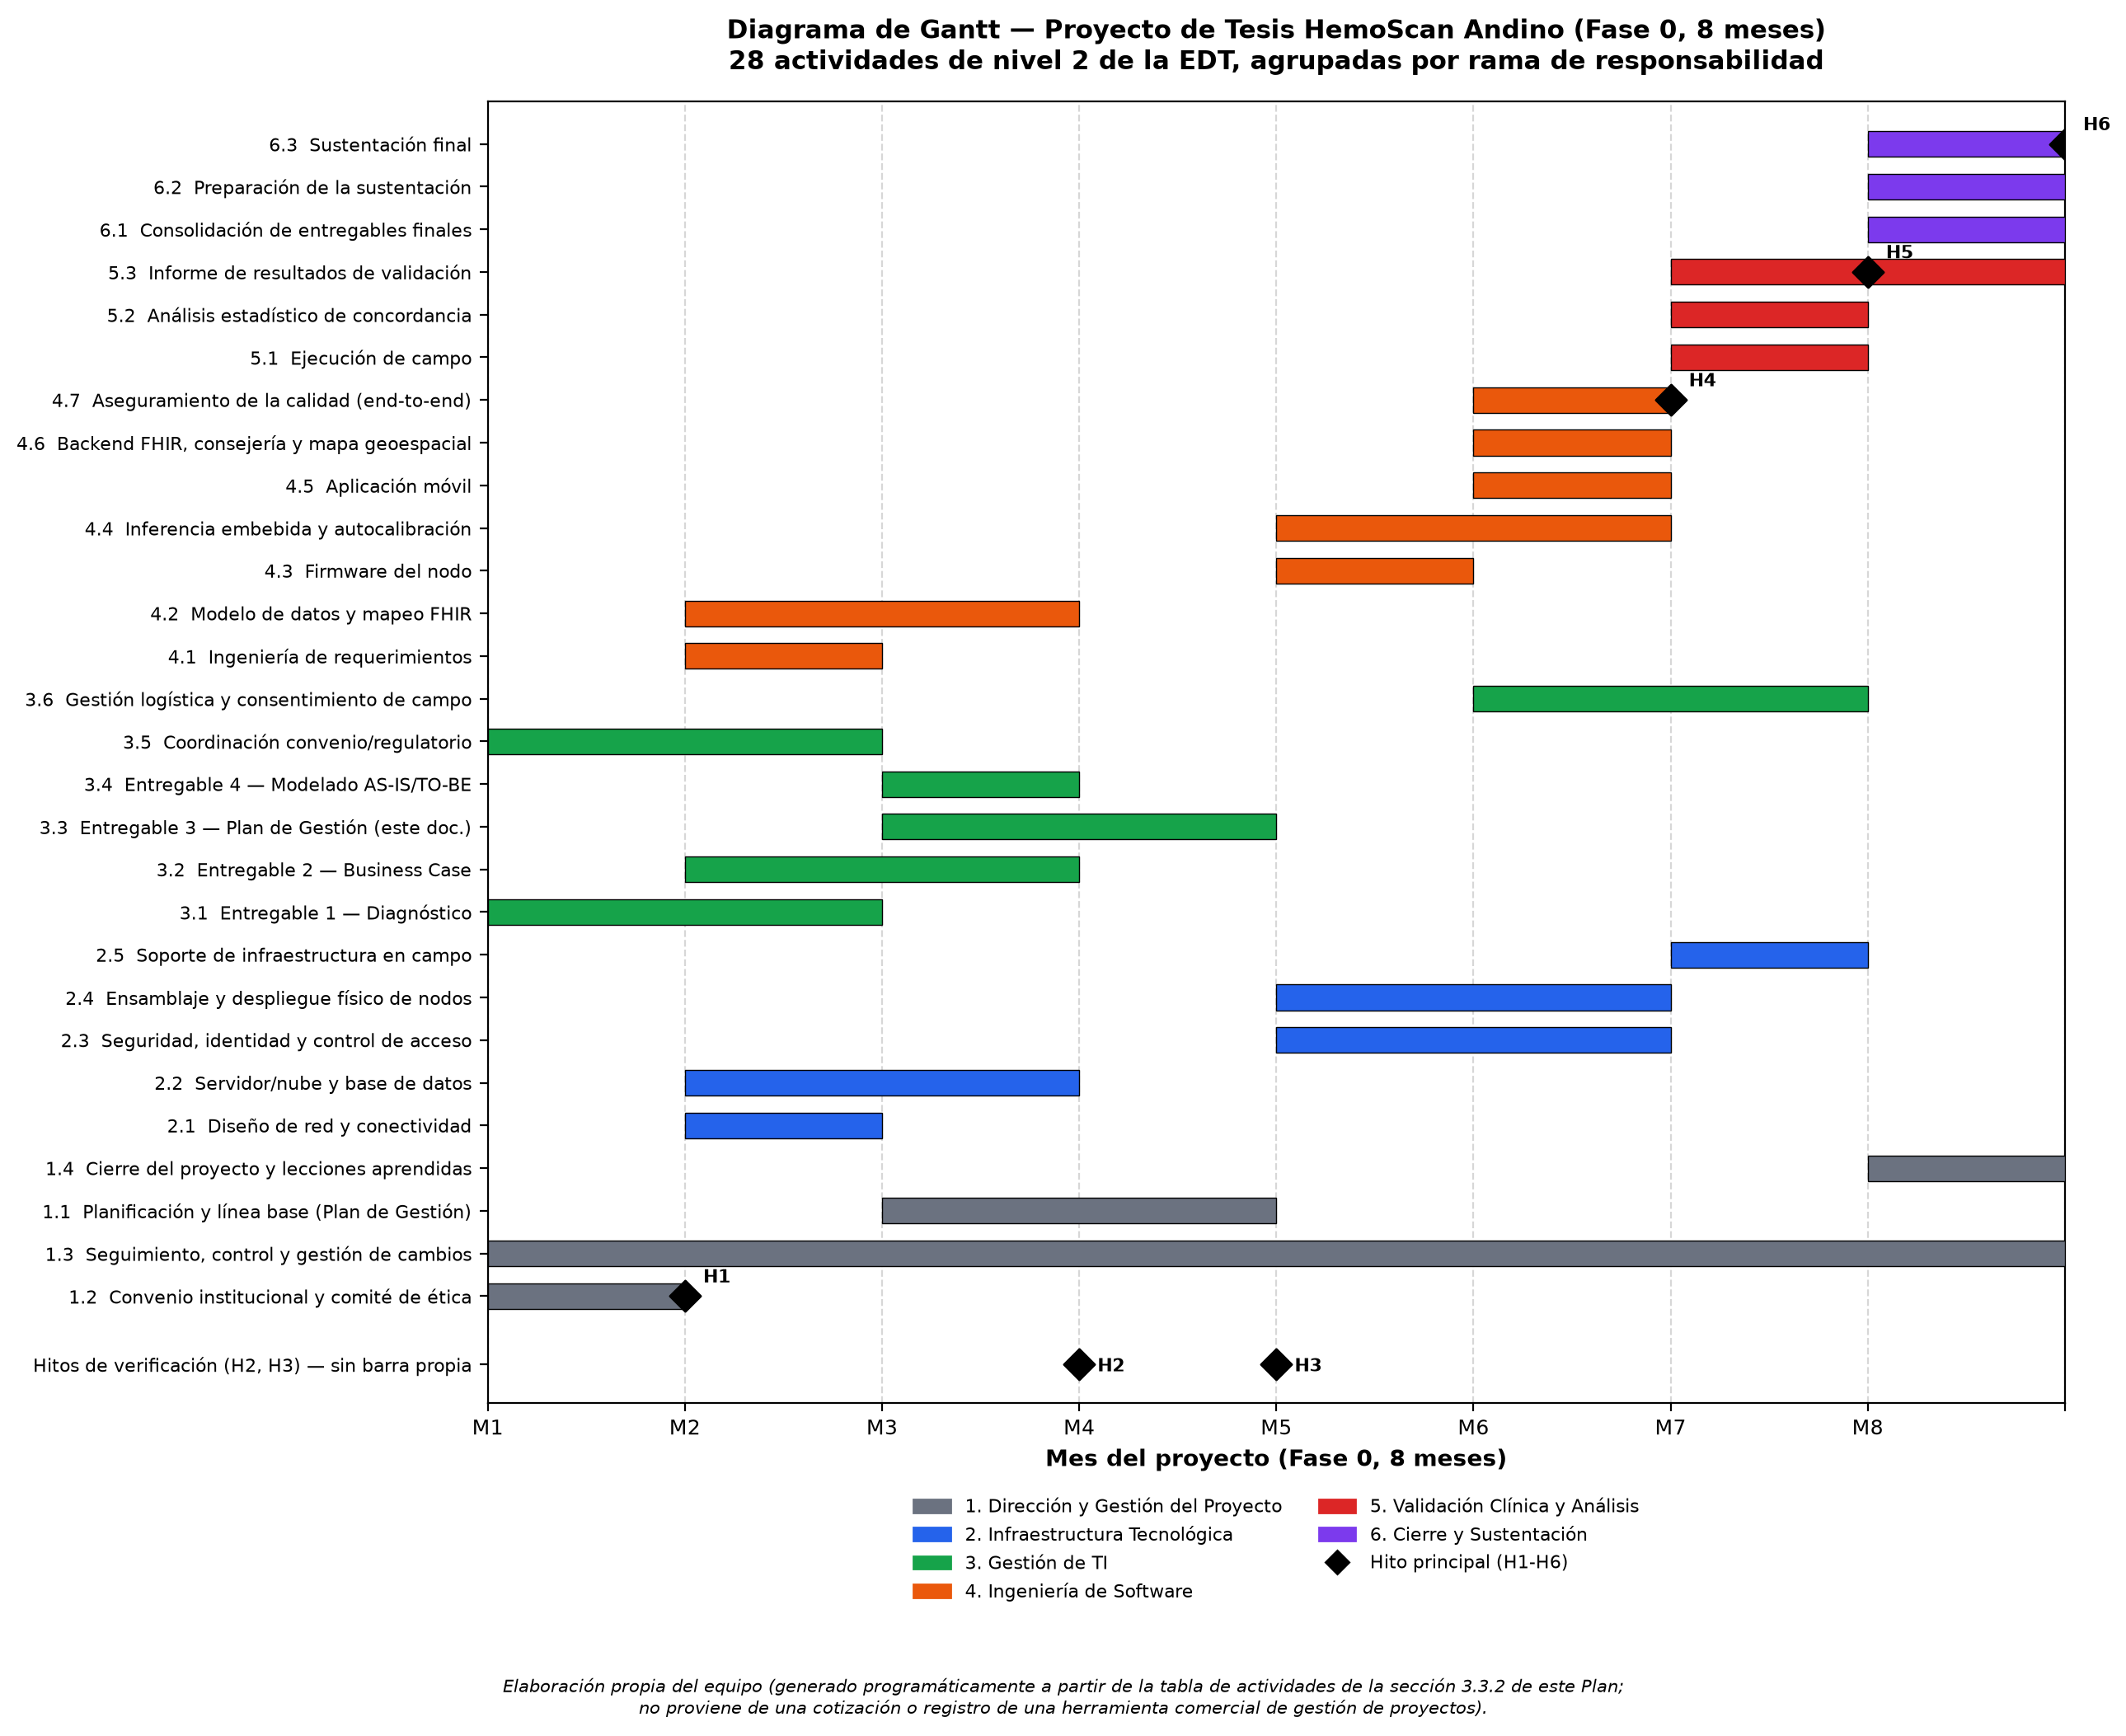
\includegraphics[width=0.88\linewidth,keepaspectratio]{assets/03-plan-gestion/gantt-diagrama.png}}
\caption{Diagrama de Gantt gráfico --- HemoScan Andino, Proyecto de Tesis (Fase 0, 8 meses)}
\end{figure}

\emph{Figura 2b. Diagrama de Gantt gráfico de las 28 actividades de nivel 2 de la EDT (sección 3.3.2), agrupadas por rama de responsabilidad, con los 6 hitos principales (H1-H6, sección 3.3.4) señalados con marcadores en forma de diamante. Elaboración propia del equipo: generado programáticamente a partir de la misma tabla de datos de la sección 3.3.2 (no proviene de una cotización o de un registro exportado de una herramienta comercial de gestión de proyectos como MS Project; se declara así por honestidad metodológica, en línea con el resto de este documento).}

\subsubsection{3.3.4 Hitos principales}\label{hitos-principales}

{\small
\begin{longtable}[]{@{}
  >{\raggedright\arraybackslash}p{(\linewidth - 6\tabcolsep) * \real{0.2500}}
  >{\raggedright\arraybackslash}p{(\linewidth - 6\tabcolsep) * \real{0.2500}}
  >{\raggedright\arraybackslash}p{(\linewidth - 6\tabcolsep) * \real{0.2500}}
  >{\raggedright\arraybackslash}p{(\linewidth - 6\tabcolsep) * \real{0.2500}}@{}}
\toprule\noalign{}
\begin{minipage}[b]{\linewidth}\raggedright
Código
\end{minipage} & \begin{minipage}[b]{\linewidth}\raggedright
Hito
\end{minipage} & \begin{minipage}[b]{\linewidth}\raggedright
Momento
\end{minipage} & \begin{minipage}[b]{\linewidth}\raggedright
Criterio de verificación
\end{minipage} \\
\midrule\noalign{}
\endhead
\bottomrule\noalign{}
\endlastfoot
H1 & Convenio institucional y comité de ética formalizados & Fin de Mes 1 & Convenio firmado + dictamen ético emitido (o activación documentada del plan de contingencia, sección 3.5.3) \\
H2 & Diseño técnico y protocolo de validación cerrados & Fin de Mes 3 & Documentos de arquitectura (2.1, 4.1, 4.2) y protocolo de validación clínica aprobados internamente \\
H3 & Cierre del semestre 1 (sustentación parcial) & Fin de Mes 4 & Los 4 entregables académicos aprobados por el docente asesor \\
H4 & Prototipo integrado listo & Fin de Mes 6 & \textgreater= 90 \% de casos de prueba end-to-end (paquete 4.7) superados \\
H5 & Validación de campo completada & Fin de Mes 7 & Base de datos de campo completa + informe preliminar de resultados (5.3) \\
H6 & Sustentación final aprobada & Fin de Mes 8 & Acta de sustentación con resultado aprobatorio \\
\end{longtable}
}

Estos seis hitos corresponden, de manera exactamente correlativa, a las seis fases macro del proyecto ya definidas (sección 3.3.1), de modo que el cumplimiento de cada hito es, a la vez, el criterio de salida de su fase y el criterio de entrada de la siguiente.

\subsubsection{3.3.5 Análisis de ruta crítica}\label{anuxe1lisis-de-ruta-cruxedtica}

El análisis de la red de precedencias de la sección 3.3.2 muestra que, bajo el supuesto de que el convenio institucional y la aprobación ética se formalizan dentro del plazo previsto (Mes 1, riesgo RP1 controlado), la \textbf{ruta crítica del proyecto discurre íntegramente por la cadena de construcción técnica}: 4.1 (requerimientos) -\textgreater{} 4.2 (modelo de datos/FHIR) -\textgreater{} 4.3 (firmware) -\textgreater{} 4.4 (inferencia y autocalibración) -\textgreater{} 4.5/4.6 (app y backend, en paralelo) -\textgreater{} 4.7 (aseguramiento de calidad) -\textgreater{} 5.1 (campo) -\textgreater{} 5.2 (análisis) -\textgreater{} 5.3 (informe) -\textgreater{} 6.1-6.3 (cierre y sustentación), con una duración acumulada que ocupa del Mes 2 al Mes 8 del proyecto. Esta cadena determina la fecha de sustentación final y no tiene holgura (float) disponible: cualquier retraso en el paquete 4.3, 4.4 o 4.7 se traslada directamente a la fecha de la validación de campo (Mes 7) y, por tanto, a la sustentación (Mes 8).

Un segundo hallazgo, de mayor relevancia para la gestión de riesgos (sección 3.5), es que el paquete \textbf{1.2 (convenio institucional y comité de ética, Mes 1) no forma parte de la ruta crítica bajo el escenario normal}, dado que el trabajo técnico (rama 4) puede avanzar en paralelo sin depender de la firma del convenio; sin embargo, \textbf{su holgura es engañosamente pequeña}, porque el paquete 5.1 (ejecución de campo, Mes 7) sí depende estrictamente de 1.2. En otras palabras, 1.2 tiene holgura frente a la ruta crítica técnica solo mientras su atraso no exceda, aproximadamente, los cinco meses que separan el Mes 1 del inicio del Mes 7 ---un margen que parece amplio, pero que en la práctica se consume rápidamente si el convenio se retrasa más allá del Mes 2, dado que la gestión institucional real (identificación de una microred, negociación, aprobación de un comité de ética) rara vez es instantánea una vez iniciado el atraso. Por esta razón, 1.2 se trata en este Plan como una \textbf{ruta casi crítica (near-critical path)} que requiere seguimiento prioritario desde la primera semana del proyecto, y se refuerza con un plan de contingencia específico (sección 3.5.3), en lugar de asumir con optimismo que su holgura nominal de varios meses elimina el riesgo.

Finalmente, la cadena de entregables académicos (3.1 -\textgreater{} 3.2/3.4 -\textgreater{} 3.3, Meses 1 a 4) tiene, en términos de red de precedencias pura, cierta holgura frente a la ruta crítica técnica (que se extiende hasta el Mes 8); no obstante, el hito H3 (cierre del semestre 1, Mes 4) es un \textbf{hito institucional de fecha fija impuesto por el calendario académico de la universidad}, no derivado del cálculo de la red. En consecuencia, el equipo trata este hito con holgura cero en la práctica, independientemente de lo que indique el análisis de red, en línea con la buena práctica de distinguir entre holgura calculada y restricciones de tipo ``fecha obligatoria'' (must-finish-on) en la gestión de cronogramas.

\begin{center}\rule{0.5\linewidth}{0.5pt}\end{center}

\subsection{3.4 Gestión de Costos}\label{gestiuxf3n-de-costos}

\subsubsection{3.4.1 Presupuesto detallado}\label{presupuesto-detallado}

El presupuesto total de este proyecto es de \textbf{S/ 3,124}, cifra ya comprometida y detallada en el Business Case (Entregable 2, sección 2.4.1), y que se reproduce aquí asignada a su paquete de la EDT, su mes de ejecución principal y su responsable, para que constituya una línea base de costos gestionable dentro de este Plan:

{\small
\begin{longtable}[]{@{}
  >{\raggedright\arraybackslash}p{(\linewidth - 8\tabcolsep) * \real{0.2000}}
  >{\raggedright\arraybackslash}p{(\linewidth - 8\tabcolsep) * \real{0.2000}}
  >{\raggedright\arraybackslash}p{(\linewidth - 8\tabcolsep) * \real{0.2000}}
  >{\raggedright\arraybackslash}p{(\linewidth - 8\tabcolsep) * \real{0.2000}}
  >{\raggedright\arraybackslash}p{(\linewidth - 8\tabcolsep) * \real{0.2000}}@{}}
\toprule\noalign{}
\begin{minipage}[b]{\linewidth}\raggedright
Partida
\end{minipage} & \begin{minipage}[b]{\linewidth}\raggedright
Monto (S/)
\end{minipage} & \begin{minipage}[b]{\linewidth}\raggedright
Paquete EDT relacionado
\end{minipage} & \begin{minipage}[b]{\linewidth}\raggedright
Mes(es) de ejecución
\end{minipage} & \begin{minipage}[b]{\linewidth}\raggedright
Responsable
\end{minipage} \\
\midrule\noalign{}
\endhead
\bottomrule\noalign{}
\endlastfoot
Hardware (3 nodos) & 900 & 2.4 --- Ensamblaje y despliegue físico de los nodos & M5-M6 & Integrante 1 \\
Insumos de validación HemoCue & 400 & 5.1 --- Ejecución de campo & M7 & Integrante 2 \\
Submuestra ferritina + PCR & 600 & 5.1 --- Ejecución de campo & M7 & Integrante 2 \\
Servidor/nube (8 meses) & 320 & 2.2 --- Servidor/nube y base de datos & M1-M8 (continuo, S/ 40/mes) & Integrante 1 \\
Impresión 3D & 120 & 2.4 --- Ensamblaje y despliegue físico de los nodos & M5-M6 & Integrante 1 \\
Movilidad/campo & 400 & 1.2 (M1, gestión de convenio) y 5.1 (M7, campo) & M1 (S/ 100) y M7 (S/ 300) & Integrante 2 \\
Materiales de gestión & 100 & 1.1/1.3 --- Planificación y seguimiento & M1, M4, M7, M8 (S/ 25 c/u) & Integrante 2 \\
Contingencia (10 \%) & 284 & Reserva transversal del proyecto & Distribuida a lo largo de los 8 meses (ver 3.4.2) & Integrante 2 (custodio de la reserva) \\
\textbf{TOTAL} & \textbf{3,124} & & & \\
\end{longtable}
}

Esta asignación por paquete EDT y mes es una \textbf{construcción interna del equipo} para fines de programación y control (no proviene de una cotización desagregada por fecha de proveedores) y es consistente, en su cifra total, con el egreso de S/ 3,124 ya reportado como ``Año 0 (Fase 0)'' en el Anexo C del Business Case (Entregable 2), lo que garantiza continuidad financiera entre ambos documentos.

\paragraph{3.4.1.1 Desglose referencial de costo unitario (evidencia externa de mercado)}\label{desglose-referencial-de-costo-unitario-evidencia-externa-de-mercado}

Una verificación adversarial de este Plan frente a la rúbrica observó que, si bien el monto total (S/ 3,124) es una cifra real y comprometida (heredada del Business Case), la única fuente de trazabilidad del presupuesto detallado de la sección 3.4.1 era la reasignación interna del equipo, sin desglose de costo unitario por componente ni fuente de mercado de referencia. Para sostener la exigencia de ``estimaciones justificadas'' del nivel Excelente de la rúbrica, se incorpora a continuación un desglose referencial de costo unitario, construido con rangos de mercado consultados por el equipo --- \textbf{no con cotizaciones formales de proveedores con fecha}, que a la fecha de este documento no existen (ver Anexo E, supuesto SP9). Cada fila señala explícitamente su condición de dato pendiente de validar.

\textbf{Tabla 3.4.1-A. Componentes de hardware (partida ``Hardware (3 nodos)'', S/ 900).}

{\small
\begin{longtable}[]{@{}
  >{\raggedright\arraybackslash}p{(\linewidth - 10\tabcolsep) * \real{0.1667}}
  >{\raggedright\arraybackslash}p{(\linewidth - 10\tabcolsep) * \real{0.1667}}
  >{\raggedright\arraybackslash}p{(\linewidth - 10\tabcolsep) * \real{0.1667}}
  >{\raggedright\arraybackslash}p{(\linewidth - 10\tabcolsep) * \real{0.1667}}
  >{\raggedright\arraybackslash}p{(\linewidth - 10\tabcolsep) * \real{0.1667}}
  >{\raggedright\arraybackslash}p{(\linewidth - 10\tabcolsep) * \real{0.1667}}@{}}
\toprule\noalign{}
\begin{minipage}[b]{\linewidth}\raggedright
Componente
\end{minipage} & \begin{minipage}[b]{\linewidth}\raggedright
Cantidad (3 nodos)
\end{minipage} & \begin{minipage}[b]{\linewidth}\raggedright
Rango de precio unitario referencial (S/)
\end{minipage} & \begin{minipage}[b]{\linewidth}\raggedright
Valor usado
\end{minipage} & \begin{minipage}[b]{\linewidth}\raggedright
Subtotal referencial (S/)
\end{minipage} & \begin{minipage}[b]{\linewidth}\raggedright
Fuente / naturaleza del dato
\end{minipage} \\
\midrule\noalign{}
\endhead
\bottomrule\noalign{}
\endlastfoot
Microcontrolador ESP32-S3 (DevKit-C1/WROOM o equivalente) & 3 & 30 -- 45 & 35 & \textasciitilde= 105 & Rango de mercado referencial de tiendas de electrónica e importadores (AliExpress, Mercado Libre Perú), consultado por el equipo --- \textbf{{[}DATO PENDIENTE DE VALIDAR: cotización formal con fecha y proveedor específico{]}} \\
Sensor espectral AS7341 (breakout, 10 canales + NIR/flicker) & 3 & 60 -- 85 & 70 & \textasciitilde= 210 & Ídem --- \textbf{{[}DATO PENDIENTE DE VALIDAR{]}} \\
Sensor óptico PPG/SpO2 MAX30102 (breakout) & 3 & 12 -- 22 & 18 & \textasciitilde= 54 & Ídem --- \textbf{{[}DATO PENDIENTE DE VALIDAR{]}} \\
LED blanco alto CRI (\textgreater= 90 CRI, montaje SMD) + óptica difusora simple & 3 (más repuestos) & 6 -- 12 & 8 & \textasciitilde= 24 & Ídem --- \textbf{{[}DATO PENDIENTE DE VALIDAR{]}} \\
\textbf{Subtotal componentes electrónicos activos (MCU + sensores + LED)} & & & & \textbf{\textasciitilde= 393} & Suma de las 4 filas anteriores \\
Conectores, cableado, batería recargable Li-Po, hardware de montaje/protoboard y stock de repuesto ante fallas de ensamblaje & 3 kits & --- (sin desglose unitario disponible) & --- & \textbf{\textasciitilde= 507 (por diferencia frente al monto ya comprometido de la partida)} & Estimación agregada del equipo, sin cotización unitaria --- \textbf{{[}DATO PENDIENTE DE VALIDAR: cotización desagregada del kit de montaje por componente{]}} \\
\textbf{TOTAL partida ``Hardware (3 nodos)'' (igual a la sección 3.4.1)} & & & & \textbf{900} & Cifra ya comprometida; el desglose de esta tabla es referencial y no altera el monto total \\
\end{longtable}
}

\emph{(La partida ``Impresión 3D'' de S/ 120, sección 3.4.1, ya está presupuestada por separado y no se duplica en esta tabla.)}

\textbf{Tabla 3.4.1-B. Insumos de validación clínica de campo (partidas ``Insumos de validación HemoCue'' S/ 400 y ``Submuestra ferritina + PCR'' S/ 600, Mes 7).}

{\small
\begin{longtable}[]{@{}
  >{\raggedright\arraybackslash}p{(\linewidth - 8\tabcolsep) * \real{0.2000}}
  >{\raggedright\arraybackslash}p{(\linewidth - 8\tabcolsep) * \real{0.2000}}
  >{\raggedright\arraybackslash}p{(\linewidth - 8\tabcolsep) * \real{0.2000}}
  >{\raggedright\arraybackslash}p{(\linewidth - 8\tabcolsep) * \real{0.2000}}
  >{\raggedright\arraybackslash}p{(\linewidth - 8\tabcolsep) * \real{0.2000}}@{}}
\toprule\noalign{}
\begin{minipage}[b]{\linewidth}\raggedright
Insumo
\end{minipage} & \begin{minipage}[b]{\linewidth}\raggedright
Base de cálculo asumida
\end{minipage} & \begin{minipage}[b]{\linewidth}\raggedright
Costo unitario referencial (S/)
\end{minipage} & \begin{minipage}[b]{\linewidth}\raggedright
Subtotal referencial (S/)
\end{minipage} & \begin{minipage}[b]{\linewidth}\raggedright
Fuente / naturaleza del dato
\end{minipage} \\
\midrule\noalign{}
\endhead
\bottomrule\noalign{}
\endlastfoot
Microcuvetas HemoCue Hb (o equivalente, método de referencia) & \textasciitilde= 300 determinaciones (límite superior de la submuestra de 150-300 niños, sección 3.1.1) + margen por repeticiones y control de calidad & \textasciitilde= 1.3 & \textasciitilde= 400 & Rango internacional referencial para microcuvetas HemoCue (del orden de USD 0.35-0.55 por unidad al tipo de cambio de referencia), consultado por el equipo --- \textbf{{[}DATO PENDIENTE DE VALIDAR: cotización del distribuidor autorizado de HemoCue en Perú, con fecha{]}} \\
Reactivos/kits de ferritina sérica y proteína C-reactiva (PCR), por determinación, sobre una submuestra interna de contraste (no toda la submuestra de 150-300 recibe ambos marcadores) & Número real de determinaciones \textbf{no definido aún} por el equipo & No estimado por unidad (variable según se procese en laboratorio propio o se tercerice) & 600 (techo de partida heredado del Business Case, Entregable 2) & Monto agregado sin desglose por número de determinaciones ni proveedor de laboratorio --- \textbf{{[}DATO PENDIENTE DE VALIDAR: número de determinaciones planificadas y cotización del laboratorio/proveedor de reactivos{]}} \\
\end{longtable}
}

Se declara explícitamente, con la misma honestidad metodológica del resto de este Plan, que los valores de las Tablas 3.4.1-A y 3.4.1-B son \textbf{estimaciones referenciales de mercado}, útiles para sustentar que el monto total de cada partida es plausible frente a precios reales observables, pero que \textbf{no sustituyen una cotización formal desagregada por fecha y proveedor}; dicha cotización sigue siendo, en su totalidad, un \textbf{{[}DATO PENDIENTE DE VALIDAR{]}} que el equipo deberá levantar antes de comprometer la orden de compra real en el Mes 3-4 (ver riesgo RP7, sección 3.5.2).

\subsubsection{3.4.2 Línea base de costos}\label{luxednea-base-de-costos}

A partir de la distribución mensual de cada partida (sección 3.4.1), se construye la siguiente línea base de costos acumulada, verificada aritméticamente: la suma de los costos directos mensuales reproduce exactamente el subtotal de S/ 2,840 ya reportado en el Business Case (antes de la contingencia), y la reserva de contingencia se prorratea de forma lineal a lo largo de los 8 meses (S/ 284 ÷ 8 = S/ 35.5/mes) para efectos de una línea base suave y gestionable, sin que ello implique que la contingencia se ``gasta'' mensualmente: es una reserva disponible en su totalidad desde el inicio, prorrateada aquí únicamente para fines de graficación de la curva S.

{\small
\begin{longtable}[]{@{}
  >{\raggedright\arraybackslash}p{(\linewidth - 10\tabcolsep) * \real{0.1667}}
  >{\raggedright\arraybackslash}p{(\linewidth - 10\tabcolsep) * \real{0.1667}}
  >{\raggedright\arraybackslash}p{(\linewidth - 10\tabcolsep) * \real{0.1667}}
  >{\raggedright\arraybackslash}p{(\linewidth - 10\tabcolsep) * \real{0.1667}}
  >{\raggedright\arraybackslash}p{(\linewidth - 10\tabcolsep) * \real{0.1667}}
  >{\raggedright\arraybackslash}p{(\linewidth - 10\tabcolsep) * \real{0.1667}}@{}}
\toprule\noalign{}
\begin{minipage}[b]{\linewidth}\raggedright
Mes
\end{minipage} & \begin{minipage}[b]{\linewidth}\raggedright
Costo directo del mes (S/)
\end{minipage} & \begin{minipage}[b]{\linewidth}\raggedright
Costo directo acumulado (S/)
\end{minipage} & \begin{minipage}[b]{\linewidth}\raggedright
Reserva de contingencia acumulada (S/)
\end{minipage} & \begin{minipage}[b]{\linewidth}\raggedright
\textbf{Presupuesto acumulado total --- línea base (S/)}
\end{minipage} & \begin{minipage}[b]{\linewidth}\raggedright
\% acumulado de la línea base
\end{minipage} \\
\midrule\noalign{}
\endhead
\bottomrule\noalign{}
\endlastfoot
M1 & 165.0 & 165.0 & 35.5 & 200.5 & 6.4 \% \\
M2 & 40.0 & 205.0 & 71.0 & 276.0 & 8.8 \% \\
M3 & 40.0 & 245.0 & 106.5 & 351.5 & 11.3 \% \\
M4 & 65.0 & 310.0 & 142.0 & 452.0 & 14.5 \% \\
M5 & 550.0 & 860.0 & 177.5 & 1,037.5 & 33.2 \% \\
M6 & 550.0 & 1,410.0 & 213.0 & 1,623.0 & 52.0 \% \\
M7 & 1,365.0 & 2,775.0 & 248.5 & 3,023.5 & 96.8 \% \\
M8 & 65.0 & 2,840.0 & 284.0 & \textbf{3,124.0} & \textbf{100.0 \%} \\
\end{longtable}
}

\textbf{Representación visual de la curva S de costos acumulados (escala: 1 bloque \textasciitilde= 5 \% del presupuesto total):}

\begin{samepage}\begin{verbatim}
M1  #...................   6.4 %   (S/    200.5)
M2  ##..................   8.8 %   (S/    276.0)
M3  ##..................  11.3 %   (S/    351.5)
M4  ###.................  14.5 %   (S/    452.0)
M5  #######.............  33.2 %   (S/  1,037.5)
M6  ##########..........  52.0 %   (S/  1,623.0)
M7  ###################.  96.8 %   (S/  3,023.5)
M8  #################### 100.0 %   (S/  3,124.0)
\end{verbatim}\end{samepage}

La lectura de esta curva S es coherente con el resto del Plan: el gasto es bajo y estable durante la gestión del convenio y el diseño (Meses 1 a 4, alcanzando apenas 14.5 \% del presupuesto), se acelera fuertemente durante la implementación (Meses 5-6, por la compra y ensamblaje del hardware) y alcanza su mayor concentración en el Mes 7 (validación de campo), que por sí solo representa cerca del 44 \% del presupuesto total (insumos HemoCue, submuestra de ferritina/PCR y movilidad de campo), consistente con el hecho de que la validación clínica es, tanto operativa como financieramente, la actividad de mayor intensidad de recursos de todo el proyecto.

\subsubsection{3.4.3 Fuente de financiamiento}\label{fuente-de-financiamiento}

El presupuesto de S/ 3,124 es financiado en su totalidad mediante \textbf{aporte propio del equipo de tesis} (autofinanciamiento), tal como ya se estableció en el Business Case (Entregable 2) como la única cifra financiera comprometida ---no ilustrativa--- de todo el proyecto. No se ha gestionado ni confirmado a la fecha ninguna fuente de financiamiento adicional (fondo concursable universitario, premio de innovación, cooperación internacional): \textbf{{[}DATO PENDIENTE DE VALIDAR: gestión de fuentes de financiamiento complementarias, si el equipo decidiera buscarlas antes o durante la ejecución{]}}. Esta condición refuerza la importancia del control presupuestal estricto descrito a continuación, dado que no existe una reserva de gestión (management reserve) adicional a la contingencia del 10 \% ya presupuestada.

\subsubsection{3.4.4 Mecanismo de control presupuestal}\label{mecanismo-de-control-presupuestal}

Dado que el proyecto no ha iniciado su ejecución, este Plan define ---sin poder todavía aplicar--- el mecanismo de control presupuestal que regirá la Fase 0, basado en una adaptación ligera de la Gestión del Valor Ganado (Earned Value Management, PMI):

\begin{enumerate}
\def\labelenumi{\arabic{enumi}.}
\tightlist
\item
  \textbf{Valor Planificado (PV).} Corresponde a la línea base de costos acumulada de la tabla de la sección 3.4.2, verificada mes a mes.
\item
  \textbf{Valor Ganado (EV) y Costo Real (AC).} En cada hito principal (H1 a H6, sección 3.3.4), el Director/a de Proyecto calculará el EV como el costo presupuestado de los paquetes de la EDT efectivamente completados, y el AC como el gasto real ejecutado a esa fecha, con soporte de comprobantes.
\item
  \textbf{Índices de desempeño.} Se calcularán el Índice de Desempeño del Costo (CPI = EV/AC) y el Índice de Desempeño del Cronograma (SPI = EV/PV) en cada hito.
\item
  \textbf{Umbrales de control.} Un CPI o SPI entre 0.90 y 1.10 se considera dentro de tolerancia normal. Un valor entre 0.75 y 0.90 activa una revisión de variación en la siguiente reunión de seguimiento (paquete 1.3) y puede autorizar el uso parcial de la reserva de contingencia (S/ 284). Un valor por debajo de 0.75 se considera una variación severa que obliga a una solicitud formal de cambio (sección 3.2.4) y a informar al docente asesor, evaluando opciones de mitigación (redistribución de horas, reducción acotada del alcance no crítico, o búsqueda de financiamiento adicional).
\item
  \textbf{Custodia de la reserva.} La liberación de cualquier monto de la reserva de contingencia requiere justificación escrita del Director/a de Proyecto (Integrante 2) y registro en la bitácora de control de cambios (sección 3.2.4), evitando su uso informal o no documentado.
\end{enumerate}

\subsubsection{3.4.5 Relación con el presupuesto de las Fases 1 y 2}\label{relaciuxf3n-con-el-presupuesto-de-las-fases-1-y-2}

Se reitera, para evitar duplicación entre entregables, que el presupuesto y los indicadores financieros de la Fase 1 (piloto pagado) y de la Fase 2 (escalamiento) ---incluyendo el modelo financiero a tres años, el VAN (\textasciitilde= S/ 952), la TIR (\textasciitilde= 23.4 \%) y el punto de equilibrio (\textasciitilde= 6 establecimientos, tras la corrección aritmética documentada en el Anexo C del Business Case)--- ya fueron desarrollados en el Business Case (Entregable 2, secciones 2.3 y 2.4) y \textbf{no forman parte de la línea base de costos de este Plan de Gestión}, cuyo alcance se circunscribe estrictamente al presupuesto de S/ 3,124 de la Fase 0 (sección 3.1.4). Cualquier decisión de transición presupuestal hacia la Fase 1 queda fuera del alcance de este documento y correspondería a una actualización del Business Case una vez formalizado un contrato o convenio de piloto pagado.

\begin{center}\rule{0.5\linewidth}{0.5pt}\end{center}

\subsection{3.5 Gestión de Riesgos}\label{gestiuxf3n-de-riesgos}

\subsubsection{3.5.1 Alcance de este registro de riesgos frente al Business Case}\label{alcance-de-este-registro-de-riesgos-frente-al-business-case}

El Business Case (Entregable 2, sección 2.5) ya desarrolló un registro de doce \textbf{riesgos estratégicos de negocio} (R1-R12), de naturaleza comercial, regulatoria y financiera, con un alcance explícitamente preliminar. Este Plan de Gestión desarrolla un registro complementario, no redundante, de \textbf{riesgos de ejecución del proyecto de ocho meses} (identificados como RP1-RP12, ``Riesgo de Proyecto''), centrado en amenazas al cronograma, el alcance, el costo, la calidad técnica y los recursos de este Plan. Varios riesgos de ejecución están vinculados a un riesgo estratégico equivalente del Business Case, lo cual se indica explícitamente en cada ficha, reforzando la coherencia entre ambos documentos.

\subsubsection{3.5.2 Identificación y análisis cualitativo de riesgos}\label{identificaciuxf3n-y-anuxe1lisis-cualitativo-de-riesgos}

{\small
\begin{longtable}[]{@{}
  >{\raggedright\arraybackslash}p{(\linewidth - 12\tabcolsep) * \real{0.1429}}
  >{\raggedright\arraybackslash}p{(\linewidth - 12\tabcolsep) * \real{0.1429}}
  >{\raggedright\arraybackslash}p{(\linewidth - 12\tabcolsep) * \real{0.1429}}
  >{\raggedright\arraybackslash}p{(\linewidth - 12\tabcolsep) * \real{0.1429}}
  >{\raggedright\arraybackslash}p{(\linewidth - 12\tabcolsep) * \real{0.1429}}
  >{\raggedright\arraybackslash}p{(\linewidth - 12\tabcolsep) * \real{0.1429}}
  >{\raggedright\arraybackslash}p{(\linewidth - 12\tabcolsep) * \real{0.1429}}@{}}
\toprule\noalign{}
\begin{minipage}[b]{\linewidth}\raggedright
N.°
\end{minipage} & \begin{minipage}[b]{\linewidth}\raggedright
Riesgo
\end{minipage} & \begin{minipage}[b]{\linewidth}\raggedright
Categoría
\end{minipage} & \begin{minipage}[b]{\linewidth}\raggedright
Probabilidad
\end{minipage} & \begin{minipage}[b]{\linewidth}\raggedright
Impacto
\end{minipage} & \begin{minipage}[b]{\linewidth}\raggedright
Nivel de riesgo
\end{minipage} & \begin{minipage}[b]{\linewidth}\raggedright
Vínculo con Business Case
\end{minipage} \\
\midrule\noalign{}
\endhead
\bottomrule\noalign{}
\endlastfoot
RP1 & Retraso en la firma del convenio institucional y/o la aprobación del comité de ética más allá del Mes 1, que posterga toda actividad dependiente (en particular, la ejecución de campo del Mes 7) & Cronograma / Institucional & Alta & Crítico & \textbf{Crítico} & R3 \\
RP2 & Disponibilidad horaria semanal insuficiente de uno o más integrantes por superposición con otros cursos o trabajo, que retrase paquetes de la ruta crítica & Recursos & Media & Alto & Alto & --- \\
RP3 & Fallas de integración entre los 3 sensores (AS7341, MAX30102, cámara) y el firmware ESP32-S3/BLE que excedan el tiempo asignado (Mes 5-6) & Técnico & Media & Alto & Alto & --- \\
RP4 & El modelo de inferencia embebido no alcanza los umbrales mínimos de sensibilidad (\textgreater= 85 \%) y especificidad (\textgreater= 80 \%) definidos en el protocolo de validación & Técnico / Clínico & Media & Crítico & \textbf{Crítico} & R2 \\
RP5 & Indisponibilidad o incumplimiento logístico durante la ejecución de campo (Mes 7): clima altiplánico, transporte, disponibilidad de familias & Operativo / Ambiental & Media & Alto & Alto & R12 \\
RP6 & Cambios de alcance no controlados (``scope creep'') por solicitudes adicionales del asesor o de la futura microred durante el desarrollo & Alcance & Media & Medio & Medio & --- \\
RP7 & Retraso en la entrega de componentes electrónicos importados (AS7341, MAX30102, ESP32-S3) que impacte el inicio de la implementación (Mes 5) & Cadena de suministro & Baja & Alto & Medio & R6 \\
RP8 & Brecha de protección de datos personales de menores durante la recolección de datos de campo (Mes 7) por controles insuficientes al momento de la validación & Legal / Datos personales & Baja & Crítico & Alto & R5 \\
RP9 & Ausencia, enfermedad o indisponibilidad temporal de un integrante durante una fase crítica del proyecto & Recursos humanos & Baja & Alto & Medio & R9 \\
RP10 & Descoordinación entre las 3 áreas del equipo (Infraestructura, Gestión, Software) que genere reprocesos por dependencias no gestionadas & Gestión / Integración & Media & Medio & Medio & --- \\
RP11 & Cambios en el calendario académico oficial de la universidad que compriman el tiempo disponible del Mes 4 o del Mes 8 & Institucional / Académico & Media & Medio & Medio & --- \\
RP12 & Los resultados de la validación de campo (Mes 7) resultan insuficientes, por tamaño de submuestra u otros factores estadísticos, para sustentar conclusiones sólidas en el Mes 8 & Metodológico & Baja & Alto & Medio & --- \\
\end{longtable}
}

\textbf{Mapa de calor cualitativo (probabilidad × impacto):}

\begin{samepage}\begin{verbatim}
                     Probabilidad: Baja          Probabilidad: Media          Probabilidad: Alta
Impacto Crítico  |   RP8                      |  RP4                       |  RP1
Impacto Alto     |   RP7, RP9, RP12           |  RP2, RP3, RP5             |  —
Impacto Medio    |   —                        |  RP6, RP10, RP11           |  —
Impacto Bajo     |   —                        |  —                        |  —
\end{verbatim}\end{samepage}

De los doce riesgos identificados, \textbf{dos se clasifican en nivel crítico}: RP1 (retraso del convenio/comité de ética) y RP4 (insuficiencia del modelo de inferencia frente a los umbrales clínicos), que además son, precisamente, la traducción a nivel de ejecución de los dos riesgos estratégicos ya calificados como críticos en el Business Case (R3 y R2, respectivamente). Esta correspondencia no es casual: refuerza que los dos factores más determinantes para el éxito del proyecto ---adopción/acceso institucional y validez clínica del algoritmo--- son consistentes a lo largo de los tres documentos de gestión ya elaborados (Diagnóstico, Business Case y este Plan).

\subsubsection{3.5.3 Plan de respuesta a riesgos}\label{plan-de-respuesta-a-riesgos}

Para cada riesgo se define una estrategia de respuesta (evitar, mitigar, transferir o aceptar) y una acción específica con responsable asignado:

{\small
\begin{longtable}[]{@{}
  >{\raggedright\arraybackslash}p{(\linewidth - 6\tabcolsep) * \real{0.2500}}
  >{\raggedright\arraybackslash}p{(\linewidth - 6\tabcolsep) * \real{0.2500}}
  >{\raggedright\arraybackslash}p{(\linewidth - 6\tabcolsep) * \real{0.2500}}
  >{\raggedright\arraybackslash}p{(\linewidth - 6\tabcolsep) * \real{0.2500}}@{}}
\toprule\noalign{}
\begin{minipage}[b]{\linewidth}\raggedright
N.°
\end{minipage} & \begin{minipage}[b]{\linewidth}\raggedright
Estrategia
\end{minipage} & \begin{minipage}[b]{\linewidth}\raggedright
Acción específica
\end{minipage} & \begin{minipage}[b]{\linewidth}\raggedright
Responsable
\end{minipage} \\
\midrule\noalign{}
\endhead
\bottomrule\noalign{}
\endlastfoot
RP1 & Mitigar + Plan de contingencia formal (ver detalle abajo) & Iniciar gestiones institucionales desde el día 1 del proyecto; identificar 2-3 microrredes candidatas en paralelo (no solo una); preparar con antelación el expediente para el comité de ética & Integrante 2 \\
RP2 & Mitigar & Acordar y documentar la disponibilidad horaria semanal mínima de cada integrante antes del inicio del Mes 2 (cierra el supuesto SP2); monitoreo semanal en las reuniones de seguimiento & Integrante 2 (seguimiento) / todo el equipo \\
RP3 & Mitigar & Incluir pruebas de concepto (spikes) de la integración crítica durante los sprints de diseño (Sprints 1 y 3, sección 3.6) antes de comprometer fechas de producción; reservar 1 semana de colchón técnico dentro del Mes 6 & Integrante 3 (con apoyo de Integrante 1) \\
RP4 & Mitigar + Aceptar residualmente & Reservar un ciclo de reajuste algorítmico dentro del Mes 6, antes de comprometer el inicio del campo; si el umbral no se alcanza, reportarlo honestamente en el informe de validación en lugar de forzar una conclusión favorable & Integrante 3 (técnico) / Integrante 2 (reporte honesto) \\
RP5 & Mitigar & Planificar la jornada de campo con una ventana de reprogramación de al menos 1 semana dentro del propio Mes 7; coordinar fechas alternativas por comunidad con la Jefatura de microred & Integrante 2 (logística) / todo el equipo \\
RP6 & Mitigar & Aplicar estrictamente el procedimiento de control de cambios (sección 3.2.4); recordar el alcance preliminar aprobado en cada reunión de seguimiento & Integrante 2 \\
RP7 & Mitigar & Colocar el pedido de componentes tan pronto se cierre el diseño de hardware (fin de Mes 3), con 4-6 semanas de margen antes del Mes 5; identificar un proveedor alternativo de respaldo & Integrante 1 \\
RP8 & Evitar (controles preventivos) + Mitigar & No autorizar el inicio de la ejecución de campo (5.1) sin que el checklist de seguridad (2.3) y el flujo de consentimiento informado digital (HC08) estén verificados y firmados conjuntamente & Integrante 1 (controles técnicos) / Integrante 2 (consentimiento) \\
RP9 & Mitigar & Mantener una bitácora compartida y básica de avance técnico que permita continuidad ante una ausencia breve de cualquier integrante; evitar concentración de conocimiento crítico sin respaldo documental & Todo el equipo \\
RP10 & Mitigar & Reforzar la revisión de dependencias entre paquetes EDT en cada sprint planning (sección 3.6.3); dar seguimiento reforzado a la carga concentrada del Sprint 8 & Integrante 2 (coordinación) / todo el equipo \\
RP11 & Aceptar + Monitorear & Confirmar el calendario académico oficial con la Escuela Profesional en cuanto esté disponible; ajustar este Plan mediante el procedimiento de control de cambios si corresponde & Integrante 2 \\
RP12 & Mitigar + Aceptar residualmente & Solicitar al asesor metodológico la validación formal del tamaño muestral antes de finalizar el Mes 3 (hito H2); si resulta insuficiente, reportar honestamente el nivel de incertidumbre estadística en el informe de validación & Integrante 2 \\
\end{longtable}
}

\textbf{Plan de contingencia detallado para RP1 (retraso del convenio institucional/comité de ética).} Por ser el único riesgo de nivel crítico con probabilidad alta, se define un plan de contingencia escalonado:

\begin{enumerate}
\def\labelenumi{\arabic{enumi}.}
\tightlist
\item
  \textbf{Alerta temprana (semana 2 del Mes 1):} si no existe al menos una carta de intención o manifestación de interés de una microred candidata, se escala la gestión institucional con apoyo directo del docente asesor y, de ser posible, de la coordinación de la Escuela Profesional.
\item
  \textbf{Activación de candidatas alternativas (semana 3 del Mes 1):} si la microred candidata principal no responde, se activa formalmente el contacto con una segunda microred candidata identificada desde el inicio (evitando depender de una única vía de acceso institucional).
\item
  \textbf{Escalamiento formal (fin del Mes 1):} si al finalizar el Mes 1 no se ha formalizado ni el convenio ni la aprobación ética, se declara una variación de cronograma (procedimiento de la sección 3.2.4) y se evalúan dos opciones no excluyentes: (a) comprimir el Mes 2 destinando tiempo adicional a la gestión institucional en paralelo al inicio del diseño técnico (que no depende del convenio, según el análisis de ruta crítica de la sección 3.3.5), o (b) de persistir la imposibilidad de acceso a datos reales de menores hacia el Mes 3, sustituir la validación de campo planificada por una \textbf{validación de banco (bench validation) con datos de referencia documentados en la literatura y/o voluntarios adultos}, dejando expresamente consignado en la sustentación final que este escenario constituye una limitación metodológica significativa y no un sustituto equivalente de la validación clínica pediátrica originalmente planificada.
\item
  \textbf{Registro y trazabilidad:} cualquier activación de este plan de contingencia se documenta en el registro de control de cambios (sección 3.2.4) y se comunica formalmente al docente asesor.
\end{enumerate}

\begin{center}\rule{0.5\linewidth}{0.5pt}\end{center}

\subsection{3.6 Gestión Ágil}\label{gestiuxf3n-uxe1gil}

\subsubsection{3.6.1 Justificación del enfoque híbrido}\label{justificaciuxf3n-del-enfoque-huxedbrido}

Este Plan adopta un enfoque \textbf{híbrido PMBOK/Ágil}, y no uno puramente predictivo ni puramente ágil, por una razón estructural ya anticipada en la sección 3.3.1: los Meses 1, 4, 7 y 8 están gobernados por hitos de naturaleza \textbf{fija, institucional y no iterativa} (un convenio se firma o no se firma; una sustentación ocurre en una fecha determinada; una jornada de campo ejecuta un protocolo ya cerrado), para los cuales un marco predictivo de tipo stage-gate es más adecuado que Scrum, dado que no existe, en sentido estricto, un ``incremento de producto'' que entregar de forma iterativa durante la gestión de un convenio o durante una sustentación. En contraste, los Meses 2-3 (diseño) y 5-6 (implementación) concentran la \textbf{incertidumbre técnica real} del proyecto ---¿es viable la fusión sincronizada de las 3 señales ópticas?, ¿corre la inferencia embebida en el tiempo requerido?, ¿es auditable en la práctica la autocalibración por altitud?--- y por tanto se benefician de ciclos cortos, iterativos y verificables mediante incrementos de software/firmware funcionando, que es precisamente la propuesta de valor de un marco ágil tipo Scrum (Schwaber y Sutherland, 2020). Esta combinación no es una preferencia estética: es una decisión de diseño metodológico justificada por la naturaleza distinta de cada tramo del proyecto.

\subsubsection{3.6.2 Roles ágiles del equipo}\label{roles-uxe1giles-del-equipo}

Dado que el equipo de desarrollo tiene solo 3 integrantes ---y los 3 deben además ejecutar tareas fuera del desarrollo de software (gestión, infraestructura)---, los roles de Scrum se adaptan de la siguiente manera, en lugar de forzar una estructura pensada originalmente para equipos más grandes:

{\small
\begin{longtable}[]{@{}
  >{\raggedright\arraybackslash}p{(\linewidth - 4\tabcolsep) * \real{0.3333}}
  >{\raggedright\arraybackslash}p{(\linewidth - 4\tabcolsep) * \real{0.3333}}
  >{\raggedright\arraybackslash}p{(\linewidth - 4\tabcolsep) * \real{0.3333}}@{}}
\toprule\noalign{}
\begin{minipage}[b]{\linewidth}\raggedright
Rol ágil
\end{minipage} & \begin{minipage}[b]{\linewidth}\raggedright
Asignación
\end{minipage} & \begin{minipage}[b]{\linewidth}\raggedright
Adaptación específica de este equipo
\end{minipage} \\
\midrule\noalign{}
\endhead
\bottomrule\noalign{}
\endlastfoot
Product Owner & Integrante 2 (Líder de Gestión de TI) & Mantiene y prioriza el product backlog; representa, ante la ausencia de un cliente real confirmado, la voz de la Microred de Salud Altiplano-Puno (caso ilustrativo) y del docente asesor; define los criterios de aceptación con apoyo técnico de los otros dos integrantes \\
Scrum Master & Rotativo entre Integrante 1 e Integrante 3, cada 2 sprints & Facilita las ceremonias y remueve impedimentos; la rotación evita que el mismo integrante concentre simultáneamente el rol de Product Owner y de Scrum Master, preservando una separación mínima de responsabilidades pese al tamaño reducido del equipo \\
Equipo de desarrollo & Los 3 integrantes, de forma multifuncional & Cada integrante aporta su especialidad (hardware/infraestructura, gestión/validación, software) a las historias de usuario que correspondan, sin rigidez estricta de ``solo su área'' cuando el sprint lo requiera \\
\end{longtable}
}

\textbf{Ceremonias adoptadas (con adaptación explícita al contexto estudiantil de dedicación parcial):} Sprint Planning al inicio de cada sprint (1-2 horas); reuniones breves de coordinación 3 veces por semana en lugar de un daily estricto de Scrum, dado que los 3 integrantes no dedican tiempo completo al proyecto; Sprint Review al cierre de cada sprint, con demostración al docente asesor cuando su disponibilidad lo permita; y Sprint Retrospective al cierre de cada sprint. Esta adaptación de la cadencia de ceremonias se declara explícitamente como una desviación consciente de la guía estricta de Scrum (Schwaber y Sutherland, 2020), justificada por la naturaleza de dedicación parcial del equipo.

\subsubsection{3.6.3 Product backlog}\label{product-backlog}

El backlog se organiza en ocho épicas, siete de ellas trazables directamente a un componente técnico ya definido del proyecto o a una automatización del Entregable 4, y una octava dedicada al protocolo y la logística de la validación clínica:

{\small
\begin{longtable}[]{@{}
  >{\raggedright\arraybackslash}p{(\linewidth - 4\tabcolsep) * \real{0.3333}}
  >{\raggedright\arraybackslash}p{(\linewidth - 4\tabcolsep) * \real{0.3333}}
  >{\raggedright\arraybackslash}p{(\linewidth - 4\tabcolsep) * \real{0.3333}}@{}}
\toprule\noalign{}
\begin{minipage}[b]{\linewidth}\raggedright
Épica
\end{minipage} & \begin{minipage}[b]{\linewidth}\raggedright
Descripción
\end{minipage} & \begin{minipage}[b]{\linewidth}\raggedright
Paquete(s) EDT relacionado(s)
\end{minipage} \\
\midrule\noalign{}
\endhead
\bottomrule\noalign{}
\endlastfoot
E1 & Firmware y captura multisensor (ESP32-S3, AS7341, MAX30102, BLE, buffer offline) & 2.1, 2.4, 4.3 \\
E2 & Autocalibración por altitud y motor de inferencia embebida & 4.4 \\
E3 & Aplicación móvil Flutter/PWA offline-first & 4.5 \\
E4 & Backend interoperable FHIR & 4.6, 2.2 \\
E5 & Seguridad, identidad y control de acceso & 2.3 \\
E6 & Consejería nutricional basada en reglas (NTS 213-MINSA/DGIESP-2024) & 4.6 \\
E7 & Mapa de cobertura/riesgo geoespacial & 2.2, 4.6 \\
E8 & Protocolo y logística de la validación clínica & 3.6, 5.1 \\
\end{longtable}
}

\textbf{Nota editorial sobre esta subsección.} Para mantener la extensión del cuerpo principal de este Plan cercana al rango sugerido por la rúbrica (ver nota editorial de la Introducción y Autoevaluación final), las 25 historias de usuario se presentan aquí en \textbf{versión condensada} (identificador, título breve, épica, prioridad MoSCoW, story points y sprint). El texto narrativo completo en formato ``Como/quiero/para'' y los criterios de aceptación detallados de cada historia, sin ninguna omisión de contenido, se encuentran íntegros en el \textbf{Anexo F}.

\textbf{Backlog de Diseño (Sprints 1-4, Meses 2-3).} Estas historias producen artefactos de diseño y pruebas de concepto (spikes), no necesariamente software listo para campo:

{\small
\begin{longtable}[]{@{}
  >{\raggedright\arraybackslash}p{(\linewidth - 10\tabcolsep) * \real{0.1667}}
  >{\raggedright\arraybackslash}p{(\linewidth - 10\tabcolsep) * \real{0.1667}}
  >{\raggedright\arraybackslash}p{(\linewidth - 10\tabcolsep) * \real{0.1667}}
  >{\raggedright\arraybackslash}p{(\linewidth - 10\tabcolsep) * \real{0.1667}}
  >{\raggedright\arraybackslash}p{(\linewidth - 10\tabcolsep) * \real{0.1667}}
  >{\raggedright\arraybackslash}p{(\linewidth - 10\tabcolsep) * \real{0.1667}}@{}}
\toprule\noalign{}
\begin{minipage}[b]{\linewidth}\raggedright
ID
\end{minipage} & \begin{minipage}[b]{\linewidth}\raggedright
Título breve
\end{minipage} & \begin{minipage}[b]{\linewidth}\raggedright
Épica
\end{minipage} & \begin{minipage}[b]{\linewidth}\raggedright
MoSCoW
\end{minipage} & \begin{minipage}[b]{\linewidth}\raggedright
Story points
\end{minipage} & \begin{minipage}[b]{\linewidth}\raggedright
Sprint
\end{minipage} \\
\midrule\noalign{}
\endhead
\bottomrule\noalign{}
\endlastfoot
HD01 & Esquema de conexión hardware validado (ESP32-S3 + AS7341 + MAX30102) & E1 & Must & 5 & 1 \\
HD02 & Prueba de concepto de emparejamiento BLE en breadboard & E1 & Must & 3 & 1 \\
HD03 & Modelo de datos y mapeo a recursos FHIR documentado & E4 & Must & 5 & 2 \\
HD04 & Prueba de concepto de consulta offline al Modelo Digital de Elevación & E2 & Must & 5 & 2 \\
HD05 & Prueba de concepto de captura sincronizada de las 3 señales ópticas & E1 & Must & 8 & 3 \\
HD06 & Prueba de concepto de inferencia ONNX/TFLite en hardware de referencia & E2 & Must & 8 & 3 \\
HD07 & Protocolo de validación clínica aprobado por el asesor & E8 & Must & 8 & 4 \\
HD08 & Diseño de seguridad (roles Keycloak) y de la estrategia de buffer offline & E5 / E1 & Must & 5 & 4 \\
\end{longtable}
}

\textbf{Backlog de Construcción (Sprints 5-8, Meses 5-6).} Estas historias producen componentes de software/firmware listos para la validación de campo:

{\small
\begin{longtable}[]{@{}
  >{\raggedright\arraybackslash}p{(\linewidth - 10\tabcolsep) * \real{0.1667}}
  >{\raggedright\arraybackslash}p{(\linewidth - 10\tabcolsep) * \real{0.1667}}
  >{\raggedright\arraybackslash}p{(\linewidth - 10\tabcolsep) * \real{0.1667}}
  >{\raggedright\arraybackslash}p{(\linewidth - 10\tabcolsep) * \real{0.1667}}
  >{\raggedright\arraybackslash}p{(\linewidth - 10\tabcolsep) * \real{0.1667}}
  >{\raggedright\arraybackslash}p{(\linewidth - 10\tabcolsep) * \real{0.1667}}@{}}
\toprule\noalign{}
\begin{minipage}[b]{\linewidth}\raggedright
ID
\end{minipage} & \begin{minipage}[b]{\linewidth}\raggedright
Título breve
\end{minipage} & \begin{minipage}[b]{\linewidth}\raggedright
Épica
\end{minipage} & \begin{minipage}[b]{\linewidth}\raggedright
MoSCoW
\end{minipage} & \begin{minipage}[b]{\linewidth}\raggedright
Story points
\end{minipage} & \begin{minipage}[b]{\linewidth}\raggedright
Sprint
\end{minipage} \\
\midrule\noalign{}
\endhead
\bottomrule\noalign{}
\endlastfoot
HC01 & Emparejamiento BLE del nodo en menos de 10 segundos & E1 & Must & 5 & 5 \\
HC02 & Captura sincronizada multisensor integrada en el nodo físico & E1 & Must & 8 & 5 \\
HC03 & Firmware con buffer offline persistente (\textgreater= 50 capturas) & E1 & Must & 5 & 5 \\
HC04 & Autocalibración por altitud integrada en el flujo real (GPS + MDE) & E2 & Must & 8 & 5 \\
HC05 & Inferencia embebida (ONNX/TFLite) integrada end-to-end, sin internet & E2 & Must & 8 & 6 \\
HC06 & Pantalla/reporte de auditoría de la corrección de altitud aplicada & E2 & Must & 5 & 6 \\
HC07 & Autenticación basada en roles (RBAC) vía Keycloak/OIDC & E5 & Must & 8 & 6 \\
HC08 & Consentimiento informado digital (FHIR Consent) antes de la captura & E3 & Must & 5 & 6 \\
HC09 & Pantalla de resultado en lenguaje simple, app operativa offline & E3 & Must & 8 & 7 \\
HC10 & Generación de los 6 recursos FHIR por cada tamizaje & E4 & Must & 13 & 7 \\
HC11 & Cifrado en tránsito y en reposo de la información de salud de menores & E5 & Must & 5 & 7 \\
HC12 & Recordatorio automático (push/SMS) del próximo control mensual & E3 & Should & 5 & 8 \\
HC13 & Sincronización FHIR con HIS-MINSA/Padrón Nominal en sandbox & E4 & Should & 8 & 8 \\
HC14 & Consejería nutricional estructurada por edad y severidad & E6 & Should & 5 & 8 \\
HC15 & Mapa de cobertura/riesgo con hexágonos H3 & E7 & Could & 8 & 8 \\
HC16 & Plan de pruebas de integración end-to-end (nodo-\textgreater app-\textgreater backend) & QA transversal & Must & 8 & 8 \\
HC17 & Comparación en banco frente a HemoCue sobre submuestra interna & E2 & Should & 5 & 8 \\
\end{longtable}
}

El backlog completo asciende a \textbf{164 story points} (47 en el backlog de diseño, 117 en el de construcción), estimados mediante la técnica de Planning Poker con una escala de Fibonacci modificada (1, 2, 3, 5, 8, 13, 21). Se declara explícitamente, en línea con el supuesto SP7 (sección 3.1.6), que esta estimación inicial no cuenta con historial de velocidad previo del equipo y deberá recalibrarse tras el cierre del Sprint 1. El texto narrativo completo y los criterios de aceptación de cada una de estas 25 historias se conservan íntegros, sin resumir, en el \textbf{Anexo F}.

\subsubsection{3.6.4 Sprint planning}\label{sprint-planning}

{\small
\begin{longtable}[]{@{}
  >{\raggedright\arraybackslash}p{(\linewidth - 8\tabcolsep) * \real{0.2000}}
  >{\raggedright\arraybackslash}p{(\linewidth - 8\tabcolsep) * \real{0.2000}}
  >{\raggedright\arraybackslash}p{(\linewidth - 8\tabcolsep) * \real{0.2000}}
  >{\raggedright\arraybackslash}p{(\linewidth - 8\tabcolsep) * \real{0.2000}}
  >{\raggedright\arraybackslash}p{(\linewidth - 8\tabcolsep) * \real{0.2000}}@{}}
\toprule\noalign{}
\begin{minipage}[b]{\linewidth}\raggedright
Sprint
\end{minipage} & \begin{minipage}[b]{\linewidth}\raggedright
Fase / mes
\end{minipage} & \begin{minipage}[b]{\linewidth}\raggedright
Objetivo del sprint (Sprint Goal)
\end{minipage} & \begin{minipage}[b]{\linewidth}\raggedright
Historias comprometidas
\end{minipage} & \begin{minipage}[b]{\linewidth}\raggedright
Story points
\end{minipage} \\
\midrule\noalign{}
\endhead
\bottomrule\noalign{}
\endlastfoot
Sprint 1 & Diseño --- semanas 1-2 del Mes 2 & Cerrar el esquema de hardware y validar la viabilidad del emparejamiento BLE & HD01, HD02 & 8 \\
Sprint 2 & Diseño --- semanas 3-4 del Mes 2 & Cerrar el modelo de datos/FHIR y validar la viabilidad de la consulta al Modelo Digital de Elevación & HD03, HD04 & 10 \\
Sprint 3 & Diseño --- semanas 1-2 del Mes 3 & Validar la viabilidad de la captura sincronizada multisensor y de la inferencia embebida & HD05, HD06 & 16 \\
Sprint 4 & Diseño --- semanas 3-4 del Mes 3 & Cerrar el protocolo de validación clínica y el diseño de seguridad/buffer offline, listos para el hito H2 & HD07, HD08 & 13 \\
Sprint 5 & Construcción --- semanas 1-2 del Mes 5 & Firmware integrado de captura multisensor y autocalibración por altitud funcionando en el nodo físico & HC01, HC02, HC03, HC04 & 26 \\
Sprint 6 & Construcción --- semanas 3-4 del Mes 5 & Inferencia embebida, auditoría de corrección de altitud y autenticación RBAC integradas & HC05, HC06, HC07, HC08 & 26 \\
Sprint 7 & Construcción --- semanas 1-2 del Mes 6 & App móvil conectada de extremo a extremo (BLE-\textgreater App-\textgreater Backend FHIR), cifrada y con consentimiento digital & HC09, HC10, HC11 & 26 \\
Sprint 8 & Construcción --- semanas 3-4 del Mes 6 & Cierre de funcionalidades complementarias y pruebas de integración end-to-end antes de la validación de campo & HC12, HC13, HC14, HC15, HC16, HC17 & 39 \\
\end{longtable}
}

Se observa que el Sprint 8 concentra la mayor carga (39 puntos, frente a un promedio de 26 en los tres sprints de construcción anteriores). Esta es una decisión consciente de priorización ---consolidar y cerrar funcionalidades complementarias justo antes del hito H4 (prototipo integrado listo, fin de Mes 6)---, pero se identifica explícitamente como un punto de atención de gestión, vinculado al riesgo RP10 (sección 3.5). Se recomienda reforzar las reuniones de coordinación durante este sprint y, de ser necesario, degradar historias de prioridad ``Could'' (HC15) a un backlog posterior fuera del alcance de este Plan, en lugar de comprometer la fecha del hito H4.

\subsubsection{3.6.5 Incrementos esperados}\label{incrementos-esperados}

{\small
\begin{longtable}[]{@{}
  >{\raggedright\arraybackslash}p{(\linewidth - 2\tabcolsep) * \real{0.5000}}
  >{\raggedright\arraybackslash}p{(\linewidth - 2\tabcolsep) * \real{0.5000}}@{}}
\toprule\noalign{}
\begin{minipage}[b]{\linewidth}\raggedright
Sprint
\end{minipage} & \begin{minipage}[b]{\linewidth}\raggedright
Incremento entregado
\end{minipage} \\
\midrule\noalign{}
\endhead
\bottomrule\noalign{}
\endlastfoot
1 & Esquema de hardware validado + spike de emparejamiento BLE funcionando en banco \\
2 & Modelo de datos/FHIR documentado + spike de consulta offline a un Modelo Digital de Elevación \\
3 & Spike de captura sincronizada de 3 señales + spike de inferencia embebida con tiempos medidos \\
4 & Protocolo de validación clínica aprobado + diseño de seguridad y de buffer offline cerrados (listo para el hito H2 / cierre de diseño) \\
5 & Firmware integrado (captura + buffer offline + autocalibración) operando en los 3 nodos físicos \\
6 & Inferencia embebida end-to-end + pantalla de auditoría de altitud + autenticación RBAC operativas \\
7 & Aplicación móvil conectada de extremo a extremo, con consentimiento digital, cifrado y generación de recursos FHIR \\
8 & Sistema integrado y probado end-to-end (recordatorios, sincronización sandbox, consejería, mapa geoespacial), \textbf{listo para la validación de campo del Mes 7} (hito H4) \\
\end{longtable}
}

\subsubsection{3.6.6 Definición de Listo y Definición de Terminado}\label{definiciuxf3n-de-listo-y-definiciuxf3n-de-terminado}

\textbf{Definición de Listo (Definition of Ready) de una historia de usuario:} redactada en formato ``Como / quiero / para''; con criterios de aceptación explícitos; dependencias de otras historias o paquetes EDT identificadas; estimada en story points por el equipo completo; sin bloqueos conocidos que impidan iniciarla en el sprint asignado.

\textbf{Definición de Terminado (Definition of Done) de una historia de usuario:} código o artefacto integrado en el repositorio/documento principal del proyecto; para historias de software, pruebas unitarias básicas ejecutadas y en verde; revisión por al menos otro integrante distinto de quien la desarrolló (revisión de pares); criterios de aceptación verificados explícitamente; documentación mínima actualizada (README técnico o equivalente); sin errores críticos abiertos asociados a la historia.

\subsubsection{3.6.7 Métricas de seguimiento}\label{muxe9tricas-de-seguimiento}

Dado que el proyecto no ha iniciado su ejecución, esta sección define la \textbf{plantilla de métricas} que se completará durante el desarrollo real de los 8 sprints, y no datos ya medidos:

{\small
\begin{longtable}[]{@{}
  >{\raggedright\arraybackslash}p{(\linewidth - 8\tabcolsep) * \real{0.2000}}
  >{\raggedright\arraybackslash}p{(\linewidth - 8\tabcolsep) * \real{0.2000}}
  >{\raggedright\arraybackslash}p{(\linewidth - 8\tabcolsep) * \real{0.2000}}
  >{\raggedright\arraybackslash}p{(\linewidth - 8\tabcolsep) * \real{0.2000}}
  >{\raggedright\arraybackslash}p{(\linewidth - 8\tabcolsep) * \real{0.2000}}@{}}
\toprule\noalign{}
\begin{minipage}[b]{\linewidth}\raggedright
Sprint
\end{minipage} & \begin{minipage}[b]{\linewidth}\raggedright
Story points planificados
\end{minipage} & \begin{minipage}[b]{\linewidth}\raggedright
Story points completados (a registrar)
\end{minipage} & \begin{minipage}[b]{\linewidth}\raggedright
Velocidad acumulada (a registrar)
\end{minipage} & \begin{minipage}[b]{\linewidth}\raggedright
Cumplimiento del Sprint Goal (Sí/No/Parcial, a registrar)
\end{minipage} \\
\midrule\noalign{}
\endhead
\bottomrule\noalign{}
\endlastfoot
1 & 8 & --- & --- & --- \\
2 & 10 & --- & --- & --- \\
3 & 16 & --- & --- & --- \\
4 & 13 & --- & --- & --- \\
5 & 26 & --- & --- & --- \\
6 & 26 & --- & --- & --- \\
7 & 26 & --- & --- & --- \\
8 & 39 & --- & --- & --- \\
\end{longtable}
}

Además de esta tabla de velocidad, el equipo llevará, durante la ejecución real: \textbf{(a)} un gráfico de quema de sprint (sprint burndown), graficando diariamente los story points restantes frente a la línea ideal; \textbf{(b)} un gráfico de avance por épica (burnup) que muestre qué proporción de cada una de las 8 épicas (sección 3.6.3) se encuentra completada en cada momento; y \textbf{(c)} la tasa de cumplimiento del Sprint Goal declarado (columna final de la tabla anterior), que constituye el indicador cualitativo más directo de si el equipo está gestionando bien su capacidad real frente a lo planificado. Se recomienda recalibrar la estimación de story points de los sprints de construcción (5-8) inmediatamente después de cerrar el Sprint 1, una vez que el equipo cuente con su primera medición real de velocidad (supuesto SP7, sección 3.1.6).

\begin{center}\rule{0.5\linewidth}{0.5pt}\end{center}

\section{Anexos}\label{anexos}

\subsection{Anexo A --- Glosario de términos de gestión de proyectos (PMBOK/Ágil)}\label{anexo-a-glosario-de-tuxe9rminos-de-gestiuxf3n-de-proyectos-pmbokuxe1gil}

\emph{(Complementa, sin repetir, el glosario técnico-clínico del Anexo A del Entregable 1 y el glosario financiero/de gestión del Anexo A del Entregable 2.)}

{\small
\begin{longtable}[]{@{}
  >{\raggedright\arraybackslash}p{(\linewidth - 2\tabcolsep) * \real{0.5000}}
  >{\raggedright\arraybackslash}p{(\linewidth - 2\tabcolsep) * \real{0.5000}}@{}}
\toprule\noalign{}
\begin{minipage}[b]{\linewidth}\raggedright
Sigla / término
\end{minipage} & \begin{minipage}[b]{\linewidth}\raggedright
Definición
\end{minipage} \\
\midrule\noalign{}
\endhead
\bottomrule\noalign{}
\endlastfoot
Acta de Constitución (Project Charter) & Documento que autoriza formalmente la existencia de un proyecto y otorga al Director/a de Proyecto la autoridad para aplicar recursos a sus actividades \\
AC (Actual Cost) & Costo Real: gasto efectivamente incurrido por el trabajo realizado a una fecha determinada \\
Backlog (Product / Sprint) & Lista ordenada y priorizada de todo el trabajo pendiente de un producto (Product Backlog) o comprometido para un sprint específico (Sprint Backlog) \\
Burndown / Burnup chart & Gráfico que muestra, respectivamente, el trabajo restante o el trabajo completado a lo largo de un sprint o de un proyecto \\
CPI (Cost Performance Index) & Índice de Desempeño del Costo = EV/AC; un valor menor a 1 indica sobrecosto respecto de lo planificado \\
Definition of Done (DoD) & Conjunto de criterios que debe cumplir un incremento de producto para considerarse terminado \\
Definition of Ready (DoR) & Conjunto de criterios que debe cumplir una historia de usuario para poder ingresar a un sprint \\
DSR / DSRM & Design Science Research / Design Science Research Methodology: metodología de investigación en sistemas de información orientada al diseño y evaluación de artefactos tecnológicos \\
EDT / WBS (Work Breakdown Structure) & Estructura de Desglose del Trabajo: descomposición jerárquica del alcance total del proyecto en paquetes de trabajo manejables \\
EV (Earned Value) & Valor Ganado: valor presupuestado del trabajo efectivamente completado a una fecha determinada \\
Historia de usuario (User Story) & Descripción breve de una funcionalidad desde la perspectiva de quien la necesita, típicamente en formato ``Como/quiero/para'' \\
Hito (Milestone) & Punto o evento significativo del proyecto, de duración cero, que marca la finalización de una fase o un entregable clave \\
Holgura (Float / Slack) & Tiempo que una actividad puede retrasarse sin afectar la fecha de fin del proyecto (holgura total) o de la actividad sucesora inmediata (holgura libre) \\
Línea base (Baseline) & Versión aprobada de un plan (de alcance, cronograma o costos) que sirve de referencia para medir el desempeño real del proyecto \\
MoSCoW & Técnica de priorización que clasifica los requisitos en Must have, Should have, Could have y Won't have (this time) \\
Planning Poker & Técnica de estimación colaborativa de historias de usuario mediante cartas con valores de una escala (habitualmente Fibonacci) \\
PV (Planned Value) & Valor Planificado: costo presupuestado del trabajo programado a una fecha determinada, según la línea base \\
RACI & Matriz de asignación de responsabilidades: Responsable (Responsible), Aprobador (Accountable), Consultado (Consulted), Informado (Informed) \\
Reserva de contingencia & Fondo presupuestado para hacer frente a riesgos identificados y aceptados dentro de la línea base de costos \\
Ruta crítica (Critical Path) & Secuencia de actividades con holgura total igual a cero, que determina la duración mínima posible del proyecto \\
Scrum & Marco de trabajo ágil iterativo e incremental para el desarrollo de productos complejos, organizado en sprints \\
Sprint & Bloque de tiempo fijo (en este documento, dos semanas) durante el cual el equipo construye un incremento de producto potencialmente utilizable \\
SPI (Schedule Performance Index) & Índice de Desempeño del Cronograma = EV/PV; un valor menor a 1 indica atraso respecto de lo planificado \\
Spike & Historia técnica de duración acotada dedicada a investigar o probar la viabilidad de una solución, sin producir necesariamente software de producción \\
Stage-gate & Modelo de gestión predictivo que organiza el proyecto en fases separadas por puntos de control (gates) que autorizan el avance a la siguiente fase \\
Story point & Unidad relativa y adimensional usada para estimar el esfuerzo/complejidad de una historia de usuario \\
Velocidad (Velocity) & Cantidad de story points que un equipo ágil completa, en promedio, por sprint \\
\end{longtable}
}

\subsection{Anexo B --- Fuentes y referencias}\label{anexo-b-fuentes-y-referencias}

\begin{itemize}
\tightlist
\item
  Project Management Institute (PMI). (2021). \emph{A Guide to the Project Management Body of Knowledge (PMBOK® Guide) --- Seventh Edition}. Newtown Square, PA: PMI.
\item
  Schwaber, K., y Sutherland, J. (2020). \emph{La Guía de Scrum: La Guía Definitiva de Scrum: Las Reglas del Juego}.
\item
  Peffers, K., Tuunanen, T., Rothenberger, M. A., y Chatterjee, S. (2007). A Design Science Research Methodology for Information Systems Research. \emph{Journal of Management Information Systems}, 24(3), 45-77.
\item
  Encuesta Demográfica y de Salud Familiar (ENDES) 2025. Instituto Nacional de Estadística e Informática (INEI). Indicador de prevalencia de anemia infantil en menores de 3 años, región Puno (56.1 \%).
\item
  Ministerio de Salud del Perú. Norma Técnica de Salud NTS 213-MINSA/DGIESP-2024 para el manejo terapéutico y preventivo de la anemia.
\item
  Presidencia del Consejo de Ministros del Perú. Decreto Supremo N.° 115-2025-PCM, reglamento de la Ley N.° 31814 (Ley que promueve el uso de la Inteligencia Artificial en favor del desarrollo del país).
\item
  Congreso de la República del Perú. Ley N.° 29733, Ley de Protección de Datos Personales.
\item
  HemoScan Andino, Equipo de tesis (2026). Entregable N.° 1 --- Diagnóstico Organizacional y Alineamiento Estratégico. Documento interno del proyecto, Universidad Peruana Unión, sede Juliaca.
\item
  HemoScan Andino, Equipo de tesis (2026). Entregable N.° 2 --- Business Case del Proyecto. Documento interno del proyecto, Universidad Peruana Unión, sede Juliaca.
\item
  HemoScan Andino, Equipo de tesis (2026). Entregable N.° 4 --- Modelado de Procesos AS-IS/TO-BE. Documento interno del proyecto, Universidad Peruana Unión, sede Juliaca.
\item
  Gonzales, G. F. et al.~(2025). {[}DATO PENDIENTE DE VALIDAR: título completo del artículo, revista, volumen y DOI --- solo se cuenta con autor y año según el enunciado del proyecto{]}. Referencia sobre el riesgo de sobrediagnóstico de anemia por corrección inadecuada de hemoglobina en altitud.
\item
  Baquerizo-Sedano, L. et al.~(2025). {[}DATO PENDIENTE DE VALIDAR: título completo del artículo, revista, volumen y DOI --- solo se cuenta con autor y año según el enunciado del proyecto{]}. Referencia complementaria sobre el mismo riesgo de sobrediagnóstico por altitud.
\end{itemize}

\textbf{Nota:} se reitera que las referencias a Gonzales et al.~(2025) y Baquerizo-Sedano et al.~(2025) se citan tal como fueron provistas en el enunciado del proyecto (autor y año), sin acceso directo a la ficha bibliográfica completa. Las referencias a PMBOK, la Guía de Scrum y Peffers et al.~(2007) corresponden a marcos metodológicos estándar y ampliamente documentados de la disciplina de gestión de proyectos y de investigación en sistemas de información, por lo que se citan con confianza plena, a diferencia de las referencias clínicas específicas del proyecto.

\subsection{Anexo C --- Matriz RACI (paquetes principales de la EDT)}\label{anexo-c-matriz-raci-paquetes-principales-de-la-edt}

\textbf{Leyenda:} R = Responsable de ejecutar · A = Aprobador/rinde cuentas del resultado · C = Consultado · I = Informado.

{\small
\begin{longtable}[]{@{}
  >{\raggedright\arraybackslash}p{(\linewidth - 10\tabcolsep) * \real{0.1667}}
  >{\raggedright\arraybackslash}p{(\linewidth - 10\tabcolsep) * \real{0.1667}}
  >{\raggedright\arraybackslash}p{(\linewidth - 10\tabcolsep) * \real{0.1667}}
  >{\raggedright\arraybackslash}p{(\linewidth - 10\tabcolsep) * \real{0.1667}}
  >{\raggedright\arraybackslash}p{(\linewidth - 10\tabcolsep) * \real{0.1667}}
  >{\raggedright\arraybackslash}p{(\linewidth - 10\tabcolsep) * \real{0.1667}}@{}}
\toprule\noalign{}
\begin{minipage}[b]{\linewidth}\raggedright
Paquete EDT
\end{minipage} & \begin{minipage}[b]{\linewidth}\raggedright
Integrante 1 (Infraestructura)
\end{minipage} & \begin{minipage}[b]{\linewidth}\raggedright
Integrante 2 (Gestión de TI / PM)
\end{minipage} & \begin{minipage}[b]{\linewidth}\raggedright
Integrante 3 (Software)
\end{minipage} & \begin{minipage}[b]{\linewidth}\raggedright
Docente asesor
\end{minipage} & \begin{minipage}[b]{\linewidth}\raggedright
Microred / Comité de Ética (externo)
\end{minipage} \\
\midrule\noalign{}
\endhead
\bottomrule\noalign{}
\endlastfoot
1.1 Planificación y línea base & C & R/A & C & I & --- \\
1.2 Convenio institucional y comité de ética & I & R/A & I & C & A (aprueba/firma) \\
2.1-2.5 Infraestructura Tecnológica (conjunto) & R/A & I & C & I & --- \\
3.1-3.4 Entregables académicos & C & R/A & C & A (aprueba) & --- \\
3.6 Logística y consentimiento de campo & I & R/A & C & I & C \\
4.1-4.7 Ingeniería de Software (conjunto) & C & I & R/A & I & --- \\
5.1 Ejecución de campo & C & R/A & C & I & A (autoriza el acceso) \\
5.2-5.3 Análisis e informe de validación & I & R/A & C & C & --- \\
6.1-6.3 Cierre y sustentación & C & R/A & C & A (evalúa) & --- \\
\end{longtable}
}

\subsection{Anexo D --- Índice de diagramas y figuras presentados en el cuerpo del documento}\label{anexo-d-uxedndice-de-diagramas-y-figuras-presentados-en-el-cuerpo-del-documento}

{\small
\begin{longtable}[]{@{}
  >{\raggedright\arraybackslash}p{(\linewidth - 4\tabcolsep) * \real{0.3333}}
  >{\raggedright\arraybackslash}p{(\linewidth - 4\tabcolsep) * \real{0.3333}}
  >{\raggedright\arraybackslash}p{(\linewidth - 4\tabcolsep) * \real{0.3333}}@{}}
\toprule\noalign{}
\begin{minipage}[b]{\linewidth}\raggedright
Figura
\end{minipage} & \begin{minipage}[b]{\linewidth}\raggedright
Descripción
\end{minipage} & \begin{minipage}[b]{\linewidth}\raggedright
Ubicación
\end{minipage} \\
\midrule\noalign{}
\endhead
\bottomrule\noalign{}
\endlastfoot
Diagrama 1 & Estructura de Desglose del Trabajo (EDT/WBS) de seis ramas & Sección 3.2.2 \\
Diagrama 2a & Diagrama de Gantt, versión textual (tabla resumen por mes), de 8 meses y 28 actividades & Sección 3.3.3 \\
Diagrama 2b & Diagrama de Gantt, versión gráfica (barras con eje temporal, coloreadas por rama, con hitos H1-H6), imagen \texttt{assets/03-plan-gestion/gantt-diagrama.png} & Sección 3.3.3 \\
Diagrama 3 & Curva S de costos acumulados (línea base de costos) & Sección 3.4.2 \\
Diagrama 4 & Mapa de calor cualitativo de riesgos de proyecto (probabilidad × impacto) & Sección 3.5.2 \\
\end{longtable}
}

\subsection{Anexo E --- Registro consolidado de supuestos de este Plan de Gestión}\label{anexo-e-registro-consolidado-de-supuestos-de-este-plan-de-gestiuxf3n}

{\small
\begin{longtable}[]{@{}
  >{\raggedright\arraybackslash}p{(\linewidth - 6\tabcolsep) * \real{0.2500}}
  >{\raggedright\arraybackslash}p{(\linewidth - 6\tabcolsep) * \real{0.2500}}
  >{\raggedright\arraybackslash}p{(\linewidth - 6\tabcolsep) * \real{0.2500}}
  >{\raggedright\arraybackslash}p{(\linewidth - 6\tabcolsep) * \real{0.2500}}@{}}
\toprule\noalign{}
\begin{minipage}[b]{\linewidth}\raggedright
N.°
\end{minipage} & \begin{minipage}[b]{\linewidth}\raggedright
Supuesto
\end{minipage} & \begin{minipage}[b]{\linewidth}\raggedright
Valor usado en este documento
\end{minipage} & \begin{minipage}[b]{\linewidth}\raggedright
Estado
\end{minipage} \\
\midrule\noalign{}
\endhead
\bottomrule\noalign{}
\endlastfoot
SP1 & Plazo para formalizar el convenio institucional y la aprobación ética & Dentro del Mes 1 & Supuesto de planificación; riesgo crítico asociado RP1 \\
SP2 & Disponibilidad horaria semanal de cada integrante & No cuantificada & \textbf{{[}DATO PENDIENTE DE VALIDAR: horas/semana acordadas entre los 3 integrantes{]}} \\
SP3 & Continuidad del equipo sin deserción durante los 8 meses & Asumida & Supuesto de planificación; riesgo asociado RP9 \\
SP4 & Disponibilidad de retroalimentación del docente asesor & Al menos mensual & \textbf{{[}DATO PENDIENTE DE VALIDAR: disponibilidad real del asesor{]}} \\
SP5 & Acceso a instalaciones universitarias básicas (laboratorio, impresión 3D) & Asumido & No confirmado formalmente \\
SP6 & Plazo de entrega de componentes electrónicos importados & 2 a 4 semanas desde el pedido & \textbf{{[}DATO PENDIENTE DE VALIDAR: proveedor y plazo real{]}}; riesgo asociado RP7 \\
SP7 & Velocidad de equipo (story points/sprint) sin historial previo & Estimación inicial vía Planning Poker (ver sección 3.6.3) & Supuesto metodológico explícito; a recalibrar tras el Sprint 1 \\
SP8 & Suficiencia estadística de la submuestra de 150-300 niños & Heredado del Business Case (Entregable 2) & \textbf{{[}DATO PENDIENTE DE VALIDAR: cálculo formal de tamaño muestral con el asesor{]}}; riesgo asociado RP12 \\
SP9 & Distribución mensual de cada partida presupuestal (sección 3.4.1-3.4.2) y desglose de costo unitario por componente (Tablas 3.4.1-A y 3.4.1-B) & Construcción interna del equipo, con rangos de precio unitario referenciales de mercado, sin cotización formal desagregada por fecha de proveedor & Ilustrativo, aunque verificado aritméticamente contra el total de S/ 3,124; \textbf{{[}DATO PENDIENTE DE VALIDAR: cotización formal por proveedor con fecha, para cada componente e insumo{]}} \\
SP10 & Prorrateo lineal de la reserva de contingencia (S/ 284) a lo largo de los 8 meses & S/ 35.5/mes, solo para fines de graficación de la curva S & Convención de planificación, no implica gasto mensual real de la reserva \\
SP11 & Equivalencia de 4 semanas por mes para fines de conversión de duraciones & Usada en toda la sección 3.3 & Convención de planificación; el calendario académico oficial exacto es \textbf{{[}DATO PENDIENTE DE VALIDAR{]}} \\
SP12 & Asignación de roles ágiles (Product Owner = Integrante 2; Scrum Master rotativo) & Ver sección 3.6.2 & Decisión de diseño del equipo, adaptada a un equipo de 3 integrantes; no es una regla estándar de Scrum \\
\end{longtable}
}

\subsection{Anexo F --- Backlog completo de historias de usuario (texto narrativo y criterios de aceptación)}\label{anexo-f-backlog-completo-de-historias-de-usuario-texto-narrativo-y-criterios-de-aceptaciuxf3n}

\emph{(Versión íntegra y sin resumir de las 25 historias presentadas en versión condensada en la sección 3.6.3, trasladada a este anexo por razones exclusivamente de extensión del documento --- ver nota editorial de la Introducción y de la Autoevaluación final. Ningún contenido fue omitido: cada fila reproduce exactamente el texto de la versión de trabajo original de este Plan.)}

\textbf{Backlog de Diseño (Sprints 1-4, Meses 2-3).} Estas historias producen artefactos de diseño y pruebas de concepto (spikes), no necesariamente software listo para campo:

{\small
\begin{longtable}[]{@{}
  >{\raggedright\arraybackslash}p{(\linewidth - 12\tabcolsep) * \real{0.1429}}
  >{\raggedright\arraybackslash}p{(\linewidth - 12\tabcolsep) * \real{0.1429}}
  >{\raggedright\arraybackslash}p{(\linewidth - 12\tabcolsep) * \real{0.1429}}
  >{\raggedright\arraybackslash}p{(\linewidth - 12\tabcolsep) * \real{0.1429}}
  >{\raggedright\arraybackslash}p{(\linewidth - 12\tabcolsep) * \real{0.1429}}
  >{\raggedright\arraybackslash}p{(\linewidth - 12\tabcolsep) * \real{0.1429}}
  >{\raggedright\arraybackslash}p{(\linewidth - 12\tabcolsep) * \real{0.1429}}@{}}
\toprule\noalign{}
\begin{minipage}[b]{\linewidth}\raggedright
ID
\end{minipage} & \begin{minipage}[b]{\linewidth}\raggedright
Historia de usuario
\end{minipage} & \begin{minipage}[b]{\linewidth}\raggedright
Épica
\end{minipage} & \begin{minipage}[b]{\linewidth}\raggedright
MoSCoW
\end{minipage} & \begin{minipage}[b]{\linewidth}\raggedright
Story points
\end{minipage} & \begin{minipage}[b]{\linewidth}\raggedright
Sprint
\end{minipage} & \begin{minipage}[b]{\linewidth}\raggedright
Criterios de aceptación (resumen)
\end{minipage} \\
\midrule\noalign{}
\endhead
\bottomrule\noalign{}
\endlastfoot
HD01 & Como equipo de hardware, quiero un esquema de conexión validado ESP32-S3+AS7341+MAX30102, para iniciar el ensamblaje sin errores de integración & E1 & Must & 5 & 1 & Diagrama revisado conjuntamente por Integrante 1 e Integrante 3 \\
HD02 & Como equipo, quiero una prueba de concepto de emparejamiento BLE en breadboard, para confirmar la viabilidad del protocolo elegido & E1 & Must & 3 & 1 & Emparejamiento exitoso demostrado al menos una vez en banco de pruebas \\
HD03 & Como equipo de software, quiero un modelo de datos y mapeo a recursos FHIR documentado, para evitar retrabajo en la construcción & E4 & Must & 5 & 2 & Cada campo clínico mapeado a un recurso/atributo FHIR y revisado por el equipo \\
HD04 & Como equipo, quiero una prueba de concepto de consulta a un Modelo Digital de Elevación offline a partir de coordenadas GPS, para validar la viabilidad de la autocalibración & E2 & Must & 5 & 2 & Consulta offline funcional con error de altitud \textless{} 30 m frente a una referencia conocida \\
HD05 & Como equipo, quiero una prueba de concepto de captura sincronizada de las 3 señales ópticas con marca de tiempo común, para validar la fusión multisensor & E1 & Must & 8 & 3 & Captura sincronizada demostrada con desfase menor al umbral definido por el equipo \\
HD06 & Como equipo, quiero una prueba de concepto del modelo de inferencia (ONNX/TFLite) corriendo en el hardware de referencia, para confirmar tiempos de respuesta aceptables & E2 & Must & 8 & 3 & Inferencia de prueba ejecutada en \textless{} 3 segundos en el hardware de referencia \\
HD07 & Como equipo de tesis, quiero un protocolo de validación clínica formalmente aprobado por el asesor (y el comité de ética, si ya constituido), para ejecutar el campo del Mes 7 con respaldo metodológico & E8 & Must & 8 & 4 & Documento de protocolo aprobado antes del cierre del Mes 3 (hito H2) \\
HD08 & Como equipo, quiero un diseño de la arquitectura de seguridad (roles Keycloak) y de la estrategia de buffer offline del firmware, para iniciar la construcción sobre una base sólida & E5 / E1 & Must & 5 & 4 & Diseño de roles y de la estrategia de buffer revisado y aprobado internamente \\
\end{longtable}
}

\textbf{Backlog de Construcción (Sprints 5-8, Meses 5-6).} Estas historias producen componentes de software/firmware listos para la validación de campo:

{\small
\begin{longtable}[]{@{}
  >{\raggedright\arraybackslash}p{(\linewidth - 12\tabcolsep) * \real{0.1429}}
  >{\raggedright\arraybackslash}p{(\linewidth - 12\tabcolsep) * \real{0.1429}}
  >{\raggedright\arraybackslash}p{(\linewidth - 12\tabcolsep) * \real{0.1429}}
  >{\raggedright\arraybackslash}p{(\linewidth - 12\tabcolsep) * \real{0.1429}}
  >{\raggedright\arraybackslash}p{(\linewidth - 12\tabcolsep) * \real{0.1429}}
  >{\raggedright\arraybackslash}p{(\linewidth - 12\tabcolsep) * \real{0.1429}}
  >{\raggedright\arraybackslash}p{(\linewidth - 12\tabcolsep) * \real{0.1429}}@{}}
\toprule\noalign{}
\begin{minipage}[b]{\linewidth}\raggedright
ID
\end{minipage} & \begin{minipage}[b]{\linewidth}\raggedright
Historia de usuario
\end{minipage} & \begin{minipage}[b]{\linewidth}\raggedright
Épica
\end{minipage} & \begin{minipage}[b]{\linewidth}\raggedright
MoSCoW
\end{minipage} & \begin{minipage}[b]{\linewidth}\raggedright
Story points
\end{minipage} & \begin{minipage}[b]{\linewidth}\raggedright
Sprint
\end{minipage} & \begin{minipage}[b]{\linewidth}\raggedright
Criterios de aceptación (resumen)
\end{minipage} \\
\midrule\noalign{}
\endhead
\bottomrule\noalign{}
\endlastfoot
HC01 & Como técnico de salud, quiero emparejar el nodo por BLE en menos de 10 segundos, para iniciar el tamizaje sin fricción técnica & E1 & Must & 5 & 5 & Emparejamiento exitoso en \textgreater= 95 \% de intentos, tiempo medido \textless{} 10 s \\
HC02 & Como sistema, quiero capturar simultáneamente la imagen de conjuntiva, el espectro AS7341 y la señal PPG del MAX30102, integradas en el nodo físico & E1 & Must & 8 & 5 & Captura sincronizada operando en los 3 nodos físicos ensamblados \\
HC03 & Como desarrollador, quiero un firmware con buffer offline persistente (\textgreater= 50 capturas) que sincronice al reconectar, para garantizar continuidad en campo & E1 & Must & 5 & 5 & Buffer persiste \textgreater= 50 capturas sin conexión; sincronización automática verificada \\
HC04 & Como sistema, quiero la autocalibración por altitud integrada en el flujo real (GPS + Modelo Digital de Elevación), para ajustar el umbral de hemoglobina de forma transparente & E2 & Must & 8 & 5 & Corrección aplicada automáticamente en cada captura, con registro auditable \\
HC05 & Como sistema, quiero el modelo de inferencia (ONNX/TFLite) integrado en el flujo real de la app/dispositivo, sin conexión a internet & E2 & Must & 8 & 6 & Inferencia completa en \textless{} 3 s en el flujo end-to-end, sin llamadas de red \\
HC06 & Como personal de salud, quiero ver de forma transparente qué corrección de altitud se aplicó a cada resultado, para poder auditarla & E2 & Must & 5 & 6 & Pantalla/reporte muestra altitud usada, versión del modelo y valor antes/después \\
HC07 & Como administrador del sistema, quiero autenticación basada en roles (RBAC) vía Keycloak/OIDC, para que cada usuario acceda solo a lo que le corresponde & E5 & Must & 8 & 6 & Al menos 3 roles definidos y probados (acceso permitido/denegado documentado) \\
HC08 & Como personal CRED, quiero registrar el consentimiento informado digital (FHIR Consent) antes de cualquier captura, para cumplir la Ley N.° 29733 & E3 & Must & 5 & 6 & No se permite iniciar captura sin Consent firmado; recurso FHIR Consent válido generado \\
HC09 & Como cuidador, quiero ver el resultado del tamizaje en lenguaje simple y no alarmista, en una app que funcione completamente offline & E3 & Must & 8 & 7 & Pantalla validada con revisión de lenguaje claro; app operativa 72 h sin conectividad en prueba de banco \\
HC10 & Como sistema, quiero generar los recursos FHIR Observation, Provenance, AuditEvent, Consent, Device y Patient por cada tamizaje, para asegurar trazabilidad completa & E4 & Must & 13 & 7 & Recursos válidos contra el esquema FHIR estándar; revisión cruzada del equipo \\
HC11 & Como responsable de datos, quiero que toda la información de salud de menores esté cifrada en tránsito y en reposo, para cumplir la Ley N.° 29733 & E5 & Must & 5 & 7 & TLS en tránsito y cifrado de base de datos en reposo verificados en checklist de seguridad \\
HC12 & Como cuidador, quiero recibir un recordatorio automático (push/SMS) del próximo control mensual, para no olvidar la cita & E3 & Should & 5 & 8 & Notificación programada configurable; registro de envío exitoso/fallido \\
HC13 & Como backend, quiero sincronizar los recursos FHIR con el HIS-MINSA/Padrón Nominal en un entorno simulado (sandbox), para reducir el subregistro & E4 & Should & 8 & 8 & Sincronización exitosa en entorno sandbox, con manejo de reintentos \\
HC14 & Como personal CRED, quiero entregar consejería nutricional estructurada según edad y severidad, para reforzar el tratamiento & E6 & Should & 5 & 8 & Motor de reglas cubre al menos 3 rangos de severidad, contenido validado contra la NTS 213 por el equipo \\
HC15 & Como Jefatura de microred, quiero un mapa de cobertura/riesgo con datos agregados por hexágonos H3, para focalizar recursos & E7 & Could & 8 & 8 & Mapa renderiza con MapLibre GL JS/PMTiles sobre datos de prueba, con al menos 1 capa de riesgo \\
HC16 & Como equipo de software, quiero un plan de pruebas de integración end-to-end (nodo-\textgreater app-\textgreater backend) antes de la validación de campo & QA transversal & Must & 8 & 8 & \textgreater= 10 casos de prueba end-to-end documentados, con \textgreater= 90 \% de éxito antes de iniciar el Mes 7 \\
HC17 & Como equipo de tesis, quiero comparar en banco de pruebas el prototipo frente a HemoCue en una submuestra interna, para detectar errores gruesos antes del campo & E2 & Should & 5 & 8 & Reporte de comparación preliminar documentado; discrepancias mayores resueltas o registradas como riesgo (RP4) \\
\end{longtable}
}

\begin{center}\rule{0.5\linewidth}{0.5pt}\end{center}

\section{Autoevaluación frente a la rúbrica}\label{autoevaluaciuxf3n-frente-a-la-ruxfabrica}

{\small
\begin{longtable}[]{@{}
  >{\raggedright\arraybackslash}p{(\linewidth - 4\tabcolsep) * \real{0.3333}}
  >{\raggedright\arraybackslash}p{(\linewidth - 4\tabcolsep) * \real{0.3333}}
  >{\raggedright\arraybackslash}p{(\linewidth - 4\tabcolsep) * \real{0.3333}}@{}}
\toprule\noalign{}
\begin{minipage}[b]{\linewidth}\raggedright
Criterio
\end{minipage} & \begin{minipage}[b]{\linewidth}\raggedright
Nivel alcanzado
\end{minipage} & \begin{minipage}[b]{\linewidth}\raggedright
Justificación
\end{minipage} \\
\midrule\noalign{}
\endhead
\bottomrule\noalign{}
\endlastfoot
Acta de Constitución & Bueno, con elementos de Excelente & El Acta formula cinco objetivos SMART propios de este proyecto de 8 meses, una justificación estratégica trazable a los Entregables 1 y 2, un mapa de stakeholders con rol específico de ejecución y seis criterios de éxito verificables. No alcanza el nivel ``Excelente'' pleno porque su componente más estructural ---el patrocinio (sponsor)--- no puede cerrarse por completo: el patrocinador académico carece aún de nombre confirmado, y el patrocinador institucional externo (GERESA/DIRESA o una microred real) sencillamente no existe a la fecha, a diferencia de otros elementos del Acta que sí son enteramente construibles en gabinete. \\
Gestión del Alcance & Excelente & La EDT de seis ramas refleja de manera explícita y verificable las tres áreas de competencia del equipo más las funciones transversales de dirección, validación y cierre; el diccionario de la EDT desarrolla 28 paquetes de trabajo con responsable, entregable y criterios de aceptación propios, incluyendo una trazabilidad explícita hacia las 14 automatizaciones del Entregable 4; y se define un procedimiento de control de cambios con umbrales concretos de re-planificación. Este es un ejercicio de planificación enteramente construible con la información ya disponible en los Entregables 1, 2 y 4, sin depender de datos de campo aún inexistentes. Una verificación adversarial detectó, además, un riesgo específico de redundancia entre los paquetes 1.1 y 3.3 (mismo periodo M3-M4, aparente mismo entregable); se corrigió mediante una diferenciación explícita en el diccionario de la EDT (sección 3.2.3: 1.1 = gobernanza/dirección del plan, 3.3 = producto académico entregable) y una nota aclaratoria en la lista de actividades (sección 3.3.2) advirtiendo que ambas franjas no son esfuerzo acumulable. Precisamente esta capacidad de resolver con claridad una ambigüedad de este tipo ---en lugar de dejarla implícita--- es lo que sostiene el nivel Excelente de un diccionario de EDT. \\
Gestión del Cronograma & Bueno, con elementos de Excelente & Se presenta una lista de 28 actividades secuenciadas con predecesoras explícitas, un diagrama de Gantt de 8 meses ---ahora en \textbf{doble formato}: la tabla textual original (sección 3.3.3, Diagrama 2a) y, añadido tras la verificación adversarial, un \textbf{diagrama de Gantt gráfico real} con eje temporal continuo, barras por rama de responsabilidad y marcadores de hito (Diagrama 2b, imagen \texttt{assets/03-plan-gestion/gantt-diagrama.png}), cerrando así la brecha literal frente al formato sugerido por la rúbrica (``con diagrama de Gantt'')---, 6 hitos principales correlacionados uno a uno con las fases macro del proyecto, y un análisis de ruta crítica que además identifica una ruta casi crítica (el convenio institucional) de especial atención gerencial. La limitación que persiste para alcanzar el nivel ``Excelente'' pleno ya no es de formato, sino de fondo: las duraciones y la propia equivalencia de semanas por mes son estimaciones internas del equipo ---no calculadas con una herramienta de programación (por ejemplo, con un cálculo formal de holgura en días mediante paso adelante/paso atrás)--- y dependen, en última instancia, de un calendario académico oficial y de plazos reales de proveedores que hoy son \textbf{{[}DATO PENDIENTE DE VALIDAR{]}}. \\
Gestión de Costos & Bueno, con elementos de Excelente & El presupuesto detallado asigna cada una de las 8 partidas ya comprometidas (S/ 3,124) a un paquete EDT, un mes y un responsable; la línea base de costos mensual se verifica aritméticamente de forma exacta contra el subtotal y la contingencia ya establecidos en el Business Case, y se define un mecanismo de control presupuestal basado en CPI/SPI con umbrales concretos de variación. Tras la verificación adversarial, se incorporó además un \textbf{desglose referencial de costo unitario por componente} (Tablas 3.4.1-A y 3.4.1-B: ESP32-S3, AS7341, MAX30102, LED alto CRI, microcuvetas HemoCue, reactivos de ferritina/PCR), con rangos de mercado consultados por el equipo, para sostener con evidencia externa ---y no solo con la reasignación interna del monto global--- la exigencia de ``estimaciones justificadas'' del nivel Excelente. No alcanza, aun así, el nivel ``Excelente'' pleno porque esos rangos de mercado \textbf{no son cotizaciones formales de proveedores con fecha} ---se marcan explícitamente como \textbf{{[}DATO PENDIENTE DE VALIDAR{]}} en ambas tablas---, y porque la distribución específica mes a mes de cada partida sigue sin estar anclada a fechas de compra confirmadas ni a un convenio institucional que fije la fecha real de inicio del trabajo de campo. \\
Gestión de Riesgos & Excelente & Se desarrolla un registro de 12 riesgos de ejecución del proyecto, cada uno con categoría, probabilidad, impacto y nivel de riesgo consolidado, complementado con un mapa de calor cualitativo, una tabla de respuesta con estrategia y responsable para cada riesgo, y un plan de contingencia formal de cuatro pasos para el riesgo crítico de mayor probabilidad (RP1). El alcance exigido por la rúbrica para un plan de gestión de riesgos (identificación, análisis cualitativo y plan de respuesta) se cumple de manera completa y, además, se refuerza la coherencia del proyecto al vincular explícitamente cada riesgo de ejecución con su riesgo estratégico equivalente ya identificado en el Business Case (Entregable 2). \\
Gestión Ágil & Excelente & Se integra un marco ágil coherente y justificado metodológicamente (sección 3.6.1): un product backlog de 25 historias de usuario organizadas en 8 épicas, priorizadas con MoSCoW, con criterios de aceptación explícitos para cada una; 8 sprints quincenales con objetivo, historias comprometidas y story points; roles ágiles adaptados de forma realista a un equipo de 3 integrantes; y una sección de métricas de seguimiento (velocidad, quema de sprint, avance por épica) presentada como plantilla lista para completarse en la ejecución real. La ausencia de un historial de velocidad previo es una condición inherente a cualquier proyecto ágil en su primer sprint, no una brecha metodológica de este documento, y se gestiona explícitamente mediante el compromiso de recalibración tras el Sprint 1. (El texto narrativo completo de las 25 historias se presenta ahora en versión condensada en el cuerpo principal, sección 3.6.3, con el detalle íntegro en el Anexo F; ver fila ``Formato general'' de esta tabla.) \\
Formato general (extensión del documento) & Aceptable, con mejora aplicada (aún por encima del rango sugerido) & La verificación adversarial identificó que la versión íntegra de este Plan ---765 líneas de Markdown en su primera versión, con tablas muy extensas de diccionario de EDT, backlog completo de 25 historias, matriz de riesgos y RACI--- excede con holgura las 15-20 páginas sugeridas por el formato de la rúbrica al convertirse a Word/PDF. Se aplicó una reducción real de extensión: el texto narrativo completo del backlog (25 historias en formato ``Como/quiero/para'' con criterios de aceptación detallados) se trasladó íntegro al \textbf{Anexo F}, dejando en el cuerpo principal (sección 3.6.3) solo una versión condensada por identificador, título breve, épica, MoSCoW, story points y sprint, sin pérdida de contenido. Se decidió, de forma deliberada y transparente, mantener íntegro en el cuerpo principal el diccionario de la EDT (28 paquetes de trabajo, sección 3.2.3) por su centralidad para la Gestión del Alcance. Aun con esta reducción, la exhaustividad exigida por seis áreas de conocimiento distintas hace probable que el cuerpo principal continúe superando el rango sugerido al convertirse a Word/PDF; no se fuerza el documento a 15-20 páginas al costo de omitir contenido evaluable, y se deja como recomendación explícita una revisión de compactación adicional del texto narrativo (no solo de tablas) antes de la entrega final, si el docente asesor lo considera necesario. \\
\end{longtable}
}

\textbf{Limitación transversal declarada:} los tres criterios calificados como ``Bueno, con elementos de Excelente'' (Acta de Constitución, Gestión del Cronograma y Gestión de Costos) comparten una misma raíz: dependen, en algún componente específico, de información institucional externa que hoy no existe ---el nombre y la firma de un patrocinador real, el calendario académico oficial de la universidad, y las fechas confirmadas de proveedores y de inicio de campo---. Ninguna de estas tres brechas se puede cerrar mediante trabajo adicional de gabinete del equipo: todas requieren, como condición necesaria, la formalización del convenio institucional (riesgo RP1) y la confirmación de información administrativa de la universidad, ambas fuera del control directo del equipo de tesis. En contraste, los tres criterios calificados como ``Excelente'' (Gestión del Alcance, Gestión de Riesgos y Gestión Ágil) corresponden a ejercicios de planificación enteramente completables con la información ya disponible en los Entregables 1, 2 y 4, lo que explica de forma consistente por qué alcanzan un nivel de rigor pleno en esta etapa del proyecto. La fila adicional ``Formato general'' registra un hallazgo de naturaleza distinta ---de extensión documental, no de contenido sustantivo--- identificado y parcialmente corregido en la misma verificación adversarial que motivó las precisiones anteriores sobre Costos, Cronograma y Alcance.

\clearpage
\renewcommand{\currentEntregable}{Entregable 4 --- AS-IS / TO-BE}
{\Large\bfseries Entregable 4 (CE0131-CE0135) --- Modelado de Procesos AS-IS / TO-BE\par}
\addcontentsline{toc}{section}{Entregable 4 (CE0131-CE0135) --- Modelado de Procesos AS-IS / TO-BE}
\bigskip

\textbf{Entregable N.° 4 --- Modelado de Procesos AS-IS / TO-BE}

\textbf{Área de competencia:} Área B --- Gestión de Tecnologías de Información (GTI)
\textbf{Competencia:} CE013 --- Gestión de Procesos
\textbf{Evidencia que cubre este documento:} CE013 (Modelado de Procesos AS-IS/TO-BE de la cascada de atención de la anemia infantil, conforme a la NTS 213-MINSA/DGIESP-2024)
\textbf{Proceso modelado:} Cascada de atención de la anemia infantil --- Tamizaje -\textgreater{} Derivación -\textgreater{} Confirmación -\textgreater{} Inicio de hierro -\textgreater{} Controles mensuales -\textgreater{} Dosaje de control a 6 meses -\textgreater{} Recuperación

\textbf{Organización diagnosticada (caso ilustrativo y representativo):} Microred de Salud Altiplano-Puno

\begin{center}\rule{0.5\linewidth}{0.5pt}\end{center}

\textbf{Integrantes del equipo:}

{\small
\begin{longtable}[]{@{}
  >{\raggedright\arraybackslash}p{(\linewidth - 4\tabcolsep) * \real{0.3333}}
  >{\raggedright\arraybackslash}p{(\linewidth - 4\tabcolsep) * \real{0.3333}}
  >{\raggedright\arraybackslash}p{(\linewidth - 4\tabcolsep) * \real{0.3333}}@{}}
\toprule\noalign{}
\begin{minipage}[b]{\linewidth}\raggedright
N.°
\end{minipage} & \begin{minipage}[b]{\linewidth}\raggedright
Integrante
\end{minipage} & \begin{minipage}[b]{\linewidth}\raggedright
Rol / Área de competencia
\end{minipage} \\
\midrule\noalign{}
\endhead
\bottomrule\noalign{}
\endlastfoot
1 & \textbf{{[}DATO PENDIENTE DE VALIDAR: nombre completo --- Integrante 1, Líder de Infraestructura Tecnológica{]}} & CE03 --- Infraestructura Tecnológica (red, seguridad, centro de datos) \\
2 & \textbf{{[}DATO PENDIENTE DE VALIDAR: nombre completo --- Integrante 2, Líder de Gestión de TI{]}} & CE01 --- Gestión de TI (diagnóstico, business case, plan de gestión, procesos) --- \textbf{responsable principal de este entregable} \\
3 & \textbf{{[}DATO PENDIENTE DE VALIDAR: nombre completo --- Integrante 3, Líder de Ingeniería de Software{]}} & CE02 --- Ingeniería de Software (requerimientos, datos, sistema, calidad) \\
\end{longtable}
}

\textbf{Docente asesor(a) del curso:} \textit{(nombre del docente asesor por completar)}
\textbf{Curso / Sílabo:} \textit{(nombre del curso / s\'ilabo por completar)}
\textbf{Ciclo académico:} 2026-I (supuesto, a confirmar con la programación académica vigente)

\begin{quote}
\textbf{Acción administrativa pendiente antes de la entrega final o sustentación:} los campos anteriores (nombres completos de los tres integrantes, docente asesor y curso/sílabo) son datos institucionales específicos de la sección/aula asignada que este documento no puede completar de forma autónoma sin inventar información; deben ser completados por el equipo con la información real antes de la entrega final, reemplazando cada marcador \textbf{{[}DATO PENDIENTE DE VALIDAR: \ldots{]}} por el dato correspondiente.
\end{quote}

\textbf{Lugar y fecha:} Juliaca, Puno, Perú --- 06 de julio de 2026

\begin{center}\rule{0.5\linewidth}{0.5pt}\end{center}

\begin{quote}
\textbf{Nota metodológica y alcance (léase antes de continuar).} Este documento es el Entregable N.° 4 del proyecto HemoScan Andino y se apoya directamente en el diagnóstico organizacional desarrollado en el \textbf{Entregable N.° 1 (Diagnóstico Organizacional y Alineamiento Estratégico)}, particularmente en la estructura organizacional (sección 1.1.2), la cadena de valor (sección 1.1.3), el diagnóstico digital/TI (sección 1.3) y la identificación del problema (sección 1.4) allí desarrollados, los cuales no se repiten íntegramente aquí. Se mantiene vigente la misma advertencia metodológica: HemoScan Andino \textbf{no cuenta todavía con un convenio real} con ninguna microred o posta de salud, por lo que el proceso modelado corresponde a la organización \textbf{ilustrativa y representativa ``Microred de Salud Altiplano-Puno''}. Adicionalmente, y de forma específica para este entregable, se declara que \textbf{los indicadores de tiempo, costo y calidad presentados a lo largo del documento son estimaciones ilustrativas construidas por el equipo de tesis}, a partir de (a) los parámetros explícitos ya definidos en el proyecto (por ejemplo, el presupuesto de Fase 0), (b) la lógica operativa típica de un establecimiento de primer nivel de atención rural altoandino documentada en el Entregable 1, y (c) el razonamiento técnico sobre el efecto esperado de cada automatización propuesta. \textbf{No constituyen mediciones de campo ni resultados de un piloto ejecutado}, y su validación empírica es uno de los objetivos centrales de la Fase 0 (150-300 niños en una microred). Cuando una cifra no puede derivarse razonablemente de lo anterior, se señala explícitamente como \textbf{{[}DATO PENDIENTE DE VALIDAR{]}}. Asimismo, los procedimientos clínicos aquí descritos (esquema general de tamizaje, derivación, confirmación y suplementación con hierro) seguirán los lineamientos atribuidos por el enunciado del proyecto a la \textbf{NTS 213-MINSA/DGIESP-2024}; el equipo no tuvo acceso directo al texto íntegro y vigente de dicha norma al momento de elaborar este entregable, por lo que se describen las etapas y su secuencia lógica \textbf{sin fijar dosis, plazos exactos en días u otros parámetros clínicos específicos que no hayan sido provistos explícitamente en el enunciado del proyecto}, dejando ese nivel de detalle como \textbf{{[}DATO PENDIENTE DE VALIDAR: texto íntegro y vigente de la NTS 213-MINSA/DGIESP-2024{]}}. Por la misma disciplina de honestidad metodológica, se deja constancia de que el equipo tampoco tuvo acceso directo a una fuente primaria oficial (p.~ej., publicación en el diario oficial El Peruano) que confirme la existencia, numeración exacta y texto íntegro y vigente del \textbf{Decreto Supremo N.° 115-2025-PCM} (reglamento de la Ley N.° 31814), citado a lo largo de este documento como marco de gobierno de IA aplicable al sector salud; en consecuencia, todas las menciones a dicho decreto en este entregable deben leerse como el marco normativo \textbf{atribuido} por el enunciado del proyecto, y no como un cumplimiento normativo ya verificado por el equipo contra una fuente primaria, quedando su verificación como \textbf{{[}DATO PENDIENTE DE VALIDAR: existencia, numeración exacta y texto íntegro y vigente del DS 115-2025-PCM{]}}.
\end{quote}

\begin{center}\rule{0.5\linewidth}{0.5pt}\end{center}

\section{Resumen Ejecutivo}\label{resumen-ejecutivo}

El presente entregable desarrolla el modelado de procesos AS-IS/TO-BE de la cascada de atención de la anemia infantil ---tamizaje, derivación, confirmación, inicio de hierro, controles mensuales, dosaje de control a los 6 meses y recuperación--- en la organización ilustrativa \textbf{Microred de Salud Altiplano-Puno}, en cumplimiento de la competencia CE013 (Gestión de Procesos). El objetivo es doble: primero, representar de manera estructurada el proceso actual (AS-IS) tal como opera hoy, sin la intervención de HemoScan Andino, identificando de forma crítica sus ineficiencias, puntos de fricción y riesgos; y segundo, proponer un rediseño (TO-BE) que incorpora los componentes tecnológicos ya definidos del proyecto ---fusión óptica multisensor no invasiva (conjuntiva palpebral, espectrometría AS7341, fotopletismografía MAX30102), inferencia embebida offline-first, autocalibración por altitud auditable (GPS + Modelo Digital de Elevación) y trazabilidad FHIR (Observation, Provenance, AuditEvent, Consent, Device, Patient)--- para automatizar, acelerar y hacer auditable cada etapa de la cascada, sin sustituir en ningún momento el criterio clínico humano, en línea con el principio de supervisión humana que el enunciado del proyecto atribuye al DS 115-2025-PCM (norma cuya existencia, numeración exacta y texto íntegro no han sido verificados por el equipo contra una fuente primaria; ver Nota metodológica y Anexo B).

El análisis del proceso actual (sección 4.1) describe narrativamente las siete etapas de la cascada, documenta once indicadores de línea base (tiempos de ciclo, tasas de adherencia y abandono, costos unitarios de insumos, nivel de trazabilidad y de automatización), presenta un diagrama BPMN (en notación Mermaid, un estándar de diagrama-como-código que renderiza formas gráficas reales --- rectángulos, rombos, óvalos --- equivalentes a la notación BPMN) con cinco carriles (madre/cuidador, personal CRED, laboratorio/personal médico, farmacia/almacén y sistemas de información) y detalla ocho problemas operativos concretos, todos ellos trazables a las brechas tecnológicas y causas raíz ya identificadas en el Entregable 1. El rediseño propuesto (sección 4.2) desarrolla un segundo diagrama BPMN (también en notación Mermaid), estructuralmente paralelo al primero, en el que catorce automatizaciones concretas ---cada una mapeada de manera explícita a la ineficiencia AS-IS que resuelve--- sustituyen o refuerzan las tareas manuales, incorporando dos carriles adicionales (el dispositivo/app HemoScan Andino y un backend interoperable), y proyecta once indicadores objetivo equivalentes a los de línea base.

El análisis comparativo (sección 4.3) cuantifica, de manera transparente y con metodología de cálculo explícita, una reducción estimada del tiempo total del ciclo de tamizaje a inicio de tratamiento de aproximadamente 65 \% en escenarios con conectividad y de aproximadamente 33 \% en zonas sin cobertura; una reducción de costos en los \textbf{cinco componentes identificados} (insumos, registro administrativo, desplazamiento familiar, quiebre de stock y CAPEX), incluyendo una reducción de al menos un orden de magnitud en el costo marginal de insumos por determinación (de S/ 1.3-2.7 a un rango estimado de S/ 0.15-0.60, según vida útil asumida del nodo); y una mejora sustancial en nueve dimensiones de calidad, entre ellas el paso de una trazabilidad auditable nula (0 \%) a una trazabilidad completa (100 \%) y la reducción del registro duplicado de cuatro sistemas manuales a un registro único sincronizado. Todas estas cifras se presentan explícitamente como proyecciones o supuestos de cálculo del equipo, no como mediciones de campo, y su validación empírica queda planteada como el objetivo central del piloto de Fase 0. El documento cierra con una autoevaluación honesta frente a la rúbrica, reconociendo que el nivel ``Excelente'' en sentido estrictamente empírico, en los tres criterios, requiere, como condición necesaria, datos primarios de un proceso real observado en campo ---insumo que hoy no existe y que constituye la principal limitación declarada de este entregable--- y con un checklist consolidado de acciones administrativas y de verificación documental pendientes (exportación de los diagramas Mermaid a imagen, verificación del DS 115-2025-PCM y de la cifra de ENDES 2025, y datos de portada).

\begin{center}\rule{0.5\linewidth}{0.5pt}\end{center}

\subsection{Introducción y alcance del documento}\label{introducciuxf3n-y-alcance-del-documento}

Este documento constituye el Entregable N.° 4 del proyecto HemoScan Andino y evalúa específicamente la competencia \textbf{CE013 --- Gestión de Procesos}, bajo la responsabilidad principal del Integrante 2 (Líder de Gestión de TI), en coordinación con el Integrante 3 (Ingeniería de Software), cuyos entregables posteriores deberán traducir las automatizaciones aquí propuestas en requerimientos funcionales y no funcionales concretos, y con el Integrante 1 (Infraestructura Tecnológica), responsable de validar la factibilidad de conectividad, energía y seguridad de red que varias de estas automatizaciones asumen.

El alcance del modelado se circunscribe deliberadamente a un único proceso: la \textbf{cascada de atención de la anemia infantil}, definida por el enunciado del proyecto en siete etapas secuenciales (tamizaje, derivación, confirmación, inicio de hierro, controles mensuales, dosaje de control a los 6 meses y recuperación) y regida por la \textbf{NTS 213-MINSA/DGIESP-2024}. Se eligió este proceso, y no otro de los muchos que ocurren en una microred de salud, porque es precisamente el proceso en el que la cadena de valor de la organización ilustrativa (sección 1.1.3 del Entregable 1) señala el \textbf{punto de inserción primario de HemoScan Andino}: la actividad de ``Tamizaje'', con efectos secundarios directos sobre ``Sistemas de información y TI'' y sobre ``Seguimiento y monitoreo''. No se modelan en este entregable otros procesos administrativos o clínicos de la microred (por ejemplo, la gestión logística general de SIGA o la atención de otras patologías), que exceden el alcance de la competencia evaluada.

Para representar los diagramas de proceso, este entregable utiliza \textbf{notación Mermaid (diagrama-como-código)}: eventos de inicio y fin, tareas, compuertas de decisión (gateways) y carriles (lanes) se codifican con la sintaxis \texttt{flowchart} de Mermaid (sección 4.1.3), un estándar ampliamente soportado (GitHub, GitLab, VS Code, Obsidian, Notion, y pipelines de exportación como mermaid-cli/mermaid.live) que renderiza automáticamente \textbf{formas gráficas reales} ---rectángulos para tareas, rombos para compuertas, óvalos/estadios para eventos de inicio y fin, y subgrafos para carriles--- equivalentes a la notación BPMN estándar, en lugar del arte ASCII utilizado en una versión previa de este entregable. Esta convención se aplica de manera consistente en los cinco diagramas del documento (dos vistas de alto nivel y dos diagramas detallados por carriles para los procesos AS-IS y TO-BE, más el diagrama comparativo de tiempos de la sección 4.3.1) y se complementa con tablas de ``matriz de carriles'' que resumen, para cada etapa, el responsable, la entrada, la actividad principal, la salida y el sistema de registro, reforzando la trazabilidad del análisis. \textbf{Nota de honestidad sobre el formato de entrega:} el código Mermaid incluido en este documento es una especificación completa y sin ambigüedad de nodos, carriles, compuertas y eventos, pero sigue siendo código fuente de diagrama, no una imagen ya renderizada. Para la entrega final en Word/PDF, conforme al formato sugerido por la rúbrica (``con diagramas BPMN''), el equipo debe (a) renderizar cada bloque Mermaid a imagen PNG/SVG (por ejemplo, con mermaid.live o la extensión de Mermaid de VS Code) e insertar esa imagen en el documento, o (b) recrear el diagrama 1:1 en una herramienta de modelado BPMN dedicada (Bizagi Modeler, Camunda Modeler, draw.io/diagrams.net o Visio, todas compatibles con el estándar BPMN 2.0), usando la especificación de carriles, tareas y compuertas ya definida aquí como insumo directo. Esta conversión a imagen queda como una tarea pendiente de ejecución manual por el equipo antes de la sustentación, ya que excede la capacidad de edición de texto de este entregable.

Finalmente, se reitera que todo el análisis cuantitativo de este documento ---indicadores AS-IS, indicadores TO-BE y comparación de tiempos, costos y calidad--- es una \textbf{construcción metodológica ilustrativa del equipo}, no una medición de campo. Esta decisión se explica en detalle en el Anexo C (Nota metodológica sobre la estimación de indicadores de proceso) y se aplica de forma consistente con la disciplina de honestidad metodológica ya establecida en el Entregable 1.

\begin{center}\rule{0.5\linewidth}{0.5pt}\end{center}

\section{4. Modelado de Procesos AS-IS / TO-BE}\label{modelado-de-procesos-as-is-to-be}

\subsection{4.1 Proceso Actual (AS-IS)}\label{proceso-actual-as-is}

\subsubsection{4.1.1 Descripción narrativa del proceso}\label{descripciuxf3n-narrativa-del-proceso}

El proceso descrito a continuación corresponde a la cascada de atención de la anemia infantil \textbf{tal como opera actualmente}, sin la intervención de HemoScan Andino, en la organización ilustrativa Microred de Salud Altiplano-Puno. La descripción integra la secuencia de siete etapas explícitamente definida por el proyecto con los hallazgos del diagnóstico digital y organizacional del Entregable 1 (inventario de sistemas, madurez digital, brechas tecnológicas y causas raíz).

\textbf{Antecedente --- captación.} Los niños ingresan al proceso principalmente a través de los controles de Crecimiento y Desarrollo (CRED) del Centro de Salud I-4 ``Altiplano'' (cabecera de microred) o de los Puestos de Salud I-1/I-2 de las comunidades circundantes, ya sea porque el cuidador acude de forma programada o porque una brigada itinerante visita la comunidad en el caso de los establecimientos más dispersos. Esta captación no forma parte de las siete etapas explícitas de la cascada evaluada, pero condiciona su punto de entrada: la cobertura efectiva del tamizaje de anemia depende, en última instancia, de la cobertura previa del propio programa CRED, la cual no se mide en este entregable.

\textbf{Tamizaje.} Al momento del control CRED, el personal de salud ---típicamente personal técnico o de enfermería en los Puestos de Salud I-1/I-2, y personal de laboratorio en el Centro de Salud I-4--- verifica la disponibilidad de insumos HemoCue (microcuvetas y lancetas) y, de haberlos, realiza la punción capilar y la lectura del hemoglobinómetro portátil. El valor de hemoglobina (Hb) obtenido se contrasta contra un umbral que debe ajustarse por la altitud referencial de 3,800 m s. n.~m. de la jurisdicción; sin embargo, como ya se documentó en el Entregable 1 (sección 1.3.3, brecha tecnológica N.° 3), este ajuste se realiza hoy mediante una fórmula genérica, aplicada manualmente y \textbf{sin registro auditable} de qué corrección se aplicó ni por qué, lo que constituye el núcleo del riesgo de sobre o subdiagnóstico señalado por Gonzales et al.~(2025) y Baquerizo-Sedano et al.~(2025). El resultado se registra manualmente en un cuaderno físico y, con rezago, en el aplicativo HIS.

\textbf{Derivación.} Si el resultado corregido está por debajo del umbral, el personal de salud deriva al niño hacia confirmación clínica. Cuando el tamizaje ocurrió en un Puesto de Salud I-1/I-2 sin médico ni laboratorio propio ---la situación más frecuente en la microred ilustrativa, dado que solo el Centro de Salud I-4 cabecera concentra estas capacidades (sección 1.1.2, Entregable 1)---, la derivación implica un traslado físico de la familia hacia la cabecera de microred, sujeto a la disponibilidad de transporte y a la dispersión geográfica de la zona altoandina. No existe hoy un mecanismo digital de priorización por severidad: todas las derivaciones se gestionan con el mismo nivel de urgencia administrativa, independientemente de qué tan bajo esté el valor de Hb.

\textbf{Confirmación.} En el Centro de Salud I-4, el personal médico realiza la evaluación clínica del caso derivado, que típicamente incluye la repetición del dosaje de hemoglobina y, cuando corresponde, el descarte de otras causas de anemia. Esta etapa es la única del proceso actual donde interviene de manera sistemática un criterio médico pleno, y su resultado determina si el caso se confirma como anemia (y avanza a tratamiento) o se descarta.

\textbf{Inicio de hierro.} Confirmado el diagnóstico, el personal médico prescribe la suplementación con hierro (sulfato ferroso o hierro polimaltosado, según el esquema posológico ajustado a la edad del niño que establece la NTS 213-MINSA/DGIESP-2024) y la Farmacia/Almacén de la microred dispensa el insumo, sujeto a la disponibilidad registrada en el Sistema Integrado de Gestión Administrativa (SIGA). Como ya se documentó en el Entregable 1 (Debilidad D1), los quiebres de stock de insumos son un riesgo recurrente en la cadena logística rural, y hoy no existe un mecanismo de alerta temprana basado en consumo proyectado: el desabastecimiento se detecta de forma reactiva, cuando ya ocurrió.

\textbf{Controles mensuales.} Iniciado el tratamiento, el personal CRED realiza controles mensuales de seguimiento para verificar la adherencia y tolerancia al hierro y reforzar la consejería nutricional (que, según se documentó en el diagrama de causas raíz del Entregable 1, sección 1.4.2, suele ser informal y no estructurada). Esta es una actividad de tipo bucle: se repite mes a mes hasta completar el período de tratamiento. No existe hoy ningún mecanismo automatizado de recordatorio para el cuidador, por lo que la asistencia depende enteramente de la iniciativa de la familia y de la capacidad del personal de salud para hacer seguimiento manual, en un contexto de alta dispersión geográfica y de alta rotación de personal por el régimen SERUMS (sección 1.1.1 y 1.3.4, Entregable 1).

\textbf{Dosaje de control a los 6 meses.} Al cierre del período de tratamiento, se repite el procedimiento de punción capilar con HemoCue para verificar la respuesta del niño a la suplementación. Esta es, junto con el tamizaje inicial, la segunda ocasión en que el niño es sometido al procedimiento invasivo, lo que ---como se señaló en el Entregable 1, sección 1.4.3--- incrementa el riesgo de rechazo del cuidador frente a tamizajes repetidos.

\textbf{Recuperación.} Si el valor de hemoglobina se ha normalizado, el personal de salud da de alta el caso, y el niño retorna al esquema regular de controles CRED preventivos. Si el valor persiste por debajo del umbral, el personal médico reevalúa el caso, pudiendo ajustar el tratamiento o derivarlo a un establecimiento de mayor complejidad. En cualquiera de los dos desenlaces, el cierre del caso se registra ---una vez más, de forma manual y fragmentada--- en el HIS, el SIEN y, cuando corresponde, el Padrón Nominal, sin una vista longitudinal única y estructurada del episodio completo del niño.

A lo largo de las siete etapas descritas, un patrón se repite de forma transversal: \textbf{el registro de información se realiza de manera manual, fragmentada y no auditable en al menos cuatro puntos distintos del proceso} (tamizaje, confirmación, inicio de hierro y dosaje de control), replicando a nivel de proceso la fragmentación de sistemas de información ya diagnosticada de forma estructural en la sección 1.3.1 del Entregable 1.

\subsubsection{4.1.2 Indicadores actuales}\label{indicadores-actuales}

La siguiente tabla presenta once indicadores de línea base para el proceso AS-IS. Conforme a la nota metodológica de este documento, se trata de \textbf{estimaciones ilustrativas} construidas por el equipo ---algunas derivadas directamente de hallazgos ya documentados en el Entregable 1 (indicadores I5, I6, I9, I10 e I11, de naturaleza más estructural y por tanto más sólida), y otras estimadas por rango a partir del conocimiento general sobre la operación de establecimientos rurales de primer nivel de atención en zonas altoandinas (indicadores I1 a I4, I7 e I8, de naturaleza más proyectiva)---, no mediciones de campo verificadas.

{\small
\begin{longtable}[]{@{}
  >{\raggedright\arraybackslash}p{(\linewidth - 6\tabcolsep) * \real{0.2500}}
  >{\raggedright\arraybackslash}p{(\linewidth - 6\tabcolsep) * \real{0.2500}}
  >{\raggedright\arraybackslash}p{(\linewidth - 6\tabcolsep) * \real{0.2500}}
  >{\raggedright\arraybackslash}p{(\linewidth - 6\tabcolsep) * \real{0.2500}}@{}}
\toprule\noalign{}
\begin{minipage}[b]{\linewidth}\raggedright
N.°
\end{minipage} & \begin{minipage}[b]{\linewidth}\raggedright
Indicador
\end{minipage} & \begin{minipage}[b]{\linewidth}\raggedright
Valor actual estimado (AS-IS)
\end{minipage} & \begin{minipage}[b]{\linewidth}\raggedright
Naturaleza de la estimación
\end{minipage} \\
\midrule\noalign{}
\endhead
\bottomrule\noalign{}
\endlastfoot
I1 & Tiempo de tamizaje por niño (verificación de insumos + punción capilar + lectura + registro manual) & 8 a 12 minutos por niño & Estimación ilustrativa basada en el procedimiento estándar de HemoCue más el registro manual adicional en cuaderno e HIS \\
I2 & Tiempo desde el tamizaje hasta la derivación formal (cuando el establecimiento de origen no cuenta con médico) & 3 a 15 días & Estimación ilustrativa asociada a la dispersión geográfica y dependencia de brigadas itinerantes/transporte descrita en la sección 1.1.1 del Entregable 1 \\
I3 & Tiempo desde la derivación hasta la confirmación clínica efectiva & 7 a 21 días & Estimación ilustrativa sujeta a la disponibilidad de transporte y de personal médico en el C.S. I-4 cabecera \\
I4 & Tiempo desde la confirmación hasta el inicio efectivo de la suplementación con hierro & 0 a 7 días & Depende de la disponibilidad de stock en SIGA (Debilidad D1, Entregable 1) \\
I5 & N.° de sistemas/soportes en los que se registra manualmente el mismo caso a lo largo de la cascada & 4 (cuaderno HemoCue, HIS, SIEN, Padrón Nominal) & Derivado directamente del inventario de sistemas de información (sección 1.3.1, Entregable 1) \\
I6 & Trazabilidad auditable de la corrección de hemoglobina por altitud aplicada & 0 \% (no existe registro estructurado del ajuste aplicado) & Derivado directamente de la brecha tecnológica N.° 3 (sección 1.3.3, Entregable 1) \\
I7 & Tasa estimada de adherencia a los controles mensuales de seguimiento & 50 \% a 70 \% & Estimación ilustrativa asociada a la dispersión geográfica, la rotación de personal (SERUMS) y la ausencia de recordatorios automatizados \\
I8 & Tasa estimada de abandono del seguimiento antes del dosaje de control a los 6 meses & 20 \% a 40 \% & Estimación ilustrativa consistente con el riesgo de deserción del control CRED señalado en la sección 1.4.3 del Entregable 1 \\
I9 & Costo unitario aproximado de insumos por determinación de hemoglobina (microcuveta + lanceta HemoCue) & S/ 1.3 a S/ 2.7 por niño & Cálculo derivado del presupuesto de Fase 0 (S/ 400 de insumos de validación HemoCue entre una submuestra de 150 a 300 niños) \\
I10 & Nivel de automatización del cálculo de corrección por altitud & 0 \% (cálculo manual, no auditable) & Derivado de la brecha tecnológica N.° 3 (sección 1.3.3, Entregable 1) \\
I11 & Visibilidad agregada, en tiempo casi real, del throughput de la cascada para la Jefatura de microred/DIRESA & Nula (consolidación manual periódica, con rezago) & Derivado del problema operativo ``Demoras en la consolidación de reportes agregados'' (sección 1.3.4, Entregable 1) \\
\end{longtable}
}

De este conjunto de indicadores se desprende una lectura relevante para el análisis comparativo posterior (sección 4.3): los indicadores más sólidos ---aquellos derivados directamente de hallazgos estructurales del Entregable 1 (I5, I6, I9, I10, I11)--- describen una situación de partida inequívoca (fragmentación, ausencia total de trazabilidad y de automatización), mientras que los indicadores de tiempo y adherencia (I1 a I4, I7, I8), al ser estimaciones proyectivas, deberán tratarse con mayor cautela hasta contar con una línea base medida en campo.

\subsubsection{4.1.3 Diagrama BPMN (AS-IS)}\label{diagrama-bpmn-as-is}

Se representa el proceso en \textbf{notación Mermaid} (\texttt{flowchart}), un lenguaje de diagrama-como-código que se renderiza como diagrama gráfico vectorial real ---rectángulos, rombos, óvalos--- en cualquier visor compatible (GitHub, GitLab, VS Code, Obsidian, Notion, mermaid-cli/mermaid.live), reemplazando el arte ASCII de una versión previa de este entregable. La equivalencia de formas con la notación BPMN estándar es la siguiente:

{\small
\begin{longtable}[]{@{}
  >{\raggedright\arraybackslash}p{(\linewidth - 2\tabcolsep) * \real{0.5000}}
  >{\raggedright\arraybackslash}p{(\linewidth - 2\tabcolsep) * \real{0.5000}}@{}}
\toprule\noalign{}
\begin{minipage}[b]{\linewidth}\raggedright
Forma en Mermaid
\end{minipage} & \begin{minipage}[b]{\linewidth}\raggedright
Elemento BPMN equivalente
\end{minipage} \\
\midrule\noalign{}
\endhead
\bottomrule\noalign{}
\endlastfoot
\texttt{((\ Texto\ ))} --- círculo/estadio & Evento de inicio o de fin (start/end event); los eventos de fin se etiquetan con el desenlace del proceso \\
\texttt{{[}\ Texto\ {]}} --- rectángulo & Actividad / tarea manual o de usuario \\
\texttt{{[}\ (config)\ Texto\ {]}} --- rectángulo, prefijo (config) & Actividad automatizada / de sistema (solo en los diagramas TO-BE) \\
\texttt{\{\ Texto\ \}} --- rombo & Compuerta exclusiva (gateway XOR); una sola rama se activa según la condición evaluada \\
\texttt{subgraph} & Carril (lane) responsable, dentro del pool del proceso \\
\texttt{-\/-\textgreater{}} & Flujo de secuencia (sequence flow) \\
\texttt{-.-\textgreater{}} & Flujo de mensaje / interacción entre carriles distintos \\
\end{longtable}
}

\textbf{Nota de honestidad sobre el formato de entrega:} los bloques Mermaid que siguen especifican, sin ambigüedad, los carriles, tareas, compuertas y eventos del proceso. Para la entrega final en Word/PDF conforme al formato sugerido por la rúbrica, el equipo debe renderizar cada bloque a imagen (PNG/SVG, vía mermaid.live o la extensión de VS Code) o recrear el diagrama 1:1 en una herramienta de modelado BPMN dedicada (Bizagi Modeler, Camunda Modeler, draw.io/diagrams.net o Visio) e insertar la imagen resultante, en lugar de dejar el código fuente. Esta conversión a imagen queda pendiente de ejecución manual por el equipo, ya que excede la capacidad de edición de texto de este entregable.

\textbf{Diagrama 1 --- Vista de alto nivel del proceso AS-IS.} Antes del detalle por carriles, se presenta una vista simplificada de las siete etapas en secuencia:

\begin{samepage}\begin{verbatim}
flowchart LR
    A(["Tamizaje\nHemoCue: punción capilar,\ncorrección manual no auditable"]) --> B(["Derivación\nReferencia interna\nal C.S. I-4"])
    B --> C(["Confirmación\nEvaluación médica"])
    C --> D(["Inicio de hierro\nPrescripción + dispensación\n(sujeta a stock SIGA)"])
    D --> E(["Controles mensuales (sync)\nAdherencia y tolerancia\n(sin recordatorio automático)"])
    E --> F(["Dosaje de control 6m\nHemoCue, repetición"])
    F --> G(["Recuperación\nAlta o reevaluación/referencia\na mayor complejidad"])
\end{verbatim}\end{samepage}

\emph{Características transversales del AS-IS: 100 \% manual · 0 \% de trazabilidad auditable de la corrección por altitud · registro duplicado en hasta 4 sistemas · sin mecanismo de alerta temprana de abandono ni de quiebre de stock.}

\textbf{Diagrama 2 --- BPMN detallado del proceso AS-IS, por carriles (lanes).}

\begin{samepage}\begin{verbatim}
flowchart TD
    Start(("Inicio: cuidador lleva\nal niño a control CRED")) --> V1

    subgraph LANE1["Carril 1 — Madre / Padre / Cuidador"]
        Start
        Traslado["Trasladarse al C.S. I-4 cabecera\n(demora por distancia y transporte)"]
        Administrar["Administrar hierro en el hogar\n(adherencia dependiente del cuidador)"]
    end

    subgraph LANE2["Carril 2 — Personal CRED (Puesto I-1/I-2 o C.S. I-4)"]
        V1["Verificar disponibilidad de\ninsumos HemoCue"]
        G1{"¿Hay insumos\ndisponibles?"}
        Puncion["Realizar punción capilar y\nlectura de Hb con HemoCue"]
        G2{"¿Cuidador/niño acepta\nel procedimiento?"}
        Rechazo["Registrar rechazo,\nbrindar consejería"]
        Correccion["Aplicar corrección de Hb por altitud\n(fórmula genérica, cálculo manual\nno auditable)"]
        G3{"¿Hb corregida está\nbajo el umbral?"}
        ConsejeriaPrev["Brindar consejería\npreventiva general"]
        Derivar["Derivar a\nconfirmación clínica"]
        G4{"¿Establecimiento de origen\ncuenta con médico/laboratorio?"}
        ConsejeriaNutr["Brindar consejería nutricional\n(informal, contenido variable)"]
        ControlMensual["Realizar control mensual de\nseguimiento (actividad de bucle (sync))"]
        G6{"¿Cuidador asiste al\ncontrol mensual?"}
        Alta["Registrar recuperación,\ndar de alta"]
    end

    subgraph LANE3["Carril 3 — Laboratorio / Personal médico (C.S. I-4, cabecera de microred)"]
        Confirmacion["Realizar confirmación clínica\n(evaluación + repetición de dosaje de Hb)"]
        G5{"¿Se confirma\nanemia?"}
        Descarte["Registrar descarte /\nindicar otras pruebas"]
        Prescribir["Prescribir suplementación con hierro\n(según NTS 213-MINSA/DGIESP-2024)"]
        Dosaje6m["Realizar dosaje de control\nde Hb a los 6 meses"]
        G7{"¿Hemoglobina se\nnormalizó?"}
        Reevaluar["Reevaluar caso, ajustar\ntratamiento o referir a\nmayor complejidad"]
    end

    subgraph LANE4["Carril 4 — Farmacia / Almacén (SIGA)"]
        Dispensar["Verificar y dispensar hierro\n(sulfato ferroso / hierro polimaltosado)"]
        G8{"¿Hay stock disponible\nen SIGA?"}
        Desabasto["Registrar desabastecimiento;\nderivar a otro establecimiento\no posponer inicio"]
    end

    subgraph LANE5["Carril 5 — Sistemas de información (HIS / SIEN / Padrón Nominal, registro manual)"]
        Registro["Registrar resultado manualmente\n(cuaderno físico + HIS, con rezago)"]
    end

    EndDiferido(("Fin: Tamizaje\ndiferido"))
    EndNoRealizado(("Fin: Tamizaje\nno realizado"))
    EndSinAnemia(("Fin: Niño sin anemia\n— continúa CRED regular"))
    EndDescartado(("Fin: Caso\ndescartado"))
    EndAbandono(("Fin (implícito): abandono\nsilencioso no detectado"))
    EndRecuperado(("Fin: Niño\nrecuperado"))
    EndPersistente(("Fin: Caso persistente\n/ referencia"))

    V1 --> G1
    G1 -- No --> Desabasto2["Registrar desabastecimiento,\nreprogramar tamizaje"] --> EndDiferido
    G1 -- Sí --> Puncion --> G2
    G2 -- No --> Rechazo --> EndNoRealizado
    G2 -- Sí --> Correccion --> Registro --> G3
    G3 -- No --> ConsejeriaPrev --> EndSinAnemia
    G3 -- "Sí (sospecha de anemia)" --> Derivar --> G4
    G4 -- No --> Traslado --> Confirmacion
    G4 -- Sí --> Confirmacion
    Confirmacion --> G5
    G5 -- No --> Descarte --> EndDescartado
    G5 -- Sí --> Prescribir --> Dispensar --> G8
    G8 -- No --> Desabasto --> ConsejeriaNutr
    G8 -- Sí --> ConsejeriaNutr
    ConsejeriaNutr --> Administrar --> ControlMensual --> G6
    G6 -- "No (sin alerta: riesgo\nde abandono silencioso)" --> EndAbandono
    G6 -- "Sí (repetir (sync) mensualmente\nhasta completar tratamiento)" --> Dosaje6m
    Dosaje6m --> G7
    G7 -- Sí --> Alta --> EndRecuperado
    G7 -- No --> Reevaluar --> EndPersistente
\end{verbatim}\end{samepage}

\emph{Nota transversal (ver también indicadores I5 e I6, sección 4.1.2): la actividad de ``Registrar manualmente'' (carril 5) ocurre de forma independiente y no interoperable en al menos cuatro puntos de la cascada (tamizaje, confirmación, inicio de hierro, dosaje de control), sin un mecanismo único de trazabilidad de extremo a extremo; por simplicidad visual, el diagrama anterior representa explícitamente esta actividad solo en el punto del tamizaje, y esta nota dispensa de repetir el nodo en cada carril.}

La siguiente matriz de carriles resume, para cada etapa, el responsable, la entrada, la actividad principal, la salida y el sistema de registro, complementando el diagrama anterior en formato tabular:

{\small
\begin{longtable}[]{@{}
  >{\raggedright\arraybackslash}p{(\linewidth - 10\tabcolsep) * \real{0.1667}}
  >{\raggedright\arraybackslash}p{(\linewidth - 10\tabcolsep) * \real{0.1667}}
  >{\raggedright\arraybackslash}p{(\linewidth - 10\tabcolsep) * \real{0.1667}}
  >{\raggedright\arraybackslash}p{(\linewidth - 10\tabcolsep) * \real{0.1667}}
  >{\raggedright\arraybackslash}p{(\linewidth - 10\tabcolsep) * \real{0.1667}}
  >{\raggedright\arraybackslash}p{(\linewidth - 10\tabcolsep) * \real{0.1667}}@{}}
\toprule\noalign{}
\begin{minipage}[b]{\linewidth}\raggedright
Etapa
\end{minipage} & \begin{minipage}[b]{\linewidth}\raggedright
Carril (lane) responsable
\end{minipage} & \begin{minipage}[b]{\linewidth}\raggedright
Entrada
\end{minipage} & \begin{minipage}[b]{\linewidth}\raggedright
Actividad principal
\end{minipage} & \begin{minipage}[b]{\linewidth}\raggedright
Salida
\end{minipage} & \begin{minipage}[b]{\linewidth}\raggedright
Registro
\end{minipage} \\
\midrule\noalign{}
\endhead
\bottomrule\noalign{}
\endlastfoot
Tamizaje & Personal CRED (Puesto I-1/I-2 o C.S. I-4) & Niño en control CRED + disponibilidad de insumos HemoCue & Punción capilar, lectura de Hb, corrección manual por altitud & Resultado de Hb corregido, no auditable & Cuaderno físico + HIS (manual) \\
Derivación & Personal CRED -\textgreater{} Madre/Cuidador & Resultado de Hb bajo el umbral & Derivar a confirmación clínica; traslado físico si el establecimiento no cuenta con médico & Caso referido al C.S. I-4 & Registro manual de referencia (variable) \\
Confirmación & Laboratorio / Personal médico (C.S. I-4) & Caso referido & Evaluación médica y repetición del dosaje de Hb & Diagnóstico confirmado o descartado & HIS (manual) \\
Inicio de hierro & Personal médico + Farmacia (SIGA) & Diagnóstico confirmado & Prescripción y dispensación de hierro, sujeta a stock & Tratamiento iniciado (o postergado por quiebre de stock) & SIGA (parcial) + HIS (manual) \\
Controles mensuales & Personal CRED \textless-\textgreater{} Madre/Cuidador & Tratamiento en curso & Verificar adherencia y tolerancia (bucle mensual, sin recordatorio automatizado) & Continuidad del tratamiento o abandono no detectado & Cuaderno físico + HIS (manual) \\
Dosaje de control a 6 meses & Laboratorio / Personal médico & Fin del período de tratamiento & Repetir HemoCue para verificar la respuesta al tratamiento & Hemoglobina normalizada o persistente & HIS (manual) \\
Recuperación & Personal CRED / Personal médico & Resultado del dosaje de control & Alta y retorno a CRED regular, o reevaluación/referencia & Caso cerrado o derivado a mayor complejidad & HIS, SIEN, Padrón Nominal (manual, con rezago) \\
\end{longtable}
}

\subsubsection{4.1.4 Problemas detectados}\label{problemas-detectados}

Del análisis narrativo, de los indicadores y del diagrama BPMN anteriores se identifican ocho problemas operativos concretos en el proceso actual, cada uno trazable a los hallazgos del Entregable 1:

\begin{enumerate}
\def\labelenumi{\arabic{enumi}.}
\tightlist
\item
  \textbf{Naturaleza invasiva del método de tamizaje}, que expone al niño a una punción capilar en al menos dos ocasiones (tamizaje inicial y dosaje de control a los 6 meses), con riesgo de rechazo del cuidador, especialmente en tamizajes repetidos (etapas Tamizaje y Dosaje de control; ref. sección 1.4.3, Entregable 1).
\item
  \textbf{Ausencia de trazabilidad auditable de la corrección de hemoglobina por altitud}: la fórmula aplicada no queda registrada de forma estructurada, lo que impide auditar si el ajuste fue correcto y eleva el riesgo de sobre o subdiagnóstico (etapa Tamizaje; indicador I6; brecha tecnológica N.° 3, Entregable 1).
\item
  \textbf{Registro manual duplicado en hasta cuatro sistemas distintos} (cuaderno HemoCue, HIS, SIEN, Padrón Nominal), sin interoperabilidad entre ellos, lo que incrementa la carga administrativa del personal y el riesgo de error de transcripción (todas las etapas; indicador I5; sección 1.3.1, Entregable 1).
\item
  \textbf{Doble desplazamiento físico de la familia} (tamizaje en el puesto de origen + confirmación en el C.S. I-4 cabecera) cuando el establecimiento de origen no cuenta con médico ni laboratorio, lo que encarece el proceso para la familia y retrasa el inicio del tratamiento (etapa Derivación; indicador I2; sección 1.1.1, Entregable 1).
\item
  \textbf{Ausencia de un mecanismo de alerta temprana de quiebre de stock} de insumos HemoCue o de hierro: el desabastecimiento se detecta de forma reactiva, cuando ya impide continuar el proceso (etapas Tamizaje e Inicio de hierro; Debilidad D1, Entregable 1).
\item
  \textbf{Ausencia de recordatorios y de alertas de inasistencia} en los controles mensuales, lo que impide detectar oportunamente el abandono del seguimiento y contribuye a una tasa de deserción no cuantificada con precisión (etapa Controles mensuales; indicador I8; sección 1.4.3, Entregable 1).
\item
  \textbf{Consejería nutricional informal y de contenido variable}, dependiente del criterio individual del personal de salud, sin un soporte estructurado que garantice consistencia con la NTS 213-MINSA/DGIESP-2024 (etapa Inicio de hierro; causa raíz de categoría Método, sección 1.4.2, Entregable 1).
\item
  \textbf{Nula visibilidad agregada, en tiempo casi real, del throughput de la cascada} para la Jefatura de la microred o la DIRESA: la consolidación de indicadores depende de reportes manuales periódicos, lo que retrasa la toma de decisiones de priorización de recursos (todas las etapas, de forma transversal; indicador I11; sección 1.3.4, Entregable 1).
\end{enumerate}

Estos ocho problemas no son de naturaleza homogénea: los problemas 1, 4 y 5 tienen un componente estructural/físico (invasividad, geografía, logística) que la tecnología puede compensar pero no eliminar por completo; los problemas 2, 3, 6 y 8 son fundamentalmente brechas de digitalización y automatización, directamente atendibles por la propuesta de HemoScan Andino; y el problema 7 es de naturaleza organizacional/formativa, atendible solo parcialmente mediante tecnología (a través de un motor de reglas de consejería), pero que requiere complementarse con capacitación del personal, un aspecto que excede el alcance de este entregable y que deberá desarrollarse en el plan de gestión del cambio del proyecto.

\begin{center}\rule{0.5\linewidth}{0.5pt}\end{center}

\subsection{4.2 Proceso Propuesto (TO-BE)}\label{proceso-propuesto-to-be}

\subsubsection{4.2.1 Rediseño del flujo}\label{rediseuxf1o-del-flujo}

El rediseño propuesto mantiene la misma secuencia lógica de siete etapas de la cascada ---por exigencia normativa y de continuidad asistencial, ninguna etapa clínicamente necesaria se elimina---, pero sustituye o refuerza con automatización cada tarea manual identificada como ineficiente en la sección 4.1, preservando en todo momento la intervención humana en las decisiones clínicas de mayor riesgo (confirmación diagnóstica y prescripción de tratamiento), en línea con el principio de supervisión humana que el enunciado del proyecto atribuye al DS 115-2025-PCM para sistemas de inteligencia artificial en el sector salud (norma cuyo texto íntegro y vigente no ha sido verificado por el equipo contra una fuente primaria; ver Nota metodológica y Anexo B).

\textbf{Diagrama 3 --- Vista de alto nivel del proceso TO-BE.}

\begin{samepage}\begin{verbatim}
flowchart LR
    A(["(config) Tamizaje\nHemoScan Andino: no invasivo,\nautocalibrado por altitud, auditable"]) --> B(["(config) Derivación\nAlerta automática de severidad\ny priorización"])
    B --> C(["Confirmación\nEvaluación médica 100 % humana\n(DS 115-2025-PCM, no verificado)"])
    C --> D(["Inicio de hierro\nPrescripción + verificación\nautomática de stock proyectado"])
    D --> E(["(config) Controles mensuales (sync)\nRecordatorio automático + tamizaje\nno invasivo repetido + alerta de inasistencia"])
    E --> F(["(config) Dosaje de control 6m\nHemoScan Andino, no invasivo"])
    F --> G(["(config) Recuperación\nRegistro + mapa de cobertura\nactualizado"])
\end{verbatim}\end{samepage}

\emph{Características transversales del TO-BE: registro único FHIR sincronizado · 100 \% de trazabilidad auditable de la corrección por altitud · alertas automáticas de severidad, stock e inasistencia · analítica geoespacial continua para priorización de recursos · decisión clínica final 100 \% humana en toda la cascada.}

\textbf{Diagrama 4 --- BPMN detallado del proceso TO-BE, por carriles (lanes).}

\begin{samepage}\begin{verbatim}
flowchart TD
    Start(("Inicio: cuidador lleva al niño a\ncontrol CRED (sin cambio vs. AS-IS)")) --> Consent

    subgraph L1["Carril 1 — Madre / Padre / Cuidador"]
        Start
        Administrar["Administrar hierro en el hogar\n(con recordatorios push/SMS)"]
        VisitaCoord["Coordinar cita de confirmación\n(brigada itinerante o traslado)"]
    end

    subgraph L2["Carril 2 — Personal CRED (con app HemoScan Andino)"]
        Consent["Registrar consentimiento informado\ndigital (FHIR Consent), una sola vez"]
        Gtele{"¿Hay telemedicina o médico\npresencial disponible?"}
        VisitaDom["Realizar visita domiciliaria\ndirigida de seguimiento"]
    end

    subgraph L3["Carril 3 — Dispositivo + App HemoScan Andino (ESP32-S3, AS7341, MAX30102)"]
        Captura["(config) Capturar señales (conjuntiva +\nAS7341 + MAX30102) vía BLE"]
        Inferencia["(config) Ejecutar inferencia local (offline)\n+ autocalibración por altitud"]
        GenObs["(config) Generar FHIR Observation (resultado\n+ corrección auditable)"]
        Gumbral{"¿Hb corregida está\nbajo el umbral?"}
        RegNormal["(config) Registrar resultado normal +\nrecomendación preventiva"]
        Clasificar["(config) Clasificar severidad y generar\nalerta de derivación priorizada"]
        ConsejeriaEst["(config) Entregar consejería nutricional\nestructurada (motor de reglas,\nNTS 213-MINSA/DGIESP-2024)"]
        RecordControl["(config) Enviar recordatorio + realizar\ncontrol mensual no invasivo ((sync))"]
        Gasiste{"¿Cuidador asiste al\ncontrol mensual?"}
        EscalarAlerta["(config) Escalar alerta automática\nde inasistencia"]
        Dosaje6mTO["(config) Realizar dosaje de control no\ninvasivo a 6 meses + reporte de evolución"]
        GhbTO{"¿Hemoglobina se\nnormalizó?"}
        CierreAuto["(config) Registrar recuperación, cerrar\ncaso, actualizar mapa de cobertura"]
    end

    subgraph L4["Carril 4 — Personal médico (confirmación clínica, presencial o telemedicina)"]
        ConfirmTO["Realizar confirmación clínica, con datos\npre-cargados (decisión 100 % humana —\nDS 115-2025-PCM, no verificado)"]
        Gconfirma{"¿Se confirma\nanemia?"}
        DescarteTO["Registrar descarte (retroalimenta\nanalítica agregada, anonimizada)"]
        PrescribirTO["Prescribir hierro digitalmente\n(según NTS 213-MINSA/DGIESP-2024)"]
        ReevaluarTO["Reevaluar caso con historial\nlongitudinal, ajustar o referir"]
    end

    subgraph L5["Carril 5 — Farmacia / Almacén (SIGA, con alerta automática de stock)"]
        VerificarStockTO["(config) Verificar stock (alerta si consumo\nproyectado supera disponible) y dispensar"]
        Gstock{"¿Hay stock\ndisponible?"}
        AlertaStockTO["(config) Activar alerta a SIGA/Jefatura;\nsugerir establecimiento con stock"]
    end

    subgraph L6["Carril 6 — Backend interoperable (HIS-MINSA, Padrón Nominal, mapa de cobertura, Jefatura/DIRESA)"]
        SyncFHIR["(config) Sincronizar recursos FHIR (Observation,\nProvenance, AuditEvent, Consent, Device,\nPatient), offline-first; alimentar mapa\nde cobertura/riesgo geoespacial (H3,\nMapLibre GL JS, PMTiles; Getis-Ord Gi*, LISA)"]
    end

    EndSinAnemiaTO(("Fin: Niño sin anemia\n— continúa CRED regular"))
    EndDescartadoTO(("Fin: Caso\ndescartado"))
    EndRecuperadoTO(("Fin: Niño\nrecuperado"))
    EndPersistenteTO(("Fin: Caso persistente\n/ referencia"))
    EndAbandonoTO(("Fin: inasistencia escalada\na visita domiciliaria"))

    Consent --> Captura --> Inferencia --> GenObs --> Gumbral
    Gumbral -- No --> RegNormal --> EndSinAnemiaTO
    Gumbral -- "Sí (sospecha de anemia)" --> Clasificar --> Gtele
    Gtele -- No --> VisitaCoord --> ConfirmTO
    Gtele -- "Sí (telemedicina)" --> ConfirmTO
    ConfirmTO --> Gconfirma
    Gconfirma -- No --> DescarteTO --> EndDescartadoTO
    Gconfirma -- Sí --> PrescribirTO --> VerificarStockTO --> Gstock
    Gstock -- No --> AlertaStockTO --> ConsejeriaEst
    Gstock -- Sí --> ConsejeriaEst
    ConsejeriaEst --> Administrar --> RecordControl --> Gasiste
    Gasiste -- No --> EscalarAlerta --> VisitaDom --> EndAbandonoTO
    Gasiste -- "Sí (repetir (sync) hasta\ncompletar tratamiento)" --> Dosaje6mTO
    Dosaje6mTO --> GhbTO
    GhbTO -- Sí --> CierreAuto --> EndRecuperadoTO
    GhbTO -- No --> ReevaluarTO --> EndPersistenteTO

    SyncFHIR -.-> GenObs
    SyncFHIR -.-> Clasificar
    SyncFHIR -.-> ConfirmTO
    SyncFHIR -.-> Dosaje6mTO
\end{verbatim}\end{samepage}

\emph{Nota: el carril 6 (Backend interoperable) es una actividad transversal que se ejecuta en paralelo (compuerta AND) a todo el flujo anterior, sincronizando cada recurso FHIR generado en los carriles 2 a 5 en cuanto hay conectividad disponible (arquitectura offline-first); las flechas punteadas del diagrama representan estos flujos de mensaje/interacción entre carriles.}

La siguiente matriz de carriles resume el rediseño por etapa, en el mismo formato utilizado para el proceso AS-IS, facilitando la comparación directa entre ambas versiones del proceso:

{\small
\begin{longtable}[]{@{}
  >{\raggedright\arraybackslash}p{(\linewidth - 10\tabcolsep) * \real{0.1667}}
  >{\raggedright\arraybackslash}p{(\linewidth - 10\tabcolsep) * \real{0.1667}}
  >{\raggedright\arraybackslash}p{(\linewidth - 10\tabcolsep) * \real{0.1667}}
  >{\raggedright\arraybackslash}p{(\linewidth - 10\tabcolsep) * \real{0.1667}}
  >{\raggedright\arraybackslash}p{(\linewidth - 10\tabcolsep) * \real{0.1667}}
  >{\raggedright\arraybackslash}p{(\linewidth - 10\tabcolsep) * \real{0.1667}}@{}}
\toprule\noalign{}
\begin{minipage}[b]{\linewidth}\raggedright
Etapa
\end{minipage} & \begin{minipage}[b]{\linewidth}\raggedright
Carril (lane) responsable
\end{minipage} & \begin{minipage}[b]{\linewidth}\raggedright
Entrada
\end{minipage} & \begin{minipage}[b]{\linewidth}\raggedright
Actividad principal (automatizada donde aplica)
\end{minipage} & \begin{minipage}[b]{\linewidth}\raggedright
Salida
\end{minipage} & \begin{minipage}[b]{\linewidth}\raggedright
Registro
\end{minipage} \\
\midrule\noalign{}
\endhead
\bottomrule\noalign{}
\endlastfoot
Tamizaje & Dispositivo + App HemoScan Andino, con Personal CRED & Niño en control CRED + consentimiento digital & {[}(config){]} Captura de señales, inferencia local y autocalibración por altitud auditable & Recurso FHIR Observation con corrección trazable & Registro único, sincronización automática \\
Derivación & App HemoScan Andino -\textgreater{} Personal CRED & Hb corregida bajo el umbral & {[}(config){]} Clasificación automática de severidad y alerta priorizada de derivación & Caso referido, priorizado por severidad & Registro automático + notificación \\
Confirmación & Personal médico (presencial o telemedicina) & Caso referido, con datos pre-cargados & Evaluación médica humana (sin automatizar la decisión) & Diagnóstico confirmado o descartado & FHIR Observation + AuditEvent \\
Inicio de hierro & Personal médico + Farmacia (SIGA) & Diagnóstico confirmado & Prescripción digital + {[}(config){]} verificación automática de stock proyectado & Tratamiento iniciado, con alerta temprana si hay riesgo de quiebre & Registro estructurado, sincronizado \\
Controles mensuales & App HemoScan Andino \textless-\textgreater{} Personal CRED \textless-\textgreater{} Madre/Cuidador & Tratamiento en curso & {[}(config){]} Recordatorio automático + tamizaje no invasivo repetido + {[}(config){]} alerta de inasistencia & Continuidad monitoreada del tratamiento; abandono detectado tempranamente & FHIR Observation por cada control \\
Dosaje de control a 6 meses & Dispositivo + App HemoScan Andino & Fin del período de tratamiento & {[}(config){]} Dosaje no invasivo + generación automática de reporte de evolución & Hemoglobina normalizada o persistente, con tendencia visible & FHIR Observation + Provenance \\
Recuperación & App HemoScan Andino / Personal médico & Resultado del dosaje de control & {[}(config){]} Cierre automático de caso o reevaluación médica humana & Caso cerrado (con historial completo) o derivado & Registro único, mapa de cobertura actualizado \\
\end{longtable}
}

\subsubsection{4.2.2 Automatizaciones propuestas}\label{automatizaciones-propuestas}

La siguiente tabla detalla las catorce automatizaciones concretas que sustentan el rediseño, vinculando cada una a la tecnología habilitante, a la etapa de la cascada donde se inserta y al problema AS-IS (sección 4.1.4) que atiende directamente:

{\small
\begin{longtable}[]{@{}
  >{\raggedright\arraybackslash}p{(\linewidth - 8\tabcolsep) * \real{0.2000}}
  >{\raggedright\arraybackslash}p{(\linewidth - 8\tabcolsep) * \real{0.2000}}
  >{\raggedright\arraybackslash}p{(\linewidth - 8\tabcolsep) * \real{0.2000}}
  >{\raggedright\arraybackslash}p{(\linewidth - 8\tabcolsep) * \real{0.2000}}
  >{\raggedright\arraybackslash}p{(\linewidth - 8\tabcolsep) * \real{0.2000}}@{}}
\toprule\noalign{}
\begin{minipage}[b]{\linewidth}\raggedright
N.°
\end{minipage} & \begin{minipage}[b]{\linewidth}\raggedright
Automatización propuesta
\end{minipage} & \begin{minipage}[b]{\linewidth}\raggedright
Tecnología habilitante
\end{minipage} & \begin{minipage}[b]{\linewidth}\raggedright
Etapa de la cascada
\end{minipage} & \begin{minipage}[b]{\linewidth}\raggedright
Problema AS-IS que atiende
\end{minipage} \\
\midrule\noalign{}
\endhead
\bottomrule\noalign{}
\endlastfoot
A1 & Captura y fusión de señales ópticas no invasivas & AS7341 (espectrometría, 11 canales) + MAX30102 (PPG) + ESP32-S3 (BLE) & Tamizaje, Controles mensuales, Dosaje de control & Problema 1 --- Naturaleza invasiva del método \\
A2 & Inferencia embebida offline & ONNX / TFLite ejecutados en el dispositivo/app & Tamizaje, Controles mensuales, Dosaje de control & Dependencia de conectividad para obtener el resultado \\
A3 & Autocalibración por altitud auditable & GPS + Modelo Digital de Elevación (MDE), motor de reglas en la app & Tamizaje & Problema 2 --- Ausencia de trazabilidad de la corrección por altitud \\
A4 & Generación automática de consentimiento informado digital & Recurso FHIR Consent & Tamizaje (antecedente) & Ausencia de consentimiento trazable frente a la Ley N.° 29733 \\
A5 & Registro estructurado único, con sincronización & Recursos FHIR Observation, Device, Patient; sincronización con HIS-MINSA y Padrón Nominal & Todas las etapas & Problema 3 --- Registro manual duplicado en hasta 4 sistemas \\
A6 & Alerta automática de derivación por severidad & Motor de reglas de la app (clasificación leve/moderada/severa) & Derivación & Ausencia de priorización de casos en la derivación \\
A7 & Consulta de confirmación por telemedicina (donde hay conectividad) & Videollamada / mensajería asíncrona integrada a la app (propuesta complementaria de este entregable) & Confirmación & Problema 4 --- Doble desplazamiento físico de la familia \\
A8 & Consejería nutricional estructurada automática & Motor de reglas basado en la NTS 213-MINSA/DGIESP-2024 & Inicio de hierro & Problema 7 --- Consejería informal y de contenido variable \\
A9 & Alerta temprana de quiebre de stock & Analítica de consumo proyectado, integración con SIGA & Inicio de hierro & Problema 5 --- Ausencia de alerta temprana de desabastecimiento \\
A10 & Recordatorios automáticos de controles mensuales & Notificaciones push / SMS & Controles mensuales & Problema 6 --- Ausencia de recordatorios \\
A11 & Alerta de inasistencia con escalamiento a visita domiciliaria & Motor de reglas + notificación dirigida a Personal CRED & Controles mensuales & Problema 6 --- Detección tardía o nula del abandono \\
A12 & Reporte automático de evolución longitudinal de hemoglobina & Dashboard/app con historial FHIR Observation & Dosaje de control a 6 meses & Reconstrucción manual del historial clínico \\
A13 & Mapa de cobertura/riesgo geoespacial & H3 + MapLibre GL JS + PMTiles; Getis-Ord Gi*, LISA, SaTScan, GWR/MGWR & Transversal (Jefatura/DIRESA) & Problema 8 --- Nula visibilidad agregada del throughput \\
A14 & Trazabilidad y auditoría automática, con control de acceso & Recursos FHIR Provenance/AuditEvent; autenticación Keycloak (OIDC/RBAC) & Transversal & Problema 2 y 3 --- Ausencia de trazabilidad y de control de acceso \\
\end{longtable}
}

Es necesario precisar dos aspectos de honestidad técnica sobre esta lista. Primero, la automatización A7 (telemedicina) es una \textbf{propuesta complementaria de proceso formulada específicamente en este entregable de Gestión de Procesos}, y no un componente ya especificado en la arquitectura de hardware/software definida originalmente para HemoScan Andino; su factibilidad técnica (ancho de banda mínimo requerido, disponibilidad de personal médico remoto) deberá evaluarse en los entregables de Ingeniería de Software e Infraestructura Tecnológica antes de considerarse parte del alcance validado del producto. Segundo, la prescripción digital de hierro (etapa Inicio de hierro) se registra, en esta propuesta, como una anotación estructurada asociada al recurso FHIR Observation correspondiente, dentro de los seis recursos FHIR ya definidos en el alcance original del proyecto (Observation, Provenance, AuditEvent, Consent, Device, Patient); la eventual incorporación de un recurso FHIR adicional especializado en órdenes de tratamiento (equivalente a MedicationRequest) se plantea aquí únicamente como una sugerencia a futuro para el área de Ingeniería de Software, no como una decisión de alcance ya tomada.

\subsubsection{4.2.3 Nuevos indicadores}\label{nuevos-indicadores}

La siguiente tabla presenta once indicadores objetivo para el proceso TO-BE, en correspondencia directa con los once indicadores de línea base de la sección 4.1.2 (I1\textless-\textgreater N1, I2\textless-\textgreater N2, \ldots, I11\textless-\textgreater N11), lo que permite la comparación sistemática desarrollada en la sección 4.3.

{\small
\begin{longtable}[]{@{}
  >{\raggedright\arraybackslash}p{(\linewidth - 6\tabcolsep) * \real{0.2500}}
  >{\raggedright\arraybackslash}p{(\linewidth - 6\tabcolsep) * \real{0.2500}}
  >{\raggedright\arraybackslash}p{(\linewidth - 6\tabcolsep) * \real{0.2500}}
  >{\raggedright\arraybackslash}p{(\linewidth - 6\tabcolsep) * \real{0.2500}}@{}}
\toprule\noalign{}
\begin{minipage}[b]{\linewidth}\raggedright
N.°
\end{minipage} & \begin{minipage}[b]{\linewidth}\raggedright
Indicador
\end{minipage} & \begin{minipage}[b]{\linewidth}\raggedright
Meta estimada (TO-BE)
\end{minipage} & \begin{minipage}[b]{\linewidth}\raggedright
Racional / mecanismo habilitante
\end{minipage} \\
\midrule\noalign{}
\endhead
\bottomrule\noalign{}
\endlastfoot
N1 & Tiempo de tamizaje por niño (captura de señales + inferencia local + registro automático) & 2 a 4 minutos por niño & Elimina la punción capilar y el registro manual posterior (A1, A2, A5) \\
N2 & Tiempo desde el tamizaje hasta la derivación formal & Menos de 1 día con conectividad/telemedicina disponible; 3 a 10 días en zonas sin cobertura (mismo cuello de botella físico que en AS-IS) & Alerta automática de derivación por severidad (A6); el traslado físico solo persiste donde no hay telemedicina \\
N3 & Tiempo desde la derivación hasta la confirmación clínica efectiva & 3 a 10 días con conectividad/telemedicina; 3 a 14 días sin cobertura & Datos pre-cargados y priorización por severidad (A6, A7); el cuello de botella de disponibilidad de personal médico presencial no se elimina por completo \\
N4 & Tiempo desde la confirmación hasta el inicio efectivo de hierro & 0 a 3 días & Alerta temprana de stock basada en consumo proyectado (A9), en lugar de detección reactiva \\
N5 & N.° de sistemas en los que se registra manualmente el mismo caso & 1 (registro único FHIR con sincronización automática hacia HIS/Padrón Nominal) & Interoperabilidad basada en recursos FHIR (A5) \\
N6 & Trazabilidad auditable de la corrección de hemoglobina por altitud aplicada & 100 \% (registro estructurado y auditable en cada determinación) & Autocalibración por altitud con generación automática de recurso FHIR Provenance (A3, A14) \\
N7 & Tasa estimada de adherencia a los controles mensuales de seguimiento & 70 \% a 85 \% & Recordatorios automáticos y escalamiento de alertas de inasistencia a visita domiciliaria dirigida (A10, A11) \\
N8 & Tasa estimada de abandono del seguimiento antes del dosaje de control a los 6 meses & 10 \% a 20 \% & Idem, más el atractivo de un método no invasivo para controles repetidos, que reduce el rechazo del cuidador (A1, A10, A11) \\
N9 & Costo unitario aproximado por determinación (una vez amortizado el hardware) & S/ 0.15 a S/ 0.60 por determinación, según vida útil asumida del nodo & El hardware (AS7341, MAX30102, ESP32-S3) es reutilizable; no consume microcuvetas ni lancetas por determinación (A1) \\
N10 & Nivel de automatización del cálculo de corrección por altitud & 100 \% (motor de reglas embebido, ejecutado en cada determinación) & Autocalibración por altitud embebida en el dispositivo/app (A3) \\
N11 & Visibilidad agregada, en tiempo casi real, del throughput de la cascada para la Jefatura de microred/DIRESA & Alta (mapa de cobertura/riesgo actualizado con cada sincronización) & Analítica geoespacial alimentada por datos agregados y anonimizados (A13) \\
\end{longtable}
}

\subsubsection{4.2.4 Mejora estimada en eficiencia}\label{mejora-estimada-en-eficiencia}

En conjunto, las catorce automatizaciones descritas permiten proyectar tres tipos de mejora que se desarrollan con detalle metodológico en la sección 4.3: \textbf{(a)} una reducción del tiempo total del ciclo de tamizaje a inicio de tratamiento de aproximadamente 65 \% en escenarios con conectividad y telemedicina disponible, y de aproximadamente 33 \% en zonas sin cobertura (sección 4.3.1); \textbf{(b)} una reducción de al menos un orden de magnitud en el costo marginal de insumos por determinación, al eliminarse por completo el consumo de microcuvetas y lancetas (sección 4.3.2); y \textbf{(c)} una mejora sustancial y, en varias dimensiones, binaria (de 0 \% a 100 \%) en trazabilidad auditable, consolidación del registro y cumplimiento normativo proactivo (sección 4.3.3).

Es importante subrayar que esta mejora en eficiencia \textbf{no es uniforme a lo largo de la cascada}: las etapas más automatizables (Tamizaje, Controles mensuales, Dosaje de control) muestran las mayores ganancias proyectadas, porque en ellas el proceso AS-IS era enteramente manual y no auditable; en cambio, la etapa de Confirmación clínica mantiene, por diseño y por exigencia regulatoria, una intervención humana plena, por lo que su mejora de eficiencia proviene únicamente de la reducción de tiempos de espera y de la disponibilidad de información pre-cargada, no de la automatización de la decisión en sí misma. Esta distinción es consistente con el principio, ya establecido en el Entregable 1 (sección 1.1.3), de que HemoScan Andino es un sistema de tamizaje que deriva a confirmación clínica, nunca un diagnóstico autónomo. Finalmente, se reitera que estas proyecciones son estimaciones ilustrativas del equipo, no mediciones de un piloto ejecutado, y su validación empírica es uno de los objetivos centrales de la Fase 0 de validación.

\begin{center}\rule{0.5\linewidth}{0.5pt}\end{center}

\subsection{4.3 Análisis Comparativo}\label{anuxe1lisis-comparativo}

\subsubsection{4.3.1 Reducción de tiempos}\label{reducciuxf3n-de-tiempos}

La siguiente tabla compara, etapa por etapa, los tiempos estimados del proceso AS-IS (sección 4.1.2) con los del proceso TO-BE (sección 4.2.3), calculando el porcentaje de reducción a partir del punto medio de cada rango, de forma transparente y replicable:

{\small
\begin{longtable}[]{@{}
  >{\raggedright\arraybackslash}p{(\linewidth - 6\tabcolsep) * \real{0.2500}}
  >{\raggedright\arraybackslash}p{(\linewidth - 6\tabcolsep) * \real{0.2500}}
  >{\raggedright\arraybackslash}p{(\linewidth - 6\tabcolsep) * \real{0.2500}}
  >{\raggedright\arraybackslash}p{(\linewidth - 6\tabcolsep) * \real{0.2500}}@{}}
\toprule\noalign{}
\begin{minipage}[b]{\linewidth}\raggedright
Etapa / tramo
\end{minipage} & \begin{minipage}[b]{\linewidth}\raggedright
Tiempo AS-IS (estimado)
\end{minipage} & \begin{minipage}[b]{\linewidth}\raggedright
Tiempo TO-BE (estimado)
\end{minipage} & \begin{minipage}[b]{\linewidth}\raggedright
Reducción estimada
\end{minipage} \\
\midrule\noalign{}
\endhead
\bottomrule\noalign{}
\endlastfoot
Tamizaje (por niño) & 8-12 min (punto medio: 10 min) & 2-4 min (punto medio: 3 min) & \textasciitilde= 70 \% \\
Tamizaje -\textgreater{} Derivación & 3-15 días (punto medio: 9 días) & Con conectividad: \textless1 día (\textasciitilde= 0.5 días) · Sin cobertura: 3-10 días (punto medio: 6.5 días) & \textasciitilde= 94 \% (con conectividad) · \textasciitilde= 28 \% (sin cobertura) \\
Derivación -\textgreater{} Confirmación & 7-21 días (punto medio: 14 días) & Con conectividad: 3-10 días (punto medio: 6.5 días) · Sin cobertura: 3-14 días (punto medio: 8.5 días) & \textasciitilde= 54 \% (con conectividad) · \textasciitilde= 39 \% (sin cobertura) \\
Confirmación -\textgreater{} Inicio de hierro & 0-7 días (punto medio: 3.5 días) & 0-3 días (punto medio: 1.5 días) & \textasciitilde= 57 \% \\
\end{longtable}
}

A partir de estos tramos, se calcula el \textbf{tiempo total del ciclo} (desde el tamizaje hasta el inicio efectivo del tratamiento) como la suma de los puntos medios de cada tramo, bajo dos escenarios TO-BE diferenciados según disponibilidad de conectividad:

\begin{itemize}
\tightlist
\item
  \textbf{AS-IS:} 9 + 14 + 3.5 \textasciitilde= \textbf{27 días} (rango combinado referencial: 10 a 43 días).
\item
  \textbf{TO-BE con conectividad/telemedicina:} 0.5 + 6.5 + 1.5 \textasciitilde= \textbf{9.5 días} (rango combinado referencial: 3 a 23 días) -\textgreater{} reducción estimada de \textbf{\textasciitilde= 65 \%} respecto al AS-IS.
\item
  \textbf{TO-BE sin cobertura de conectividad:} 6.5 + 8.5 + 1.5 \textasciitilde= \textbf{16.5 días} (rango combinado referencial: 6 a 27 días) -\textgreater{} reducción estimada de \textbf{\textasciitilde= 39 \%} respecto al AS-IS.
\end{itemize}

\textbf{Diagrama 5 --- Comparación ilustrativa del tiempo total de ciclo (tamizaje -\textgreater{} inicio de hierro).}

\begin{samepage}\begin{verbatim}
xychart-beta
    title "Tiempo total de ciclo: tamizaje -> inicio de hierro (días, punto medio estimado)"
    x-axis ["AS-IS", "TO-BE sin conectividad", "TO-BE con conectividad"]
    y-axis "Días" 0 --> 30
    bar [27, 16.5, 9.5]
\end{verbatim}\end{samepage}

\emph{Nota: gráfico generado a partir de los puntos medios calculados en el cuerpo de esta sección (no de una escala aproximada por bloques de texto, como en una versión previa de este entregable). Cifras estimadas por el equipo (ver metodología de cálculo arriba y el Anexo C); pendientes de validación empírica con datos de campo de la Fase 0. Para la entrega final en Word/PDF, este gráfico debe renderizarse a imagen (vía mermaid.live o la extensión de VS Code) o recrearse en una herramienta de hojas de cálculo/gráficos convencional (Excel, Google Sheets), insertando la imagen resultante.}

La lectura central de este análisis es que la ganancia de tiempo más significativa depende críticamente de la disponibilidad de conectividad para habilitar la alerta automática de derivación y, opcionalmente, la telemedicina: en su ausencia, la mejora de tiempos sigue siendo relevante (\textasciitilde= 39 \%) pero considerablemente menor, porque el cuello de botella físico de transporte y disponibilidad de personal médico presencial ---una limitación estructural de la zona altoandina ya diagnosticada en el Entregable 1 (sección 1.1.1)--- no puede resolverse únicamente con tecnología de tamizaje.

\subsubsection{4.3.2 Reducción de costos}\label{reducciuxf3n-de-costos}

El análisis de costos se circunscribe, de manera deliberada, al nivel de \textbf{costo de proceso} (insumos, tiempo de personal y desplazamientos), que es el nivel pertinente para un entregable de Gestión de Procesos; el modelo de negocio, la estructura de precios de venta/alquiler del hardware y la suscripción SaaS corresponden al futuro \textbf{Caso de Negocio (competencia CE0113)}, evitando así la duplicación de contenido entre entregables.

Siguiendo la misma metodología de estimación por rango ya aplicada a los indicadores de tiempo I1-I4, I7 e I8 (sección 4.1.2, Anexo C --- Nivel 2), y no únicamente al componente de insumos fungibles, se construyen a continuación estimaciones ilustrativas en soles para los cinco componentes de costo, a partir de parámetros que el equipo \textbf{asume explícitamente} cuando el dato real no existe. Son estos parámetros asumidos ---y no los resultados que se derivan de ellos--- los que quedan marcados como pendientes de validación:

\begin{itemize}
\tightlist
\item
  \textbf{Costo-hora ilustrativo de personal técnico/de enfermería:} S/ 15 por hora (equivalente a una remuneración mensual referencial de aproximadamente S/ 2,600 por 173.33 horas/mes), asumido únicamente para este cálculo y no verificado contra la escala remunerativa real de MINSA/CAS de la microred ilustrativa.
\item
  \textbf{Costo ilustrativo de transporte rural interprovincial (ida y vuelta):} S/ 15 a S/ 30 por desplazamiento, asumido a partir del conocimiento general sobre tarifas de transporte rural altoandino, sin verificar contra tarifas reales de la zona de intervención.
\item
  \textbf{Costo de oportunidad ilustrativo de un día de trabajo perdido por el cuidador:} S/ 40 a S/ 60 por desplazamiento, asumido de forma análoga.
\item
  \textbf{Tasa de incidencia ilustrativa de quiebre de stock que interrumpe un tratamiento en curso:} 5 \% a 10 \% de los casos, asumida a falta de un registro histórico real de quiebres de stock en la microred ilustrativa.
\end{itemize}

Ninguno de estos cuatro parámetros ha sido medido en campo ni verificado contra una fuente institucional; se declaran explícitamente como supuestos de cálculo, y quedan marcados individualmente como \textbf{{[}DATO PENDIENTE DE VALIDAR{]}} en la tabla siguiente.

{\small
\begin{longtable}[]{@{}
  >{\raggedright\arraybackslash}p{(\linewidth - 6\tabcolsep) * \real{0.2500}}
  >{\raggedright\arraybackslash}p{(\linewidth - 6\tabcolsep) * \real{0.2500}}
  >{\raggedright\arraybackslash}p{(\linewidth - 6\tabcolsep) * \real{0.2500}}
  >{\raggedright\arraybackslash}p{(\linewidth - 6\tabcolsep) * \real{0.2500}}@{}}
\toprule\noalign{}
\begin{minipage}[b]{\linewidth}\raggedright
Componente de costo
\end{minipage} & \begin{minipage}[b]{\linewidth}\raggedright
AS-IS (estimado)
\end{minipage} & \begin{minipage}[b]{\linewidth}\raggedright
TO-BE (estimado)
\end{minipage} & \begin{minipage}[b]{\linewidth}\raggedright
Observación
\end{minipage} \\
\midrule\noalign{}
\endhead
\bottomrule\noalign{}
\endlastfoot
Insumos fungibles por determinación & S/ 1.3 a S/ 2.7 (microcuveta + lanceta HemoCue) & S/ 0.15 a S/ 0.60 (amortización del nodo reutilizable, sin consumibles) & Cálculo TO-BE basado en un costo de nodo de Fase 0 de S/ 300 (S/ 900 ÷ 3 nodos) amortizado sobre una vida útil asumida de 500 a 2,000 determinaciones; el costo de producción a escala y la vida útil real del nodo son \textbf{{[}DATO PENDIENTE DE VALIDAR{]}}, a precisar en el Caso de Negocio \\
Registro administrativo por caso & Hasta 4 registros manuales (cuaderno, HIS, SIEN, Padrón Nominal), 15 a 30 min adicionales de personal por caso \textasciitilde= \textbf{S/ 3.75 a S/ 7.50 por caso} (ilustrativo) & 1 registro automático con sincronización FHIR, 0 a 5 min de verificación \textasciitilde= \textbf{S/ 0 a S/ 1.25 por caso} (ilustrativo) & Ahorro ilustrativo estimado: S/ 2.50 a S/ 7.50 por caso = minutos (I5/N5) × costo-hora ilustrativo asumido de S/ 15/hora. El costo-hora real del personal de salud de una microred específica es \textbf{{[}DATO PENDIENTE DE VALIDAR{]}} \\
Costo de oportunidad por desplazamientos físicos de la familia & Hasta 2 desplazamientos (tamizaje + confirmación) cuando el establecimiento de origen no cuenta con médico \textasciitilde= \textbf{S/ 110 a S/ 180 por caso} (ilustrativo: 2 × {[}S/ 15-30 transporte + S/ 40-60 día de trabajo perdido{]}) & 1 desplazamiento típico con telemedicina disponible \textasciitilde= \textbf{S/ 55 a S/ 90 por caso}; sin cambio (S/ 110-180) en zonas sin cobertura & Ahorro ilustrativo estimado (con telemedicina): S/ 55 a S/ 90 por caso. El costo real de transporte y el costo de oportunidad real del cuidador en la zona de intervención son \textbf{{[}DATO PENDIENTE DE VALIDAR{]}} \\
Costo de tratamiento discontinuado por quiebre de stock no anticipado & No cuantificado en frecuencia real; asumiendo ilustrativamente una incidencia de 5 \% a 10 \% de los casos \textasciitilde= \textbf{S/ 0.19 a S/ 0.75 por caso atendido} (5-10 \% × S/ 3.75-7.50 de repetir Inicio de hierro) & Reducción esperada por alerta automática de consumo proyectado (A9); ahorro exacto \textbf{{[}DATO PENDIENTE DE VALIDAR{]}} sin datos históricos de la tasa real de quiebre evitada & Estimación de doble supuesto (tasa de incidencia + costo-hora, ambos asumidos), la de menor solidez de esta tabla. La tasa real histórica de quiebres de stock que interrumpen tratamientos en curso es \textbf{{[}DATO PENDIENTE DE VALIDAR{]}} \\
Inversión inicial (CAPEX) & No aplica (proceso 100 \% manual, sin hardware propio) & Costo del nodo HemoScan Andino: referencial de Fase 0, S/ 300 por nodo (prototipo) & El modelo de negocio B2G (venta/alquiler + suscripción SaaS) se detalla en el Caso de Negocio (Entregable 2, CE0113); el costo de producción a escala es \textbf{{[}DATO PENDIENTE DE VALIDAR{]}} (ver fila de insumos fungibles) \\
\end{longtable}
}

La lectura honesta de esta tabla es que los cinco componentes de costo cuentan ahora con una cuantificación explícita, pero con niveles de solidez distintos: el costo unitario de insumos fungibles es el \textbf{más sólido}, al derivarse directamente de cifras ya definidas en el proyecto (presupuesto de Fase 0); los tres componentes de registro administrativo, desplazamiento familiar y quiebre de stock son estimaciones \textbf{ilustrativas de menor solidez}, construidas a partir de parámetros explícitamente asumidos por el equipo (costo-hora, tarifa de transporte, costo de oportunidad y tasa de incidencia de quiebre de stock) que no han sido verificados en campo ni contra una fuente institucional, y se marcan individualmente como pendientes de validación. Esta jerarquía de solidez es análoga, en su lógica, a la ya aplicada a los indicadores de tiempo I1-I4, I7 e I8 (Anexo C, Nivel 2): se prefiere mostrar una estimación transparente y explícitamente etiquetada como ilustrativa, antes que omitir por completo la cuantificación de un componente de costo relevante.

\subsubsection{4.3.3 Mejora en calidad}\label{mejora-en-calidad}

La siguiente tabla compara nueve dimensiones de calidad del proceso, varias de ellas cuantificables de forma binaria (0 \%/100 \%) por derivarse directamente de hallazgos ya documentados en el Entregable 1, y otras de naturaleza cualitativa que constituyen hipótesis a validar en el piloto de Fase 0:

{\small
\begin{longtable}[]{@{}
  >{\raggedright\arraybackslash}p{(\linewidth - 6\tabcolsep) * \real{0.2500}}
  >{\raggedright\arraybackslash}p{(\linewidth - 6\tabcolsep) * \real{0.2500}}
  >{\raggedright\arraybackslash}p{(\linewidth - 6\tabcolsep) * \real{0.2500}}
  >{\raggedright\arraybackslash}p{(\linewidth - 6\tabcolsep) * \real{0.2500}}@{}}
\toprule\noalign{}
\begin{minipage}[b]{\linewidth}\raggedright
Dimensión de calidad
\end{minipage} & \begin{minipage}[b]{\linewidth}\raggedright
AS-IS
\end{minipage} & \begin{minipage}[b]{\linewidth}\raggedright
TO-BE
\end{minipage} & \begin{minipage}[b]{\linewidth}\raggedright
Mecanismo habilitante
\end{minipage} \\
\midrule\noalign{}
\endhead
\bottomrule\noalign{}
\endlastfoot
Invasividad del método & Invasivo (punción capilar, al menos 2 veces por caso) & No invasivo (0 punciones) & A1 --- Fusión óptica multisensor \\
Trazabilidad auditable de la corrección por altitud & 0 \% & 100 \% & A3, A14 --- Autocalibración auditable + FHIR Provenance \\
Precisión diagnóstica ajustada a altitud & Riesgo documentado de sobre/subdiagnóstico (Gonzales et al., 2025; Baquerizo-Sedano et al., 2025) & Corrección transparente y auditable, orientada a mitigar dicho riesgo (hipótesis a validar clínicamente) & A3 --- GPS + Modelo Digital de Elevación \\
Duplicidad de registro & Hasta 4 sistemas manuales no interoperables & 1 registro único, sincronizado & A5 --- Recursos FHIR interoperables \\
Consentimiento informado & Informal, no siempre documentado de forma auditable & Digital, auditable, conforme a la Ley N.° 29733 & A4 --- FHIR Consent \\
Consejería nutricional & Informal, de contenido variable según el personal & Estructurada, basada en reglas de la NTS 213-MINSA/DGIESP-2024, personalizada & A8 --- Motor de reglas de consejería \\
Cumplimiento del marco de gobierno de IA (DS 115-2025-PCM)* & Sin marco documentado de supervisión humana ni trazabilidad de decisiones & Trazabilidad y supervisión humana explícitas y documentadas en cada etapa & A14 --- FHIR Provenance/AuditEvent + decisión clínica humana preservada \\
Detección de abandono del seguimiento & Nula o tardía (sin recordatorios ni alertas) & Alertas automáticas de inasistencia, con escalamiento a visita domiciliaria & A10, A11 --- Recordatorios y alertas \\
Visibilidad para la priorización de recursos de salud pública & Nula (consolidación manual con rezago) & Mapa de cobertura/riesgo geoespacial actualizado de forma continua & A13 --- Analítica geoespacial (H3, MapLibre, Getis-Ord Gi*, LISA) \\
\end{longtable}
}

\emph{* La existencia, numeración exacta y texto íntegro del DS 115-2025-PCM no han sido verificados por el equipo contra una fuente primaria (ver Nota metodológica y Anexo B); esta fila compara el nivel de trazabilidad y supervisión humana ya documentado internamente por el proyecto, independientemente de dicha verificación normativa pendiente.}

De estas nueve dimensiones, cinco (trazabilidad, duplicidad de registro, consentimiento informado, cumplimiento del marco de IA y visibilidad geoespacial) se sustentan en una comparación directa entre ``lo que hoy no existe'' (0 \%, ausencia documentada en el Entregable 1) y ``lo que la arquitectura ya definida del proyecto genera por diseño'' (100 \%, mecanismo técnico concreto ya especificado), por lo que constituyen la evidencia más sólida de mejora de calidad de este análisis. Las cuatro dimensiones restantes (invasividad, precisión diagnóstica, consejería y detección de abandono) dependen, en mayor o menor medida, de la aceptación real por parte de cuidadores y personal de salud, y de la validación clínica del algoritmo de corrección por altitud, por lo que se presentan explícitamente como \textbf{hipótesis de mejora a confirmar} en la Fase 0, y no como resultados garantizados por el solo hecho de introducir la tecnología.

\begin{center}\rule{0.5\linewidth}{0.5pt}\end{center}

\section{Anexos}\label{anexos}

\subsection{Anexo A --- Glosario de términos específicos de este entregable}\label{anexo-a-glosario-de-tuxe9rminos-especuxedficos-de-este-entregable}

Para las siglas y términos institucionales generales del proyecto (DIRESA/GERESA, ENDES, FHIR, HIS-MINSA, Padrón Nominal, SERUMS, SIGA, SIEN, entre otros), véase el Anexo A del Entregable N.° 1. A continuación se glosan únicamente los términos introducidos o utilizados de forma intensiva en este Entregable N.° 4:

{\small
\begin{longtable}[]{@{}
  >{\raggedright\arraybackslash}p{(\linewidth - 2\tabcolsep) * \real{0.5000}}
  >{\raggedright\arraybackslash}p{(\linewidth - 2\tabcolsep) * \real{0.5000}}@{}}
\toprule\noalign{}
\begin{minipage}[b]{\linewidth}\raggedright
Sigla / término
\end{minipage} & \begin{minipage}[b]{\linewidth}\raggedright
Definición
\end{minipage} \\
\midrule\noalign{}
\endhead
\bottomrule\noalign{}
\endlastfoot
AS-IS & Representación del proceso ``tal como es'' actualmente, sin la intervención de la solución propuesta \\
TO-BE & Representación del proceso ``tal como debería ser'' tras incorporar el rediseño propuesto \\
BPMN & Business Process Model and Notation, estándar de notación gráfica para el modelado de procesos de negocio \\
Pool & En notación BPMN, contenedor que representa a la organización o al proceso completo bajo análisis \\
Lane / carril & Subdivisión de un pool que agrupa las actividades según el responsable (rol, área o sistema) que las ejecuta \\
Gateway / compuerta & Elemento de BPMN que representa un punto de decisión (exclusiva, XOR) o de bifurcación/convergencia simultánea (paralela, AND) en el flujo del proceso \\
I-1 a I-4 & Categorías de establecimientos de salud del primer nivel de atención, de complejidad creciente: I-1 (puesto de salud, típicamente sin médico permanente), I-2 (puesto de salud con personal de enfermería/técnico), I-3/I-4 (centro de salud con médico general y mayor capacidad resolutiva), conforme a la categorización de establecimientos del sector salud peruano \\
KPI & Key Performance Indicator (indicador clave de desempeño); en este documento, los indicadores I1-I11 (AS-IS) y N1-N11 (TO-BE) \\
Tiempo de ciclo (cycle time) & Tiempo total transcurrido entre el inicio y el fin de un proceso o de una de sus etapas \\
Throughput & Volumen de casos procesados por unidad de tiempo en un proceso o etapa determinada \\
PPG & Fotopletismografía (photoplethysmography), técnica óptica de medición de señales fisiológicas utilizada por el sensor MAX30102 \\
CAPEX & Capital Expenditure (gasto de capital); en este documento, la inversión inicial en hardware del nodo HemoScan Andino \\
Mermaid & Lenguaje de diagrama-como-código (diagram-as-code) utilizado en este entregable para los Diagramas 1 a 5; se escribe como texto plano (bloques \texttt{\textasciigrave{}\textasciigrave{}\textasciigrave{}mermaid}) y se renderiza como diagrama gráfico vectorial en visores compatibles (GitHub, GitLab, VS Code, Obsidian, Notion) o mediante herramientas de exportación (mermaid.live, mermaid-cli) \\
Diagrama-como-código (diagram-as-code) & Práctica de especificar un diagrama mediante texto estructurado (en lugar de dibujarlo directamente en una herramienta gráfica), de forma que una herramienta externa lo renderice como imagen; en este documento se usa Mermaid como implementación de esta práctica \\
\end{longtable}
}

\subsection{Anexo B --- Fuentes y referencias}\label{anexo-b-fuentes-y-referencias}

\begin{itemize}
\tightlist
\item
  Encuesta Demográfica y de Salud Familiar (ENDES) 2025. Instituto Nacional de Estadística e Informática (INEI). Indicador de prevalencia de anemia infantil en menores de 3 años, región Puno (56.1 \%). \textbf{{[}DATO PENDIENTE DE VALIDAR: edición exacta del informe ENDES, número de tabla y URL/DOI que permitan verificar esta cifra de forma independiente; se cita tal como fue provista en el enunciado del proyecto, sin acceso directo a la publicación primaria del INEI{]}}.
\item
  Gonzales, G. F. et al.~(2025). {[}DATO PENDIENTE DE VALIDAR: título completo del artículo, revista, volumen y DOI --- solo se cuenta con autor y año según el enunciado del proyecto{]}. Referencia sobre el riesgo de sobrediagnóstico de anemia por corrección inadecuada de hemoglobina en altitud.
\item
  Baquerizo-Sedano, L. et al.~(2025). {[}DATO PENDIENTE DE VALIDAR: título completo del artículo, revista, volumen y DOI --- solo se cuenta con autor y año según el enunciado del proyecto{]}. Referencia complementaria sobre el mismo riesgo de sobrediagnóstico por altitud.
\item
  Ministerio de Salud del Perú. Norma Técnica de Salud NTS 213-MINSA/DGIESP-2024 para el manejo terapéutico y preventivo de la anemia. \textbf{{[}DATO PENDIENTE DE VALIDAR: texto íntegro y vigente de la norma; este entregable describe la secuencia de etapas de la cascada tal como fue provista en el enunciado del proyecto, sin acceso directo al texto completo{]}}.
\item
  Presidencia del Consejo de Ministros del Perú. Decreto Supremo N.° 115-2025-PCM, reglamento de la Ley N.° 31814 (Ley que promueve el uso de la Inteligencia Artificial en favor del desarrollo del país). \textbf{{[}DATO PENDIENTE DE VALIDAR: existencia, numeración exacta y texto íntegro y vigente del decreto; el equipo no tuvo acceso directo a una fuente primaria oficial (p.~ej., publicación en el diario oficial El Peruano) al momento de elaborar este entregable, y cita la norma tal como fue provista en el enunciado del proyecto{]}}.
\item
  Congreso de la República del Perú. Ley N.° 29733, Ley de Protección de Datos Personales.
\item
  Entregable N.° 1 --- Diagnóstico Organizacional y Alineamiento Estratégico (HemoScan Andino), en particular las secciones 1.1.1 a 1.1.3 (contexto, estructura organizacional y cadena de valor), 1.3.1 a 1.3.4 (diagnóstico digital/TI) y 1.4.1 a 1.4.4 (identificación del problema), utilizadas como insumo directo para la descripción del proceso AS-IS y la justificación del rediseño TO-BE de este entregable.
\end{itemize}

\textbf{Nota:} al igual que en el Entregable 1, las referencias a Gonzales et al.~(2025) y Baquerizo-Sedano et al.~(2025) se citan tal como fueron provistas en el enunciado del proyecto (autor y año), sin acceso directo a la ficha bibliográfica completa. Por consistencia metodológica, se aplica el mismo nivel de verificación pendiente al Decreto Supremo N.° 115-2025-PCM (existencia, numeración exacta y texto íntegro no confirmados contra una fuente primaria oficial) y a la cifra de prevalencia de anemia infantil de la región Puno atribuida a ENDES 2025/INEI (sin edición, tabla ni URL específica citadas que permitan su verificación independiente); ninguna de estas cuatro referencias recibía previamente el mismo tratamiento de honestidad metodológica que la NTS 213-MINSA/DGIESP-2024, inconsistencia que se corrige en esta versión del documento. Se recomienda que el equipo valide y complete estas cuatro referencias ---Gonzales et al.~(2025), Baquerizo-Sedano et al.~(2025), el DS 115-2025-PCM y la cifra de ENDES 2025--- así como el texto íntegro de la NTS 213-MINSA/DGIESP-2024, antes de la sustentación final o de cualquier trabajo de campo.

\subsection{Anexo C --- Nota metodológica sobre la estimación de indicadores de proceso}\label{anexo-c-nota-metodoluxf3gica-sobre-la-estimaciuxf3n-de-indicadores-de-proceso}

Los veintidós indicadores presentados en este documento (I1-I11 para el proceso AS-IS, N1-N11 para el proceso TO-BE) se construyeron siguiendo una jerarquía explícita de tres niveles de sustento, para que el lector pueda distinguir el grado de solidez de cada cifra:

\textbf{Nivel 1 --- Indicadores derivados directamente de hallazgos ya documentados en el Entregable 1} (I5, I6, I9, I10, I11 y sus equivalentes N5, N6, N9, N10, N11): estos indicadores se calculan a partir de datos ya declarados en el diagnóstico organizacional (por ejemplo, el inventario de cuatro sistemas de información no interoperables, o el presupuesto de Fase 0), por lo que su nivel de sustento es el más alto dentro de este entregable, aunque siguen dependiendo, en última instancia, de que la organización ilustrativa refleje razonablemente a una microred real.

\textbf{Nivel 2 --- Indicadores estimados por rango a partir de la lógica operativa del sector} (I1 a I4, I7, I8 y sus equivalentes N1 a N4, N7, N8): estos indicadores son estimaciones del equipo, construidas a partir del conocimiento general y documentado públicamente sobre la operación de establecimientos de salud rurales de primer nivel en el Perú (dispersión geográfica, dependencia de brigadas itinerantes, rotación de personal por SERUMS), sin corresponder a una medición de campo específica de la Microred de Salud Altiplano-Puno, que ---se reitera--- es una organización ilustrativa.

\textbf{Nivel 3 --- Proyecciones de mejora derivadas del mecanismo técnico de cada automatización} (todos los cálculos de la sección 4.3): estos valores se obtienen aplicando un razonamiento explícito sobre el efecto esperado de cada automatización (por ejemplo, ``si el registro pasa de manual a automático, el tiempo de verificación se reduce de 15-30 minutos a 0-5 minutos''), y constituyen el nivel de menor solidez empírica, aunque el más alto en trazabilidad metodológica, dado que cada cálculo se muestra de forma transparente y replicable.

Para elevar estos indicadores a un nivel de evidencia validado, el equipo requiere, como mínimo: (a) un convenio institucional formal con una microred real; (b) un levantamiento de tiempos y movimientos (time-and-motion study) del proceso actual, observado directamente en campo; (c) el costo-hora real del personal de salud y el costo de transporte familiar en la zona de intervención; y (d) los resultados del piloto de Fase 0 (150-300 niños), que permitirán contrastar las proyecciones de este entregable contra datos medidos. Ninguno de estos insumos existe a la fecha de este documento.

\subsection{Anexo D --- Índice de diagramas y figuras presentados en el cuerpo del documento}\label{anexo-d-uxedndice-de-diagramas-y-figuras-presentados-en-el-cuerpo-del-documento}

{\small
\begin{longtable}[]{@{}
  >{\raggedright\arraybackslash}p{(\linewidth - 6\tabcolsep) * \real{0.2500}}
  >{\raggedright\arraybackslash}p{(\linewidth - 6\tabcolsep) * \real{0.2500}}
  >{\raggedright\arraybackslash}p{(\linewidth - 6\tabcolsep) * \real{0.2500}}
  >{\raggedright\arraybackslash}p{(\linewidth - 6\tabcolsep) * \real{0.2500}}@{}}
\toprule\noalign{}
\begin{minipage}[b]{\linewidth}\raggedright
Figura
\end{minipage} & \begin{minipage}[b]{\linewidth}\raggedright
Descripción
\end{minipage} & \begin{minipage}[b]{\linewidth}\raggedright
Formato
\end{minipage} & \begin{minipage}[b]{\linewidth}\raggedright
Ubicación
\end{minipage} \\
\midrule\noalign{}
\endhead
\bottomrule\noalign{}
\endlastfoot
Diagrama 1 & Vista de alto nivel del proceso AS-IS (siete etapas en secuencia) & Mermaid \texttt{flowchart} & Sección 4.1.3 \\
Diagrama 2 & BPMN detallado del proceso AS-IS, con 5 carriles, compuertas y eventos de fin múltiples & Mermaid \texttt{flowchart} con \texttt{subgraph} por carril & Sección 4.1.3 \\
Diagrama 3 & Vista de alto nivel del proceso TO-BE, con marcadores de automatización & Mermaid \texttt{flowchart} & Sección 4.2.1 \\
Diagrama 4 & BPMN detallado del proceso TO-BE, con 6 carriles (2 nuevos respecto al AS-IS) & Mermaid \texttt{flowchart} con \texttt{subgraph} por carril & Sección 4.2.1 \\
Diagrama 5 & Comparación del tiempo total de ciclo AS-IS vs.~TO-BE, en los dos escenarios de conectividad & Mermaid \texttt{xychart-beta} (gráfico de barras) & Sección 4.3.1 \\
\end{longtable}
}

\textbf{Acción pendiente antes de la entrega final:} los cinco diagramas anteriores están especificados en código Mermaid, que debe renderizarse a imagen (PNG/SVG, vía mermaid.live o la extensión de Mermaid de VS Code) o recrearse en una herramienta de modelado BPMN dedicada (Bizagi Modeler, Camunda Modeler, draw.io/diagrams.net o Visio) antes de insertarse como figura en la versión Word/PDF del documento, conforme al formato sugerido por la rúbrica. Esta conversión a imagen no pudo ejecutarse dentro de este entregable en formato Markdown.

\subsection{Anexo E --- Trazabilidad entre etapas de la cascada y recursos FHIR generados (proceso TO-BE)}\label{anexo-e-trazabilidad-entre-etapas-de-la-cascada-y-recursos-fhir-generados-proceso-to-be}

{\small
\begin{longtable}[]{@{}
  >{\raggedright\arraybackslash}p{(\linewidth - 4\tabcolsep) * \real{0.3333}}
  >{\raggedright\arraybackslash}p{(\linewidth - 4\tabcolsep) * \real{0.3333}}
  >{\raggedright\arraybackslash}p{(\linewidth - 4\tabcolsep) * \real{0.3333}}@{}}
\toprule\noalign{}
\begin{minipage}[b]{\linewidth}\raggedright
Etapa de la cascada
\end{minipage} & \begin{minipage}[b]{\linewidth}\raggedright
Recurso(s) FHIR generado(s) en TO-BE
\end{minipage} & \begin{minipage}[b]{\linewidth}\raggedright
Propósito
\end{minipage} \\
\midrule\noalign{}
\endhead
\bottomrule\noalign{}
\endlastfoot
Tamizaje & Observation (resultado de Hb + corrección por altitud aplicada), Device (nodo HemoScan Andino), Patient, Consent & Registro estructurado del resultado y su trazabilidad de origen \\
Derivación & Provenance (registro de quién/cuándo/cómo se generó la alerta de derivación) & Trazabilidad de la decisión automática de priorizar la derivación \\
Confirmación & Observation (resultado de la confirmación clínica), AuditEvent (registro de acceso y acción del personal médico) & Trazabilidad de la decisión clínica humana, en línea con el principio de supervisión humana atribuido al DS 115-2025-PCM (norma no verificada por el equipo; ver Anexo B) \\
Inicio de hierro & Anotación estructurada asociada al recurso Observation correspondiente (dentro del alcance de los 6 recursos ya definidos) & Trazabilidad de la prescripción y dispensación; un recurso FHIR dedicado tipo MedicationRequest queda como sugerencia a evaluar por Ingeniería de Software \\
Controles mensuales & Observation (cada control mensual), AuditEvent & Seguimiento longitudinal auditable de la adherencia \\
Dosaje de control a 6 meses & Observation, Provenance & Verificación trazable de la respuesta al tratamiento \\
Recuperación & Observation (cierre del caso) & Cierre trazable del episodio completo \\
\end{longtable}
}

\subsection{Anexo F --- Nota sobre el formato final de entrega (Word/PDF)}\label{anexo-f-nota-sobre-el-formato-final-de-entrega-wordpdf}

El formato sugerido por la rúbrica para este entregable es un \textbf{documento Word/PDF de aproximadamente 12 a 18 páginas, con diagramas BPMN}. Este entregable se redactó en Markdown para facilitar la edición colaborativa y el control de versiones del equipo durante su elaboración, pero antes de la entrega final o la sustentación, el equipo debe ejecutar los siguientes pasos de conversión, que exceden la capacidad de edición de texto plano de este documento:

\begin{enumerate}
\def\labelenumi{\arabic{enumi}.}
\tightlist
\item
  \textbf{Verificar la extensión final contra el rango sugerido.} Este documento en Markdown tiene una alta densidad de tablas y diagramas y ronda las 600 líneas de texto fuente; es razonablemente probable que, al convertirlo a un documento paginado con el formato institucional (portada, márgenes, interlineado, tipografía de cuerpo), la extensión resultante \textbf{supere las 18 páginas sugeridas} por la rúbrica, en particular por el contenido extenso de los Anexos C y E. Se recomienda medir la extensión real tras la conversión y, de exceder el rango sugerido, mover el contenido detallado de los Anexos C, D, E y F a un apéndice separado, dejando en el cuerpo principal solo una referencia de una o dos líneas a cada uno.
\item
  \textbf{Renderizar los cinco diagramas Mermaid a imagen.} Como se indicó en la sección 4.1.3 y en el Anexo D, los diagramas de este documento están especificados en código Mermaid (\texttt{flowchart} y \texttt{xychart-beta}) y deben renderizarse a imagen (PNG/SVG, vía mermaid.live o la extensión de Mermaid de VS Code) o recrearse en una herramienta de modelado BPMN dedicada (Bizagi Modeler, Camunda Modeler, draw.io/diagrams.net o Visio) antes de insertarse en la versión Word/PDF final.
\item
  \textbf{Si se conserva algún bloque de código como texto} (no recomendado frente al punto 2), verificar que el procesador de texto lo renderice con una fuente monoespaciada (por ejemplo, Consolas o Courier New) para no romper la alineación de los caracteres.
\end{enumerate}

Ninguno de estos tres pasos pudo verificarse dentro de este entregable en formato Markdown, por lo que quedan como \textbf{acciones pendientes de responsabilidad del equipo} antes de la entrega final.

\begin{center}\rule{0.5\linewidth}{0.5pt}\end{center}

\section{Autoevaluación frente a la rúbrica}\label{autoevaluaciuxf3n-frente-a-la-ruxfabrica}

{\small
\begin{longtable}[]{@{}
  >{\raggedright\arraybackslash}p{(\linewidth - 4\tabcolsep) * \real{0.3333}}
  >{\raggedright\arraybackslash}p{(\linewidth - 4\tabcolsep) * \real{0.3333}}
  >{\raggedright\arraybackslash}p{(\linewidth - 4\tabcolsep) * \real{0.3333}}@{}}
\toprule\noalign{}
\begin{minipage}[b]{\linewidth}\raggedright
Criterio
\end{minipage} & \begin{minipage}[b]{\linewidth}\raggedright
Nivel alcanzado
\end{minipage} & \begin{minipage}[b]{\linewidth}\raggedright
Justificación
\end{minipage} \\
\midrule\noalign{}
\endhead
\bottomrule\noalign{}
\endlastfoot
Modelado AS-IS & Excelente (metodológicamente), con validación empírica pendiente & El proceso actual se describe narrativamente en sus siete etapas, se documenta con once indicadores de línea base explícitamente jerarquizados por nivel de sustento (Anexo C), se representa en un \textbf{diagrama BPMN gráfico real} (notación Mermaid, con carriles, compuertas y eventos de fin como formas gráficas estándar --- rectángulos, rombos, óvalos --- en lugar del arte ASCII de una versión previa; ver sección 4.1.3 y Anexo D), y se identifican ocho problemas operativos trazables al diagnóstico del Entregable 1. La condición que impide el nivel ``Excelente'' en sentido estrictamente empírico ---y que se declara explícitamente, sin relajar el rigor--- es que el modelado se construye a partir de razonamiento documental y de la lógica operativa general del sector, y no de la observación directa de un proceso real (un levantamiento de tiempos y movimientos en campo); ese insumo solo será posible una vez formalizado un convenio institucional con una microred real y ejecutado el piloto de Fase 0. \\
Propuesta TO-BE & Excelente & El rediseño incorpora catorce automatizaciones concretas, cada una mapeada explícitamente a la tecnología habilitante ya definida en el proyecto (fusión óptica multisensor, inferencia embebida, autocalibración por altitud auditable, trazabilidad FHIR, analítica geoespacial) y al problema AS-IS específico que resuelve, representado también en un diagrama BPMN gráfico (Mermaid, Diagrama 4), y preservando de forma explícita la intervención humana en las decisiones clínicas de mayor riesgo, en línea con el principio de supervisión humana que el proyecto atribuye al DS 115-2025-PCM (norma cuya verificación contra una fuente primaria queda pendiente; ver Anexo B). La propuesta cuantifica la mejora esperada en eficiencia (sección 4.2.4) con una metodología de cálculo transparente y replicable, y distingue con honestidad qué automatizaciones forman parte del alcance ya validado del proyecto y cuáles son extensiones complementarias propuestas por este entregable (telemedicina, recurso FHIR adicional), sin presentar estas últimas como decisiones ya tomadas. \\
Análisis comparativo & Excelente (metodológicamente), con validación empírica pendiente & Se cuantifican reducciones de tiempo (por etapa y de ciclo total, en dos escenarios de conectividad, con el cálculo de puntos medios mostrado explícitamente y su propio diagrama Mermaid comparativo), de calidad (nueve dimensiones, cinco de ellas binarias y directamente respaldadas por hallazgos del Entregable 1) y, ahora, de \textbf{costo en los cinco componentes identificados} (insumos, registro administrativo, desplazamiento familiar, quiebre de stock y CAPEX), tras incorporar estimaciones ilustrativas explícitamente etiquetadas como tales para los cuatro componentes que antes carecían de cifra (sección 4.3.2), en lugar de dejarlos sin cuantificar. La condición que impide el nivel ``Excelente'' en sentido estrictamente empírico es que estas cifras ---incluidas las nuevas estimaciones de costo--- son, en su totalidad, proyecciones o supuestos razonados por el equipo (costo-hora, tarifa de transporte, tasa de incidencia de quiebre de stock) y no mediciones de un proceso real observado en campo ni resultados de un piloto ejecutado; esa validación empírica es, precisamente, uno de los objetivos declarados de la Fase 0. \\
\end{longtable}
}

\textbf{Limitación transversal declarada:} el nivel ``Excelente'' en sentido estrictamente empírico, en los tres criterios, requiere, como condición necesaria, un proceso real observado en campo (levantamiento de tiempos y movimientos, entrevistas al personal de salud, datos históricos de adherencia y de quiebres de stock, costo-hora real del personal y costo real de transporte familiar) y los resultados medidos del piloto de Fase 0 tras aplicar el rediseño TO-BE. Ninguno de estos insumos existe a la fecha de este entregable, por lo que cada cifra cuantitativa del documento ---incluidas las nuevas estimaciones ilustrativas de costo de la sección 4.3.2--- se ha declarado explícitamente como una estimación o un supuesto de cálculo, jerarquizada por nivel de sustento en el Anexo C, y no como un hallazgo verificado, en coherencia con la disciplina de honestidad metodológica ya establecida en el Entregable 1.

\textbf{Acciones pendientes de responsabilidad del equipo antes de la entrega final o la sustentación} (checklist consolidado de esta revisión):

\begin{enumerate}
\def\labelenumi{\arabic{enumi}.}
\tightlist
\item
  \textbf{Diagramas BPMN a imagen:} renderizar los cinco diagramas Mermaid de este documento (sección 4.1.3, 4.2.1, 4.3.1; ver Anexo D) a imagen PNG/SVG, o recrearlos en Bizagi Modeler, Camunda Modeler, draw.io/diagrams.net o Visio, e insertar las imágenes en la versión Word/PDF final.
\item
  \textbf{Verificación normativa:} confirmar la existencia, numeración exacta y texto íntegro y vigente del Decreto Supremo N.° 115-2025-PCM contra una fuente primaria oficial (ver Nota metodológica y Anexo B), con el mismo estándar ya aplicado a la NTS 213-MINSA/DGIESP-2024.
\item
  \textbf{Verificación de la cifra ENDES 2025/INEI:} confirmar la edición, tabla y fuente exacta de la prevalencia de anemia infantil de la región Puno (56.1 \%) citada en el Anexo B.
\item
  \textbf{Referencias bibliográficas:} completar la ficha bibliográfica completa de Gonzales et al.~(2025) y Baquerizo-Sedano et al.~(2025) (Anexo B).
\item
  \textbf{Datos administrativos de portada:} completar los nombres de los tres integrantes, el docente asesor y el curso/sílabo (ver nota bajo la tabla de integrantes).
\item
  \textbf{Formato de entrega:} verificar la extensión final del documento Word/PDF contra el rango sugerido de 12 a 18 páginas y la correcta renderización monoespaciada de cualquier bloque de código conservado como texto (Anexo F).
\item
  \textbf{Validación empírica de fondo:} ejecutar el piloto de Fase 0 (150-300 niños) y el levantamiento de tiempos y movimientos en campo, único insumo capaz de elevar los tres criterios de esta rúbrica de ``Excelente metodológico'' a ``Excelente'' en sentido estrictamente empírico.
\end{enumerate}

\clearpage
\thispagestyle{empty}
\vspace*{2in}
\begin{center}
{\huge\bfseries PARTE II --- \'Area C: Ingenier\'ia de Software (CE02)\par}
\end{center}
\addcontentsline{toc}{part}{PARTE II --- \'Area C: Ingenier\'ia de Software (CE02)}
\clearpage

\clearpage
\renewcommand{\currentEntregable}{Software E1 --- Requerimientos}
{\Large\bfseries Entregable 1 de Software (CE021) --- Requerimientos y Dise\~no del Sistema\par}
\addcontentsline{toc}{section}{Entregable 1 de Software (CE021) --- Requerimientos y Dise\~no del Sistema}
\bigskip

\textbf{Entregable N.° 5 --- Requerimientos y Diseño del Sistema}
\emph{(Quinto entregable consecutivo del proyecto HemoScan Andino. Corresponde al Entregable N.° 1 de la competencia CE021 --- Área C: Ingeniería de Software; utiliza una numeración de Entregable propia y distinta de la de los Entregables N.° 1-4 del Área B ya presentados, aunque continúa la secuencia documental del proyecto)}

\textbf{Área de competencia:} Área C --- Ingeniería de Software
\textbf{Competencia:} CE021 --- Ingeniería de Requerimientos
\textbf{Evidencia que cubre este documento:} CE021 (Especificación de Requerimientos, Prototipo Navegable, Diseño Arquitectónico y Diseño Detallado del sistema HemoScan Andino)
\textbf{Sistema documentado:} HemoScan Andino --- aplicación móvil Flutter/PWA offline-first, backend de interoperabilidad FHIR (FastAPI/NestJS), modelo de inferencia multimodal embebido (ONNX/TFLite) y plataforma web de analítica geoespacial (React/TypeScript)

\textbf{Organización diagnosticada (caso ilustrativo y representativo):} Microred de Salud Altiplano-Puno

\begin{center}\rule{0.5\linewidth}{0.5pt}\end{center}

\textbf{Integrantes del equipo:}

{\small
\begin{longtable}[]{@{}
  >{\raggedright\arraybackslash}p{(\linewidth - 4\tabcolsep) * \real{0.3333}}
  >{\raggedright\arraybackslash}p{(\linewidth - 4\tabcolsep) * \real{0.3333}}
  >{\raggedright\arraybackslash}p{(\linewidth - 4\tabcolsep) * \real{0.3333}}@{}}
\toprule\noalign{}
\begin{minipage}[b]{\linewidth}\raggedright
N.°
\end{minipage} & \begin{minipage}[b]{\linewidth}\raggedright
Integrante
\end{minipage} & \begin{minipage}[b]{\linewidth}\raggedright
Rol / Área de competencia
\end{minipage} \\
\midrule\noalign{}
\endhead
\bottomrule\noalign{}
\endlastfoot
1 & \textbf{{[}DATO PENDIENTE DE VALIDAR: nombre completo del Integrante 1, Líder de Infraestructura Tecnológica{]}} & CE03 --- Infraestructura Tecnológica (red, seguridad, centro de datos) \\
2 & \textbf{{[}DATO PENDIENTE DE VALIDAR: nombre completo del Integrante 2, Líder de Gestión de TI{]}} & CE01 --- Gestión de TI (diagnóstico, business case, plan de gestión, procesos) \\
3 & \textbf{{[}DATO PENDIENTE DE VALIDAR: nombre completo del Integrante 3, Líder de Ingeniería de Software{]}} & CE02 --- Ingeniería de Software (requerimientos, datos, sistema, calidad) --- \textbf{responsable principal de este entregable} \\
\end{longtable}
}

\textbf{Docente asesor(a) del curso:} \textit{(nombre del docente asesor por completar)}
\textbf{Curso / Sílabo:} \textit{(nombre del curso / s\'ilabo por completar)}
\textbf{Ciclo académico:} 2026-I (supuesto, a confirmar con la programación académica vigente)

\begin{quote}
\textbf{Nota de honestidad sobre la portada.} La plantilla del producto de la competencia CE021 exige consignar en la portada el nombre real de cada estudiante. Al momento de este entregable dicho dato no ha sido provisto al equipo redactor ni puede derivarse razonablemente de los entregables anteriores, por lo que ---siguiendo la misma disciplina de honestidad técnica del resto del documento--- se marca explícitamente como \textbf{{[}DATO PENDIENTE DE VALIDAR{]}} en lugar de sustituirse por un nombre inventado. Esta portada debe completarse con los nombres reales de los tres integrantes, como mínimo, antes de la entrega final del entregable.
\end{quote}

\textbf{Lugar y fecha:} Juliaca, Puno, Perú --- 07 de julio de 2026

\begin{center}\rule{0.5\linewidth}{0.5pt}\end{center}

\begin{quote}
\textbf{Nota metodológica y alcance (léase antes de continuar).} Este documento es el Entregable N.° 5 del proyecto HemoScan Andino y se apoya directamente en los cuatro entregables precedentes: el \textbf{Entregable N.° 1} (Diagnóstico Organizacional), del cual toma el problema central, los usuarios y la cadena de valor; el \textbf{Entregable N.° 2} (Business Case), del cual toma el modelo de negocio de 3 fases y las cifras de costeo unitario; el \textbf{Entregable N.° 3} (Plan de Gestión del Proyecto), del cual toma íntegramente la Estructura de Desglose del Trabajo de la rama 4 (Ingeniería de Software), el registro de riesgos y, en particular, el \textbf{product backlog de 25 historias de usuario (HD01-HD08, HC01-HC17) en 8 épicas}, que aquí se referencia y se cruza con los requerimientos formales en lugar de duplicarse íntegramente; y el \textbf{Entregable N.° 4} (Modelado de Procesos AS-IS/TO-BE), del cual toma como insumo directo \textbf{las catorce automatizaciones propuestas (A1-A14)} y la matriz de trazabilidad FHIR por etapa (su Anexo E), que constituyen la base declarada para derivar los requerimientos funcionales de este documento. Se mantiene vigente la misma advertencia metodológica de los cuatro entregables anteriores: HemoScan Andino \textbf{no cuenta todavía con un convenio real} con ninguna microred o posta de salud, por lo que este documento diseña el sistema para la organización \textbf{ilustrativa y representativa ``Microred de Salud Altiplano-Puno''}. Adicionalmente, y de forma específica para este entregable, se declaran tres límites de honestidad técnica adicionales. Primero, \textbf{no se dispone de herramientas de generación de imágenes ni de modelado gráfico con licencia (Figma, Enterprise Architect, draw.io)}; siguiendo la misma convención ya establecida en el Entregable N.° 4 para los diagramas BPMN, todo diagrama de este documento se representa mediante notación textual, sin depender de ninguna licencia ni interfaz gráfica. Dentro de esa disciplina textual se distinguen, en esta revisión, dos niveles: \textbf{(a)} los diagramas núcleo del diseño detallado en notación UML ---casos de uso, clases, los cuatro diagramas de secuencia y los tres diagramas de estados (sección 4)--- se redactan en \textbf{sintaxis PlantUML}, un lenguaje de modelado textual, abierto y gratuito, renderizable sin licencia mediante \texttt{plantuml.jar} local o servidores públicos como \texttt{www.plantuml.com/plantuml}, lo que permite validar su corrección sintáctica UML sin necesidad de una herramienta gráfica; \textbf{(b)} el resto de diagramas (mapa de navegación, vista de arquitectura, componentes, despliegue, relaciones FHIR y paquetes) se mantiene en \textbf{diagramas de caja y línea en ASCII}, por no ser estrictamente diagramas UML del diseño detallado. Se declara honestamente que, si bien la sintaxis PlantUML fue redactada siguiendo su especificación estándar, este entregable no incluye evidencia de una ejecución real de un renderizador (local o remoto) que certifique la ausencia de errores de sintaxis; esa verificación queda pendiente y se retoma en la autoevaluación final. Segundo, el \textbf{prototipo navegable de la sección 2 es de fidelidad baja/media (wireframe textual)}, no un artefacto interactivo clicable; esta limitación se declara explícitamente y se retoma en la autoevaluación final. Tercero, \textbf{los parámetros clínicos exactos de la NTS 213-MINSA/DGIESP-2024} (puntos de corte de hemoglobina por edad, fórmula o tabla exacta de corrección por altitud, posología de hierro) no estuvieron disponibles en su texto íntegro y vigente al momento de este entregable ---la misma limitación ya declarada en el Entregable N.° 4---, por lo que el sistema se diseña deliberadamente para \textbf{parametrizar y versionar} estos valores en lugar de fijarlos (``hardcodearlos''), y cada valor numérico específico que no pueda derivarse razonablemente de lo ya declarado en el proyecto se marca de forma explícita como \textbf{{[}DATO PENDIENTE DE VALIDAR{]}}.
\end{quote}

\begin{center}\rule{0.5\linewidth}{0.5pt}\end{center}

\section{Resumen Ejecutivo}\label{resumen-ejecutivo}

Puno registra la prevalencia de anemia infantil más alta del Perú (56.1 \% en menores de 3 años, ENDES 2025 --- cifra oficial ya validada en el Entregable N.° 1), en un contexto donde el método de referencia (HemoCue, punción capilar) es invasivo y de acceso limitado en zonas rurales, y donde la corrección de hemoglobina por altitud a 3,800 msnm puede inducir sobrediagnóstico si no se aplica de forma auditable (Gonzales et al.~2025; Baquerizo-Sedano et al.~2025). Sobre esta base, ya diagnosticada y modelada en los Entregables N.° 1 y N.° 4, el presente Entregable N.° 5 desarrolla la \textbf{Ingeniería de Requerimientos (CE021)} del sistema HemoScan Andino: una aplicación móvil Flutter/PWA offline-first que opera junto a un nodo de hardware (ESP32-S3, AS7341, MAX30102, LED blanco alto CRI) mediante Bluetooth Low Energy, un modelo de inferencia multimodal embebido (ONNX/TFLite) con una capa independiente y auditable de autocalibración por altitud (GPS + Modelo Digital de Elevación, nunca altitud cruda de GPS), un backend de interoperabilidad FHIR (FastAPI o NestJS, sobre PostgreSQL/PostGIS) que sincroniza de forma diferida con el HIS-MINSA y el Padrón Nominal, y una plataforma web (React/TypeScript) de analítica geoespacial para la Jefatura de microred y la DIRESA/GERESA.

Los \textbf{usuarios} del sistema abarcan un espectro humano y organizacional completo: el personal de Crecimiento y Desarrollo (CRED) que opera el dispositivo en campo, el personal médico que confirma o descarta el diagnóstico (decisión que el sistema nunca automatiza, en cumplimiento estricto del DS 115-2025-PCM), el cuidador o cuidadora que otorga el consentimiento informado y recibe la consejería y los recordatorios, el personal de farmacia que gestiona el stock de hierro, y la Jefatura de microred junto con analistas de la DIRESA/GERESA que consumen analítica agregada y anonimizada para la planificación de salud pública. El \textbf{alcance} de este entregable comprende cuatro artefactos exigidos por la competencia CE021: (1) una especificación de requerimientos funcionales (40 RF), no funcionales (20 RNF), reglas de negocio (12 RN) y restricciones, con 11 casos de uso formalmente desarrollados y trazables a las 14 automatizaciones del Entregable N.° 4 y a las 25 historias de usuario del Entregable N.° 3; (2) un prototipo navegable de 16 pantallas de aplicación móvil y 7 pantallas de plataforma web, descrito mediante wireframes textuales y un mapa de navegación completo, con evidencia de una validación heurística interna; (3) un diseño arquitectónico compuesto por un diagrama de componentes, un diagrama de despliegue y un registro de 10 decisiones arquitectónicas (ADR) que resuelven explícitamente las disyuntivas dejadas abiertas por el enunciado del proyecto (FastAPI vs.~NestJS, ONNX Runtime vs.~TFLite, alcance de recursos FHIR, activación de la telemedicina y del aprendizaje federado); y (4) un diseño detallado en notación UML textual, con diagrama de casos de uso, diagrama de clases de 20 entidades, cuatro diagramas de secuencia, tres diagramas de estados y el modelo de datos detallado con su mapeo a los seis recursos FHIR del proyecto.

La \textbf{solución} aquí especificada y diseñada preserva, como principio rector transversal a todos los artefactos del documento, que HemoScan Andino es un \textbf{sistema de tamizaje que deriva a confirmación clínica humana, nunca un diagnóstico autónomo} ---principio ya establecido en el Entregable N.° 1 y reafirmado en el Entregable N.° 4---, y que toda automatización debe quedar registrada de forma auditable, en cumplimiento del reglamento de inteligencia artificial en salud (DS 115-2025-PCM) y de la Ley N.° 29733 de Protección de Datos Personales, dada la máxima sensibilidad de tratarse de datos de salud de menores de edad. El documento cierra con una autoevaluación honesta frente a la rúbrica de seis criterios, reconociendo que la especificación de requerimientos, la trazabilidad y el diseño arquitectónico son ejercicios enteramente completables en gabinete con la información ya disponible en los entregables anteriores, mientras que la validación con stakeholders reales ---por ausencia de convenio institucional y de usuarios finales accesibles--- es la limitación más severa y honesta de este entregable.

\begin{center}\rule{0.5\linewidth}{0.5pt}\end{center}

\subsection{Introducción y alcance del documento}\label{introducciuxf3n-y-alcance-del-documento}

Este documento constituye el Entregable N.° 5 del proyecto HemoScan Andino y evalúa específicamente la competencia \textbf{CE021 --- Ingeniería de Requerimientos}, bajo la responsabilidad principal del Integrante 3 (Líder de Ingeniería de Software), con dos dependencias explícitas de coordinación: hacia el Integrante 1 (Infraestructura Tecnológica), responsable de validar la factibilidad de red, energía y seguridad de los dos escenarios de conectividad que este diseño asume (con y sin cobertura, ya cuantificados en la sección 4.3.1 del Entregable N.° 4); y hacia el Integrante 2 (Gestión de TI), cuyo Plan de Gestión (Entregable N.° 3) fija el cronograma de 8 sprints y el presupuesto dentro de los cuales debe construirse lo aquí especificado.

El alcance de este entregable se circunscribe a los cuatro artefactos que exige la Plantilla del Producto de la rúbrica CE021: especificación de requerimientos, prototipo navegable, diseño arquitectónico y diseño detallado. Deliberadamente \textbf{no} se incluye en este documento código fuente, resultados de pruebas ejecutadas ni métricas de un sistema en funcionamiento ---esa evidencia corresponde al paquete EDT 4.7 (Aseguramiento de la calidad) y a la validación de campo del Mes 7, ninguno de los cuales ha ocurrido a la fecha---. Este entregable es, por diseño, un ejercicio de ingeniería \emph{previo a la construcción}, cuyo propósito es que el sistema no se construya ``sobre la marcha'' sino a partir de una especificación validada internamente, trazable y arquitectónicamente fundamentada.

Para representar los prototipos y diagramas sin capacidad de generación de imágenes, este entregable adopta consistentemente la misma disciplina de notación textual estructurada ya utilizada en el Entregable N.° 4 para BPMN: wireframes en cajas ASCII para el prototipo, diagramas de caja y línea para arquitectura, y la notación textual estándar de UML (actor-caso de uso, clase-atributo-relación, línea de vida-mensaje, estado-transición) para el diseño detallado. Se incluye una leyenda antes del primer diagrama de cada tipo.

\begin{center}\rule{0.5\linewidth}{0.5pt}\end{center}

\section{1. Especificación de Requerimientos}\label{especificaciuxf3n-de-requerimientos}

\subsection{1.1 Visión general del sistema y actores}\label{visiuxf3n-general-del-sistema-y-actores}

HemoScan Andino, desde la perspectiva de la Ingeniería de Software, se compone de cuatro subsistemas que interactúan de forma offline-first (ninguno depende de conectividad permanente para su función crítica):

\begin{enumerate}
\def\labelenumi{\arabic{enumi}.}
\tightlist
\item
  \textbf{Firmware y nodo de hardware} (ESP32-S3 + AS7341 + MAX30102 + LED blanco alto CRI): captura las tres señales ópticas y las transmite por BLE. No forma parte del alcance de construcción del Integrante 3 en solitario (EDT 4.3, compartido con el Integrante 1), pero sí de su especificación de requerimientos, por ser el origen de los datos que todo el resto del sistema procesa.
\item
  \textbf{Aplicación móvil} (Flutter/PWA, offline-first): opera el flujo completo de tamizaje, consentimiento, resultado, consejería, recordatorios y confirmación clínica en campo.
\item
  \textbf{Backend de interoperabilidad} (FastAPI o NestJS, monolito modular sobre PostgreSQL/PostGIS): genera y persiste los recursos FHIR, sincroniza con sistemas externos, coordina el aprendizaje federado y sirve a la plataforma web.
\item
  \textbf{Plataforma web} (React/TypeScript): expone el mapa de cobertura/riesgo geoespacial, reportes agregados y la administración del sistema a la Jefatura de microred, la DIRESA/GERESA y el administrador.
\end{enumerate}

La siguiente tabla presenta los \textbf{actores} del sistema, humanos y no humanos, que se utilizan de forma consistente en los casos de uso (sección 1.6) y en los diagramas UML (sección 4):

{\small
\begin{longtable}[]{@{}
  >{\raggedright\arraybackslash}p{(\linewidth - 4\tabcolsep) * \real{0.3333}}
  >{\raggedright\arraybackslash}p{(\linewidth - 4\tabcolsep) * \real{0.3333}}
  >{\raggedright\arraybackslash}p{(\linewidth - 4\tabcolsep) * \real{0.3333}}@{}}
\toprule\noalign{}
\begin{minipage}[b]{\linewidth}\raggedright
Actor
\end{minipage} & \begin{minipage}[b]{\linewidth}\raggedright
Descripción
\end{minipage} & \begin{minipage}[b]{\linewidth}\raggedright
Tipo de interacción principal
\end{minipage} \\
\midrule\noalign{}
\endhead
\bottomrule\noalign{}
\endlastfoot
Cuidador/a (madre, padre o tutor) & Persona responsable del niño o niña tamizado; otorga el consentimiento informado y recibe consejería/recordatorios & Interacción ocasional vía app (consentimiento, notificaciones); Lane 1 en el Entregable N.° 4 \\
Personal CRED / técnico de salud & Opera el dispositivo y la app durante el control de Crecimiento y Desarrollo & Uso intensivo de la app móvil en campo; Lane 2/3 en el Entregable N.° 4 \\
Personal médico & Realiza la confirmación clínica y la prescripción; único actor habilitado para ambas decisiones (RN-06) & App móvil o módulo web de confirmación, presencial o por telemedicina (extensión evaluada en 1.9); Lane 4 \\
Personal de farmacia/almacén & Gestiona la dispensación y el stock de insumos de hierro (integración con SIGA) & Interacción indirecta mediante alertas del sistema; Lane 5 \\
Jefatura de microred & Supervisa throughput, cobertura y desempeño agregado de la microred & Plataforma web (dashboard, mapa, reportes) \\
Analista DIRESA/GERESA & Consume analítica agregada y anonimizada para planificación regional & Plataforma web, con alcance entre microredes (Fase 1/2) \\
Administrador del sistema & Gestiona usuarios, roles y parámetros de configuración clínica (p.~ej., tabla de corrección por altitud) & Consola de administración de la plataforma web \\
Auditor / Comité de ética (rol externo) & Verifica cumplimiento normativo mediante consulta de trazas de auditoría & Plataforma web, solo lectura, alcance restringido \\
Sistema externo --- HIS-MINSA / Padrón Nominal & Actor no humano; consume/provee recursos FHIR & Integración API FHIR REST, en modo diferido \\
Sistema externo --- SIGA & Actor no humano; consumidor de alertas de stock & Integración vía API o archivo de intercambio --- \textbf{{[}DATO PENDIENTE DE VALIDAR: mecanismo exacto de integración con SIGA; no especificado en el enunciado del proyecto{]}} \\
Dispositivo HemoScan Andino (nodo) & Actor no humano; genera las señales ópticas crudas & Integración BLE con la app móvil \\
Coordinador de aprendizaje federado (Flower) & Actor no humano; orquesta el reentrenamiento distribuido del modelo entre postas & Interno al backend; no activo en Fase 0 (ver ADR-08) \\
\end{longtable}
}

\subsection{1.2 Requerimientos funcionales (RF)}\label{requerimientos-funcionales-rf}

Los 40 requerimientos funcionales se agrupan en ocho módulos, cada uno trazable a una o más de las 14 automatizaciones (A1-A14) del Entregable N.° 4. La columna ``Automatización'' usa el prefijo A\# definido en dicho entregable; donde un requerimiento es una condición habilitante transversal (no una automatización nombrada explícitamente), se indica como tal. La prioridad sigue la escala MoSCoW ya utilizada en el backlog del Entregable N.° 3.

\textbf{Módulo M1 --- Captura y firmware del nodo}

{\small
\begin{longtable}[]{@{}
  >{\raggedright\arraybackslash}p{(\linewidth - 6\tabcolsep) * \real{0.2500}}
  >{\raggedright\arraybackslash}p{(\linewidth - 6\tabcolsep) * \real{0.2500}}
  >{\raggedright\arraybackslash}p{(\linewidth - 6\tabcolsep) * \real{0.2500}}
  >{\raggedright\arraybackslash}p{(\linewidth - 6\tabcolsep) * \real{0.2500}}@{}}
\toprule\noalign{}
\begin{minipage}[b]{\linewidth}\raggedright
ID
\end{minipage} & \begin{minipage}[b]{\linewidth}\raggedright
Requerimiento funcional
\end{minipage} & \begin{minipage}[b]{\linewidth}\raggedright
Prioridad
\end{minipage} & \begin{minipage}[b]{\linewidth}\raggedright
Automatización relacionada
\end{minipage} \\
\midrule\noalign{}
\endhead
\bottomrule\noalign{}
\endlastfoot
RF-01 & Emparejar el nodo HemoScan Andino con la app mediante BLE en menos de 10 segundos, en al menos el 95 \% de los intentos & Must & A1 \\
RF-02 & Capturar de forma sincronizada, con marca de tiempo común, la imagen de conjuntiva palpebral, el espectro AS7341 (11 canales) y la señal PPG del MAX30102 & Must & A1 \\
RF-03 & Controlar la intensidad y el tiempo de exposición del LED blanco de alto CRI para estandarizar las condiciones lumínicas de captura & Must & A1 \\
RF-04 & Validar la calidad de la señal capturada (enfoque de imagen, saturación de la señal PPG, relación señal/ruido del espectro) y solicitar recaptura si no cumple el umbral mínimo & Should & A1 (extensión de control de calidad propuesta por este entregable) \\
RF-05 & Almacenar en un buffer local persistente al menos 50 capturas sin conexión, sin pérdida de datos & Must & Habilitante transversal de A2 y A5 \\
\end{longtable}
}

\textbf{Módulo M2 --- Inferencia embebida y autocalibración por altitud}

{\small
\begin{longtable}[]{@{}
  >{\raggedright\arraybackslash}p{(\linewidth - 6\tabcolsep) * \real{0.2500}}
  >{\raggedright\arraybackslash}p{(\linewidth - 6\tabcolsep) * \real{0.2500}}
  >{\raggedright\arraybackslash}p{(\linewidth - 6\tabcolsep) * \real{0.2500}}
  >{\raggedright\arraybackslash}p{(\linewidth - 6\tabcolsep) * \real{0.2500}}@{}}
\toprule\noalign{}
\begin{minipage}[b]{\linewidth}\raggedright
ID
\end{minipage} & \begin{minipage}[b]{\linewidth}\raggedright
Requerimiento funcional
\end{minipage} & \begin{minipage}[b]{\linewidth}\raggedright
Prioridad
\end{minipage} & \begin{minipage}[b]{\linewidth}\raggedright
Automatización relacionada
\end{minipage} \\
\midrule\noalign{}
\endhead
\bottomrule\noalign{}
\endlastfoot
RF-06 & Ejecutar el modelo de inferencia multimodal (ONNX/TFLite) embebido en el dispositivo/app, sin conexión a internet, en menos de 3 segundos & Must & A2 \\
RF-07 & Obtener la coordenada GPS del dispositivo y consultar un Modelo Digital de Elevación (MDE) embebido/offline para determinar la altitud de referencia de la captura --- \textbf{nunca usar la altitud cruda reportada por el GPS} & Must & A3 \\
RF-08 & Aplicar una función/tabla de corrección de hemoglobina por altitud, parametrizable y versionada, sobre el valor de hemoglobina estimado & Must & A3 \\
RF-09 & Registrar y mostrar, de forma transparente y auditable, el detalle completo de la corrección aplicada (altitud usada, versión de la tabla/modelo, valor antes y después de la corrección) & Must & A3, A14 \\
RF-10 & Clasificar automáticamente la severidad del resultado (sin anemia / leve / moderada / severa) según el valor corregido y los puntos de corte vigentes & Must & A6 (previo a la alerta de derivación) \\
RF-11 & Registrar la versión del modelo de inferencia y del firmware utilizados en cada determinación & Must \emph{(corregido de ``Should'' a ``Must'' en esta revisión, para eliminar la contradicción con RNF-18 y RNF-08, que exigen esta trazabilidad al 100 \% de las inferencias por mandato de auditoría de IA --- DS 115-2025-PCM)} & A14 \\
\end{longtable}
}

\textbf{Módulo M3 --- Aplicación móvil: flujo de tamizaje y acompañamiento}

{\small
\begin{longtable}[]{@{}
  >{\raggedright\arraybackslash}p{(\linewidth - 6\tabcolsep) * \real{0.2500}}
  >{\raggedright\arraybackslash}p{(\linewidth - 6\tabcolsep) * \real{0.2500}}
  >{\raggedright\arraybackslash}p{(\linewidth - 6\tabcolsep) * \real{0.2500}}
  >{\raggedright\arraybackslash}p{(\linewidth - 6\tabcolsep) * \real{0.2500}}@{}}
\toprule\noalign{}
\begin{minipage}[b]{\linewidth}\raggedright
ID
\end{minipage} & \begin{minipage}[b]{\linewidth}\raggedright
Requerimiento funcional
\end{minipage} & \begin{minipage}[b]{\linewidth}\raggedright
Prioridad
\end{minipage} & \begin{minipage}[b]{\linewidth}\raggedright
Automatización relacionada
\end{minipage} \\
\midrule\noalign{}
\endhead
\bottomrule\noalign{}
\endlastfoot
RF-12 & Registrar el consentimiento informado digital (recurso FHIR Consent) antes de habilitar cualquier captura de señales, bloqueando el flujo si no existe consentimiento vigente & Must & A4 \\
RF-13 & Presentar el resultado del tamizaje en lenguaje simple y no alarmista, indicando explícitamente que se trata de un tamizaje y no de un diagnóstico & Must & Transversal al principio de producto (Entregable N.° 1, sección 1.1.3) \\
RF-14 & Generar una alerta automática de derivación priorizada por severidad cuando el resultado corregido esté por debajo del umbral vigente & Must & A6 \\
RF-15 & Entregar consejería nutricional estructurada mediante un motor de reglas alineado a la NTS 213-MINSA/DGIESP-2024, personalizada según edad y severidad & Should & A8 \\
RF-16 & Programar y enviar recordatorios automáticos (notificación push o SMS) de los controles mensuales de seguimiento & Should & A10 \\
RF-17 & Escalar una alerta de inasistencia al Personal CRED cuando el cuidador/a no registre el control mensual programado & Should & A11 \\
RF-18 & Operar de forma íntegra (captura, inferencia, registro local) sin conectividad de red durante al menos 72 horas continuas & Must & Habilitante transversal de A1-A3 \\
RF-19 & Sincronizar automáticamente, mediante una cola de reintentos, todos los registros pendientes en cuanto se detecte conectividad disponible & Must & A5 \\
RF-20 & Permitir la consulta del historial longitudinal de hemoglobina de un niño/a (tendencia y controles previos) dentro de la propia app & Could & A12 \\
\end{longtable}
}

\textbf{Módulo M4 --- Confirmación clínica y extensión de telemedicina}

{\small
\begin{longtable}[]{@{}
  >{\raggedright\arraybackslash}p{(\linewidth - 6\tabcolsep) * \real{0.2500}}
  >{\raggedright\arraybackslash}p{(\linewidth - 6\tabcolsep) * \real{0.2500}}
  >{\raggedright\arraybackslash}p{(\linewidth - 6\tabcolsep) * \real{0.2500}}
  >{\raggedright\arraybackslash}p{(\linewidth - 6\tabcolsep) * \real{0.2500}}@{}}
\toprule\noalign{}
\begin{minipage}[b]{\linewidth}\raggedright
ID
\end{minipage} & \begin{minipage}[b]{\linewidth}\raggedright
Requerimiento funcional
\end{minipage} & \begin{minipage}[b]{\linewidth}\raggedright
Prioridad
\end{minipage} & \begin{minipage}[b]{\linewidth}\raggedright
Automatización relacionada
\end{minipage} \\
\midrule\noalign{}
\endhead
\bottomrule\noalign{}
\endlastfoot
RF-21 & Presentar al personal médico, en el momento de la confirmación, los datos de tamizaje, la tendencia histórica y el detalle auditable de la corrección por altitud, pre-cargados automáticamente & Must & A6 \\
RF-22 & Registrar la decisión de confirmación o descarte clínico junto con la identidad y credencial del profesional actuante (recursos FHIR Observation y AuditEvent) & Must & A14 \\
RF-23 & \emph{(Propuesta complementaria --- A7, no validada para Fase 0, ver sección 1.9 y ADR-07)} Habilitar una consulta de confirmación por videollamada o mensajería asíncrona cuando no exista personal médico presencial disponible & Could & A7 \\
RF-24 & Registrar la prescripción de hierro como anotación estructurada asociada al recurso Observation correspondiente, dentro del alcance de los 6 recursos FHIR ya definidos & Should & Extensión de ``Inicio de hierro'' (Entregable N.° 4); ver ADR-06 \\
\end{longtable}
}

\textbf{Módulo M5 --- Farmacia y stock}

{\small
\begin{longtable}[]{@{}
  >{\raggedright\arraybackslash}p{(\linewidth - 6\tabcolsep) * \real{0.2500}}
  >{\raggedright\arraybackslash}p{(\linewidth - 6\tabcolsep) * \real{0.2500}}
  >{\raggedright\arraybackslash}p{(\linewidth - 6\tabcolsep) * \real{0.2500}}
  >{\raggedright\arraybackslash}p{(\linewidth - 6\tabcolsep) * \real{0.2500}}@{}}
\toprule\noalign{}
\begin{minipage}[b]{\linewidth}\raggedright
ID
\end{minipage} & \begin{minipage}[b]{\linewidth}\raggedright
Requerimiento funcional
\end{minipage} & \begin{minipage}[b]{\linewidth}\raggedright
Prioridad
\end{minipage} & \begin{minipage}[b]{\linewidth}\raggedright
Automatización relacionada
\end{minipage} \\
\midrule\noalign{}
\endhead
\bottomrule\noalign{}
\endlastfoot
RF-25 & Verificar automáticamente, al momento de la prescripción, el stock proyectado de insumos de hierro en el establecimiento & Should & A9 \\
RF-26 & Generar una alerta temprana a SIGA/Jefatura cuando el consumo proyectado supere el stock disponible & Should & A9 \\
RF-27 & Sugerir, cuando exista quiebre de stock, un establecimiento cercano con disponibilidad, visible en el mapa de cobertura & Could & A9, A13 \\
\end{longtable}
}

\textbf{Módulo M6 --- Backend de interoperabilidad FHIR}

{\small
\begin{longtable}[]{@{}
  >{\raggedright\arraybackslash}p{(\linewidth - 6\tabcolsep) * \real{0.2500}}
  >{\raggedright\arraybackslash}p{(\linewidth - 6\tabcolsep) * \real{0.2500}}
  >{\raggedright\arraybackslash}p{(\linewidth - 6\tabcolsep) * \real{0.2500}}
  >{\raggedright\arraybackslash}p{(\linewidth - 6\tabcolsep) * \real{0.2500}}@{}}
\toprule\noalign{}
\begin{minipage}[b]{\linewidth}\raggedright
ID
\end{minipage} & \begin{minipage}[b]{\linewidth}\raggedright
Requerimiento funcional
\end{minipage} & \begin{minipage}[b]{\linewidth}\raggedright
Prioridad
\end{minipage} & \begin{minipage}[b]{\linewidth}\raggedright
Automatización relacionada
\end{minipage} \\
\midrule\noalign{}
\endhead
\bottomrule\noalign{}
\endlastfoot
RF-28 & Generar y persistir los seis recursos FHIR (Observation, Provenance, AuditEvent, Consent, Device, Patient) por cada evento clínico relevante de la cascada & Must & A5 \\
RF-29 & Exponer una API HL7 FHIR estándar (REST) para el consumo autorizado por sistemas externos & Must & A5 \\
RF-30 & Sincronizar de forma diferida (arquitectura offline-first) los recursos FHIR con el HIS-MINSA y el Padrón Nominal (MINSA-MEF-RENIEC) cuando exista conectividad, con manejo explícito de reintentos y conflictos & Should & A5 \\
RF-31 & Registrar en un recurso AuditEvent cada acceso y modificación a datos clínicos, incluyendo accesos de solo lectura & Must & A14 \\
RF-32 & Exponer un mecanismo de coordinación de aprendizaje federado (Flower) para el reentrenamiento periódico del modelo de inferencia entre postas, sin centralizar datos crudos de pacientes & Could & Capacidad nueva de este entregable, no numerada en A1-A14; ver ADR-08 \\
\end{longtable}
}

\textbf{Módulo M7 --- Plataforma web (Jefatura de microred / DIRESA / GERESA)}

{\small
\begin{longtable}[]{@{}
  >{\raggedright\arraybackslash}p{(\linewidth - 6\tabcolsep) * \real{0.2500}}
  >{\raggedright\arraybackslash}p{(\linewidth - 6\tabcolsep) * \real{0.2500}}
  >{\raggedright\arraybackslash}p{(\linewidth - 6\tabcolsep) * \real{0.2500}}
  >{\raggedright\arraybackslash}p{(\linewidth - 6\tabcolsep) * \real{0.2500}}@{}}
\toprule\noalign{}
\begin{minipage}[b]{\linewidth}\raggedright
ID
\end{minipage} & \begin{minipage}[b]{\linewidth}\raggedright
Requerimiento funcional
\end{minipage} & \begin{minipage}[b]{\linewidth}\raggedright
Prioridad
\end{minipage} & \begin{minipage}[b]{\linewidth}\raggedright
Automatización relacionada
\end{minipage} \\
\midrule\noalign{}
\endhead
\bottomrule\noalign{}
\endlastfoot
RF-33 & Renderizar un mapa de cobertura/riesgo geoespacial (MapLibre GL JS + PMTiles, agregación por hexágonos H3) con datos agregados y anonimizados & Could & A13 \\
RF-34 & Calcular y visualizar capas de analítica espacial (Getis-Ord Gi*, LISA como mínimo; SaTScan y GWR/MGWR como capacidad extendida) & Could & A13 \\
RF-35 & Mostrar reportes agregados de throughput, adherencia y cobertura de la cascada de atención, por establecimiento y por periodo & Should & A12, A13 \\
RF-36 & Permitir la exportación de reportes en formato PDF y CSV & Could & A12, A13 \\
RF-37 & Gestionar usuarios, roles y permisos del sistema (RBAC vía Keycloak/OIDC) desde una consola de administración & Must & A14 \\
RF-38 & Permitir la consulta de solo lectura, con control de acceso dedicado, de las trazas de auditoría (Provenance/AuditEvent) por un rol de auditor o comité de ética & Should & A14 \\
\end{longtable}
}

\textbf{Módulo M8 --- Seguridad, cumplimiento y transversales}

{\small
\begin{longtable}[]{@{}
  >{\raggedright\arraybackslash}p{(\linewidth - 6\tabcolsep) * \real{0.2500}}
  >{\raggedright\arraybackslash}p{(\linewidth - 6\tabcolsep) * \real{0.2500}}
  >{\raggedright\arraybackslash}p{(\linewidth - 6\tabcolsep) * \real{0.2500}}
  >{\raggedright\arraybackslash}p{(\linewidth - 6\tabcolsep) * \real{0.2500}}@{}}
\toprule\noalign{}
\begin{minipage}[b]{\linewidth}\raggedright
ID
\end{minipage} & \begin{minipage}[b]{\linewidth}\raggedright
Requerimiento funcional
\end{minipage} & \begin{minipage}[b]{\linewidth}\raggedright
Prioridad
\end{minipage} & \begin{minipage}[b]{\linewidth}\raggedright
Automatización relacionada
\end{minipage} \\
\midrule\noalign{}
\endhead
\bottomrule\noalign{}
\endlastfoot
RF-39 & Cifrar todos los datos de salud en tránsito (TLS) y en reposo (cifrado a nivel de base de datos/disco) & Must & A14 \\
RF-40 & Registrar de forma auditable toda recomendación o alerta generada por un componente de inteligencia artificial, dejando constancia explícita de que la decisión final quedó en manos de un profesional de salud humano & Must & A14; cumplimiento DS 115-2025-PCM \\
\end{longtable}
}

\subsection{1.3 Requerimientos no funcionales (RNF)}\label{requerimientos-no-funcionales-rnf}

Los requerimientos no funcionales se organizan siguiendo las características de calidad de producto de la norma ISO/IEC 25010, complementadas con dos categorías propias del dominio regulatorio del proyecto (trazabilidad/auditabilidad de IA y cumplimiento legal), dado que estas últimas no son opcionales sino mandatorias por el DS 115-2025-PCM y la Ley N.° 29733.

{\small
\begin{longtable}[]{@{}
  >{\raggedright\arraybackslash}p{(\linewidth - 8\tabcolsep) * \real{0.2000}}
  >{\raggedright\arraybackslash}p{(\linewidth - 8\tabcolsep) * \real{0.2000}}
  >{\raggedright\arraybackslash}p{(\linewidth - 8\tabcolsep) * \real{0.2000}}
  >{\raggedright\arraybackslash}p{(\linewidth - 8\tabcolsep) * \real{0.2000}}
  >{\raggedright\arraybackslash}p{(\linewidth - 8\tabcolsep) * \real{0.2000}}@{}}
\toprule\noalign{}
\begin{minipage}[b]{\linewidth}\raggedright
ID
\end{minipage} & \begin{minipage}[b]{\linewidth}\raggedright
Categoría (ISO 25010 y dominio regulatorio)
\end{minipage} & \begin{minipage}[b]{\linewidth}\raggedright
Descripción
\end{minipage} & \begin{minipage}[b]{\linewidth}\raggedright
Métrica / criterio de aceptación
\end{minipage} & \begin{minipage}[b]{\linewidth}\raggedright
Prioridad
\end{minipage} \\
\midrule\noalign{}
\endhead
\bottomrule\noalign{}
\endlastfoot
RNF-01 & Eficiencia de desempeño & Tiempo de inferencia embebida & Menor a 3 segundos en el hardware de referencia (HC05/HC06, Entregable N.° 3) & Must \\
RNF-02 & Eficiencia de desempeño & Tiempo de emparejamiento BLE & Menor a 10 segundos en \textgreater= 95 \% de los intentos (HC01) & Must \\
RNF-03 & Confiabilidad / Disponibilidad & Operación offline de funciones críticas & App operativa sin conectividad \textgreater= 72 horas continuas (captura, inferencia, registro local) (HC09) & Must \\
RNF-04 & Confiabilidad & Persistencia del buffer offline & \textgreater= 50 capturas sin pérdida de datos (HC03) & Must \\
RNF-05 & Seguridad & Cifrado de datos de salud & TLS 1.2 o superior en tránsito; cifrado a nivel de base de datos/disco en reposo (HC11) & Must \\
RNF-06 & Seguridad & Control de acceso basado en roles & RBAC vía Keycloak/OIDC, con al menos 4 roles funcionales distintos probados (HC07) & Must \\
RNF-07 & Seguridad / Legal & Cumplimiento de la Ley N.° 29733 & Minimización de datos, agregación/anonimización para analítica poblacional, consentimiento previo y revocable & Must \\
RNF-08 & Trazabilidad / Auditabilidad & Corrección por altitud auditable & 100 \% de las determinaciones registran versión, fórmula y valor antes/después de la corrección (HC06) & Must \\
RNF-09 & Supervisión humana (Legal) & Human-in-the-loop & Ninguna confirmación diagnóstica o prescripción se ejecuta sin acción explícita de un profesional de salud habilitado & Must \\
RNF-10 & Interoperabilidad & Conformidad HL7 FHIR & Los 6 recursos definidos son válidos contra el esquema FHIR estándar (HC10) --- versión exacta \textbf{{[}DATO PENDIENTE DE VALIDAR: FHIR R4 vs.~R5, a acordar con HIS-MINSA{]}}; \textbf{valor provisional de trabajo {[}SUPUESTO, a validar{]}: FHIR R4}, por ser, a la fecha de este entregable, la versión con mayor adopción documentada en implementaciones HIS latinoamericanas y la línea base recomendada por HL7 para nuevos proyectos que aún no confirman R5 con su contraparte de interoperabilidad; criterio de aceptación de banco de pruebas mientras se valida: los 6 recursos pasan el validador oficial de HL7 FHIR R4 & Must \\
RNF-11 & Portabilidad & Compatibilidad de la app móvil & Funcional en Android \textbf{{[}DATO PENDIENTE DE VALIDAR: versión mínima / API level objetivo{]}} y como PWA en navegadores modernos; \textbf{valor provisional de trabajo {[}SUPUESTO, a validar{]}: Android 8.0 (API 26) o superior}, consistente con el perfil de ``dispositivos móviles de gama baja/media'' ya declarado en la restricción 11 (sección 1.5); criterio de aceptación de banco de pruebas mientras se valida: instalación y ejecución del flujo completo de CU-01 en al menos un dispositivo físico o emulado con API 26 & Should \\
RNF-12 & Escalabilidad & Crecimiento de Fase 0 a Fase 2 & El backend soporta el crecimiento de 1 microred a varias sin rediseño arquitectónico mayor (ver ADR-02) & Should \\
RNF-13 & Mantenibilidad & Modularidad del backend & Separación de responsabilidades por dominio (identidad, clínico/FHIR, notificaciones, consejería, geoespacial, interoperabilidad) & Must \\
RNF-14 & Usabilidad & Lenguaje simple y no alarmista & Validado mediante revisión de lenguaje claro (HC09) y walkthrough interno (sección 2.5) & Must \\
RNF-15 & Accesibilidad / Localización & Idiomas originarios & \textbf{{[}DATO PENDIENTE DE VALIDAR: soporte de quechua y/o aymara en la interfaz; no definido explícitamente en el enunciado del proyecto{]}}; \textbf{valor provisional de trabajo {[}SUPUESTO, a validar{]}: Fase 0 entrega la interfaz únicamente en español, con las pantallas de mayor criticidad normativa (P05 consentimiento y P09 resultado) traducidas adicionalmente a quechua collao como piloto}, dado el contexto altiplánico ya documentado (Entregable N.° 1); criterio de aceptación de banco de pruebas mientras se valida: P05 y P09 renderizan correctamente en español y en quechua collao & Could \\
RNF-16 & Eficiencia energética & Autonomía de batería del nodo & Compatible con jornadas de campo de brigadas itinerantes --- \textbf{{[}DATO PENDIENTE DE VALIDAR: horas exactas de autonomía requeridas{]}}; \textbf{valor provisional de trabajo {[}SUPUESTO, a validar{]}: mínimo 8 horas continuas de uso intermitente por carga}, equivalente a una jornada típica de brigada CRED itinerante; criterio de aceptación de banco de pruebas mientras se valida: el nodo completa al menos 40 capturas espaciadas a lo largo de 8 horas sin recarga & Should \\
RNF-17 & Resiliencia de red & Estrategia offline-first & Cola de sincronización con reintentos exponenciales ante fallos de red & Must \\
RNF-18 & Auditabilidad de IA & Versionado de modelo/firmware & Toda inferencia registra la versión de modelo y de firmware que la generó (RF-11) & Must \\
RNF-19 & Privacidad reforzada (menores de edad) & Minimización adicional & Control de acceso más estricto que el aplicable a datos de personas adultas, conforme Ley N.° 29733 & Must \\
RNF-20 & Disponibilidad del backend & SLA del servidor de posta & \textbf{{[}DATO PENDIENTE DE VALIDAR: SLA objetivo, p.~ej. 99 \%; no definido en el enunciado original{]}}; \textbf{valor provisional de trabajo {[}SUPUESTO, a validar{]}: 95 \% de disponibilidad mensual}, cifra deliberadamente más modesta que el 99 \% típico de infraestructura redundante, por ser consistente con el diseño de \textbf{un único servidor sin redundancia} ya documentado en el Diagrama 4 (sección 3.3) para Fase 0; criterio de aceptación de banco de pruebas mientras se valida: tiempo de inactividad acumulado del servidor de posta no supera \textasciitilde36 horas/mes & Should \\
\end{longtable}
}

\begin{quote}
\textbf{Nota de honestidad sobre los valores provisionales anteriores.} Los cinco valores marcados \textbf{{[}SUPUESTO, a validar{]}} (RNF-10, RNF-11, RNF-15, RNF-16, RNF-20) son criterios de aceptación de trabajo, definidos por el equipo únicamente para que cada RNF sea verificable en un banco de pruebas mientras no exista el dato institucional real; \textbf{no deben leerse como el dato ya validado}, que sigue marcado explícitamente como pendiente. Su origen es distinto en cada caso (estándar de industria, restricción ya declarada en el propio documento, o cifra deliberadamente conservadora) y así se explicita en cada fila, en cumplimiento del principio de honestidad metodológica del proyecto.
\end{quote}

\subsection{1.4 Reglas de negocio (RN)}\label{reglas-de-negocio-rn}

Las siguientes reglas de negocio traducen a lenguaje de sistema los principios normativos y de producto ya establecidos en los Entregables N.° 1 y N.° 4. Varias de ellas (en particular RN-02 y RN-03) convierten una limitación declarada de información ---la falta de acceso al texto íntegro de la NTS 213-MINSA/DGIESP-2024--- en una decisión de diseño defendible: en lugar de fijar valores no confirmados, el sistema exige que dichos valores sean parametrizables y auditables.

{\small
\begin{longtable}[]{@{}
  >{\raggedright\arraybackslash}p{(\linewidth - 2\tabcolsep) * \real{0.5000}}
  >{\raggedright\arraybackslash}p{(\linewidth - 2\tabcolsep) * \real{0.5000}}@{}}
\toprule\noalign{}
\begin{minipage}[b]{\linewidth}\raggedright
ID
\end{minipage} & \begin{minipage}[b]{\linewidth}\raggedright
Regla de negocio
\end{minipage} \\
\midrule\noalign{}
\endhead
\bottomrule\noalign{}
\endlastfoot
RN-01 & El sistema es un tamizaje, nunca un diagnóstico autónomo: todo resultado por debajo del umbral deriva obligatoriamente a confirmación clínica humana (RF-14, RF-21) \\
RN-02 & Los puntos de corte de hemoglobina y la fórmula/tabla de corrección por altitud deben ser parametrizables, versionados y auditables, y nunca fijados en el código fuente (``hardcodeados''), dado que su valor exacto vigente en la NTS 213-MINSA/DGIESP-2024 es \textbf{{[}DATO PENDIENTE DE VALIDAR{]}} \\
RN-03 & Nunca se debe usar la altitud cruda reportada por el GPS del teléfono como insumo directo de la corrección; siempre debe derivarse de una consulta al Modelo Digital de Elevación (MDE) en la coordenada capturada (RF-07) \\
RN-04 & No se permite iniciar ninguna captura de señales sin un consentimiento informado digital (FHIR Consent) previamente registrado y vigente (RF-12) \\
RN-05 & Toda determinación de hemoglobina debe generar los recursos FHIR correspondientes de forma atómica; si falla la generación de cualquiera de los recursos obligatorios, la transacción completa se marca como pendiente de reintento, nunca se descarta (RF-28) \\
RN-06 & La confirmación diagnóstica y la prescripción de tratamiento son acciones que solo puede ejecutar un perfil de ``personal médico'' autenticado; el sistema no debe permitir que un perfil de ``personal CRED'' o ``cuidador/a'' las ejecute (RF-21, RF-22) \\
RN-07 & Toda consejería nutricional entregada debe basarse en el motor de reglas alineado a la NTS 213-MINSA/DGIESP-2024 vigente; su contenido no puede ser editado libremente por el personal de campo sin control de versión (RF-15) \\
RN-08 & Los datos utilizados en la analítica geoespacial agregada (mapa de cobertura/riesgo) deben anonimizarse/agregarse (por ejemplo, a nivel de hexágono H3) antes de exponerse en la plataforma web; nunca a nivel de individuo identificable (RF-33) \\
RN-09 & El reentrenamiento federado del modelo de inferencia no debe transferir datos crudos de pacientes fuera del nodo/posta de origen; solo se transfieren actualizaciones de parámetros del modelo (RF-32) \\
RN-10 & Ninguna alerta automática (severidad, stock, inasistencia) puede sustituir la decisión final de un profesional de salud; toda alerta se presenta como recomendación accionable, no como acción ejecutada automáticamente (RF-14, RF-26, RF-17) \\
RN-11 & Todo acceso a datos clínicos de un menor de edad debe quedar registrado en un recurso AuditEvent, sin excepción, incluyendo accesos de solo lectura por roles de auditoría (RF-31, RF-38) \\
RN-12 & La aplicación móvil debe permitir la operación completa del flujo de tamizaje sin conectividad; ninguna regla de negocio crítica (clasificación de severidad, generación de recomendación preventiva) puede depender de una llamada de red en tiempo real (RF-18) \\
\end{longtable}
}

\textbf{Tabla provisional de referencia para RN-02 (valores de trabajo, no vigentes).} El propio texto de RN-02 declara que el valor exacto de los puntos de corte y de la fórmula de corrección por altitud es \textbf{{[}DATO PENDIENTE DE VALIDAR{]}} contra la NTS 213-MINSA/DGIESP-2024. Para que RN-02, RF-08 y RF-10 sean al menos verificables en un banco de pruebas de gabinete ---en lugar de quedar sin ningún valor de referencia, ni siquiera tentativo--- se adopta la siguiente tabla \textbf{provisional y explícitamente marcada como supuesto de trabajo}, tomada de un estándar internacional público (no de la norma peruana, que sigue sin confirmarse):

{\small
\begin{longtable}[]{@{}
  >{\raggedright\arraybackslash}p{(\linewidth - 4\tabcolsep) * \real{0.3333}}
  >{\raggedright\arraybackslash}p{(\linewidth - 4\tabcolsep) * \real{0.3333}}
  >{\raggedright\arraybackslash}p{(\linewidth - 4\tabcolsep) * \real{0.3333}}@{}}
\toprule\noalign{}
\begin{minipage}[b]{\linewidth}\raggedright
Severidad
\end{minipage} & \begin{minipage}[b]{\linewidth}\raggedright
Hemoglobina corregida (g/dL), niños 6-59 meses
\end{minipage} & \begin{minipage}[b]{\linewidth}\raggedright
Fuente del valor provisional
\end{minipage} \\
\midrule\noalign{}
\endhead
\bottomrule\noalign{}
\endlastfoot
Sin anemia & \textgreater= 11.0 & OMS, \emph{Haemoglobin concentrations for the diagnosis of anaemia and assessment of severity}, 2011 --- \textbf{{[}SUPUESTO, a validar contra NTS 213-MINSA/DGIESP-2024{]}} \\
Leve & 10.0 -- 10.9 & Ídem --- \textbf{{[}SUPUESTO, a validar{]}} \\
Moderada & 7.0 -- 9.9 & Ídem --- \textbf{{[}SUPUESTO, a validar{]}} \\
Severa & \textless{} 7.0 & Ídem --- \textbf{{[}SUPUESTO, a validar{]}} \\
\end{longtable}
}

Se declara explícitamente que: \textbf{(1)} esta tabla es la referencia general de la Organización Mundial de la Salud para hemoglobina a nivel del mar, \textbf{no} la norma técnica peruana vigente, que puede diferir; \textbf{(2)} no incluye todavía ningún factor de corrección por altitud (ese factor es precisamente el objeto de RF-08 y permanece igualmente \textbf{{[}DATO PENDIENTE DE VALIDAR{]}} en su fórmula exacta para 3,800 msnm); y \textbf{(3)} su único propósito en este entregable es ofrecer un rango parametrizado y versionado (\texttt{ConfiguracionClinica}, sección 4.2) que pueda cargarse en un banco de pruebas de gabinete y sustituirse, sin cambios de código, en cuanto se disponga del texto íntegro de la NTS 213-MINSA/DGIESP-2024 --- consistente con el mandato de RN-02 de nunca fijar estos valores en el código fuente.

\subsection{1.5 Restricciones del proyecto y del sistema}\label{restricciones-del-proyecto-y-del-sistema}

\begin{enumerate}
\def\labelenumi{\arabic{enumi}.}
\tightlist
\item
  Presupuesto de Fase 0 limitado a S/ 3,124 (Entregables N.° 2 y N.° 3), lo que fija el software a un alcance de prototipo validable con 3 nodos, no de producto terminado.
\item
  Plazo de 8 meses de tesis, con el software integrado exigido antes del hito H4 (fin de Mes 6, Entregable N.° 3), previo a la validación de campo del Mes 7.
\item
  Equipo reducido: un único responsable principal de Ingeniería de Software (Integrante 3), con apoyo puntual del Integrante 1 en firmware y servidor (paquetes EDT 4.3 y 4.6).
\item
  Ausencia de convenio institucional real con una microred o posta de salud a la fecha; el sistema se diseña sobre la organización ilustrativa Microred de Salud Altiplano-Puno.
\item
  Zona de despliegue con conectividad intermitente o nula y altitud de 3,800 msnm, lo que obliga a un diseño offline-first en todos los componentes críticos (RNF-03, RNF-17).
\item
  Componentes de hardware ya fijados por el proyecto (ESP32-S3, AS7341, MAX30102, LED blanco alto CRI); no se contempla cambio de sensores en esta fase.
\item
  Cumplimiento normativo obligatorio y no negociable: NTS 213-MINSA/DGIESP-2024, DS 115-2025-PCM y Ley N.° 29733.
\item
  El sistema debe ser, en todo momento, un tamizaje que deriva a confirmación clínica humana, nunca un diagnóstico autónomo (restricción de producto, no solo técnica; RN-01).
\item
  El texto íntegro y vigente de la NTS 213-MINSA/DGIESP-2024 no estuvo disponible para el equipo al momento de este entregable; los parámetros clínicos exactos (puntos de corte, posología) quedan parametrizados y marcados como pendientes de validar (RN-02).
\item
  Ausencia de un comité de ética constituido; el diseño del módulo de consentimiento y de privacidad se basa en la Ley N.° 29733 y en buenas prácticas generales de ética en investigación con menores de edad, sujeto a revisión por el comité de ética una vez constituido.
\item
  Dispositivos móviles objetivo de gama baja/media, típicos del personal de salud rural --- \textbf{{[}DATO PENDIENTE DE VALIDAR: especificaciones mínimas exactas de hardware del teléfono{]}}.
\item
  Idioma principal de la interfaz: español (ver RNF-15 sobre soporte de idiomas originarios, pendiente de validar).
\end{enumerate}

\subsection{1.6 Casos de uso}\label{casos-de-uso}

Se especifican 11 casos de uso (CU-01 a CU-11). Los primeros cinco (CU-01 a CU-05, \textbf{incluyendo CU-04} pese a tratarse de una propuesta complementaria no validada para Fase 0) se desarrollan en formato completo (actor, precondiciones, flujo principal numerado, flujos alternativos y postcondiciones); CU-06 se desarrolla también en formato completo por ser el núcleo del seguimiento longitudinal; los \textbf{cinco} restantes (CU-07 a CU-11) se presentan en formato resumido por razones de extensión, siguiendo la misma estructura formal. \emph{(Nota de corrección de esta revisión: una verificación interna detectó que la versión anterior de este párrafo afirmaba ``los seis restantes'' mientras la tabla de casos de uso resumidos solo contenía cinco filas ---CU-07 a CU-11---, y que CU-04 se presentaba como un párrafo descriptivo corto sin la estructura formal de los demás casos ``completos''. Se corrigió el conteo a ``cinco restantes'', consistente con las cinco filas ya existentes en dicha tabla, y se desarrolló CU-04 en el mismo formato estructurado que CU-01, CU-02, CU-03, CU-05 y CU-06, ver más abajo.)} El diagrama UML de casos de uso que integra los 11 en una sola vista, con sus relaciones \emph{include}/\emph{extend}, se presenta en la sección 4.1.

\textbf{CU-01 --- Realizar tamizaje no invasivo de hemoglobina}
- \textbf{Actor primario:} Personal CRED / técnico de salud. \textbf{Actor secundario:} Dispositivo HemoScan Andino, Cuidador/a.
- \textbf{Precondiciones:} (1) Consentimiento informado vigente (CU-02); (2) dispositivo emparejado por BLE; (3) app con batería/almacenamiento suficiente.
- \textbf{Flujo principal:}
1. El Personal CRED selecciona al niño/a de la agenda del día en la app.
2. El sistema verifica que exista un consentimiento vigente; si no existe, deriva a CU-02 y bloquea el flujo (RN-04).
3. El Personal CRED inicia la guía de captura y posiciona el dispositivo sobre la conjuntiva palpebral y el dedo del niño/a en el sensor PPG.
4. El dispositivo captura de forma sincronizada la imagen, el espectro AS7341 y la señal PPG (RF-02, RF-03).
5. La app valida la calidad de la señal (RF-04); si no cumple el umbral, ejecuta el flujo alterno A1.
6. La app ejecuta la inferencia embebida (RF-06) y consulta el MDE a partir de la coordenada GPS (RF-07).
7. El sistema aplica la corrección por altitud (RF-08) y clasifica la severidad (RF-10).
8. El sistema genera el recurso FHIR Observation con el detalle auditable de la corrección (RF-09, RF-28).
9. El sistema presenta el resultado en lenguaje simple (RF-13).
10. Si el resultado está bajo el umbral, el sistema genera una alerta de derivación priorizada (RF-14) y el caso continúa hacia CU-03; en caso contrario, se registra como preventivo y el caso de uso finaliza.
- \textbf{Flujos alternativos:} A1 (calidad de señal insuficiente) -\textgreater{} hasta 3 recapturas, luego deriva a evaluación manual con HemoCue (fuera del alcance de software); A2 (sin conectividad) -\textgreater{} el flujo se ejecuta íntegramente en local y el Observation queda en estado ``pendiente de sincronización'' (RF-19).
- \textbf{Postcondiciones:} Observation generado y almacenado localmente (y sincronizado si hay conectividad); severidad clasificada; alerta de derivación generada si corresponde.
- \textbf{Requerimientos relacionados:} RF-01 a RF-14, RF-18, RF-19, RF-28; RN-01 a RN-04, RN-10; RNF-01, RNF-03, RNF-08.

\textbf{CU-02 --- Registrar consentimiento informado digital}
- \textbf{Actor:} Personal CRED, Cuidador/a.
- \textbf{Precondición:} Niño/a registrado en el sistema (localmente o vía Padrón Nominal).
- \textbf{Flujo principal:} (1) El Personal CRED presenta el formulario de consentimiento en lenguaje simple. (2) El Cuidador/a revisa el alcance (qué datos se capturan, con qué fin, cómo se protegen). (3) El Cuidador/a firma digitalmente. (4) El sistema genera el recurso FHIR Consent con estado ``vigente'' (RF-12, RN-04). (5) El sistema habilita el flujo de captura (CU-01).
- \textbf{Flujo alterno:} A1 --- el Cuidador/a revoca el consentimiento desde el historial en cualquier momento -\textgreater{} el sistema marca el Consent como ``revocado'' y bloquea nuevas capturas para ese niño/a (hallazgo H2 de la validación, sección 2.5).
- \textbf{Postcondición:} Consent FHIR vigente o revocado, con marca de tiempo y trazabilidad (AuditEvent).
- \textbf{Requerimientos relacionados:} RF-12; RN-04, RN-11; RNF-07, RNF-19.

\textbf{CU-03 --- Confirmar o descartar diagnóstico de anemia}
- \textbf{Actor primario:} Personal médico. \textbf{Actor secundario:} App/Backend (pre-carga de datos), Personal CRED (coordinación de cita).
- \textbf{Precondición:} Existe una alerta de derivación generada por CU-01.
- \textbf{Flujo principal:} (1) El sistema presenta al Personal médico los datos de tamizaje, la tendencia histórica y el detalle auditable de la corrección por altitud, pre-cargados (RF-21). (2) El Personal médico evalúa clínicamente al niño/a, presencial o por telemedicina (CU-04). (3) El Personal médico registra la decisión (confirmado/descartado). (4) El sistema genera el Observation de confirmación y un AuditEvent con la identidad del profesional (RF-22). (5) Si se confirma, el flujo continúa a CU-05; si se descarta, el caso se cierra y retroalimenta la analítica agregada de forma anonimizada.
- \textbf{Requerimientos relacionados:} RF-21, RF-22; RN-06, RN-10; RNF-08, RNF-09.
- \textbf{Nota de honestidad técnica:} este caso de uso preserva en el 100 \% de los casos la decisión humana, conforme al DS 115-2025-PCM y al principio de que HemoScan Andino es un tamizaje, no un diagnóstico autónomo (RN-01).

\textbf{CU-04 --- Realizar consulta de confirmación por telemedicina} \emph{(extiende CU-03; propuesta complementaria A7, no validada para Fase 0 --- ver ADR-07 y la evaluación de factibilidad de la sección 1.9(a))}
- \textbf{Actor primario:} Personal médico (remoto). \textbf{Actor secundario:} Personal CRED (coordina la sesión in situ), App/Backend (pre-carga de datos, igual que en CU-03).
- \textbf{Precondiciones:} (1) Existe una alerta de derivación generada por CU-01, igual que en CU-03; (2) no hay personal médico presencial disponible en el establecimiento; (3) existe conectividad de red suficiente para videollamada o mensajería asíncrona (referencia de ancho de banda de industria: 100-300 kbps, sección 1.9(a) --- no medida en el territorio real de la microred ilustrativa); (4) existe un acuerdo institucional de telesalud vigente que habilite esta modalidad de confirmación --- \textbf{{[}DATO PENDIENTE DE VALIDAR: no existe convenio institucional de telesalud a la fecha de este entregable{]}}.
- \textbf{Flujo principal} \emph{(hipotético; describe el comportamiento previsto de la interfaz \texttt{IConsultaRemota} de ADR-07, no un flujo construido en Fase 0)}:
1. El Personal CRED, al no ubicar personal médico presencial disponible, solicita desde CU-03 una consulta de confirmación remota.
2. El sistema verifica la disponibilidad de conectividad mínima del establecimiento y la existencia de un profesional médico remoto agendado.
3. El sistema establece la sesión (videollamada o mensajería asíncrona) entre el Personal CRED ---con el niño/a y el Cuidador/a presentes--- y el Personal médico remoto.
4. El Personal médico remoto visualiza, en paralelo a la sesión, los mismos datos precargados que en CU-03 (tamizaje, tendencia histórica y detalle auditable de la corrección por altitud, RF-21).
5. El Personal médico remoto registra la decisión de confirmación o descarte, con la misma exigencia de acción explícita que en CU-03 (RN-06), consignando \texttt{modalidad\ =\ telemedicina}.
6. El flujo retorna al paso 4 de CU-03 para generar el Observation de confirmación y el AuditEvent correspondiente (RF-22), sin ninguna diferencia normativa respecto de una confirmación presencial.
- \textbf{Flujos alternativos:} A1 (conectividad insuficiente al momento de la sesión) -\textgreater{} el sistema informa que la modalidad remota no está disponible y deriva a evaluación presencial diferida (traslado físico, fuera del alcance de software, igual que en el proceso AS-IS del Entregable N.° 4); A2 (sin profesional médico remoto agendado) -\textgreater{} el caso se reprograma y permanece en estado \texttt{PendienteDerivacion} (Diagrama 11).
- \textbf{Postcondiciones:} las mismas de CU-03 (Observation de confirmación con \texttt{modalidad=telemedicina}, AuditEvent registrado), condicionadas a que este módulo llegue a construirse en una fase futura.
- \textbf{Requerimientos relacionados:} RF-23; RN-01, RN-06, RN-10; ADR-07.
- \textbf{Nota de honestidad técnica:} este caso de uso se documenta aquí en formato completo únicamente por coherencia estructural con los demás casos de uso ``completos'' de esta sección (corrección aplicada en esta revisión, ver nota al inicio de la sección 1.6); \textbf{no constituye compromiso de construcción en Fase 0}. La sección 1.9(a) concluye explícitamente que no se recomienda incluirlo en el alcance validado de Fase 0, entre otras razones porque la telemedicina no estaría disponible precisamente en los establecimientos más aislados que más se beneficiarían de ella.

\textbf{CU-05 --- Prescribir y verificar disponibilidad de tratamiento con hierro}
- \textbf{Actor primario:} Personal médico. \textbf{Actor secundario:} Sistema de Farmacia/Almacén (SIGA).
- \textbf{Precondición:} Diagnóstico confirmado (CU-03).
- \textbf{Flujo principal:} (1) El Personal médico prescribe hierro digitalmente, según la NTS 213-MINSA/DGIESP-2024 (RF-24). (2) El sistema verifica automáticamente el stock proyectado (RF-25). (3) Si hay stock, se dispensa y el flujo continúa a CU-06. (4) Si no hay stock, el sistema genera una alerta temprana a SIGA/Jefatura (RF-26) y sugiere un establecimiento cercano con disponibilidad, visible en el mapa de cobertura (RF-27, CU-07).
- \textbf{Requerimientos relacionados:} RF-24 a RF-27; RN-07; RNF-10.
- \textbf{Nota de honestidad técnica:} la prescripción se registra como anotación estructurada del recurso Observation en Fase 0 (ADR-06); la incorporación de un recurso FHIR dedicado tipo MedicationRequest es una extensión evaluada en la sección 1.9, no implementada en este alcance.

\textbf{CU-06 --- Realizar seguimiento mensual del tratamiento}
- \textbf{Actor primario:} App (proceso automático). \textbf{Actor secundario:} Cuidador/a, Personal CRED.
- \textbf{Precondición:} Tratamiento con hierro iniciado (CU-05).
- \textbf{Flujo principal:} (1) El sistema envía un recordatorio automático push/SMS del control mensual (RF-16). (2) El Cuidador/a asiste con el niño/a y el Personal CRED repite el tamizaje no invasivo (reutiliza CU-01, sin fricción de nueva punción). (3) El sistema actualiza el historial longitudinal (RF-20). (4) El flujo se repite mensualmente hasta completar el período de tratamiento (o hasta el dosaje de control a los 6 meses).
- \textbf{Flujo alterno:} A1 --- el Cuidador/a no asiste al control programado -\textgreater{} el sistema escala una alerta de inasistencia al Personal CRED (RF-17), quien realiza una visita domiciliaria dirigida (fuera del alcance de software) y el flujo retorna al paso 2 en el siguiente ciclo.
- \textbf{Postcondición:} Historial longitudinal actualizado; adherencia o inasistencia registrada.
- \textbf{Requerimientos relacionados:} RF-16, RF-17, RF-20; RN-10.

\textbf{Casos de uso resumidos (CU-07 a CU-11):}

{\small
\begin{longtable}[]{@{}
  >{\raggedright\arraybackslash}p{(\linewidth - 6\tabcolsep) * \real{0.2500}}
  >{\raggedright\arraybackslash}p{(\linewidth - 6\tabcolsep) * \real{0.2500}}
  >{\raggedright\arraybackslash}p{(\linewidth - 6\tabcolsep) * \real{0.2500}}
  >{\raggedright\arraybackslash}p{(\linewidth - 6\tabcolsep) * \real{0.2500}}@{}}
\toprule\noalign{}
\begin{minipage}[b]{\linewidth}\raggedright
Caso de uso
\end{minipage} & \begin{minipage}[b]{\linewidth}\raggedright
Actor primario
\end{minipage} & \begin{minipage}[b]{\linewidth}\raggedright
Resumen del flujo
\end{minipage} & \begin{minipage}[b]{\linewidth}\raggedright
Requerimientos relacionados
\end{minipage} \\
\midrule\noalign{}
\endhead
\bottomrule\noalign{}
\endlastfoot
CU-07 --- Consultar mapa de cobertura/riesgo geoespacial & Jefatura de microred / Analista DIRESA-GERESA & Inicia sesión en la plataforma web (Keycloak) -\textgreater{} el sistema renderiza el mapa base con capas H3 (RF-33) -\textgreater{} el actor selecciona una capa de analítica espacial (RF-34) -\textgreater{} el sistema muestra y permite exportar reportes agregados (RF-35, RF-36) & RF-33 a RF-36; RN-08; RNF-12 \\
CU-08 --- Sincronizar recursos FHIR con HIS-MINSA/Padrón Nominal & Backend (proceso automático) & Detecta conectividad -\textgreater{} recorre la cola de recursos FHIR pendientes (outbox) -\textgreater{} transmite cada recurso vía API FHIR REST (RF-30) -\textgreater{} reintenta con backoff exponencial si falla -\textgreater{} marca como sincronizado y registra AuditEvent si tiene éxito & RF-28 a RF-31; RN-05, RN-09; RNF-10, RNF-17 \\
CU-09 --- Gestionar usuarios y roles del sistema & Administrador del sistema & Inicia sesión en la consola de administración -\textgreater{} crea/edita/desactiva usuarios -\textgreater{} asigna roles RBAC (RF-37) -\textgreater{} el sistema registra el cambio en AuditEvent & RF-37; RN-11; RNF-06 \\
CU-10 --- Auditar trazabilidad de una determinación & Auditor / Comité de ética & Inicia sesión con rol de auditor (solo lectura) -\textgreater{} busca una determinación por identificador -\textgreater{} el sistema muestra la cadena completa de Provenance/AuditEvent asociada (RF-38) & RF-31, RF-38; RN-11; RNF-08 \\
CU-11 --- Reentrenar modelo de inferencia mediante aprendizaje federado & Coordinador de aprendizaje federado (Flower) & El coordinador solicita una ronda de actualización a los nodos/postas activos -\textgreater{} cada posta entrena localmente con sus datos -\textgreater{} solo se transmiten los parámetros actualizados del modelo (RF-32, RN-09) -\textgreater{} el coordinador agrega y publica una nueva versión del modelo (RF-11) & RF-32, RF-11; RN-09; RNF-18. \textbf{No activo en Fase 0} (ver ADR-08): con una sola microred no existe aún un segundo nodo con el que federar \\
\end{longtable}
}

\subsection{1.7 Historias de usuario (referencia cruzada al Entregable N.° 3)}\label{historias-de-usuario-referencia-cruzada-al-entregable-n.-3}

El Entregable N.° 3 (Plan de Gestión del Proyecto, sección 3.6.3) ya especificó el \textbf{product backlog completo de 25 historias de usuario} (HD01-HD08 de diseño, HC01-HC17 de construcción), organizadas en 8 épicas (E1-E8) y estimadas en 164 story points. Este entregable no reproduce ese backlog ---evitando la duplicación ya señalada como buena práctica en el Entregable N.° 4---, sino que lo utiliza como el artefacto ágil complementario a los Casos de Uso formales de la sección 1.6, y añade el valor de la trazabilidad hacia los requerimientos funcionales aquí numerados:

{\small
\begin{longtable}[]{@{}
  >{\raggedright\arraybackslash}p{(\linewidth - 4\tabcolsep) * \real{0.3333}}
  >{\raggedright\arraybackslash}p{(\linewidth - 4\tabcolsep) * \real{0.3333}}
  >{\raggedright\arraybackslash}p{(\linewidth - 4\tabcolsep) * \real{0.3333}}@{}}
\toprule\noalign{}
\begin{minipage}[b]{\linewidth}\raggedright
Épica (Entregable N.° 3)
\end{minipage} & \begin{minipage}[b]{\linewidth}\raggedright
Historias de usuario relacionadas
\end{minipage} & \begin{minipage}[b]{\linewidth}\raggedright
Requerimientos funcionales realizados
\end{minipage} \\
\midrule\noalign{}
\endhead
\bottomrule\noalign{}
\endlastfoot
E1 --- Firmware y captura multisensor & HD01, HD02, HD05, HC01, HC02, HC03 & RF-01 a RF-05 \\
E2 --- Autocalibración por altitud e inferencia embebida & HD04, HD06, HC04, HC05, HC06, HC17 & RF-06 a RF-11 \\
E3 --- Aplicación móvil Flutter/PWA offline-first & HC08, HC09, HC12 & RF-12, RF-13, RF-16, RF-18 a RF-20 \\
E4 --- Backend interoperable FHIR & HD03, HC10, HC13 & RF-19, RF-28 a RF-32 \\
E5 --- Seguridad, identidad y control de acceso & HD08, HC07, HC11 & RF-37, RF-39, RF-40 \\
E6 --- Consejería nutricional basada en reglas & HC14 & RF-15 \\
E7 --- Mapa de cobertura/riesgo geoespacial & HC15 & RF-33 a RF-36 \\
E8 --- Protocolo y logística de la validación clínica & HD07 & Fuera del alcance de RF de software; insumo directo del Entregable N.° 3 \\
QA transversal & HC16, HC17 & Verificación de todos los RF mediante el plan de pruebas del paquete EDT 4.7 \\
\end{longtable}
}

Se observa que las historias HD01-HD08 (fase de diseño, Sprints 1-4) corresponden mayormente a \emph{spikes} y pruebas de concepto que preceden y validan la viabilidad técnica de los requerimientos aquí especificados, mientras que las historias HC01-HC17 (fase de construcción, Sprints 5-8) son las que efectivamente materializan cada RF en software funcional. Ningún requerimiento funcional de este entregable carece de al menos una historia de usuario que lo realice, con la única excepción declarada de RF-23 (telemedicina) y RF-32 (aprendizaje federado activo), que ---consistente con su condición de extensiones no validadas para Fase 0--- tampoco tienen todavía una historia de usuario comprometida en el backlog del Entregable N.° 3.

\subsection{1.8 Criterios de aceptación consolidados}\label{criterios-de-aceptaciuxf3n-consolidados}

Los criterios de aceptación específicos de cada caso de uso ya se presentaron embebidos en la sección 1.6 (postcondiciones) y en las historias de usuario del Entregable N.° 3. Esta subsección consolida, en formato Given/When/Then, los diez criterios de aceptación de mayor criticidad para la aprobación del sistema, por ser los que verifican directamente el cumplimiento de las restricciones normativas (sección 1.5) y de las reglas de negocio (sección 1.4):

{\small
\begin{longtable}[]{@{}
  >{\raggedright\arraybackslash}p{(\linewidth - 4\tabcolsep) * \real{0.3333}}
  >{\raggedright\arraybackslash}p{(\linewidth - 4\tabcolsep) * \real{0.3333}}
  >{\raggedright\arraybackslash}p{(\linewidth - 4\tabcolsep) * \real{0.3333}}@{}}
\toprule\noalign{}
\begin{minipage}[b]{\linewidth}\raggedright
N.°
\end{minipage} & \begin{minipage}[b]{\linewidth}\raggedright
Criterio de aceptación (Given / When / Then)
\end{minipage} & \begin{minipage}[b]{\linewidth}\raggedright
Requerimiento(s) verificado(s)
\end{minipage} \\
\midrule\noalign{}
\endhead
\bottomrule\noalign{}
\endlastfoot
CA-01 & \textbf{Dado} un consentimiento no registrado o revocado para un niño/a, \textbf{cuando} el Personal CRED intenta iniciar una captura, \textbf{entonces} el sistema bloquea el flujo y solicita registrar el consentimiento (CU-02) & RF-12; RN-04 \\
CA-02 & \textbf{Dado} un resultado de hemoglobina corregido por altitud, \textbf{cuando} el usuario despliega ``Ver detalle técnico'', \textbf{entonces} el sistema muestra la altitud usada, la versión de la fórmula/tabla y el valor antes y después de la corrección & RF-09; RN-02; RNF-08 \\
CA-03 & \textbf{Dado} un resultado corregido por debajo del umbral vigente, \textbf{cuando} se genera el Observation, \textbf{entonces} el sistema crea automáticamente una alerta de derivación priorizada por severidad, sin excepción & RF-14; RN-01 \\
CA-04 & \textbf{Dado} un caso derivado, \textbf{cuando} el Personal médico abre la pantalla de confirmación, \textbf{entonces} el sistema exige una acción explícita de ``Confirmar'' o ``Descartar'' y no permite continuar sin ella & RF-22; RN-06, RN-10 \\
CA-05 & \textbf{Dado} el dispositivo/app sin conectividad de red, \textbf{cuando} se ejecuta un tamizaje completo, \textbf{entonces} el sistema genera el resultado, lo clasifica y lo almacena localmente sin requerir ninguna llamada de red & RF-18; RN-12; RNF-03 \\
CA-06 & \textbf{Dado} un registro pendiente de sincronización, \textbf{cuando} el dispositivo detecta conectividad, \textbf{entonces} el sistema lo transmite en un plazo razonable y lo marca como sincronizado solo tras confirmación del servidor & RF-19, RF-30; RNF-17 \\
CA-07 & \textbf{Dado} cualquier acceso a un recurso clínico (lectura o escritura), \textbf{cuando} ocurre dicho acceso, \textbf{entonces} el sistema genera un recurso AuditEvent asociado, sin excepciones configurables & RF-31; RN-11 \\
CA-08 & \textbf{Dado} un usuario con rol ``Personal CRED'', \textbf{cuando} intenta acceder a la función de confirmación diagnóstica o de prescripción, \textbf{entonces} el sistema deniega el acceso por RBAC & RF-37; RN-06; RNF-06 \\
CA-09 & \textbf{Dado} un conjunto de determinaciones agregadas para el mapa de cobertura, \textbf{cuando} se renderiza una capa en la plataforma web, \textbf{entonces} ningún dato se muestra a un nivel de resolución que permita identificar a un individuo & RF-33; RN-08; RNF-07 \\
CA-10 & \textbf{Dado} un cambio en la tabla de corrección por altitud o en los puntos de corte de severidad, \textbf{cuando} un administrador la actualiza, \textbf{entonces} el sistema versiona el cambio y mantiene trazabilidad de qué versión se aplicó a cada determinación histórica & RF-09, RF-11; RN-02 \\
\end{longtable}
}

\subsection{1.9 Evaluación de factibilidad de las extensiones propuestas por el Entregable N.° 4}\label{evaluaciuxf3n-de-factibilidad-de-las-extensiones-propuestas-por-el-entregable-n.-4}

El Entregable N.° 4 (Modelado de Procesos AS-IS/TO-BE) planteó explícitamente dos extensiones de proceso como ``propuestas complementarias'' no validadas, encargando a este entregable de Ingeniería de Software su evaluación de factibilidad. Se desarrolla a continuación dicha evaluación, con la misma disciplina de honestidad técnica ya aplicada en el resto del documento.

\textbf{(a) Extensión de telemedicina en la etapa de Confirmación (automatización A7, RF-23, CU-04).} Desde la perspectiva de factibilidad técnica, una videollamada de calidad mínima aceptable requiere típicamente un ancho de banda estable del orden de 100-300 kbps por sesión --- cifra de referencia general de la industria de videollamadas de baja resolución, no una medición del territorio de la microred ilustrativa ---, mientras que el propio Entregable N.° 4 (sección 4.3.1) ya documentó que gran parte del territorio de la Microred de Salud Altiplano-Puno se modela bajo un escenario ``sin cobertura''. Esto significa que la telemedicina, aun si se construyera, \textbf{no estaría disponible precisamente en los establecimientos I-1/I-2 más aislados que más se beneficiarían de una confirmación remota} --- una paradoja de factibilidad que el equipo considera relevante documentar. A ello se suma que la disponibilidad de personal médico remoto dispuesto a atender consultas de telesalud es un acuerdo institucional y de dotación de personal, no un problema de software, y que el marco normativo peruano específico de telesalud aplicable a esta modalidad de confirmación diagnóstica ---\textbf{{[}DATO PENDIENTE DE VALIDAR: disposiciones vigentes de telesalud del MINSA aplicables a la confirmación de anemia infantil{]}}--- no fue revisado por el equipo. \textbf{Conclusión:} la extensión es arquitectónicamente factible como módulo opcional (ver ADR-07, sección 3.5, que define un punto de extensión sin construirlo en Fase 0), pero no se recomienda incluirla en el alcance validado de Fase 0; se recomienda evaluarla como componente explícito de un futuro contrato de Fase 1 con la DIRESA/municipio, donde puedan negociarse conjuntamente la conectividad satelital o similar y la disponibilidad de personal médico remoto.

\textbf{(b) Recurso FHIR adicional tipo MedicationRequest para Inicio de hierro (RF-24).} Desde la perspectiva de factibilidad técnica, agregar un séptimo recurso FHIR estándar (MedicationRequest) es de bajo costo de implementación en sí mismo, pues el estándar HL7 FHIR ya lo define de forma nativa y no entra en conflicto con los seis recursos ya adoptados (Observation, Provenance, AuditEvent, Consent, Device, Patient). El costo real de esta extensión no es de interoperabilidad sino de \textbf{completitud de datos clínicos}: un recurso MedicationRequest bien formado requiere campos de dosis, vía de administración y duración del tratamiento que dependen directamente de la posología exacta de la NTS 213-MINSA/DGIESP-2024, la cual ---como se declaró en la Nota metodológica inicial--- es \textbf{{[}DATO PENDIENTE DE VALIDAR{]}} en su texto íntegro. Adicionalmente, la capacidad del HIS-MINSA de la microred real para recibir e interpretar un séptimo tipo de recurso no puede confirmarse sin dicho convenio institucional. \textbf{Conclusión:} se recomienda mantener la anotación estructurada sobre Observation como solución de Fase 0 (suficiente para un piloto de 150-300 niños con fines de tamizaje y trazabilidad básica), e incorporar MedicationRequest como recurso dedicado en la Fase 1, una vez validados ambos requisitos previos (ver ADR-06, sección 3.5).

\begin{center}\rule{0.5\linewidth}{0.5pt}\end{center}

\section{2. Prototipo Navegable}\label{prototipo-navegable}

\subsection{2.1 Enfoque, fidelidad y alcance del prototipo}\label{enfoque-fidelidad-y-alcance-del-prototipo}

Siguiendo la nota metodológica inicial, el prototipo de este entregable es de \textbf{fidelidad baja/media}, representado mediante wireframes textuales en notación de caja ASCII, no mediante una herramienta interactiva clicable (Figma, Adobe XD o equivalente). Esta decisión no es una preferencia sino una limitación declarada de las herramientas disponibles para este entregable, y se retoma explícitamente en la autoevaluación final (donde se explica qué se requeriría para elevarlo a un prototipo interactivo de alta fidelidad). Dentro de esa limitación, el prototipo aquí presentado cumple con el estándar de un prototipo de \textbf{papel/wireframe validado por recorrido de usuario (walkthrough)}: cada pantalla muestra su contenido real, su jerarquía visual aproximada y sus controles interactivos, y el conjunto de pantallas se articula mediante un mapa de navegación completo (sección 2.2) que permite recorrer mentalmente cada flujo de la sección 1.6.

El prototipo cubre \textbf{16 pantallas de la aplicación móvil} (Flutter/PWA) y \textbf{7 pantallas de la plataforma web} (React/TypeScript), suficientes para representar la totalidad de los casos de uso CU-01 a CU-11, con la única excepción parcial de CU-04 (telemedicina), representada como un mockup de baja fidelidad explícitamente marcado como ``propuesta a validar'' y no como pantalla construible en Fase 0.

\subsection{2.2 Mapa de navegación}\label{mapa-de-navegaciuxf3n}

\textbf{Diagrama 1 --- Mapa de navegación general (sitemap), aplicación móvil y plataforma web.} Leyenda: \texttt{{[}P\#\#{]}} pantalla de app móvil; \texttt{{[}W\#\#{]}} pantalla de plataforma web; \texttt{-\/-\textgreater{}} transición de navegación; \texttt{(rol)} actor que accede a la pantalla.

\begin{samepage}\begin{verbatim}
APLICACIÓN MÓVIL (Flutter/PWA)

[P01] Splash / verificación de sesión offline
   |
   v
[P02] Inicio de sesión (Keycloak OIDC, con caché offline) -- (todos los roles de campo)
   |
   v
[P03] Agenda del día / selección de establecimiento -- (Personal CRED)
   |
   +--> [P04] Búsqueda / registro de niño (Padrón Nominal o registro local)
   |        |
   |        v
   |    [P05] Consentimiento informado digital (FHIR Consent) -- (Cuidador/a, Personal CRED)
   |        |
   |        v
   |    [P06] Emparejamiento BLE con el dispositivo
   |        |
   |        v
   |    [P07] Guía de captura (conjuntiva + PPG + espectro)
   |        |
   |        v
   |    [P08] Procesando (inferencia local en curso)
   |        |
   |        v
   |    [P09] Resultado del tamizaje (+ "Ver detalle técnico" de altitud)
   |        |
   |        +--> [P10] Consejería nutricional estructurada
   |        |        |
   |        |        v
   |        |    [P11] Programación de recordatorios / próxima cita
   |        |
   |        +--> (si severidad bajo umbral) [P12] Bandeja de alertas -- (Personal CRED)
   |                 |
   |                 v
   |             [P13] Confirmación clínica -- (Personal médico)
   |                 |
   |                 +--> [P14] Telemedicina (mockup, propuesta a validar — CU-04)
   |                 |
   |                 v
   |             [P15] Historial longitudinal del niño/a
   |
   v
[P16] Estado de sincronización offline (cola pendiente) -- (todos los roles de campo, acceso transversal)


PLATAFORMA WEB (React/TypeScript)

[W01] Login (Keycloak) -- (Jefatura, Analista DIRESA/GERESA, Administrador, Auditor)
   |
   v
[W02] Dashboard principal (KPIs agregados) -- (Jefatura, Analista)
   |
   +--> [W03] Mapa de cobertura/riesgo geoespacial (H3, MapLibre GL JS)
   |        |
   |        v
   |    [W04] Reportes exportables (PDF/CSV)
   |
   +--> [W05] Gestión de usuarios y roles -- (Administrador)
   |
   +--> [W06] Panel de auditoría (AuditEvent/Provenance) -- (Auditor / Comité de ética)
   |
   +--> [W07] Configuración clínica (umbrales, tabla de corrección por altitud, versión) -- (Administrador, con revisión del Personal médico referente)
\end{verbatim}\end{samepage}

\subsection{2.3 Pantallas principales --- Aplicación móvil}\label{pantallas-principales-aplicaciuxf3n-muxf3vil}

Se desarrollan en wireframe ASCII completo las ocho pantallas de mayor criticidad funcional y normativa (P02, P03, P05, P06, P07, P09, P12, P13); las ocho restantes se describen en la tabla resumen posterior a los wireframes.

\begin{samepage}\begin{verbatim}
[P02] INICIO DE SESIÓN                         [P03] AGENDA DEL DÍA
+-----------------------------+                +-----------------------------+
|      HemoScan Andino        |                | (menu)  HemoScan Andino  [*o 3/50]|
|         (logo)               |                |                              |
|  Usuario: [______________]  |                | Hola, [Nombre — Personal CRED]|
|  Contraseña: [___________]  |                | Puesto de Salud I-1 (ilustr.)|
|                              |                |                              |
|      [  Ingresar  ]         |                | Agenda de hoy (12 niños/as)  |
|                              |                | +--------------------------+|
|  (!) Modo sin conexión:        |                | | o Niño A — CRED 6 meses   ||
|  usa tu última sesión válida |                | | o Niño B — CRED 12 meses  ||
|  (caché local, RF-18)        |                | | o Niño C — CRED 24 meses  ||
|                              |                | | ... (9 más)               ||
+-----------------------------+                | +--------------------------+|
                                                | [ Buscar / Registrar niño ] |
                                                | [(alerta) 2 alertas] [<-> 5 pend.]  |
                                                +-----------------------------+

[P05] CONSENTIMIENTO INFORMADO                 [P06] EMPAREJAMIENTO BLE
+-----------------------------+                +-----------------------------+
| <- Consentimiento informado  |                | <- Conectar dispositivo      |
|                              |                |                              |
| Vamos a explicarte, en       |                |   Buscando nodos cercanos...   |
| palabras simples, qué        |                |   +-----------------------+ |
| haremos y por qué:            |                |   | (senal) HemoScan-Nodo-003   | |
|  - Tomaremos una foto del ojo|                |   |    Señal: fuerte        | |
|  - Mediremos luz y pulso      |                |   |    [ Conectar ]         | |
|    con un sensor en el dedo   |                |   +-----------------------+ |
|  - Tus datos se guardan       |                |                              |
|    protegidos (Ley 29733)     |                |  Estado: * Conectado en 4 s  |
|  - Puedes revocar esto cuando |                |  (RF-01, meta &lt; 10 s)        |
|    quieras, desde "Mi historial"|              +-----------------------------+
|                              |
| [ ] Acepto  [ ] No acepto    |
|      [ Firmar y continuar ] |
+-----------------------------+

[P07] GUÍA DE CAPTURA                          [P09] RESULTADO DEL TAMIZAJE
+-----------------------------+                +-----------------------------+
| <- Captura de señales  (2/3) |                | <- Resultado — Niño A          |
|                              |                |                              |
|  Paso 2: acerca el sensor al |                |  Este es un TAMIZAJE,         |
|  párpado inferior del niño/a |                |  no un diagnóstico final.      |
|                              |                |                              |
|   (ilustración de posición)  |                |  Resultado: "Hemoglobina un    |
|                              |                |  poco más baja de lo esperado"|
|  (ok) Paso 1: dedo en el sensor |                |  Severidad: LEVE               |
|    de pulso — listo           |                |                              |
|  (pendiente) Paso 2: imagen del ojo —   |                |  > Ver detalle técnico         |
|    mantén firme 3 s            |                |    (altitud usada: 3,812 m;    |
|                              |                |     versión corrección: v1.2;  |
| [Cancelar]      [Continuar]  |                |     Hb obs. -> Hb corregida)     |
+-----------------------------+                |                              |
                                                |  Se recomienda una cita de     |
                                                |  confirmación (generada         |
                                                |  automáticamente)               |
                                                |      [ Ver consejería ]         |
                                                +-----------------------------+

[P12] BANDEJA DE ALERTAS                       [P13] CONFIRMACIÓN CLÍNICA
+-----------------------------+                +-----------------------------+
| <- Alertas (Personal CRED)   |                | <- Confirmación — Niño A       |
|                              |                |   (Personal médico)           |
| (rojo) Severidad (2)              |                |                              |
|  - Niño A — derivación        |                | Tamizaje: LEVE (07/07, 09:14) |
|    priorizada — hoy           |                | Tendencia: [gráfico 3 puntos] |
|  - Niño D — derivación        |                | Corrección de altitud:        |
|    priorizada — hoy           |                |  3,812 m · v1.2 · auditable   |
|                              |                |                              |
| (amarillo) Inasistencia (1)           |                | Decisión clínica (obligatoria):|
|  - Niño E — no asistió al     |                |  ( ) Confirmar anemia          |
|    control de junio           |                |  ( ) Descartar                 |
|                              |                |                              |
| (naranja) Stock (1)                  |                |      [ Registrar decisión ]   |
|  - Sulfato ferroso — stock    |                |                              |
|    bajo, reponer              |                | * Ninguna decisión se toma sin|
|                              |                |   esta confirmación humana     |
|  (H5: alertas clínicas y      |                |   (DS 115-2025-PCM)            |
|   administrativas separadas) |                +-----------------------------+
+-----------------------------+
\end{verbatim}\end{samepage}

\textbf{Pantallas complementarias (descripción resumida):}

{\small
\begin{longtable}[]{@{}
  >{\raggedright\arraybackslash}p{(\linewidth - 4\tabcolsep) * \real{0.3333}}
  >{\raggedright\arraybackslash}p{(\linewidth - 4\tabcolsep) * \real{0.3333}}
  >{\raggedright\arraybackslash}p{(\linewidth - 4\tabcolsep) * \real{0.3333}}@{}}
\toprule\noalign{}
\begin{minipage}[b]{\linewidth}\raggedright
Pantalla
\end{minipage} & \begin{minipage}[b]{\linewidth}\raggedright
Rol principal
\end{minipage} & \begin{minipage}[b]{\linewidth}\raggedright
Contenido esencial
\end{minipage} \\
\midrule\noalign{}
\endhead
\bottomrule\noalign{}
\endlastfoot
P01 --- Splash / verificación de sesión offline & Todos & Logo, verificación de sesión en caché local, indicador de estado de batería/conexión del teléfono \\
P04 --- Búsqueda/registro de niño & Personal CRED & Buscador con consulta al Padrón Nominal (si hay conectividad) o formulario de registro local mínimo (si no la hay) \\
P08 --- Procesando & Personal CRED & Indicador de progreso de la inferencia local (\textless{} 3 s, RF-06) con retroalimentación háptica al finalizar (hallazgo H4, sección 2.5) \\
P10 --- Consejería nutricional & Cuidador/a, Personal CRED & Contenido estructurado del motor de reglas (RF-15), personalizado por edad/severidad, con opción de compartir por SMS/WhatsApp con el cuidador \\
P11 --- Programación de recordatorios & Cuidador/a & Confirmación de fecha del próximo control mensual y canal de recordatorio preferido (push o SMS) \\
P14 --- Telemedicina (mockup) & Personal médico & \emph{Mockup de baja fidelidad, marcado explícitamente ``Propuesta a validar --- no disponible en Fase 0''}; simula una videollamada con datos de tamizaje visibles en paralelo \\
P15 --- Historial longitudinal & Personal médico, Personal CRED & Gráfico de tendencia de hemoglobina corregida a lo largo de los controles (RF-20), con marcadores de eventos (derivación, confirmación, inicio de hierro) \\
P16 --- Estado de sincronización offline & Todos los roles de campo & Lista de registros pendientes de sincronizar, última sincronización exitosa, botón de sincronización manual forzada \\
\end{longtable}
}

\subsection{2.4 Pantallas principales --- Plataforma web}\label{pantallas-principales-plataforma-web}

\begin{samepage}\begin{verbatim}
[W02] DASHBOARD PRINCIPAL                      [W03] MAPA DE COBERTURA/RIESGO
+-----------------------------------+          +-----------------------------------+
| HemoScan Andino — Jefatura  [(persona)v] |          | <- Mapa de cobertura/riesgo   [(persona)v]|
+-----------------------------------+          +-----------------------------------+
| Niños tamizados (mes):    218      |          |  (mapa MapLibre GL JS con capas   |
| Tasa de derivación:       34 %     |          |   de hexágonos H3 coloreados por   |
| Adherencia a controles:   78 %     |          |   riesgo agregado)                 |
| Cobertura de microred:    62 %     |          |                                     |
|                                    |          |  Capas:                            |
| [Ver mapa de cobertura ->]          |          |  [x] Prevalencia estimada agregada  |
| [Ver reportes ->]                   |          |  [ ] Getis-Ord Gi* (clústeres)      |
|                                    |          |  [ ] LISA (autocorrelación local)   |
|  (todos los valores agregados y    |          |                                     |
|   anonimizados — RN-08)            |          |  * Ningún dato a nivel individual   |
+-----------------------------------+          +-----------------------------------+

[W06] PANEL DE AUDITORÍA                       [W07] CONFIGURACIÓN CLÍNICA
+-----------------------------------+          +-----------------------------------+
| <- Auditoría (rol: Auditor)  [(persona)v] |          | <- Configuración clínica     [(persona)v]|
+-----------------------------------+          +-----------------------------------+
| Buscar por ID de determinación:   |          | Tabla de corrección por altitud    |
| [_____________] [Buscar]          |          |  Versión activa: v1.2               |
|                                    |          |  Vigente desde: [fecha]             |
| Resultado:                        |          |  [Ver historial de versiones]       |
|  - Observation generado 07/07 09:14|         |                                     |
|  - Provenance: corrección altitud  |          | Puntos de corte de severidad        |
|    aplicada, v1.2, agente=sistema  |          |  Leve / Moderada / Severa            |
|  - AuditEvent: lectura por         |          |  [Editar — requiere segunda firma]  |
|    Personal médico, 07/07 10:02    |          |                                     |
|                                    |          |  * Todo cambio queda versionado y   |
|  (solo lectura — RF-38)            |          |    auditado (RN-02, RF-09, RF-11)   |
+-----------------------------------+          +-----------------------------------+
\end{verbatim}\end{samepage}

\textbf{Pantallas complementarias (descripción resumida):}

{\small
\begin{longtable}[]{@{}
  >{\raggedright\arraybackslash}p{(\linewidth - 4\tabcolsep) * \real{0.3333}}
  >{\raggedright\arraybackslash}p{(\linewidth - 4\tabcolsep) * \real{0.3333}}
  >{\raggedright\arraybackslash}p{(\linewidth - 4\tabcolsep) * \real{0.3333}}@{}}
\toprule\noalign{}
\begin{minipage}[b]{\linewidth}\raggedright
Pantalla
\end{minipage} & \begin{minipage}[b]{\linewidth}\raggedright
Rol principal
\end{minipage} & \begin{minipage}[b]{\linewidth}\raggedright
Contenido esencial
\end{minipage} \\
\midrule\noalign{}
\endhead
\bottomrule\noalign{}
\endlastfoot
W01 --- Login & Todos los roles web & Redirección a Keycloak (OIDC); sin gestión de contraseñas propia (ADR-09) \\
W04 --- Reportes exportables & Jefatura, Analista DIRESA/GERESA & Tablas de throughput/adherencia/cobertura por establecimiento y periodo, con exportación PDF/CSV (RF-36) \\
W05 --- Gestión de usuarios y roles & Administrador & Alta/baja/modificación de usuarios, asignación de roles RBAC, historial de cambios (RF-37) \\
\end{longtable}
}

\subsection{2.5 Evidencia de validación con usuarios}\label{evidencia-de-validaciuxf3n-con-usuarios}

Dada la ausencia de convenio institucional real y, por tanto, de acceso a usuarios finales reales (personal CRED, personal médico o cuidadores/as de la Microred de Salud Altiplano-Puno), la validación de este prototipo se realizó mediante dos técnicas internas, cuya acta formal se presenta íntegra en el \textbf{Anexo C}: \textbf{(1)} una evaluación heurística interna aplicando una adaptación de las 10 heurísticas de usabilidad de Nielsen a las 23 pantallas del prototipo, ejecutada por los 3 integrantes del equipo; y \textbf{(2)} un recorrido cognitivo (\emph{cognitive walkthrough}) de los flujos CU-01, CU-02 y CU-03 con 3 personas voluntarias ajenas al equipo, actuando como \emph{proxies} de los perfiles ``Personal CRED'' y ``Cuidador/a'' --- se declara explícitamente que estas personas \textbf{no son personal de salud real ni cuidadores reales de la zona de intervención}, por lo que sus observaciones tienen valor exploratorio, no representativo.

De este ejercicio se identificaron y corrigieron siete hallazgos concretos, que se resumen en la siguiente tabla (el detalle completo de participantes, agenda y hallazgos consta en el Anexo C):

{\small
\begin{longtable}[]{@{}
  >{\raggedright\arraybackslash}p{(\linewidth - 6\tabcolsep) * \real{0.2500}}
  >{\raggedright\arraybackslash}p{(\linewidth - 6\tabcolsep) * \real{0.2500}}
  >{\raggedright\arraybackslash}p{(\linewidth - 6\tabcolsep) * \real{0.2500}}
  >{\raggedright\arraybackslash}p{(\linewidth - 6\tabcolsep) * \real{0.2500}}@{}}
\toprule\noalign{}
\begin{minipage}[b]{\linewidth}\raggedright
N.°
\end{minipage} & \begin{minipage}[b]{\linewidth}\raggedright
Hallazgo
\end{minipage} & \begin{minipage}[b]{\linewidth}\raggedright
Heurística/técnica que lo detectó
\end{minipage} & \begin{minipage}[b]{\linewidth}\raggedright
Cambio aplicado al prototipo
\end{minipage} \\
\midrule\noalign{}
\endhead
\bottomrule\noalign{}
\endlastfoot
H1 & El texto del resultado usaba el término médico ``anémico'' de forma directa & Lenguaje del usuario (Nielsen) & Se reemplazó por ``hemoglobina un poco más baja de lo esperado para tu edad'' (P09) \\
H2 & No era evidente que el consentimiento pudiera revocarse & Visibilidad del estado del sistema & Se agregó un botón explícito ``Revocar consentimiento'' en el historial (CU-02, flujo alterno A1) \\
H3 & El detalle técnico de la corrección por altitud saturaba la pantalla de resultado por defecto & Estética y diseño minimalista & Se convirtió en una sección colapsable ``Ver detalle técnico'' (P09) \\
H4 & Un participante no identificó cuándo el dispositivo había terminado de capturar & Visibilidad del estado del sistema & Se agregó un indicador de progreso explícito con retroalimentación háptica/sonora (P08) \\
H5 & La bandeja de alertas mezclaba severidad clínica con alertas administrativas de stock, generando confusión sobre prioridad & Reconocimiento antes que recuerdo & Se separaron en secciones con codificación de color e iconografía distinta (P12) \\
H6 & El flujo de emparejamiento BLE no explicaba qué hacer ante un fallo & Ayuda para reconocer y recuperarse de errores & Se agregó un mensaje de error con pasos de recuperación explícitos (P06) \\
H7 & Un participante confundió el ícono de ``sin conexión'' con un error del sistema & Coincidencia entre el sistema y el mundo real & Se agregó una etiqueta textual explícita junto al ícono (``Modo sin conexión --- tus datos se guardan localmente'') (P16) \\
\end{longtable}
}

Se declara explícitamente, en línea con el principio de honestidad metodológica del proyecto, que esta evidencia constituye una \textbf{validación interna/heurística de diseño}, útil para depurar errores gruesos de usabilidad antes de la construcción, pero \textbf{no equivale a una validación con stakeholders reales}. Esta limitación se retoma sin atenuantes en la autoevaluación final del documento.

\begin{center}\rule{0.5\linewidth}{0.5pt}\end{center}

\section{3. Diseño Arquitectónico}\label{diseuxf1o-arquitectuxf3nico}

\subsection{3.1 Estilo arquitectónico y vista general}\label{estilo-arquitectuxf3nico-y-vista-general}

HemoScan Andino adopta un estilo arquitectónico híbrido, deliberadamente ajustado a sus restricciones (sección 1.5) más que a una plantilla genérica: \textbf{offline-first en el cliente} (local-first, con sincronización diferida), \textbf{monolito modular en el backend} (no microservicios desde el inicio) y \textbf{procesamiento embebido en el borde} (edge inference) para el componente de inteligencia artificial. La siguiente vista general de alto nivel sitúa los cuatro subsistemas ya introducidos en la sección 1.1 y sus relaciones principales:

\textbf{Diagrama 2 --- Vista general de arquitectura (componentes de alto nivel).}

\begin{samepage}\begin{verbatim}
+-------------------+   BLE (GATT)    +----------------------------------------+
|  NODO HemoScan     |<--------------->|         APLICACIÓN MÓVIL              |
|  Andino            |                 |         (Flutter / PWA)                |
|  (ESP32-S3 +        |                 |  +----------------------------------+ |
|   AS7341 + MAX30102 |                 |  | Motor de inferencia embebido      | |
|   + LED alto CRI)   |                 |  | (ONNX Runtime Mobile / TFLite)     | |
|  Firmware            |                 |  | + módulo de autocalibración por   | |
+-------------------+                 |  |   altitud (GPS + MDE offline)     | |
                                        |  +----------------------------------+ |
                                        |  +----------------------------------+ |
                                        |  | Base de datos local embebida       | |
                                        |  | (buffer offline + cola de outbox) | |
                                        |  +----------------------------------+ |
                                        +---------------+------------------------+
                                                         | REST / FHIR (diferido,
                                                         | offline-first, con reintentos)
                                                         v
+------------------------------------------------------------------------------+
|                  BACKEND DE INTEROPERABILIDAD (FastAPI/NestJS)                |
|                          Monolito modular                                     |
|  +-----------+ +---------------+ +---------------+ +-----------------------+ |
|  | Identidad | | Clínico / FHIR | | Notificaciones | | Consejería (motor de   | |
|  | (Keycloak | | (Observation,  | | (push / SMS)   | | reglas NTS 213)        | |
|  |  adapter) | |  Provenance,   | |                | |                        | |
|  |           | |  AuditEvent,   | |                | |                        | |
|  |           | |  Consent,      | |                | |                        | |
|  |           | |  Device,       | |                | |                        | |
|  |           | |  Patient)      | |                | |                        | |
|  +-----------+ +---------------+ +---------------+ +-----------------------+ |
|  +--------------------+ +----------------------+ +--------------------------+|
|  | Geoespacial         | | Interoperabilidad      | | Coordinador de           ||
|  | (H3, PostGIS,        | | externa (HIS-MINSA,    | | aprendizaje federado     ||
|  |  Getis-Ord Gi*, LISA)| | Padrón Nominal, SIGA)  | | (Flower — inactivo Fase 0)||
|  +--------------------+ +----------------------+ +--------------------------+|
+-------------------------------+------------------------------------------------+
                                 |
              +------------------+-----------------------+
              v                  v                       v
     +-----------------+ +---------------+   +-------------------------+
     | PostgreSQL +     | | Keycloak       |   | Sistemas externos        |
     | PostGIS          | | (OIDC / RBAC)  |   | HIS-MINSA · Padrón       |
     | (única fuente de | |                |   | Nominal · SIGA           |
     |  verdad)          | |                |   | (integración diferida)   |
     +-----------------+ +---------------+   +-------------------------+
              ^
              | REST / FHIR
              |
     +-----------------------------------------+
     |      PLATAFORMA WEB (React/TypeScript)    |
     |  Dashboard · Mapa de cobertura/riesgo      |
     |  Reportes · Administración · Auditoría     |
     +-----------------------------------------+
\end{verbatim}\end{samepage}

\subsection{3.2 Diagrama de componentes}\label{diagrama-de-componentes}

\textbf{Diagrama 3 --- Diagrama de componentes (notación UML textual).} Leyenda: \texttt{{[}C{]}} componente; \texttt{o} interfaz proveída (\emph{provided interface}); \texttt{)} interfaz requerida (\emph{required interface}); \texttt{-\/-\/-\textgreater{}} dependencia/uso.

\begin{samepage}\begin{verbatim}
[C: App Móvil]
   o IConsentimiento          o ITamizaje            o IHistorial
   )IBLEDevice ---------------> [C: Firmware del Nodo]
   )IInferenciaEmbebida ------> [C: Motor de Inferencia (ONNX Runtime Mobile/TFLite)]
   )IAutocalibracion ---------> [C: Módulo de Autocalibración por Altitud]
                                    )IConsultaMDE --> [C: Modelo Digital de Elevación embebido]
   )ISincronizacion ----------> [C: Cola de Sincronización (Outbox local)]
                                    )IApiFHIR ------> [C: API Backend FHIR]

[C: Motor de Inferencia]
   o IInferenciaEmbebida
   )IModeloVersionado ---------> [C: Registro de Versiones de Modelo]

[C: Módulo de Autocalibración por Altitud]
   o IAutocalibracion
   )IConsultaMDE
   )ITablaCorreccionVersionada > [C: Configuración Clínica (parametrizable, RN-02)]

[C: API Backend FHIR]  (expuesto por el Backend de Interoperabilidad)
   o IApiFHIR                 o IApiReportes          o IApiAdmin
   )IPersistencia -------------> [C: Repositorio PostgreSQL/PostGIS]
   )IIdentidad -----------------> [C: Adaptador Keycloak (OIDC/RBAC)]
   )IInteropExterna ------------> [C: Conector HIS-MINSA/Padrón Nominal] , [C: Conector SIGA]
   )INotificaciones ------------> [C: Servicio de Notificaciones (push/SMS)]
   )IConsejeria -----------------> [C: Motor de Reglas de Consejería (NTS 213)]
   )IGeoespacial ----------------> [C: Servicio de Analítica Geoespacial (H3, Getis-Ord Gi*, LISA)]
   )ICoordinacionFederada -------> [C: Coordinador de Aprendizaje Federado (Flower)] (inactivo en Fase 0)
   )IAuditoria ------------------> [C: Servicio de Auditoría (Provenance/AuditEvent)]

[C: Plataforma Web]
   )IApiReportes ----------------> [C: API Backend FHIR]
   )IApiAdmin -------------------> [C: API Backend FHIR]
   )IIdentidadWeb ---------------> [C: Adaptador Keycloak (OIDC/RBAC)]
   o IDashboard   o IMapaCobertura   o IAdministracion   o IAuditoriaWeb
\end{verbatim}\end{samepage}

Este diagrama de componentes hace explícita una decisión de diseño central: el \textbf{Módulo de Autocalibración por Altitud} y el \textbf{Motor de Inferencia} son componentes desacoplados entre sí (ADR-05, sección 3.5), de modo que un cambio futuro en la fórmula de corrección de altitud no requiere modificar ni reentrenar el modelo de inferencia de hemoglobina. De igual manera, el \textbf{Coordinador de Aprendizaje Federado} existe como componente desde Fase 0, pero permanece inactivo (ADR-08), evitando así deuda técnica de una futura reintroducción sin dejar de cumplir, hoy, con el alcance real del piloto.

\subsection{3.3 Diagrama de despliegue}\label{diagrama-de-despliegue}

\textbf{Diagrama 4 --- Diagrama de despliegue.} Leyenda: \texttt{«nodo»} nodo físico/lógico de despliegue; \texttt{«artefacto»} software desplegado en el nodo; \texttt{-\textgreater{}} protocolo de comunicación entre nodos.

\begin{samepage}\begin{verbatim}
«nodo» Dispositivo HemoScan Andino (ESP32-S3)
   «artefacto» Firmware de captura multisensor (C/C++, Arduino/ESP-IDF)
        -> BLE (GATT) ->

«nodo» Smartphone del Personal CRED / Personal médico (Android de gama baja/media)
   «artefacto» App HemoScan Andino (Flutter, compilado a APK/PWA)
   «artefacto» Motor de inferencia embebido (ONNX Runtime Mobile, ruta alterna TFLite)
   «artefacto» Base de datos local embebida (SQLite/Drift o Isar) + cola de outbox
   «artefacto» Modelo Digital de Elevación (MDE) offline, empaquetado con la app
        -> HTTPS / REST-FHIR (diferido, con reintentos) ->

«nodo» Servidor de la posta / nube de bajo costo (Fase 0: 1 instancia, S/ 320 / 8 meses)
   «artefacto» Backend de interoperabilidad (FastAPI, monolito modular — ADR-03)
   «artefacto» Módulo/interfaz de coordinación de aprendizaje federado (stub inactivo, empaquetado
                dentro del backend desde Fase 0 — ver aclaración de consistencia en ADR-08)
   «artefacto» Base de datos PostgreSQL + PostGIS
   «artefacto» Keycloak (OIDC/RBAC) — ADR-09
        -> HTTPS / REST-FHIR ->                              -> HTTPS / REST-FHIR (diferido) ->

«nodo» Navegador de la Jefatura de microred / DIRESA-GERESA         «nodo» HIS-MINSA / Padrón Nominal (externo)
   «artefacto» Plataforma web (React/TypeScript, SPA servida             «artefacto» Sistema externo del MINSA
                por el mismo servidor o CDN estático)                     (fuera del alcance de construcción del equipo)

«nodo» Coordinador de aprendizaje federado — servidor Flower dedicado
        (Fase 1/2 — NO existe como nodo físico independiente en Fase 0;
         distinto del stub inactivo ya empaquetado en el backend de arriba)
   «artefacto» Servidor Flower (agregación de modelos entre postas)
        -> gRPC/HTTPS (parámetros de modelo, nunca datos crudos — RN-09) ->
\end{verbatim}\end{samepage}

El diagrama refleja deliberadamente que, en Fase 0, existe \textbf{un único servidor} (posta o nube de bajo costo) alojando el backend ---incluido el stub inactivo de coordinación federada, empaquetado como artefacto desde Fase 0---, la base de datos y Keycloak ---consistente con el presupuesto de S/ 320 para 8 meses ya comprometido (Entregable N.° 2)---, y que el \textbf{nodo físico dedicado} de coordinación de aprendizaje federado (un servidor Flower independiente) se documenta como extensión futura pero no se despliega, en coherencia con la ADR-08 (ver su aclaración de consistencia entre diagramas). La validación de la capacidad real de este servidor único (CPU, memoria, ancho de banda) para sostener simultáneamente estos artefactos es una responsabilidad explícita del Integrante 1 (Infraestructura Tecnológica, paquete EDT 2.2), no de este entregable.

\subsection{3.4 Mapeo de requerimientos no funcionales a tácticas arquitectónicas}\label{mapeo-de-requerimientos-no-funcionales-a-tuxe1cticas-arquitectuxf3nicas}

{\small
\begin{longtable}[]{@{}
  >{\raggedright\arraybackslash}p{(\linewidth - 4\tabcolsep) * \real{0.3333}}
  >{\raggedright\arraybackslash}p{(\linewidth - 4\tabcolsep) * \real{0.3333}}
  >{\raggedright\arraybackslash}p{(\linewidth - 4\tabcolsep) * \real{0.3333}}@{}}
\toprule\noalign{}
\begin{minipage}[b]{\linewidth}\raggedright
RNF
\end{minipage} & \begin{minipage}[b]{\linewidth}\raggedright
Táctica arquitectónica aplicada
\end{minipage} & \begin{minipage}[b]{\linewidth}\raggedright
Componente(s) responsable(s)
\end{minipage} \\
\midrule\noalign{}
\endhead
\bottomrule\noalign{}
\endlastfoot
RNF-01, RNF-02 (desempeño) & Inferencia embebida en el dispositivo (sin \emph{round-trip} de red); modelo optimizado para móvil & Motor de Inferencia \\
RNF-03, RNF-04, RNF-17 (disponibilidad offline) & Patrón \emph{local-first} + \emph{outbox}; base de datos embebida como fuente de verdad del cliente & App Móvil, Cola de Sincronización \\
RNF-05, RNF-06, RNF-07, RNF-19 (seguridad y privacidad) & TLS de extremo a extremo; cifrado en reposo; identidad delegada a Keycloak; agregación/anonimización antes de exponer datos geoespaciales & Adaptador Keycloak, Repositorio PostgreSQL, Servicio de Analítica Geoespacial \\
RNF-08, RNF-18 (trazabilidad/auditabilidad de IA) & Generación obligatoria de Provenance/AuditEvent en cada operación clínica o de inferencia; versionado de modelo y de tabla de corrección & Servicio de Auditoría, Módulo de Autocalibración, Motor de Inferencia \\
RNF-09 (supervisión humana) & Ninguna transición de estado crítica (confirmación, prescripción) ocurre sin una acción de usuario autenticado con rol habilitado & API Backend FHIR (validación de reglas de negocio en el servidor, no solo en el cliente) \\
RNF-10 (interoperabilidad) & Adopción estricta del estándar HL7 FHIR para el modelo de datos clínico & Conector HIS-MINSA/Padrón Nominal, API Backend FHIR \\
RNF-12, RNF-13 (escalabilidad y mantenibilidad) & Monolito modular con límites de dominio explícitos, preparado para una futura extracción a microservicios (ADR-02) & Backend de Interoperabilidad (todos los módulos) \\
RNF-14, RNF-15 (usabilidad y accesibilidad) & Validación heurística iterativa (sección 2.5); localización parametrizable de textos & App Móvil \\
RNF-16 (eficiencia energética) & Fuera del control directo del software; se traslada como restricción de diseño de firmware/hardware & Firmware del Nodo (responsabilidad compartida con Infraestructura Tecnológica) \\
RNF-20 (disponibilidad del backend) & Responsabilidad de infraestructura de despliegue (fuera del alcance de este entregable) & Servidor de la posta / nube (Integrante 1) \\
\end{longtable}
}

\subsection{3.5 Registro de decisiones arquitectónicas (ADR)}\label{registro-de-decisiones-arquitectuxf3nicas-adr}

Se documentan diez decisiones arquitectónicas en formato estándar (Contexto, Decisión, Consecuencias, Alternativas consideradas), incluyendo explícitamente aquellas que el enunciado original del proyecto dejó abiertas como disyuntiva (FastAPI/NestJS, ONNX/TFLite) y las que surgen directamente del encargo de factibilidad del Entregable N.° 4 (telemedicina, aprendizaje federado).

\textbf{ADR-01 --- Arquitectura offline-first con sincronización diferida (patrón local-first + outbox)}
- \emph{Estado:} Aceptada.
- \emph{Contexto:} conectividad intermitente o nula en la zona rural altoandina de la microred ilustrativa (Entregables N.° 1 y N.° 4, escenario ``sin cobertura'').
- \emph{Decisión:} la base de datos embebida del dispositivo/app es la fuente de verdad del cliente; toda escritura se encola localmente (patrón \emph{outbox}) y se reintenta automáticamente al detectar conectividad; el backend acepta \emph{bundles} FHIR idempotentes, identificados por un UUID generado en el cliente, para evitar duplicados ante reintentos.
- \emph{Consecuencias:} (+) cumple RF-18/RNF-03; (+) resiliente a redes inestables; (--) mayor complejidad de resolución de conflictos e idempotencia; (--) el cliente debe validar localmente reglas de negocio que en un sistema \emph{thin-client} solo existirían en el servidor.
- \emph{Alternativas consideradas:} cliente \emph{thin} dependiente de conectividad permanente (rechazada: incompatible con el contexto rural); cola de mensajería dedicada tipo Kafka/RabbitMQ desde Fase 0 (rechazada por sobre-ingeniería para 150-300 casos; a reevaluar en Fase 2).

\textbf{ADR-02 --- Monolito modular como estilo de backend (no microservicios desde el inicio)}
- \emph{Estado:} Aceptada.
- \emph{Contexto:} un desarrollador principal (Integrante 3) con apoyo puntual; presupuesto de S/ 320 para servidor/nube en 8 meses; volumen inicial de 150-300 niños en 1 microred.
- \emph{Decisión:} backend organizado como monolito modular, con módulos de dominio delimitados (identidad, clínico/FHIR, notificaciones, consejería, geoespacial, interoperabilidad, coordinación federada), cada uno con límites claros que faciliten una futura extracción a microservicios si el volumen de Fase 2 lo justifica.
- \emph{Consecuencias:} (+) menor costo operativo y de coordinación; (+) despliegue simple en un único servidor de bajo costo; (--) menor aislamiento de fallos entre módulos que en microservicios; (--) exige disciplina de diseño para no degenerar en un monolito no modular (tablas acopladas entre dominios).
- \emph{Alternativas consideradas:} microservicios desde Fase 0 (rechazada: sobre-ingeniería para el volumen y equipo disponibles); arquitectura serverless/FaaS (rechazada por la necesidad de procesos de larga duración, como el coordinador de aprendizaje federado y la analítica espacial por lotes).

\textbf{ADR-03 --- Elección tentativa de FastAPI (Python) como framework de backend para Fase 0}
- \emph{Estado:} Propuesta, decisión reversible (no definitiva).
- \emph{Contexto:} el enunciado del proyecto deja abierta la disyuntiva ``FastAPI o NestJS''; el equipo ya usa Python para el motor de inferencia, la analítica espacial (PySAL/esda) y el coordinador de aprendizaje federado (Flower, nativo en Python).
- \emph{Decisión:} adoptar FastAPI como framework tentativo de Fase 0, compartiendo lenguaje y entorno de ejecución con el resto del stack analítico, sin requerir un segundo runtime (Node.js) exclusivamente para el backend.
- \emph{Consecuencias:} (+) un solo lenguaje de backend/analítica/inferencia reduce la curva de aprendizaje de un equipo de 3 personas; (+) FastAPI ofrece tipado con Pydantic, de ergonomía cercana a los DTOs de NestJS; (--) se renuncia, por ahora, al ecosistema de inyección de dependencias más maduro de NestJS y a la afinidad de lenguaje con un frontend TypeScript/React; (--) esta decisión no ha sido validada aún por el Integrante 1 en cuanto a su impacto en el despliegue.
- \emph{Alternativas consideradas:} NestJS (Node/TypeScript) --- descartada solo tentativamente por la sinergia de lenguaje único con el stack analítico Python, no por una deficiencia técnica propia. \textbf{Se marca explícitamente como reversible}: de incorporarse al equipo mayor dominio de Node.js/NestJS antes del inicio de la construcción (Mes 5), debe reabrirse mediante el procedimiento de control de cambios (Entregable N.° 3, sección 3.2.4).

\textbf{ADR-04 --- ONNX Runtime Mobile como motor de inferencia primario, con ruta alterna a TFLite}
- \emph{Estado:} Aceptada.
- \emph{Contexto:} el enunciado especifica ``ONNX/TFLite'' como opciones de inferencia embebida.
- \emph{Decisión:} entrenar el modelo multimodal en un formato canónico y exportarlo a ONNX; ejecutar la inferencia mediante ONNX Runtime Mobile como ruta primaria (evita una conversión adicional con pérdida hacia TFLite); mantener la exportación a TFLite como ruta de contingencia para dispositivos Android de gama muy baja sin soporte adecuado de ONNX Runtime Mobile.
- \emph{Consecuencias:} (+) una sola fuente de verdad del modelo (ONNX) con dos rutas de despliegue; (--) requiere validar en banco de pruebas (historias HC05/HC06, Entregable N.° 3) el rendimiento real de ambos \emph{runtimes} en el hardware de referencia antes de fijar la ruta definitiva, dado que el modelo exacto de smartphone de referencia es \textbf{{[}DATO PENDIENTE DE VALIDAR{]}}.
- \emph{Alternativas consideradas:} usar exclusivamente TFLite (rechazada por ahora: exigiría una conversión adicional desde el formato de entrenamiento, con riesgo de pérdida de precisión no cuantificada).

\textbf{ADR-05 --- Autocalibración por altitud como módulo independiente y auditable}
- \emph{Estado:} Aceptada (mandato explícito del proyecto; ver RN-02, RN-03).
- \emph{Contexto:} el riesgo de sobrediagnóstico por corrección inadecuada de hemoglobina en altitud (Gonzales et al.~2025; Baquerizo-Sedano et al.~2025) exige que la corrección sea auditable y nunca basada en altitud cruda de GPS.
- \emph{Decisión:} implementar la corrección por altitud como un componente desacoplado del motor de inferencia de hemoglobina, con fuente de datos propia (MDE embebido), versión propia y registro auditable propio (Provenance).
- \emph{Consecuencias:} (+) un cambio futuro en la fórmula de corrección ---por ejemplo, ante nueva evidencia científica--- no requiere modificar ni reentrenar el modelo de inferencia; (+) auditable de forma independiente; (--) introduce una dependencia adicional (el MDE embebido) que debe empaquetarse y actualizarse junto con la app.
- \emph{Alternativas consideradas:} incorporar la corrección como parte interna e inseparable del modelo de inferencia (rechazada: acoplaría dos fuentes de incertidumbre distintas ---el modelo óptico y la corrección geográfica--- dificultando la auditoría independiente de cada una).

\textbf{ADR-06 --- Alcance de recursos FHIR fijo en 6 tipos para Fase 0; MedicationRequest diferido}
- \emph{Estado:} Aceptada para Fase 0 / a reevaluar en Fase 1.
- \emph{Contexto:} encargo explícito de factibilidad del Entregable N.° 4 (sección 1.9(b) de este documento).
- \emph{Decisión:} mantener Observation, Provenance, AuditEvent, Consent, Device y Patient como alcance validado; representar la prescripción de hierro como anotación estructurada de Observation en Fase 0; incorporar MedicationRequest solo cuando se validen (i) la posología exacta de la NTS 213-MINSA/DGIESP-2024 y (ii) la capacidad de ingesta del HIS-MINSA real.
- \emph{Consecuencias:} (+) no bloquea la Fase 0 por falta de un dato externo pendiente; (--) la anotación estructurada es menos expresiva que un recurso dedicado para reportes de adherencia a la posología.

\textbf{ADR-07 --- Telemedicina como extensión arquitectónica opcional, no incluida en el MVP de Fase 0}
- \emph{Estado:} Diferida a Fase 1.
- \emph{Contexto:} encargo explícito de factibilidad del Entregable N.° 4 (sección 1.9(a) de este documento).
- \emph{Decisión:} diseñar el módulo de Confirmación con un punto de extensión (interfaz \texttt{IConsultaRemota}) que permita anexar en el futuro un proveedor de videollamada/mensajería asíncrona, sin implementarlo ni depender de él en Fase 0.
- \emph{Consecuencias:} (+) no compromete el MVP a una dependencia de conectividad que contradice el diseño offline-first; (+) queda lista la interfaz para una incorporación futura sin rediseño; (--) la etapa de Confirmación sigue dependiendo del traslado físico en zonas sin telemedicina, tal como en el proceso AS-IS.
- \emph{Alternativas consideradas:} construir un MVP básico de videollamada en Fase 0 (rechazada: contradice el escenario ``sin cobertura'' documentado para gran parte del territorio, Entregable N.° 4, sección 4.3.1).

\textbf{ADR-08 --- Aprendizaje federado (Flower): presente en la arquitectura, no activado hasta Fase 1/2}
- \emph{Estado:} Aceptada (diseño presente, activación diferida).
- \emph{Contexto:} Fase 0 opera con una sola microred/nodo agregador; el aprendizaje federado solo aporta valor genuino con múltiples postas aportando actualizaciones de modelo de forma distribuida.
- \emph{Decisión:} exponer el módulo/interfaz de coordinación de aprendizaje federado desde Fase 0 (evitando deuda técnica de introducirlo después), pero no activar un ciclo real de reentrenamiento federado hasta que existan múltiples postas activas (Fase 2, escalamiento regional), coherente con el modelo de negocio de 3 fases del Business Case (Entregable N.° 2).
- \emph{Consecuencias:} (+) evita rediseño posterior; (--) no habrá evidencia empírica de mejora por reentrenamiento federado hasta la Fase 2.
- \emph{Aclaración de consistencia entre diagramas (añadida en esta revisión).} Una verificación interna detectó una ambigüedad entre el Diagrama 2/Diagrama 3 (que muestran el Coordinador de Aprendizaje Federado como un componente ya interno del backend, solo inactivo) y el Diagrama 4 (que lo muestra como un «nodo» físico separado ``no desplegado en Fase 0''). Se aclara explícitamente: el artefacto que se empaqueta con el backend \textbf{desde Fase 0} es únicamente la \textbf{interfaz/stub de coordinación} (\texttt{ICoordinacionFederada}, Diagrama 3) y su lógica mínima de agregación de parámetros, residiendo \textbf{inactiva dentro del mismo proceso/nodo del backend monolito} (el servidor único de la posta, Diagrama 4). Ningún servidor Flower dedicado ni proceso de coordinación distribuido se despliega como \textbf{nodo físico independiente} hasta la Fase 1/2, momento en el que ---si el volumen de postas lo justifica--- dicho módulo podría extraerse a un nodo propio, de forma consistente con la estrategia de extracción a microservicios ya prevista en ADR-02. El Diagrama 4 (sección 3.3) se actualiza en esta revisión para reflejar ambas realidades sin ambigüedad: (a) el nodo del servidor de la posta en Fase 0, que ya incluye el artefacto stub inactivo del coordinador; y (b) el nodo lógico ``Coordinador de aprendizaje federado (Fase 1/2)'', que representa la futura extracción a un servidor Flower dedicado y que, en efecto, no existe como artefacto desplegado independiente durante Fase 0.

\textbf{ADR-09 --- Identidad y control de acceso centralizados en Keycloak (OIDC/RBAC)}
- \emph{Estado:} Aceptada.
- \emph{Contexto:} necesidad de RBAC robusto (RF-37) sin invertir esfuerzo de desarrollo propio en gestión de credenciales, dada la sensibilidad de los datos (Ley N.° 29733).
- \emph{Decisión:} delegar la autenticación/autorización completamente a Keycloak; la aplicación y el backend nunca almacenan contraseñas propias.
- \emph{Consecuencias:} (+) reduce la superficie de riesgo de seguridad propia; (+) facilita RBAC estándar; (--) introduce una dependencia operativa de disponibilidad de Keycloak, que debe desplegarse con disponibilidad razonable incluso en el servidor de bajo costo de Fase 0 (responsabilidad trasladada al Integrante 1, paquete EDT 2.3).

\textbf{ADR-10 --- PostgreSQL + PostGIS como único motor de base de datos}
- \emph{Estado:} Aceptada.
- \emph{Contexto:} necesidad de soportar datos clínicos transaccionales y datos geoespaciales agregados (H3) con presupuesto y equipo reducidos.
- \emph{Decisión:} usar una única instancia de PostgreSQL con la extensión PostGIS para ambos tipos de datos, en lugar de una base de datos geoespacial separada.
- \emph{Consecuencias:} (+) simplifica la operación para el volumen y presupuesto de Fase 0; (+) PostGIS soporta directamente índices espaciales y agregación por hexágono H3; (--) a partir de cierto volumen (Fase 2), podría requerirse un almacén de datos analítico separado para no sobrecargar la base transaccional --- riesgo anotado para revisión futura por Infraestructura Tecnológica.

\begin{center}\rule{0.5\linewidth}{0.5pt}\end{center}

\section{4. Diseño Detallado}\label{diseuxf1o-detallado}

\subsection{4.1 Diagrama de casos de uso (UML)}\label{diagrama-de-casos-de-uso-uml}

\textbf{Diagrama 5 --- Diagrama de casos de uso.} \emph{(Migrado en esta revisión de cajas ASCII a sintaxis PlantUML estándar, renderizable sin licencia en \texttt{www.plantuml.com/plantuml} o con \texttt{plantuml.jar} local; ver nota metodológica inicial sobre la verificación de renderizado pendiente.)} Notación PlantUML nativa: \texttt{actor} (rol humano o sistema externo); \texttt{usecase} (caso de uso); \texttt{-\/-\textgreater{}} asociación actor-caso de uso; \texttt{..\textgreater{}} con etiqueta \texttt{\textless{}\textless{}include\textgreater{}\textgreater{}}/\texttt{\textless{}\textless{}extend\textgreater{}\textgreater{}} para inclusión obligatoria/extensión condicional; \texttt{\textless{}\textbar{}-\/-} generalización de actor.

\begin{samepage}\begin{verbatim}
@startuml
left to right direction
skinparam packageStyle rect

actor "Cuidador/a" as Cuidador
actor "Personal CRED" as CRED
actor "Personal médico" as Medico
actor "Farmacia/Almacén" as Farmacia
actor "Jefatura de microred" as Jefatura
actor "Analista DIRESA/GERESA" as Analista
actor "Administrador del sistema" as Admin
actor "Auditor / Comité de ética" as Auditor
actor "Backend (proceso automático)" as Backend
actor "Coordinador de aprendizaje\nfederado (no humano, ADR-08)" as Coordinador

Analista --|> Jefatura

usecase "CU-01\nRealizar tamizaje no invasivo" as CU01
usecase "CU-02\nRegistrar consentimiento informado" as CU02
usecase "CU-03\nConfirmar/descartar diagnóstico" as CU03
usecase "CU-04\nConsulta por telemedicina\n(propuesta, ADR-07)" as CU04
usecase "CU-05\nPrescribir y verificar stock" as CU05
usecase "CU-06\nRealizar seguimiento mensual" as CU06
usecase "CU-07\nConsultar mapa de cobertura/riesgo" as CU07
usecase "CU-08\nSincronizar recursos FHIR" as CU08
usecase "CU-09\nGestionar usuarios y roles" as CU09
usecase "CU-10\nAuditar trazabilidad" as CU10
usecase "CU-11\nReentrenar modelo\n(inactivo Fase 0, ADR-08)" as CU11
usecase "Registrar AuditEvent\n(servicio interno)" as ServAuditoria

Cuidador --> CU02
CRED --> CU01
CRED --> CU06
CU01 ..> CU02 : <<include>>
CU01 ..> CU03 : <<extend>>\n(severidad bajo umbral)
CU06 ..> CU01 : <<include>>
Medico --> CU03
CU03 ..> CU04 : <<extend>>\n(sin médico presencial)
Medico --> CU05
CU05 ..> CU03 : <<include>>
Farmacia --> CU05
Jefatura --> CU07
Backend --> CU08
CU08 ..> ServAuditoria : <<include>>
Admin --> CU09
Auditor --> CU10
Coordinador --> CU11
@enduml
\end{verbatim}\end{samepage}

\subsection{4.2 Diagrama de clases (UML)}\label{diagrama-de-clases-uml}

\textbf{Diagrama 6 --- Diagrama de clases del dominio.} \emph{(Migrado en esta revisión de cajas ASCII a sintaxis PlantUML \texttt{classDiagram} estándar.)} Se desarrolla el núcleo de 12 clases centrales del dominio clínico y de trazabilidad, más las 8 clases complementarias de soporte administrativo y geoespacial (antes solo en la tabla posterior), ahora integradas en el mismo diagrama para que las multiplicidades sean sintácticamente verificables en un único modelo.

\begin{samepage}\begin{verbatim}
@startuml
class Paciente {
  +id: UUID
  +codigoPadronNominal
  +fechaNacimiento
  +sexo
  +establecimientoAsignado
}

class Cuidador {
  +id: UUID
  +nombreCompleto
  +parentesco
  +telefonoContacto
  +idiomaPreferido
}

class Consentimiento <<Consent>> {
  +id: UUID
  +fechaOtorgamiento
  +estado: vigente|revocado
  +alcance
  +firmaDigitalHash
}

class Dispositivo <<Device>> {
  +id: UUID
  +numeroSerie
  +versionFirmware
  +fechaUltimaCalibracion
  +estado
}

class Captura {
  +id: UUID
  +marcaTiempo
  +imagenConjuntivaRef
  +espectroAS7341 : array[11]
  +señalPPG
  +coordenadaGPS
  +calidadSeñal
}

class CorreccionAltitud {
  +id: UUID
  +altitudMDE
  +formulaVersion
  +hbObservada
  +hbCorregida
  +timestamp
}

class Determinacion <<Observation>> {
  +id: UUID
  +valorHbFinal
  +severidad
  +estado
  +versionModeloInferencia
}

class AlertaDerivacion {
  +id: UUID
  +severidad
  +estado
  +fechaGeneracion
}

class AuditEvent {
  +id: UUID
  +actor
  +accion
  +recursoAfectado
  +timestamp
  +resultado
}

class Provenance {
  +entidadAsociada
  +agente
  +actividad
  +timestamp
}

class CasoConfirmacion {
  +id: UUID
  +profesionalId
  +resultado: confirmado|descartado
  +modalidad: presencial|telemedicina
}

class Prescripcion {
  +id: UUID
  +tipoTratamiento
  +anotacionEstructurada
  +fechaInicio
}

class ModeloInferencia {
  +id: UUID
  +version
  +formato: ONNX|TFLite
  +fechaEntrenamiento
  +metricas
}

class AlertaStock {
  +id: UUID
  +establecimientoId
  +insumo
  +stockProyectado
  +stockDisponible
  +estado
}

class ControlMensual {
  +id: UUID
  +pacienteId
  +numeroControl
  +fechaProgramada
  +fechaRealizada
  +estadoAsistencia
}

class ReporteEvolucion {
  +id: UUID
  +pacienteId
  +serieTemporalHb
  +fechaGeneracion
}

class HexagonoCobertura <<H3Cell>> {
  +id: UUID
  +resolucionH3
  +indicadoresAgregados
  +ultimaActualizacion
}

class UsuarioSistema {
  +id: UUID
  +nombre
  +rolRBAC
  +establecimientoAsignado
  +estadoCuenta
}

class Rol {
  +id: UUID
  +nombreRol
  +permisos : array
}

class ConfiguracionClinica {
  +id: UUID
  +tipoParametro : umbral|tablaCorreccion
  +valorVersionado
  +fechaVigencia
  +aprobadoPor
}

Paciente "1" -- "0..*" Cuidador
Paciente "1" -- "1..*" Consentimiento
Dispositivo "1" -- "0..*" Captura
Captura "1" -- "1" CorreccionAltitud
CorreccionAltitud "1" -- "0..1" Determinacion
Paciente "1" -- "0..*" Determinacion
Determinacion "1" -- "0..1" AlertaDerivacion
Determinacion "1" -- "1..*" AuditEvent
AlertaDerivacion "1" -- "0..1" CasoConfirmacion
CasoConfirmacion "1" -- "1" Provenance
CasoConfirmacion "1" -- "0..1" Prescripcion
Determinacion "1" -- "1" ModeloInferencia : versión referenciada
Prescripcion "1" -- "0..1" AlertaStock
Paciente "1" -- "0..*" ControlMensual
Paciente "1" -- "0..1" ReporteEvolucion
HexagonoCobertura ..> Determinacion : agrega estadísticamente\n(sin FK directa a Paciente, RN-08)
UsuarioSistema "1" -- "1" Rol
CorreccionAltitud ..> ConfiguracionClinica : usa (RN-02)
Determinacion ..> ConfiguracionClinica : usa (RN-02)

note right of Determinacion
  Referencia a Patient y Device;
  es objetivo (target) de
  Provenance y de AuditEvent
end note

note bottom of HexagonoCobertura
  Deliberadamente sin FK directa a Paciente:
  se calcula por agregación estadística
  y nunca se consulta a nivel individual
  (materializa RN-08 en el modelo de datos)
end note
@enduml
\end{verbatim}\end{samepage}

\textbf{Clases complementarias (soporte administrativo y geoespacial) --- tabla de referencia detallada.} \emph{(Estas 8 clases ya están integradas, con sus asociaciones y multiplicidades, en la sintaxis PlantUML del Diagrama 6; la tabla siguiente se conserva como referencia de lectura rápida de atributos y mapeo FHIR, sin duplicar información normativa nueva.)}

{\small
\begin{longtable}[]{@{}
  >{\raggedright\arraybackslash}p{(\linewidth - 6\tabcolsep) * \real{0.2500}}
  >{\raggedright\arraybackslash}p{(\linewidth - 6\tabcolsep) * \real{0.2500}}
  >{\raggedright\arraybackslash}p{(\linewidth - 6\tabcolsep) * \real{0.2500}}
  >{\raggedright\arraybackslash}p{(\linewidth - 6\tabcolsep) * \real{0.2500}}@{}}
\toprule\noalign{}
\begin{minipage}[b]{\linewidth}\raggedright
Clase
\end{minipage} & \begin{minipage}[b]{\linewidth}\raggedright
Atributos clave
\end{minipage} & \begin{minipage}[b]{\linewidth}\raggedright
Relación principal
\end{minipage} & \begin{minipage}[b]{\linewidth}\raggedright
Mapeo FHIR / notas
\end{minipage} \\
\midrule\noalign{}
\endhead
\bottomrule\noalign{}
\endlastfoot
ModeloInferencia & id, version, formato (ONNX/TFLite), fechaEntrenamiento, métricas & 1 Determinacion \textgreater{} 1 ModeloInferencia (por versión) & No es un recurso FHIR; metadato interno referenciado desde Observation \\
AlertaStock & id, establecimientoId, insumo, stockProyectado, stockDisponible, estado & 1 Prescripcion \textgreater{} 0..1 AlertaStock & Sin recurso FHIR dedicado; integración con SIGA \\
ControlMensual & id, pacienteId, numeroControl, fechaProgramada, fechaRealizada, estadoAsistencia & 1 Paciente \textgreater{} 0..* ControlMensual & Cada control genera un nuevo Observation (reutiliza CU-01) \\
ReporteEvolucion & id, pacienteId, serieTemporalHb, fechaGeneracion & 1 Paciente \textgreater{} 0..1 ReporteEvolucion (vigente) & Vista derivada, no persistida como recurso FHIR propio \\
HexagonoCobertura (H3Cell) & id, resolucionH3, indicadoresAgregados, ultimaActualizacion & Agregación estadística de 0..* Determinacion (\textbf{sin FK directa a Paciente}, por privacidad --- RN-08) & No es un recurso FHIR; tabla analítica en PostGIS \\
UsuarioSistema & id, nombre, rolRBAC, establecimientoAsignado, estadoCuenta & 1 UsuarioSistema \textgreater{} 1 Rol & Gestionado en Keycloak, replicado en el backend solo por referencia \\
Rol & id, nombreRol, permisos{[}{]} & 1 Rol \textgreater{} 0..* UsuarioSistema & Definido en Keycloak (RBAC) \\
ConfiguracionClinica & id, tipoParametro (umbral/tabla de corrección), valorVersionado, fechaVigencia, aprobadoPor & Referenciada por CorreccionAltitud y Determinacion & Materializa RN-02; historial de versiones consultable en W07 \\
\end{longtable}
}

\textbf{Nota de honestidad técnica sobre HexagonoCobertura.} Esta clase se diseña deliberadamente \textbf{sin} una relación de clave foránea directa hacia \texttt{Paciente}, a diferencia de todas las demás clases del diagrama: su contenido se calcula por un proceso de agregación estadística (conteos y tasas por hexágono H3) y nunca se consulta a nivel de individuo desde la plataforma web, materializando así la regla de negocio RN-08 directamente en el modelo de datos, no solo en la capa de presentación.

\subsection{4.3 Diagramas de secuencia}\label{diagramas-de-secuencia}

De los once casos de uso especificados en la sección 1.6, se desarrollan como diagramas de secuencia los cuatro que en conjunto representan la totalidad del comportamiento crítico del sistema: \textbf{CU-01} (la cadena de valor clínica central: captura, inferencia y corrección por altitud), \textbf{CU-02} (el control de cumplimiento normativo más estricto, incluyendo su flujo de revocación), \textbf{CU-03} (el punto de supervisión humana obligatoria que distingue a HemoScan Andino de un diagnóstico autónomo, conforme al DS 115-2025-PCM) y \textbf{CU-08} (el patrón arquitectónico offline-first que atraviesa transversalmente todo el sistema, ya declarado en ADR-01). Las líneas de vida (\emph{lifelines}) utilizadas corresponden deliberadamente a los mismos actores de la sección 1.1 y a los mismos componentes del Diagrama 3 (sección 3.2), preservando la coherencia exigida entre requerimientos, arquitectura y diseño detallado.

\textbf{Notación (aplica a los cuatro diagramas de esta sección).} \emph{(Migrados en esta revisión de pseudocódigo de secuencia en ASCII a sintaxis PlantUML \texttt{sequenceDiagram} estándar, renderizable sin licencia.)} \texttt{-\textgreater{}} mensaje síncrono; \texttt{-\/-\textgreater{}} mensaje de retorno/respuesta; \texttt{alt} / \texttt{else} / \texttt{end} fragmento combinado de alternativa condicional; \texttt{opt} / \texttt{end} fragmento opcional (se ejecuta solo si se cumple la guarda); \texttt{loop} / \texttt{end} fragmento de repetición; \texttt{note\ right:} anotación de trazabilidad hacia el RF/RN correspondiente.

\textbf{Diagrama 7 --- Secuencia de CU-01: Realizar tamizaje no invasivo de hemoglobina.}

\begin{samepage}\begin{verbatim}
@startuml
participant PersonalCRED
participant AppMovil
participant NodoHemoScan
participant MotorInferencia
participant ModuloAltitud
participant MDEEmbebido
participant OutboxLocal
participant BackendFHIR

PersonalCRED -> AppMovil : seleccionarNiño(agenda)
AppMovil -> AppMovil : verificarConsentimientoVigente()
alt consentimiento no vigente
    AppMovil --> PersonalCRED : bloquear flujo y derivar a CU-02 (RN-04)
else consentimiento vigente
    PersonalCRED -> AppMovil : iniciarCaptura()
    AppMovil -> NodoHemoScan : solicitarCaptura(configLED)
    note right: RF-03
    NodoHemoScan -> NodoHemoScan : capturarImagen()+capturarEspectro11ch()+capturarPPG()
    note right: RF-02
    NodoHemoScan --> AppMovil : señalesCrudas(imagen, espectro[11], ppg, timestamp)
    AppMovil -> AppMovil : validarCalidadSeñal()
    note right: RF-04
    alt calidad insuficiente (intentos < 3)
        AppMovil --> PersonalCRED : solicitarRecaptura()
    else calidad aceptable (o 3er intento agotado, deriva a HemoCue, fuera de alcance SW)
        AppMovil -> MotorInferencia : inferir(señalesCrudas)
        note right: RF-06
        MotorInferencia --> AppMovil : hbEstimada, versionModelo
        note right: RF-11
        AppMovil -> ModuloAltitud : calcularCorreccion(coordenadaGPS, hbEstimada)
        ModuloAltitud -> MDEEmbebido : consultarAltitud(lat, lon)
        note right: RF-07, nunca altitud cruda de GPS (RN-03)
        MDEEmbebido --> ModuloAltitud : altitudMDE
        ModuloAltitud -> ModuloAltitud : aplicarFormulaVersionada(hbEstimada, altitudMDE)
        note right: RF-08
        ModuloAltitud --> AppMovil : hbCorregida, versionFormula, detalleAuditable
        note right: RF-09
        AppMovil -> AppMovil : clasificarSeveridad(hbCorregida)
        note right: RF-10
        AppMovil -> OutboxLocal : persistirAtomico(Observation, Provenance, AuditEvent)
        note right: RF-28, RN-05
        opt hay conectividad disponible
            OutboxLocal -> BackendFHIR : sincronizar(bundleFHIR)
            note right: RF-19, RF-30
            BackendFHIR --> OutboxLocal : ack(sincronizado)
        end
        AppMovil --> PersonalCRED : mostrarResultado(lenguaje simple, "esto es un tamizaje")
        note right: RF-13
        opt severidad en {leve, moderada, severa}
            AppMovil -> AppMovil : generarAlertaDerivacion(prioridad=severidad)
            note right: RF-14, continúa en CU-03
        end
    end
end
@enduml
\end{verbatim}\end{samepage}

\textbf{Trazabilidad de este diagrama:} RF-01 a RF-14, RF-18, RF-19, RF-28; RN-01 a RN-05, RN-10; RNF-01, RNF-03, RNF-08. Corresponde íntegramente al flujo principal y al flujo alterno A1 de CU-01 (sección 1.6).

\textbf{Diagrama 8 --- Secuencia de CU-02: Registrar y revocar consentimiento informado digital.}

\begin{samepage}\begin{verbatim}
@startuml
participant Cuidador
participant PersonalCRED
participant AppMovil
participant OutboxLocal
participant BackendFHIR

PersonalCRED -> AppMovil : presentarFormularioConsentimiento()
AppMovil --> Cuidador : mostrarAlcance(lenguaje simple: qué se captura, para qué, cómo se protege)
Cuidador -> AppMovil : firmarDigitalmente(acepto)
AppMovil -> OutboxLocal : crearConsent(estado=vigente, hashFirma, alcance)
note right: RF-12
AppMovil -> OutboxLocal : registrarAuditEvent(accion=creacion_consent)
note right: RN-11
AppMovil --> PersonalCRED : habilitarFlujoDeCaptura()
note right: continúa en CU-01

... en cualquier momento posterior, desde la pantalla "Mi historial" ...

alt el Cuidador/a solicita revocación (flujo alterno A1 de CU-02)
    Cuidador -> AppMovil : solicitarRevocacion()
    AppMovil -> OutboxLocal : actualizarConsent(estado=revocado)
    AppMovil -> OutboxLocal : registrarAuditEvent(accion=revocacion_consent)
    note right: RN-11
    AppMovil -> AppMovil : bloquearNuevasCapturas(pacienteId)
    note right: RN-04
    opt hay conectividad disponible
        OutboxLocal -> BackendFHIR : sincronizar(Consent actualizado)
    end
end
@enduml
\end{verbatim}\end{samepage}

\textbf{Trazabilidad de este diagrama:} RF-12; RN-04, RN-11; RNF-07, RNF-19. El flujo alterno de revocación materializa directamente el hallazgo H2 de la validación heurística (sección 2.5 y Anexo C).

\textbf{Diagrama 9 --- Secuencia de CU-03: Confirmar o descartar diagnóstico de anemia (supervisión humana obligatoria).}

\begin{samepage}\begin{verbatim}
@startuml
participant PersonalMedico
participant AppMovil
participant BackendFHIR
participant BaseDatosPostgres
participant ServicioAuditoria

PersonalMedico -> AppMovil : abrirCasoDerivado(alertaId)
AppMovil -> BackendFHIR : solicitarDatosPrecargados(pacienteId)
BackendFHIR -> BaseDatosPostgres : consultarObservation+Tendencia+CorreccionAltitud
BaseDatosPostgres --> BackendFHIR : datosClinicos
BackendFHIR --> AppMovil : datosPrecargados(tamizaje, tendencia, detalleAltitud)
note right: RF-21
AppMovil --> PersonalMedico : presentarDatos()
PersonalMedico -> PersonalMedico : evaluarClinicamente()
note right: presencial, u opt telemedicina — ver CU-04/ADR-07
PersonalMedico -> AppMovil : registrarDecision(confirmado | descartado)
note right: acción explícita obligatoria (RN-06)
AppMovil -> BackendFHIR : enviarDecision(profesionalId, decision, modalidad)
BackendFHIR -> BaseDatosPostgres : crearObservationConfirmacion()
BackendFHIR -> ServicioAuditoria : registrarAuditEvent(actor=PersonalMedico, accion=confirmacion)
note right: RF-22
ServicioAuditoria --> BackendFHIR : ack
BackendFHIR --> AppMovil : confirmacionRegistrada()
alt decisión = confirmado
    AppMovil --> PersonalMedico : continuar a CU-05 (prescripción)
else decisión = descartado
    BackendFHIR -> BackendFHIR : retroalimentarAnaliticaAgregada(anonimizado)
    note right: RN-08
end
@enduml
\end{verbatim}\end{samepage}

\textbf{Trazabilidad de este diagrama:} RF-21, RF-22; RN-01, RN-06, RN-10; RNF-08, RNF-09. \textbf{Nota de honestidad técnica:} en el 100 \% de las trayectorias posibles de este diagrama, el paso ``registrarDecision'' exige una acción humana explícita del Personal médico; no existe ninguna rama en la que el sistema confirme o descarte automáticamente, en cumplimiento literal del principio ``tamizaje, nunca diagnóstico autónomo'' (RN-01) y del DS 115-2025-PCM.

\textbf{Diagrama 10 --- Secuencia de CU-08: Sincronización diferida de recursos FHIR (proceso automático offline-first).}

\begin{samepage}\begin{verbatim}
@startuml
participant AppMovil
participant OutboxLocal
participant BackendFHIR
participant BaseDatosPostgres
participant "HIS-MINSA / Padrón Nominal" as HISMINSA

AppMovil -> AppMovil : detectarConectividadDisponible()
AppMovil -> OutboxLocal : iniciarSincronizacion()
loop para cada registro pendiente en la cola (outbox)
    OutboxLocal -> BackendFHIR : transmitir(bundleFHIR, uuidIdempotente)
    note right: RF-19
    alt transmisión exitosa
        BackendFHIR -> BaseDatosPostgres : persistirBundle()
        BackendFHIR --> OutboxLocal : ack(sincronizado)
        OutboxLocal -> OutboxLocal : marcarComoSincronizado(registroId)
    else fallo de red o de servidor
        BackendFHIR --> OutboxLocal : error / timeout
        OutboxLocal -> OutboxLocal : incrementarReintento(backoffExponencial)
        note right: RNF-17
    end
end
opt hay conectividad hacia sistemas externos
    BackendFHIR -> HISMINSA : sincronizarRecursosFHIR()
    note right: RF-30
    alt aceptado
        HISMINSA --> BackendFHIR : ack
    else conflicto o rechazo de esquema
        HISMINSA --> BackendFHIR : error(detalle)
        BackendFHIR -> BackendFHIR : marcarConflictoPendienteRevision()
        note right: ver Diagrama 13
    end
end
@enduml
\end{verbatim}\end{samepage}

\textbf{Trazabilidad de este diagrama:} RF-19, RF-28, RF-29, RF-30; RN-05, RN-09; RNF-03, RNF-04, RNF-17. Este diagrama es la materialización operativa directa de ADR-01 (arquitectura offline-first con patrón \emph{outbox}).

\subsection{4.4 Diagramas de estados}\label{diagramas-de-estados}

Se desarrollan tres diagramas de estados, seleccionados por representar cada uno un eje distinto de la criticidad del sistema: el ciclo de vida clínico completo de una determinación (el artefacto de mayor valor y mayor riesgo regulatorio del sistema), el ciclo de vida del consentimiento (el control de cumplimiento normativo que activa/desactiva todo el flujo) y el ciclo de vida de un registro de sincronización (la materialización de la arquitectura offline-first). Los tres se derivan directamente de los estados y transiciones ya implícitos en los flujos principales y alternos de los casos de uso de la sección 1.6 y en las reglas de negocio de la sección 1.4.

\textbf{Notación (aplica a los tres diagramas de esta sección).} \emph{(Migrados en esta revisión a sintaxis PlantUML \texttt{stateDiagram} estándar, renderizable sin licencia.)} \texttt{{[}*{]}} estado inicial o final; \texttt{-\/-\textgreater{}} transición; \texttt{{[}guarda{]}} condición que habilita la transición (incluida como parte del texto de la transición); \texttt{/\ acción} efecto que dispara la transición.

\textbf{Diagrama 11 --- Estados del ciclo de vida de una Determinación (recurso Observation).}

\begin{samepage}\begin{verbatim}
@startuml
[*] --> CapturandoSeñales : iniciarTamizaje (CU-01)
CapturandoSeñales --> ValidandoCalidad : señalesCapturadas
ValidandoCalidad --> CapturandoSeñales : [calidadInsuficiente y intentos < 3] / solicitarRecaptura (RF-04)
ValidandoCalidad --> [*] : [calidadInsuficiente e intentos = 3] / derivarEvaluacionManualHemoCue (fuera del alcance de software)
ValidandoCalidad --> Infiriendo : [calidadAceptable]
Infiriendo --> CorrigiendoAltitud : hbEstimadaGenerada (RF-06)
CorrigiendoAltitud --> Clasificada : correccionAplicada / registrarDetalleAuditable (RF-08, RF-09)
Clasificada --> [*] : [severidad = sinAnemia] / registrarComoPreventivo
Clasificada --> PendienteDerivacion : [severidad en {leve, moderada, severa}] / generarAlertaDerivacion (RF-14)
PendienteDerivacion --> EnConfirmacion : citaDeConfirmacionProgramada (CU-03)
EnConfirmacion --> [*] : decisionMedico = descartar / retroalimentarAnaliticaAgregada
EnConfirmacion --> Confirmada : decisionMedico = confirmar (RN-06)
Confirmada --> TratamientoIniciado : prescripcionRegistrada (CU-05)
TratamientoIniciado --> EnSeguimientoMensual : primerControlProgramado (CU-06)
EnSeguimientoMensual --> EnSeguimientoMensual : [controlRealizado y tratamiento < 6 meses] / actualizarHistorial (RF-20)
EnSeguimientoMensual --> [*] : [inasistenciaReiterada, tras escalamiento RF-17 sin respuesta] / marcarAbandonoSeguimiento
EnSeguimientoMensual --> [*] : dosajeDeControlA6MesesRealizado / marcarRecuperacion
@enduml
\end{verbatim}\end{samepage}

\textbf{Nota de diseño (estado transversal no representado como región concurrente).} Por limitación de la notación textual/ASCII adoptada en este entregable, este diagrama no representa formalmente una región de estado concurrente (\emph{orthogonal region}), propia de la notación gráfica estándar de UML. En la práctica, desde el estado \texttt{CapturandoSeñales} en adelante, cada Determinación mantiene en paralelo un sub-estado de sincronización independiente (\texttt{PendienteSincronizacion} / \texttt{Sincronizado}, ver Diagrama 13), gobernado por la disponibilidad de conectividad y no por la lógica clínica de este diagrama; ambos ejes de estado son ortogonales entre sí por diseño (ADR-01).

\textbf{Trazabilidad de este diagrama:} RF-04, RF-06 a RF-10, RF-14, RF-17, RF-20 a RF-22, RF-24; RN-01, RN-06, RN-10; cubre la totalidad del recorrido de CU-01, CU-03, CU-05 y CU-06.

\textbf{Diagrama 12 --- Estados del ciclo de vida del Consentimiento (recurso Consent).}

\begin{samepage}\begin{verbatim}
@startuml
[*] --> NoRegistrado
NoRegistrado --> Vigente : firmaDigital(Cuidador/a) / registrarAuditEvent(creación) (CU-02, RF-12)
Vigente --> Revocado : solicitudDeRevocacion(Cuidador/a) / registrarAuditEvent(revocación), bloquearNuevasCapturas (RN-04)
Revocado --> Vigente : nuevoConsentimientoOtorgado(Cuidador/a) / crear nuevo identificador de Consent
@enduml
\end{verbatim}\end{samepage}

\textbf{Nota de diseño.} Este es, deliberadamente, el diagrama de estados más simple de los tres: su simplicidad refleja una decisión de diseño explícita (RN-04) de que solo dos estados estables (\texttt{Vigente}, \texttt{Revocado}) son suficientes para bloquear o habilitar de forma binaria el resto del sistema, evitando estados intermedios ambiguos que pudieran introducir zonas grises de cumplimiento de la Ley N.° 29733.

\textbf{Trazabilidad de este diagrama:} RF-12; RN-04, RN-11; RNF-07, RNF-19. Corresponde íntegramente a CU-02.

\textbf{Diagrama 13 --- Estados de un registro de sincronización FHIR (cola de Outbox).}

\begin{samepage}\begin{verbatim}
@startuml
[*] --> GeneradoLocal : persistirBundle() (cualquier caso de uso clínico)
GeneradoLocal --> PendienteSincronizacion : encolarEnOutbox() (ADR-01, RF-19)
PendienteSincronizacion --> EnTransmision : conectividadDetectada()
EnTransmision --> Sincronizado : ackDelServidor() / marcarComoSincronizado
EnTransmision --> PendienteSincronizacion : [falloDeRedOTimeout] / incrementarReintento(backoffExponencial) (RNF-17)
EnTransmision --> ConflictoPendienteRevision : [rechazoDelServidor: duplicado no idempotente o validación FHIR fallida]
ConflictoPendienteRevision --> Sincronizado : resolucionManual(Administrador)
Sincronizado --> [*]
@enduml
\end{verbatim}\end{samepage}

\textbf{Trazabilidad de este diagrama:} RF-19, RF-28 a RF-30; RN-05; RNF-03, RNF-04, RNF-17. Es la contraparte de estados del Diagrama 10 (secuencia de CU-08): mientras el Diagrama 10 muestra el orden temporal de los mensajes de sincronización, este diagrama muestra los estados estables por los que transita cada registro individual de la cola.

\subsection{4.5 Modelo de datos detallado y mapeo a los seis recursos FHIR}\label{modelo-de-datos-detallado-y-mapeo-a-los-seis-recursos-fhir}

Esta subsección consolida el diagrama de clases de la sección 4.2 en un modelo de diseño detallado orientado específicamente a su serialización como recursos HL7 FHIR, requisito mandatorio del proyecto (RF-28 a RF-31, RNF-10) y condición habilitante de toda interoperabilidad con el HIS-MINSA y el Padrón Nominal. La tabla siguiente mapea cada uno de los seis recursos FHIR ya adoptados por el proyecto (Observation, Provenance, AuditEvent, Consent, Device, Patient) contra las clases internas de origen del Diagrama 6.

{\small
\begin{longtable}[]{@{}
  >{\raggedright\arraybackslash}p{(\linewidth - 8\tabcolsep) * \real{0.2000}}
  >{\raggedright\arraybackslash}p{(\linewidth - 8\tabcolsep) * \real{0.2000}}
  >{\raggedright\arraybackslash}p{(\linewidth - 8\tabcolsep) * \real{0.2000}}
  >{\raggedright\arraybackslash}p{(\linewidth - 8\tabcolsep) * \real{0.2000}}
  >{\raggedright\arraybackslash}p{(\linewidth - 8\tabcolsep) * \real{0.2000}}@{}}
\toprule\noalign{}
\begin{minipage}[b]{\linewidth}\raggedright
Recurso FHIR
\end{minipage} & \begin{minipage}[b]{\linewidth}\raggedright
Clase(s) interna(s) de origen (Diagrama 6)
\end{minipage} & \begin{minipage}[b]{\linewidth}\raggedright
Elementos FHIR principales utilizados
\end{minipage} & \begin{minipage}[b]{\linewidth}\raggedright
Extensión/perfil requerido
\end{minipage} & \begin{minipage}[b]{\linewidth}\raggedright
Recursos FHIR relacionados
\end{minipage} \\
\midrule\noalign{}
\endhead
\bottomrule\noalign{}
\endlastfoot
\textbf{Patient} & Paciente & \texttt{identifier} (código Padrón Nominal), \texttt{birthDate}, \texttt{gender}, \texttt{managingOrganization} (establecimiento asignado) & Perfil FHIR peruano oficial, si existe --- \textbf{{[}DATO PENDIENTE DE VALIDAR: perfil FHIR-PE o guía de implementación oficial del MINSA, si existe{]}} & Referenciado por \texttt{Consent.patient} y \texttt{Observation.subject} \\
\textbf{Consent} & Consentimiento & \texttt{status} (vigente-\textgreater{}\emph{active}, revocado-\textgreater{}\emph{inactive}), \texttt{patient}, \texttt{dateTime}, \texttt{provision.actor} (Cuidador/a), \texttt{sourceAttachment} (evidencia de firma digital) & Extensión propuesta: rol/parentesco del firmante (madre, padre o tutor) & Precondición obligatoria de \texttt{Observation} (RN-04) \\
\textbf{Device} & Dispositivo (nodo) & \texttt{identifier} (número de serie), \texttt{version} (versión de firmware), \texttt{status} & Extensión propuesta: fecha de última calibración & Referenciado por \texttt{Observation.device} \\
\textbf{Observation} & Captura + CorreccionAltitud + Determinacion + CasoConfirmacion + Prescripcion (anotación, ADR-06) & \texttt{code} (hemoglobina; código LOINC exacto \textbf{{[}DATO PENDIENTE DE VALIDAR{]}}), \texttt{valueQuantity} (hbCorregida), \texttt{component} (hbObservada, altitudMDE, versionFormula), \texttt{interpretation} (severidad), \texttt{note} (prescripción estructurada), \texttt{status} & \textbf{Extensión propia y obligatoria del proyecto} \texttt{correccion-altitud} (altitud MDE, versión de fórmula, valor antes/después) --- no existe en el núcleo estándar de FHIR; materializa RN-02 y RF-09 & Referencia a \texttt{Patient} y \texttt{Device}; es objetivo (\texttt{target}) de \texttt{Provenance} y de \texttt{AuditEvent} \\
\textbf{Provenance} & CorreccionAltitud (agente = sistema/algoritmo), CasoConfirmacion (agente = Personal médico) & \texttt{target} (Observation referenciada), \texttt{agent} (tipo: dispositivo, algoritmo o persona, con rol), \texttt{activity}, \texttt{recorded} & --- (uso estándar del recurso) & Siempre apunta a un \texttt{Observation} \\
\textbf{AuditEvent} & AuditEvent & \texttt{agent} (actor autenticado), \texttt{action} (C/R/U/D), \texttt{entity} (recurso afectado, cualquiera de los cinco anteriores), \texttt{recorded}, \texttt{outcome} & --- (uso estándar del recurso) & Puede referenciar a cualquiera de los otros cinco recursos, sin excepción (RN-11) \\
\end{longtable}
}

\textbf{Diagrama 14 --- Relaciones entre los seis recursos FHIR del proyecto (vista complementaria a la sección 4.2).}

\begin{samepage}\begin{verbatim}
                              +-------------------+
                              |      Patient       |
                              |    (Paciente)      |
                              +---------+---------+
                    +--------------------+---------------------+
                    |                    |                      |
           +--------v--------+  +--------v---------+            |
           |     Consent      |  |   Observation     |           |
           | (Consentimiento) |  | (Determinación +   |           |
           |                  |  |  corrección altitud |           |
           |                  |  |  + confirmación +   |           |
           |                  |  |  prescripción, ADR-06)|         |
           +------------------+  +----+----------+----+          |
                                       |          |                |
                              +--------v--+  +----v-------+        |
                              |  Device    |  | Provenance  |        |
                              |(Dispositivo)|  |(traza del   |       |
                              +------------+  | cómo se     |       |
                                               | generó)     |       |
                                               +-------------+       |
                                                                      |
   AuditEvent (traza de acceso/modificación) referencia, sin          |
   excepción, a cualquiera de los cinco recursos anteriores <---------+
   (Patient, Consent, Observation, Device, Provenance) — RN-11
\end{verbatim}\end{samepage}

El mapeo anterior evidencia que \textbf{Observation es, con claridad, el recurso de mayor complejidad de modelado del proyecto}: concentra la captura, la corrección por altitud, la clasificación de severidad, la confirmación clínica y ---en Fase 0--- la anotación de prescripción (ADR-06). El estándar HL7 FHIR permite representar esta concentración mediante el elemento \texttt{component} (para las submediciones de la corrección) y mediante una extensión propia (para el detalle auditable de altitud), en lugar de fragmentar cada paso en un recurso no estandarizado. Esta decisión de modelado no es arbitraria: es la consecuencia directa de ADR-05 (autocalibración por altitud como módulo independiente pero auditable) y de RN-02, y debe validarse formalmente contra un validador de esquema FHIR (por ejemplo, el validador oficial de HL7) antes de la construcción --- verificación que, consistente con el alcance de este entregable como ejercicio previo a la construcción, no se ha ejecutado todavía.

Dos parámetros de esta sección permanecen, de forma consistente con el resto del documento, marcados explícitamente como pendientes de validar: la versión exacta del estándar FHIR a adoptar (R4 frente a R5, ya señalado en RNF-10) y el código LOINC exacto del analito de hemoglobina no invasiva estimada, que podría requerir, de hecho, un código distinto al de la hemoglobina capilar medida por HemoCue, por tratarse de una estimación óptica indirecta y no de una medición directa de laboratorio --- matiz que el equipo no ha resuelto y que queda para la etapa de implementación, en coordinación con el HIS-MINSA real una vez exista convenio institucional.

La matriz de trazabilidad completa de los 40 requerimientos funcionales y las 12 reglas de negocio se presenta en el \textbf{Anexo D}; el índice completo de los quince diagramas de este documento, junto con un diagrama complementario de paquetes del backend, se presenta en el \textbf{Anexo E}.

\begin{center}\rule{0.5\linewidth}{0.5pt}\end{center}

\section{Anexos}\label{anexos}

\subsection{Anexo A --- Glosario de términos técnicos de este entregable}\label{anexo-a-glosario-de-tuxe9rminos-tuxe9cnicos-de-este-entregable}

{\small
\begin{longtable}[]{@{}
  >{\raggedright\arraybackslash}p{(\linewidth - 2\tabcolsep) * \real{0.5000}}
  >{\raggedright\arraybackslash}p{(\linewidth - 2\tabcolsep) * \real{0.5000}}@{}}
\toprule\noalign{}
\begin{minipage}[b]{\linewidth}\raggedright
Término
\end{minipage} & \begin{minipage}[b]{\linewidth}\raggedright
Definición breve
\end{minipage} \\
\midrule\noalign{}
\endhead
\bottomrule\noalign{}
\endlastfoot
ADR (Architecture Decision Record) & Registro estructurado de una decisión arquitectónica, con su contexto, la decisión tomada, sus consecuencias y las alternativas consideradas (sección 3.5) \\
BLE / GATT & Bluetooth Low Energy y su protocolo de atributos genéricos (\emph{Generic Attribute Profile}), usado para la comunicación entre el nodo HemoScan Andino y la app móvil \\
Bundle FHIR & Contenedor estándar de HL7 FHIR que agrupa varios recursos (p.~ej., Observation + Provenance + AuditEvent) para transmitirlos de forma atómica \\
CA (Criterio de Aceptación) & Condición formal, expresada en formato Given/When/Then, que determina si un requerimiento se considera satisfecho (sección 1.8) \\
CU (Caso de Uso) & Descripción estructurada de una interacción completa entre un actor y el sistema para lograr un objetivo (sección 1.6) \\
Edge inference / inferencia en el borde & Ejecución del modelo de aprendizaje automático directamente en el dispositivo del usuario final, sin depender de un servidor remoto \\
FHIR (Fast Healthcare Interoperability Resources) & Estándar de HL7 para el intercambio electrónico de información de salud mediante recursos estructurados (Observation, Patient, Consent, etc.) \\
GWR / MGWR & Regresión Ponderada Geográficamente y su variante multiescala; técnicas de analítica espacial ya referenciadas en el Entregable N.° 2 y retomadas en RF-34 \\
H3 & Sistema de indexación geoespacial jerárquico basado en hexágonos (Uber), usado para agregar datos de forma anonimizada (RN-08) \\
HL7 & Health Level Seven International, organización que desarrolla el estándar FHIR \\
LOINC & \emph{Logical Observation Identifiers Names and Codes}; sistema de codificación estándar para observaciones clínicas y de laboratorio \\
MDE (Modelo Digital de Elevación) & Representación digital de la altitud del terreno, consultada por coordenada geográfica para la corrección de hemoglobina (RF-07, RN-03) \\
MoSCoW & Técnica de priorización de requerimientos (\emph{Must, Should, Could, Won't}), usada en la columna ``Prioridad'' de las secciones 1.2 y 1.3 \\
Offline-first & Estilo arquitectónico en el que la aplicación se diseña para funcionar de forma completa sin conectividad, sincronizando de forma diferida cuando esta existe (ADR-01) \\
OIDC (OpenID Connect) & Protocolo de autenticación basado en OAuth 2.0, usado por Keycloak para centralizar la identidad del sistema (ADR-09) \\
ONNX / ONNX Runtime & \emph{Open Neural Network Exchange}; formato abierto para modelos de aprendizaje automático y su motor de ejecución multiplataforma (ADR-04) \\
Outbox pattern & Patrón de diseño que encola localmente las escrituras pendientes de sincronización, garantizando que ninguna se pierda ante fallos de red (ADR-01) \\
PMTiles & Formato de archivo único y estático para servir mapas vectoriales sin necesidad de un servidor de teselas dedicado, usado junto con MapLibre GL JS \\
PWA (Progressive Web App) & Aplicación web que puede instalarse y operar con capacidades similares a una aplicación nativa, incluyendo funcionamiento offline \\
RBAC (Role-Based Access Control) & Modelo de control de acceso basado en roles, implementado mediante Keycloak (RNF-06, RF-37) \\
RF / RNF / RN & Siglas de este documento para Requerimiento Funcional, Requerimiento No Funcional y Regla de Negocio, respectivamente \\
SRS (Software Requirements Specification) & Documento formal de especificación de requerimientos de software; este Entregable N.° 5 cumple ese rol para HemoScan Andino \\
TFLite (TensorFlow Lite) & Formato y motor de inferencia de Google optimizado para dispositivos móviles y embebidos, adoptado como ruta alterna de despliegue (ADR-04) \\
UML (Unified Modeling Language) & Lenguaje unificado de modelado; sus notaciones (casos de uso, clases, secuencia, estados) se representan en este documento en forma textual (sección 4) \\
Walkthrough cognitivo & Técnica de evaluación de usabilidad en la que un participante recorre tareas específicas verbalizando su razonamiento, usada en la validación del prototipo (sección 2.5, Anexo C) \\
\end{longtable}
}

\subsection{Anexo B --- Fuentes y referencias}\label{anexo-b-fuentes-y-referencias}

\textbf{Fuentes normativas y científicas del proyecto} (ya citadas y validadas en los Entregables N.° 1 a N.° 4; reutilizadas aquí sin modificación):
- ENDES 2025 --- prevalencia de anemia infantil de 56.1 \% en menores de 3 años en Puno.
- Gonzales, G. F. et al.~(2025) --- riesgo de sobrediagnóstico por corrección de hemoglobina en altitud.
- Baquerizo-Sedano, L. et al.~(2025) --- íd., evidencia complementaria sobre corrección de hemoglobina por altitud.
- NTS 213-MINSA/DGIESP-2024 --- Norma Técnica de Salud para el manejo de la anemia.
- DS 115-2025-PCM --- reglamento de la Ley N.° 31814 de inteligencia artificial (salud como sector de alto riesgo).
- Ley N.° 29733 --- Ley de Protección de Datos Personales.

\textbf{Fuentes y estándares técnicos de referencia general de la industria} (no específicos de la organización ni verificados contra el contexto exacto de la Microred de Salud Altiplano-Puno; se citan como respaldo de las decisiones de diseño, no como datos de la organización):
- HL7 FHIR (especificación R4/R5) --- hl7.org/fhir.
- ISO/IEC 25010:2011 --- modelo de calidad de producto de software, base de la sección 1.3.
- Nielsen, J. --- diez heurísticas de usabilidad (Nielsen Norman Group), base de la validación de la sección 2.5 y el Anexo C.
- Documentación oficial de ONNX Runtime Mobile y de TensorFlow Lite, para el diseño del motor de inferencia embebido.
- Documentación oficial de MapLibre GL JS, PMTiles y H3 (Uber), para el diseño del mapa de cobertura/riesgo.
- Documentación oficial de PySAL/esda (Getis-Ord Gi*, LISA), ya referenciada en el Entregable N.° 2.
- Documentación oficial de Flower (Federated Learning Framework) y de Keycloak (OIDC/RBAC).
- MoSCoW, como práctica estándar de priorización ágil, ya utilizada en el backlog del Entregable N.° 3.
- Cifra de referencia general de ancho de banda para videollamada de baja resolución (100-300 kbps), citada en la sección 1.9(a) como estimación de la industria, no como medición del territorio de la microred ilustrativa.

\textbf{Documentos internos del propio proyecto HemoScan Andino} (insumo directo y obligatorio de este entregable, según se declara en la Nota metodológica inicial):
- Entregable N.° 1 --- Diagnóstico Organizacional.
- Entregable N.° 2 --- Business Case.
- Entregable N.° 3 --- Plan de Gestión del Proyecto (EDT, cronograma, riesgos, backlog ágil de 25 historias de usuario).
- Entregable N.° 4 --- Modelado de Procesos AS-IS/TO-BE (14 automatizaciones A1-A14, matriz de trazabilidad FHIR por etapa).

\subsection{Anexo C --- Acta de validación heurística interna y recorrido cognitivo exploratorio (no equivalente a una validación con stakeholders reales)}\label{anexo-c-acta-de-validaciuxf3n-heuruxedstica-interna-y-recorrido-cognitivo-exploratorio-no-equivalente-a-una-validaciuxf3n-con-stakeholders-reales}

\begin{quote}
\textbf{Nota de nomenclatura (aclarada en esta revisión).} Este anexo se renombra explícitamente en esta revisión, de ``Acta de validación del prototipo'' a la denominación anterior, para eliminar cualquier ambigüedad frente al lector de la rúbrica: la plantilla del producto exige una \textbf{acta de validación con stakeholders}, y lo aquí documentado es una \textbf{evaluación heurística interna del propio equipo} más un \textbf{recorrido cognitivo con voluntarios ajenos a la organización}, no una validación con stakeholders reales de la Microred de Salud Altiplano-Puno. Esta distinción ya se declaraba en el cuerpo del acta (ver ``Limitación declarada explícitamente'' más abajo); el cambio de título simplemente la hace inequívoca desde el índice del documento.
\end{quote}

\textbf{Datos generales.} Documento: acta de validación interna del prototipo navegable de HemoScan Andino. Fecha (supuesta, a confirmar con el cronograma real del sprint correspondiente): semana del hito H3 del Entregable N.° 3 (fin de diseño, Mes 4). Modalidad: remota, mediante recorrido guiado de los wireframes textuales sobre videollamada. Responsable de la sesión: Integrante 3 (Líder de Ingeniería de Software).

\textbf{Objetivo.} Identificar defectos gruesos de usabilidad, claridad de lenguaje y coherencia de navegación en el prototipo de baja/media fidelidad (sección 2) antes de comprometer esfuerzo de construcción, en ausencia de acceso a usuarios finales reales de la Microred de Salud Altiplano-Puno.

\textbf{Metodología.} Se aplicaron dos técnicas complementarias:
1. \textbf{Evaluación heurística interna:} los 3 integrantes del equipo aplicaron, de forma independiente, una adaptación de las 10 heurísticas de usabilidad de Nielsen a las 23 pantallas del prototipo (16 de app móvil, 7 de plataforma web), consolidando hallazgos en una sesión conjunta posterior.
2. \textbf{Recorrido cognitivo (\emph{cognitive walkthrough}):} 3 personas voluntarias, ajenas al equipo y a la carrera de Ingeniería de Sistemas, recorrieron paso a paso los flujos CU-01 (tamizaje), CU-02 (consentimiento) y CU-03 (confirmación) sobre los wireframes textuales presentados como láminas, verbalizando en voz alta su razonamiento en cada pantalla.

\textbf{Participantes.} Se declara explícitamente que ninguno de los participantes es personal de salud real, cuidador/a real ni autoridad real de una microred; sus perfiles se anonimizan y se describen solo de forma funcional, dado que actuaron como \emph{proxies} exploratorios y no como stakeholders representativos:

{\small
\begin{longtable}[]{@{}
  >{\raggedright\arraybackslash}p{(\linewidth - 4\tabcolsep) * \real{0.3333}}
  >{\raggedright\arraybackslash}p{(\linewidth - 4\tabcolsep) * \real{0.3333}}
  >{\raggedright\arraybackslash}p{(\linewidth - 4\tabcolsep) * \real{0.3333}}@{}}
\toprule\noalign{}
\begin{minipage}[b]{\linewidth}\raggedright
Participante
\end{minipage} & \begin{minipage}[b]{\linewidth}\raggedright
Perfil funcional (no identificable)
\end{minipage} & \begin{minipage}[b]{\linewidth}\raggedright
Rol simulado en el recorrido
\end{minipage} \\
\midrule\noalign{}
\endhead
\bottomrule\noalign{}
\endlastfoot
Integrante 1 & Estudiante de Ingeniería de Sistemas, área de Infraestructura Tecnológica & Evaluador heurístico (las 23 pantallas) \\
Integrante 2 & Estudiante de Ingeniería de Sistemas, área de Gestión de TI & Evaluador heurístico (las 23 pantallas) \\
Integrante 3 & Estudiante de Ingeniería de Sistemas, área de Ingeniería de Software & Evaluador heurístico (las 23 pantallas) y facilitador de la sesión \\
Participante voluntario 1 & Persona adulta ajena al equipo, sin formación en salud ni en sistemas & Proxy de ``Cuidador/a'' en CU-02 \\
Participante voluntario 2 & Persona adulta ajena al equipo, con experiencia previa en atención al público (no de salud) & Proxy de ``Personal CRED'' en CU-01 \\
Participante voluntario 3 & Persona adulta ajena al equipo, sin formación en salud ni en sistemas & Proxy de ``Personal médico'' en CU-03 (únicamente para evaluar claridad de la interfaz, no la validez clínica de la decisión) \\
\end{longtable}
}

\textbf{Agenda de la sesión (duración total aproximada: 2 horas).}
1. (20 min) Presentación del propósito del prototipo y advertencia explícita de que se trata de wireframes textuales, no de una app funcional.
2. (40 min) Recorrido cognitivo guiado de CU-01, CU-02 y CU-03 con los 3 participantes voluntarios, de forma individual y secuencial.
3. (30 min) Aplicación de las 10 heurísticas de Nielsen por los 3 integrantes del equipo sobre las 23 pantallas.
4. (30 min) Consolidación conjunta de hallazgos y priorización de correcciones.

\textbf{Hallazgos y correcciones aplicadas.} Los siete hallazgos siguientes ya se resumieron en la sección 2.5; se presenta aquí el detalle ampliado con la técnica y el/los participante(s) que lo detectaron:

{\small
\begin{longtable}[]{@{}
  >{\raggedright\arraybackslash}p{(\linewidth - 12\tabcolsep) * \real{0.1429}}
  >{\raggedright\arraybackslash}p{(\linewidth - 12\tabcolsep) * \real{0.1429}}
  >{\raggedright\arraybackslash}p{(\linewidth - 12\tabcolsep) * \real{0.1429}}
  >{\raggedright\arraybackslash}p{(\linewidth - 12\tabcolsep) * \real{0.1429}}
  >{\raggedright\arraybackslash}p{(\linewidth - 12\tabcolsep) * \real{0.1429}}
  >{\raggedright\arraybackslash}p{(\linewidth - 12\tabcolsep) * \real{0.1429}}
  >{\raggedright\arraybackslash}p{(\linewidth - 12\tabcolsep) * \real{0.1429}}@{}}
\toprule\noalign{}
\begin{minipage}[b]{\linewidth}\raggedright
N.°
\end{minipage} & \begin{minipage}[b]{\linewidth}\raggedright
Hallazgo
\end{minipage} & \begin{minipage}[b]{\linewidth}\raggedright
Técnica / participante que lo detectó
\end{minipage} & \begin{minipage}[b]{\linewidth}\raggedright
Pantalla afectada
\end{minipage} & \begin{minipage}[b]{\linewidth}\raggedright
Severidad (escala interna 1-4)
\end{minipage} & \begin{minipage}[b]{\linewidth}\raggedright
Corrección aplicada
\end{minipage} & \begin{minipage}[b]{\linewidth}\raggedright
Estado
\end{minipage} \\
\midrule\noalign{}
\endhead
\bottomrule\noalign{}
\endlastfoot
H1 & Uso directo del término médico ``anémico'' & Heurística ``lenguaje del usuario'' (Integrante 2) & P09 & 3 --- alta (riesgo de alarma innecesaria) & Reemplazo por ``hemoglobina un poco más baja de lo esperado para tu edad'' & Corregido \\
H2 & No era evidente que el consentimiento pudiera revocarse & Recorrido cognitivo, Participante voluntario 1 & P05 / historial & 3 --- alta (riesgo de cumplimiento, Ley N.° 29733) & Botón explícito ``Revocar consentimiento'' en el historial & Corregido \\
H3 & El detalle técnico de la corrección por altitud saturaba la pantalla por defecto & Heurística ``estética y diseño minimalista'' (Integrante 3) & P09 & 2 --- media & Sección colapsable ``Ver detalle técnico'' & Corregido \\
H4 & No se identificaba el fin de la captura & Recorrido cognitivo, Participante voluntario 2 & P08 & 2 --- media & Indicador de progreso con retroalimentación háptica/sonora & Corregido \\
H5 & Alertas clínicas mezcladas con alertas de stock, sin distinción de prioridad & Heurística ``reconocimiento antes que recuerdo'' (Integrante 1) & P12 & 3 --- alta (riesgo de confundir prioridad clínica) & Separación en secciones con codificación de color e iconografía distinta & Corregido \\
H6 & Sin guía de recuperación ante fallo de emparejamiento BLE & Heurística ``ayuda para reconocer y recuperarse de errores'' (Integrante 1) & P06 & 2 --- media & Mensaje de error con pasos de recuperación explícitos & Corregido \\
H7 & Ícono de ``sin conexión'' confundido con un error & Recorrido cognitivo, Participante voluntario 2 & P16 & 1 --- baja & Etiqueta textual explícita junto al ícono & Corregido \\
\end{longtable}
}

\textbf{Conclusiones de la sesión.} Los 7 hallazgos identificados fueron corregidos en la versión del prototipo presentada en la sección 2 de este documento; no quedan hallazgos pendientes de la sesión sin resolver. La sesión no identificó defectos de severidad 4 (crítica/bloqueante).

\textbf{Limitación declarada explícitamente (léase junto con la sección 2.5).} Esta acta documenta una \textbf{validación interna de diseño}, útil para depurar errores gruesos de usabilidad, lenguaje y navegación antes de construir el sistema. \textbf{No constituye, bajo ninguna interpretación, una validación con stakeholders reales} de la Microred de Salud Altiplano-Puno (personal CRED, personal médico, cuidadores/as, Jefatura de microred o DIRESA/GERESA reales), dado que a la fecha de este entregable no existe convenio institucional que permita dicho acceso. Una futura acta de validación con stakeholders reales deberá, como mínimo, involucrar a un profesional CRED y a un profesional médico en ejercicio de un establecimiento de la microred real, y a un comité de ética constituido que revise el módulo de consentimiento --- \textbf{{[}DATO PENDIENTE DE VALIDAR: fecha y alcance de dicha validación real, sujeta a la firma del convenio institucional{]}}.

\textbf{Recomendación explícita antes de avanzar a construcción (añadida en esta revisión).} Dado que la firma de un convenio institucional formal con una microred real puede no concretarse antes del inicio de la construcción (Mes 5, hito H4 del Entregable N.° 3), el equipo recomienda gestionar, como mínimo, \textbf{una sesión de validación heurística/cognitiva adicional con un profesional CRED o un profesional médico real} ---aunque ejerza fuera de la Microred de Salud Altiplano-Puno ilustrativa, por ejemplo mediante una red de contactos personales o profesionales del equipo--- antes de comprometer el esfuerzo de construcción del Sprint 5 en adelante. Esta sesión no elevaría por sí sola el criterio de ``Validación con stakeholders'' a un nivel de rigor equivalente a una validación institucional plena, pero sí aportaría al menos una fuente de retroalimentación de un profesional de salud real sobre el lenguaje clínico, la severidad percibida y la usabilidad del flujo de confirmación (CU-03), cerrando parcialmente la brecha más severa identificada en este entregable con el menor costo de gestión posible.

\textbf{Firmas.} \textit{(Integrante 1 -- nombre por completar)} \_\_\_\_\_\_\_\_\_\_\_\_\_\_\_ · \textit{(Integrante 2 -- nombre por completar)} \_\_\_\_\_\_\_\_\_\_\_\_\_\_\_ · \textit{(Integrante 3 -- nombre por completar)} \_\_\_\_\_\_\_\_\_\_\_\_\_\_\_. \emph{(Se deja constancia de que no se recaban firmas de participantes voluntarios externos ni de personal institucional, por no ser stakeholders formales de la organización; solo se registra la conformidad interna del equipo con los hallazgos y correcciones de esta acta.)}

\subsection{Anexo D --- Matriz de trazabilidad de requerimientos}\label{anexo-d-matriz-de-trazabilidad-de-requerimientos}

Esta matriz traza los 40 requerimientos funcionales hacia los casos de uso (sección 1.6), las épicas/historias de usuario del Entregable N.° 3 (sección 1.7), las automatizaciones del Entregable N.° 4 (ya referenciadas en la sección 1.2) y la(s) pantalla(s) o componente(s) arquitectónico(s) que los materializan (secciones 2 y 3). Se organiza por los mismos ocho módulos (M1-M8) de la sección 1.2, para facilitar su verificación cruzada. La trazabilidad de los 20 requerimientos no funcionales hacia sus tácticas arquitectónicas ya se presentó de forma completa en la \textbf{sección 3.4} y no se duplica aquí.

\textbf{M1 --- Captura y firmware del nodo}

{\small
\begin{longtable}[]{@{}
  >{\raggedright\arraybackslash}p{(\linewidth - 8\tabcolsep) * \real{0.2000}}
  >{\raggedright\arraybackslash}p{(\linewidth - 8\tabcolsep) * \real{0.2000}}
  >{\raggedright\arraybackslash}p{(\linewidth - 8\tabcolsep) * \real{0.2000}}
  >{\raggedright\arraybackslash}p{(\linewidth - 8\tabcolsep) * \real{0.2000}}
  >{\raggedright\arraybackslash}p{(\linewidth - 8\tabcolsep) * \real{0.2000}}@{}}
\toprule\noalign{}
\begin{minipage}[b]{\linewidth}\raggedright
RF
\end{minipage} & \begin{minipage}[b]{\linewidth}\raggedright
CU relacionado
\end{minipage} & \begin{minipage}[b]{\linewidth}\raggedright
Épica / HU (Entregable N.° 3)
\end{minipage} & \begin{minipage}[b]{\linewidth}\raggedright
Automatización (Entregable N.° 4)
\end{minipage} & \begin{minipage}[b]{\linewidth}\raggedright
Pantalla / componente
\end{minipage} \\
\midrule\noalign{}
\endhead
\bottomrule\noalign{}
\endlastfoot
RF-01 & CU-01 (precondición) & E1 (HD01, HD02, HC01) & A1 & P06; {[}C: Firmware del Nodo{]} \\
RF-02 & CU-01 (paso 4) & E1 (HD01, HC01, HC02) & A1 & P07; {[}C: Firmware del Nodo{]} \\
RF-03 & CU-01 (paso 3-4) & E1 (HD02, HC02) & A1 & P07; {[}C: Firmware del Nodo{]} \\
RF-04 & CU-01 (paso 5, flujo A1) & E1 (HC03) & A1 (extensión propuesta) & P07; {[}C: App Móvil{]} \\
RF-05 & CU-01 (postcondición) & E1 (HC03) & Habilitante de A2/A5 & P16; {[}C: Base de datos local embebida{]} \\
\end{longtable}
}

\textbf{M2 --- Inferencia embebida y autocalibración por altitud}

{\small
\begin{longtable}[]{@{}
  >{\raggedright\arraybackslash}p{(\linewidth - 8\tabcolsep) * \real{0.2000}}
  >{\raggedright\arraybackslash}p{(\linewidth - 8\tabcolsep) * \real{0.2000}}
  >{\raggedright\arraybackslash}p{(\linewidth - 8\tabcolsep) * \real{0.2000}}
  >{\raggedright\arraybackslash}p{(\linewidth - 8\tabcolsep) * \real{0.2000}}
  >{\raggedright\arraybackslash}p{(\linewidth - 8\tabcolsep) * \real{0.2000}}@{}}
\toprule\noalign{}
\begin{minipage}[b]{\linewidth}\raggedright
RF
\end{minipage} & \begin{minipage}[b]{\linewidth}\raggedright
CU relacionado
\end{minipage} & \begin{minipage}[b]{\linewidth}\raggedright
Épica / HU (Entregable N.° 3)
\end{minipage} & \begin{minipage}[b]{\linewidth}\raggedright
Automatización (Entregable N.° 4)
\end{minipage} & \begin{minipage}[b]{\linewidth}\raggedright
Pantalla / componente
\end{minipage} \\
\midrule\noalign{}
\endhead
\bottomrule\noalign{}
\endlastfoot
RF-06 & CU-01 (paso 6) & E2 (HD04, HC04, HC05) & A2 & P08; {[}C: Motor de Inferencia{]} \\
RF-07 & CU-01 (paso 6) & E2 (HD06, HC06) & A3 & P09 (detalle técnico); {[}C: Módulo de Autocalibración por Altitud{]} \\
RF-08 & CU-01 (paso 7) & E2 (HD06, HC06) & A3 & P09; {[}C: Módulo de Autocalibración por Altitud{]} \\
RF-09 & CU-01 (paso 8); CU-10 & E2 (HC06) & A3, A14 & P09; W06; {[}C: Módulo de Autocalibración por Altitud{]} \\
RF-10 & CU-01 (paso 7-9) & E2 (HC04, HC05) & A6 (previo) & P09; {[}C: Motor de Inferencia{]} \\
RF-11 & CU-01 (transversal); CU-11 & E2 (HC17) & A14 & W07; {[}C: Registro de Versiones de Modelo{]} \\
\end{longtable}
}

\textbf{M3 --- Aplicación móvil: flujo de tamizaje y acompañamiento}

{\small
\begin{longtable}[]{@{}
  >{\raggedright\arraybackslash}p{(\linewidth - 8\tabcolsep) * \real{0.2000}}
  >{\raggedright\arraybackslash}p{(\linewidth - 8\tabcolsep) * \real{0.2000}}
  >{\raggedright\arraybackslash}p{(\linewidth - 8\tabcolsep) * \real{0.2000}}
  >{\raggedright\arraybackslash}p{(\linewidth - 8\tabcolsep) * \real{0.2000}}
  >{\raggedright\arraybackslash}p{(\linewidth - 8\tabcolsep) * \real{0.2000}}@{}}
\toprule\noalign{}
\begin{minipage}[b]{\linewidth}\raggedright
RF
\end{minipage} & \begin{minipage}[b]{\linewidth}\raggedright
CU relacionado
\end{minipage} & \begin{minipage}[b]{\linewidth}\raggedright
Épica / HU (Entregable N.° 3)
\end{minipage} & \begin{minipage}[b]{\linewidth}\raggedright
Automatización (Entregable N.° 4)
\end{minipage} & \begin{minipage}[b]{\linewidth}\raggedright
Pantalla / componente
\end{minipage} \\
\midrule\noalign{}
\endhead
\bottomrule\noalign{}
\endlastfoot
RF-12 & CU-02 & E3 (HC08) & A4 & P05; {[}C: App Móvil{]} \\
RF-13 & CU-01 (paso 9) & E3 (HC09) & Transversal (Entregable N.° 1) & P09; {[}C: App Móvil{]} \\
RF-14 & CU-01 (paso 10); CU-03 & E3 (HC09) & A6 & P12; {[}C: App Móvil{]} \\
RF-15 & Extensión de CU-01 (post-resultado) & E6 (HC14) & A8 & P10; {[}C: Motor de Reglas de Consejería{]} \\
RF-16 & CU-06 (paso 1) & E3 (HC12) & A10 & P11; {[}C: Servicio de Notificaciones{]} \\
RF-17 & CU-06 (flujo alterno A1) & E3 (HC12) & A11 & P12; {[}C: App Móvil{]} \\
RF-18 & Transversal (CU-01, CU-02, CU-06) & E3 (HC09) & Habilitante de A1-A3 & P16; {[}C: App Móvil{]} \\
RF-19 & CU-08 & E3/E4 (HC09, HC10) & A5 & P16; {[}C: Cola de Sincronización{]} \\
RF-20 & CU-06 (paso 3) & E3 (HC12) & A12 & P15; {[}C: App Móvil{]} \\
\end{longtable}
}

\textbf{M4 --- Confirmación clínica y extensión de telemedicina}

{\small
\begin{longtable}[]{@{}
  >{\raggedright\arraybackslash}p{(\linewidth - 8\tabcolsep) * \real{0.2000}}
  >{\raggedright\arraybackslash}p{(\linewidth - 8\tabcolsep) * \real{0.2000}}
  >{\raggedright\arraybackslash}p{(\linewidth - 8\tabcolsep) * \real{0.2000}}
  >{\raggedright\arraybackslash}p{(\linewidth - 8\tabcolsep) * \real{0.2000}}
  >{\raggedright\arraybackslash}p{(\linewidth - 8\tabcolsep) * \real{0.2000}}@{}}
\toprule\noalign{}
\begin{minipage}[b]{\linewidth}\raggedright
RF
\end{minipage} & \begin{minipage}[b]{\linewidth}\raggedright
CU relacionado
\end{minipage} & \begin{minipage}[b]{\linewidth}\raggedright
Épica / HU (Entregable N.° 3)
\end{minipage} & \begin{minipage}[b]{\linewidth}\raggedright
Automatización (Entregable N.° 4)
\end{minipage} & \begin{minipage}[b]{\linewidth}\raggedright
Pantalla / componente
\end{minipage} \\
\midrule\noalign{}
\endhead
\bottomrule\noalign{}
\endlastfoot
RF-21 & CU-03 (paso 1) & Derivada de E4 (HC10) & A6 & P13; {[}C: API Backend FHIR{]} \\
RF-22 & CU-03 (paso 3-4) & Derivada de E4/E5 & A14 & P13; {[}C: Servicio de Auditoría{]} \\
RF-23 & CU-04 (propuesta, no validada) & \textbf{Sin historia de usuario comprometida} (sección 1.7) & A7 & P14 (mockup); ADR-07 \\
RF-24 & CU-05 (paso 1) & Derivada de E4 & Extensión de ``Inicio de hierro'' (ADR-06) & P13 (extensión posterior a la confirmación --- ver nota) \\
\end{longtable}
}

\textbf{Nota sobre RF-24.} El flujo de prescripción se apoya en una extensión de la pantalla P13 (Confirmación clínica) para registrar la anotación estructurada; no se desarrolló como pantalla independiente entre las 23 wireframeadas en la sección 2. Se declara aquí, con la misma honestidad técnica del resto del documento, como una brecha menor de cobertura del prototipo, consistente con que la prescripción en Fase 0 es una anotación de Observation (ADR-06) y no un flujo de interfaz protagónico.

\textbf{M5 --- Farmacia y stock}

{\small
\begin{longtable}[]{@{}
  >{\raggedright\arraybackslash}p{(\linewidth - 8\tabcolsep) * \real{0.2000}}
  >{\raggedright\arraybackslash}p{(\linewidth - 8\tabcolsep) * \real{0.2000}}
  >{\raggedright\arraybackslash}p{(\linewidth - 8\tabcolsep) * \real{0.2000}}
  >{\raggedright\arraybackslash}p{(\linewidth - 8\tabcolsep) * \real{0.2000}}
  >{\raggedright\arraybackslash}p{(\linewidth - 8\tabcolsep) * \real{0.2000}}@{}}
\toprule\noalign{}
\begin{minipage}[b]{\linewidth}\raggedright
RF
\end{minipage} & \begin{minipage}[b]{\linewidth}\raggedright
CU relacionado
\end{minipage} & \begin{minipage}[b]{\linewidth}\raggedright
Épica / HU (Entregable N.° 3)
\end{minipage} & \begin{minipage}[b]{\linewidth}\raggedright
Automatización (Entregable N.° 4)
\end{minipage} & \begin{minipage}[b]{\linewidth}\raggedright
Pantalla / componente
\end{minipage} \\
\midrule\noalign{}
\endhead
\bottomrule\noalign{}
\endlastfoot
RF-25 & CU-05 (paso 2) & Derivada de E4 & A9 & Sin pantalla dedicada en Fase 0 (integración SIGA, Diagrama 5) \\
RF-26 & CU-05 (paso 4) & Derivada de E4 & A9 & P12; W02 \\
RF-27 & CU-05 (paso 4); CU-07 & Derivada de E7 & A9, A13 & W03 \\
\end{longtable}
}

\textbf{M6 --- Backend de interoperabilidad FHIR}

{\small
\begin{longtable}[]{@{}
  >{\raggedright\arraybackslash}p{(\linewidth - 8\tabcolsep) * \real{0.2000}}
  >{\raggedright\arraybackslash}p{(\linewidth - 8\tabcolsep) * \real{0.2000}}
  >{\raggedright\arraybackslash}p{(\linewidth - 8\tabcolsep) * \real{0.2000}}
  >{\raggedright\arraybackslash}p{(\linewidth - 8\tabcolsep) * \real{0.2000}}
  >{\raggedright\arraybackslash}p{(\linewidth - 8\tabcolsep) * \real{0.2000}}@{}}
\toprule\noalign{}
\begin{minipage}[b]{\linewidth}\raggedright
RF
\end{minipage} & \begin{minipage}[b]{\linewidth}\raggedright
CU relacionado
\end{minipage} & \begin{minipage}[b]{\linewidth}\raggedright
Épica / HU (Entregable N.° 3)
\end{minipage} & \begin{minipage}[b]{\linewidth}\raggedright
Automatización (Entregable N.° 4)
\end{minipage} & \begin{minipage}[b]{\linewidth}\raggedright
Pantalla / componente
\end{minipage} \\
\midrule\noalign{}
\endhead
\bottomrule\noalign{}
\endlastfoot
RF-28 & CU-01 (paso 8); transversal & E4 (HD03, HC10) & A5 & {[}C: API Backend FHIR{]} (sin pantalla propia) \\
RF-29 & CU-08 & E4 (HC10) & A5 & {[}C: API Backend FHIR{]} \\
RF-30 & CU-08 & E4 (HC10) & A5 & P16; {[}C: Conector HIS-MINSA/Padrón Nominal{]} \\
RF-31 & CU-10 & E4 (HC13) & A14 & W06; {[}C: Servicio de Auditoría{]} \\
RF-32 & CU-11 (inactivo Fase 0) & \textbf{Sin historia de usuario comprometida} (sección 1.7) & Capacidad nueva (ADR-08) & {[}C: Coordinador de Aprendizaje Federado{]} \\
\end{longtable}
}

\textbf{M7 --- Plataforma web}

{\small
\begin{longtable}[]{@{}
  >{\raggedright\arraybackslash}p{(\linewidth - 8\tabcolsep) * \real{0.2000}}
  >{\raggedright\arraybackslash}p{(\linewidth - 8\tabcolsep) * \real{0.2000}}
  >{\raggedright\arraybackslash}p{(\linewidth - 8\tabcolsep) * \real{0.2000}}
  >{\raggedright\arraybackslash}p{(\linewidth - 8\tabcolsep) * \real{0.2000}}
  >{\raggedright\arraybackslash}p{(\linewidth - 8\tabcolsep) * \real{0.2000}}@{}}
\toprule\noalign{}
\begin{minipage}[b]{\linewidth}\raggedright
RF
\end{minipage} & \begin{minipage}[b]{\linewidth}\raggedright
CU relacionado
\end{minipage} & \begin{minipage}[b]{\linewidth}\raggedright
Épica / HU (Entregable N.° 3)
\end{minipage} & \begin{minipage}[b]{\linewidth}\raggedright
Automatización (Entregable N.° 4)
\end{minipage} & \begin{minipage}[b]{\linewidth}\raggedright
Pantalla / componente
\end{minipage} \\
\midrule\noalign{}
\endhead
\bottomrule\noalign{}
\endlastfoot
RF-33 & CU-07 & E7 (HC15) & A13 & W03 \\
RF-34 & CU-07 & E7 (HC15) & A13 & W03 \\
RF-35 & CU-07 & E7 (HC15) & A12, A13 & W04 \\
RF-36 & CU-07 & E7 (HC15) & A12, A13 & W04 \\
RF-37 & CU-09 & E5 (HD08, HC07) & A14 & W05 \\
RF-38 & CU-10 & E4 (HC13) & A14 & W06 \\
\end{longtable}
}

\textbf{M8 --- Seguridad, cumplimiento y transversales}

{\small
\begin{longtable}[]{@{}
  >{\raggedright\arraybackslash}p{(\linewidth - 8\tabcolsep) * \real{0.2000}}
  >{\raggedright\arraybackslash}p{(\linewidth - 8\tabcolsep) * \real{0.2000}}
  >{\raggedright\arraybackslash}p{(\linewidth - 8\tabcolsep) * \real{0.2000}}
  >{\raggedright\arraybackslash}p{(\linewidth - 8\tabcolsep) * \real{0.2000}}
  >{\raggedright\arraybackslash}p{(\linewidth - 8\tabcolsep) * \real{0.2000}}@{}}
\toprule\noalign{}
\begin{minipage}[b]{\linewidth}\raggedright
RF
\end{minipage} & \begin{minipage}[b]{\linewidth}\raggedright
CU relacionado
\end{minipage} & \begin{minipage}[b]{\linewidth}\raggedright
Épica / HU (Entregable N.° 3)
\end{minipage} & \begin{minipage}[b]{\linewidth}\raggedright
Automatización (Entregable N.° 4)
\end{minipage} & \begin{minipage}[b]{\linewidth}\raggedright
Pantalla / componente
\end{minipage} \\
\midrule\noalign{}
\endhead
\bottomrule\noalign{}
\endlastfoot
RF-39 & Transversal (todos los CU) & E5 (HC11) & A14 & Sin pantalla propia; {[}C: Repositorio PostgreSQL/PostGIS{]} (Integrante 1) \\
RF-40 & Transversal; CU-01, CU-10 & E5 (HC11) & A14; DS 115-2025-PCM & W06; P09 \\
\end{longtable}
}

\textbf{Trazabilidad de las reglas de negocio (RN) hacia requerimientos, casos de uso y componente/ADR que las refuerza:}

{\small
\begin{longtable}[]{@{}
  >{\raggedright\arraybackslash}p{(\linewidth - 6\tabcolsep) * \real{0.2500}}
  >{\raggedright\arraybackslash}p{(\linewidth - 6\tabcolsep) * \real{0.2500}}
  >{\raggedright\arraybackslash}p{(\linewidth - 6\tabcolsep) * \real{0.2500}}
  >{\raggedright\arraybackslash}p{(\linewidth - 6\tabcolsep) * \real{0.2500}}@{}}
\toprule\noalign{}
\begin{minipage}[b]{\linewidth}\raggedright
RN
\end{minipage} & \begin{minipage}[b]{\linewidth}\raggedright
RF que la implementan
\end{minipage} & \begin{minipage}[b]{\linewidth}\raggedright
CU relacionado(s)
\end{minipage} & \begin{minipage}[b]{\linewidth}\raggedright
Componente / ADR que la refuerza arquitectónicamente
\end{minipage} \\
\midrule\noalign{}
\endhead
\bottomrule\noalign{}
\endlastfoot
RN-01 & RF-14, RF-21 & CU-01, CU-03 & Todos los ADR; principio rector transversal del producto \\
RN-02 & RF-08, RF-09, RF-11 & CU-01 & ADR-05; {[}C: Configuración Clínica{]} \\
RN-03 & RF-07 & CU-01 & ADR-05; {[}C: Módulo de Autocalibración por Altitud{]} \\
RN-04 & RF-12 & CU-02 & Diagrama 12 (estados de Consent) \\
RN-05 & RF-28 & CU-01, CU-08 & ADR-01 (patrón outbox, atomicidad) \\
RN-06 & RF-21, RF-22 & CU-03 & ADR-09 (RBAC vía Keycloak) \\
RN-07 & RF-15 & Extensión de CU-01 & {[}C: Motor de Reglas de Consejería{]} \\
RN-08 & RF-33 & CU-07 & Clase HexagonoCobertura (sección 4.2, sin FK a Paciente) \\
RN-09 & RF-32 & CU-11 & ADR-08 \\
RN-10 & RF-14, RF-17, RF-26 & CU-01, CU-05, CU-06 & Principio de supervisión humana (RNF-09) \\
RN-11 & RF-31, RF-38 & CU-10 & {[}C: Servicio de Auditoría{]} \\
RN-12 & RF-18 & CU-01, CU-02, CU-06 & ADR-01 \\
\end{longtable}
}

\subsection{Anexo E --- Índice de diagramas y diagrama complementario de paquetes del backend}\label{anexo-e-uxedndice-de-diagramas-y-diagrama-complementario-de-paquetes-del-backend}

\textbf{Índice completo de los quince diagramas del documento:}

{\small
\begin{longtable}[]{@{}
  >{\raggedright\arraybackslash}p{(\linewidth - 8\tabcolsep) * \real{0.2000}}
  >{\raggedright\arraybackslash}p{(\linewidth - 8\tabcolsep) * \real{0.2000}}
  >{\raggedright\arraybackslash}p{(\linewidth - 8\tabcolsep) * \real{0.2000}}
  >{\raggedright\arraybackslash}p{(\linewidth - 8\tabcolsep) * \real{0.2000}}
  >{\raggedright\arraybackslash}p{(\linewidth - 8\tabcolsep) * \real{0.2000}}@{}}
\toprule\noalign{}
\begin{minipage}[b]{\linewidth}\raggedright
N.°
\end{minipage} & \begin{minipage}[b]{\linewidth}\raggedright
Nombre
\end{minipage} & \begin{minipage}[b]{\linewidth}\raggedright
Sección
\end{minipage} & \begin{minipage}[b]{\linewidth}\raggedright
Tipo de diagrama
\end{minipage} & \begin{minipage}[b]{\linewidth}\raggedright
Notación
\end{minipage} \\
\midrule\noalign{}
\endhead
\bottomrule\noalign{}
\endlastfoot
1 & Mapa de navegación general (sitemap) & 2.2 & Navegación / sitemap & Caja y línea, ASCII \\
2 & Vista general de arquitectura (componentes de alto nivel) & 3.1 & Arquitectura de alto nivel & Caja y línea, ASCII \\
3 & Diagrama de componentes & 3.2 & UML --- Componentes & Caja y línea, ASCII \\
4 & Diagrama de despliegue & 3.3 & UML --- Despliegue & Caja y línea, ASCII \\
5 & Diagrama de casos de uso & 4.1 & UML --- Casos de uso & \textbf{PlantUML} \emph{(migrado en esta revisión)} \\
6 & Diagrama de clases del dominio & 4.2 & UML --- Clases & \textbf{PlantUML} \emph{(migrado en esta revisión)} \\
7 & Secuencia de CU-01 (tamizaje no invasivo) & 4.3 & UML --- Secuencia & \textbf{PlantUML} \emph{(migrado en esta revisión)} \\
8 & Secuencia de CU-02 (consentimiento informado) & 4.3 & UML --- Secuencia & \textbf{PlantUML} \emph{(migrado en esta revisión)} \\
9 & Secuencia de CU-03 (confirmación clínica) & 4.3 & UML --- Secuencia & \textbf{PlantUML} \emph{(migrado en esta revisión)} \\
10 & Secuencia de CU-08 (sincronización FHIR) & 4.3 & UML --- Secuencia & \textbf{PlantUML} \emph{(migrado en esta revisión)} \\
11 & Estados de una Determinación (Observation) & 4.4 & UML --- Estados & \textbf{PlantUML} \emph{(migrado en esta revisión)} \\
12 & Estados del Consentimiento (Consent) & 4.4 & UML --- Estados & \textbf{PlantUML} \emph{(migrado en esta revisión)} \\
13 & Estados de un registro de sincronización (Outbox) & 4.4 & UML --- Estados & \textbf{PlantUML} \emph{(migrado en esta revisión)} \\
14 & Relaciones entre los seis recursos FHIR & 4.5 & Complementario --- relación de datos & Caja y línea, ASCII \\
15 & Paquetes/módulos del backend de interoperabilidad & Anexo E & Complementario --- paquetes & Caja y línea, ASCII \\
\end{longtable}
}

\textbf{Nota de esta revisión sobre la migración de notación.} Los nueve diagramas núcleo del diseño detallado en UML (5 a 13) se redactaron en sintaxis PlantUML estándar, verificable sintácticamente sin licencia mediante \texttt{plantuml.jar} local o un servidor público como \texttt{www.plantuml.com/plantuml}. Los seis diagramas restantes (1 a 4, 14 y 15) son diagramas de arquitectura/navegación/datos complementarios, no estrictamente UML del diseño detallado, y se mantienen en notación de caja y línea en ASCII, consistente con la limitación de herramientas ya declarada. Se reitera, con la misma honestidad del resto del documento, que la sintaxis PlantUML fue redactada siguiendo su especificación estándar pero \textbf{no se ejecutó, en el marco de este entregable, un renderizador real} que certifique la ausencia de errores sintácticos; esa verificación queda como pendiente explícito antes de considerar estos diagramas como evidencia definitiva de modelado UML herramental.

\textbf{Diagrama 15 --- Diagrama de paquetes/módulos del backend de interoperabilidad (vista complementaria al Diagrama 3).} Mientras el Diagrama 3 (sección 3.2) presenta las interfaces provistas/requeridas de cada componente, este diagrama complementario agrupa esos mismos componentes en los siete paquetes de dominio ya declarados en ADR-02, junto con sus dependencias de alto nivel entre paquetes:

\begin{samepage}\begin{verbatim}
+-----------------------------------------------------------------------+
|                      BACKEND DE INTEROPERABILIDAD                      |
|                                                                          |
|  [pkg: identidad] <-------------+                                      |
|      (adaptador Keycloak)        |                                      |
|                                    | (todos los demás paquetes dependen  |
|  [pkg: clinico_fhir] -------------+  de identidad para autorización)    |
|      (Observation, Provenance,    |                                      |
|       AuditEvent, Consent,        |                                      |
|       Device, Patient)            |                                      |
|         |        |                |                                      |
|         v        v                |                                      |
|  [pkg: notificaciones]     [pkg: consejeria]                             |
|      (push/SMS)                (motor de reglas NTS 213)                 |
|         |                                                                |
|         v                                                                |
|  [pkg: geoespacial] --------------> [pkg: interoperabilidad_externa]      |
|      (H3, PostGIS,                     (HIS-MINSA, Padrón Nominal, SIGA)  |
|       Getis-Ord Gi*, LISA)                                               |
|                                                                          |
|  [pkg: aprendizaje_federado] (depende de clinico_fhir; inactivo Fase 0) |
|      (coordinador Flower)                                                |
+-----------------------------------------------------------------------+
\end{verbatim}\end{samepage}

Esta vista de paquetes refuerza visualmente la decisión de ADR-02 (monolito modular): los siete paquetes son límites de dominio dentro de un único proceso desplegable, no servicios independientes; una futura extracción a microservicios (anotada como riesgo/oportunidad en ADR-02 y ADR-10) tomaría, previsiblemente, cada paquete como candidato a servicio independiente.

\begin{center}\rule{0.5\linewidth}{0.5pt}\end{center}

\section{Autoevaluación frente a la rúbrica}\label{autoevaluaciuxf3n-frente-a-la-ruxfabrica}

\begin{quote}
\textbf{Nota sobre esta revisión.} Esta autoevaluación fue actualizada tras una verificación adversarial e independiente contra la rúbrica oficial de la competencia CE021, que identificó siete hallazgos concretos (cinco RNF con métrica en blanco, RN-02 sin rango de referencia, un error aritmético y una brecha estructural en la sección 1.6, una contradicción de prioridad entre RF-11 y RNF-18, una ambigüedad entre los Diagramas 2/3/4 sobre el coordinador de aprendizaje federado, el uso exclusivo de ASCII para los 15 diagramas, la nomenclatura del Anexo C, y placeholders informales de portada). Los siete hallazgos fueron corregidos en el cuerpo del documento; las calificaciones siguientes reflejan honestamente el estado \textbf{después} de dichas correcciones, sin relajar el rigor de la verificación ni ocultar las brechas que las correcciones no eliminan por completo (por ejemplo, los valores ``supuesto'' siguen siendo supuestos, no datos validados).
\end{quote}

{\small
\begin{longtable}[]{@{}
  >{\raggedright\arraybackslash}p{(\linewidth - 4\tabcolsep) * \real{0.3333}}
  >{\raggedright\arraybackslash}p{(\linewidth - 4\tabcolsep) * \real{0.3333}}
  >{\raggedright\arraybackslash}p{(\linewidth - 4\tabcolsep) * \real{0.3333}}@{}}
\toprule\noalign{}
\begin{minipage}[b]{\linewidth}\raggedright
Criterio
\end{minipage} & \begin{minipage}[b]{\linewidth}\raggedright
Nivel alcanzado
\end{minipage} & \begin{minipage}[b]{\linewidth}\raggedright
Justificación
\end{minipage} \\
\midrule\noalign{}
\endhead
\bottomrule\noalign{}
\endlastfoot
Completitud y claridad de requerimientos & \textbf{Bueno con elementos de Excelente (16-17)} & El SRS cubre 40 RF, 20 RNF y 12 RN organizados por módulo, además de 12 restricciones, 11 casos de uso y 10 criterios de aceptación consolidados. Tras la verificación adversarial, se corrigió que 5 de los 20 RNF (RNF-10, RNF-11, RNF-15, RNF-16, RNF-20) tenían la métrica de aceptación en blanco y que RN-02 carecía de todo rango de referencia: ahora los cinco RNF y RN-02 incluyen un valor provisional explícitamente marcado \textbf{{[}SUPUESTO, a validar{]}}, de modo que cada uno es verificable en un banco de pruebas de gabinete. Se retira la calificación ``Excelente'' sin reservas porque estos 6 valores (5 RNF + la tabla de RN-02) siguen siendo supuestos de trabajo, no datos institucionales validados, y porque la portada aún no consigna los nombres reales de los integrantes (ahora marcados formalmente como \textbf{{[}DATO PENDIENTE DE VALIDAR{]}} en vez de placeholders informales). \\
Coherencia entre requerimientos, prototipos y diseño & \textbf{Bueno con elementos de Excelente (17-18)} & Cada RF se referencia de forma cruzada y verificable en el prototipo (sección 2), la arquitectura (sección 3) y el diseño detallado (sección 4). La verificación adversarial detectó un error aritmético en la sección 1.6 (``seis restantes'' cuando la tabla de resumidos solo tenía cinco filas) y que CU-04 se agrupaba entre los casos ``completos'' sin tener su estructura formal; ambos se corrigieron (texto ajustado a ``cinco restantes'' y CU-04 desarrollado en el mismo formato que CU-01, CU-02, CU-03, CU-05 y CU-06). También se corrigió la contradicción de prioridad MoSCoW entre RF-11 (``Should'') y su contraparte RNF-18 (``Must''), unificándola a ``Must'', y se aclaró en ADR-08 y en el Diagrama 4 la ambigüedad sobre si el coordinador de aprendizaje federado existe como artefacto empaquetado desde Fase 0. El límite honesto que persiste, ya reconocido en la versión anterior, es que el prototipo sigue siendo un wireframe textual de fidelidad baja/media, no un artefacto interactivo validado con una herramienta de diseño real. \\
Definición de arquitectura del sistema & \textbf{Excelente (18-20)} & Diez ADR resuelven explícitamente las disyuntivas dejadas abiertas por el enunciado del proyecto (FastAPI/NestJS, ONNX/TFLite, alcance de recursos FHIR, activación de telemedicina y de aprendizaje federado), respaldados por un diagrama de componentes, uno de despliegue y una tabla explícita de mapeo RNF-a-táctica arquitectónica (sección 3.4), todos alineados a las restricciones reales del proyecto (offline-first, presupuesto, altitud). La verificación adversarial detectó una ambigüedad menor entre los Diagramas 2/3 (coordinador federado como componente interno) y el Diagrama 4 (coordinador como nodo separado no desplegado); se corrigió mediante una aclaración explícita en ADR-08 y una actualización del Diagrama 4 que distingue el stub inactivo ya empaquetado en el backend desde Fase 0 del futuro servidor Flower dedicado de Fase 1/2, dejando los tres diagramas estrictamente consistentes entre sí. \\
Modelado del sistema (UML) & \textbf{Bueno con elementos de Excelente (17-18)} & Se desarrollan diagrama de casos de uso, diagrama de clases (20 entidades), cuatro diagramas de secuencia y tres diagramas de estados, todos coherentes entre sí y con la especificación de requerimientos. La verificación adversarial señaló que los 15 diagramas estaban hechos enteramente a mano en notación ASCII, sin validación sintáctica real, pudiendo haberse usado un renderizador de texto libre de licencia (PlantUML o Mermaid); en esta revisión, los nueve diagramas núcleo del diseño detallado (casos de uso, clases y los cuatro de secuencia y tres de estados) se migraron a sintaxis PlantUML estándar. La calificación no llega a ``Excelente'' sin reservas porque, con la misma honestidad del resto del documento, se declara que \textbf{no se ejecutó un renderizador real} (local o en línea) que certifique la ausencia de errores de sintaxis en estos nueve diagramas; esa verificación de ejecución queda pendiente, y los 6 diagramas restantes (arquitectura, componentes, despliegue, navegación, relaciones FHIR y paquetes) permanecen en notación ASCII de caja y línea. \\
Trazabilidad de requerimientos & \textbf{Excelente (18-20)} & El Anexo D traza los 40 RF y las 12 RN hacia casos de uso, épicas/historias de usuario del Entregable N.° 3, automatizaciones del Entregable N.° 4 y pantallas/componentes arquitectónicos, sin requerimientos huérfanos salvo las dos extensiones explícitamente diferidas y declaradas como tales (RF-23 telemedicina, RF-32 aprendizaje federado activo). La corrección de prioridad de RF-11 (de ``Should'' a ``Must'') refuerza, en vez de debilitar, la coherencia de esta trazabilidad con RNF-18 y RNF-08. \\
Validación con stakeholders & \textbf{Regular (13-14)} & La validación del prototipo (sección 2.5, Anexo C) se realizó mediante evaluación heurística interna del propio equipo y un recorrido cognitivo con 3 personas voluntarias ajenas a la carrera, que actuaron como \emph{proxies} exploratorios, no con personal CRED, personal médico, cuidadores/as o autoridades reales de una microred; sin convenio institucional ni comité de ética constituido, esta sigue siendo la limitación más severa y honesta de todo el entregable. La verificación adversarial confirmó que el Anexo C, tal como estaba titulado, podía leerse como si fuera la ``acta de validación con stakeholders'' que exige la plantilla del producto; en esta revisión se renombra explícitamente a ``Acta de validación heurística interna y recorrido cognitivo exploratorio (no equivalente a una validación con stakeholders reales)'' y se añade una recomendación concreta de gestionar, antes de la construcción, al menos una sesión de validación con un profesional CRED o médico real fuera de la microred ilustrativa. Se mantiene la calificación en 13-14, consistente con que ningún hecho nuevo de validación real se incorporó: el cambio es de honestidad de nomenclatura y de recomendación de mitigación, no de evidencia adicional. \\
\end{longtable}
}

\textbf{Nota final sobre las brechas identificadas (actualizada tras la verificación adversarial).} De los siete hallazgos de la verificación adversarial, seis se resolvieron directamente en el cuerpo del documento con datos ya disponibles o con supuestos explícitamente marcados (RNF-10/11/15/16/20 y RN-02 con valores provisionales; el error aritmético y la brecha estructural de CU-04 en la sección 1.6; la contradicción de prioridad RF-11/RNF-18; la ambigüedad de ADR-08/Diagrama 4; la migración de 9 diagramas núcleo a PlantUML; el renombre del Anexo C; y el formato explícito de los placeholders de portada). El séptimo hallazgo ---los nombres reales de los integrantes--- \textbf{no se resolvió por no poder inventarse}: sigue marcado honestamente como \textbf{{[}DATO PENDIENTE DE VALIDAR{]}} y debe completarse antes de la entrega final. Persisten, además, tres brechas estructurales ya reconocidas desde entregables anteriores y no resolubles en gabinete: \textbf{(1)} una herramienta de prototipado interactivo (por ejemplo, Figma) para elevar el criterio 2 más allá del wireframe textual; \textbf{(2)} la ejecución real de un renderizador PlantUML (local o en línea) que certifique la ausencia de errores de sintaxis en los 9 diagramas núcleo migrados, para elevar el criterio 4 sin reservas; y \textbf{(3)} el convenio institucional real con una microred de la Red de Salud San Román o Puno y la constitución de un comité de ética, indispensables para elevar el criterio 6, fuera del control directo del equipo a la fecha de este entregable. Se espera que la brecha (3) quede resuelta específicamente en el momento en que se ejecute la validación de campo del Mes 7 (Entregable N.° 3, hito H5); las brechas (1) y (2) son de acceso a herramienta/entorno de ejecución, no de rigor conceptual del modelo subyacente.

\clearpage
\renewcommand{\currentEntregable}{Software E2 --- Datos}
{\Large\bfseries Entregable 2 de Software (CE022, Parte 1) --- Plataforma de Datos del Sistema\par}
\addcontentsline{toc}{section}{Entregable 2 de Software (CE022, Parte 1) --- Plataforma de Datos del Sistema}
\bigskip

\textbf{Entregable N.° 6 --- Plataforma de Datos del Sistema}
\#\#\# Parte 1 (Semestre 1): Modelo de Datos e Implementación de Base de Datos

\emph{(Sexto entregable consecutivo del proyecto HemoScan Andino. Corresponde al Entregable N.° 2 de la competencia CE022 --- Área C: Ingeniería de Software; utiliza una numeración de Entregable propia y distinta de la de los Entregables N.° 1-4 del Área B --- Gestión de TI --- y N.° 5 del Área C --- Ingeniería de Software --- ya presentados, aunque continúa la secuencia documental global del proyecto. Tal como lo anticipó explícitamente el Entregable N.° 7 --- Diseño de Red, Área A --- Infraestructura Tecnológica {[}``El número 6 se reserva a un entregable en elaboración paralela de otra área de competencia del mismo proyecto, no desarrollado en este documento''{]}, este es precisamente ese entregable.)}

\textbf{Área de competencia:} Área C --- Ingeniería de Software
\textbf{Competencia:} CE022 --- Ingeniería de la Información
\textbf{Evidencia que cubre este documento (Parte 1 de 2):} CE0221 (Modelo de datos relacional documentado y validado) y CE0222 (Base de datos relacional implementada y consultable). Las evidencias CE0223 (motor transaccional y procedimientos avanzados) y CE0224 (administración y seguridad de base de datos empresarial) corresponden a la \textbf{Parte 2}, de desarrollo previsto en el Semestre 2 (ver Secciones 3 y 4).
\textbf{Paquete de la Estructura de Desglose del Trabajo (EDT) que satisface:} 4.2 --- ``Modelo de datos y mapeo FHIR'' (Entregable N.° 3, sección 3.2.3), responsable Integrante 3, cuyo criterio de aceptación formal es \emph{``cada campo clínico mapeado a un recurso/atributo FHIR --- atiende A5, A14 (Entregable N.° 4)''}. Se distingue explícitamente del paquete EDT 2.2 --- ``Servidor/nube y base de datos'' (Integrante 1, Entregable N.° 3), responsable del aprovisionamiento del \textbf{servidor físico/nube real} de la posta donde este modelo se desplegará en producción: este documento diseña e implementa (en un entorno de validación) el esquema; el paquete 2.2 aprovisiona el motor donde ese esquema correrá en Fase 0 real.
\textbf{Sistema documentado:} HemoScan Andino --- capa de datos relacional (PostgreSQL 16 + PostGIS 3.4) que sustenta el backend de interoperabilidad FHIR (FastAPI/NestJS), la aplicación móvil Flutter/PWA offline-first y la plataforma web de analítica geoespacial (React/TypeScript)

\textbf{Organización diagnosticada (caso ilustrativo y representativo):} Microred de Salud Altiplano-Puno

\begin{center}\rule{0.5\linewidth}{0.5pt}\end{center}

\textbf{Integrantes del equipo:}

{\small
\begin{longtable}[]{@{}
  >{\raggedright\arraybackslash}p{(\linewidth - 4\tabcolsep) * \real{0.3333}}
  >{\raggedright\arraybackslash}p{(\linewidth - 4\tabcolsep) * \real{0.3333}}
  >{\raggedright\arraybackslash}p{(\linewidth - 4\tabcolsep) * \real{0.3333}}@{}}
\toprule\noalign{}
\begin{minipage}[b]{\linewidth}\raggedright
N.°
\end{minipage} & \begin{minipage}[b]{\linewidth}\raggedright
Integrante
\end{minipage} & \begin{minipage}[b]{\linewidth}\raggedright
Rol / Área de competencia
\end{minipage} \\
\midrule\noalign{}
\endhead
\bottomrule\noalign{}
\endlastfoot
1 & \textit{(Integrante 1, Líder de Infraestructura Tecnológica -- nombre por completar)} & CE03 --- Infraestructura Tecnológica (red, seguridad, centro de datos) \\
2 & \textit{(Integrante 2, Líder de Gestión de TI -- nombre por completar)} & CE01 --- Gestión de TI (diagnóstico, business case, plan de gestión, procesos) \\
3 & \textit{(Integrante 3, Líder de Ingeniería de Software -- nombre por completar)} & CE02 --- Ingeniería de Software (requerimientos, datos, sistema, calidad) --- \textbf{responsable principal de este entregable} \\
\end{longtable}
}

\textbf{Docente asesor(a) del curso:} \textit{(nombre del docente asesor por completar)}
\textbf{Curso / Sílabo:} \textit{(nombre del curso / s\'ilabo por completar)}
\textbf{Ciclo académico:} 2026-I (supuesto, a confirmar con la programación académica vigente)

\textbf{Lugar y fecha:} Juliaca, Puno, Perú --- 07 de julio de 2026

\begin{center}\rule{0.5\linewidth}{0.5pt}\end{center}

\begin{quote}
\textbf{Nota metodológica y alcance (léase antes de continuar).} Este documento es el Entregable N.° 6 del proyecto HemoScan Andino, competencia \textbf{CE022 --- Ingeniería de la Información}, y desarrolla \textbf{únicamente la Parte 1} del producto exigido por su rúbrica: la Sección 1 (Modelo de Datos) y la Sección 2 (Implementación de Base de Datos) se desarrollan en profundidad; las Secciones 3 (Consultas y Programación en Base de Datos) y 4 (Seguridad y Administración) se dejan como \textbf{placeholders de alcance explícito para una Parte 2, de desarrollo previsto en el Semestre 2}, siguiendo instrucción directa del encargo de este entregable. Se declaran seis límites de honestidad técnica y decisiones metodológicas, en la misma disciplina de transparencia ya sostenida en los cinco entregables anteriores del proyecto:

\textbf{Primero}, este modelo de datos \textbf{toma como insumo fijo y no reinterpretable} los identificadores, el diagrama de clases (Diagrama 6) y el mapeo a los seis recursos FHIR (sección 4.5) ya establecidos en el \textbf{Entregable N.° 5} (Requerimientos y Diseño del Sistema): las 40 RF, 20 RNF, 12 RN, 11 CU y 10 ADR allí fijados se citan tal cual, sin renumerar. La sección 1.4 de este documento hace explícita, entidad por entidad, la trazabilidad y las diferencias de traducción entre aquel diagrama de clases (orientado a objetos de software) y este modelo relacional (orientado a persistencia normalizada).

\textbf{Segundo}, y de forma específica para este entregable, se incorporan \textbf{tres entidades nuevas} no presentes como clases en el Diagrama 6 del Entregable N.° 5 (\texttt{agente\_comunitario}, la tabla técnica \texttt{recurso\_fhir} y la tabla de unión \texttt{paciente\_cuidador}), exigidas por el alcance explícito de la competencia CE022 (``entidades de gestión: usuarios/roles, microredes, agentes comunitarios'') o por necesidades de normalización relacional que no existen a nivel de un diagrama de clases de software. Cada una se documenta explícitamente como una \textbf{extensión, nunca una contradicción}, del modelo previo. De igual manera, la entidad \texttt{establecimiento\_salud} (equivalente funcional a un recurso FHIR \emph{Location}) se incorpora como tabla de apoyo geoespacial-administrativo; \textbf{no} se cuenta como un séptimo recurso FHIR clínico y \textbf{no} contradice el ADR-06 del Entregable N.° 5 (que fijó el alcance en 6 recursos clínicos para Fase 0) --- la aclaración completa se desarrolla en la sección 1.4.

\textbf{Tercero}, todos los valores clínicos exactos que dependen del texto íntegro de la \textbf{NTS 213-MINSA/DGIESP-2024} (puntos de corte de hemoglobina, fórmula exacta de corrección por altitud, posología de hierro) permanecen \textbf{{[}DATO PENDIENTE DE VALIDAR{]}}, tal como ya se declaró en los Entregables N.° 4 y N.° 5; el modelo de datos se diseña deliberadamente para parametrizar y versionar estos valores (tabla \texttt{config.configuracion\_clinica}, JSONB versionado) en lugar de fijarlos, materializando la regla de negocio RN-02.

\textbf{Cuarto}, y en un esfuerzo deliberado por superar la limitación de ``diseño no ejecutado'' señalada como pendiente en entregables previos, \textbf{los scripts DDL y DML de este documento se ejecutaron realmente} contra una instancia efímera de PostgreSQL 16.4 + PostGIS 3.4.3, desplegada en un contenedor Docker local (imagen \texttt{postgis/postgis:16-3.4}, digest inmutable \texttt{sha256:44126d872ac91993766c341e369c539e8196614321765d36a6f1bab0419a5fa5}) únicamente para fines de validación de este entregable, el 2026-07-07. A diferencia de las cinco entregas anteriores del proyecto, esta afirmación \textbf{no depende únicamente de la palabra de este documento}: los cuatro scripts (DDL, DML, consultas de verificación y pruebas de integridad), el \texttt{docker-compose.yml} exacto usado y las transcripciones crudas y sin editar de cada corrida quedan archivados como \textbf{archivos separados, verificables de forma independiente por checksum SHA-256}, en la carpeta hermana \texttt{Anexos-Ejecutables-Entregable-06/} (ver su \texttt{README.md} para el detalle de checksums, el procedimiento exacto de reproducción y las dos cifras que la propia ejecución real permitió corregir frente a lo que se había narrado). La Sección 2 y los Anexos A a D de este documento resumen y citan esa evidencia; el registro crudo completo vive únicamente en esos archivos externos, no solo como texto narrativo dentro de este Markdown. Se declara con la misma honestidad que \textbf{esta instancia efímera no es, bajo ninguna interpretación, el servidor de producción de la posta}: ese aprovisionamiento sigue siendo responsabilidad del paquete EDT 2.2 del Integrante 1, como ya se aclaró en el encabezado de este documento. El contenedor efímero ya fue destruido tras capturar la evidencia (\texttt{docker\ compose\ down}); lo que persiste y es reproducible en cualquier momento son los scripts, el \texttt{docker-compose.yml} y los logs crudos, no el contenedor en sí.

\textbf{Quinto}, todos los datos cargados mediante el script DML (Sección 2.4, Anexo B) son \textbf{enteramente ficticios e ilustrativos}, generados únicamente para validar que el esquema funciona con datos de forma realista. \textbf{Ningún dato de este documento corresponde a una niña, niño, cuidador/a o profesional de salud real}: no existe todavía convenio institucional con ninguna microred (Nota metodológica del Entregable N.° 5), por lo que ---dada además la máxima sensibilidad de tratarse de datos de salud de menores de edad bajo la Ley N.° 29733--- construir o utilizar un dataset real está fuera de alcance ético y de posibilidad práctica de este entregable.

\textbf{Sexto}, sobre la extensión de este documento frente al límite de 15-25 páginas de la plantilla del producto: esta Parte 1 desarrolla en profundidad únicamente 2 de las 4 secciones exigidas por la rúbrica completa (Modelo de Datos e Implementación de Base de Datos; las Secciones 3 y 4 son \emph{placeholders} de alcance para el Semestre 2), y además incorpora, como evidencia directa de ejecución real, cuatro anexos (A-D) con scripts y salidas de motor que un documento puramente de diseño no necesitaría. Aun así, se reconoce con la misma honestidad de esta nota que el documento, en su versión final, sigue siendo más extenso de lo que ese límite sugiere: se condensaron los Anexos A y B (que antes reproducían íntegros los 429+348 líneas de los scripts DDL y DML dentro del propio Markdown) a un extracto representativo, moviendo el contenido completo y verificable a los archivos externos de \texttt{Anexos-Ejecutables-Entregable-06/}, lo que evita duplicar ese contenido dos veces dentro de este documento y reduce su extensión; no se afirma, sin embargo, que el resultado final quede ya dentro del rango de 15-25 páginas de un producto completo --- eso corresponde evaluarlo formalmente contra la plantilla en la integración final con la Parte 2 (Semestre 2), cuando el documento combinado exista y pueda paginarse como una sola entrega.
\end{quote}

\begin{center}\rule{0.5\linewidth}{0.5pt}\end{center}

\section{Resumen Ejecutivo}\label{resumen-ejecutivo}

Si HemoScan Andino es, en esencia, un sistema que transforma tres señales ópticas de bajo costo en una decisión de salud pública auditable, entonces \textbf{la plataforma de datos es el componente que hace posible que esa transformación sea confiable, trazable y reproducible en el tiempo} --- no un contenedor pasivo de registros, sino el mecanismo que materializa, a nivel de motor de base de datos y no solo de intención de diseño, tres compromisos ya asumidos por el proyecto en entregables anteriores: que ninguna determinación de hemoglobina pierda su cadena de corrección por altitud (RN-02, RN-03), que ninguna captura de datos de un menor de edad ocurra sin un consentimiento vigente verificable (RN-04) y que ningún acceso a datos clínicos quede sin registro auditable (RN-11). Este Entregable N.° 6, competencia \textbf{CE022 --- Ingeniería de la Información}, desarrolla la primera mitad de esa plataforma: el \textbf{modelo de datos} (conceptual, lógico y normalizado, con su diccionario de datos completo) y su \textbf{implementación real} en PostgreSQL 16 con la extensión PostGIS, dejando para una Parte 2 en Semestre 2 la programación avanzada de base de datos (funciones, disparadores, procedimientos almacenados) y la administración de seguridad a nivel de motor (roles de base de datos, cifrado de columna, políticas de auditoría del propio gestor).

El modelo resultante organiza \textbf{24 tablas y 1 vista derivada} en \textbf{cuatro esquemas} que reproducen, a nivel de base de datos, la misma modularidad de dominio ya declarada arquitectónicamente en el ADR-02 del Entregable N.° 5 (monolito modular): \texttt{clinico} (15 tablas alineadas a los recursos FHIR Patient, Consent, Device, Observation, Provenance y AuditEvent), \texttt{geo} (3 tablas geoespaciales sobre PostGIS: microredes, establecimientos de salud con altitud y la capa agregada de hexágonos H3), \texttt{config} (2 tablas de parámetros clínicos versionados, que materializan la regla de negocio RN-02) y \texttt{gestion} (4 tablas de usuarios, roles RBAC, agentes comunitarios de salud y alertas de stock). El diseño resuelve explícitamente dos problemas de modelado no triviales heredados del carácter FHIR del proyecto: la referencia polimórfica del recurso \texttt{AuditEvent} (que en el estándar FHIR puede apuntar a cualquiera de otros cinco tipos de recurso) se resuelve mediante una tabla técnica compartida (\texttt{recurso\_fhir}) que preserva integridad referencial real de PostgreSQL, evitando una clave foránea débil validada solo en aplicación; y la cardinalidad 1:1 de la cadena Captura -\textgreater{} CorrecciónAltitud -\textgreater{} Determinación (ya definida en el Diagrama 6 del Entregable N.° 5) se refuerza en el esquema físico mediante restricciones \texttt{UNIQUE}, en lugar de colapsarse en una única tabla ancha, preservando así a nivel de base de datos el mismo principio de independencia auditable que el ADR-05 exige a nivel de componentes de software.

De manera consistente con la disciplina de honestidad técnica del proyecto, este entregable no se limita a presentar scripts SQL redactados en papel: \textbf{el script DDL completo (24 tablas, 1 vista, 40 restricciones CHECK, 39 llaves foráneas, 14 restricciones UNIQUE y 60 índices) y el script DML de carga inicial se ejecutaron realmente} contra una instancia de PostgreSQL 16.4 con PostGIS 3.4.3 desplegada en un contenedor Docker local, y su salida real ---incluyendo consultas de verificación (uniones múltiples, agregaciones, consultas geoespaciales con \texttt{ST\_Distance} y \texttt{ORDER\ BY\ \textless{}-\textgreater{}}, y una traza de auditoría completa) y siete pruebas deliberadas de violación de restricciones más un control positivo, todas con el resultado correcto--- se documenta en la Sección 2 y en los Anexos A a D. A diferencia de una simple afirmación narrativa, esta ejecución quedó archivada como evidencia externa al propio documento ---cuatro scripts \texttt{.sql}, el \texttt{docker-compose.yml} usado y las transcripciones crudas de cada corrida, todo verificable por checksum SHA-256 en la carpeta \texttt{Anexos-Ejecutables-Entregable-06/}---, de modo que la afirmación ``se ejecutó realmente'' no depende únicamente de la palabra de este Markdown. Esta evidencia de ejecución real e independientemente verificable, y no solo de diseño en papel, es la principal fortaleza que este entregable aporta frente a los cinco documentos anteriores del proyecto, todos ellos ---por diseño y por etapa--- ejercicios de gabinete no ejecutados.

\begin{center}\rule{0.5\linewidth}{0.5pt}\end{center}

\section{1. Modelo de Datos}\label{modelo-de-datos}

\subsection{1.1 Alcance de esta Parte 1 y relación con el Entregable N.° 5}\label{alcance-de-esta-parte-1-y-relaciuxf3n-con-el-entregable-n.-5}

El Entregable N.° 5 ya produjo, en su sección 4.2 (Diagrama 6) y su sección 4.5, un diagrama de clases de 20 entidades y un mapeo detallado a los seis recursos FHIR del proyecto. Ese trabajo fue deliberadamente un ejercicio de \textbf{diseño orientado a objetos de software} (clases, atributos, asociaciones), no un modelo relacional normalizado ni un esquema físico de base de datos: el propio Entregable N.° 5 lo declara así en su alcance (sección 4, ``Diseño Detallado''). La tarea específica de la competencia \textbf{CE022 --- Ingeniería de la Información} es distinta y complementaria: tomar ese diseño como insumo fijo y producir a partir de él (a) un modelo entidad-relación explícito, (b) su forma lógica relacional, (c) la prueba de que dicha forma cumple las reglas de normalización, (d) un diccionario de datos exhaustivo y (e) su implementación real y consultable en un motor de base de datos concreto --- PostgreSQL 16 con la extensión PostGIS, ya fijado como decisión arquitectónica en el ADR-10 del Entregable N.° 5.

Esta Parte 1 cubre íntegramente las evidencias \textbf{CE0221} (modelo de datos relacional documentado y validado) y \textbf{CE0222} (base de datos relacional implementada y consultable). Quedan fuera de alcance de esta Parte 1 --- y se marcan explícitamente como tales en las Secciones 3 y 4 --- las evidencias \textbf{CE0223} (funciones, disparadores y procedimientos almacenados; control transaccional avanzado) y \textbf{CE0224} (roles de base de datos distintos de los de aplicación, cifrado a nivel de columna, políticas de auditoría del motor, replicación y recuperación ante desastres), cuyo desarrollo está previsto para una Parte 2 en el Semestre 2, siguiendo instrucción explícita del encargo de este entregable.

\subsection{1.2 Arquitectura de la información: cuatro dominios y su justificación}\label{arquitectura-de-la-informaciuxf3n-cuatro-dominios-y-su-justificaciuxf3n}

El modelo se organiza en cuatro esquemas (\emph{namespaces} de PostgreSQL) que agrupan las tablas por dominio de responsabilidad, replicando a nivel de base de datos la misma frontera de módulos que el ADR-02 del Entregable N.° 5 ya fijó a nivel de componentes de backend (identidad, clínico/FHIR, geoespacial, etc.), sin que esto implique, en ningún caso, una arquitectura de microservicios ni bases de datos físicamente separadas --- los cuatro esquemas conviven en una única base de datos (\texttt{hemoscan\_andino}), consistente con el ADR-10 (PostgreSQL/PostGIS como único motor).

{\small
\begin{longtable}[]{@{}
  >{\raggedright\arraybackslash}p{(\linewidth - 6\tabcolsep) * \real{0.2500}}
  >{\raggedright\arraybackslash}p{(\linewidth - 6\tabcolsep) * \real{0.2500}}
  >{\raggedright\arraybackslash}p{(\linewidth - 6\tabcolsep) * \real{0.2500}}
  >{\raggedright\arraybackslash}p{(\linewidth - 6\tabcolsep) * \real{0.2500}}@{}}
\toprule\noalign{}
\begin{minipage}[b]{\linewidth}\raggedright
Esquema
\end{minipage} & \begin{minipage}[b]{\linewidth}\raggedright
Propósito
\end{minipage} & \begin{minipage}[b]{\linewidth}\raggedright
N.° de tablas
\end{minipage} & \begin{minipage}[b]{\linewidth}\raggedright
Tablas
\end{minipage} \\
\midrule\noalign{}
\endhead
\bottomrule\noalign{}
\endlastfoot
\texttt{clinico} & Entidades clínicas alineadas a los seis recursos FHIR del proyecto (Patient, Consent, Device, Observation, Provenance, AuditEvent) y sus entidades de apoyo directo & 15 & \texttt{recurso\_fhir}, \texttt{paciente}, \texttt{cuidador}, \texttt{paciente\_cuidador}, \texttt{consentimiento}, \texttt{dispositivo}, \texttt{captura}, \texttt{correccion\_altitud}, \texttt{determinacion}, \texttt{alerta\_derivacion}, \texttt{caso\_confirmacion}, \texttt{prescripcion}, \texttt{provenance}, \texttt{auditevent}, \texttt{control\_mensual} \\
\texttt{geo} & Organización territorial y agregación geoespacial sobre PostGIS & 3 & \texttt{microrred}, \texttt{establecimiento\_salud}, \texttt{hexagono\_cobertura} \\
\texttt{config} & Parámetros clínicos versionados y auditables (materializa RN-02) & 2 & \texttt{modelo\_inferencia}, \texttt{configuracion\_clinica} \\
\texttt{gestion} & Usuarios, roles RBAC, agentes comunitarios de salud y alertas administrativas & 4 & \texttt{rol}, \texttt{usuario\_sistema}, \texttt{agente\_comunitario}, \texttt{alerta\_stock} \\
\end{longtable}
}

\textbf{Convención de nomenclatura.} Todos los identificadores técnicos (esquemas, tablas, columnas, restricciones) se escriben en \texttt{snake\_case}, en español, \textbf{sin tildes ni eñes} (p.~ej. \texttt{senal\_ppg\_ref}, no \texttt{señal\_ppg\_ref}), siguiendo una práctica estándar de portabilidad de bases de datos que evita ambigüedades de codificación de caracteres entre entornos (Windows/Linux, distintas configuraciones de \emph{locale}). Esta convención afecta únicamente a los nombres técnicos internos; los textos visibles al usuario final (interfaz de la app y de la plataforma web) sí conservan la ortografía correcta del español, por no ser competencia de este entregable.

\textbf{Diagrama 1 --- Vista general de la arquitectura de información (cuatro esquemas y sus dependencias).}

\begin{samepage}\begin{verbatim}
+---------------------------------------------------------------------------+
|                    BASE DE DATOS UNICA: hemoscan_andino                    |
|                    (PostgreSQL 16 + extension PostGIS 3.4 -- ADR-10)       |
|                                                                             |
|   +---------------+        +---------------+                              |
|   | [schema]      |        | [schema]      |                              |
|   | gestion       |<-------| geo           |                              |
|   | rol           |  FK    | microrred     |                              |
|   | usuario_sistema|       | establecimiento|                             |
|   | agente_comun. |        | _salud         |                             |
|   | alerta_stock  |        | hexagono_     |                              |
|   |               |------->| cobertura     |                              |
|   +-------+-------+  FK    +-------+-------+                              |
|           | FK                     | FK                                    |
|           v                        v                                       |
|   +---------------+        +---------------+                              |
|   | [schema]      |        | [schema]      |                              |
|   | config        |<-------| clinico       |                              |
|   | modelo_       |  FK    | (15 tablas -- |                              |
|   | inferencia    |        |  ver Diagrama |                              |
|   | configuracion_|------->|  2 y 3)       |                              |
|   | clinica       |  FK    |               |                              |
|   +---------------+        +---------------+                              |
+---------------------------------------------------------------------------+
Leyenda: [schema] = esquema/namespace de PostgreSQL; FK = existen llaves
foraneas cruzando el limite de esquema en esa direccion (PostgreSQL admite
FK entre esquemas de la misma base de datos sin restriccion).
\end{verbatim}\end{samepage}

\subsection{1.3 Modelo Entidad-Relación (nivel conceptual)}\label{modelo-entidad-relaciuxf3n-nivel-conceptual}

Se presentan cinco diagramas complementarios, con la misma notación textual ya establecida en el Entregable N.° 5 (\texttt{+} atributo; \texttt{1}, \texttt{0..1}, \texttt{0..*}, \texttt{1..*} multiplicidad; \texttt{PK} clave primaria; \texttt{FK} clave foránea). Por legibilidad, dado que el esquema \texttt{clinico} concentra 15 tablas, se separa su presentación en dos diagramas: el núcleo de la cadena clínica (Diagrama 2) y la resolución de la referencia poli\-mórfica de auditoría (Diagrama 3).

\textbf{Diagrama 2 --- Modelo E-R del núcleo clínico (esquema \texttt{clinico}, cadena de valor principal).}

\begin{samepage}\begin{verbatim}
[paciente] PK id            [cuidador] PK id
    | 1                          | 0..*
    | 0..*                  0..* |
    +------ paciente_cuidador ---+     (PK compuesta: paciente_id+cuidador_id;
    (FK paciente_id, cuidador_id)       atributo propio: parentesco)

[paciente] 1 ----0..1 vigente / 0..* historico---- [consentimiento]
                                                     (FK paciente_id, cuidador_id)

[dispositivo] 1 ----0..*---- [captura] ----0..*---- 1 [paciente]
                                  | 1
                                  | 1  (UNIQUE captura_id)
                            [correccion_altitud] ----0..*---- 1 [config.configuracion_clinica]
                                  | 1
                                  | 0..1  (UNIQUE correccion_altitud_id)
                            [determinacion] ----0..*---- 1 [paciente]
                                  |                ----0..*---- 1 [config.modelo_inferencia]
                                  | 1
                                  | 0..1  (UNIQUE determinacion_id)
                            [alerta_derivacion]
                                  | 1
                                  | 0..1  (UNIQUE alerta_derivacion_id)
                            [caso_confirmacion] ----0..*---- 1 [gestion.usuario_sistema]
                                  | 1
                                  | 0..1  (UNIQUE caso_confirmacion_id)
                            [prescripcion] ----0..1---- [gestion.alerta_stock]

[paciente] 1 ----0..*---- [control_mensual] ----0..1---- 0..1 [determinacion]
\end{verbatim}\end{samepage}

\textbf{Diagrama 3 --- Resolución de la referencia polimórfica FHIR y trazabilidad de auditoría.}

\begin{samepage}\begin{verbatim}
Problema de modelado: el estandar FHIR permite que AuditEvent.entity
apunte a CUALQUIERA de otros cinco tipos de recurso (RN-11, Entregable N.5).
Una FK tradicional exige apuntar a UNA sola tabla. Solucion adoptada:
patron "superclase tecnica de identificadores compartidos".

                    +---------------------+
                    |   recurso_fhir      |  PK id (UUID)
                    |   + tipo_recurso    |  CHECK IN (Patient,Consent,
                    +----------+----------+        Device,Observation,Provenance)
                               | 1 : 1 (la PK de cada tabla hija
                               |        ES TAMBIEN FK hacia aqui)
        +----------+----------+----------+----------+
        |1         |1         |1         |1         |1
   [paciente] [consentimiento][dispositivo][determinacion][provenance]
    (Patient)   (Consent)     (Device)    (Observation)  (Provenance)

   [recurso_fhir] 1 ----0..*---- [auditevent] (FK recurso_id -- SIEMPRE
                                   valido, apunta a cualquiera de los 5)
   [gestion.usuario_sistema] 1 ----0..*---- [auditevent] (FK actor_usuario_id)

   [determinacion] 1 ----1..*---- [provenance] (FK determinacion_id NOT NULL;
                                   "siempre apunta a un Observation" -- 4.5,
                                   Entregable N.5. Puede haber >1 registro:
                                   uno de origen algoritmico y, si el caso se
                                   deriva, otro de origen humano)
\end{verbatim}\end{samepage}

\textbf{Diagrama 4 --- Modelo E-R del dominio geoespacial (esquema \texttt{geo}, PostGIS).}

\begin{samepage}\begin{verbatim}
[microrred] PK id
     | 1
     | 1..*
[establecimiento_salud] (FK microrred_id; ubicacion geography(Point,4326);
     |                    altitud_referencia_msnm derivada de MDE, RN-03)
     | 1
     | 0..*
     +----> [clinico.paciente] (FK establecimiento_asignado_id)
     +----> [clinico.dispositivo] (FK establecimiento_asignado_id, opcional)
     +----> [gestion.usuario_sistema] (FK establecimiento_asignado_id, opcional)
     +----> [gestion.agente_comunitario] (FK establecimiento_referencia_id)
     +----> [gestion.alerta_stock] (FK establecimiento_id)

[microrred] 1 ----0..*---- [hexagono_cobertura]  (FK microrred_id;
             SIN FK a paciente ni a determinacion -- RN-08, ver nota 1.4)
\end{verbatim}\end{samepage}

\textbf{Diagrama 5 --- Modelo E-R del dominio de configuración clínica y de gestión (esquemas \texttt{config} y \texttt{gestion}).}

\begin{samepage}\begin{verbatim}
[config.modelo_inferencia] PK id -----0..*----- 1  [clinico.determinacion]

[config.configuracion_clinica] PK id -----0..*----- 1 [clinico.correccion_altitud]
        (FK aprobado_por_usuario_id ----1---- 0..* [gestion.usuario_sistema])

[gestion.rol] 1 ----0..*---- [gestion.usuario_sistema] (FK rol_id)
[gestion.usuario_sistema] 0..1 ----0..*---- [gestion.agente_comunitario]
        (FK supervisado_por_usuario_id)
\end{verbatim}\end{samepage}

\subsection{1.4 Reconciliación con el Diagrama de Clases del Entregable N.° 5}\label{reconciliaciuxf3n-con-el-diagrama-de-clases-del-entregable-n.-5}

Esta sección es, deliberadamente, la más importante desde el punto de vista de la coherencia entre entregables: demuestra, clase por clase, que el modelo relacional de este documento \textbf{no diverge arbitrariamente} del diagrama de clases ya validado, sino que lo traduce con reglas explícitas y documentadas.

{\small
\begin{longtable}[]{@{}
  >{\raggedright\arraybackslash}p{(\linewidth - 4\tabcolsep) * \real{0.3333}}
  >{\raggedright\arraybackslash}p{(\linewidth - 4\tabcolsep) * \real{0.3333}}
  >{\raggedright\arraybackslash}p{(\linewidth - 4\tabcolsep) * \real{0.3333}}@{}}
\toprule\noalign{}
\begin{minipage}[b]{\linewidth}\raggedright
Clase del Diagrama 6 (Entregable N.° 5)
\end{minipage} & \begin{minipage}[b]{\linewidth}\raggedright
Tabla(s) de este modelo
\end{minipage} & \begin{minipage}[b]{\linewidth}\raggedright
Tipo de traducción
\end{minipage} \\
\midrule\noalign{}
\endhead
\bottomrule\noalign{}
\endlastfoot
Paciente & \texttt{clinico.paciente} (+ \texttt{clinico.recurso\_fhir}) & Directa, con adición de \texttt{nombres}/\texttt{apellidos} (ver nota A) \\
Cuidador & \texttt{clinico.cuidador} & Directa, con reubicación de \texttt{parentesco} (ver nota B) \\
Consentimiento (Consent) & \texttt{clinico.consentimiento} (+ \texttt{clinico.recurso\_fhir}) & Directa \\
Dispositivo (Device) & \texttt{clinico.dispositivo} (+ \texttt{clinico.recurso\_fhir}) & Directa \\
Captura & \texttt{clinico.captura} & Directa \\
CorreccionAltitud & \texttt{clinico.correccion\_altitud} & Directa \\
Determinacion (Observation) & \texttt{clinico.determinacion} (+ \texttt{clinico.recurso\_fhir}) & Directa \\
AlertaDerivacion & \texttt{clinico.alerta\_derivacion} & Directa \\
CasoConfirmacion & \texttt{clinico.caso\_confirmacion} & Directa \\
Prescripcion & \texttt{clinico.prescripcion} & Directa \\
AuditEvent & \texttt{clinico.auditevent} & Directa, con FK real hacia \texttt{recurso\_fhir} (ver nota C) \\
Provenance & \texttt{clinico.provenance} (+ \texttt{clinico.recurso\_fhir}) & Directa, con cardinalidad reconciliada (ver nota D) \\
ModeloInferencia & \texttt{config.modelo\_inferencia} & Directa \\
ConfiguracionClinica & \texttt{config.configuracion\_clinica} & Directa \\
AlertaStock & \texttt{gestion.alerta\_stock} & Directa \\
ControlMensual & \texttt{clinico.control\_mensual} & Directa \\
ReporteEvolucion & \texttt{clinico.reporte\_evolucion} (VISTA, no tabla) & Materializa literalmente la nota original: ``vista derivada, no persistida'' (ver nota E) \\
HexagonoCobertura (H3Cell) & \texttt{geo.hexagono\_cobertura} & Directa, se preserva explícitamente la ausencia de FK a Paciente (RN-08) \\
UsuarioSistema & \texttt{gestion.usuario\_sistema} & Directa \\
Rol & \texttt{gestion.rol} & Directa \\
\emph{(sin clase equivalente)} & \texttt{clinico.paciente\_cuidador} & \textbf{Tabla nueva}: resuelve la relación M:N Paciente-Cuidador, no representable como tabla propia en un diagrama de clases UML (allí es solo una asociación) \\
\emph{(sin clase equivalente)} & \texttt{clinico.recurso\_fhir} & \textbf{Tabla nueva} (técnica): resuelve la referencia polimórfica de AuditEvent con integridad real (ver nota C) \\
\emph{(sin clase equivalente)} & \texttt{geo.microrred}, \texttt{geo.establecimiento\_salud} & \textbf{Tablas nuevas}: la organización territorial estaba implícita (``establecimientoAsignado'' como atributo de tipo texto en Paciente) pero nunca modelada como entidad propia; CE022 exige explícitamente su normalización \\
\emph{(sin clase equivalente)} & \texttt{gestion.agente\_comunitario} & \textbf{Tabla nueva}: exigida por el alcance explícito de CE022 (``agentes comunitarios''); no existía como clase de software porque el Entregable N.° 5 solo modeló actores que operan directamente el sistema \\
\end{longtable}
}

\textbf{Nota A (Paciente --- nombres/apellidos).} El Diagrama 6 no listaba un atributo de nombre en \texttt{Paciente}. Este modelo lo añade porque es un requisito operativo real e ineludible de RF-04 (búsqueda del niño/a en la agenda del día, pantalla P04): sin un campo de nombre, la pantalla P03 (``Agenda del día'') no podría mostrar la lista ``Niño A --- CRED 6 meses'' que el propio prototipo del Entregable N.° 5 diseñó. Se documenta como una extensión necesaria, no como una corrección de un error del entregable anterior.

\textbf{Nota B (Cuidador --- reubicación de \texttt{parentesco}).} El Diagrama 6 listaba \texttt{parentesco} como atributo directo de \texttt{Cuidador}. Este modelo lo reubica como atributo de la tabla de unión \texttt{paciente\_cuidador}, porque el parentesco es una propiedad de la \textbf{relación} entre un cuidador y un paciente específico, no del cuidador en sí: una misma persona puede ser madre de un niño/a y tía de otro registrado en el mismo sistema. Este es un refinamiento propio de la normalización relacional (evita que el mismo cuidador con dos parentescos distintos requiera dos filas duplicadas de \texttt{Cuidador}), no posible de expresar con la misma precisión en un diagrama de clases simple.

\textbf{Nota C (AuditEvent --- integridad referencial real de la referencia polimórfica).} La sección 4.5 del Entregable N.° 5 estableció que \texttt{AuditEvent} ``puede referenciar a cualquiera de los otros cinco recursos, sin excepción'' (RN-11). Una traducción ingenua de esta regla a SQL usaría una columna \texttt{recurso\_id\ UUID} sin llave foránea (validada solo en la capa de aplicación), lo que \textbf{no} cumpliría el criterio de ``integridad referencial completa'' de la rúbrica de este entregable. Este modelo introduce en su lugar \texttt{clinico.recurso\_fhir}, una tabla técnica cuya clave primaria comparten \texttt{paciente}, \texttt{consentimiento}, \texttt{dispositivo}, \texttt{determinacion} y \texttt{provenance} (patrón de diseño conocido como \emph{Class Table Inheritance} o ``superclase de identificadores compartidos''): \texttt{auditevent.recurso\_id} es una FK real hacia \texttt{recurso\_fhir.id}, por lo que el motor de base de datos garantiza, sin posibilidad de excepción, que todo \texttt{AuditEvent} apunta a un recurso que efectivamente existe --- sin necesitar cinco columnas de FK nulificables (una trampa común de modelado que viola la Tercera Forma Normal al introducir columnas casi siempre nulas).

\textbf{Nota D (Provenance --- reconciliación de cardinalidad).} El Diagrama 6 dibujó, por limitación de la notación ASCII/de layout, una única flecha de \texttt{CasoConfirmacion} hacia \texttt{Provenance} con cardinalidad \texttt{1:1}. Sin embargo, el texto de la sección 4.5 del mismo Entregable N.° 5 es más preciso y prevalece sobre el dibujo: \emph{``Provenance \textbar{} CorreccionAltitud (agente = sistema/algoritmo), CasoConfirmacion (agente = Personal médico) {[}\ldots{]} Siempre apunta a un Observation''}. Esto implica que puede existir \textbf{más de un} registro de \texttt{Provenance} por \texttt{Determinacion} (uno de origen algorítmico, generado siempre; y, si el caso se deriva y se confirma, un segundo de origen humano). Este modelo implementa fielmente el texto (cardinalidad \texttt{determinacion\ 1\ :\ provenance\ 1..*}, con \texttt{determinacion\_id\ NOT\ NULL}), documentando explícitamente esta reconciliación para que no se lea como una divergencia no intencional.

\textbf{Nota E (ReporteEvolucion --- de clase a vista).} El Diagrama 6 ya anotó esta clase como ``vista derivada, no persistida como recurso FHIR propio''. Este modelo cumple esa intención literalmente: \texttt{clinico.reporte\_evolucion} se implementa como una sentencia \texttt{CREATE\ VIEW} (Sección 2.2), no como una tabla con datos propios, evitando la duplicación de \texttt{hb\_observada}/\texttt{hb\_corregida}/\texttt{severidad} que ya existen en \texttt{correccion\_altitud} y \texttt{determinacion}.

\textbf{Nota de coherencia con ADR-06 (Location / \texttt{establecimiento\_salud}).} El ADR-06 del Entregable N.° 5 fijó el alcance de recursos FHIR \textbf{clínicos} de Fase 0 en exactamente seis (Patient, Consent, Device, Observation, Provenance, AuditEvent) y difirió explícitamente un séptimo (MedicationRequest) a Fase 1. La tabla \texttt{geo.establecimiento\_salud} introducida en este entregable \textbf{no contradice ese alcance}: no es un recurso FHIR clínico y no se cuenta dentro de los ``seis'' ya comprometidos. Es, en cambio, el equivalente funcional de un recurso FHIR \emph{Location} --- una entidad de apoyo administrativo-geográfico transversal en el estándar HL7 FHIR, no considerada parte del núcleo clínico de ningún proyecto---, que \textbf{podría} serializarse como \texttt{Location} si en el futuro se requiere para interoperabilidad con el HIS-MINSA (por ejemplo, referenciada desde \texttt{Patient.managingOrganization}), pero que en esta Parte 1 existe únicamente como tabla de apoyo del modelo relacional. Esta distinción se dedica una nota explícita porque el proyecto exige, como práctica consistente, verificar que ningún entregable nuevo contradiga los diez ADR ya fijados.

\subsection{1.5 Modelo lógico relacional}\label{modelo-luxf3gico-relacional}

La siguiente tabla resume, esquema por esquema, la estructura lógica de cada tabla: su llave primaria, sus llaves foráneas salientes y las restricciones distintivas que la caracterizan (el detalle exhaustivo columna por columna se desarrolla en el diccionario de datos, sección 1.7). Esta vista intermedia ---entre el diagrama conceptual (1.3) y el diccionario completo (1.7)--- es la que permite verificar de un vistazo que ninguna tabla queda sin llave primaria y que toda relación declarada en los diagramas E-R tiene su llave foránea correspondiente.

\textbf{Esquema \texttt{gestion}}

{\small
\begin{longtable}[]{@{}
  >{\raggedright\arraybackslash}p{(\linewidth - 6\tabcolsep) * \real{0.2500}}
  >{\raggedright\arraybackslash}p{(\linewidth - 6\tabcolsep) * \real{0.2500}}
  >{\raggedright\arraybackslash}p{(\linewidth - 6\tabcolsep) * \real{0.2500}}
  >{\raggedright\arraybackslash}p{(\linewidth - 6\tabcolsep) * \real{0.2500}}@{}}
\toprule\noalign{}
\begin{minipage}[b]{\linewidth}\raggedright
Tabla
\end{minipage} & \begin{minipage}[b]{\linewidth}\raggedright
PK
\end{minipage} & \begin{minipage}[b]{\linewidth}\raggedright
FK salientes
\end{minipage} & \begin{minipage}[b]{\linewidth}\raggedright
Restricciones distintivas
\end{minipage} \\
\midrule\noalign{}
\endhead
\bottomrule\noalign{}
\endlastfoot
\texttt{rol} & \texttt{id} (identity) & --- & \texttt{UNIQUE(nombre\_rol)}; \texttt{CHECK} de 7 valores admitidos \\
\texttt{usuario\_sistema} & \texttt{id} (UUID) & \texttt{rol\_id\ -\textgreater{}\ rol}; \texttt{establecimiento\_asignado\_id\ -\textgreater{}\ geo.establecimiento\_salud} & \texttt{UNIQUE(correo)}; \texttt{UNIQUE(keycloak\_subject\_id)} \\
\texttt{agente\_comunitario} & \texttt{id} (UUID) & \texttt{establecimiento\_referencia\_id\ -\textgreater{}\ geo.establecimiento\_salud}; \texttt{supervisado\_por\_usuario\_id\ -\textgreater{}\ usuario\_sistema} & --- \\
\texttt{alerta\_stock} & \texttt{id} (UUID) & \texttt{establecimiento\_id\ -\textgreater{}\ geo.establecimiento\_salud} & \texttt{CHECK} de estado y de valores no negativos \\
\end{longtable}
}

\textbf{Esquema \texttt{geo}}

{\small
\begin{longtable}[]{@{}
  >{\raggedright\arraybackslash}p{(\linewidth - 6\tabcolsep) * \real{0.2500}}
  >{\raggedright\arraybackslash}p{(\linewidth - 6\tabcolsep) * \real{0.2500}}
  >{\raggedright\arraybackslash}p{(\linewidth - 6\tabcolsep) * \real{0.2500}}
  >{\raggedright\arraybackslash}p{(\linewidth - 6\tabcolsep) * \real{0.2500}}@{}}
\toprule\noalign{}
\begin{minipage}[b]{\linewidth}\raggedright
Tabla
\end{minipage} & \begin{minipage}[b]{\linewidth}\raggedright
PK
\end{minipage} & \begin{minipage}[b]{\linewidth}\raggedright
FK salientes
\end{minipage} & \begin{minipage}[b]{\linewidth}\raggedright
Restricciones distintivas
\end{minipage} \\
\midrule\noalign{}
\endhead
\bottomrule\noalign{}
\endlastfoot
\texttt{microrred} & \texttt{id} (UUID) & --- & \texttt{CHECK(ubigeo\_departamento\ =\ \textquotesingle{}21\textquotesingle{})} \\
\texttt{establecimiento\_salud} & \texttt{id} (UUID) & \texttt{microrred\_id\ -\textgreater{}\ microrred} & \texttt{CHECK} de categoría (I-1..II-2); índice \texttt{GIST} sobre \texttt{ubicacion} \\
\texttt{hexagono\_cobertura} & \texttt{id} (UUID) & \texttt{microrred\_id\ -\textgreater{}\ microrred} & \texttt{UNIQUE(h3\_index,\ periodo\_inicio,\ periodo\_fin)}; \textbf{sin FK a paciente/determinacion} (RN-08) \\
\end{longtable}
}

\textbf{Esquema \texttt{config}}

{\small
\begin{longtable}[]{@{}
  >{\raggedright\arraybackslash}p{(\linewidth - 6\tabcolsep) * \real{0.2500}}
  >{\raggedright\arraybackslash}p{(\linewidth - 6\tabcolsep) * \real{0.2500}}
  >{\raggedright\arraybackslash}p{(\linewidth - 6\tabcolsep) * \real{0.2500}}
  >{\raggedright\arraybackslash}p{(\linewidth - 6\tabcolsep) * \real{0.2500}}@{}}
\toprule\noalign{}
\begin{minipage}[b]{\linewidth}\raggedright
Tabla
\end{minipage} & \begin{minipage}[b]{\linewidth}\raggedright
PK
\end{minipage} & \begin{minipage}[b]{\linewidth}\raggedright
FK salientes
\end{minipage} & \begin{minipage}[b]{\linewidth}\raggedright
Restricciones distintivas
\end{minipage} \\
\midrule\noalign{}
\endhead
\bottomrule\noalign{}
\endlastfoot
\texttt{modelo\_inferencia} & \texttt{id} (UUID) & --- & \texttt{UNIQUE(version)} \\
\texttt{configuracion\_clinica} & \texttt{id} (UUID) & \texttt{aprobado\_por\_usuario\_id\ -\textgreater{}\ gestion.usuario\_sistema} & \texttt{UNIQUE(tipo\_parametro,\ version)}; \textbf{índice único parcial} \texttt{uq\_config\_vigente} (una sola versión vigente por tipo --- materializa RN-02/CA-10) \\
\end{longtable}
}

\textbf{Esquema \texttt{clinico}}

{\small
\begin{longtable}[]{@{}
  >{\raggedright\arraybackslash}p{(\linewidth - 6\tabcolsep) * \real{0.2500}}
  >{\raggedright\arraybackslash}p{(\linewidth - 6\tabcolsep) * \real{0.2500}}
  >{\raggedright\arraybackslash}p{(\linewidth - 6\tabcolsep) * \real{0.2500}}
  >{\raggedright\arraybackslash}p{(\linewidth - 6\tabcolsep) * \real{0.2500}}@{}}
\toprule\noalign{}
\begin{minipage}[b]{\linewidth}\raggedright
Tabla
\end{minipage} & \begin{minipage}[b]{\linewidth}\raggedright
PK
\end{minipage} & \begin{minipage}[b]{\linewidth}\raggedright
FK salientes
\end{minipage} & \begin{minipage}[b]{\linewidth}\raggedright
Restricciones distintivas
\end{minipage} \\
\midrule\noalign{}
\endhead
\bottomrule\noalign{}
\endlastfoot
\texttt{recurso\_fhir} & \texttt{id} (UUID) & --- & \texttt{CHECK} de 5 tipos admitidos (superclase técnica, ver nota C, 1.4) \\
\texttt{paciente} & \texttt{id} (UUID, = FK a \texttt{recurso\_fhir}) & \texttt{id\ -\textgreater{}\ recurso\_fhir}; \texttt{establecimiento\_asignado\_id\ -\textgreater{}\ geo.establecimiento\_salud} & \texttt{UNIQUE(codigo\_padron\_nominal)}; \texttt{CHECK} de edad (\textless{} 6 años) \\
\texttt{cuidador} & \texttt{id} (UUID) & --- & \texttt{CHECK} de idioma (RNF-15) \\
\texttt{paciente\_cuidador} & \texttt{(paciente\_id,\ cuidador\_id)} compuesta & \texttt{paciente\_id\ -\textgreater{}\ paciente}; \texttt{cuidador\_id\ -\textgreater{}\ cuidador} & \texttt{ON\ DELETE\ CASCADE} (tabla de unión pura) \\
\texttt{consentimiento} & \texttt{id} (UUID, = FK a \texttt{recurso\_fhir}) & \texttt{paciente\_id\ -\textgreater{}\ paciente}; \texttt{cuidador\_id\ -\textgreater{}\ cuidador} & \textbf{índice único parcial} \texttt{uq\_consentimiento\_vigente\_por\_paciente} (materializa RN-04) \\
\texttt{dispositivo} & \texttt{id} (UUID, = FK a \texttt{recurso\_fhir}) & \texttt{establecimiento\_asignado\_id\ -\textgreater{}\ geo.establecimiento\_salud} & \texttt{UNIQUE(numero\_serie)} \\
\texttt{captura} & \texttt{id} (UUID) & \texttt{paciente\_id\ -\textgreater{}\ paciente}; \texttt{dispositivo\_id\ -\textgreater{}\ dispositivo}; \texttt{capturado\_por\_usuario\_id\ -\textgreater{}\ gestion.usuario\_sistema} & \texttt{CHECK(array\_length(espectro\_as7341,1)=11)}; índice \texttt{GIST} sobre \texttt{coordenada\_gps} \\
\texttt{correccion\_altitud} & \texttt{id} (UUID) & \texttt{captura\_id\ -\textgreater{}\ captura} (\textbf{UNIQUE}, fuerza 1:1); \texttt{configuracion\_clinica\_id\ -\textgreater{}\ config.configuracion\_clinica} & \texttt{CHECK} de rangos de altitud y de Hb \\
\texttt{determinacion} & \texttt{id} (UUID, = FK a \texttt{recurso\_fhir}) & \texttt{paciente\_id\ -\textgreater{}\ paciente}; \texttt{correccion\_altitud\_id\ -\textgreater{}\ correccion\_altitud} (\textbf{UNIQUE}); \texttt{dispositivo\_id\ -\textgreater{}\ dispositivo}; \texttt{modelo\_inferencia\_id\ -\textgreater{}\ config.modelo\_inferencia} & \texttt{CHECK} de severidad (4 valores) y de estado (9 valores, igual al Diagrama 11) \\
\texttt{alerta\_derivacion} & \texttt{id} (UUID) & \texttt{determinacion\_id\ -\textgreater{}\ determinacion} (\textbf{UNIQUE}) & \texttt{CHECK} de severidad y estado \\
\texttt{caso\_confirmacion} & \texttt{id} (UUID) & \texttt{alerta\_derivacion\_id\ -\textgreater{}\ alerta\_derivacion} (\textbf{UNIQUE}); \texttt{profesional\_usuario\_id\ -\textgreater{}\ gestion.usuario\_sistema} & \texttt{CHECK} de resultado y modalidad \\
\texttt{prescripcion} & \texttt{id} (UUID) & \texttt{caso\_confirmacion\_id\ -\textgreater{}\ caso\_confirmacion} (\textbf{UNIQUE}); \texttt{alerta\_stock\_id\ -\textgreater{}\ gestion.alerta\_stock} & --- \\
\texttt{provenance} & \texttt{id} (UUID, = FK a \texttt{recurso\_fhir}) & \texttt{determinacion\_id\ -\textgreater{}\ determinacion} (\textbf{NOT NULL}, no UNIQUE); \texttt{agente\_usuario\_id\ -\textgreater{}\ gestion.usuario\_sistema} & \texttt{CHECK} de origen y tipo de agente \\
\texttt{auditevent} & \texttt{id} (UUID) & \texttt{recurso\_id\ -\textgreater{}\ recurso\_fhir}; \texttt{actor\_usuario\_id\ -\textgreater{}\ gestion.usuario\_sistema} & \texttt{CHECK} de acción (CRUD) y resultado \\
\texttt{control\_mensual} & \texttt{id} (UUID) & \texttt{paciente\_id\ -\textgreater{}\ paciente}; \texttt{determinacion\_id\ -\textgreater{}\ determinacion} (UNIQUE, nulable) & \texttt{UNIQUE(paciente\_id,\ numero\_control)} \\
\end{longtable}
}

\textbf{Vista derivada:} \texttt{clinico.reporte\_evolucion} (sin PK propia; \texttt{SELECT} sobre \texttt{paciente} + \texttt{determinacion} + \texttt{correccion\_altitud}).

\subsection{1.6 Modelo normalizado: prueba de Primera, Segunda y Tercera Forma Normal}\label{modelo-normalizado-prueba-de-primera-segunda-y-tercera-forma-normal}

Se demuestra el cumplimiento de 1FN, 2FN y 3FN sobre cuatro tablas representativas ---elegidas por cubrir los casos más exigentes del esquema (llave compuesta, llave que no es UUID simple, columna de tipo arreglo y columna JSONB)--- y se declara que la misma disciplina de diseño se aplicó, sin excepción, al resto de las 24 tablas.

\textbf{\texttt{clinico.paciente\_cuidador} (caso de llave compuesta).}
- \emph{1FN:} todos los atributos (\texttt{paciente\_id}, \texttt{cuidador\_id}, \texttt{parentesco}, \texttt{es\_contacto\_principal}) son atómicos y de un solo valor; no hay grupos repetitivos. Cumple.
- \emph{2FN:} la llave primaria es compuesta (\texttt{paciente\_id}, \texttt{cuidador\_id}). \texttt{parentesco} y \texttt{es\_contacto\_principal} dependen de \textbf{ambas} columnas de la llave a la vez (el parentesco es una propiedad del par específico paciente-cuidador, no de uno solo) --- no existe dependencia parcial de solo una parte de la llave. Cumple.
- \emph{3FN:} no existen dependencias transitivas (ningún atributo no clave determina a otro atributo no clave). Cumple.

\textbf{\texttt{clinico.determinacion} (caso de núcleo clínico con múltiples FK).}
- \emph{1FN:} atributos atómicos (\texttt{valor\_hb\_final}, \texttt{severidad}, \texttt{estado}, \texttt{fecha\_creacion}); ningún atributo agrupa múltiples valores. Cumple.
- \emph{2FN:} la llave primaria es simple (\texttt{id}), por lo que no aplica el caso de dependencia parcial (solo es relevante con llaves compuestas); se cumple trivialmente.
- \emph{3FN:} se verificó explícitamente que ningún atributo no clave depende de otro atributo no clave. Un caso límite discutido y descartado: \texttt{severidad} podría \emph{parecer} derivable de \texttt{valor\_hb\_final} mediante los cortes de \texttt{config.configuracion\_clinica}, lo que sugeriría una dependencia transitiva. Se decidió \textbf{mantener \texttt{severidad} como columna propia} (no derivarla en tiempo de consulta) porque los cortes de severidad son ellos mismos versionados en el tiempo (\texttt{config.configuracion\_clinica}); si se recalculara \texttt{severidad} en cada consulta contra la versión \emph{vigente} de los cortes, una determinación histórica cambiaría retroactivamente de clasificación cada vez que se actualice la tabla de cortes, lo cual violaría directamente la trazabilidad exigida por RN-02 y CA-10 (``mantener trazabilidad de qué versión se aplicó a cada determinación histórica''). Esta es una \textbf{desnormalización deliberada y documentada}, no un descuido: se prioriza la inmutabilidad histórica exigida por una regla de negocio explícita sobre la pureza normalizadora estricta.

\textbf{\texttt{clinico.captura} (caso de columna de tipo arreglo).}
- \emph{1FN (discusión explícita):} la columna \texttt{espectro\_as7341\ NUMERIC(10,4){[}{]}} es, en sentido estricto de la teoría relacional clásica, un caso límite de 1FN, que exige valores atómicos y prohíbe ``grupos repetitivos''. La alternativa estrictamente normalizada sería una tabla hija \texttt{captura\_canal\_espectral(captura\_id,\ indice\_canal,\ valor)} con 11 filas por captura. Se evaluaron ambas opciones y se optó deliberadamente por el arreglo de tamaño fijo, por tres razones documentadas: (i) los 11 canales del sensor AS7341 siempre se leen y se escriben como una unidad atómica de dominio --- nunca se consulta o actualiza un canal de forma aislada de los otros diez ---, por lo que conceptualmente se comportan como un único valor compuesto (análogo a como \texttt{coordenada\_gps\ geography(Point)} también es, en rigor, un par de coordenadas, pero se trata como un tipo atómico de dominio geoespacial); (ii) PostgreSQL ofrece soporte nativo, indexable y con validación de longitud (\texttt{array\_length(...)\ =\ 11}) para este patrón, sin las siete llaves foráneas adicionales y el \texttt{JOIN} obligatorio que exigiría la alternativa normalizada; y (iii) el propio Entregable N.° 5 (RF-02) define el espectro como una unidad de captura sincronizada de ``11 canales'', reforzando que el dominio del problema ya lo trata como un valor compuesto único. Se documenta esta decisión explícitamente como una \textbf{excepción justificada y acotada} a la 1FN estricta, no como un patrón a repetir libremente en el resto del esquema (ninguna otra tabla usa arreglos).
- \emph{2FN y 3FN:} con llave primaria simple (\texttt{id}) y sin dependencias transitivas entre \texttt{paciente\_id}, \texttt{dispositivo\_id}, \texttt{marca\_tiempo}, \texttt{calidad\_senal}, etc., ambas formas se cumplen sin excepción.

\textbf{\texttt{config.configuracion\_clinica} (caso de columna JSONB).}
- \emph{1FN (discusión explícita):} \texttt{valor\_versionado\ JSONB} almacena una estructura semi-estructurada (p.~ej. los tramos de la fórmula de corrección por altitud), que podría interpretarse como una violación de la atomicidad de 1FN. Se justifica de forma análoga al caso anterior: el \textbf{contenido interno} de esa estructura todavía no está definido con exactitud (depende del texto íntegro, aún pendiente, de la NTS 213-MINSA/DGIESP-2024 --- RN-02), por lo que fijar columnas rígidas para ``tramo 1'', ``tramo 2'', etc. sería una normalización prematura sobre datos cuya forma exacta se desconoce. JSONB se usa aquí exactamente para el propósito que la regla de negocio RN-02 exige: permitir que el parámetro sea ``parametrizable, versionado y auditable'' sin fijar su forma en el esquema. Esta misma justificación aplica a \texttt{modelo\_inferencia.metricas}, \texttt{gestion.rol.permisos}, \texttt{clinico.consentimiento.alcance}, \texttt{clinico.prescripcion.anotacion\_estructurada} y \texttt{clinico.auditevent.detalle}.
- \emph{2FN y 3FN:} se cumplen sin excepción (llave simple, sin dependencias transitivas entre \texttt{tipo\_parametro}, \texttt{version}, \texttt{fecha\_vigencia\_desde/hasta} y \texttt{aprobado\_por\_usuario\_id}).

\textbf{Declaración general.} Las 20 tablas restantes del esquema no presentan ninguno de los dos casos límite discutidos (llave compuesta con dependencia parcial potencial, o columnas de tipo no escalar) y cumplen 1FN, 2FN y 3FN de forma directa: cada una tiene una llave primaria simple de tipo \texttt{UUID} (o \texttt{SMALLINT\ IDENTITY} en el caso de \texttt{rol}), todos sus atributos no clave dependen funcionalmente de esa llave completa, y no se identificó ninguna dependencia transitiva entre atributos no clave.

\subsection{1.7 Diccionario de datos completo}\label{diccionario-de-datos-completo}

Se documentan las 24 tablas y la vista derivada, agrupadas por esquema en el mismo orden de creación del script DDL (Sección 2.2, Anexo A). Columnas: \textbf{Nulo} indica si la columna admite \texttt{NULL} (No = \texttt{NOT\ NULL}); \textbf{Clave} indica \texttt{PK} (llave primaria), \texttt{FK-\textgreater{}tabla} (llave foránea y su tabla referenciada) o \texttt{UQ} (restricción \texttt{UNIQUE} no relacionada a llave).

\subsubsection{\texorpdfstring{Esquema \texttt{gestion}}{Esquema gestion}}\label{esquema-gestion}

\textbf{\texttt{gestion.rol}} --- Catálogo RBAC (RF-37, RNF-06); la fuente de verdad de autenticación es Keycloak/OIDC (ADR-09).

{\small
\begin{longtable}[]{@{}
  >{\raggedright\arraybackslash}p{(\linewidth - 8\tabcolsep) * \real{0.2000}}
  >{\raggedright\arraybackslash}p{(\linewidth - 8\tabcolsep) * \real{0.2000}}
  >{\raggedright\arraybackslash}p{(\linewidth - 8\tabcolsep) * \real{0.2000}}
  >{\raggedright\arraybackslash}p{(\linewidth - 8\tabcolsep) * \real{0.2000}}
  >{\raggedright\arraybackslash}p{(\linewidth - 8\tabcolsep) * \real{0.2000}}@{}}
\toprule\noalign{}
\begin{minipage}[b]{\linewidth}\raggedright
Columna
\end{minipage} & \begin{minipage}[b]{\linewidth}\raggedright
Tipo
\end{minipage} & \begin{minipage}[b]{\linewidth}\raggedright
Nulo
\end{minipage} & \begin{minipage}[b]{\linewidth}\raggedright
Clave
\end{minipage} & \begin{minipage}[b]{\linewidth}\raggedright
Descripción
\end{minipage} \\
\midrule\noalign{}
\endhead
\bottomrule\noalign{}
\endlastfoot
id & SMALLINT (identity) & No & PK & Identificador autogenerado \\
nombre\_rol & VARCHAR(30) & No & UQ & Uno de 7 valores: \texttt{personal\_cred}, \texttt{personal\_medico}, \texttt{farmacia}, \texttt{jefatura\_microred}, \texttt{analista\_diresa}, \texttt{administrador}, \texttt{auditor} \\
descripcion & VARCHAR(200) & No & --- & Descripción funcional del rol \\
permisos & JSONB & No & --- & Lista de permisos granulares (ver nota JSONB, sección 1.6) \\
\end{longtable}
}

\textbf{\texttt{gestion.usuario\_sistema}} --- Usuario interno (personal CRED, médico, farmacia, jefatura, analista, administrador, auditor).

{\small
\begin{longtable}[]{@{}
  >{\raggedright\arraybackslash}p{(\linewidth - 8\tabcolsep) * \real{0.2000}}
  >{\raggedright\arraybackslash}p{(\linewidth - 8\tabcolsep) * \real{0.2000}}
  >{\raggedright\arraybackslash}p{(\linewidth - 8\tabcolsep) * \real{0.2000}}
  >{\raggedright\arraybackslash}p{(\linewidth - 8\tabcolsep) * \real{0.2000}}
  >{\raggedright\arraybackslash}p{(\linewidth - 8\tabcolsep) * \real{0.2000}}@{}}
\toprule\noalign{}
\begin{minipage}[b]{\linewidth}\raggedright
Columna
\end{minipage} & \begin{minipage}[b]{\linewidth}\raggedright
Tipo
\end{minipage} & \begin{minipage}[b]{\linewidth}\raggedright
Nulo
\end{minipage} & \begin{minipage}[b]{\linewidth}\raggedright
Clave
\end{minipage} & \begin{minipage}[b]{\linewidth}\raggedright
Descripción
\end{minipage} \\
\midrule\noalign{}
\endhead
\bottomrule\noalign{}
\endlastfoot
id & UUID & No & PK & Identificador \\
nombre\_completo & VARCHAR(150) & No & --- & Nombre del usuario (dato ilustrativo en Fase 0) \\
correo & VARCHAR(150) & No & UQ & Correo institucional \\
rol\_id & SMALLINT & No & FK-\textgreater{}\texttt{gestion.rol} & Rol RBAC asignado \\
establecimiento\_asignado\_id & UUID & Sí & FK-\textgreater{}\texttt{geo.establecimiento\_salud} & Establecimiento base del usuario \\
keycloak\_subject\_id & VARCHAR(100) & Sí & UQ & Enlace al \texttt{sub} del token OIDC (ADR-09) \\
estado\_cuenta & VARCHAR(12) & No & --- & \texttt{activo} / \texttt{inactivo} / \texttt{suspendido} \\
creado\_en & TIMESTAMPTZ & No & --- & Auditoría técnica de creación del registro \\
\end{longtable}
}

\textbf{\texttt{gestion.agente\_comunitario}} --- Agente Comunitario de Salud (ACS); entidad nueva de este entregable (ver nota, sección 1.4).

{\small
\begin{longtable}[]{@{}
  >{\raggedright\arraybackslash}p{(\linewidth - 8\tabcolsep) * \real{0.2000}}
  >{\raggedright\arraybackslash}p{(\linewidth - 8\tabcolsep) * \real{0.2000}}
  >{\raggedright\arraybackslash}p{(\linewidth - 8\tabcolsep) * \real{0.2000}}
  >{\raggedright\arraybackslash}p{(\linewidth - 8\tabcolsep) * \real{0.2000}}
  >{\raggedright\arraybackslash}p{(\linewidth - 8\tabcolsep) * \real{0.2000}}@{}}
\toprule\noalign{}
\begin{minipage}[b]{\linewidth}\raggedright
Columna
\end{minipage} & \begin{minipage}[b]{\linewidth}\raggedright
Tipo
\end{minipage} & \begin{minipage}[b]{\linewidth}\raggedright
Nulo
\end{minipage} & \begin{minipage}[b]{\linewidth}\raggedright
Clave
\end{minipage} & \begin{minipage}[b]{\linewidth}\raggedright
Descripción
\end{minipage} \\
\midrule\noalign{}
\endhead
\bottomrule\noalign{}
\endlastfoot
id & UUID & No & PK & Identificador \\
nombre\_completo & VARCHAR(150) & No & --- & Nombre del agente comunitario \\
documento\_identidad\_hash & VARCHAR(128) & Sí & --- & Hash del documento de identidad, nunca en claro (Ley N.° 29733); mecanismo exacto {[}DATO PENDIENTE DE VALIDAR{]} \\
establecimiento\_referencia\_id & UUID & No & FK-\textgreater{}\texttt{geo.establecimiento\_salud} & Establecimiento al que reporta \\
supervisado\_por\_usuario\_id & UUID & Sí & FK-\textgreater{}\texttt{gestion.usuario\_sistema} & Personal CRED que lo supervisa \\
telefono\_contacto & VARCHAR(20) & Sí & --- & Contacto \\
zona\_cobertura\_descripcion & VARCHAR(200) & Sí & --- & Descripción textual de su zona de cobertura \\
fecha\_capacitacion & DATE & Sí & --- & Última capacitación registrada \\
estado\_activo & BOOLEAN & No & --- & Activo/inactivo \\
creado\_en & TIMESTAMPTZ & No & --- & Auditoría técnica \\
\end{longtable}
}

\textbf{\texttt{gestion.alerta\_stock}} --- Alerta de quiebre de stock de insumos de hierro (RF-25, RF-26).

{\small
\begin{longtable}[]{@{}
  >{\raggedright\arraybackslash}p{(\linewidth - 8\tabcolsep) * \real{0.2000}}
  >{\raggedright\arraybackslash}p{(\linewidth - 8\tabcolsep) * \real{0.2000}}
  >{\raggedright\arraybackslash}p{(\linewidth - 8\tabcolsep) * \real{0.2000}}
  >{\raggedright\arraybackslash}p{(\linewidth - 8\tabcolsep) * \real{0.2000}}
  >{\raggedright\arraybackslash}p{(\linewidth - 8\tabcolsep) * \real{0.2000}}@{}}
\toprule\noalign{}
\begin{minipage}[b]{\linewidth}\raggedright
Columna
\end{minipage} & \begin{minipage}[b]{\linewidth}\raggedright
Tipo
\end{minipage} & \begin{minipage}[b]{\linewidth}\raggedright
Nulo
\end{minipage} & \begin{minipage}[b]{\linewidth}\raggedright
Clave
\end{minipage} & \begin{minipage}[b]{\linewidth}\raggedright
Descripción
\end{minipage} \\
\midrule\noalign{}
\endhead
\bottomrule\noalign{}
\endlastfoot
id & UUID & No & PK & Identificador \\
establecimiento\_id & UUID & No & FK-\textgreater{}\texttt{geo.establecimiento\_salud} & Establecimiento afectado \\
insumo & VARCHAR(100) & No & --- & Insumo (por defecto ``Sulfato ferroso'') \\
stock\_proyectado & NUMERIC(10,2) & No & --- & Consumo proyectado \\
stock\_disponible & NUMERIC(10,2) & No & --- & Stock actual \\
estado & VARCHAR(20) & No & --- & \texttt{abierta} / \texttt{atendida} / \texttt{descartada} \\
fecha\_generacion & TIMESTAMPTZ & No & --- & Fecha de generación de la alerta \\
fecha\_resolucion & TIMESTAMPTZ & Sí & --- & Fecha de cierre, si aplica \\
\end{longtable}
}

\subsubsection{\texorpdfstring{Esquema \texttt{geo}}{Esquema geo}}\label{esquema-geo}

\textbf{\texttt{geo.microrred}} --- Unidad organizacional MINSA; caso ilustrativo ``Microred de Salud Altiplano-Puno''.

{\small
\begin{longtable}[]{@{}
  >{\raggedright\arraybackslash}p{(\linewidth - 8\tabcolsep) * \real{0.2000}}
  >{\raggedright\arraybackslash}p{(\linewidth - 8\tabcolsep) * \real{0.2000}}
  >{\raggedright\arraybackslash}p{(\linewidth - 8\tabcolsep) * \real{0.2000}}
  >{\raggedright\arraybackslash}p{(\linewidth - 8\tabcolsep) * \real{0.2000}}
  >{\raggedright\arraybackslash}p{(\linewidth - 8\tabcolsep) * \real{0.2000}}@{}}
\toprule\noalign{}
\begin{minipage}[b]{\linewidth}\raggedright
Columna
\end{minipage} & \begin{minipage}[b]{\linewidth}\raggedright
Tipo
\end{minipage} & \begin{minipage}[b]{\linewidth}\raggedright
Nulo
\end{minipage} & \begin{minipage}[b]{\linewidth}\raggedright
Clave
\end{minipage} & \begin{minipage}[b]{\linewidth}\raggedright
Descripción
\end{minipage} \\
\midrule\noalign{}
\endhead
\bottomrule\noalign{}
\endlastfoot
id & UUID & No & PK & Identificador \\
nombre & VARCHAR(150) & No & --- & Nombre de la microred \\
red\_salud & VARCHAR(150) & No & --- & Red de salud a la que pertenece (referencial) \\
diresa\_geresa & VARCHAR(150) & No & --- & DIRESA/GERESA responsable (referencial) \\
ubigeo\_departamento & CHAR(2) & No & --- & \texttt{21} = Puno (único valor válido) \\
ubigeo\_provincia & CHAR(4) & Sí & --- & {[}DATO PENDIENTE DE VALIDAR: exacto de la microred real{]} \\
creado\_en & TIMESTAMPTZ & No & --- & Auditoría técnica \\
\end{longtable}
}

\textbf{\texttt{geo.establecimiento\_salud}} --- Establecimiento de salud; equivalente funcional a FHIR \emph{Location} (ver nota ADR-06, sección 1.4).

{\small
\begin{longtable}[]{@{}
  >{\raggedright\arraybackslash}p{(\linewidth - 8\tabcolsep) * \real{0.2000}}
  >{\raggedright\arraybackslash}p{(\linewidth - 8\tabcolsep) * \real{0.2000}}
  >{\raggedright\arraybackslash}p{(\linewidth - 8\tabcolsep) * \real{0.2000}}
  >{\raggedright\arraybackslash}p{(\linewidth - 8\tabcolsep) * \real{0.2000}}
  >{\raggedright\arraybackslash}p{(\linewidth - 8\tabcolsep) * \real{0.2000}}@{}}
\toprule\noalign{}
\begin{minipage}[b]{\linewidth}\raggedright
Columna
\end{minipage} & \begin{minipage}[b]{\linewidth}\raggedright
Tipo
\end{minipage} & \begin{minipage}[b]{\linewidth}\raggedright
Nulo
\end{minipage} & \begin{minipage}[b]{\linewidth}\raggedright
Clave
\end{minipage} & \begin{minipage}[b]{\linewidth}\raggedright
Descripción
\end{minipage} \\
\midrule\noalign{}
\endhead
\bottomrule\noalign{}
\endlastfoot
id & UUID & No & PK & Identificador \\
microrred\_id & UUID & No & FK-\textgreater{}\texttt{geo.microrred} & Microred a la que pertenece \\
nombre & VARCHAR(150) & No & --- & Nombre del establecimiento \\
categoria & VARCHAR(10) & No & --- & I-1, I-2, I-3, I-4, II-1 o II-2 \\
codigo\_renaes & VARCHAR(20) & Sí & --- & {[}DATO PENDIENTE DE VALIDAR{]} \\
ubigeo & CHAR(6) & Sí & --- & {[}DATO PENDIENTE DE VALIDAR: distrital exacto{]} \\
ubicacion & geography(Point,4326) & No & --- & Coordenada PostGIS (punto de tamizaje fijo del establecimiento) \\
altitud\_referencia\_msnm & NUMERIC(6,1) & No & --- & Altitud oficial, derivada de MDE --- \textbf{nunca de GPS crudo} (RN-03) \\
fuente\_altitud & VARCHAR(20) & No & --- & \texttt{MDE} (default) o \texttt{GPS\_provisional} \\
es\_cabecera\_microrred & BOOLEAN & No & --- & Marca el establecimiento sede jefatural \\
creado\_en & TIMESTAMPTZ & No & --- & Auditoría técnica \\
\end{longtable}
}

\textbf{\texttt{geo.hexagono\_cobertura}} --- Capa agregada H3 (RF-33, RF-34); materializa RN-08 en el esquema.

{\small
\begin{longtable}[]{@{}
  >{\raggedright\arraybackslash}p{(\linewidth - 8\tabcolsep) * \real{0.2000}}
  >{\raggedright\arraybackslash}p{(\linewidth - 8\tabcolsep) * \real{0.2000}}
  >{\raggedright\arraybackslash}p{(\linewidth - 8\tabcolsep) * \real{0.2000}}
  >{\raggedright\arraybackslash}p{(\linewidth - 8\tabcolsep) * \real{0.2000}}
  >{\raggedright\arraybackslash}p{(\linewidth - 8\tabcolsep) * \real{0.2000}}@{}}
\toprule\noalign{}
\begin{minipage}[b]{\linewidth}\raggedright
Columna
\end{minipage} & \begin{minipage}[b]{\linewidth}\raggedright
Tipo
\end{minipage} & \begin{minipage}[b]{\linewidth}\raggedright
Nulo
\end{minipage} & \begin{minipage}[b]{\linewidth}\raggedright
Clave
\end{minipage} & \begin{minipage}[b]{\linewidth}\raggedright
Descripción
\end{minipage} \\
\midrule\noalign{}
\endhead
\bottomrule\noalign{}
\endlastfoot
id & UUID & No & PK & Identificador \\
h3\_index & VARCHAR(16) & No & --- & Índice H3 (Uber), formato hexadecimal \\
resolucion\_h3 & SMALLINT & No & --- & Resolución H3 (5 a 9); por defecto 7 \\
microrred\_id & UUID & No & FK-\textgreater{}\texttt{geo.microrred} & Microred de referencia \\
centroide & geography(Point,4326) & Sí & --- & Centroide del hexágono (para renderizado en el mapa) \\
periodo\_inicio & DATE & No & --- & Inicio del periodo agregado \\
periodo\_fin & DATE & No & --- & Fin del periodo agregado \\
tamizajes\_total & INTEGER & No & --- & Conteo agregado (nunca identificadores individuales) \\
derivaciones\_total & INTEGER & No & --- & Conteo agregado de derivaciones \\
prevalencia\_estimada & NUMERIC(5,2) & Sí & --- & Porcentaje estimado \\
ultima\_actualizacion & TIMESTAMPTZ & No & --- & Última corrida del proceso ETL que la actualizó \\
\end{longtable}
}

\subsubsection{\texorpdfstring{Esquema \texttt{config}}{Esquema config}}\label{esquema-config}

\textbf{\texttt{config.modelo\_inferencia}} --- Versión del modelo de inferencia embebido (RF-11, ADR-04).

{\small
\begin{longtable}[]{@{}
  >{\raggedright\arraybackslash}p{(\linewidth - 8\tabcolsep) * \real{0.2000}}
  >{\raggedright\arraybackslash}p{(\linewidth - 8\tabcolsep) * \real{0.2000}}
  >{\raggedright\arraybackslash}p{(\linewidth - 8\tabcolsep) * \real{0.2000}}
  >{\raggedright\arraybackslash}p{(\linewidth - 8\tabcolsep) * \real{0.2000}}
  >{\raggedright\arraybackslash}p{(\linewidth - 8\tabcolsep) * \real{0.2000}}@{}}
\toprule\noalign{}
\begin{minipage}[b]{\linewidth}\raggedright
Columna
\end{minipage} & \begin{minipage}[b]{\linewidth}\raggedright
Tipo
\end{minipage} & \begin{minipage}[b]{\linewidth}\raggedright
Nulo
\end{minipage} & \begin{minipage}[b]{\linewidth}\raggedright
Clave
\end{minipage} & \begin{minipage}[b]{\linewidth}\raggedright
Descripción
\end{minipage} \\
\midrule\noalign{}
\endhead
\bottomrule\noalign{}
\endlastfoot
id & UUID & No & PK & Identificador \\
version & VARCHAR(20) & No & UQ & Versión semántica del modelo \\
formato & VARCHAR(10) & No & --- & \texttt{ONNX} o \texttt{TFLite} \\
fecha\_entrenamiento & DATE & Sí & --- & Fecha de entrenamiento \\
metricas & JSONB & No & --- & Métricas de desempeño (p.~ej. MAE); valores exactos {[}DATO PENDIENTE DE VALIDAR{]} \\
activo & BOOLEAN & No & --- & Versión vigente distribuida a dispositivos \\
creado\_en & TIMESTAMPTZ & No & --- & Auditoría técnica \\
\end{longtable}
}

\textbf{\texttt{config.configuracion\_clinica}} --- Parámetros clínicos versionados (RN-02); tabla de corrección por altitud y umbrales de severidad.

{\small
\begin{longtable}[]{@{}
  >{\raggedright\arraybackslash}p{(\linewidth - 8\tabcolsep) * \real{0.2000}}
  >{\raggedright\arraybackslash}p{(\linewidth - 8\tabcolsep) * \real{0.2000}}
  >{\raggedright\arraybackslash}p{(\linewidth - 8\tabcolsep) * \real{0.2000}}
  >{\raggedright\arraybackslash}p{(\linewidth - 8\tabcolsep) * \real{0.2000}}
  >{\raggedright\arraybackslash}p{(\linewidth - 8\tabcolsep) * \real{0.2000}}@{}}
\toprule\noalign{}
\begin{minipage}[b]{\linewidth}\raggedright
Columna
\end{minipage} & \begin{minipage}[b]{\linewidth}\raggedright
Tipo
\end{minipage} & \begin{minipage}[b]{\linewidth}\raggedright
Nulo
\end{minipage} & \begin{minipage}[b]{\linewidth}\raggedright
Clave
\end{minipage} & \begin{minipage}[b]{\linewidth}\raggedright
Descripción
\end{minipage} \\
\midrule\noalign{}
\endhead
\bottomrule\noalign{}
\endlastfoot
id & UUID & No & PK & Identificador \\
tipo\_parametro & VARCHAR(30) & No & --- & \texttt{tabla\_correccion\_altitud}, \texttt{umbral\_severidad\_hb} o \texttt{posologia\_hierro} \\
version & VARCHAR(20) & No & UQ (compuesta con tipo\_parametro) & Versión del parámetro \\
valor\_versionado & JSONB & No & --- & Contenido del parámetro; forma exacta pendiente de NTS 213 \\
fecha\_vigencia\_desde & TIMESTAMPTZ & No & --- & Inicio de vigencia \\
fecha\_vigencia\_hasta & TIMESTAMPTZ & Sí & UQ parcial & \texttt{NULL} = versión vigente (a lo sumo una por tipo) \\
aprobado\_por\_usuario\_id & UUID & Sí & FK-\textgreater{}\texttt{gestion.usuario\_sistema} & Quién aprobó la versión \\
creado\_en & TIMESTAMPTZ & No & --- & Auditoría técnica \\
\end{longtable}
}

\subsubsection{\texorpdfstring{Esquema \texttt{clinico}}{Esquema clinico}}\label{esquema-clinico}

\textbf{\texttt{clinico.recurso\_fhir}} --- Tabla técnica de identificadores compartidos (ver nota C, sección 1.4); no es en sí un recurso FHIR.

{\small
\begin{longtable}[]{@{}
  >{\raggedright\arraybackslash}p{(\linewidth - 8\tabcolsep) * \real{0.2000}}
  >{\raggedright\arraybackslash}p{(\linewidth - 8\tabcolsep) * \real{0.2000}}
  >{\raggedright\arraybackslash}p{(\linewidth - 8\tabcolsep) * \real{0.2000}}
  >{\raggedright\arraybackslash}p{(\linewidth - 8\tabcolsep) * \real{0.2000}}
  >{\raggedright\arraybackslash}p{(\linewidth - 8\tabcolsep) * \real{0.2000}}@{}}
\toprule\noalign{}
\begin{minipage}[b]{\linewidth}\raggedright
Columna
\end{minipage} & \begin{minipage}[b]{\linewidth}\raggedright
Tipo
\end{minipage} & \begin{minipage}[b]{\linewidth}\raggedright
Nulo
\end{minipage} & \begin{minipage}[b]{\linewidth}\raggedright
Clave
\end{minipage} & \begin{minipage}[b]{\linewidth}\raggedright
Descripción
\end{minipage} \\
\midrule\noalign{}
\endhead
\bottomrule\noalign{}
\endlastfoot
id & UUID & No & PK & Identificador compartido con la tabla hija correspondiente \\
tipo\_recurso & VARCHAR(20) & No & --- & \texttt{Patient}, \texttt{Consent}, \texttt{Device}, \texttt{Observation} o \texttt{Provenance} \\
creado\_en & TIMESTAMPTZ & No & --- & Auditoría técnica \\
\end{longtable}
}

\textbf{\texttt{clinico.paciente}} --- FHIR \emph{Patient}.

{\small
\begin{longtable}[]{@{}
  >{\raggedright\arraybackslash}p{(\linewidth - 8\tabcolsep) * \real{0.2000}}
  >{\raggedright\arraybackslash}p{(\linewidth - 8\tabcolsep) * \real{0.2000}}
  >{\raggedright\arraybackslash}p{(\linewidth - 8\tabcolsep) * \real{0.2000}}
  >{\raggedright\arraybackslash}p{(\linewidth - 8\tabcolsep) * \real{0.2000}}
  >{\raggedright\arraybackslash}p{(\linewidth - 8\tabcolsep) * \real{0.2000}}@{}}
\toprule\noalign{}
\begin{minipage}[b]{\linewidth}\raggedright
Columna
\end{minipage} & \begin{minipage}[b]{\linewidth}\raggedright
Tipo
\end{minipage} & \begin{minipage}[b]{\linewidth}\raggedright
Nulo
\end{minipage} & \begin{minipage}[b]{\linewidth}\raggedright
Clave
\end{minipage} & \begin{minipage}[b]{\linewidth}\raggedright
Descripción
\end{minipage} \\
\midrule\noalign{}
\endhead
\bottomrule\noalign{}
\endlastfoot
id & UUID & No & PK, FK-\textgreater{}\texttt{recurso\_fhir} & Identificador (\texttt{tipo\_recurso=\textquotesingle{}Patient\textquotesingle{}}) \\
codigo\_padron\_nominal & VARCHAR(20) & Sí & UQ & Código del Padrón Nominal; nulo si solo hay registro local \\
nombres & VARCHAR(100) & No & --- & Extensión respecto al Diagrama 6 (nota A, 1.4) \\
apellidos & VARCHAR(100) & No & --- & Ídem \\
fecha\_nacimiento & DATE & No & --- & Debe ser \texttt{\textless{}\ 6\ años} a la fecha de registro \\
sexo & CHAR(1) & No & --- & \texttt{M} o \texttt{F} \\
establecimiento\_asignado\_id & UUID & No & FK-\textgreater{}\texttt{geo.establecimiento\_salud} & Establecimiento de adscripción \\
creado\_en & TIMESTAMPTZ & No & --- & Auditoría técnica \\
\end{longtable}
}

\textbf{\texttt{clinico.cuidador}} --- Madre, padre o tutor.

{\small
\begin{longtable}[]{@{}
  >{\raggedright\arraybackslash}p{(\linewidth - 8\tabcolsep) * \real{0.2000}}
  >{\raggedright\arraybackslash}p{(\linewidth - 8\tabcolsep) * \real{0.2000}}
  >{\raggedright\arraybackslash}p{(\linewidth - 8\tabcolsep) * \real{0.2000}}
  >{\raggedright\arraybackslash}p{(\linewidth - 8\tabcolsep) * \real{0.2000}}
  >{\raggedright\arraybackslash}p{(\linewidth - 8\tabcolsep) * \real{0.2000}}@{}}
\toprule\noalign{}
\begin{minipage}[b]{\linewidth}\raggedright
Columna
\end{minipage} & \begin{minipage}[b]{\linewidth}\raggedright
Tipo
\end{minipage} & \begin{minipage}[b]{\linewidth}\raggedright
Nulo
\end{minipage} & \begin{minipage}[b]{\linewidth}\raggedright
Clave
\end{minipage} & \begin{minipage}[b]{\linewidth}\raggedright
Descripción
\end{minipage} \\
\midrule\noalign{}
\endhead
\bottomrule\noalign{}
\endlastfoot
id & UUID & No & PK & Identificador \\
nombre\_completo & VARCHAR(150) & No & --- & Nombre del cuidador/a \\
telefono\_contacto & VARCHAR(20) & Sí & --- & Contacto \\
idioma\_preferido & VARCHAR(20) & No & --- & \texttt{espanol} (default), \texttt{quechua} o \texttt{aymara} (RNF-15) \\
creado\_en & TIMESTAMPTZ & No & --- & Auditoría técnica \\
\end{longtable}
}

\textbf{\texttt{clinico.paciente\_cuidador}} --- Relación M:N Paciente-Cuidador (tabla nueva, nota 1.4).

{\small
\begin{longtable}[]{@{}
  >{\raggedright\arraybackslash}p{(\linewidth - 8\tabcolsep) * \real{0.2000}}
  >{\raggedright\arraybackslash}p{(\linewidth - 8\tabcolsep) * \real{0.2000}}
  >{\raggedright\arraybackslash}p{(\linewidth - 8\tabcolsep) * \real{0.2000}}
  >{\raggedright\arraybackslash}p{(\linewidth - 8\tabcolsep) * \real{0.2000}}
  >{\raggedright\arraybackslash}p{(\linewidth - 8\tabcolsep) * \real{0.2000}}@{}}
\toprule\noalign{}
\begin{minipage}[b]{\linewidth}\raggedright
Columna
\end{minipage} & \begin{minipage}[b]{\linewidth}\raggedright
Tipo
\end{minipage} & \begin{minipage}[b]{\linewidth}\raggedright
Nulo
\end{minipage} & \begin{minipage}[b]{\linewidth}\raggedright
Clave
\end{minipage} & \begin{minipage}[b]{\linewidth}\raggedright
Descripción
\end{minipage} \\
\midrule\noalign{}
\endhead
\bottomrule\noalign{}
\endlastfoot
paciente\_id & UUID & No & PK (compuesta), FK-\textgreater{}\texttt{paciente} & --- \\
cuidador\_id & UUID & No & PK (compuesta), FK-\textgreater{}\texttt{cuidador} & --- \\
parentesco & VARCHAR(20) & No & --- & madre, padre, abuela, abuelo, tía, tío, hermano mayor, tutor legal, otro \\
es\_contacto\_principal & BOOLEAN & No & --- & Marca el contacto preferente para notificaciones \\
\end{longtable}
}

\textbf{\texttt{clinico.consentimiento}} --- FHIR \emph{Consent} (RF-12, RN-04).

{\small
\begin{longtable}[]{@{}
  >{\raggedright\arraybackslash}p{(\linewidth - 8\tabcolsep) * \real{0.2000}}
  >{\raggedright\arraybackslash}p{(\linewidth - 8\tabcolsep) * \real{0.2000}}
  >{\raggedright\arraybackslash}p{(\linewidth - 8\tabcolsep) * \real{0.2000}}
  >{\raggedright\arraybackslash}p{(\linewidth - 8\tabcolsep) * \real{0.2000}}
  >{\raggedright\arraybackslash}p{(\linewidth - 8\tabcolsep) * \real{0.2000}}@{}}
\toprule\noalign{}
\begin{minipage}[b]{\linewidth}\raggedright
Columna
\end{minipage} & \begin{minipage}[b]{\linewidth}\raggedright
Tipo
\end{minipage} & \begin{minipage}[b]{\linewidth}\raggedright
Nulo
\end{minipage} & \begin{minipage}[b]{\linewidth}\raggedright
Clave
\end{minipage} & \begin{minipage}[b]{\linewidth}\raggedright
Descripción
\end{minipage} \\
\midrule\noalign{}
\endhead
\bottomrule\noalign{}
\endlastfoot
id & UUID & No & PK, FK-\textgreater{}\texttt{recurso\_fhir} & Identificador (\texttt{tipo\_recurso=\textquotesingle{}Consent\textquotesingle{}}) \\
paciente\_id & UUID & No & FK-\textgreater{}\texttt{paciente} & Paciente al que aplica \\
cuidador\_id & UUID & No & FK-\textgreater{}\texttt{cuidador} & Firmante \\
estado & VARCHAR(10) & No & --- & \texttt{vigente} o \texttt{revocado} \\
fecha\_otorgamiento & TIMESTAMPTZ & No & --- & Fecha de firma \\
fecha\_revocacion & TIMESTAMPTZ & Sí & --- & Obligatoria si \texttt{estado=\textquotesingle{}revocado\textquotesingle{}} (CHECK) \\
alcance & JSONB & No & --- & Qué datos se capturan, finalidad, base legal \\
firma\_digital\_hash & VARCHAR(128) & No & --- & Hash de la firma digital \\
creado\_en & TIMESTAMPTZ & No & --- & Auditoría técnica \\
\end{longtable}
}

\textbf{\texttt{clinico.dispositivo}} --- FHIR \emph{Device} (nodo HemoScan Andino).

{\small
\begin{longtable}[]{@{}
  >{\raggedright\arraybackslash}p{(\linewidth - 8\tabcolsep) * \real{0.2000}}
  >{\raggedright\arraybackslash}p{(\linewidth - 8\tabcolsep) * \real{0.2000}}
  >{\raggedright\arraybackslash}p{(\linewidth - 8\tabcolsep) * \real{0.2000}}
  >{\raggedright\arraybackslash}p{(\linewidth - 8\tabcolsep) * \real{0.2000}}
  >{\raggedright\arraybackslash}p{(\linewidth - 8\tabcolsep) * \real{0.2000}}@{}}
\toprule\noalign{}
\begin{minipage}[b]{\linewidth}\raggedright
Columna
\end{minipage} & \begin{minipage}[b]{\linewidth}\raggedright
Tipo
\end{minipage} & \begin{minipage}[b]{\linewidth}\raggedright
Nulo
\end{minipage} & \begin{minipage}[b]{\linewidth}\raggedright
Clave
\end{minipage} & \begin{minipage}[b]{\linewidth}\raggedright
Descripción
\end{minipage} \\
\midrule\noalign{}
\endhead
\bottomrule\noalign{}
\endlastfoot
id & UUID & No & PK, FK-\textgreater{}\texttt{recurso\_fhir} & Identificador (\texttt{tipo\_recurso=\textquotesingle{}Device\textquotesingle{}}) \\
numero\_serie & VARCHAR(40) & No & UQ & Número de serie físico del nodo \\
version\_firmware & VARCHAR(20) & No & --- & Versión de firmware (RF-11) \\
fecha\_ultima\_calibracion & DATE & Sí & --- & Última calibración \\
estado & VARCHAR(20) & No & --- & \texttt{operativo}, \texttt{en\_calibracion} o \texttt{fuera\_de\_servicio} \\
establecimiento\_asignado\_id & UUID & Sí & FK-\textgreater{}\texttt{geo.establecimiento\_salud} & Establecimiento de asignación actual \\
creado\_en & TIMESTAMPTZ & No & --- & Auditoría técnica \\
\end{longtable}
}

\textbf{\texttt{clinico.captura}} --- Captura sincronizada multisensor (RF-02, RF-03).

{\small
\begin{longtable}[]{@{}
  >{\raggedright\arraybackslash}p{(\linewidth - 8\tabcolsep) * \real{0.2000}}
  >{\raggedright\arraybackslash}p{(\linewidth - 8\tabcolsep) * \real{0.2000}}
  >{\raggedright\arraybackslash}p{(\linewidth - 8\tabcolsep) * \real{0.2000}}
  >{\raggedright\arraybackslash}p{(\linewidth - 8\tabcolsep) * \real{0.2000}}
  >{\raggedright\arraybackslash}p{(\linewidth - 8\tabcolsep) * \real{0.2000}}@{}}
\toprule\noalign{}
\begin{minipage}[b]{\linewidth}\raggedright
Columna
\end{minipage} & \begin{minipage}[b]{\linewidth}\raggedright
Tipo
\end{minipage} & \begin{minipage}[b]{\linewidth}\raggedright
Nulo
\end{minipage} & \begin{minipage}[b]{\linewidth}\raggedright
Clave
\end{minipage} & \begin{minipage}[b]{\linewidth}\raggedright
Descripción
\end{minipage} \\
\midrule\noalign{}
\endhead
\bottomrule\noalign{}
\endlastfoot
id & UUID & No & PK & Identificador \\
paciente\_id & UUID & No & FK-\textgreater{}\texttt{paciente} & Paciente capturado \\
dispositivo\_id & UUID & No & FK-\textgreater{}\texttt{dispositivo} & Nodo utilizado \\
capturado\_por\_usuario\_id & UUID & Sí & FK-\textgreater{}\texttt{gestion.usuario\_sistema} & Personal CRED que operó la captura \\
marca\_tiempo & TIMESTAMPTZ & No & --- & Momento exacto de la captura \\
imagen\_conjuntiva\_ref & VARCHAR(300) & No & --- & Referencia URI/blob externo (no BYTEA, ver 2.2) \\
espectro\_as7341 & NUMERIC(10,4){[}{]} & No & --- & Arreglo de exactamente 11 canales (CHECK) \\
senal\_ppg\_ref & VARCHAR(300) & No & --- & Referencia URI/blob externo \\
coordenada\_gps & geography(Point,4326) & No & --- & ``Punto de tamizaje'' PostGIS; nunca su altitud implícita (RN-03) \\
calidad\_senal & NUMERIC(4,3) & No & --- & Entre 0 y 1 (RF-04) \\
intentos\_recaptura & SMALLINT & No & --- & 0 a 3 \\
creado\_en & TIMESTAMPTZ & No & --- & Auditoría técnica \\
\end{longtable}
}

\textbf{\texttt{clinico.correccion\_altitud}} --- Corrección de hemoglobina por altitud (RF-07 a RF-09, ADR-05).

{\small
\begin{longtable}[]{@{}
  >{\raggedright\arraybackslash}p{(\linewidth - 8\tabcolsep) * \real{0.2000}}
  >{\raggedright\arraybackslash}p{(\linewidth - 8\tabcolsep) * \real{0.2000}}
  >{\raggedright\arraybackslash}p{(\linewidth - 8\tabcolsep) * \real{0.2000}}
  >{\raggedright\arraybackslash}p{(\linewidth - 8\tabcolsep) * \real{0.2000}}
  >{\raggedright\arraybackslash}p{(\linewidth - 8\tabcolsep) * \real{0.2000}}@{}}
\toprule\noalign{}
\begin{minipage}[b]{\linewidth}\raggedright
Columna
\end{minipage} & \begin{minipage}[b]{\linewidth}\raggedright
Tipo
\end{minipage} & \begin{minipage}[b]{\linewidth}\raggedright
Nulo
\end{minipage} & \begin{minipage}[b]{\linewidth}\raggedright
Clave
\end{minipage} & \begin{minipage}[b]{\linewidth}\raggedright
Descripción
\end{minipage} \\
\midrule\noalign{}
\endhead
\bottomrule\noalign{}
\endlastfoot
id & UUID & No & PK & Identificador \\
captura\_id & UUID & No & UQ, FK-\textgreater{}\texttt{captura} & Fuerza cardinalidad 1:1 con \texttt{captura} \\
configuracion\_clinica\_id & UUID & No & FK-\textgreater{}\texttt{config.configuracion\_clinica} & Versión de fórmula aplicada \\
altitud\_mde & NUMERIC(6,1) & No & --- & Altitud derivada del MDE en el punto de captura \\
fuente\_mde & VARCHAR(30) & No & --- & Identificación de la fuente del MDE \\
hb\_observada & NUMERIC(4,1) & No & --- & Hemoglobina ``cruda'' estimada (antes de corregir) \\
hb\_corregida & NUMERIC(4,1) & No & --- & Hemoglobina ``ajustada'' (después de corregir) \\
formula\_version & VARCHAR(20) & No & --- & Versión de la fórmula aplicada (redundante legible con FK, por auditoría directa) \\
timestamp & TIMESTAMPTZ & No & --- & Momento del cálculo \\
\end{longtable}
}

\textbf{\texttt{clinico.determinacion}} --- FHIR \emph{Observation} (núcleo clínico; RF-10, RF-28).

{\small
\begin{longtable}[]{@{}
  >{\raggedright\arraybackslash}p{(\linewidth - 8\tabcolsep) * \real{0.2000}}
  >{\raggedright\arraybackslash}p{(\linewidth - 8\tabcolsep) * \real{0.2000}}
  >{\raggedright\arraybackslash}p{(\linewidth - 8\tabcolsep) * \real{0.2000}}
  >{\raggedright\arraybackslash}p{(\linewidth - 8\tabcolsep) * \real{0.2000}}
  >{\raggedright\arraybackslash}p{(\linewidth - 8\tabcolsep) * \real{0.2000}}@{}}
\toprule\noalign{}
\begin{minipage}[b]{\linewidth}\raggedright
Columna
\end{minipage} & \begin{minipage}[b]{\linewidth}\raggedright
Tipo
\end{minipage} & \begin{minipage}[b]{\linewidth}\raggedright
Nulo
\end{minipage} & \begin{minipage}[b]{\linewidth}\raggedright
Clave
\end{minipage} & \begin{minipage}[b]{\linewidth}\raggedright
Descripción
\end{minipage} \\
\midrule\noalign{}
\endhead
\bottomrule\noalign{}
\endlastfoot
id & UUID & No & PK, FK-\textgreater{}\texttt{recurso\_fhir} & Identificador (\texttt{tipo\_recurso=\textquotesingle{}Observation\textquotesingle{}}) \\
paciente\_id & UUID & No & FK-\textgreater{}\texttt{paciente} & Paciente evaluado \\
correccion\_altitud\_id & UUID & No & UQ, FK-\textgreater{}\texttt{correccion\_altitud} & Fuerza 1:1 \\
dispositivo\_id & UUID & No & FK-\textgreater{}\texttt{dispositivo} & Nodo de origen \\
modelo\_inferencia\_id & UUID & No & FK-\textgreater{}\texttt{config.modelo\_inferencia} & Versión de modelo usada (RF-11) \\
valor\_hb\_final & NUMERIC(4,1) & No & --- & Valor final reportado (= \texttt{hb\_corregida}) \\
severidad & VARCHAR(12) & No & --- & \texttt{sin\_anemia}, \texttt{leve}, \texttt{moderada}, \texttt{severa} \\
estado & VARCHAR(30) & No & --- & 9 valores, réplica literal del Diagrama 11 (Entregable N.° 5) \\
fecha\_creacion & TIMESTAMPTZ & No & --- & Momento de creación \\
\end{longtable}
}

\textbf{\texttt{clinico.alerta\_derivacion}} --- Alerta priorizada por severidad (RF-14, RN-01).

{\small
\begin{longtable}[]{@{}lllll@{}}
\toprule\noalign{}
Columna & Tipo & Nulo & Clave & Descripción \\
\midrule\noalign{}
\endhead
\bottomrule\noalign{}
\endlastfoot
id & UUID & No & PK & Identificador \\
determinacion\_id & UUID & No & UQ, FK-\textgreater{}\texttt{determinacion} & Fuerza 1:1 \\
severidad & VARCHAR(12) & No & --- & \texttt{leve}, \texttt{moderada}, \texttt{severa} \\
estado & VARCHAR(15) & No & --- & \texttt{pendiente}, \texttt{atendida}, \texttt{vencida} \\
fecha\_generacion & TIMESTAMPTZ & No & --- & --- \\
fecha\_atencion & TIMESTAMPTZ & Sí & --- & Cuándo se atendió \\
\end{longtable}
}

\textbf{\texttt{clinico.caso\_confirmacion}} --- Confirmación/descarte clínico humano obligatorio (RF-21, RF-22, RN-06).

{\small
\begin{longtable}[]{@{}
  >{\raggedright\arraybackslash}p{(\linewidth - 8\tabcolsep) * \real{0.2000}}
  >{\raggedright\arraybackslash}p{(\linewidth - 8\tabcolsep) * \real{0.2000}}
  >{\raggedright\arraybackslash}p{(\linewidth - 8\tabcolsep) * \real{0.2000}}
  >{\raggedright\arraybackslash}p{(\linewidth - 8\tabcolsep) * \real{0.2000}}
  >{\raggedright\arraybackslash}p{(\linewidth - 8\tabcolsep) * \real{0.2000}}@{}}
\toprule\noalign{}
\begin{minipage}[b]{\linewidth}\raggedright
Columna
\end{minipage} & \begin{minipage}[b]{\linewidth}\raggedright
Tipo
\end{minipage} & \begin{minipage}[b]{\linewidth}\raggedright
Nulo
\end{minipage} & \begin{minipage}[b]{\linewidth}\raggedright
Clave
\end{minipage} & \begin{minipage}[b]{\linewidth}\raggedright
Descripción
\end{minipage} \\
\midrule\noalign{}
\endhead
\bottomrule\noalign{}
\endlastfoot
id & UUID & No & PK & Identificador \\
alerta\_derivacion\_id & UUID & No & UQ, FK-\textgreater{}\texttt{alerta\_derivacion} & Fuerza 1:1 \\
profesional\_usuario\_id & UUID & No & FK-\textgreater{}\texttt{gestion.usuario\_sistema} & Debe tener rol \texttt{personal\_medico} (RN-06; validación de aplicación en Parte 1, trigger en Parte 2) \\
resultado & VARCHAR(12) & No & --- & \texttt{confirmado} o \texttt{descartado} \\
modalidad & VARCHAR(15) & No & --- & \texttt{presencial} o \texttt{telemedicina} (ADR-07, no activo en Fase 0) \\
fecha\_decision & TIMESTAMPTZ & No & --- & --- \\
\end{longtable}
}

\textbf{\texttt{clinico.prescripcion}} --- Prescripción de hierro como anotación estructurada de Observation (ADR-06).

{\small
\begin{longtable}[]{@{}
  >{\raggedright\arraybackslash}p{(\linewidth - 8\tabcolsep) * \real{0.2000}}
  >{\raggedright\arraybackslash}p{(\linewidth - 8\tabcolsep) * \real{0.2000}}
  >{\raggedright\arraybackslash}p{(\linewidth - 8\tabcolsep) * \real{0.2000}}
  >{\raggedright\arraybackslash}p{(\linewidth - 8\tabcolsep) * \real{0.2000}}
  >{\raggedright\arraybackslash}p{(\linewidth - 8\tabcolsep) * \real{0.2000}}@{}}
\toprule\noalign{}
\begin{minipage}[b]{\linewidth}\raggedright
Columna
\end{minipage} & \begin{minipage}[b]{\linewidth}\raggedright
Tipo
\end{minipage} & \begin{minipage}[b]{\linewidth}\raggedright
Nulo
\end{minipage} & \begin{minipage}[b]{\linewidth}\raggedright
Clave
\end{minipage} & \begin{minipage}[b]{\linewidth}\raggedright
Descripción
\end{minipage} \\
\midrule\noalign{}
\endhead
\bottomrule\noalign{}
\endlastfoot
id & UUID & No & PK & Identificador \\
caso\_confirmacion\_id & UUID & No & UQ, FK-\textgreater{}\texttt{caso\_confirmacion} & Fuerza 1:1 \\
alerta\_stock\_id & UUID & Sí & FK-\textgreater{}\texttt{gestion.alerta\_stock} & Si la prescripción coincide con una alerta de stock \\
tipo\_tratamiento & VARCHAR(50) & No & --- & Por defecto \texttt{sulfato\_ferroso} \\
anotacion\_estructurada & JSONB & No & --- & Dosis/vía; posología exacta {[}DATO PENDIENTE DE VALIDAR{]} \\
fecha\_inicio & DATE & No & --- & --- \\
duracion\_dias\_estimada & SMALLINT & Sí & --- & --- \\
creado\_en & TIMESTAMPTZ & No & --- & Auditoría técnica \\
\end{longtable}
}

\textbf{\texttt{clinico.provenance}} --- FHIR \emph{Provenance} (ver nota D, sección 1.4).

{\small
\begin{longtable}[]{@{}
  >{\raggedright\arraybackslash}p{(\linewidth - 8\tabcolsep) * \real{0.2000}}
  >{\raggedright\arraybackslash}p{(\linewidth - 8\tabcolsep) * \real{0.2000}}
  >{\raggedright\arraybackslash}p{(\linewidth - 8\tabcolsep) * \real{0.2000}}
  >{\raggedright\arraybackslash}p{(\linewidth - 8\tabcolsep) * \real{0.2000}}
  >{\raggedright\arraybackslash}p{(\linewidth - 8\tabcolsep) * \real{0.2000}}@{}}
\toprule\noalign{}
\begin{minipage}[b]{\linewidth}\raggedright
Columna
\end{minipage} & \begin{minipage}[b]{\linewidth}\raggedright
Tipo
\end{minipage} & \begin{minipage}[b]{\linewidth}\raggedright
Nulo
\end{minipage} & \begin{minipage}[b]{\linewidth}\raggedright
Clave
\end{minipage} & \begin{minipage}[b]{\linewidth}\raggedright
Descripción
\end{minipage} \\
\midrule\noalign{}
\endhead
\bottomrule\noalign{}
\endlastfoot
id & UUID & No & PK, FK-\textgreater{}\texttt{recurso\_fhir} & Identificador (\texttt{tipo\_recurso=\textquotesingle{}Provenance\textquotesingle{}}) \\
determinacion\_id & UUID & No & FK-\textgreater{}\texttt{determinacion} & Objetivo (\emph{target}); nunca nulo \\
origen\_evento & VARCHAR(20) & No & --- & \texttt{correccion\_altitud} o \texttt{confirmacion\_clinica} \\
agente\_tipo & VARCHAR(20) & No & --- & \texttt{sistema\_algoritmo}, \texttt{profesional\_salud} o \texttt{dispositivo} \\
agente\_usuario\_id & UUID & Sí & FK-\textgreater{}\texttt{gestion.usuario\_sistema} & Obligatorio si \texttt{agente\_tipo=\textquotesingle{}profesional\_salud\textquotesingle{}} (CHECK) \\
actividad & VARCHAR(100) & No & --- & Descripción de la actividad registrada \\
timestamp & TIMESTAMPTZ & No & --- & --- \\
\end{longtable}
}

\textbf{\texttt{clinico.auditevent}} --- FHIR \emph{AuditEvent} (RF-31, RF-38, RN-11).

{\small
\begin{longtable}[]{@{}
  >{\raggedright\arraybackslash}p{(\linewidth - 8\tabcolsep) * \real{0.2000}}
  >{\raggedright\arraybackslash}p{(\linewidth - 8\tabcolsep) * \real{0.2000}}
  >{\raggedright\arraybackslash}p{(\linewidth - 8\tabcolsep) * \real{0.2000}}
  >{\raggedright\arraybackslash}p{(\linewidth - 8\tabcolsep) * \real{0.2000}}
  >{\raggedright\arraybackslash}p{(\linewidth - 8\tabcolsep) * \real{0.2000}}@{}}
\toprule\noalign{}
\begin{minipage}[b]{\linewidth}\raggedright
Columna
\end{minipage} & \begin{minipage}[b]{\linewidth}\raggedright
Tipo
\end{minipage} & \begin{minipage}[b]{\linewidth}\raggedright
Nulo
\end{minipage} & \begin{minipage}[b]{\linewidth}\raggedright
Clave
\end{minipage} & \begin{minipage}[b]{\linewidth}\raggedright
Descripción
\end{minipage} \\
\midrule\noalign{}
\endhead
\bottomrule\noalign{}
\endlastfoot
id & UUID & No & PK & Identificador \\
recurso\_id & UUID & No & FK-\textgreater{}\texttt{recurso\_fhir} & Recurso afectado (cualquiera de los 5 tipos admitidos) \\
actor\_usuario\_id & UUID & No & FK-\textgreater{}\texttt{gestion.usuario\_sistema} & Quién ejecutó la acción \\
accion & VARCHAR(10) & No & --- & \texttt{create}, \texttt{read}, \texttt{update}, \texttt{delete} \\
resultado & VARCHAR(10) & No & --- & \texttt{exito} o \texttt{fallo} \\
timestamp & TIMESTAMPTZ & No & --- & --- \\
detalle & JSONB & Sí & --- & Detalle adicional opcional \\
\end{longtable}
}

\textbf{\texttt{clinico.control\_mensual}} --- Seguimiento mensual del tratamiento (CU-06, RF-16, RF-17, RF-20).

{\small
\begin{longtable}[]{@{}
  >{\raggedright\arraybackslash}p{(\linewidth - 8\tabcolsep) * \real{0.2000}}
  >{\raggedright\arraybackslash}p{(\linewidth - 8\tabcolsep) * \real{0.2000}}
  >{\raggedright\arraybackslash}p{(\linewidth - 8\tabcolsep) * \real{0.2000}}
  >{\raggedright\arraybackslash}p{(\linewidth - 8\tabcolsep) * \real{0.2000}}
  >{\raggedright\arraybackslash}p{(\linewidth - 8\tabcolsep) * \real{0.2000}}@{}}
\toprule\noalign{}
\begin{minipage}[b]{\linewidth}\raggedright
Columna
\end{minipage} & \begin{minipage}[b]{\linewidth}\raggedright
Tipo
\end{minipage} & \begin{minipage}[b]{\linewidth}\raggedright
Nulo
\end{minipage} & \begin{minipage}[b]{\linewidth}\raggedright
Clave
\end{minipage} & \begin{minipage}[b]{\linewidth}\raggedright
Descripción
\end{minipage} \\
\midrule\noalign{}
\endhead
\bottomrule\noalign{}
\endlastfoot
id & UUID & No & PK & Identificador \\
paciente\_id & UUID & No & FK-\textgreater{}\texttt{paciente} & --- \\
numero\_control & SMALLINT & No & UQ (compuesta con paciente\_id) & 1 a 6 \\
fecha\_programada & DATE & No & --- & --- \\
fecha\_realizada & DATE & Sí & --- & --- \\
estado\_asistencia & VARCHAR(15) & No & --- & \texttt{programado}, \texttt{asistio}, \texttt{inasistencia}, \texttt{reprogramado} \\
determinacion\_id & UUID & Sí & UQ, FK-\textgreater{}\texttt{determinacion} & Determinación generada por ese control, si se realizó \\
creado\_en & TIMESTAMPTZ & No & --- & Auditoría técnica \\
\end{longtable}
}

\textbf{Vista \texttt{clinico.reporte\_evolucion}} --- Historial longitudinal derivado (RF-20); corresponde a la clase \texttt{ReporteEvolucion} del Diagrama 6 (nota E, sección 1.4). Columnas expuestas: \texttt{paciente\_id}, \texttt{determinacion\_id}, \texttt{fecha\_creacion}, \texttt{hb\_observada}, \texttt{hb\_corregida}, \texttt{altitud\_mde}, \texttt{severidad}, \texttt{estado} --- todas derivadas por \texttt{JOIN} de \texttt{paciente} + \texttt{determinacion} + \texttt{correccion\_altitud}, sin almacenamiento propio.

\subsection{1.8 Síntesis de integridad referencial y de rendimiento}\label{suxedntesis-de-integridad-referencial-y-de-rendimiento}

La siguiente tabla resume, como cierre de la Sección 1 y puente hacia la evidencia de ejecución real de la Sección 2, el inventario cuantitativo de mecanismos de integridad y rendimiento del modelo. Estos números \textbf{no son estimados}: se obtuvieron consultando el catálogo del sistema (\texttt{pg\_constraint}, \texttt{pg\_indexes}) de la instancia real donde se ejecutó el script DDL (Sección 2.3), y la salida cruda de esa consulta al catálogo queda archivada, sin editar, en \texttt{Anexos-Ejecutables-Entregable-06/log\_05\_conteo\_restricciones.txt} (ver ``Evidencia externa y reproducibilidad'' al inicio de los Anexos).

{\small
\begin{longtable}[]{@{}
  >{\raggedright\arraybackslash}p{(\linewidth - 4\tabcolsep) * \real{0.3333}}
  >{\raggedright\arraybackslash}p{(\linewidth - 4\tabcolsep) * \real{0.3333}}
  >{\raggedright\arraybackslash}p{(\linewidth - 4\tabcolsep) * \real{0.3333}}@{}}
\toprule\noalign{}
\begin{minipage}[b]{\linewidth}\raggedright
Mecanismo
\end{minipage} & \begin{minipage}[b]{\linewidth}\raggedright
Cantidad
\end{minipage} & \begin{minipage}[b]{\linewidth}\raggedright
Propósito predominante
\end{minipage} \\
\midrule\noalign{}
\endhead
\bottomrule\noalign{}
\endlastfoot
Llaves primarias (\texttt{PRIMARY\ KEY}) & 24 & Una por tabla, sin excepción \\
Llaves foráneas (\texttt{FOREIGN\ KEY}) & 39 & Integridad referencial entre las 4 esquemas \\
Restricciones \texttt{CHECK} & 40 & Integridad de dominio (rangos, enumeraciones, coherencia entre columnas) \\
Restricciones/índices \texttt{UNIQUE} & 14 & Incluye 2 índices únicos \textbf{parciales} (RN-04 y RN-02/CA-10) \\
Índices totales & 60 & Incluye 3 índices \texttt{GIST} sobre columnas \texttt{geography} (PostGIS) \\
\end{longtable}
}

Dos de los catorce mecanismos \texttt{UNIQUE} merecen mención aparte por materializar una regla de negocio directamente en el motor de base de datos, no solo en la capa de aplicación: \texttt{uq\_consentimiento\_vigente\_por\_paciente} (índice único parcial sobre \texttt{consentimiento(paciente\_id)\ WHERE\ estado=\textquotesingle{}vigente\textquotesingle{}}, que hace \textbf{físicamente imposible} que un paciente tenga dos consentimientos vigentes simultáneos, materializando RN-04) y \texttt{uq\_config\_vigente} (índice único parcial análogo sobre \texttt{configuracion\_clinica(tipo\_parametro)\ WHERE\ fecha\_vigencia\_hasta\ IS\ NULL}, que materializa el requisito de CA-10 de que exista una única versión vigente por tipo de parámetro clínico en todo momento). La Sección 2.6 demuestra, con salida real del motor, que ambos mecanismos efectivamente rechazan los intentos de violación.

\begin{center}\rule{0.5\linewidth}{0.5pt}\end{center}

\section{2. Implementación de Base de Datos}\label{implementaciuxf3n-de-base-de-datos}

\subsection{2.1 Entorno y metodología de validación}\label{entorno-y-metodologuxeda-de-validaciuxf3n}

A diferencia de los cinco entregables anteriores del proyecto ---todos ellos, por diseño y por etapa, ejercicios de gabinete---, esta sección documenta una \textbf{ejecución real, fechada y verificable de forma independiente}. El entorno utilizado fue:

{\small
\begin{longtable}[]{@{}
  >{\raggedright\arraybackslash}p{(\linewidth - 2\tabcolsep) * \real{0.5000}}
  >{\raggedright\arraybackslash}p{(\linewidth - 2\tabcolsep) * \real{0.5000}}@{}}
\toprule\noalign{}
\begin{minipage}[b]{\linewidth}\raggedright
Componente
\end{minipage} & \begin{minipage}[b]{\linewidth}\raggedright
Valor real verificado
\end{minipage} \\
\midrule\noalign{}
\endhead
\bottomrule\noalign{}
\endlastfoot
Motor de base de datos & PostgreSQL \textbf{16.4} (Debian 16.4-1.pgdg110+2), imagen oficial \texttt{postgis/postgis:16-3.4} \\
Digest inmutable de la imagen & \texttt{sha256:44126d872ac91993766c341e369c539e8196614321765d36a6f1bab0419a5fa5} \\
Extensión geoespacial & PostGIS \textbf{3.4.3}, GEOS 3.9.0, PROJ 7.2.1 \\
Orquestación & Contenedor Docker local (\texttt{docker\ compose\ up\ -d} con el \texttt{docker-compose.yml} archivado en \texttt{Anexos-Ejecutables-Entregable-06/}), efímero, creado y destruido (\texttt{docker\ compose\ down}) únicamente para esta validación \\
Fecha/hora de la corrida (UTC) & 2026-07-07T10:00:18Z \\
Base de datos & \texttt{hemoscan\_andino} \\
Método de ejecución & \texttt{psql} no interactivo (\texttt{docker\ exec\ -u\ postgres\ ...\ -f\ \textless{}script\textgreater{}.sql}), con \texttt{ON\_ERROR\_STOP=1} para los scripts de carga (cualquier error detiene la ejecución) y sin dicha bandera para el script de pruebas de integridad (Sección 2.6), donde los errores son el resultado \textbf{esperado} \\
\end{longtable}
}

Se reitera, con la misma honestidad ya declarada en la nota metodológica inicial, que este contenedor \textbf{no es el servidor de producción de la posta} (responsabilidad del paquete EDT 2.2, Integrante 1): es un entorno de validación desechable, equivalente en propósito a un entorno de \emph{staging} de un solo uso, cuyo único fin es demostrar que el script DDL/DML es sintácticamente correcto, semánticamente consistente y efectivamente ejecutable en el motor ya fijado por el ADR-10 del Entregable N.° 5 --- no simular esa demostración por escrito. A diferencia de una simulación redactada, esta corrida generó transcripciones crudas que \textbf{no viven únicamente dentro de este Markdown}: los cuatro scripts ejecutados y cada transcripción cruda quedan archivados como archivos independientes, con su checksum SHA-256, en la carpeta hermana \texttt{Anexos-Ejecutables-Entregable-06/} (detalle completo, procedimiento de reproducción y las dos cifras que la ejecución real permitió corregir frente a lo narrado, en su \texttt{README.md}).

El flujo de validación ejecutado fue: (1) creación de las 4 extensiones/esquemas y las 24 tablas + 1 vista (script DDL, Sección 2.2); (2) carga de un conjunto de datos ilustrativo (script DML, Sección 2.4); (3) ejecución de 10 consultas de verificación, incluidas dos consultas geoespaciales PostGIS (Sección 2.5); (4) ejecución de 7 pruebas deliberadas de violación de restricciones más 1 control positivo (8 pruebas en total), para demostrar que la integridad referencial y de dominio se aplica realmente y no solo en teoría, y que las restricciones no rechazan indiscriminadamente toda operación (Sección 2.6).

\subsection{2.2 Script DDL: estructura y fragmentos representativos}\label{script-ddl-estructura-y-fragmentos-representativos}

El script DDL completo (\textbf{94 sentencias} ejecutadas sin errores: 2 \texttt{CREATE\ EXTENSION}, 4 \texttt{CREATE\ SCHEMA}, 24 \texttt{CREATE\ TABLE}, 22 \texttt{CREATE\ INDEX} explícitos, 1 \texttt{CREATE\ VIEW} y 41 \texttt{COMMENT\ ON}; los 60 índices totales reportados en la Sección 1.8 incluyen además los índices implícitos que PostgreSQL crea automáticamente para cada \texttt{PRIMARY\ KEY} y restricción \texttt{UNIQUE}) vive, íntegro y verificable por checksum SHA-256, en el archivo externo \texttt{Anexos-Ejecutables-Entregable-06/01\_ddl\_hemoscan.sql}; el \textbf{Anexo A} reproduce su estructura y un extracto representativo, no el archivo completo, para no duplicar en este Markdown un contenido que ya tiene una fuente única y verificable. Se presentan aquí los fragmentos más representativos de las decisiones de diseño ya justificadas en la Sección 1, en el mismo orden de ejecución.

\textbf{Extensiones y esquemas:}

\begin{samepage}\begin{verbatim}
CREATE EXTENSION IF NOT EXISTS postgis;
CREATE EXTENSION IF NOT EXISTS pgcrypto;

CREATE SCHEMA IF NOT EXISTS gestion;
CREATE SCHEMA IF NOT EXISTS geo;
CREATE SCHEMA IF NOT EXISTS config;
CREATE SCHEMA IF NOT EXISTS clinico;
\end{verbatim}\end{samepage}

\textbf{Patrón de superclase técnica para la referencia polimórfica de FHIR (nota C, sección 1.4):}

\begin{samepage}\begin{verbatim}
CREATE TABLE clinico.recurso_fhir (
    id            UUID PRIMARY KEY DEFAULT gen_random_uuid(),
    tipo_recurso  VARCHAR(20) NOT NULL,
    creado_en     TIMESTAMPTZ NOT NULL DEFAULT now(),
    CONSTRAINT chk_recurso_tipo CHECK (tipo_recurso IN ('Patient', 'Consent', 'Device', 'Observation', 'Provenance'))
);

CREATE TABLE clinico.paciente (
    id                           UUID PRIMARY KEY REFERENCES clinico.recurso_fhir(id) ON DELETE RESTRICT,
    codigo_padron_nominal        VARCHAR(20) UNIQUE,
    nombres                      VARCHAR(100) NOT NULL,
    apellidos                    VARCHAR(100) NOT NULL,
    fecha_nacimiento             DATE NOT NULL,
    sexo                         CHAR(1) NOT NULL,
    establecimiento_asignado_id  UUID NOT NULL REFERENCES geo.establecimiento_salud(id) ON DELETE RESTRICT,
    creado_en                    TIMESTAMPTZ NOT NULL DEFAULT now(),
    CONSTRAINT chk_paciente_sexo CHECK (sexo IN ('M', 'F')),
    CONSTRAINT chk_paciente_fecha_nac CHECK (fecha_nacimiento <= CURRENT_DATE AND fecha_nacimiento > CURRENT_DATE - INTERVAL '6 years')
);
\end{verbatim}\end{samepage}

\textbf{Columna de arreglo con validación de longitud fija (espectro AS7341 de 11 canales) y tipo geoespacial PostGIS (\texttt{captura}, la tabla con mayor densidad de restricciones del esquema):}

\begin{samepage}\begin{verbatim}
CREATE TABLE clinico.captura (
    id                        UUID PRIMARY KEY DEFAULT gen_random_uuid(),
    paciente_id               UUID NOT NULL REFERENCES clinico.paciente(id) ON DELETE RESTRICT,
    dispositivo_id            UUID NOT NULL REFERENCES clinico.dispositivo(id) ON DELETE RESTRICT,
    capturado_por_usuario_id  UUID REFERENCES gestion.usuario_sistema(id) ON DELETE SET NULL,
    marca_tiempo              TIMESTAMPTZ NOT NULL DEFAULT now(),
    imagen_conjuntiva_ref     VARCHAR(300) NOT NULL,
    espectro_as7341           NUMERIC(10,4)[] NOT NULL,
    senal_ppg_ref             VARCHAR(300) NOT NULL,
    coordenada_gps            geography(Point, 4326) NOT NULL,
    calidad_senal             NUMERIC(4,3) NOT NULL,
    intentos_recaptura        SMALLINT NOT NULL DEFAULT 0,
    creado_en                 TIMESTAMPTZ NOT NULL DEFAULT now(),
    CONSTRAINT chk_captura_espectro_11ch CHECK (array_length(espectro_as7341, 1) = 11),
    CONSTRAINT chk_captura_calidad CHECK (calidad_senal BETWEEN 0 AND 1),
    CONSTRAINT chk_captura_intentos CHECK (intentos_recaptura BETWEEN 0 AND 3)
);
CREATE INDEX ix_captura_coordenada_gps ON clinico.captura USING GIST(coordenada_gps);
\end{verbatim}\end{samepage}

\textbf{Índices únicos parciales que materializan RN-04 y RN-02/CA-10 directamente en el motor:}

\begin{samepage}\begin{verbatim}
CREATE UNIQUE INDEX uq_consentimiento_vigente_por_paciente
    ON clinico.consentimiento(paciente_id) WHERE estado = 'vigente';

CREATE UNIQUE INDEX uq_config_vigente
    ON config.configuracion_clinica(tipo_parametro) WHERE fecha_vigencia_hasta IS NULL;
\end{verbatim}\end{samepage}

\textbf{Vista derivada (materializa la clase \texttt{ReporteEvolucion}, nota E, sección 1.4):}

\begin{samepage}\begin{verbatim}
CREATE VIEW clinico.reporte_evolucion AS
SELECT
    p.id AS paciente_id, d.id AS determinacion_id, d.fecha_creacion,
    ca.hb_observada, ca.hb_corregida, ca.altitud_mde, d.severidad, d.estado
FROM clinico.paciente p
JOIN clinico.determinacion d       ON d.paciente_id = p.id
JOIN clinico.correccion_altitud ca ON ca.id = d.correccion_altitud_id
ORDER BY p.id, d.fecha_creacion;
\end{verbatim}\end{samepage}

\subsection{2.3 Evidencia real de creación de tablas, relaciones y restricciones}\label{evidencia-real-de-creaciuxf3n-de-tablas-relaciones-y-restricciones}

La siguiente salida resume la \textbf{transcripción real} de la sesión \texttt{psql} que ejecutó el script DDL completo contra la instancia descrita en 2.1 (se omiten las líneas repetitivas \texttt{CREATE\ TABLE} / \texttt{CREATE\ INDEX} / \texttt{COMMENT} intermedias, ya que cada una se lista en el inventario posterior; no se omite ni edita ningún mensaje de error, porque no se produjo ninguno). La transcripción cruda, completa y sin editar de las 96 líneas de salida real ---incluida la única \texttt{NOTICE} emitida--- se archiva sin resumir en \texttt{Anexos-Ejecutables-Entregable-06/log\_01\_ddl\_ejecucion.txt}:

\begin{samepage}\begin{verbatim}
$ docker exec -u postgres hemoscan_andino_validacion psql -U hemoscan_admin -d hemoscan_andino -v ON_ERROR_STOP=1 -f /tmp/01_ddl_hemoscan.sql
CREATE EXTENSION
psql:/tmp/01_ddl_hemoscan.sql:10: NOTICE:  extension "postgis" already exists, skipping
CREATE EXTENSION
CREATE SCHEMA   (x4: gestion, geo, config, clinico)
...
[94 sentencias ejecutadas -- 0 errores: 2 CREATE EXTENSION, 4 CREATE SCHEMA,
 24 CREATE TABLE, 22 CREATE INDEX, 1 CREATE VIEW, 41 COMMENT ON]
\end{verbatim}\end{samepage}

\textbf{Inventario de objetos verificado mediante \texttt{\textbackslash{}dt} y \texttt{\textbackslash{}dv} sobre el catálogo real (no una lista redactada a mano):}

\begin{samepage}\begin{verbatim}
                   List of relations (schema gestion)
 Schema  |        Name        | Type
---------+--------------------+-------
 gestion | agente_comunitario | table
 gestion | alerta_stock       | table
 gestion | rol                | table
 gestion | usuario_sistema    | table
(4 rows)

                    List of relations (schema geo)
 Schema |         Name          | Type
--------+-----------------------+-------
 geo    | establecimiento_salud | table
 geo    | hexagono_cobertura    | table
 geo    | microrred             | table
(3 rows)

                    List of relations (schema config)
 Schema |         Name          | Type
--------+-----------------------+-------
 config | configuracion_clinica | table
 config | modelo_inferencia     | table
(2 rows)

                   List of relations (schema clinico)
 Schema  |        Name        | Type
---------+--------------------+-------
 clinico | alerta_derivacion  | table
 clinico | auditevent         | table
 clinico | captura            | table
 clinico | caso_confirmacion  | table
 clinico | consentimiento     | table
 clinico | control_mensual    | table
 clinico | correccion_altitud | table
 clinico | cuidador           | table
 clinico | determinacion      | table
 clinico | dispositivo        | table
 clinico | paciente           | table
 clinico | paciente_cuidador  | table
 clinico | prescripcion       | table
 clinico | provenance         | table
 clinico | recurso_fhir       | table
(15 rows)

                  List of relations (vistas)
 Schema  |       Name        | Type
---------+-------------------+------
 clinico | reporte_evolucion | view
(1 row)
\end{verbatim}\end{samepage}

Total verificado por conteo de catálogo: \textbf{4 + 3 + 2 + 15 = 24 tablas + 1 vista}, coincidente exactamente con el inventario declarado en la Sección 1.2. La salida completa y sin editar de \texttt{\textbackslash{}dt}/\texttt{\textbackslash{}dv} para los cuatro esquemas se archiva en \texttt{Anexos-Ejecutables-Entregable-06/log\_06\_catalogo.txt}.

\textbf{Detalle de restricciones de una tabla representativa (\texttt{clinico.determinacion}), obtenido con \texttt{\textbackslash{}d\ clinico.determinacion} directamente del catálogo del motor (nombres de restricción reales, sin abreviar, tal como los generó automáticamente PostgreSQL):}

\begin{samepage}\begin{verbatim}
Foreign-key constraints:
    "determinacion_correccion_altitud_id_fkey" FOREIGN KEY (correccion_altitud_id)
        REFERENCES clinico.correccion_altitud(id) ON DELETE RESTRICT
    "determinacion_dispositivo_id_fkey" FOREIGN KEY (dispositivo_id)
        REFERENCES clinico.dispositivo(id) ON DELETE RESTRICT
    "determinacion_id_fkey" FOREIGN KEY (id)
        REFERENCES clinico.recurso_fhir(id) ON DELETE RESTRICT
    "determinacion_modelo_inferencia_id_fkey" FOREIGN KEY (modelo_inferencia_id)
        REFERENCES config.modelo_inferencia(id) ON DELETE RESTRICT
    "determinacion_paciente_id_fkey" FOREIGN KEY (paciente_id)
        REFERENCES clinico.paciente(id) ON DELETE RESTRICT
Referenced by:
    TABLE "clinico.alerta_derivacion" CONSTRAINT "alerta_derivacion_determinacion_id_fkey" FOREIGN KEY (determinacion_id) REFERENCES clinico.determinacion(id) ON DELETE RESTRICT
    TABLE "clinico.control_mensual"   CONSTRAINT "control_mensual_determinacion_id_fkey" FOREIGN KEY (determinacion_id) REFERENCES clinico.determinacion(id) ON DELETE SET NULL
    TABLE "clinico.provenance"        CONSTRAINT "provenance_determinacion_id_fkey" FOREIGN KEY (determinacion_id) REFERENCES clinico.determinacion(id) ON DELETE RESTRICT
\end{verbatim}\end{samepage}

\textbf{Conteo de restricciones consultado directamente sobre \texttt{pg\_constraint} (no estimado):}

\begin{samepage}\begin{verbatim}
SELECT contype AS tipo_restriccion, count(*) FROM pg_constraint c
JOIN pg_namespace n ON n.oid = c.connamespace
WHERE n.nspname IN ('gestion','geo','config','clinico')
GROUP BY contype ORDER BY contype;
\end{verbatim}\end{samepage}

\begin{samepage}\begin{verbatim}
 tipo_restriccion | total
------------------+-------
 c (CHECK)        |    40
 f (FOREIGN KEY)  |    39
 p (PRIMARY KEY)  |    24
 u (UNIQUE)       |    14
(4 rows)

 total_indices
---------------
            60
\end{verbatim}\end{samepage}

Salida cruda idéntica, sin editar, archivada en \texttt{Anexos-Ejecutables-Entregable-06/log\_05\_conteo\_restricciones.txt}.

\subsection{2.4 Script DML: carga de datos ilustrativos}\label{script-dml-carga-de-datos-ilustrativos}

El script DML completo vive, íntegro y verificable por checksum SHA-256, en el archivo externo \texttt{Anexos-Ejecutables-Entregable-06/02\_dml\_hemoscan.sql}; el \textbf{Anexo B} reproduce su estructura y un extracto representativo. Carga un conjunto de datos \textbf{enteramente ficticio} (ver advertencia en la nota metodológica inicial) que reutiliza, deliberadamente, las mismas etiquetas ``Niño A'' a ``Niño H'' ya usadas en los wireframes del Entregable N.° 5 (pantallas P03, P09, P12, P13) y, para el caso del ``Niño A'', \textbf{los mismos valores exactos} ya mostrados en el wireframe de la pantalla P09/P13 (altitud 3,812 m; versión de corrección v1.2; severidad LEVE resultante), como demostración de que el modelo de datos puede reproducir con exactitud el escenario ya narrado en el entregable anterior:

\begin{samepage}\begin{verbatim}
-- geo.establecimiento_salud: 1 Centro de Salud I-4 cabecera + 6 Puestos de
-- Salud I-1/I-2, con los mismos nombres ilustrativos del Entregable N.1
INSERT INTO geo.establecimiento_salud
    (id, microrred_id, nombre, categoria, ubigeo, ubicacion, altitud_referencia_msnm, es_cabecera_microrred) VALUES
('20000000-0000-0000-0000-000000000001', '10000000-0000-0000-0000-000000000001',
 'Centro de Salud I-4 "Altiplano" (cabecera de microred)', 'I-4', '210101',
 ST_SetSRID(ST_MakePoint(-70.1181, -15.5000), 4326)::geography, 3824.0, TRUE),
-- ... 6 filas mas (Comunidad A a F) -- ver Anexo B

-- clinico.correccion_altitud: fila del "Nino A", identica al wireframe P09/P13
-- del Entregable N.5 (altitud 3,812 m; version v1.2; LEVE)
INSERT INTO clinico.correccion_altitud
    (id, captura_id, configuracion_clinica_id, altitud_mde, hb_observada, hb_corregida, formula_version, "timestamp") VALUES
('55000000-0000-0000-0000-000000000001', '54000000-0000-0000-0000-000000000001',
 '41000000-0000-0000-0000-000000000002', 3812.0, 12.5, 10.8, 'v1.2', '2026-07-07T09:14:30-05');
\end{verbatim}\end{samepage}

El conjunto de datos resultante cubre deliberadamente distintos estados del ciclo de vida de una Determinación (Diagrama 11, Entregable N.° 5): dos casos \texttt{pendiente\_derivacion} sin decisión médica todavía (Niño A, Niño D --- igual que el mockup de la pantalla P13, que muestra la decisión médica \emph{sin marcar}), un caso \texttt{en\_seguimiento\_mensual} con inasistencia registrada (Niño E, igual que la pantalla P12: \emph{``Niño E --- no asistió al control de junio''}), un caso \texttt{tratamiento\_iniciado} con severidad severa, dos casos \texttt{sin\_anemia} (preventivos) y dos pacientes todavía sin ninguna determinación (solo registrados y con consentimiento vigente) --- cubriendo así, con un conjunto pequeño de solo 8 pacientes ilustrativos, prácticamente todo el espacio de estados relevante para las consultas de verificación de la sección 2.5.

\textbf{Evidencia real de ejecución (transcripción literal, \texttt{BEGIN...COMMIT} atómico de todo el script --- demostración básica de uso de transacciones de cliente, no de programación avanzada de base de datos, que corresponde a la Sección 3), idéntica y sin editar a \texttt{Anexos-Ejecutables-Entregable-06/log\_02\_dml\_ejecucion.txt}:}

\begin{samepage}\begin{verbatim}
$ docker exec -u postgres hemoscan_andino_validacion psql -U hemoscan_admin -d hemoscan_andino -v ON_ERROR_STOP=1 -f /tmp/02_dml_hemoscan.sql
BEGIN
INSERT 0 7    -- gestion.rol
INSERT 0 1    -- geo.microrred
INSERT 0 7    -- geo.establecimiento_salud
INSERT 0 9    -- gestion.usuario_sistema
INSERT 0 2    -- gestion.agente_comunitario
INSERT 0 1    -- gestion.alerta_stock
INSERT 0 2    -- config.modelo_inferencia
INSERT 0 3    -- config.configuracion_clinica
INSERT 0 8    -- clinico.recurso_fhir (Patient x8)
INSERT 0 8    -- clinico.paciente
INSERT 0 6    -- clinico.cuidador
INSERT 0 8    -- clinico.paciente_cuidador
INSERT 0 9    -- clinico.recurso_fhir (Consent x9)
INSERT 0 9    -- clinico.consentimiento
INSERT 0 3    -- clinico.recurso_fhir (Device x3)
INSERT 0 3    -- clinico.dispositivo
INSERT 0 6    -- clinico.captura
INSERT 0 6    -- clinico.correccion_altitud
INSERT 0 6    -- clinico.recurso_fhir (Observation x6)
INSERT 0 6    -- clinico.determinacion
INSERT 0 4    -- clinico.alerta_derivacion
INSERT 0 2    -- clinico.caso_confirmacion
INSERT 0 2    -- clinico.prescripcion
INSERT 0 8    -- clinico.recurso_fhir (Provenance x8)
INSERT 0 8    -- clinico.provenance
INSERT 0 6    -- clinico.auditevent
INSERT 0 2    -- clinico.control_mensual
INSERT 0 3    -- geo.hexagono_cobertura
COMMIT
\end{verbatim}\end{samepage}

\subsection{2.5 Evidencia real de consultas ejecutadas}\label{evidencia-real-de-consultas-ejecutadas}

Se documentan a continuación, con salida literal real, las consultas más representativas de la variedad exigida por la rúbrica (unión múltiple, agregación, geoespacial y trazabilidad de auditoría) de entre las 10 que componen el \textbf{Anexo C}; la salida cruda, completa y sin editar de las 10 consultas ---incluidas la de conteo total y el historial de versiones, no citadas aquí en el cuerpo por brevedad--- queda archivada en \texttt{Anexos-Ejecutables-Entregable-06/log\_03\_consultas\_ejecucion.txt}.

\textbf{Consulta 1 --- Vista derivada \texttt{reporte\_evolucion} (join de 3 tablas, demuestra que la vista de la Sección 2.2 funciona):}

\begin{samepage}\begin{verbatim}
 paciente_id (...0001) | determinacion_id (...0001) | hb_observada | hb_corregida | altitud_mde | severidad  |         estado
------------------------+-----------------------------+--------------+--------------+-------------+------------+------------------------
 ...0001 (Nino A)       | ...0001                     |         12.5 |         10.8 |      3812.0 | leve       | pendiente_derivacion
 ...0002 (Nino B)       | ...0002                     |         13.6 |         11.9 |      3824.0 | sin_anemia | clasificada
 ...0004 (Nino D)       | ...0004                     |         12.3 |         10.6 |      3830.0 | leve       | pendiente_derivacion
 ...0005 (Nino E)       | ...0005                     |         10.9 |          9.2 |      3842.0 | moderada   | en_seguimiento_mensual
 ...0006 (Nino F)       | ...0006                     |          8.4 |          6.8 |      3855.0 | severa     | tratamiento_iniciado
 ...0007 (Nino G)       | ...0007                     |         13.9 |         12.2 |      3861.0 | sin_anemia | clasificada
(6 rows)
\end{verbatim}\end{samepage}

\textbf{Consulta 4 --- Agregación de tasa de derivación por establecimiento (\texttt{GROUP\ BY} + \texttt{HAVING} + \texttt{FILTER}):}

\begin{samepage}\begin{verbatim}
SELECT es.nombre, count(d.id) AS total_tamizajes,
       count(*) FILTER (WHERE d.severidad <> 'sin_anemia') AS total_con_anemia,
       round(100.0 * count(*) FILTER (WHERE d.severidad <> 'sin_anemia') / NULLIF(count(d.id),0), 1) AS tasa_derivacion_pct
FROM geo.establecimiento_salud es
JOIN clinico.paciente p ON p.establecimiento_asignado_id = es.id
JOIN clinico.determinacion d ON d.paciente_id = p.id
GROUP BY es.nombre HAVING count(d.id) > 0 ORDER BY tasa_derivacion_pct DESC;
\end{verbatim}\end{samepage}

\begin{samepage}\begin{verbatim}
                    establecimiento                     | total_tamizajes | total_con_anemia | tasa_derivacion_pct
----------------------------------------------------------+-----------------+------------------+---------------------
 Puesto de Salud I-2 "Comunidad B" (ilustrativo)           |               1 |                1 |               100.0
 Puesto de Salud I-1 "Comunidad D" (ilustrativo)           |               1 |                1 |               100.0
 Puesto de Salud I-1 "Comunidad C" (ilustrativo)           |               1 |                1 |               100.0
 Centro de Salud I-4 "Altiplano" (cabecera de microred)    |               2 |                1 |                50.0
 Puesto de Salud I-1 "Comunidad E" (ilustrativo)           |               1 |                0 |                 0.0
(5 rows)
\end{verbatim}\end{samepage}

\textbf{Consulta 5 --- Consulta geoespacial PostGIS real (\texttt{ST\_Distance} sobre tipo \texttt{geography}, no simulada):}

\begin{samepage}\begin{verbatim}
SELECT e2.nombre, round((ST_Distance(e1.ubicacion, e2.ubicacion) / 1000)::numeric, 2) AS distancia_km_a_cabecera
FROM geo.establecimiento_salud e1 CROSS JOIN geo.establecimiento_salud e2
WHERE e1.es_cabecera_microrred = TRUE AND e2.id <> e1.id
ORDER BY distancia_km_a_cabecera;
\end{verbatim}\end{samepage}

\begin{samepage}\begin{verbatim}
                 establecimiento                 | distancia_km_a_cabecera
--------------------------------------------------+-------------------------
 Puesto de Salud I-2 "Comunidad B" (ilustrativo)   |                    2.94
 Puesto de Salud I-2 "Comunidad A" (ilustrativo)   |                    3.23
 Puesto de Salud I-1 "Comunidad C" (ilustrativo)   |                    9.16
 Puesto de Salud I-1 "Comunidad F" (ilustrativo)   |                    9.75
 Puesto de Salud I-1 "Comunidad D" (ilustrativo)   |                   10.39
 Puesto de Salud I-1 "Comunidad E" (ilustrativo)   |                   11.07
(6 rows)
\end{verbatim}\end{samepage}

Esta consulta demuestra el uso genuino de PostGIS (ADR-10): \texttt{ST\_Distance} sobre columnas \texttt{geography(Point,4326)} calcula distancias geodésicas reales en metros (convertidas aquí a kilómetros), no distancias euclidianas planas, lo cual es relevante para el caso de uso real RF-27 (sugerir un establecimiento cercano con disponibilidad de stock).

\textbf{Consulta 6 --- Vecino más cercano (\texttt{ORDER\ BY\ \textless{}-\textgreater{}}, operador de distancia indexable de PostGIS) a un punto de tamizaje real (\texttt{captura.coordenada\_gps}):}

\begin{samepage}\begin{verbatim}
                         nombre                          | distancia_km
------------------------------------------------------------+--------------
 Puesto de Salud I-1 "Comunidad C" (ilustrativo)             |         0.00
 Centro de Salud I-4 "Altiplano" (cabecera de microred)      |         9.16
 Puesto de Salud I-1 "Comunidad E" (ilustrativo)             |         9.33
(3 rows)
\end{verbatim}\end{samepage}

\textbf{Consulta 7 --- Traza de auditoría completa de una determinación (unión \texttt{AuditEvent} + \texttt{Provenance}, RF-31/RF-38/RN-11):}

\begin{samepage}\begin{verbatim}
    tipo    |       evento        |                   actor                    |       timestamp
------------+--------------------+---------------------------------------------+------------------------
 AuditEvent | create             | Personal CRED - Altiplano (ilustrativo)      | 2026-07-07 14:14:31+00
 Provenance | correccion_altitud | sistema_algoritmo                            | 2026-07-07 14:14:31+00
 AuditEvent | read               | Personal Medico - Altiplano (ilustrativo)    | 2026-07-07 15:02:00+00
(3 rows)
\end{verbatim}\end{samepage}

\textbf{Consulta 9 --- Verificación directa de RN-04 (ningún paciente con más de un \texttt{Consent} vigente simultáneo) y del ciclo revocar/re-otorgar (hallazgo H2, Entregable N.° 5):}

\begin{samepage}\begin{verbatim}
 paciente_id | consentimientos_vigentes
-------------+--------------------------
(0 rows)                                          -- CERO violaciones, como se espera

 paciente_id (Nino C) |  estado  |   fecha_otorgamiento   |    fecha_revocacion
------------------------+----------+------------------------+------------------------
 ...0003                | revocado | 2026-05-10 15:00:00+00 | 2026-05-20 21:30:00+00
 ...0003                | vigente  | 2026-06-02 16:00:00+00 |
(2 rows)
\end{verbatim}\end{samepage}

\subsection{2.6 Evidencia real de pruebas de integridad referencial y de dominio}\label{evidencia-real-de-pruebas-de-integridad-referencial-y-de-dominio}

Para verificar que la integridad ``de papel'' del diseño (Sección 1) efectivamente se aplica en el motor, se ejecutaron 7 intentos deliberados de insertar/modificar datos inválidos, más 1 control positivo (8 pruebas en total). El \textbf{Anexo D} reproduce el script completo; a continuación, la salida real (literal, simplificada a una línea por prueba) del motor para cada uno. La salida cruda \textbf{sin simplificar} ---que incluye, para cada \texttt{ERROR}, la línea \texttt{DETAIL:} completa que el motor agrega automáticamente (fila específica que intentó insertarse, valores concretos en conflicto)--- se archiva íntegra en \texttt{Anexos-Ejecutables-Entregable-06/log\_04\_pruebas\_ejecucion.txt}:

{\small
\begin{longtable}[]{@{}
  >{\raggedright\arraybackslash}p{(\linewidth - 6\tabcolsep) * \real{0.2500}}
  >{\raggedright\arraybackslash}p{(\linewidth - 6\tabcolsep) * \real{0.2500}}
  >{\raggedright\arraybackslash}p{(\linewidth - 6\tabcolsep) * \real{0.2500}}
  >{\raggedright\arraybackslash}p{(\linewidth - 6\tabcolsep) * \real{0.2500}}@{}}
\toprule\noalign{}
\begin{minipage}[b]{\linewidth}\raggedright
N.°
\end{minipage} & \begin{minipage}[b]{\linewidth}\raggedright
Prueba
\end{minipage} & \begin{minipage}[b]{\linewidth}\raggedright
Restricción esperada
\end{minipage} & \begin{minipage}[b]{\linewidth}\raggedright
Resultado real del motor
\end{minipage} \\
\midrule\noalign{}
\endhead
\bottomrule\noalign{}
\endlastfoot
1 & Insertar una captura con un arreglo de 10 canales espectrales en vez de 11 & \texttt{chk\_captura\_espectro\_11ch} & \texttt{ERROR:\ new\ row\ for\ relation\ "captura"\ violates\ check\ constraint\ "chk\_captura\_espectro\_11ch"} \\
2 & Insertar un paciente con \texttt{sexo\ =\ \textquotesingle{}X\textquotesingle{}} & \texttt{chk\_paciente\_sexo} & \texttt{ERROR:\ new\ row\ for\ relation\ "paciente"\ violates\ check\ constraint\ "chk\_paciente\_sexo"} \\
3 & Insertar un segundo \texttt{Consent} con \texttt{estado=\textquotesingle{}vigente\textquotesingle{}} para un paciente que ya tiene uno vigente & \texttt{uq\_consentimiento\_vigente\_por\_paciente} (RN-04) & \texttt{ERROR:\ duplicate\ key\ value\ violates\ unique\ constraint\ "uq\_consentimiento\_vigente\_por\_paciente"\ —\ DETAIL:\ Key\ (paciente\_id)=(...)\ already\ exists.} \\
4 & Insertar una captura referenciando un \texttt{paciente\_id} inexistente & FK \texttt{captura\_paciente\_id\_fkey} & \texttt{ERROR:\ insert\ or\ update\ on\ table\ "captura"\ violates\ foreign\ key\ constraint\ "captura\_paciente\_id\_fkey"\ —\ DETAIL:\ Key\ (paciente\_id)=(...)\ is\ not\ present\ in\ table\ "paciente".} \\
5 & Eliminar un paciente que ya tiene un consentimiento asociado & FK \texttt{consentimiento\_paciente\_id\_fkey} con \texttt{ON\ DELETE\ RESTRICT} & \texttt{ERROR:\ update\ or\ delete\ on\ table\ "paciente"\ violates\ foreign\ key\ constraint\ "consentimiento\_paciente\_id\_fkey"\ on\ table\ "consentimiento"\ —\ DETAIL:\ Key\ (id)=(...)\ is\ still\ referenced\ from\ table\ "consentimiento".} \\
6 & Insertar una segunda versión \texttt{vigente} (\texttt{fecha\_vigencia\_hasta\ IS\ NULL}) de \texttt{tabla\_correccion\_altitud} & \texttt{uq\_config\_vigente} (RN-02/CA-10) & \texttt{ERROR:\ duplicate\ key\ value\ violates\ unique\ constraint\ "uq\_config\_vigente"\ —\ DETAIL:\ Key\ (tipo\_parametro)=(tabla\_correccion\_altitud)\ already\ exists.} \\
7 & Insertar un \texttt{AuditEvent} con \texttt{accion\ =\ \textquotesingle{}destroy\textquotesingle{}} (valor no admitido) & \texttt{chk\_auditevent\_accion} & \texttt{ERROR:\ new\ row\ for\ relation\ "auditevent"\ violates\ check\ constraint\ "chk\_auditevent\_accion"} \\
8 (control positivo) & Actualizar \texttt{estado\_cuenta} de un usuario a \texttt{\textquotesingle{}inactivo\textquotesingle{}} (operación válida) & Ninguna (debe tener éxito) & \texttt{UPDATE\ 1} --- confirmado con \texttt{SELECT} posterior \\
\end{longtable}
}

Las siete pruebas de restricción fallaron exactamente como se esperaba (ningún dato inválido quedó persistido) y el control positivo tuvo éxito, lo que descarta la hipótesis alternativa de que las restricciones estuvieran mal escritas y rechazaran \emph{todo}, no solo los casos inválidos. Tras las pruebas, se ejecutó una limpieza que eliminó las dos filas huérfanas de \texttt{recurso\_fhir} generadas por los intentos parcialmente exitosos de las pruebas 2 y 3 (el primer paso de cada una, la inserción en \texttt{recurso\_fhir}, sí tuvo éxito antes de que el segundo paso fallara), devolviendo la base de datos exactamente al estado del conjunto de datos ilustrativo original (verificado con \texttt{count(*)}: 34 \texttt{recurso\_fhir}, 8 \texttt{paciente}, 9 \texttt{consentimiento}, idéntico a la Sección 2.4).

\subsection{2.7 Nota de alcance de esta implementación}\label{nota-de-alcance-de-esta-implementaciuxf3n}

Se cierra esta sección reiterando, sin ambigüedad, cinco límites explícitos de lo aquí implementado, para que no se sobre-interprete su alcance:

\begin{enumerate}
\def\labelenumi{\arabic{enumi}.}
\tightlist
\item
  \textbf{No es el servidor de producción.} Es un contenedor Docker efímero de validación, creado y destruido para este entregable. El aprovisionamiento del servidor real de la posta (EDT 2.2) es responsabilidad del Integrante 1 y no se ha ejecutado.
\item
  \textbf{El conjunto de datos es ficticio.} Los 8 pacientes, 6 cuidadores y demás filas del script DML son ilustrativos; no existe convenio institucional que permita cargar datos reales, y no se cargarían aunque existiera sin la autorización y anonimización correspondientes.
\item
  \textbf{No incluye programación de base de datos.} Deliberadamente, ningún script de esta Parte 1 define funciones, disparadores (\emph{triggers}) ni procedimientos almacenados --- ni siquiera para reforzar RN-06 (que un \texttt{caso\_confirmacion.profesional\_usuario\_id} tenga rol \texttt{personal\_medico}), que en esta fase se documenta como responsabilidad de la capa de aplicación y como candidato explícito a un disparador \texttt{BEFORE\ INSERT} en la Sección 3 (Parte 2, Semestre 2). La única vista (\texttt{reporte\_evolucion}) es una sentencia \texttt{SELECT} simple, sin lógica procedural.
\item
  \textbf{No se midió rendimiento a escala real.} El plan de ejecución (\texttt{EXPLAIN}) de las consultas de agregación sobre este conjunto de 8 pacientes usa \texttt{Seq\ Scan} (barrido secuencial) en lugar de los índices creados, una decisión \textbf{correcta} del optimizador de PostgreSQL dado el tamaño trivial de las tablas --- no una falla del diseño de índices. Esta observación se retoma explícitamente en la Autoevaluación como la razón por la cual el criterio ``Implementación y consultas SQL'' no se autoevalúa como ``Excelente'' sin matices: la corrección de las consultas está demostrada; su eficiencia a la escala real de 150-300 (Fase 0) o miles de registros (Fase 1/2) queda pendiente de una prueba de carga que no corresponde a esta etapa.
\item
  \textbf{La ejecución real es reproducible y verificable, pero fue realizada una sola vez, en una fecha puntual.} La evidencia de las Secciones 2.3 a 2.6 corresponde a una corrida concreta (2026-07-07T10:00:18Z UTC) contra un contenedor efímero ya destruido; no es un pipeline de integración continua que reejecute estas pruebas en cada cambio. Cualquiera puede repetirla siguiendo el procedimiento documentado en \texttt{Anexos-Ejecutables-Entregable-06/README.md} (mismos scripts, mismo digest de imagen), pero la reproducción continua y automatizada de esta verificación queda, como el resto de la programación avanzada de base de datos, fuera del alcance de esta Parte 1.
\end{enumerate}

\begin{center}\rule{0.5\linewidth}{0.5pt}\end{center}

\section{3. Consultas y Programación en Base de Datos}\label{consultas-y-programaciuxf3n-en-base-de-datos}

\begin{quote}
\textbf{Fase Semestre 2 --- pendiente.} Esta sección se deja como \emph{placeholder} de alcance, siguiendo instrucción explícita del encargo de este entregable: la competencia CE022 divide su evidencia en CE0221/CE0222 (Parte 1, desarrollada íntegramente en las Secciones 1 y 2) y CE0223/CE0224 (Parte 2, Semestre 2). No se desarrolla contenido evaluable aquí; se deja constancia únicamente de lo que la Parte 2 cubrirá, para que el alcance quede documentado desde ahora y no se improvise al inicio del Semestre 2:

\begin{itemize}
\tightlist
\item
  \textbf{Funciones y disparadores (\emph{triggers}):} en particular, el disparador \texttt{BEFORE\ INSERT} sobre \texttt{clinico.caso\_confirmacion} que verifique que \texttt{profesional\_usuario\_id} corresponde a un usuario con \texttt{rol\_id\ =\ personal\_medico} (RN-06), ya anotado como pendiente en la Sección 2.7 y en el diccionario de datos (Sección 1.7); y un posible disparador sobre \texttt{clinico.determinacion} que valide la coherencia entre \texttt{severidad} y \texttt{valor\_hb\_final} contra la versión vigente de \texttt{config.configuracion\_clinica} en el momento de la inserción (sin recalcular retroactivamente registros históricos, preservando la decisión de diseño ya justificada en la Sección 1.6).
\item
  \textbf{Procedimientos almacenados} para las operaciones compuestas que hoy exigen varias sentencias coordinadas desde la aplicación (p.~ej., la inserción atómica de \texttt{captura} + \texttt{correccion\_altitud} + \texttt{determinacion} + \texttt{provenance} + \texttt{auditevent} que actualmente se demuestra mediante una transacción de cliente simple, Sección 2.4).
\item
  \textbf{Consultas avanzadas} de mayor complejidad analítica: funciones de ventana (\emph{window functions}) para calcular tendencias longitudinales de hemoglobina directamente en SQL (hoy delegado a la vista simple \texttt{reporte\_evolucion} y, presumiblemente, a la capa de analítica en Python/PySAL del backend), y consultas recursivas si el modelo de seguimiento mensual lo requiere.
\item
  \textbf{Control transaccional avanzado:} niveles de aislamiento explícitos, manejo de bloqueos (\emph{locking}) para escrituras concurrentes desde múltiples nodos sincronizando simultáneamente (relevante para el patrón \emph{outbox} del ADR-01, Entregable N.° 5), y la implementación real de la deduplicación por UUID idempotente ya exigida por dicho ADR.
\item
  \textbf{Prueba de rendimiento a escala real}, con un volumen sintético de al menos 300 pacientes (Fase 0) y, si el tiempo lo permite, una proyección a los volúmenes de Fase 1/2, para verificar con \texttt{EXPLAIN\ ANALYZE} que los 60 índices ya creados en esta Parte 1 sí mejoran los planes de ejecución a esa escala (limitación explícita ya declarada en la Sección 2.7).
\end{itemize}
\end{quote}

\section{4. Seguridad y Administración de Base de Datos}\label{seguridad-y-administraciuxf3n-de-base-de-datos}

\begin{quote}
\textbf{Fase Semestre 2 --- pendiente.} Al igual que la Sección 3, esta sección se deja como \emph{placeholder} de alcance (evidencia CE0224). Se deja constancia de tres precisiones importantes para evitar tanto la omisión como la duplicación con otros entregables ya existentes del proyecto:

\begin{itemize}
\tightlist
\item
  \textbf{No se duplica lo ya comprometido por Infraestructura Tecnológica.} El Entregable N.° 8 (Planificación de Seguridad, Área A) ya compromete, a nivel de infraestructura, cifrado en reposo AES-256 (o equivalente) para la base de datos PostgreSQL/PostGIS, copias de respaldo incremental diaria y completa semanal, y gestión de secretos (credenciales de base de datos) fuera del código fuente. Esta Sección 4, en su Parte 2, desarrollará específicamente los mecanismos \textbf{a nivel de motor de base de datos} que son complementarios y no redundantes con lo anterior: roles de PostgreSQL distintos de los roles de aplicación (\texttt{gestion.rol} es un catálogo de aplicación, no roles nativos de PostgreSQL con sus propios \texttt{GRANT}/\texttt{REVOKE}), políticas de \emph{Row-Level Security} (RLS) para reforzar en el motor mismo restricciones como RN-08 (que ninguna consulta pueda leer \texttt{hexagono\_cobertura} a nivel de individuo, porque estructuralmente no puede: no tiene FK a paciente) o para limitar el acceso de un usuario con rol \texttt{auditor} a solo lectura incluso si su credencial de aplicación fuera comprometida, y cifrado a nivel de columna (no solo de disco completo) para los campos más sensibles del diccionario de datos (\texttt{paciente.nombres}, \texttt{paciente.apellidos}, \texttt{cuidador.nombre\_completo}, \texttt{cuidador.telefono\_contacto}).
\item
  \textbf{Clasificación de sensibilidad de columnas}, insumo directo para decidir qué columnas requieren cifrado a nivel de columna: un ejercicio pendiente que debe cruzar el diccionario de datos completo de la Sección 1.7 de este documento contra la matriz de activos críticos ya iniciada en el Entregable N.° 8 (Planificación de Seguridad).
\item
  \textbf{Auditoría a nivel de motor} (\texttt{pgAudit} o equivalente) como capa adicional ---no sustituta--- de la auditoría a nivel de aplicación que ya existe en el modelo de datos (\texttt{clinico.auditevent}, Sección 1.7): mientras \texttt{auditevent} registra \emph{qué hizo la aplicación en nombre de un usuario}, una auditoría a nivel de motor registraría \emph{qué sentencias SQL literales se ejecutaron}, una defensa en profundidad relevante si se llegara a sospechar una vulneración que evada la capa de aplicación.
\end{itemize}
\end{quote}

\begin{center}\rule{0.5\linewidth}{0.5pt}\end{center}

\section{Anexos}\label{anexos}

\subsection{Evidencia externa y reproducibilidad de la ejecución real}\label{evidencia-externa-y-reproducibilidad-de-la-ejecuciuxf3n-real}

Antes de los anexos propiamente dichos, se documenta aquí, de forma centralizada, el conjunto de \textbf{archivos externos al propio Markdown} que sustentan cada afirmación de ``ejecución real'' de la Sección 2. Esto responde directamente a una verificación adversarial de este entregable: que una afirmación de ejecución real, para ser creíble, no puede depender únicamente del texto narrativo de este mismo documento, sino que debe poder verificarse de forma independiente.

Todos los archivos siguientes viven en la carpeta hermana \texttt{Anexos-Ejecutables-Entregable-06/} (mismo nivel que este documento) y no dentro del Markdown:

{\small
\begin{longtable}[]{@{}
  >{\raggedright\arraybackslash}p{(\linewidth - 4\tabcolsep) * \real{0.3333}}
  >{\raggedright\arraybackslash}p{(\linewidth - 4\tabcolsep) * \real{0.3333}}
  >{\raggedright\arraybackslash}p{(\linewidth - 4\tabcolsep) * \real{0.3333}}@{}}
\toprule\noalign{}
\begin{minipage}[b]{\linewidth}\raggedright
Archivo
\end{minipage} & \begin{minipage}[b]{\linewidth}\raggedright
Contenido
\end{minipage} & \begin{minipage}[b]{\linewidth}\raggedright
Checksum SHA-256
\end{minipage} \\
\midrule\noalign{}
\endhead
\bottomrule\noalign{}
\endlastfoot
\texttt{docker-compose.yml} & Definición exacta del contenedor efímero de validación (\texttt{postgis/postgis:16-3.4}) & --- \\
\texttt{01\_ddl\_hemoscan.sql} & Script DDL completo (idéntico al resumido en el Anexo A) & \texttt{d101de476330b050d793f826e6fa45aafe931b1f6c86e7e737fff1e6cab10d50} \\
\texttt{02\_dml\_hemoscan.sql} & Script DML completo de carga ilustrativa (idéntico al resumido en el Anexo B) & \texttt{65e7f79bd0822260d3ed2cef90a6b5f0c0b261e01610dcbfab0ae724fecc46b2} \\
\texttt{03\_consultas\_verificacion.sql} & Las 10 consultas de verificación (idéntico al Anexo C) & \texttt{5fbf99528f0dd78b782ca0e42354fd0cd5d79b3d1a4b0e790a02873e19dc2458} \\
\texttt{04\_pruebas\_integridad.sql} & Las 7 pruebas de violación + 1 control positivo (idéntico al Anexo D) & \texttt{b8b8a826e6083e988142db19b99df5fca92d862f9fb40f9fc452c61f2cac0b82} \\
\texttt{log\_01\_ddl\_ejecucion.txt} a \texttt{log\_06\_catalogo.txt} & Transcripciones crudas y sin editar de cada corrida real (DDL, DML, consultas, pruebas, conteo de catálogo, \texttt{\textbackslash{}dt}/\texttt{\textbackslash{}dv}/\texttt{\textbackslash{}d}) & (ver \texttt{README.md} de esa carpeta) \\
\texttt{README.md} & Fecha exacta de la corrida (2026-07-07T10:00:18Z UTC), digest inmutable de la imagen Docker, procedimiento paso a paso para reproducir la verificación, y el detalle de las dos cifras que la ejecución real permitió corregir frente a lo que se había narrado (218-\textgreater94 sentencias DDL) & --- \\
\end{longtable}
}

Cualquier lector puede recalcular estos checksums (\texttt{sha256sum\ \textless{}archivo\textgreater{}} o \texttt{Get-FileHash\ \textless{}archivo\textgreater{}\ -Algorithm\ SHA256}) sobre los archivos de esa carpeta y compararlos contra esta tabla para confirmar que no fueron alterados después de la corrida documentada. Los Anexos A y B que siguen \textbf{no repiten el contenido íntegro} de sus respectivos scripts ---ya archivado, íntegro, en los \texttt{.sql} externos citados arriba--- sino su estructura y un extracto representativo, para no duplicar en este documento un contenido cuya fuente de verdad única y verificable ya son esos archivos.

\subsection{\texorpdfstring{Anexo A --- Script DDL: estructura completa y extracto representativo (ejecutado sin errores contra PostgreSQL 16.4 + PostGIS 3.4.3; script íntegro en \texttt{Anexos-Ejecutables-Entregable-06/01\_ddl\_hemoscan.sql})}{Anexo A --- Script DDL: estructura completa y extracto representativo (ejecutado sin errores contra PostgreSQL 16.4 + PostGIS 3.4.3; script íntegro en Anexos-Ejecutables-Entregable-06/01\_ddl\_hemoscan.sql)}}\label{anexo-a-script-ddl-estructura-completa-y-extracto-representativo-ejecutado-sin-errores-contra-postgresql-16.4-postgis-3.4.3-script-uxedntegro-en-anexos-ejecutables-entregable-0601_ddl_hemoscan.sql}

\begin{samepage}\begin{verbatim}
-- ============================================================================
-- HemoScan Andino -- Modelo de datos relacional (PostgreSQL 16 + PostGIS 3.4)
-- Entregable N.6 (CE022 - Ingenieria de la Informacion) - Parte 1 (Semestre 1)
-- Script DDL completo. Convencion: snake_case, sin tildes/enies en identificadores.
-- Script INTEGRO (429 lineas) en Anexos-Ejecutables-Entregable-06/01_ddl_hemoscan.sql
-- checksum SHA-256: d101de476330b050d793f826e6fa45aafe931b1f6c86e7e737fff1e6cab10d50
-- ============================================================================

-- ------------------------------------------------------------------
-- 0. Extensiones y esquemas (namespaces por dominio, espejo de ADR-02)
-- ------------------------------------------------------------------
CREATE EXTENSION IF NOT EXISTS postgis;
CREATE EXTENSION IF NOT EXISTS pgcrypto;

CREATE SCHEMA IF NOT EXISTS gestion;
CREATE SCHEMA IF NOT EXISTS geo;
CREATE SCHEMA IF NOT EXISTS config;
CREATE SCHEMA IF NOT EXISTS clinico;

COMMENT ON SCHEMA gestion IS 'Usuarios, roles RBAC y agentes comunitarios de salud (soporte administrativo de la microred).';
COMMENT ON SCHEMA geo     IS 'Microredes, establecimientos de salud (equivalentes a FHIR Location) y agregacion geoespacial H3/PostGIS.';
COMMENT ON SCHEMA config  IS 'Parametros clinicos versionados (modelo de inferencia, tabla de correccion por altitud, umbrales) -- materializa RN-02.';
COMMENT ON SCHEMA clinico IS 'Entidades clinicas alineadas a FHIR: Patient, Consent, Device, Observation, Provenance, AuditEvent (Entregable N.5, ADR-06).';

-- ============================================================================
-- 1. ESQUEMA gestion (4 tablas: rol, usuario_sistema, agente_comunitario, alerta_stock)
-- ============================================================================

CREATE TABLE gestion.rol (
    id              SMALLINT GENERATED ALWAYS AS IDENTITY PRIMARY KEY,
    nombre_rol      VARCHAR(30) NOT NULL UNIQUE,
    descripcion     VARCHAR(200) NOT NULL,
    permisos        JSONB NOT NULL DEFAULT '[]'::jsonb,
    CONSTRAINT chk_rol_nombre CHECK (nombre_rol IN (
        'personal_cred', 'personal_medico', 'farmacia', 'jefatura_microred',
        'analista_diresa', 'administrador', 'auditor'
    ))
);
COMMENT ON TABLE gestion.rol IS 'Catalogo RBAC (RF-37, RNF-06). La fuente de verdad de autenticacion/autorizacion es Keycloak/OIDC (ADR-09, Entregable N.5); esta tabla replica el catalogo minimo necesario para las FK internas y los reportes de auditoria. No almacena credenciales.';

-- [... 3 tablas mas del esquema gestion (usuario_sistema, agente_comunitario,
--      alerta_stock), con sus indices y comentarios -- ver script integro ...]

-- ============================================================================
-- 2. ESQUEMA geo (3 tablas: microrred, establecimiento_salud, hexagono_cobertura)
-- ============================================================================

-- [... las 3 tablas del esquema geo, incluido el indice GIST sobre
--      establecimiento_salud.ubicacion -- ver script integro ...]

-- ============================================================================
-- 3. ESQUEMA config (2 tablas: modelo_inferencia, configuracion_clinica)
-- ============================================================================

CREATE TABLE config.configuracion_clinica (
    id                      UUID PRIMARY KEY DEFAULT gen_random_uuid(),
    tipo_parametro          VARCHAR(30) NOT NULL,
    version                 VARCHAR(20) NOT NULL,
    valor_versionado        JSONB NOT NULL,
    fecha_vigencia_desde    TIMESTAMPTZ NOT NULL DEFAULT now(),
    fecha_vigencia_hasta    TIMESTAMPTZ,
    aprobado_por_usuario_id UUID REFERENCES gestion.usuario_sistema(id) ON DELETE SET NULL,
    creado_en               TIMESTAMPTZ NOT NULL DEFAULT now(),
    CONSTRAINT chk_config_tipo CHECK (tipo_parametro IN ('tabla_correccion_altitud', 'umbral_severidad_hb', 'posologia_hierro')),
    CONSTRAINT chk_config_vigencia CHECK (fecha_vigencia_hasta IS NULL OR fecha_vigencia_hasta > fecha_vigencia_desde)
);
CREATE UNIQUE INDEX uq_config_tipo_version ON config.configuracion_clinica(tipo_parametro, version);
CREATE UNIQUE INDEX uq_config_vigente ON config.configuracion_clinica(tipo_parametro) WHERE fecha_vigencia_hasta IS NULL;
COMMENT ON TABLE config.configuracion_clinica IS 'Parametros clinicos versionados y auditables (RN-02): tabla de correccion de hemoglobina por altitud y puntos de corte de severidad. Valores exactos vigentes de la NTS 213-MINSA/DGIESP-2024: [DATO PENDIENTE DE VALIDAR] -- por eso valor_versionado es JSONB parametrizable y nunca una constante fijada en codigo. El indice unico parcial uq_config_vigente impide, a nivel de motor, que exista mas de una version vigente simultanea del mismo tipo de parametro (fecha_vigencia_hasta NULL = vigente).';

-- [... 1 tabla mas del esquema config (modelo_inferencia) -- ver script integro ...]

-- ============================================================================
-- 4. ESQUEMA clinico (15 tablas: recurso_fhir, paciente, cuidador,
--    paciente_cuidador, consentimiento, dispositivo, captura, correccion_altitud,
--    determinacion, alerta_derivacion, caso_confirmacion, prescripcion,
--    provenance, auditevent, control_mensual)
-- ============================================================================

CREATE TABLE clinico.recurso_fhir (
    id            UUID PRIMARY KEY DEFAULT gen_random_uuid(),
    tipo_recurso  VARCHAR(20) NOT NULL,
    creado_en     TIMESTAMPTZ NOT NULL DEFAULT now(),
    CONSTRAINT chk_recurso_tipo CHECK (tipo_recurso IN ('Patient', 'Consent', 'Device', 'Observation', 'Provenance'))
);
COMMENT ON TABLE clinico.recurso_fhir IS 'Registro tecnico de identificadores compartido por los 5 recursos FHIR que pueden ser objetivo (target) de un AuditEvent (RN-11): Patient, Consent, Device, Observation, Provenance. Resuelve la referencia polimorfica AuditEvent.entity del estandar FHIR mediante una clave primaria compartida (patron "Class Table Inheritance"/superclase tecnica), preservando integridad referencial real en PostgreSQL en lugar de una FK debil validada solo en aplicacion.';

CREATE TABLE clinico.captura (
    id                          UUID PRIMARY KEY DEFAULT gen_random_uuid(),
    paciente_id                 UUID NOT NULL REFERENCES clinico.paciente(id) ON DELETE RESTRICT,
    dispositivo_id              UUID NOT NULL REFERENCES clinico.dispositivo(id) ON DELETE RESTRICT,
    capturado_por_usuario_id    UUID REFERENCES gestion.usuario_sistema(id) ON DELETE SET NULL,
    marca_tiempo                TIMESTAMPTZ NOT NULL DEFAULT now(),
    imagen_conjuntiva_ref       VARCHAR(300) NOT NULL,
    espectro_as7341             NUMERIC(10,4)[] NOT NULL,
    senal_ppg_ref               VARCHAR(300) NOT NULL,
    coordenada_gps               geography(Point, 4326) NOT NULL,
    calidad_senal                NUMERIC(4,3) NOT NULL,
    intentos_recaptura           SMALLINT NOT NULL DEFAULT 0,
    creado_en                    TIMESTAMPTZ NOT NULL DEFAULT now(),
    CONSTRAINT chk_captura_espectro_11ch CHECK (array_length(espectro_as7341, 1) = 11),
    CONSTRAINT chk_captura_calidad CHECK (calidad_senal BETWEEN 0 AND 1),
    CONSTRAINT chk_captura_intentos CHECK (intentos_recaptura BETWEEN 0 AND 3)
);
CREATE INDEX ix_captura_paciente ON clinico.captura(paciente_id);
CREATE INDEX ix_captura_coordenada_gps ON clinico.captura USING GIST(coordenada_gps);
COMMENT ON TABLE clinico.captura IS 'Captura sincronizada multisensor (RF-02, RF-03). La imagen y la senal PPG se referencian por URI/blob externo (imagen_conjuntiva_ref, senal_ppg_ref), no se almacenan como BYTEA en esta tabla transaccional, para no penalizar el rendimiento de la base relacional (decision de implementacion de este entregable).';

-- [... 12 tablas mas del esquema clinico (paciente, cuidador, paciente_cuidador,
--      consentimiento, dispositivo, correccion_altitud, determinacion,
--      alerta_derivacion, caso_confirmacion, prescripcion, provenance,
--      auditevent, control_mensual), cada una con sus indices, restricciones
--      CHECK/UNIQUE y comentarios -- ver script integro ...]

-- ============================================================================
-- 5. Vista derivada (corresponde a la clase ReporteEvolucion, Diagrama 6)
-- ============================================================================

CREATE VIEW clinico.reporte_evolucion AS
SELECT
    p.id                        AS paciente_id,
    d.id                         AS determinacion_id,
    d.fecha_creacion,
    ca.hb_observada,
    ca.hb_corregida,
    ca.altitud_mde,
    d.severidad,
    d.estado
FROM clinico.paciente p
JOIN clinico.determinacion d        ON d.paciente_id = p.id
JOIN clinico.correccion_altitud ca  ON ca.id = d.correccion_altitud_id
ORDER BY p.id, d.fecha_creacion;

COMMENT ON VIEW clinico.reporte_evolucion IS 'Vista derivada (RF-20); corresponde a la clase ReporteEvolucion del Diagrama 6 (Entregable N.5), ya documentada alli como "vista derivada, no persistida". No constituye programacion avanzada de BD (funciones/triggers/procedimientos -- Seccion 3, Fase Semestre 2): es una unica sentencia SELECT sin logica procedural.';

-- ============================================================================
-- Fin del script DDL (version condensada -- 429 lineas integras en el .sql externo)
-- ============================================================================
\end{verbatim}\end{samepage}

\textbf{Nota sobre este extracto.} Las tablas y fragmentos omitidos aquí (marcados \texttt{{[}...{]}}) no difieren en calidad ni en nivel de detalle de los ya mostrados: cada una sigue el mismo patrón de PK, FK explícitas con su política \texttt{ON\ DELETE}, restricciones \texttt{CHECK} de dominio y \texttt{COMMENT\ ON} documentando su propósito y trazabilidad hacia el Entregable N.° 5, ya ilustrado en la Sección 1.5 (modelo lógico) y 1.7 (diccionario de datos completo, columna por columna, de las 24 tablas). El script \texttt{01\_ddl\_hemoscan.sql} es la única fuente íntegra y autorizada de este DDL; este extracto existe solo por legibilidad y no debe copiarse como referencia normativa si diverge de aquel.

\subsection{\texorpdfstring{Anexo B --- Script DML: estructura completa y extracto representativo (carga de datos ilustrativos, ejecutado sin errores; script íntegro en \texttt{Anexos-Ejecutables-Entregable-06/02\_dml\_hemoscan.sql}, checksum SHA-256 \texttt{65e7f79bd0822260d3ed2cef90a6b5f0c0b261e01610dcbfab0ae724fecc46b2})}{Anexo B --- Script DML: estructura completa y extracto representativo (carga de datos ilustrativos, ejecutado sin errores; script íntegro en Anexos-Ejecutables-Entregable-06/02\_dml\_hemoscan.sql, checksum SHA-256 65e7f79bd0822260d3ed2cef90a6b5f0c0b261e01610dcbfab0ae724fecc46b2)}}\label{anexo-b-script-dml-estructura-completa-y-extracto-representativo-carga-de-datos-ilustrativos-ejecutado-sin-errores-script-uxedntegro-en-anexos-ejecutables-entregable-0602_dml_hemoscan.sql-checksum-sha-256-65e7f79bd0822260d3ed2cef90a6b5f0c0b261e01610dcbfab0ae724fecc46b2}

\begin{samepage}\begin{verbatim}
-- ============================================================================
-- HemoScan Andino -- Script DML de carga (datos ILUSTRATIVOS/FICTICIOS)
-- Entregable N.6 (CE022) - Parte 1
-- ADVERTENCIA: Todos los datos de este script son FICTICIOS, generados
-- unicamente para validar el esquema. NO corresponden a ninguna nina, nino,
-- cuidador/a o profesional real. No existe convenio institucional vigente
-- con ninguna microred (Nota metodologica, Entregable N.5).
-- Script INTEGRO (348 lineas, 28 sentencias INSERT) en el .sql externo citado arriba.
-- ============================================================================

BEGIN;

-- ------------------------------------------------------------------
-- gestion.rol (7 filas -- catalogo RBAC completo)
-- ------------------------------------------------------------------
INSERT INTO gestion.rol (nombre_rol, descripcion, permisos) VALUES
('personal_cred',      'Personal de Crecimiento y Desarrollo que opera el dispositivo en campo (RF-01 a RF-11)', '["captura:crear","consentimiento:crear","paciente:leer"]'),
('personal_medico',    'Profesional que confirma o descarta el diagnostico y prescribe tratamiento (RN-06)',       '["confirmacion:crear","prescripcion:crear","paciente:leer","historial:leer"]');
-- [... 5 filas mas de gestion.rol (farmacia, jefatura_microred, analista_diresa,
--      administrador, auditor) -- ver script integro ...]

-- ------------------------------------------------------------------
-- geo.microrred (1 fila) y geo.establecimiento_salud (7 filas: 1 cabecera + 6 puestos)
-- ------------------------------------------------------------------
INSERT INTO geo.microrred (id, nombre, red_salud, diresa_geresa, ubigeo_departamento, ubigeo_provincia) VALUES
('10000000-0000-0000-0000-000000000001',
 'Microred de Salud Altiplano-Puno (caso ilustrativo y representativo)',
 'Red de Salud San Roman (referencial, tipica de la zona)',
 'DIRESA Puno (referencial)',
 '21', '2111');
-- NOTA: ubigeo_provincia es ILUSTRATIVO. [DATO PENDIENTE DE VALIDAR: UBIGEO
-- exacto una vez exista convenio con una microred real].

INSERT INTO geo.establecimiento_salud
    (id, microrred_id, nombre, categoria, ubigeo, ubicacion, altitud_referencia_msnm, es_cabecera_microrred) VALUES
('20000000-0000-0000-0000-000000000001', '10000000-0000-0000-0000-000000000001',
 'Centro de Salud I-4 "Altiplano" (cabecera de microred)', 'I-4', '210101',
 ST_SetSRID(ST_MakePoint(-70.1181, -15.5000), 4326)::geography, 3824.0, TRUE);
-- [... 6 filas mas (Puestos de Salud "Comunidad A" a "F") -- ver script integro ...]

-- [... gestion.usuario_sistema (9 filas), gestion.agente_comunitario (2 filas),
--      gestion.alerta_stock (1 fila), config.modelo_inferencia (2 filas) y
--      config.configuracion_clinica (3 filas) -- ver script integro ...]

-- ------------------------------------------------------------------
-- clinico.correccion_altitud: fila del "Nino A", identica al wireframe P09/P13
-- del Entregable N.5 (altitud 3,812 m; version v1.2; LEVE)
-- ------------------------------------------------------------------
INSERT INTO clinico.correccion_altitud
    (id, captura_id, configuracion_clinica_id, altitud_mde, hb_observada, hb_corregida, formula_version, "timestamp") VALUES
('55000000-0000-0000-0000-000000000001', '54000000-0000-0000-0000-000000000001',
 '41000000-0000-0000-0000-000000000002', 3812.0, 12.5, 10.8, 'v1.2', '2026-07-07T09:14:30-05');
-- [... 5 filas mas de correccion_altitud (Nino B, D, E, F, G) -- ver script integro ...]

-- [... clinico.recurso_fhir + clinico.paciente (8 filas), clinico.cuidador (6)
--      + paciente_cuidador (8), clinico.consentimiento (9, incluido el ciclo
--      revocar/re-otorgar del "Nino C"), clinico.dispositivo (3),
--      clinico.captura (6), clinico.determinacion (6), clinico.alerta_derivacion
--      (4), clinico.caso_confirmacion (2), clinico.prescripcion (2),
--      clinico.provenance (8), clinico.auditevent (6), clinico.control_mensual
--      (2) -- ver script integro ...]

-- ------------------------------------------------------------------
-- geo.hexagono_cobertura (agregado ilustrativo, SIN FK a paciente/determinacion)
-- ------------------------------------------------------------------
INSERT INTO geo.hexagono_cobertura (id, h3_index, resolucion_h3, microrred_id, centroide, periodo_inicio, periodo_fin, tamizajes_total, derivaciones_total, prevalencia_estimada) VALUES
('60000000-0000-0000-0000-000000000001', '87428623fffffff', 7, '10000000-0000-0000-0000-000000000001', ST_SetSRID(ST_MakePoint(-70.1181,-15.5000),4326)::geography, '2026-06-01', '2026-06-30', 42, 15, 35.71),
('60000000-0000-0000-0000-000000000002', '8742862bfffffff', 7, '10000000-0000-0000-0000-000000000001', ST_SetSRID(ST_MakePoint(-70.1400,-15.5200),4326)::geography, '2026-06-01', '2026-06-30', 28, 9,  32.14),
('60000000-0000-0000-0000-000000000003', '874286a3fffffff', 7, '10000000-0000-0000-0000-000000000001', ST_SetSRID(ST_MakePoint(-70.0500,-15.5500),4326)::geography, '2026-06-01', '2026-06-30', 19, 11, 57.89);

COMMIT;

-- ============================================================================
-- Fin del script DML de carga inicial (version condensada -- 348 lineas
-- integras y 28 sentencias INSERT en el .sql externo)
-- ============================================================================
\end{verbatim}\end{samepage}

\textbf{Nota sobre este extracto}, con la misma advertencia de la Sección 2.4: el conjunto de datos es enteramente ficticio, y las filas omitidas aquí (marcadas \texttt{{[}...{]}}) no difieren en naturaleza de las mostradas --- el archivo \texttt{02\_dml\_hemoscan.sql} es la única fuente íntegra y verificable por checksum de este script; el detalle fila por fila ya se describe narrativamente en la Sección 2.4 (conteo exacto de filas por tabla, estados del ciclo de vida cubiertos, y el caso especial del ciclo revocar/re-otorgar del ``Niño C'').

\subsection{\texorpdfstring{Anexo C --- Script completo de consultas de verificación (10 consultas, todas ejecutadas; idéntico a \texttt{Anexos-Ejecutables-Entregable-06/03\_consultas\_verificacion.sql}, checksum SHA-256 \texttt{5fbf99528f0dd78b782ca0e42354fd0cd5d79b3d1a4b0e790a02873e19dc2458}; salida cruda completa de las 10 consultas en \texttt{log\_03\_consultas\_ejecucion.txt})}{Anexo C --- Script completo de consultas de verificación (10 consultas, todas ejecutadas; idéntico a Anexos-Ejecutables-Entregable-06/03\_consultas\_verificacion.sql, checksum SHA-256 5fbf99528f0dd78b782ca0e42354fd0cd5d79b3d1a4b0e790a02873e19dc2458; salida cruda completa de las 10 consultas en log\_03\_consultas\_ejecucion.txt)}}\label{anexo-c-script-completo-de-consultas-de-verificaciuxf3n-10-consultas-todas-ejecutadas-iduxe9ntico-a-anexos-ejecutables-entregable-0603_consultas_verificacion.sql-checksum-sha-256-5fbf99528f0dd78b782ca0e42354fd0cd5d79b3d1a4b0e790a02873e19dc2458-salida-cruda-completa-de-las-10-consultas-en-log_03_consultas_ejecucion.txt}

\begin{samepage}\begin{verbatim}
-- ============================================================================
-- Consultas de verificacion / evidencia (SELECT basico, sin logica procedural)
-- ============================================================================

-- 1. Conteo de filas por tabla
SELECT 'gestion.rol' AS tabla, count(*) FROM gestion.rol
UNION ALL SELECT 'gestion.usuario_sistema', count(*) FROM gestion.usuario_sistema
UNION ALL SELECT 'gestion.agente_comunitario', count(*) FROM gestion.agente_comunitario
UNION ALL SELECT 'gestion.alerta_stock', count(*) FROM gestion.alerta_stock
UNION ALL SELECT 'geo.microrred', count(*) FROM geo.microrred
UNION ALL SELECT 'geo.establecimiento_salud', count(*) FROM geo.establecimiento_salud
UNION ALL SELECT 'geo.hexagono_cobertura', count(*) FROM geo.hexagono_cobertura
UNION ALL SELECT 'config.modelo_inferencia', count(*) FROM config.modelo_inferencia
UNION ALL SELECT 'config.configuracion_clinica', count(*) FROM config.configuracion_clinica
UNION ALL SELECT 'clinico.recurso_fhir', count(*) FROM clinico.recurso_fhir
UNION ALL SELECT 'clinico.paciente', count(*) FROM clinico.paciente
UNION ALL SELECT 'clinico.cuidador', count(*) FROM clinico.cuidador
UNION ALL SELECT 'clinico.paciente_cuidador', count(*) FROM clinico.paciente_cuidador
UNION ALL SELECT 'clinico.consentimiento', count(*) FROM clinico.consentimiento
UNION ALL SELECT 'clinico.dispositivo', count(*) FROM clinico.dispositivo
UNION ALL SELECT 'clinico.captura', count(*) FROM clinico.captura
UNION ALL SELECT 'clinico.correccion_altitud', count(*) FROM clinico.correccion_altitud
UNION ALL SELECT 'clinico.determinacion', count(*) FROM clinico.determinacion
UNION ALL SELECT 'clinico.alerta_derivacion', count(*) FROM clinico.alerta_derivacion
UNION ALL SELECT 'clinico.caso_confirmacion', count(*) FROM clinico.caso_confirmacion
UNION ALL SELECT 'clinico.prescripcion', count(*) FROM clinico.prescripcion
UNION ALL SELECT 'clinico.provenance', count(*) FROM clinico.provenance
UNION ALL SELECT 'clinico.auditevent', count(*) FROM clinico.auditevent
UNION ALL SELECT 'clinico.control_mensual', count(*) FROM clinico.control_mensual
ORDER BY 1;

-- 2. Vista reporte_evolucion (JOIN de 3 tablas)
SELECT paciente_id, determinacion_id, hb_observada, hb_corregida, altitud_mde, severidad, estado
FROM clinico.reporte_evolucion;

-- 3. Consulta multi-tabla: agenda clinica completa por nino/a (5 JOIN, con LEFT JOIN
-- para incluir tambien a los ninos/as sin determinacion todavia)
SELECT
    p.nombres || ' ' || p.apellidos              AS paciente,
    es.nombre                                     AS establecimiento,
    d.severidad,
    d.estado,
    ca.hb_observada,
    ca.hb_corregida,
    ca.altitud_mde,
    ad.estado                                     AS estado_alerta
FROM clinico.paciente p
JOIN geo.establecimiento_salud es   ON es.id = p.establecimiento_asignado_id
LEFT JOIN clinico.determinacion d    ON d.paciente_id = p.id
LEFT JOIN clinico.correccion_altitud ca ON ca.id = d.correccion_altitud_id
LEFT JOIN clinico.alerta_derivacion ad  ON ad.determinacion_id = d.id
ORDER BY p.nombres;

-- 4. Agregacion: prevalencia de severidad por establecimiento (GROUP BY + HAVING)
SELECT
    es.nombre AS establecimiento,
    count(d.id) AS total_tamizajes,
    count(*) FILTER (WHERE d.severidad <> 'sin_anemia') AS total_con_anemia,
    round(100.0 * count(*) FILTER (WHERE d.severidad <> 'sin_anemia') / NULLIF(count(d.id),0), 1) AS tasa_derivacion_pct
FROM geo.establecimiento_salud es
JOIN clinico.paciente p ON p.establecimiento_asignado_id = es.id
JOIN clinico.determinacion d ON d.paciente_id = p.id
GROUP BY es.nombre
HAVING count(d.id) > 0
ORDER BY tasa_derivacion_pct DESC;

-- 5. Consulta geoespacial PostGIS: distancia (km) de cada establecimiento a la cabecera
SELECT
    e2.nombre AS establecimiento,
    round((ST_Distance(e1.ubicacion, e2.ubicacion) / 1000)::numeric, 2) AS distancia_km_a_cabecera
FROM geo.establecimiento_salud e1
CROSS JOIN geo.establecimiento_salud e2
WHERE e1.es_cabecera_microrred = TRUE AND e2.id <> e1.id
ORDER BY distancia_km_a_cabecera;

-- 6. Consulta geoespacial PostGIS: establecimiento mas cercano a un punto de
-- tamizaje dado (operador KNN "<->" de PostGIS, indexable con GIST)
SELECT es.nombre, round((ST_Distance(es.ubicacion, c.coordenada_gps)/1000)::numeric,2) AS distancia_km
FROM clinico.captura c
JOIN geo.establecimiento_salud es ON TRUE
WHERE c.id = '54000000-0000-0000-0000-000000000005'
ORDER BY c.coordenada_gps <-> es.ubicacion
LIMIT 3;

-- 7. Trazabilidad de auditoria completa de una determinacion (AuditEvent + Provenance)
SELECT 'AuditEvent' AS tipo, ae.accion AS evento, u.nombre_completo AS actor, ae."timestamp"
FROM clinico.auditevent ae
JOIN gestion.usuario_sistema u ON u.id = ae.actor_usuario_id
WHERE ae.recurso_id = '56000000-0000-0000-0000-000000000001'
UNION ALL
SELECT 'Provenance', pv.origen_evento, COALESCE(u2.nombre_completo, pv.agente_tipo), pv."timestamp"
FROM clinico.provenance pv
LEFT JOIN gestion.usuario_sistema u2 ON u2.id = pv.agente_usuario_id
WHERE pv.determinacion_id = '56000000-0000-0000-0000-000000000001'
ORDER BY "timestamp";

-- 8. Historial de versiones de configuracion clinica (RN-02, CA-10)
SELECT tipo_parametro, version, fecha_vigencia_desde, fecha_vigencia_hasta,
       CASE WHEN fecha_vigencia_hasta IS NULL THEN 'VIGENTE' ELSE 'HISTORICA' END AS estado_vigencia
FROM config.configuracion_clinica
ORDER BY tipo_parametro, fecha_vigencia_desde;

-- 9. Verificacion RN-04: ningun paciente con mas de un Consent vigente simultaneo
SELECT paciente_id, count(*) AS consentimientos_vigentes
FROM clinico.consentimiento
WHERE estado = 'vigente'
GROUP BY paciente_id
HAVING count(*) > 1;
-- Se espera 0 filas (ninguna violacion). El ciclo revocar/re-otorgar del
-- Nino Ilustrativo C se verifica por separado:
SELECT paciente_id, estado, fecha_otorgamiento, fecha_revocacion
FROM clinico.consentimiento
WHERE paciente_id = '50000000-0000-0000-0000-000000000003'
ORDER BY fecha_otorgamiento;

-- 10. EXPLAIN de la consulta de agregacion (evidencia de plan de ejecucion real)
EXPLAIN (COSTS OFF)
SELECT es.nombre, count(*) FROM geo.establecimiento_salud es
JOIN clinico.paciente p ON p.establecimiento_asignado_id = es.id
GROUP BY es.nombre;
\end{verbatim}\end{samepage}

\textbf{Salida real de la Consulta 10 (\texttt{EXPLAIN})}, citada íntegra porque sustenta directamente la limitación reconocida en la Sección 2.7 (idéntica a la archivada en \texttt{log\_03\_consultas\_ejecucion.txt}):

\begin{samepage}\begin{verbatim}
                         QUERY PLAN
------------------------------------------------------------
 HashAggregate
   Group Key: es.nombre
   ->  Hash Join
         Hash Cond: (p.establecimiento_asignado_id = es.id)
         ->  Seq Scan on paciente p
         ->  Hash
               ->  Seq Scan on establecimiento_salud es
(7 rows)
\end{verbatim}\end{samepage}

El optimizador de PostgreSQL eligió correctamente un \texttt{Seq\ Scan} (barrido secuencial) sobre ambas tablas en lugar de usar el índice \texttt{ix\_paciente\_establecimiento} ya creado, porque con solo 7-8 filas por tabla un barrido secuencial es, en efecto, más rápido que la sobrecarga de leer un índice --- el comportamiento \textbf{correcto y esperado} del optimizador a esta escala, no una falla del diseño de índices. La misma consulta con centenas o miles de filas (Fase 0 real: 150-300 niños; Fase 1/2: varios miles) sí utilizaría el índice, pero esa verificación queda para la Parte 2 (Sección 2.7).

\subsection{\texorpdfstring{Anexo D --- Script completo de pruebas de integridad (7 pruebas de violación + 1 control positivo = 8 pruebas, todas con el resultado esperado; idéntico a \texttt{Anexos-Ejecutables-Entregable-06/04\_pruebas\_integridad.sql}, checksum SHA-256 \texttt{b8b8a826e6083e988142db19b99df5fca92d862f9fb40f9fc452c61f2cac0b82}; salida cruda completa con el detalle \texttt{DETAIL:} de cada error en \texttt{log\_04\_pruebas\_ejecucion.txt})}{Anexo D --- Script completo de pruebas de integridad (7 pruebas de violación + 1 control positivo = 8 pruebas, todas con el resultado esperado; idéntico a Anexos-Ejecutables-Entregable-06/04\_pruebas\_integridad.sql, checksum SHA-256 b8b8a826e6083e988142db19b99df5fca92d862f9fb40f9fc452c61f2cac0b82; salida cruda completa con el detalle DETAIL: de cada error en log\_04\_pruebas\_ejecucion.txt)}}\label{anexo-d-script-completo-de-pruebas-de-integridad-7-pruebas-de-violaciuxf3n-1-control-positivo-8-pruebas-todas-con-el-resultado-esperado-iduxe9ntico-a-anexos-ejecutables-entregable-0604_pruebas_integridad.sql-checksum-sha-256-b8b8a826e6083e988142db19b99df5fca92d862f9fb40f9fc452c61f2cac0b82-salida-cruda-completa-con-el-detalle-detail-de-cada-error-en-log_04_pruebas_ejecucion.txt}

\begin{samepage}\begin{verbatim}
-- ============================================================================
-- Pruebas de integridad: intentos de insercion INVALIDA que deben ser
-- RECHAZADOS por el motor. Cada prueba es independiente (autocommit por
-- sentencia); un fallo esperado no aborta las pruebas siguientes.
-- ============================================================================

-- PRUEBA 1: espectro AS7341 con 10 canales en vez de 11 (debe FALLAR)
INSERT INTO clinico.captura (paciente_id, dispositivo_id, imagen_conjuntiva_ref, espectro_as7341, senal_ppg_ref, coordenada_gps, calidad_senal)
VALUES ('50000000-0000-0000-0000-000000000001','53000000-0000-0000-0000-000000000001','x',
        ARRAY[1,2,3,4,5,6,7,8,9,10]::numeric(10,4)[], 'x',
        ST_SetSRID(ST_MakePoint(-70.1,-15.5),4326)::geography, 0.9);
-- Resultado real: ERROR: new row for relation "captura" violates check
-- constraint "chk_captura_espectro_11ch"

-- PRUEBA 2: sexo invalido "X" (debe FALLAR)
INSERT INTO clinico.recurso_fhir (id, tipo_recurso) VALUES ('99999999-0000-0000-0000-000000000001','Patient');
INSERT INTO clinico.paciente (id, nombres, apellidos, fecha_nacimiento, sexo, establecimiento_asignado_id)
VALUES ('99999999-0000-0000-0000-000000000001','Test','Invalido','2025-01-01','X','20000000-0000-0000-0000-000000000001');
-- Resultado real: ERROR: new row for relation "paciente" violates check
-- constraint "chk_paciente_sexo"

-- PRUEBA 3: segundo Consent "vigente" para un paciente que ya tiene uno vigente
-- (debe FALLAR, RN-04)
INSERT INTO clinico.recurso_fhir (id, tipo_recurso) VALUES ('99999999-0000-0000-0000-000000000002','Consent');
INSERT INTO clinico.consentimiento (id, paciente_id, cuidador_id, estado, alcance, firma_digital_hash)
VALUES ('99999999-0000-0000-0000-000000000002','50000000-0000-0000-0000-000000000001','51000000-0000-0000-0000-000000000001',
        'vigente', '{"x":"y"}', 'hashdemo');
-- Resultado real: ERROR: duplicate key value violates unique constraint
-- "uq_consentimiento_vigente_por_paciente" -- DETAIL: Key (paciente_id)=(...) already exists.

-- PRUEBA 4: captura referenciando un paciente inexistente (debe FALLAR, FK)
INSERT INTO clinico.captura (paciente_id, dispositivo_id, imagen_conjuntiva_ref, espectro_as7341, senal_ppg_ref, coordenada_gps, calidad_senal)
VALUES ('00000000-1111-2222-3333-444444444444','53000000-0000-0000-0000-000000000001','x',
        ARRAY[1,2,3,4,5,6,7,8,9,10,11]::numeric(10,4)[], 'x',
        ST_SetSRID(ST_MakePoint(-70.1,-15.5),4326)::geography, 0.9);
-- Resultado real: ERROR: insert or update on table "captura" violates foreign
-- key constraint "captura_paciente_id_fkey"

-- PRUEBA 5: borrar un paciente que ya tiene un consentimiento asociado
-- (debe FALLAR, ON DELETE RESTRICT)
DELETE FROM clinico.paciente WHERE id = '50000000-0000-0000-0000-000000000001';
-- Resultado real: ERROR: update or delete on table "paciente" violates foreign
-- key constraint "consentimiento_paciente_id_fkey" on table "consentimiento"

-- PRUEBA 6: segunda version "vigente" de tabla_correccion_altitud
-- (debe FALLAR, indice unico parcial uq_config_vigente)
INSERT INTO config.configuracion_clinica (tipo_parametro, version, valor_versionado, fecha_vigencia_hasta)
VALUES ('tabla_correccion_altitud', 'v1.3-invalido', '{"x":"y"}', NULL);
-- Resultado real: ERROR: duplicate key value violates unique constraint
-- "uq_config_vigente" -- DETAIL: Key (tipo_parametro)=(tabla_correccion_altitud) already exists.
-- (Nota de proceso: una primera version de esta prueba uso un valor de
-- "version" de 21 caracteres, que excedia VARCHAR(20) y disparaba un error
-- de longitud de columna en lugar del indice unico parcial que se queria
-- probar; se corrigio a "v1.3-invalido" -- 13 caracteres -- para ejercitar
-- efectivamente la restriccion prevista, y se documenta aqui como evidencia
-- de que las pruebas se depuraron de forma real, no se redactaron a priori.)

-- PRUEBA 7: AuditEvent con accion no permitida "destroy" (debe FALLAR)
INSERT INTO clinico.auditevent (recurso_id, actor_usuario_id, accion)
VALUES ('50000000-0000-0000-0000-000000000001','30000000-0000-0000-0000-000000000001','destroy');
-- Resultado real: ERROR: new row for relation "auditevent" violates check
-- constraint "chk_auditevent_accion"

-- PRUEBA 8 (control positivo): actualizar estado_cuenta de un usuario SI debe funcionar
UPDATE gestion.usuario_sistema SET estado_cuenta = 'inactivo' WHERE id = '30000000-0000-0000-0000-000000000009';
SELECT nombre_completo, estado_cuenta FROM gestion.usuario_sistema WHERE id = '30000000-0000-0000-0000-000000000009';
-- Resultado real: UPDATE 1 ; SELECT devuelve estado_cuenta = 'inactivo'

-- LIMPIEZA POSTERIOR (ejecutada tras las pruebas, para devolver la base de
-- datos al estado exacto del Anexo B): las Pruebas 2 y 3 dejan una fila
-- huerfana en recurso_fhir (su primer INSERT si tuvo exito antes de que el
-- segundo fallara); se eliminan explicitamente:
DELETE FROM clinico.recurso_fhir WHERE id IN
    ('99999999-0000-0000-0000-000000000001','99999999-0000-0000-0000-000000000002');
-- Resultado real: DELETE 2 ; verificado con count(*) = 34 en recurso_fhir,
-- identico al estado post-Anexo B.
\end{verbatim}\end{samepage}

\subsection{Anexo E --- Glosario de términos técnicos de este entregable}\label{anexo-e-glosario-de-tuxe9rminos-tuxe9cnicos-de-este-entregable}

{\small
\begin{longtable}[]{@{}
  >{\raggedright\arraybackslash}p{(\linewidth - 2\tabcolsep) * \real{0.5000}}
  >{\raggedright\arraybackslash}p{(\linewidth - 2\tabcolsep) * \real{0.5000}}@{}}
\toprule\noalign{}
\begin{minipage}[b]{\linewidth}\raggedright
Término
\end{minipage} & \begin{minipage}[b]{\linewidth}\raggedright
Definición breve
\end{minipage} \\
\midrule\noalign{}
\endhead
\bottomrule\noalign{}
\endlastfoot
1FN / 2FN / 3FN & Primera, Segunda y Tercera Forma Normal; reglas de diseño relacional verificadas en la Sección 1.6 \\
CE022 & Competencia ``Ingeniería de la Información'' del Área C, evaluada por este entregable \\
\emph{Class Table Inheritance} & Patrón de diseño relacional en el que varias tablas ``hijas'' comparten la clave primaria de una tabla técnica común; usado aquí para resolver la referencia polimórfica de \texttt{AuditEvent} (Sección 1.4, nota C) \\
\texttt{CHECK} (restricción) & Restricción de dominio de PostgreSQL que valida una condición booleana sobre cada fila antes de aceptarla \\
Diccionario de datos & Documento que describe, columna por columna, cada tabla de una base de datos: tipo, nulidad, clave y significado (Sección 1.7) \\
DDL (\emph{Data Definition Language}) & Subconjunto de SQL para definir estructuras (\texttt{CREATE}, \texttt{ALTER}, \texttt{DROP}); Anexo A \\
DML (\emph{Data Manipulation Language}) & Subconjunto de SQL para manipular datos (\texttt{INSERT}, \texttt{UPDATE}, \texttt{DELETE}, \texttt{SELECT}); Anexos B y C \\
\texttt{geography} (PostGIS) & Tipo de dato espacial de PostGIS que calcula distancias sobre la superficie curva de la Tierra (a diferencia de \texttt{geometry}, que asume un plano) \\
\texttt{GIST} (índice) & Tipo de índice de PostgreSQL (\emph{Generalized Search Tree}) usado para acelerar consultas espaciales sobre columnas \texttt{geography}/\texttt{geometry} \\
Índice único parcial & Restricción \texttt{UNIQUE} de PostgreSQL aplicada solo a las filas que cumplen una condición \texttt{WHERE}; usado dos veces en este modelo para materializar RN-04 y RN-02/CA-10 \\
JSONB & Tipo de dato de PostgreSQL para almacenar documentos JSON de forma binaria e indexable; usado para los parámetros clínicos versionados y otros campos semi-estructurados \\
Modelo conceptual / lógico / normalizado & Los tres niveles de abstracción de un modelo de datos exigidos por la rúbrica de este entregable (Secciones 1.3, 1.5 y 1.6 respectivamente) \\
\texttt{ON\ DELETE\ RESTRICT} / \texttt{CASCADE} / \texttt{SET\ NULL} & Políticas de PostgreSQL ante el borrado de una fila referenciada por una llave foránea; este modelo usa predominantemente \texttt{RESTRICT} para datos clínicos (nunca borrado accidental en cascada) \\
\texttt{psql} & Cliente de línea de comandos oficial de PostgreSQL, usado para ejecutar los cuatro scripts de este entregable \\
Referencia polimórfica & Relación en la que una tabla puede apuntar a filas de \emph{varias} tablas distintas según el valor de otra columna; problema típico de modelar el estándar FHIR (\texttt{AuditEvent.entity}) en SQL relacional (Sección 1.4, nota C) \\
Vista (\texttt{VIEW}) & Consulta \texttt{SELECT} almacenada con nombre propio, sin almacenamiento de datos independiente; usada para \texttt{clinico.reporte\_evolucion} \\
\end{longtable}
}

Para los términos generales del proyecto (FHIR, HL7, LOINC, H3, PMTiles, RBAC, RF/RNF/RN, etc.), véase el Anexo A del Entregable N.° 5, no reproducido aquí para evitar duplicación.

\subsection{Anexo F --- Índice de diagramas de este entregable}\label{anexo-f-uxedndice-de-diagramas-de-este-entregable}

{\small
\begin{longtable}[]{@{}
  >{\raggedright\arraybackslash}p{(\linewidth - 6\tabcolsep) * \real{0.2500}}
  >{\raggedright\arraybackslash}p{(\linewidth - 6\tabcolsep) * \real{0.2500}}
  >{\raggedright\arraybackslash}p{(\linewidth - 6\tabcolsep) * \real{0.2500}}
  >{\raggedright\arraybackslash}p{(\linewidth - 6\tabcolsep) * \real{0.2500}}@{}}
\toprule\noalign{}
\begin{minipage}[b]{\linewidth}\raggedright
N.°
\end{minipage} & \begin{minipage}[b]{\linewidth}\raggedright
Nombre
\end{minipage} & \begin{minipage}[b]{\linewidth}\raggedright
Sección
\end{minipage} & \begin{minipage}[b]{\linewidth}\raggedright
Tipo
\end{minipage} \\
\midrule\noalign{}
\endhead
\bottomrule\noalign{}
\endlastfoot
1 & Vista general de la arquitectura de información (4 esquemas) & 1.2 & Arquitectura de datos \\
2 & Modelo E-R del núcleo clínico (esquema \texttt{clinico}) & 1.3 & Entidad-Relación \\
3 & Resolución de la referencia polimórfica FHIR & 1.3 & Entidad-Relación \\
4 & Modelo E-R del dominio geoespacial (esquema \texttt{geo}) & 1.3 & Entidad-Relación \\
5 & Modelo E-R del dominio de configuración y gestión & 1.3 & Entidad-Relación \\
\end{longtable}
}

\emph{Nota sobre la numeración:} siguiendo la misma convención ya establecida por los Entregables N.° 5, 7 y 8 (cada entregable reinicia su propia numeración de diagramas en 1), este documento no continúa la numeración de los 15 diagramas del Entregable N.° 5.

\subsection{Anexo G --- Trazabilidad hacia el Entregable N.° 5}\label{anexo-g-trazabilidad-hacia-el-entregable-n.-5}

{\small
\begin{longtable}[]{@{}
  >{\raggedright\arraybackslash}p{(\linewidth - 2\tabcolsep) * \real{0.5000}}
  >{\raggedright\arraybackslash}p{(\linewidth - 2\tabcolsep) * \real{0.5000}}@{}}
\toprule\noalign{}
\begin{minipage}[b]{\linewidth}\raggedright
Elemento del Entregable N.° 5
\end{minipage} & \begin{minipage}[b]{\linewidth}\raggedright
Cómo se materializa en este Entregable N.° 6
\end{minipage} \\
\midrule\noalign{}
\endhead
\bottomrule\noalign{}
\endlastfoot
RF-02 (captura sincronizada de 11 canales AS7341) & \texttt{clinico.captura.espectro\_as7341\ NUMERIC(10,4){[}{]}} + \texttt{CHECK(array\_length(...)=11)} \\
RF-07, RN-03 (nunca altitud cruda de GPS) & \texttt{geo.establecimiento\_salud.altitud\_referencia\_msnm} y \texttt{clinico.correccion\_altitud.altitud\_mde} documentados explícitamente como derivados de MDE; \texttt{clinico.captura.coordenada\_gps} documentado como ``nunca se usa su altitud implícita'' \\
RF-09, RN-02, CA-10 (corrección auditable y versionada) & \texttt{config.configuracion\_clinica} (JSONB versionado) + índice único parcial \texttt{uq\_config\_vigente} \\
RF-12, RN-04 (bloqueo sin consentimiento vigente) & Índice único parcial \texttt{uq\_consentimiento\_vigente\_por\_paciente}; verificado con salida real en la Sección 2.6, prueba 3 \\
RF-28 (generación atómica de recursos FHIR) & Transacción \texttt{BEGIN...COMMIT} del script DML (Sección 2.4); programación transaccional avanzada diferida a la Sección 3 \\
RF-31, RF-38, RN-11 (AuditEvent referencia sin excepción a cualquiera de los 5 recursos) & Tabla técnica \texttt{clinico.recurso\_fhir} (Sección 1.4, nota C) \\
ADR-05 (autocalibración por altitud como módulo independiente y auditable) & \texttt{captura}, \texttt{correccion\_altitud} y \texttt{determinacion} como tres tablas separadas con relación 1:1 forzada por \texttt{UNIQUE}, no una tabla ancha única \\
ADR-06 (6 recursos FHIR fijos; \texttt{Location} no es uno de ellos) & Nota de coherencia explícita en la Sección 1.4 sobre \texttt{geo.establecimiento\_salud} \\
ADR-10 (PostgreSQL + PostGIS como único motor) & Todo este entregable; verificado con \texttt{SELECT\ PostGIS\_Full\_Version()} real (Sección 2.1) \\
Diagrama 6 (20 clases de dominio) & Sección 1.4 (mapeo completo, clase por clase) \\
Diagrama 11 (estados de la Determinación/Observation) & \texttt{clinico.determinacion.estado}, dominio \texttt{CHECK} con los mismos 9 nombres de estado \\
Diagrama 12 (estados del Consentimiento) & \texttt{clinico.consentimiento.estado} + \texttt{fecha\_revocacion}; ciclo revocar/re-otorgar demostrado con datos reales del ``Niño C'' (Sección 2.5, consulta 9) \\
Sección 4.5 (mapeo a los 6 recursos FHIR) & Diccionario de datos completo (Sección 1.7), tabla por tabla \\
EDT 4.2 ``Modelo de datos y mapeo FHIR'' (Entregable N.° 3) & Este entregable satisface íntegramente su criterio de aceptación (``cada campo clínico mapeado a un recurso/atributo FHIR'') \\
\end{longtable}
}

\begin{center}\rule{0.5\linewidth}{0.5pt}\end{center}

\section{Autoevaluación frente a la rúbrica}\label{autoevaluaciuxf3n-frente-a-la-ruxfabrica}

\emph{Nota sobre la escala usada.} La rúbrica oficial de este entregable define únicamente \textbf{cuatro niveles cualitativos: Excelente, Bueno, Regular y Deficiente}, sin escala numérica asociada. La tabla siguiente usa exclusivamente esos cuatro niveles, sin introducir rangos numéricos ni categorías híbridas no contempladas en la rúbrica.

{\small
\begin{longtable}[]{@{}
  >{\raggedright\arraybackslash}p{(\linewidth - 4\tabcolsep) * \real{0.3333}}
  >{\raggedright\arraybackslash}p{(\linewidth - 4\tabcolsep) * \real{0.3333}}
  >{\raggedright\arraybackslash}p{(\linewidth - 4\tabcolsep) * \real{0.3333}}@{}}
\toprule\noalign{}
\begin{minipage}[b]{\linewidth}\raggedright
Criterio
\end{minipage} & \begin{minipage}[b]{\linewidth}\raggedright
Nivel alcanzado
\end{minipage} & \begin{minipage}[b]{\linewidth}\raggedright
Justificación
\end{minipage} \\
\midrule\noalign{}
\endhead
\bottomrule\noalign{}
\endlastfoot
Modelado de datos & \textbf{Excelente} & El modelo cubre 24 tablas y 1 vista en 4 esquemas, con un diagrama entidad-relación completo (5 diagramas), una reconciliación explícita y honesta ---clase por clase, incluyendo cuatro notas de reconciliación detalladas--- con el Diagrama 6 del Entregable N.° 5, y una resolución documentada de dos problemas de modelado no triviales del estándar FHIR (referencia polimórfica de \texttt{AuditEvent} y cardinalidad 1:1 auditable de la cadena Captura-CorrecciónAltitud-Determinación). El límite honesto: los valores exactos de varios parámetros clínicos (NTS 213-MINSA/DGIESP-2024) siguen sin confirmarse, por lo que el modelo se valida estructuralmente pero no puede todavía validarse contra los valores clínicos reales que administrará. \\
Integridad y consistencia de datos & \textbf{Excelente} & Integridad referencial completa: 39 llaves foráneas reales (ninguna referencia polimórfica resuelta con una FK débil), 40 restricciones \texttt{CHECK} de dominio y 2 índices únicos parciales que materializan reglas de negocio (RN-04, RN-02/CA-10) directamente en el motor. A diferencia de una declaración de intención, esta integridad se \textbf{demostró empíricamente y de forma independientemente verificable}: 7 intentos deliberados de insertar datos inconsistentes fueron rechazados por el motor real (más 1 control positivo que confirmó que las restricciones no rechazan indiscriminadamente toda operación), y toda la corrida ---scripts, \texttt{docker-compose.yml} y transcripciones crudas--- queda archivada con checksum SHA-256 en \texttt{Anexos-Ejecutables-Entregable-06/}, no solo citada como texto dentro de este documento. \\
Implementación y consultas SQL & \textbf{Bueno} & Las consultas son \textbf{correctas}, verificadas con ejecución real y externamente reproducible: uniones de hasta 5 tablas, agregaciones con \texttt{FILTER}/\texttt{HAVING}, dos consultas geoespaciales PostGIS genuinas (\texttt{ST\_Distance}, operador \texttt{\textless{}-\textgreater{}}) y una traza de auditoría multi-tabla, todas contra una instancia real de PostgreSQL 16.4 + PostGIS 3.4.3. Se autoevalúa en ``Bueno'' y no en ``Excelente'' porque el criterio textual de la rúbrica para ese nivel exige consultas ``correctas \textbf{y eficientes}'', y la eficiencia no se demostró a escala real: el propio \texttt{EXPLAIN} de la Sección 2.5/Anexo C muestra \texttt{Seq\ Scan} en lugar de uso de índices, correcto para 8 filas pero no demostrado para los volúmenes reales de Fase 0 (150-300) o Fase 1/2 (miles) --- una prueba de carga pendiente que corresponde a la Parte 2 de este entregable en el Semestre 2 (Sección 2.7, límite 4). \\
Consultas avanzadas y programación en BD (Sección 3) & \textbf{Fuera de alcance de esta Parte 1 --- no es un nivel de la rúbrica} & Deliberadamente fuera de alcance de esta Parte 1, por instrucción explícita del encargo; no se autoasigna ninguno de los cuatro niveles porque no hay desarrollo evaluable que calificar. Se documentó únicamente el plan de contenido (funciones, disparadores, procedimientos almacenados, control transaccional avanzado, prueba de carga) como \emph{placeholder} de alcance para el Semestre 2. \\
Seguridad y administración de BD (Sección 4) & \textbf{Fuera de alcance de esta Parte 1 --- no es un nivel de la rúbrica} & Ídem. Se documentó explícitamente la división de responsabilidad con el Entregable N.° 8 (Infraestructura Tecnológica), que ya compromete cifrado en reposo y respaldos a nivel de infraestructura, para que la Parte 2 desarrolle específicamente los mecanismos a nivel de motor de base de datos (roles nativos, RLS, cifrado de columna) sin duplicar ni contradecir lo ya comprometido. \\
\end{longtable}
}

\textbf{Nota final sobre las brechas identificadas.} La brecha más significativa de esta Parte 1 ---la falta de una prueba de rendimiento a escala real--- es, deliberadamente, la misma que se declaró como pendiente en la Sección 2.7 y que se traslada de forma explícita a la Parte 2 (Semestre 2), junto con la implementación real del disparador que reforzaría RN-06 a nivel de motor. A diferencia de las brechas señaladas en entregables anteriores del proyecto (que en su mayoría dependían de un convenio institucional externo, fuera del control del equipo), esta brecha específica \textbf{sí está enteramente bajo control del equipo} y se resolverá con una prueba de carga sintética, no con una gestión externa pendiente --- una distinción que vale la pena remarcar en la verificación cruzada final del proyecto (tarea transversal ya identificada en el Entregable N.° 5). Una segunda brecha, ya reconocida en la nota metodológica inicial (punto Sexto), es de extensión: aun tras condensar los Anexos A y B a un extracto representativo y mover el contenido íntegro a archivos externos verificables, no se afirma que el documento quede ya dentro del rango de 15-25 páginas de la plantilla del producto; esa evaluación formal queda pendiente de la integración con la Parte 2.

\clearpage
\thispagestyle{empty}
\vspace*{2in}
\begin{center}
{\huge\bfseries PARTE III --- \'Area A: Infraestructura Tecnol\'ogica (CE03)\par}
\end{center}
\addcontentsline{toc}{part}{PARTE III --- \'Area A: Infraestructura Tecnol\'ogica (CE03)}
\clearpage

\clearpage
\renewcommand{\currentEntregable}{Infraestructura E1 --- Red}
{\Large\bfseries Entregable 1 de Infraestructura (CE0311) --- Dise\~no de Red\par}
\addcontentsline{toc}{section}{Entregable 1 de Infraestructura (CE0311) --- Dise\~no de Red}
\bigskip

\textbf{Entregable N.° 7 --- Diseño de Red}
\emph{(Séptimo entregable consecutivo del proyecto HemoScan Andino; corresponde al Entregable N.° 1 de la competencia CE0311 --- Área A: Infraestructura Tecnológica. El número 6 se reserva a un entregable en elaboración paralela de otra área de competencia, no desarrollado en este documento.)}

\textbf{Área de competencia:} Área A --- Infraestructura Tecnológica
\textbf{Competencia:} CE031 --- Conectividad
\textbf{Evidencia que cubre este documento:} CE0311 (Diseño de Red)
\textbf{Paquete de la Estructura de Desglose del Trabajo (EDT) que satisface:} 2.1 --- ``Diseño de red y conectividad'' (Entregable N.° 3, sección 3.2.3), cuyo criterio de aceptación formal es \emph{``validado conjuntamente con Ingeniería de Software (paquete 4.3)''}

\textbf{Organización diagnosticada (caso ilustrativo y representativo):} Microred de Salud Altiplano-Puno

\begin{center}\rule{0.5\linewidth}{0.5pt}\end{center}

\textbf{Integrantes del equipo:}

{\small
\begin{longtable}[]{@{}
  >{\raggedright\arraybackslash}p{(\linewidth - 4\tabcolsep) * \real{0.3333}}
  >{\raggedright\arraybackslash}p{(\linewidth - 4\tabcolsep) * \real{0.3333}}
  >{\raggedright\arraybackslash}p{(\linewidth - 4\tabcolsep) * \real{0.3333}}@{}}
\toprule\noalign{}
\begin{minipage}[b]{\linewidth}\raggedright
N.°
\end{minipage} & \begin{minipage}[b]{\linewidth}\raggedright
Integrante
\end{minipage} & \begin{minipage}[b]{\linewidth}\raggedright
Rol / Área de competencia
\end{minipage} \\
\midrule\noalign{}
\endhead
\bottomrule\noalign{}
\endlastfoot
1 & \textit{(Integrante 1, Líder de Infraestructura Tecnológica -- nombre por completar)} & CE03 --- Infraestructura Tecnológica (red, seguridad, centro de datos) --- \textbf{responsable principal de este entregable} \\
2 & \textit{(Integrante 2, Líder de Gestión de TI -- nombre por completar)} & CE01 --- Gestión de TI (diagnóstico, business case, plan de gestión, procesos) \\
3 & \textit{(Integrante 3, Líder de Ingeniería de Software -- nombre por completar)} & CE02 --- Ingeniería de Software (requerimientos, datos, sistema, calidad) \\
\end{longtable}
}

\textbf{Docente asesor(a) del curso:} \textit{(nombre del docente asesor por completar)}
\textbf{Curso / Sílabo:} \textit{(nombre del curso / s\'ilabo por completar)}
\textbf{Ciclo académico:} 2026-I (supuesto, a confirmar con la programación académica vigente)

\textbf{Lugar y fecha:} Juliaca, Puno, Perú --- 07 de julio de 2026

\begin{quote}
\textbf{Riesgo de entrega --- portada incompleta.} La plantilla oficial de este entregable exige que la portada incluya el nombre completo de los tres integrantes, del docente asesor y el nombre oficial del curso. A la fecha de este documento esa información \textbf{no ha sido proporcionada al equipo redactor} y se mantiene deliberadamente como \textbf{{[}DATO PENDIENTE DE VALIDAR{]}} en lugar de completarse con nombres ficticios, lo que generaría una falsa apariencia de cumplimiento formal. Este vacío se declara aquí de forma explícita como un \textbf{riesgo de entrega} ---no como un dato técnico del diseño de red--- y debe resolverse ante el/la asesor(a) de curso antes de la presentación final; no se considera aceptable que un placeholder entre corchetes permanezca en la versión definitiva del entregable.
\end{quote}

\begin{center}\rule{0.5\linewidth}{0.5pt}\end{center}

\begin{quote}
\textbf{Nota metodológica y alcance (léase antes de continuar).} Este documento es el Entregable N.° 7 del proyecto HemoScan Andino y desarrolla el \textbf{Diseño de Red} exigido por la competencia CE0311 (Área A --- Infraestructura Tecnológica), bajo responsabilidad principal del Integrante 1. Se apoya en cuatro entregables precedentes: el \textbf{Entregable N.° 1} (estructura de 7 establecimientos, madurez digital de infraestructura nivel 2/5, y la Debilidad D2 de conectividad/electricidad intermitente); el \textbf{Entregable N.° 2} (proyección de costo de hosting de Fase 1, \textasciitilde=S/ 1,200/año); el \textbf{Entregable N.° 3} (EDT, paquetes 2.1 a 2.5 bajo responsabilidad del Integrante 1, presupuesto base de S/ 3,124); y el \textbf{Entregable N.° 5} (arquitectura offline-first/monolito modular/edge inference ya fijada: ADR-01 a ADR-10, RNF-01 a RNF-20). Este documento \textbf{no redefine ni contradice} dicha arquitectura: la opera en las capas 1 a 4 (y parcialmente 7, TLS/VPN) del modelo OSI.

Se mantienen tres límites de honestidad técnica. Primero, \textbf{no se ha realizado un site survey real} de ninguna posta altoandina: planos, distancias y disponibilidad de operadores son diseños de referencia, no mediciones in situ. Segundo, \textbf{no existe una cotización real} de equipos, enlaces ni proveedor de nube; toda cifra de este documento (Anexo E) es una estimación referencial de ingeniería, distinta del presupuesto oficial validado de S/ 3,124. Tercero, no se ha efectuado la \textbf{validación conjunta formal} con el paquete EDT 4.3 que el Entregable N.° 3 exige como criterio de aceptación de este documento; el Anexo F presenta, en su lugar, una verificación de consistencia interna contra el Entregable N.° 5, como paso previo a esa validación pendiente. Todo dato adicional no derivable razonablemente de lo ya declarado en el proyecto se marca \textbf{{[}DATO PENDIENTE DE VALIDAR{]}}.
\end{quote}

\begin{center}\rule{0.5\linewidth}{0.5pt}\end{center}

\section{Resumen Ejecutivo}\label{resumen-ejecutivo}

El presente documento desarrolla el Diseño de Red de HemoScan Andino, exigido por la competencia CE0311 (Conectividad, Área A), para la organización ilustrativa ``Microred de Salud Altiplano-Puno''. Cubre los cinco componentes de alcance obligatorio: (a) el enlace BLE entre el nodo HemoScan Andino y el teléfono del personal de salud; (b) la sincronización oportunista teléfono\textless-\textgreater servidor/nube; (c) la red LAN/WLAN interna de la posta; (d) el enlace posta\textless-\textgreater DIRESA/GERESA y sistemas nacionales (HIS-MINSA, Padrón Nominal, SIGA); y (e) la segmentación que separa el tráfico clínico del administrativo y de invitados --- todo bajo la premisa transversal de operación \textbf{offline-first}, dado que buena parte de las comunidades atendidas no cuenta con conectividad estable (Entregable N.° 1, Debilidad D2).

La sección 1 traduce el perfil de usuarios y dispositivos de los 7 establecimientos ilustrativos en requerimientos técnicos verificables, y concluye ---con un cálculo explícito de ancho de banda--- que el requerimiento crítico de HemoScan Andino no es de \textbf{throughput}, sino de \textbf{disponibilidad tolerante a intermitencia}: cada determinación de tamizaje genera solo unos pocos kilobytes (seis recursos FHIR por evento). La sección 2 presenta la topología en cinco diagramas consecutivos: la vista lógica de extremo a extremo, un esquema de direccionamiento VLSM bajo el bloque 10.20.0.0/16, cinco VLAN en la cabecera con su matriz de control de acceso inter-VLAN, y una reinterpretación explícita del concepto de DMZ para un backend que reside en una nube de bajo costo y no físicamente en la posta. Los dos diagramas físicos de planta (cabecera y puesto de salud) se producen ahora como gráficos vectoriales con simbología estándar de planos de red (rack, tomas RJ45, puntos de acceso, color por VLAN), conservando su versión ASCII solo como referencia textual complementaria en el Anexo D. La sección 3 documenta un análisis de puntos únicos de falla y una estrategia de alta disponibilidad por capas: declara honestamente que la Fase 0 (presupuesto validado de S/ 3,124, del cual solo S/ 320 son de servidor/nube) opera con redundancia mínima en la mayoría de las capas, con una única excepción real ya adoptada ---un router WAN de doble SIM para la cabecera, con una brecha de financiamiento remanente explícitamente declarada---, y traza una hoja de ruta de redundancia creciente hacia las Fases 1 y 2. La sección 4 demuestra el cumplimiento de TIA/EIA-568/569/606/607 (ISO/IEC 11801), de la familia IEEE 802.x (802.3, 802.3af/at, 802.11, 802.1Q, 802.1X, 802.1D/w) y del marco normativo peruano (Ley N.° 29733, DS 115-2025-PCM, con énfasis en la sincronización NTP como requisito silencioso de auditabilidad), y cierra con una reflexión de ética profesional según el Código de Ética y Conducta Profesional de la ACM (2018).

Este diseño constituye el entregable exigido por el paquete EDT 2.1, cuyo criterio de aceptación es su validación conjunta con el paquete 4.3. El Anexo F adelanta esa verificación mediante un cotejo de consistencia contra los artefactos ya fijados en el Entregable N.° 5, sin sustituir la validación conjunta formal aún pendiente entre los Integrantes 1 y 3. Las limitaciones centrales de este documento ---ausencia de site survey real, de cotización de equipos y de proveedor de nube definitivo, datos de portada pendientes, y una brecha de financiamiento parcial de la única medida de redundancia física adoptada--- se declaran explícitamente a lo largo del texto y se retoman, sin maquillaje, en la autoevaluación final frente a la rúbrica.

\begin{center}\rule{0.5\linewidth}{0.5pt}\end{center}

\section{1. Levantamiento de Requerimientos}\label{levantamiento-de-requerimientos}

\subsection{1.1 Alcance y metodología del levantamiento}\label{alcance-y-metodologuxeda-del-levantamiento}

A diferencia de un levantamiento de requerimientos de red clásico ---entrevistas, tráfico medido, visita técnica---, este documento se elabora sin un convenio institucional real, por lo que sigue una \textbf{metodología de triangulación documental} apoyada en cuatro fuentes: (i) la arquitectura y los requerimientos no funcionales ya fijados en el Entregable N.° 5, la más confiable por haber sido ya objeto de un proceso de especificación propio; (ii) el perfil organizacional y la madurez digital diagnosticados en el Entregable N.° 1; (iii) las restricciones de cronograma, presupuesto y equipo del Entregable N.° 3; y (iv) buenas prácticas generales de diseño de red rural en salud y el estado típico de telecomunicaciones en la sierra altoandina, sin constituir mediciones verificadas del territorio exacto de la microred ilustrativa.

Esta metodología separa dos niveles de certeza que se mantienen visibles a lo largo del documento: los requerimientos funcionales y no funcionales de red, trazables a decisiones ya aprobadas, tienen certeza alta; los parámetros de \textbf{dimensionamiento físico} (distancias, materiales de construcción, disponibilidad real de operadores) son, por necesidad, estimaciones de ingeniería etiquetadas como tales.

\subsection{1.2 Requerimientos técnicos}\label{requerimientos-tuxe9cnicos}

\subsubsection{1.2.1 Perfil de usuarios y dispositivos por establecimiento}\label{perfil-de-usuarios-y-dispositivos-por-establecimiento}

La red debe servir a los 7 establecimientos ilustrativos ya caracterizados en el Entregable N.° 1 (Anexo C): 1 Centro de Salud I-4 ``Altiplano'' (cabecera) y 6 Puestos de Salud (2 de nivel I-2, 4 de nivel I-1 unipersonales, conforme a la causa raíz ``Mano de obra'' del diagrama de Ishikawa del Entregable N.° 1, sección 1.4.2). El siguiente perfil ilustrativo dimensiona el direccionamiento IP (sección 2.2) y la capacidad de la red local (sección 2.4):

{\small
\begin{longtable}[]{@{}
  >{\raggedright\arraybackslash}p{(\linewidth - 10\tabcolsep) * \real{0.1667}}
  >{\raggedright\arraybackslash}p{(\linewidth - 10\tabcolsep) * \real{0.1667}}
  >{\raggedright\arraybackslash}p{(\linewidth - 10\tabcolsep) * \real{0.1667}}
  >{\raggedright\arraybackslash}p{(\linewidth - 10\tabcolsep) * \real{0.1667}}
  >{\raggedright\arraybackslash}p{(\linewidth - 10\tabcolsep) * \real{0.1667}}
  >{\raggedright\arraybackslash}p{(\linewidth - 10\tabcolsep) * \real{0.1667}}@{}}
\toprule\noalign{}
\begin{minipage}[b]{\linewidth}\raggedright
Establecimiento
\end{minipage} & \begin{minipage}[b]{\linewidth}\raggedright
Nivel
\end{minipage} & \begin{minipage}[b]{\linewidth}\raggedright
Personal (ilustrativo)
\end{minipage} & \begin{minipage}[b]{\linewidth}\raggedright
Smartphones/tablets con app HemoScan (ilustrativo)
\end{minipage} & \begin{minipage}[b]{\linewidth}\raggedright
PCs administrativos (ilustrativo)
\end{minipage} & \begin{minipage}[b]{\linewidth}\raggedright
Nodo(s) HemoScan Andino asignado(s)
\end{minipage} \\
\midrule\noalign{}
\endhead
\bottomrule\noalign{}
\endlastfoot
Centro de Salud I-4 ``Altiplano'' (cabecera) & I-4 & 10 & 6 & 4 & 1 nodo fijo (de los 3 disponibles en Fase 0) \\
Puesto de Salud I-2 ``Comunidad A'' & I-2 & 2 & 2 & 0 & Rotativo, vía brigada itinerante \\
Puesto de Salud I-2 ``Comunidad B'' & I-2 & 2 & 2 & 0 & Rotativo \\
Puesto de Salud I-1 ``Comunidad C'' & I-1 & 1 & 1 & 0 & Rotativo \\
Puesto de Salud I-1 ``Comunidad D'' & I-1 & 1 & 1 & 0 & Rotativo \\
Puesto de Salud I-1 ``Comunidad E'' & I-1 & 1 & 1 & 0 & Rotativo \\
Puesto de Salud I-1 ``Comunidad F'' & I-1 & 1 & 1 & 0 & Rotativo \\
\textbf{Total ilustrativo (7 establecimientos)} & & \textbf{18} & \textbf{14} & \textbf{4} & \textbf{3} \\
\end{longtable}
}

\emph{Cifras ilustrativas por analogía con el Entregable N.° 1 (sección 1.1.2); no corresponden a un censo real. \textbf{{[}DATO PENDIENTE DE VALIDAR: número real de personal y dispositivos por establecimiento de la microred que finalmente participe{]}}.}

El patrón relevante para el diseño: la \textbf{cabecera concentra la complejidad} (más roles, dispositivos y necesidad de segmentación), mientras los puestos I-1/I-2 son, en red, prácticamente triviales. Replicar la segmentación VLAN completa en un puesto unipersonal sería sobre-ingeniería injustificada; esta asimetría se retoma en las secciones 2.4 y 2.5.

\subsubsection{1.2.2 Estimación de ancho de banda por caso de uso}\label{estimaciuxf3n-de-ancho-de-banda-por-caso-de-uso}

Sin medición real de tráfico, se construye una estimación de ingeniería por caso de uso, indispensable para decidir si el diseño debe priorizar capacidad (throughput) o disponibilidad (resiliencia ante intermitencia).

\textbf{Caso de uso 1 --- Captura BLE nodo-\textgreater teléfono.} El payload comprende el espectro AS7341 (11 canales, \textasciitilde=22 bytes) y la señal PPG del MAX30102 (\textasciitilde=1 KB a 100 Hz/5 s, valores ilustrativos) más metadatos de control --- \textbf{{[}DATO PENDIENTE DE VALIDAR: tasa de muestreo y duración exacta de la ventana de captura; parámetro de firmware del paquete EDT 4.3{]}}. El total por captura es del orden de pocos KB, muy por debajo de la capacidad de un enlace BLE 4.2/5.0 GATT (decenas a más de cien kbps efectivos), lo que sustenta la meta de emparejamiento y transferencia en menos de 10 s de RF-01/RNF-02.

\textbf{Caso de uso 2 --- Sincronización app-\textgreater backend (FHIR).} Cada determinación genera seis recursos FHIR (RF-28); un \emph{bundle} transaccional con las extensiones propias de HemoScan Andino pesa un estimado de 8-20 KB. El volumen esperado en Fase 0 (150-300 niños, \textgreater=2 determinaciones cada uno; Entregable N.° 1, Anexo C) arroja 300-900 \emph{bundles} totales, concentrados en la ventana de campo del Mes 7 (Entregable N.° 3). Incluso 30 determinaciones en un solo día en un mismo puesto (\textasciitilde=600 KB) es una cifra trivial para cualquier enlace de datos móvil de las últimas dos décadas, incluyendo tecnologías tan limitadas como GPRS/EDGE.

\textbf{Conclusión de dimensionamiento.} El requerimiento de red de HemoScan Andino no es de \textbf{throughput sostenido}, sino de \textbf{disponibilidad tolerante a intermitencia}: un enlace de 64 a 128 kbps efectivos, disponible de forma oportunista aunque sea pocas veces por semana, basta para sostener la sincronización diferida de Fase 0. Esto valida, desde la infraestructura de red, la decisión ADR-01 (offline-first con patrón \emph{outbox}): el diseño no necesita ``resolver'' la conectividad rural con inversión costosa en enlaces de alta capacidad, sino tolerar su intermitencia mientras el volumen real se mantenga en este orden de magnitud. La misma lógica de bajo volumen aplica, con más razón, al \textbf{caso de uso 3} (acceso de la Jefatura/DIRESA a la plataforma web, 2-5 sesiones concurrentes ilustrativas) y al \textbf{caso de uso 4} (interoperabilidad diferida por lotes con HIS-MINSA/Padrón Nominal/SIGA, RF-30).

\subsubsection{1.2.3 Requerimientos no funcionales de red derivados del Entregable N.° 5}\label{requerimientos-no-funcionales-de-red-derivados-del-entregable-n.-5}

La siguiente tabla traduce a requerimientos de infraestructura de red los RNF y reglas de negocio (RN) del Entregable N.° 5 con implicancia directa sobre este documento:

{\small
\begin{longtable}[]{@{}
  >{\raggedright\arraybackslash}p{(\linewidth - 4\tabcolsep) * \real{0.3333}}
  >{\raggedright\arraybackslash}p{(\linewidth - 4\tabcolsep) * \real{0.3333}}
  >{\raggedright\arraybackslash}p{(\linewidth - 4\tabcolsep) * \real{0.3333}}@{}}
\toprule\noalign{}
\begin{minipage}[b]{\linewidth}\raggedright
RNF/RN de origen
\end{minipage} & \begin{minipage}[b]{\linewidth}\raggedright
Exigencia
\end{minipage} & \begin{minipage}[b]{\linewidth}\raggedright
Traducción a requerimiento de red
\end{minipage} \\
\midrule\noalign{}
\endhead
\bottomrule\noalign{}
\endlastfoot
RNF-03, RNF-17 & Operación offline \textgreater= 72 horas continuas; cola de reintentos ante fallos de red & La red debe tolerar indisponibilidad prolongada sin degradar la función clínica local (sección 2.7) \\
RNF-02 & Emparejamiento BLE \textless{} 10 s en \textgreater= 95 \% de los intentos & El diseño físico debe evitar interferencia 2.4 GHz entre el enlace BLE y el WiFi de la posta (sección 2.7.1) \\
RNF-05 & Cifrado TLS 1.2+ en tránsito & Toda comunicación app\textless-\textgreater backend y backend\textless-\textgreater sistemas externos debe transitar por HTTPS; terminación TLS en un único punto controlado (sección 2.2) \\
RNF-06 & RBAC vía Keycloak, \textgreater= 4 roles probados & La red debe proteger el acceso al servicio de identidad mediante segmentación (VLAN 20/30, sección 2.3) \\
RNF-07, RNF-19 & Cumplimiento de la Ley N.° 29733; minimización y privacidad reforzada para menores de edad & Aislamiento de la VLAN clínica frente a cualquier otro segmento no autorizado (sección 2.3) \\
RNF-08, RNF-18, RF-31 & Trazabilidad auditable de toda determinación e inferencia & Sincronización horaria (NTP) consistente en todos los puntos de captura y registro (sección 4.3.1) \\
RNF-12 & Crecimiento de Fase 0 a Fase 2 sin rediseño arquitectónico mayor & Direccionamiento IP con reserva de crecimiento explícita (sección 2.2) \\
RNF-20 & SLA del servidor de posta --- \textbf{{[}DATO PENDIENTE DE VALIDAR{]}} & Ante la ausencia de un SLA contratado, la red debe compensar con redundancia de aplicación (offline-first) más que con redundancia de infraestructura en Fase 0 (sección 3) \\
RN-09 & El aprendizaje federado nunca transfiere datos crudos de pacientes & Reserva de un segmento de red propio y aislado para el futuro canal de coordinación Flower (sección 2.2, Anexo C) \\
\end{longtable}
}

\subsubsection{1.2.4 Tabla consolidada de requerimientos técnicos de red}\label{tabla-consolidada-de-requerimientos-tuxe9cnicos-de-red}

A partir de lo anterior, se consolida la siguiente lista de requerimientos técnicos de red (RQ-RED), priorizados con la técnica MoSCoW ya utilizada en el Entregable N.° 3 y en el Entregable N.° 5. El Anexo C reproduce, en forma condensada y sin duplicar el texto completo de cada requerimiento, la trazabilidad de cada RQ-RED hacia su elemento de diseño:

{\small
\begin{longtable}[]{@{}
  >{\raggedright\arraybackslash}p{(\linewidth - 6\tabcolsep) * \real{0.2500}}
  >{\raggedright\arraybackslash}p{(\linewidth - 6\tabcolsep) * \real{0.2500}}
  >{\raggedright\arraybackslash}p{(\linewidth - 6\tabcolsep) * \real{0.2500}}
  >{\raggedright\arraybackslash}p{(\linewidth - 6\tabcolsep) * \real{0.2500}}@{}}
\toprule\noalign{}
\begin{minipage}[b]{\linewidth}\raggedright
ID
\end{minipage} & \begin{minipage}[b]{\linewidth}\raggedright
Requerimiento técnico de red
\end{minipage} & \begin{minipage}[b]{\linewidth}\raggedright
Prioridad
\end{minipage} & \begin{minipage}[b]{\linewidth}\raggedright
Fuente
\end{minipage} \\
\midrule\noalign{}
\endhead
\bottomrule\noalign{}
\endlastfoot
RQ-RED-01 & Soportar la transferencia del payload de captura BLE en menos de 10 s en \textgreater= 95 \% de los intentos & Must & RF-01, RNF-02 \\
RQ-RED-02 & Habilitar emparejamiento BLE seguro (LE Secure Connections cuando el firmware lo soporte) & Should & Sección 2.7.1 --- \textbf{{[}DATO PENDIENTE DE VALIDAR: capacidad exacta del firmware{]}} \\
RQ-RED-03 & Tolerar intermitencia y ausencia prolongada de conectividad WAN sin bloquear la operación clínica local & Must & RNF-03, RNF-17, ADR-01 \\
RQ-RED-04 & Cifrar en tránsito (TLS 1.2+) toda comunicación app\textless-\textgreater backend y backend\textless-\textgreater sistemas externos & Must & RNF-05 \\
RQ-RED-05 & Segmentar el tráfico clínico del administrativo y de invitados & Must & RNF-07, RNF-19 \\
RQ-RED-06 & Permitir crecimiento de Fase 0 a Fase 1/2 sin rediseño mayor del direccionamiento & Should & RNF-12, ADR-02 \\
RQ-RED-07 & Sincronizar el reloj de todos los puntos de captura y registro (NTP) & Must & RNF-08, RF-31, DS 115-2025-PCM \\
RQ-RED-08 & Proveer un canal seguro para la interoperabilidad diferida con HIS-MINSA/Padrón Nominal & Should & RF-30 --- \textbf{{[}DATO PENDIENTE DE VALIDAR: política de conectividad exigida por MINSA{]}} \\
RQ-RED-09 & Permitir acceso web estándar de la Jefatura/DIRESA sin infraestructura dedicada & Should & RF-33 a RF-38 \\
RQ-RED-10 & Mantener costo de operación compatible con la partida de servidor/nube (S/ 320/8 meses) & Must & Entregables N.° 2 y N.° 3 \\
RQ-RED-11 & No depender de continuidad eléctrica en el punto exacto de captura & Must & RF-05 (buffer local), Entregable N.° 1 (Debilidad D2) \\
RQ-RED-12 & Evitar interferencia entre el enlace BLE y el WiFi local de la posta & Should & RNF-02, buenas prácticas 2.4 GHz \\
RQ-RED-13 & Operar con un único servidor en Fase 0 sin comprometer la función clínica crítica ante su caída & Must & RNF-20 (pendiente), ADR-01, ADR-02 \\
RQ-RED-14 & Reservar un segmento de red aislado para un futuro canal de aprendizaje federado que nunca transporte datos crudos & Could (Fase 1/2) & RN-09, ADR-08 \\
\end{longtable}
}

\subsection{1.3 Requerimientos de negocio}\label{requerimientos-de-negocio}

\subsubsection{1.3.1 De los objetivos organizacionales a los requerimientos de red}\label{de-los-objetivos-organizacionales-a-los-requerimientos-de-red}

El Entregable N.° 1 (sección 1.2.1) formuló cinco objetivos estratégicos referenciales (OE1-OE5). La siguiente tabla traduce cada uno a una implicancia concreta para el diseño de red:

{\small
\begin{longtable}[]{@{}
  >{\raggedright\arraybackslash}p{(\linewidth - 2\tabcolsep) * \real{0.5000}}
  >{\raggedright\arraybackslash}p{(\linewidth - 2\tabcolsep) * \real{0.5000}}@{}}
\toprule\noalign{}
\begin{minipage}[b]{\linewidth}\raggedright
Objetivo estratégico (Entregable N.° 1)
\end{minipage} & \begin{minipage}[b]{\linewidth}\raggedright
Implicancia para el diseño de red
\end{minipage} \\
\midrule\noalign{}
\endhead
\bottomrule\noalign{}
\endlastfoot
OE1 --- Reducir anemia y desnutrición infantil & La red debe garantizar que la indisponibilidad de conectividad nunca impida un tamizaje (RQ-RED-03, RQ-RED-11) \\
OE2 --- Fortalecer capacidad resolutiva de tamizaje & El enlace BLE y la sincronización deben operar con fiabilidad suficiente para no añadir fricción operativa (RQ-RED-01, RQ-RED-12) \\
OE3 --- Mejorar interoperabilidad del sistema de información en salud & La red debe habilitar un canal seguro y estable hacia HIS-MINSA/Padrón Nominal cuando exista conectividad (RQ-RED-08) \\
OE4 --- Fortalecer articulación intersectorial & El acceso web de la DIRESA/GERESA debe estar disponible sin requerir presencia física en la posta (RQ-RED-09) \\
OE5 --- Pertinencia intercultural, protección de datos y satisfacción del usuario & La segmentación de red (VLAN clínica aislada) es un control técnico directo de cumplimiento de la Ley N.° 29733 (RQ-RED-05) \\
\end{longtable}
}

\subsubsection{1.3.2 Restricciones de presupuesto y de modelo de negocio}\label{restricciones-de-presupuesto-y-de-modelo-de-negocio}

El modelo de negocio B2G de HemoScan Andino (Entregable N.° 2) impone un requerimiento de negocio no trivial: la \textbf{confiabilidad y la seguridad de la red forman parte de la propuesta de valor} vendida a un Gobierno Regional, no un detalle técnico invisible. Un cliente gubernamental evaluará si la solución protege datos de salud de menores de edad y si la disponibilidad del servicio es consistente con sus propias obligaciones frente a la Ley N.° 29733 y el DS 115-2025-PCM.

El presupuesto validado de Fase 0 es de S/ 3,124 (Entregables N.° 2 y N.° 3), del cual únicamente S/ 320 (\textasciitilde=S/ 40/mes, 8 meses) corresponden al rubro ``servidor/nube'' (EDT 2.2) y \textbf{ningún rubro está destinado explícitamente a equipamiento de red} (switches, puntos de acceso, routers 4G/LTE, UPS). Esta restricción condiciona todo el diseño que sigue: se prioriza deliberadamente software y configuración sobre hardware de red dedicado (VLAN 802.1Q sobre un switch administrable de bajo costo en lugar de un firewall empresarial; DMZ mediante grupos de seguridad de un proveedor de nube en lugar de un firewall perimetral físico). Esta brecha se declara \textbf{{[}DATO PENDIENTE DE VALIDAR: si el equipamiento de red mínimo de la cabecera será aportado como contraparte por la microred/DIRESA anfitriona, financiado con la partida de contingencia del 10 \% (S/ 284), o si requiere una ampliación presupuestal no contemplada en la línea base del Entregable N.° 3{]}}, y se retoma con una estimación referencial de costos en la sección 3.4 y el Anexo E.

\subsubsection{1.3.3 Requerimiento de escalabilidad por fases}\label{requerimiento-de-escalabilidad-por-fases}

El modelo de tres fases del Entregable N.° 2 (Fase 0 --- validación; Fase 1 --- piloto pagado; Fase 2 --- escalamiento regional) exige que el esquema de direccionamiento y segmentación (sección 2.2) sea \textbf{replicable} en microrredes adicionales sin rediseñarlo desde cero, consistente con mantener el backend como monolito modular preparado para una futura extracción a microservicios (ADR-02). El diseño de la sección 2.2 se construye explícitamente con esta replicabilidad en mente.

\subsection{1.4 Alcance funcional de la red}\label{alcance-funcional-de-la-red}

En síntesis, el diseño desarrollado en las secciones 2, 3 y 4 cubre los cinco componentes de alcance obligatorio:

\begin{enumerate}
\def\labelenumi{\arabic{enumi}.}
\tightlist
\item
  \textbf{Enlace BLE nodo-sensor \textless-\textgreater{} teléfono} (red de área personal, PAN): secciones 2.1, 2.7.1.
\item
  \textbf{Sincronización oportunista teléfono \textless-\textgreater{} servidor de la posta/nube}: secciones 2.1, 2.6, 2.7.2.
\item
  \textbf{Red LAN/WiFi interna de la posta/microred}: secciones 2.3, 2.4, 2.5.
\item
  \textbf{Enlace posta \textless-\textgreater{} DIRESA} (cuando exista conectividad): sección 2.6.
\item
  \textbf{Segmentación de red (VLAN/DMZ) para separar tráfico clínico de tráfico administrativo}: secciones 2.2, 2.3.
\end{enumerate}

A esto se suma, como principio transversal, el \textbf{diseño para operación offline-first}, desarrollado en la sección 2.7.4 y retomado en la sección 3 como estrategia central de continuidad operativa.

\begin{center}\rule{0.5\linewidth}{0.5pt}\end{center}

\section{2. Diseño de Topología}\label{diseuxf1o-de-topologuxeda}

\subsection{2.1 Topología lógica general}\label{topologuxeda-luxf3gica-general}

El \textbf{Diagrama 1} presenta la vista lógica de extremo a extremo de la red de HemoScan Andino, con la notación \texttt{«nivel»} para cada segmento y \texttt{-\textgreater{}} para el protocolo de comunicación, ya utilizada en el diagrama de despliegue del Entregable N.° 5 (sección 3.3) para mantener consistencia visual entre ambos documentos.

\textbf{Diagrama 1 --- Topología lógica general de red (todos los segmentos).}

\begin{samepage}\begin{verbatim}
«PAN — Nivel 1»
Nodo HemoScan Andino (ESP32-S3 + AS7341 + MAX30102), sin dirección IP, sin membresía VLAN
        -> BLE 4.2/5.0, perfil GATT, banda 2.4 GHz, alcance práctico 10-30 m ->
Smartphone del personal de salud (App Flutter/PWA)

«LAN/WLAN de la posta — Nivel 2»  (IEEE 802.11 / 802.3 / 802.1Q — sección 2.3, 2.4)
El teléfono se asocia, cuando hay WiFi local, al SSID mapeado a la VLAN 10 (Clínico);
en los puestos de salud sin WiFi (sección 2.5) usa directamente su propia conexión de datos móviles
        -> Ethernet/WiFi interno ->
Router/CPE de la posta (gateway hacia el exterior)

«WAN oportunista — Nivel 3»  (intermitente — Entregable N.° 1, Debilidad D2)
        -> 4G/LTE, VSAT/Starlink, o ausencia temporal de señal — sección 2.6 ->
Internet público

«Nube — Nivel 4»  (VPC HemoScan Andino, Fase 0 — sección 2.2)
        -> HTTPS / TLS 1.2+ / REST-FHIR, diferido, con reintentos exponenciales (RNF-17, ADR-01) ->
Subred pública 10.30.0.0/26 — Reverse proxy / balanceador, única terminación TLS expuesta
        -> solo puerto 443, hacia el interior ->
Subred privada 10.30.0.64/26 — Backend FastAPI (monolito modular) + PostgreSQL/PostGIS + Keycloak
        (Entregable N.° 5, ADR-02, ADR-09, ADR-10)

«Clientes y sistemas externos — Nivel 5»  (sección 2.6)
        -> HTTPS, bajo volumen ->                    -> HTTPS/API diferida (RF-30) ->
Navegador — Jefatura de microred /            Sistemas externos — HIS-MINSA,
Analista DIRESA-GERESA                        Padrón Nominal, SIGA
\end{verbatim}\end{samepage}

Tres decisiones de diseño se desprenden de este diagrama. Primero, el \textbf{nodo HemoScan Andino nunca tiene dirección IP ni pertenece a ninguna VLAN}: su única interfaz es BLE hacia el teléfono, por lo que el direccionamiento (2.2) y la segmentación (2.3) se aplican solo desde el teléfono hacia la nube. Segundo, la arquitectura es de tipo \textbf{estrella (hub-and-spoke) centrada en la nube}, no de malla entre postas: ningún puesto necesita comunicarse directamente con otro, porque el backend centralizado es la única fuente de verdad compartida (ADR-01, ADR-10); esto evita enlaces punto a punto entre las siete localidades, técnica y presupuestalmente inviables. Tercero, la ruta app\textless-\textgreater backend es \textbf{diferida y oportunista} en cada uno de sus tramos ---incluida la ausencia total de WAN---, por lo que el diseño de las secciones siguientes no asume en ningún punto que el ``Nivel 3'' está disponible de forma continua.

\subsection{2.2 Direccionamiento IP y subnetting}\label{direccionamiento-ip-y-subnetting}

El esquema de direccionamiento separa deliberadamente dos espacios de direcciones: la \textbf{red privada de la microred} (LAN/WLAN de las 7 postas) y la \textbf{VPC del backend en la nube} (bajo control del proveedor contratado). Ambas usan direccionamiento privado (RFC 1918), pero en bloques no superpuestos para evitar ambigüedad de enrutamiento ante una eventual VPN site-to-site futura.

\subsubsection{2.2.1 Red privada de la microred (10.20.0.0/16)}\label{red-privada-de-la-microred-10.20.0.016}

Se reserva el bloque \textbf{10.20.0.0/16} para los 7 establecimientos, usando el tercer octeto como identificador de sitio y VLSM para no desperdiciar direcciones en los puestos unipersonales. La cabecera, único establecimiento que justifica segmentación VLAN completa (sección 1.2.1), recibe el bloque 10.20.0.0/24:

{\small
\begin{longtable}[]{@{}
  >{\raggedright\arraybackslash}p{(\linewidth - 12\tabcolsep) * \real{0.1429}}
  >{\raggedright\arraybackslash}p{(\linewidth - 12\tabcolsep) * \real{0.1429}}
  >{\raggedright\arraybackslash}p{(\linewidth - 12\tabcolsep) * \real{0.1429}}
  >{\raggedright\arraybackslash}p{(\linewidth - 12\tabcolsep) * \real{0.1429}}
  >{\raggedright\arraybackslash}p{(\linewidth - 12\tabcolsep) * \real{0.1429}}
  >{\raggedright\arraybackslash}p{(\linewidth - 12\tabcolsep) * \real{0.1429}}
  >{\raggedright\arraybackslash}p{(\linewidth - 12\tabcolsep) * \real{0.1429}}@{}}
\toprule\noalign{}
\begin{minipage}[b]{\linewidth}\raggedright
VLAN
\end{minipage} & \begin{minipage}[b]{\linewidth}\raggedright
Nombre
\end{minipage} & \begin{minipage}[b]{\linewidth}\raggedright
Subred (CIDR)
\end{minipage} & \begin{minipage}[b]{\linewidth}\raggedright
Máscara
\end{minipage} & \begin{minipage}[b]{\linewidth}\raggedright
Rango utilizable
\end{minipage} & \begin{minipage}[b]{\linewidth}\raggedright
Hosts utilizables
\end{minipage} & \begin{minipage}[b]{\linewidth}\raggedright
Uso previsto
\end{minipage} \\
\midrule\noalign{}
\endhead
\bottomrule\noalign{}
\endlastfoot
10 & CLÍNICO & 10.20.0.0/27 & 255.255.255.224 & 10.20.0.1 -- 10.20.0.30 & 30 & App HemoScan Andino, CRED/Nutrición, Laboratorio, Obstetricia/Enfermería, Medicina \\
20 & ADMINISTRATIVO & 10.20.0.32/27 & 255.255.255.224 & 10.20.0.33 -- 10.20.0.62 & 30 & Jefatura, Estadística/HIS-MINSA, Farmacia/Almacén (SIGA) \\
30 & GESTIÓN DE RED & 10.20.0.64/28 & 255.255.255.240 & 10.20.0.65 -- 10.20.0.78 & 14 & Switch, punto(s) de acceso, router/CPE, futura consola de gestión (NMS) \\
40 & INVITADOS & 10.20.0.80/28 & 255.255.255.240 & 10.20.0.81 -- 10.20.0.94 & 14 & Visitas de DIRESA/GERESA, cooperación internacional, soporte técnico externo \\
99 & NATIVA (no utilizada) & 10.20.0.96/28 & 255.255.255.240 & 10.20.0.97 -- 10.20.0.110 & 14 (sin asignar) & VLAN nativa del enlace troncal, deliberadamente vacía (control de seguridad, sección 2.3) \\
--- & Reserva de crecimiento & 10.20.0.112/28 a 10.20.0.240/28 & --- & --- & 144 direcciones (9 bloques /28) & Telemedicina (ADR-07), VoIP, videovigilancia u otra VLAN futura de Fase 1/2 \\
\end{longtable}
}

El dimensionamiento de las VLAN 10 y 20 (30 hosts cada una) es deliberadamente holgado frente a los 6 dispositivos clínicos y 4 administrativos estimados hoy (sección 1.2.1), evitando resegmentar ante nuevo personal en Fase 1/2 (RQ-RED-06).

Los puestos de salud reciben subredes más pequeñas en bloques /24 separados, sin VLAN 802.1Q (justificación en 2.5):

{\small
\begin{longtable}[]{@{}
  >{\raggedright\arraybackslash}p{(\linewidth - 6\tabcolsep) * \real{0.2500}}
  >{\raggedright\arraybackslash}p{(\linewidth - 6\tabcolsep) * \real{0.2500}}
  >{\raggedright\arraybackslash}p{(\linewidth - 6\tabcolsep) * \real{0.2500}}
  >{\raggedright\arraybackslash}p{(\linewidth - 6\tabcolsep) * \real{0.2500}}@{}}
\toprule\noalign{}
\begin{minipage}[b]{\linewidth}\raggedright
Establecimiento
\end{minipage} & \begin{minipage}[b]{\linewidth}\raggedright
Subred (CIDR)
\end{minipage} & \begin{minipage}[b]{\linewidth}\raggedright
Rango utilizable
\end{minipage} & \begin{minipage}[b]{\linewidth}\raggedright
Hosts utilizables
\end{minipage} \\
\midrule\noalign{}
\endhead
\bottomrule\noalign{}
\endlastfoot
Puesto de Salud I-2 ``Comunidad A'' & 10.20.1.0/28 & 10.20.1.1 -- 10.20.1.14 & 14 \\
Puesto de Salud I-2 ``Comunidad B'' & 10.20.1.16/28 & 10.20.1.17 -- 10.20.1.30 & 14 \\
Puesto de Salud I-1 ``Comunidad C'' & 10.20.2.0/29 & 10.20.2.1 -- 10.20.2.6 & 6 \\
Puesto de Salud I-1 ``Comunidad D'' & 10.20.2.8/29 & 10.20.2.9 -- 10.20.2.14 & 6 \\
Puesto de Salud I-1 ``Comunidad E'' & 10.20.2.16/29 & 10.20.2.17 -- 10.20.2.22 & 6 \\
Puesto de Salud I-1 ``Comunidad F'' & 10.20.2.24/29 & 10.20.2.25 -- 10.20.2.30 & 6 \\
Reserva para crecimiento (nuevos establecimientos o segunda microred piloto) & 10.20.3.0/24 en adelante, hasta 10.20.255.0/24 & --- & Hasta 252 bloques /24 adicionales dentro del mismo /16 \\
\end{longtable}
}

Esta última fila materializa RQ-RED-06: el bloque /16 completo permite incorporar nuevos establecimientos en Fase 1 o replicar el patrón en una segunda microred (p.~ej., 10.21.0.0/16), sin ningún rediseño.

\subsubsection{2.2.2 VPC del backend en la nube (10.30.0.0/24) y el concepto de DMZ}\label{vpc-del-backend-en-la-nube-10.30.0.024-y-el-concepto-de-dmz}

La arquitectura del Entregable N.° 5 (ADR-02) aloja backend, base de datos y Keycloak en un \textbf{servidor único de nube de bajo costo}, no en un servidor físico de la posta. Esto reinterpreta el concepto de \textbf{DMZ} exigido por la rúbrica: el patrón clásico ---red perimetral entre dos firewalls--- no aplica literalmente a una posta sin servidor propio. HemoScan Andino traslada el mismo principio de aislamiento al \textbf{plano de red de la nube}, mediante una VPC con subred pública/privada:

\begin{itemize}
\tightlist
\item
  \textbf{Subred pública 10.30.0.0/26} (equivalente funcional de la DMZ): aloja únicamente el \emph{reverse proxy}/balanceador que termina TLS 1.2+ (RNF-05); es el único elemento con IP pública.
\item
  \textbf{Subred privada 10.30.0.64/26}: aloja el backend FastAPI (ADR-02), PostgreSQL/PostGIS (ADR-10) y Keycloak (ADR-09), sin IP pública; solo alcanzable desde el proxy o, para administración, mediante bastión/VPN --- \textbf{{[}DATO PENDIENTE DE VALIDAR: mecanismo exacto de acceso administrativo, a definir con el paquete EDT 2.2/2.3{]}}.
\item
  \textbf{Reserva 10.30.0.128/25}: para el futuro nodo del coordinador de aprendizaje federado (Flower, ADR-08, inactivo en Fase 0) o una segunda instancia en Fase 1/2 (RQ-RED-14).
\end{itemize}

Se difiere, sin implementarla, una segunda lectura del componente: si en el futuro se alojara un servidor físico en la cabecera (p.~ej., una caché local), correspondería diseñar una DMZ física tradicional con firewall dedicado, aislada de las VLAN internas y de internet --- no implementada en Fase 0 por no existir ese servidor físico en la arquitectura ya fijada.

Finalmente, este documento \textbf{no diseña direccionamiento IPv6}: dado el bajo número de hosts por establecimiento, IPv4 privado con NAT en el borde de cada posta es suficiente para Fase 0; IPv6 queda como mejora de mantenibilidad a evaluar en Fase 2.

\subsection{2.3 Segmentación VLAN y matriz de control de acceso}\label{segmentaciuxf3n-vlan-y-matriz-de-control-de-acceso}

La segmentación VLAN (IEEE 802.1Q) es el mecanismo principal que satisface RQ-RED-05 y opera como control concreto de cumplimiento de la Ley N.° 29733 para datos de salud de menores de edad. La cabecera implementa las cinco VLAN de 2.2.1; los puestos I-1/I-2 no implementan VLAN 802.1Q completas (sección 2.5).

La siguiente matriz define la política de acceso inter-VLAN en la cabecera, aplicada en el router/firewall que actúa de \emph{default gateway} (Diagrama 2, sección 2.4):

{\small
\begin{longtable}[]{@{}
  >{\raggedright\arraybackslash}p{(\linewidth - 10\tabcolsep) * \real{0.1667}}
  >{\raggedright\arraybackslash}p{(\linewidth - 10\tabcolsep) * \real{0.1667}}
  >{\raggedright\arraybackslash}p{(\linewidth - 10\tabcolsep) * \real{0.1667}}
  >{\raggedright\arraybackslash}p{(\linewidth - 10\tabcolsep) * \real{0.1667}}
  >{\raggedright\arraybackslash}p{(\linewidth - 10\tabcolsep) * \real{0.1667}}
  >{\raggedright\arraybackslash}p{(\linewidth - 10\tabcolsep) * \real{0.1667}}@{}}
\toprule\noalign{}
\begin{minipage}[b]{\linewidth}\raggedright
Origen ~Destino
\end{minipage} & \begin{minipage}[b]{\linewidth}\raggedright
VLAN 10 Clínico
\end{minipage} & \begin{minipage}[b]{\linewidth}\raggedright
VLAN 20 Admin.
\end{minipage} & \begin{minipage}[b]{\linewidth}\raggedright
VLAN 30 Gestión
\end{minipage} & \begin{minipage}[b]{\linewidth}\raggedright
VLAN 40 Invitados
\end{minipage} & \begin{minipage}[b]{\linewidth}\raggedright
Internet/WAN
\end{minipage} \\
\midrule\noalign{}
\endhead
\bottomrule\noalign{}
\endlastfoot
\textbf{VLAN 10 Clínico} & --- (intra-VLAN permitido) & Denegado por defecto & Denegado & Denegado & Permitido, restringido a HTTPS (puerto 443) hacia el backend FHIR \\
\textbf{VLAN 20 Administrativo} & Denegado por defecto & --- (intra-VLAN permitido) & Solo lectura (consulta de panel/SNMP) & Denegado & Permitido, HTTPS (SIGA, HIS-MINSA, plataforma web) \\
\textbf{VLAN 30 Gestión de red} & Denegado & Permitido, solo administración (SSH/HTTPS a equipos) & --- (intra-VLAN permitido) & Denegado & Permitido, restringido (actualización de firmware de equipos de red) \\
\textbf{VLAN 40 Invitados} & Denegado & Denegado & Denegado & --- (intra-VLAN permitido) & Permitido, solo salida general a internet \\
\textbf{VLAN 99 Nativa} & No aplica --- VLAN sin tráfico de datos asignado (control de seguridad) & & & & \\
\end{longtable}
}

Dos justificaciones refuerzan esta matriz. Primero, la excepción ``denegado por defecto'' entre VLAN 10 y 20 reconoce un posible caso legítimo futuro (p.~ej., imprimir un reporte clínico en una impresora administrativa compartida), que debe habilitarse solo mediante una regla de firewall específica, nunca una apertura general. Segundo, la \textbf{VLAN 99 se define deliberadamente como nativa} del enlace troncal y se deja sin ningún host ni recurso asignado: práctica estándar de la industria que mitiga ataques de salto de VLAN (\emph{VLAN hopping}) basados en tramas sin etiquetar sobre la VLAN nativa por defecto (típicamente VLAN 1); al no existir VLAN 1 activa ni recursos en la 99, cualquier trama anómala no encuentra nada de valor que comprometer.

\begin{center}\rule{0.5\linewidth}{0.5pt}\end{center}

\subsection{2.4 Topología física de referencia --- Centro de Salud I-4 ``Altiplano'' (cabecera)}\label{topologuxeda-fuxedsica-de-referencia-centro-de-salud-i-4-altiplano-cabecera}

El \textbf{Diagrama 2} presenta la distribución física de referencia para la cabecera, construida por analogía con los ambientes descritos en el Entregable N.° 1 (sección 1.1.2: Jefatura, Estadística e Informática, CRED/Nutrición, Laboratorio, Obstetricia y Enfermería, Farmacia y Almacén). Es una \textbf{planta de referencia}, no un levantamiento arquitectónico real. A diferencia de la versión previa de este documento, este diagrama se produce con \textbf{herramienta de diagramación vectorial} (no ASCII), usando simbología estándar de planos de red (gabinete/rack, tomas RJ45, punto de acceso, color por VLAN); la versión textual equivalente, útil como referencia rápida sin abrir el archivo gráfico, se conserva en el Anexo D.

\begin{figure}[H]
\centering
\pandocbounded{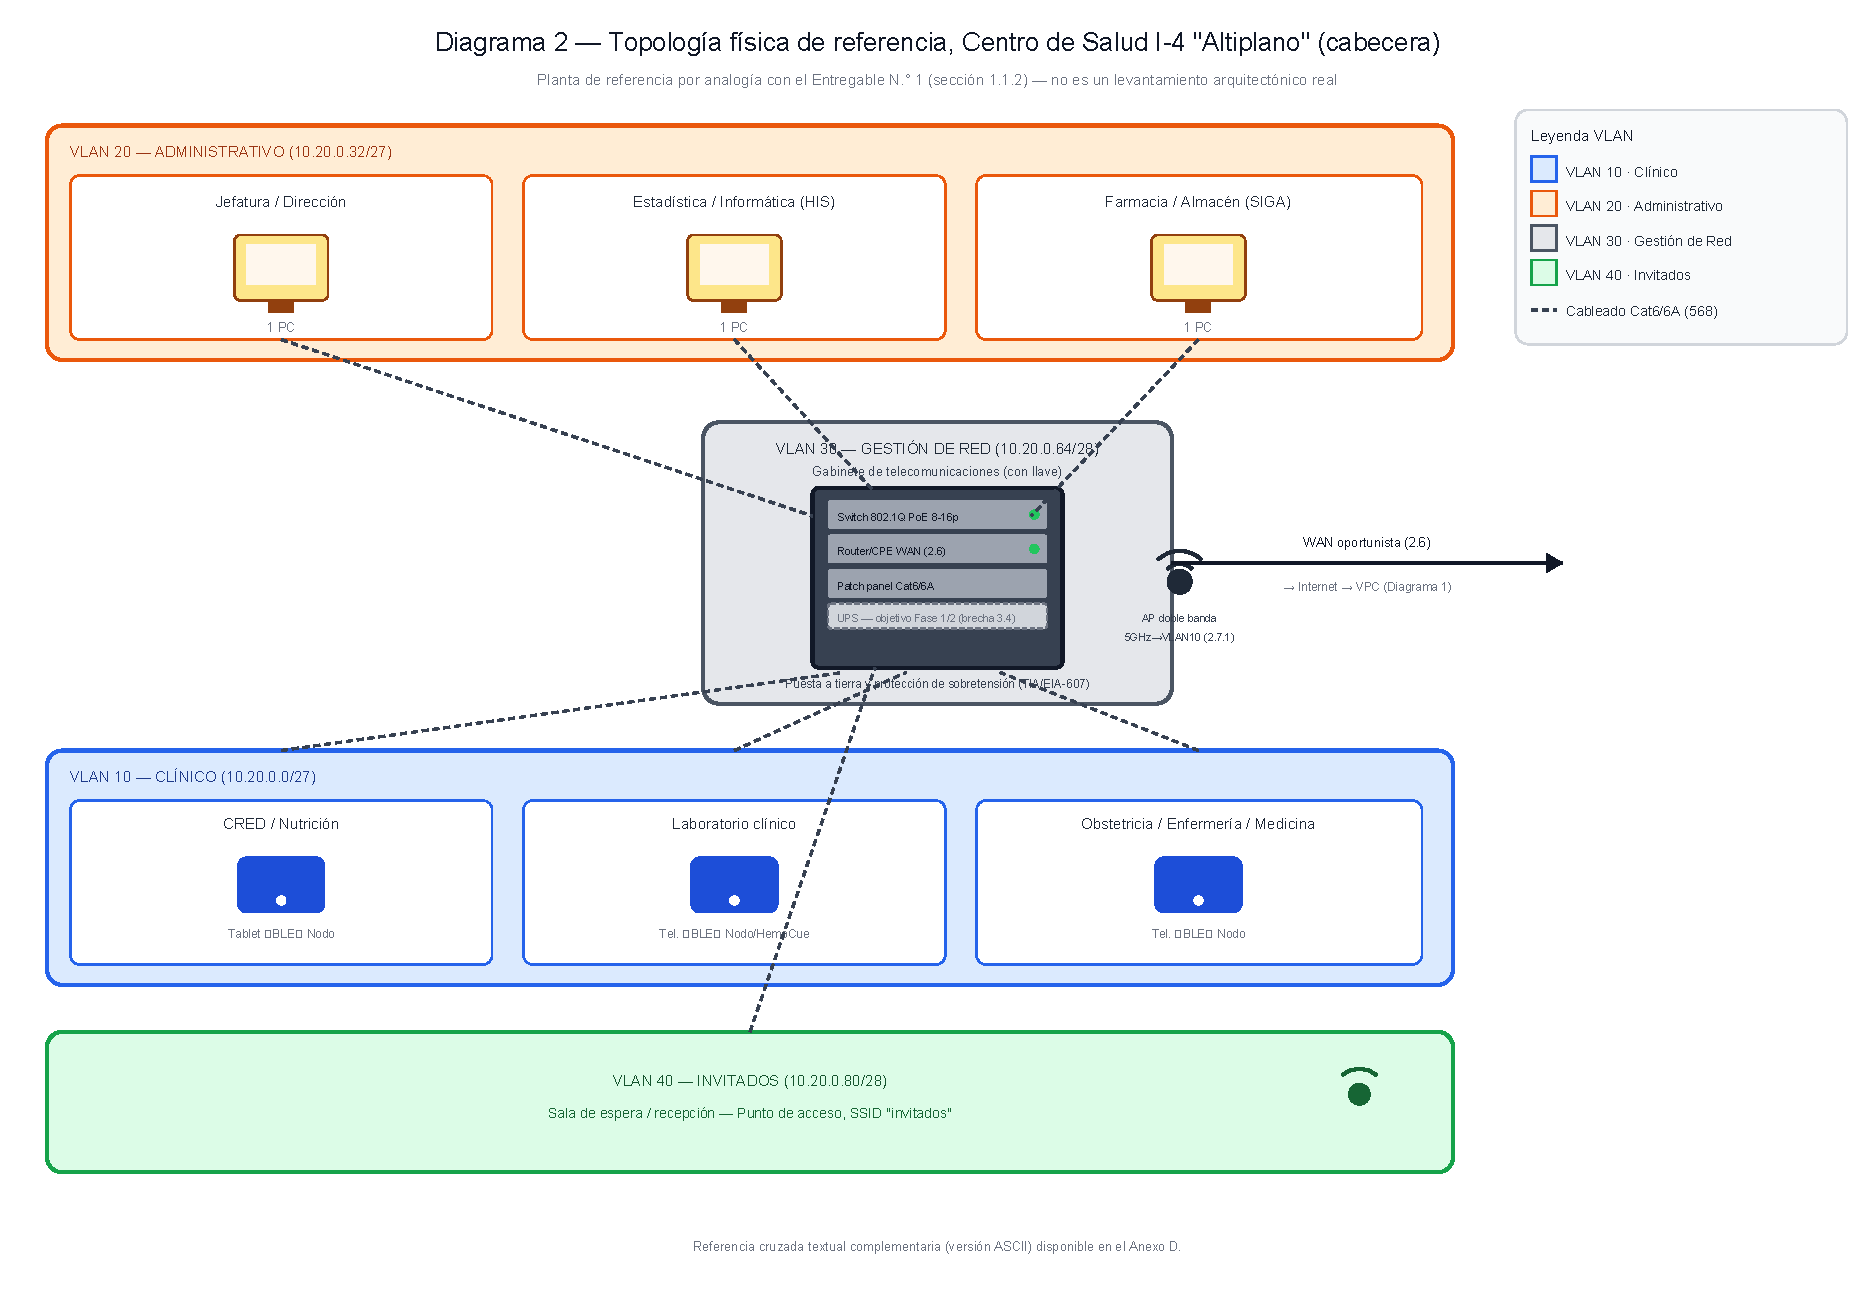
\includegraphics[width=0.88\linewidth,keepaspectratio]{assets/07-diseno-red/diagrama-02-topologia-fisica-cabecera.pdf}}
\caption{Diagrama 2 --- Topología física de referencia, Centro de Salud I-4 ``Altiplano'' (cabecera)}
\end{figure}

\textbf{Diagrama 2 --- Topología física de referencia, Centro de Salud I-4 ``Altiplano'' (cabecera).} Distribución de ambientes por VLAN (10 Clínico, 20 Administrativo, 30 Gestión de Red, 40 Invitados), gabinete de telecomunicaciones central y punto de acceso de doble banda.

Cuatro decisiones de diseño físico se explican a partir de este diagrama. Primero, el \textbf{gabinete de telecomunicaciones se ubica en posición central}, minimizando el cableado horizontal, conforme a la recomendación de TIA/EIA-569 de mantener distancias bajo 90 m (sin ser, a esta escala, un desafío real). Segundo, el gabinete se especifica \textbf{con cierre con llave}, control físico alineado con RNF-06/RNF-07 y con el principio de confidencialidad del Código ACM (sección 4.5). Tercero, se recomienda un \textbf{punto de acceso de doble banda (2.4/5 GHz)} en la zona clínica, priorizando 5 GHz para la VLAN 10 por menor congestión e interferencia con el enlace BLE nodo-teléfono (RQ-RED-12, sección 2.7.1). Cuarto, el punto de acceso de la sala de espera (SSID invitados, VLAN 40) atiende visitas de la DIRESA/GERESA, cooperación o soporte técnico externo, sin exponerlos en ningún momento a la VLAN clínica o administrativa.

\subsection{2.5 Topología física simplificada --- Puestos de Salud I-1/I-2}\label{topologuxeda-fuxedsica-simplificada-puestos-de-salud-i-1i-2}

El \textbf{Diagrama 3}, también producido con herramienta de diagramación vectorial, contrasta deliberadamente con el Diagrama 2 e ilustra por qué \textbf{no se justifica} replicar el esquema completo de 5 VLAN en este tipo de establecimiento: con un único dispositivo con app y un nodo rotativo, una segmentación 802.1Q completa añadiría costo y complejidad de gestión sin un beneficio de seguridad proporcional. La versión ASCII equivalente se conserva en el Anexo D.

\begin{figure}[H]
\centering
\pandocbounded{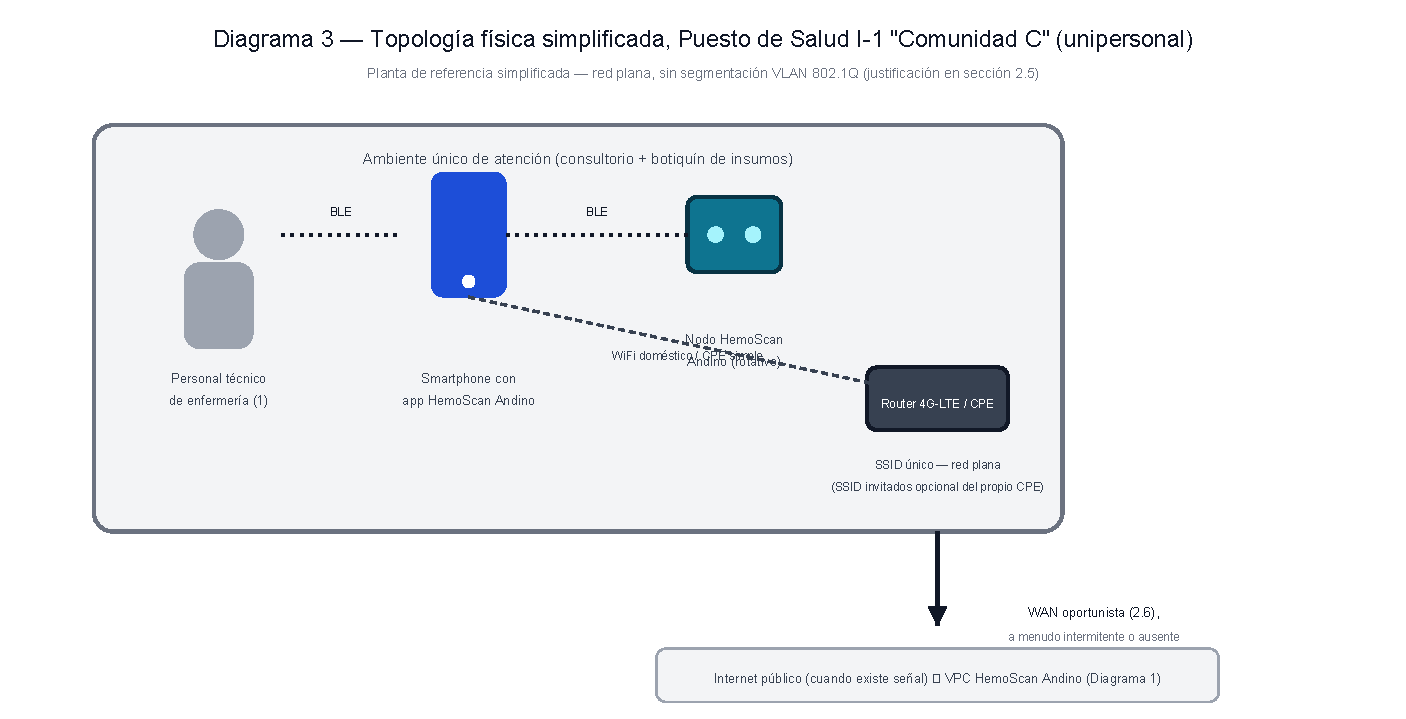
\includegraphics[width=0.88\linewidth,keepaspectratio]{assets/07-diseno-red/diagrama-03-topologia-fisica-puesto-salud.pdf}}
\caption{Diagrama 3 --- Topología física simplificada, Puesto de Salud I-1 ``Comunidad C'' (unipersonal)}
\end{figure}

\textbf{Diagrama 3 --- Topología física simplificada, Puesto de Salud I-1 ``Comunidad C'' (unipersonal).} Red plana sin VLAN 802.1Q; enlace BLE nodo-teléfono y salida WAN oportunista vía CPE doméstico.

Los Puestos de Salud I-2 (2 personas, ``Comunidad A''/``B'') siguen el mismo patrón simplificado, con la diferencia de que el CPE doméstico sirve a dos dispositivos en lugar de uno. Sigue sin justificarse una VLAN 802.1Q dedicada, pero si el propio CPE de bajo costo ofrece ``red de invitados'' integrada (común incluso en routers domésticos económicos), se recomienda activarla como control mínimo de aislamiento cuando personal externo visite el puesto, sin adquirir equipamiento adicional.

\subsection{2.6 Red WAN regional y enlace con la DIRESA}\label{red-wan-regional-y-enlace-con-la-diresa}

El \textbf{Diagrama 4} ilustra la red de área amplia que conecta los 7 establecimientos con el backend en la nube y, a través de este, con la Jefatura de microred, la DIRESA/GERESA y los sistemas nacionales:

\textbf{Diagrama 4 --- Red WAN regional en estrella (postas -\textgreater{} nube -\textgreater{} DIRESA/HIS-MINSA).}

\begin{samepage}\begin{verbatim}
   C.S. I-4 Altiplano        P.S. I-2 "A"/"B"          P.S. I-1 "C/D/E/F"
   (cabecera)                (2 postas)                (4 postas)
        \                         \                          /
         \   HTTPS/TLS, oportunista, sin enlace directo entre postas (RF-19, ADR-01)  /
          \_______________________  ________________________  ______________________/
                                  \/
                         INTERNET PÚBLICO (variable por establecimiento)
                                  |
                                  v
                  VPC HemoScan Andino — Backend FHIR (Diagrama 1, sección 2.2.2)
                                  |
                    +-------------+------------------------------+
                    v             v                              v
        Navegador — Jefatura   Navegador — Analista        Sistemas externos:
        de microred (HTTPS)    DIRESA/GERESA (HTTPS)       HIS-MINSA, Padrón Nominal,
                                                             SIGA (integración diferida, RF-30)
\end{verbatim}\end{samepage}

Un punto merece explicación aparte: el alcance solicitado incluye un ``enlace posta\textless-\textgreater DIRESA''. Del diagrama se desprende que \textbf{no existe un enlace de red dedicado y directo} entre la posta y la DIRESA/GERESA: la Jefatura y el analista acceden a la plataforma web como cualquier cliente de internet, autenticados vía Keycloak (RNF-06), sin VPN site-to-site ni red privada compartida --- consistente con el diagrama de despliegue del Entregable N.° 5 (sección 3.3).

Existe, sin embargo, un segundo significado que sí amerita diseño explícito: el \textbf{canal de interoperabilidad de sistema a sistema} con HIS-MINSA/Padrón Nominal (RF-30), probablemente sujeto a una política propia del MINSA/DIRESA (restricción de IP de origen, VPN dedicada, o un gateway nacional de interoperabilidad) --- \textbf{{[}DATO PENDIENTE DE VALIDAR: mecanismo y política de conectividad exacta exigida por MINSA/DIRESA; no disponible hasta un acercamiento institucional formal{]}}. Se recomienda evaluar en Fase 1 un túnel IPsec site-to-site o una VPN dedicada exclusivamente para este canal, como defensa en profundidad adicional a TLS.

Respecto de las opciones de enlace WAN por posta, en orden de preferencia:

\begin{enumerate}
\def\labelenumi{\arabic{enumi}.}
\tightlist
\item
  \textbf{Primario --- 4G/LTE celular.} Router/CPE con SIM de un operador móvil con cobertura en la zona --- \textbf{{[}DATO PENDIENTE DE VALIDAR: operador y nivel de señal real en la ubicación exacta de cada establecimiento{]}}. Es, en general, la alternativa más económica y de despliegue más simple para zonas rurales altoandinas con alguna cobertura celular.
\item
  \textbf{Secundario/contingencia --- VSAT o servicio satelital de nueva generación} (constelaciones de órbita baja). Alternativa a evaluar para establecimientos sin cobertura celular o como respaldo del enlace primario --- \textbf{{[}DATO PENDIENTE DE VALIDAR: disponibilidad, cobertura y costo real de un proveedor satelital en la ubicación exacta de la microred{]}}.
\item
  \textbf{Última instancia --- sincronización manual (``modo desconectado extendido'').} Cuando ninguna opción anterior esté disponible de forma sostenida, ADR-01 tolera que el personal traslade físicamente el teléfono hacia un punto con señal para vaciar la cola de sincronización; alternativa manual pero arquitectónicamente válida, coherente con la dispersión geográfica diagnosticada (Entregable N.° 1) y con que RF-19/RNF-17 no impongan un límite de tiempo al restablecimiento de la conectividad.
\end{enumerate}

\subsection{2.7 Protocolos y seguridad por segmento}\label{protocolos-y-seguridad-por-segmento}

\subsubsection{2.7.1 Enlace BLE nodo-teléfono}\label{enlace-ble-nodo-teluxe9fono}

El nodo opera como periférico BLE (rol GATT \emph{server}) y el teléfono como central (rol GATT \emph{client}), en relación estrictamente uno a uno por captura, nunca en malla. Ante la ausencia de pantalla o teclado en el ESP32-S3, el mecanismo de emparejamiento más viable es ``Just Works'', que no ofrece protección plena contra ataques de intermediario (MITM); se mitiga mediante controles compensatorios: exigencia de proximidad física real durante el emparejamiento (el propio flujo clínico ya la requiere), ventanas de emparejamiento breves, y el hecho de que el dato transmitido (señales ópticas crudas, sin identificación directa del paciente en el payload BLE) tiene un valor de explotación limitado si fuera interceptado de forma aislada. Se recomienda evaluar, en la siguiente iteración del firmware (paquete EDT 4.3), el uso de \emph{LE Secure Connections} con \emph{bonding} si el stack BLE del ESP32-S3 lo soporta de forma estable --- \textbf{{[}DATO PENDIENTE DE VALIDAR: si el firmware implementará bonding persistente o pairing por sesión; corresponde conjuntamente a los Integrantes 1 y 3{]}}. Para minimizar la interferencia mutua en la banda de 2.4 GHz, se recomienda que el punto de acceso de la VLAN 10 priorice la banda de 5 GHz para el tráfico de la app (sección 2.4), dejando la banda de 2.4 GHz más despejada para el enlace BLE.

\subsubsection{2.7.2 Sincronización app-backend}\label{sincronizaciuxf3n-app-backend}

Toda comunicación entre la app y el backend se realiza mediante HTTPS (TLS 1.2+, RNF-05), con los recursos FHIR transmitidos como \emph{bundles} transaccionales identificados por un UUID generado en el cliente (ADR-01), lo que permite al backend detectar y descartar reintentos duplicados sin perder ninguna determinación clínica. La red no requiere sesiones persistentes ni de baja latencia: cada sincronización es un conjunto de peticiones HTTP POST idempotentes completables en una ventana de conectividad breve e intermitente.

Se recomienda, como buena práctica compatible con el bajo presupuesto de Fase 0, un esquema simple de \textbf{calidad de servicio (QoS)} en el router de la cabecera que priorice el tráfico marcado como clínico (VLAN 10, puerto 443) por encima del de la VLAN 40 (Invitados) en el enlace WAN compartido, mediante marcado DSCP ---funcionalidad habitualmente disponible incluso en routers/CPE de gama baja, sin costo adicional significativo.

\subsubsection{2.7.3 Red LAN/WiFi interna}\label{red-lanwifi-interna}

La red interna de la cabecera opera sobre Ethernet (IEEE 802.3, cableado Cat6/6A) para los puestos fijos y sobre WiFi (IEEE 802.11, doble banda recomendada) para los dispositivos móviles clínicos, con cifrado WPA2-AES como mínimo aceptable y WPA3-Personal como meta, según la compatibilidad del parque de dispositivos de gama baja/media del personal de salud (Restricción 11, Entregable N.° 5). Cada SSID se asocia de forma unívoca a una única VLAN (sección 2.3), evitando el antipatrón de un solo SSID compartido entre perfiles de acceso distintos.

\subsubsection{2.7.4 Diseño para operación offline-first}\label{diseuxf1o-para-operaciuxf3n-offline-first}

Este principio transversal es la contribución de diseño de red más importante del documento: la red de HemoScan Andino \textbf{no está diseñada para eliminar la intermitencia de conectividad rural} (meta poco realista dado el contexto diagnosticado en el Entregable N.° 1), sino para \textbf{convivir con ella sin degradar la función clínica}. Se traduce en tres decisiones ya desarrolladas: (a) ninguna regla de negocio crítica depende de una llamada de red en tiempo real (RF-18, RNF-03); (b) la sincronización se ejecuta de forma oportunista, priorizada y con reintentos exponenciales, nunca bloqueante (RNF-17, ADR-01); y (c) el diseño físico y lógico de la red (secciones 2.1 a 2.6) reserva la dependencia de conectividad continua exclusivamente para las funciones no críticas (dashboard web, reportes agregados, interoperabilidad externa).

\begin{center}\rule{0.5\linewidth}{0.5pt}\end{center}

\section{3. Incorporación de Redundancia}\label{incorporaciuxf3n-de-redundancia}

\subsection{3.1 Análisis de puntos únicos de falla (SPOF)}\label{anuxe1lisis-de-puntos-uxfanicos-de-falla-spof}

La siguiente tabla identifica los puntos únicos de falla (\emph{Single Point of Failure}) de la red, su modo de falla, impacto, probabilidad cualitativa en Fase 0, y el nivel de redundancia efectivamente alcanzable hoy frente al objetivo de fases futuras. Es, deliberadamente, el punto del documento donde se declara con mayor honestidad la brecha entre lo deseable y lo presupuestalmente viable --- con una única excepción real ya incorporada, detallada en la fila de enlace WAN de la cabecera.

{\small
\begin{longtable}[]{@{}
  >{\raggedright\arraybackslash}p{(\linewidth - 12\tabcolsep) * \real{0.1429}}
  >{\raggedright\arraybackslash}p{(\linewidth - 12\tabcolsep) * \real{0.1429}}
  >{\raggedright\arraybackslash}p{(\linewidth - 12\tabcolsep) * \real{0.1429}}
  >{\raggedright\arraybackslash}p{(\linewidth - 12\tabcolsep) * \real{0.1429}}
  >{\raggedright\arraybackslash}p{(\linewidth - 12\tabcolsep) * \real{0.1429}}
  >{\raggedright\arraybackslash}p{(\linewidth - 12\tabcolsep) * \real{0.1429}}
  >{\raggedright\arraybackslash}p{(\linewidth - 12\tabcolsep) * \real{0.1429}}@{}}
\toprule\noalign{}
\begin{minipage}[b]{\linewidth}\raggedright
Componente
\end{minipage} & \begin{minipage}[b]{\linewidth}\raggedright
Modo de falla
\end{minipage} & \begin{minipage}[b]{\linewidth}\raggedright
Impacto
\end{minipage} & \begin{minipage}[b]{\linewidth}\raggedright
Probabilidad (Fase 0)
\end{minipage} & \begin{minipage}[b]{\linewidth}\raggedright
Mitigación aplicada en Fase 0
\end{minipage} & \begin{minipage}[b]{\linewidth}\raggedright
Redundancia Fase 0
\end{minipage} & \begin{minipage}[b]{\linewidth}\raggedright
Redundancia objetivo Fase 1/2
\end{minipage} \\
\midrule\noalign{}
\endhead
\bottomrule\noalign{}
\endlastfoot
Servidor único (backend + BD + Keycloak) & Caída de instancia, saturación de recursos, corrupción de base de datos & Bloquea sincronización, dashboard web y autenticación de sesiones nuevas; \textbf{no afecta} la captura/tamizaje offline (RNF-03) & Media (proveedor de nube de bajo costo, sin SLA contratado --- RNF-20 pendiente) & Respaldo automatizado diario de base de datos (sección 3.3) & Ninguna (instancia única) --- \textbf{riesgo residual aceptado explícitamente} & Instancia secundaria en espera (\emph{warm standby}) o servicio gestionado multi-zona \\
Enlace WAN --- cabecera & Corte de señal celular, saturación de la torre & Bloquea sincronización y acceso web; \textbf{no bloquea} captura/tamizaje (offline-first) & Alta (zona rural altoandina --- Debilidad D2) & \textbf{Router/CPE con doble SIM de dos operadores distintos (Anexo E, \textasciitilde=S/ 450) con conmutación automática} --- única medida de redundancia física de Fase 0 efectivamente presupuestada, condicionada al cierre de la brecha de financiamiento declarada en 3.4 & \textbf{Parcial} (dual-operador en un único router; sin diversidad de router físico) & Router dual con dos módems físicos independientes, o segundo enlace satelital \\
Enlace WAN --- puestos de salud I-1/I-2 & Corte de señal celular, saturación de la torre & Bloquea sincronización y acceso web; \textbf{no bloquea} captura (offline-first) & Alta (Debilidad D2) & Cola de reintentos exponenciales (RNF-17, ADR-01); operación offline \textgreater= 72 h (RNF-03) & Ninguna --- un solo proveedor/tecnología, por no justificarse el costo de un CPE dual-SIM en establecimientos de 1-2 dispositivos & Evaluar dual-SIM solo si el costo unitario baja en Fase 1/2 \\
Suministro eléctrico de la posta & Corte de energía, frecuente en zona altoandina & Apaga router/AP/switch; interrumpe el ciclo de captura si el nodo/teléfono se descargan & Alta (Debilidad D2) & Buffer local del nodo (RF-05, \textgreater= 50 capturas) y batería propia del teléfono & Sin UPS presupuestado (brecha declarada, sección 3.4) & UPS de 30-60 min mínimo para el equipo de red crítico de la cabecera \\
Switch/AP de la cabecera & Falla de hardware, sobrecalentamiento & Pérdida de LAN/WiFi interna en la cabecera & Baja-Media & Ninguna (equipo único); reemplazo manual reactivo & Ninguna & Equipo de repuesto en almacén (\emph{cold spare}) o AP secundario con solapamiento de cobertura \\
Nodo HemoScan Andino (hardware) & Falla de sensor, de batería o del módulo BLE & Imposibilidad de captura en el punto de atención específico & Media (3 nodos totales, sin unidad de respaldo dedicada por establecimiento) & Rotación operativa de los 3 nodos entre brigadas (EDT 2.4/2.5); el buffer local no se pierde ante el cambio de nodo & Parcial (rotación operativa, no redundancia técnica 1:1) & Un nodo de respaldo adicional por microred activa en Fase 1 \\
Acceso web de la Jefatura/DIRESA & Corte de internet en cualquiera de los dos extremos & Imposibilidad de consulta en tiempo real del dashboard/mapa de cobertura & Media-Alta & Reportes exportables en PDF/CSV como canal alterno asíncrono (RF-36) & Sin alternativa en tiempo real & Posible acuerdo de conectividad reforzada con DIRESA en Fase 1/2 \\
\end{longtable}
}

\subsection{3.2 Alta disponibilidad por capas}\label{alta-disponibilidad-por-capas}

La siguiente tabla desagrega la estrategia de alta disponibilidad por capa, con objetivos ilustrativos de \textbf{RPO} y \textbf{RTO}, explícitamente etiquetados como metas de diseño y no como compromisos contractuales de un SLA (RNF-20 sigue pendiente de validar):

{\small
\begin{longtable}[]{@{}
  >{\raggedright\arraybackslash}p{(\linewidth - 8\tabcolsep) * \real{0.2000}}
  >{\raggedright\arraybackslash}p{(\linewidth - 8\tabcolsep) * \real{0.2000}}
  >{\raggedright\arraybackslash}p{(\linewidth - 8\tabcolsep) * \real{0.2000}}
  >{\raggedright\arraybackslash}p{(\linewidth - 8\tabcolsep) * \real{0.2000}}
  >{\raggedright\arraybackslash}p{(\linewidth - 8\tabcolsep) * \real{0.2000}}@{}}
\toprule\noalign{}
\begin{minipage}[b]{\linewidth}\raggedright
Capa
\end{minipage} & \begin{minipage}[b]{\linewidth}\raggedright
Estrategia de alta disponibilidad (Fase 0)
\end{minipage} & \begin{minipage}[b]{\linewidth}\raggedright
RPO ilustrativo
\end{minipage} & \begin{minipage}[b]{\linewidth}\raggedright
RTO ilustrativo
\end{minipage} & \begin{minipage}[b]{\linewidth}\raggedright
Estrategia objetivo (Fase 1/2)
\end{minipage} \\
\midrule\noalign{}
\endhead
\bottomrule\noalign{}
\endlastfoot
Cliente (app móvil) & Local-first + \emph{outbox} (ADR-01): el dispositivo es la fuente de verdad hasta la sincronización & 0 (no hay pérdida: los datos persisten localmente) & No aplica --- la app sigue plenamente operativa sin el servidor & Se mantiene igual; es el patrón más maduro de todo el diseño \\
Red LAN/WiFi (cabecera) & Un único punto de acceso, ubicación central & No aplica & Horas (reemplazo manual) & Segundo AP con solapamiento de cobertura \\
Red WAN --- cabecera & Router dual-SIM (dos operadores), conmutación automática (Anexo E) & Segundos a minutos (conmutación entre SIM) & Minutos, sujeto a la cobertura del operador secundario & Router dual con dos módems físicos independientes \\
Red WAN --- puestos I-1/I-2 & Un único enlace (4G u otro, según validación de campo) + cola de reintentos & Hasta 72 h de operación offline tolerada (RNF-03) & Depende del restablecimiento del operador (fuera de control del equipo) & Enlace dual (\emph{multi-WAN}) si el costo lo permite \\
Servidor (backend + BD + Keycloak) & Instancia única + respaldo diario automatizado & Hasta 24 h (ventana ilustrativa entre respaldos) & Hasta 48 h (tiempo ilustrativo de restauración manual) & Instancia secundaria o servicio gestionado multi-zona \\
\end{longtable}
}

El \textbf{Diagrama 5} resume estas rutas de redundancia y contingencia, distinguiendo lo que existe en Fase 0 de lo que es objetivo de fases posteriores:

\textbf{Diagrama 5 --- Rutas de redundancia y failover (Fase 0 vigente vs.~objetivo Fase 1/2).}

\begin{samepage}\begin{verbatim}
Cliente (app móvil)
  +- Ruta primaria (Fase 0): WiFi de la posta -> Internet -> Backend (nube)
  +- Ruta de contingencia (Fase 0, si aplica): datos móviles propios del teléfono del
  |  personal de salud, cuando exista SIM personal disponible -> Internet -> Backend
  +- Ruta última (Fase 0, siempre disponible): operación 100 % offline hasta 72 h
     continuas (RNF-03) + sincronización manual al desplazarse a un punto con señal

Posta — cabecera (router/CPE)
  +- Ruta primaria (Fase 0): Operador A vía SIM 1 del router dual-SIM (Anexo E)
  +- Ruta secundaria (Fase 0, conmutación automática): Operador B vía SIM 2 del mismo
     router — [DATO PENDIENTE DE VALIDAR: cierre de la brecha de financiamiento, sección 3.4]

Posta — puestos I-1/I-2 (router/CPE)
  +- Ruta primaria (Fase 0): un solo operador 4G/LTE — [DATO PENDIENTE DE VALIDAR: operador]
  +- Ruta objetivo (Fase 1/2): segundo operador o enlace satelital, router multi-WAN

Servidor (nube)
  +- Ruta primaria (Fase 0): instancia única + respaldo diario (sección 3.3)
  +- Ruta objetivo (Fase 1/2): instancia secundaria o servicio gestionado
     multi-zona, con conmutación por balanceador o DNS de failover
\end{verbatim}\end{samepage}

\subsection{3.3 Plan de contingencia y recuperación ante desastres}\label{plan-de-contingencia-y-recuperaciuxf3n-ante-desastres}

Se documenta a continuación un plan de contingencia básico (\emph{runbook}), suficiente para el alcance de la Fase 0, con escenario, mecanismo de detección, respuesta inmediata y responsable:

{\small
\begin{longtable}[]{@{}
  >{\raggedright\arraybackslash}p{(\linewidth - 8\tabcolsep) * \real{0.2000}}
  >{\raggedright\arraybackslash}p{(\linewidth - 8\tabcolsep) * \real{0.2000}}
  >{\raggedright\arraybackslash}p{(\linewidth - 8\tabcolsep) * \real{0.2000}}
  >{\raggedright\arraybackslash}p{(\linewidth - 8\tabcolsep) * \real{0.2000}}
  >{\raggedright\arraybackslash}p{(\linewidth - 8\tabcolsep) * \real{0.2000}}@{}}
\toprule\noalign{}
\begin{minipage}[b]{\linewidth}\raggedright
Escenario
\end{minipage} & \begin{minipage}[b]{\linewidth}\raggedright
Detección
\end{minipage} & \begin{minipage}[b]{\linewidth}\raggedright
Respuesta inmediata
\end{minipage} & \begin{minipage}[b]{\linewidth}\raggedright
Responsable
\end{minipage} & \begin{minipage}[b]{\linewidth}\raggedright
Referencia cruzada
\end{minipage} \\
\midrule\noalign{}
\endhead
\bottomrule\noalign{}
\endlastfoot
Corte de energía en la posta & Reporte del personal / pérdida de señal del AP & Continuar el tamizaje con la batería del teléfono/nodo; posponer la sincronización & Personal de salud / Integrante 1 (soporte remoto) & RF-18, RNF-03; EDT 2.5 \\
Caída del enlace WAN & La cola de sincronización agota reintentos sin conectar & La app continúa operando offline; reintento automático con retroceso exponencial & App móvil (automático); Integrante 1 (diagnóstico si es prolongado) & RNF-17, ADR-01 \\
Caída del servidor/backend & Verificación de disponibilidad (\emph{healthcheck} HTTP) o reporte de la Jefatura sobre imposibilidad de acceder al dashboard & Ejecutar el procedimiento de reinicio de la instancia; restaurar desde el respaldo más reciente si es necesario & Integrante 1 & EDT 2.2; sección 3.1 \\
Falla de un nodo de hardware & El personal reporta que el nodo no enciende o no logra emparejarse & Rotar hacia uno de los otros 2 nodos disponibles (EDT 2.4/2.5); registrar la incidencia en la bitácora de campo & Personal de salud / Integrante 1 & EDT 2.5 (bitácora de incidencias, disponibilidad \textgreater= 90 \% de las jornadas de campo) \\
Sospecha de incidente de seguridad (acceso no autorizado) & Alerta del propio Keycloak o revisión de los recursos AuditEvent & Revocar credenciales comprometidas; revisar trazas de auditoría; notificar conforme al protocolo de la Ley N.° 29733 & Integrante 1 (técnico) / Integrante 2 (gestión y comunicación) & RNF-06, RNF-07, RF-31, RN-11 \\
\end{longtable}
}

La política de respaldo de Fase 0 consiste en una copia automatizada diaria de PostgreSQL/PostGIS hacia un almacenamiento distinto al de la instancia primaria, retenida un mínimo razonable de 30 días --- \textbf{{[}DATO PENDIENTE DE VALIDAR: política exacta de retención y mecanismo de respaldo del proveedor de nube finalmente elegido{]}}. Es modesta frente a un esquema activo-activo, pero consistente con el riesgo aceptado en 3.1 y con que ninguna función clínica crítica dependa de la disponibilidad continua del servidor.

\subsection{3.4 Brecha presupuestal de redundancia y hoja de ruta por fases}\label{brecha-presupuestal-de-redundancia-y-hoja-de-ruta-por-fases}

El presupuesto validado de Fase 0 (S/ 3,124) no contiene una partida específica para equipamiento de red más allá del rubro ``servidor/nube'' (S/ 320, EDT 2.2). Frente a esta restricción, el equipo adopta una única medida correctiva concreta y presupuestada dentro de la propia estimación referencial del Anexo E: el \textbf{router/CPE 4G-LTE con doble SIM} (\textasciitilde=S/ 450) se recomienda como el equipo WAN de la cabecera desde la propia Fase 0 ---y no como un ítem diferido a Fase 1/2, como se planteaba en una versión anterior de este documento---, porque el sobrecosto frente a un router de SIM única (\textasciitilde=S/ 200-250) es marginal y porque, de todas las capas analizadas en 3.1, es la que ofrece la relación costo-beneficio de redundancia más alta.

Ese ítem, sin embargo, \textbf{no está cerrado financieramente}: la partida de contingencia del 10 \% del presupuesto validado (S/ 284) no cubre el costo íntegro de S/ 450, dejando un diferencial de aproximadamente \textbf{S/ 166} --- \textbf{{[}DATO PENDIENTE DE VALIDAR: fuente de financiamiento del diferencial; opciones no excluyentes son un aporte de contraparte de la microred/DIRESA anfitriona, una reasignación menor dentro de la línea base del Entregable N.° 3, o una ampliación presupuestal formal{]}}. Hasta que ese diferencial se cierre, la redundancia de enlace WAN de la cabecera se mantiene como una recomendación de diseño fuertemente respaldada, no como una redundancia ya garantizada --- distinción que la tabla 3.1 refleja explícitamente.

El resto del equipamiento del Anexo E (switch, puntos de acceso, cableado, UPS; \textasciitilde=S/ 1,280 adicionales) permanece sin fuente de financiamiento identificada. La hoja de ruta de cierre de esa brecha mayor sigue siendo la proyección de hosting de Fase 1 (\textasciitilde=S/ 1,200/año, Entregable N.° 2), que ya contempla un salto de escala coherente con presupuestar entonces un proveedor de nube multi-zona y el equipamiento de red hoy pendiente.

\begin{center}\rule{0.5\linewidth}{0.5pt}\end{center}

\section{4. Cumplimiento de Estándares}\label{cumplimiento-de-estuxe1ndares}

\subsection{4.1 Estándares de cableado estructurado}\label{estuxe1ndares-de-cableado-estructurado}

{\small
\begin{longtable}[]{@{}
  >{\raggedright\arraybackslash}p{(\linewidth - 4\tabcolsep) * \real{0.3333}}
  >{\raggedright\arraybackslash}p{(\linewidth - 4\tabcolsep) * \real{0.3333}}
  >{\raggedright\arraybackslash}p{(\linewidth - 4\tabcolsep) * \real{0.3333}}@{}}
\toprule\noalign{}
\begin{minipage}[b]{\linewidth}\raggedright
Estándar
\end{minipage} & \begin{minipage}[b]{\linewidth}\raggedright
Ámbito
\end{minipage} & \begin{minipage}[b]{\linewidth}\raggedright
Aplicación en el diseño de HemoScan Andino
\end{minipage} \\
\midrule\noalign{}
\endhead
\bottomrule\noalign{}
\endlastfoot
TIA/EIA-568-C (series) / ISO/IEC 11801 & Cableado de telecomunicaciones para edificios comerciales & Cableado horizontal Cat6/Cat6A recomendado para la cabecera (Diagrama 2), con margen de desempeño para un eventual salto a mayores velocidades en Fase 2; conectorización RJ-45 bajo esquema T568B \\
TIA/EIA-569-D & Rutas y espacios para telecomunicaciones & Gabinete de telecomunicaciones de pequeño formato en la cabecera, canalización protegida frente a polvo/humedad, y distancias de cableado horizontal dentro del límite convencional de 90 m \\
TIA/EIA-606-B & Administración de la infraestructura de telecomunicaciones (etiquetado y documentación) & Esquema de etiquetado propuesto para puertos de switch, cables y VLAN, con convención {[}Sitio{]}-{[}Ambiente{]}-{[}Consecutivo{]} y ejemplo aplicado al patch panel de la cabecera (Anexo D), que permite a cualquier técnico de soporte ---incluyendo personal nuevo, dada la alta rotación por el régimen SERUMS diagnosticada en el Entregable N.° 1--- identificar sin ambigüedad cualquier punto de la red \\
TIA/EIA-607-D & Puesta a tierra y enlace equipotencial & Puesta a tierra del gabinete y protección contra sobretensión, dado el riesgo de tormentas eléctricas del altiplano a 3,800 m s. n.~m. y la inestabilidad eléctrica ya diagnosticada (Debilidad D2) \\
TIA-942 (referencia parcial) & Infraestructura de centros de datos & No aplica directamente en Fase 0, al alojarse el backend en un proveedor de nube pública; se cita como referencia solo si una fase futura contemplara un centro de datos propio o de la DIRESA \\
\end{longtable}
}

\subsection{4.2 Estándares IEEE 802.x}\label{estuxe1ndares-ieee-802.x}

{\small
\begin{longtable}[]{@{}
  >{\raggedright\arraybackslash}p{(\linewidth - 6\tabcolsep) * \real{0.2500}}
  >{\raggedright\arraybackslash}p{(\linewidth - 6\tabcolsep) * \real{0.2500}}
  >{\raggedright\arraybackslash}p{(\linewidth - 6\tabcolsep) * \real{0.2500}}
  >{\raggedright\arraybackslash}p{(\linewidth - 6\tabcolsep) * \real{0.2500}}@{}}
\toprule\noalign{}
\begin{minipage}[b]{\linewidth}\raggedright
Estándar
\end{minipage} & \begin{minipage}[b]{\linewidth}\raggedright
Ámbito
\end{minipage} & \begin{minipage}[b]{\linewidth}\raggedright
Aplicación específica en HemoScan Andino
\end{minipage} & \begin{minipage}[b]{\linewidth}\raggedright
Elemento(s) de red
\end{minipage} \\
\midrule\noalign{}
\endhead
\bottomrule\noalign{}
\endlastfoot
IEEE 802.3 / 802.3u / 802.3ab (Ethernet, Fast Ethernet, Gigabit sobre par trenzado) & Cableado LAN & Backbone y cableado horizontal de la cabecera; puertos de switch a 1000 Mbps como mínimo recomendado & Switch, patch panel, cableado horizontal (Diagrama 2) \\
IEEE 802.3af (PoE) / 802.3at (PoE+) & Alimentación eléctrica sobre Ethernet & Alimentación de los puntos de acceso WiFi desde un switch, mitigando parcialmente los cortes eléctricos frecuentes (Debilidad D2) sin tendido eléctrico adicional & Switch PoE, puntos de acceso \\
IEEE 802.11 (WiFi), en particular 802.11n/ac de doble banda & Red inalámbrica local & SSID mapeados 1:1 a las VLAN 10/20/30/40 de la cabecera (sección 2.3); banda de 5 GHz priorizada para tráfico clínico (sección 2.7.1) & Puntos de acceso, dispositivos móviles/tablets \\
IEEE 802.1Q & Etiquetado de VLAN (\emph{trunking}) & Enlace troncal switch\textless-\textgreater router/firewall que transporta las 5 VLAN de la cabecera sobre un único enlace físico & Switch, router/firewall \\
IEEE 802.1X & Control de acceso a la red basado en puertos (NAC) & Recomendado para la VLAN 20 en Fase 1/2, integrado conceptualmente con Keycloak (ADR-09); en Fase 0 se acepta un control más simple (filtrado por MAC/contraseña robusta) por restricción de presupuesto --- \textbf{brecha declarada explícitamente} & Switch, controlador de acceso \\
IEEE 802.1D (STP) / 802.1w (RSTP) & Prevención de bucles de capa 2 & Aplicable si la cabecera incorpora un segundo switch en Fase 1/2 (sección 3.2); no requerido con el switch único de Fase 0 & Switches (topología con más de un nodo de capa 2) \\
IEEE 802.11i (WPA2) / WPA3 & Seguridad de la capa de enlace inalámbrica & Cifrado obligatorio en las 4 VLAN inalámbricas de la cabecera; WPA3-Personal como meta, WPA2-AES como mínimo aceptable dado el parque de dispositivos de gama baja/media & Puntos de acceso, dispositivos móviles \\
Familia IEEE 802.15 (WPAN) --- referencia histórica de Bluetooth & Redes de área personal inalámbricas & El enlace nodo\textless-\textgreater teléfono opera sobre BLE, hoy gobernado por el Bluetooth SIG y no por el IEEE, aunque originado dentro de la familia WPAN 802.15; se cita por completitud, no como certificación IEEE vigente sobre BLE & Nodo HemoScan Andino, módulo BLE del teléfono \\
\end{longtable}
}

\subsection{4.3 Cumplimiento normativo sectorial}\label{cumplimiento-normativo-sectorial}

{\small
\begin{longtable}[]{@{}
  >{\raggedright\arraybackslash}p{(\linewidth - 4\tabcolsep) * \real{0.3333}}
  >{\raggedright\arraybackslash}p{(\linewidth - 4\tabcolsep) * \real{0.3333}}
  >{\raggedright\arraybackslash}p{(\linewidth - 4\tabcolsep) * \real{0.3333}}@{}}
\toprule\noalign{}
\begin{minipage}[b]{\linewidth}\raggedright
Norma
\end{minipage} & \begin{minipage}[b]{\linewidth}\raggedright
Exigencia relevante para la red
\end{minipage} & \begin{minipage}[b]{\linewidth}\raggedright
Control de red aplicado
\end{minipage} \\
\midrule\noalign{}
\endhead
\bottomrule\noalign{}
\endlastfoot
Ley N.° 29733 (Protección de Datos Personales) & Minimización, seguridad y confidencialidad de datos de salud de menores de edad (RNF-07, RNF-19) & Segmentación VLAN 10 Clínico aislada de VLAN 40 Invitados y VLAN 20 Administrativo (sección 2.3); cifrado TLS 1.2+ en tránsito (RNF-05); acceso administrativo restringido a VLAN 20/30 \\
DS 115-2025-PCM (reglamento de IA, Ley N.° 31814) & Trazabilidad y supervisión humana de sistemas de IA en salud; registro auditable de toda inferencia (RNF-08, RNF-18) & Sincronización horaria (NTP) obligatoria en todos los puntos de captura y registro (sección 4.3.1); disponibilidad suficiente para no bloquear la auditoría posterior, sin comprometer la operación offline crítica \\
NTS 213-MINSA/DGIESP-2024 & Continuidad del proceso de tamizaje y consejería (no impone requisitos de red directos) & Diseño offline-first que no condiciona la atención clínica a la disponibilidad de conectividad (sección 2.7.4) \\
OSIPTEL (regulación peruana de telecomunicaciones) & Uso del espectro radioeléctrico & WiFi (802.11) y BLE (2.4 GHz) operan en bandas no licenciadas; no se requiere trámite ante OSIPTEL. El enlace 4G/LTE opera bajo el espectro licenciado del operador contratado como servicio, sin trámite propio de HemoScan Andino \\
\end{longtable}
}

\subsubsection{4.3.1 Sincronización horaria (NTP) como requisito silencioso de auditabilidad}\label{sincronizaciuxf3n-horaria-ntp-como-requisito-silencioso-de-auditabilidad}

Se destaca un requisito fácil de omitir pero indispensable para el DS 115-2025-PCM: la integridad de los recursos FHIR Provenance/AuditEvent (RF-31, RNF-08) depende de que las marcas de tiempo del nodo, el teléfono y el backend sean \textbf{consistentes entre sí}. Si los relojes se desincronizan (escenario plausible en dispositivos de gama baja/media sin mantenimiento regular), la secuencia auditable de ``qué ocurrió primero'' ---captura, inferencia, corrección por altitud, confirmación clínica--- podría volverse ambigua, debilitando exactamente la trazabilidad exigida. Se recomienda que el backend en la nube ejecute un cliente NTP estándar sincronizado contra servidores de tiempo confiables, y que la app móvil registre, junto a cada marca de tiempo local, un indicador de la última sincronización horaria conocida del dispositivo, de modo que cualquier inconsistencia temporal sea, en sí misma, detectable y auditable en lugar de silenciosa.

\subsection{4.4 Matriz consolidada de cumplimiento}\label{matriz-consolidada-de-cumplimiento}

{\small
\begin{longtable}[]{@{}
  >{\raggedright\arraybackslash}p{(\linewidth - 4\tabcolsep) * \real{0.3333}}
  >{\raggedright\arraybackslash}p{(\linewidth - 4\tabcolsep) * \real{0.3333}}
  >{\raggedright\arraybackslash}p{(\linewidth - 4\tabcolsep) * \real{0.3333}}@{}}
\toprule\noalign{}
\begin{minipage}[b]{\linewidth}\raggedright
Dimensión de cumplimiento
\end{minipage} & \begin{minipage}[b]{\linewidth}\raggedright
Estado en este diseño
\end{minipage} & \begin{minipage}[b]{\linewidth}\raggedright
Observación
\end{minipage} \\
\midrule\noalign{}
\endhead
\bottomrule\noalign{}
\endlastfoot
Cableado estructurado (TIA/EIA-568/569/606/607, ISO/IEC 11801) & Aplicado como diseño de referencia & Pendiente de validación con relevamiento de campo real \\
Redes de área local y personal (IEEE 802.3, 802.11, 802.15) & Aplicado & BLE gobernado hoy por Bluetooth SIG, no por IEEE (aclaración explícita en 4.2) \\
Segmentación y control de acceso (802.1Q, 802.1X) & 802.1Q aplicado plenamente; 802.1X diferido a Fase 1/2 & Brecha declarada explícitamente por restricción de presupuesto/capacidades de Fase 0 \\
Protección de datos personales (Ley N.° 29733) & Aplicado mediante segmentación, cifrado y control de acceso & Pendiente de dictamen de un comité de ética constituido (Entregable N.° 1) \\
Marco de IA en salud (DS 115-2025-PCM) & Aplicado mediante NTP, disponibilidad y no bloqueo de la supervisión humana & La responsabilidad principal de la trazabilidad de IA recae en el software (Entregable N.° 5); la red la habilita, no la reemplaza \\
Regulación de telecomunicaciones (OSIPTEL) & Cumplido por uso de bandas no licenciadas y de espectro licenciado de operador contratado & No se identifican trámites regulatorios propios pendientes para HemoScan Andino como organización \\
\end{longtable}
}

\subsection{4.5 Ética profesional en el diseño de red (Código de Ética y Conducta Profesional de la ACM)}\label{uxe9tica-profesional-en-el-diseuxf1o-de-red-cuxf3digo-de-uxe9tica-y-conducta-profesional-de-la-acm}

El diseño de una red que transporta datos de salud de menores de edad en un contexto de vulnerabilidad social y geográfica admite una lectura desde la ética profesional de la disciplina, para lo cual se adopta como referencia el \textbf{Código de Ética y Conducta Profesional de la ACM (2018)}. El principio \textbf{1.2 (``Evitar daño'')} se traduce en la segmentación VLAN que impide que un dispositivo de invitado comprometido alcance datos clínicos (sección 2.3), y en la declaración explícita ---no ocultamiento--- de los riesgos residuales de la Fase 0 (servidor único, ausencia de UPS, redundancia WAN condicionada a financiamiento) en la sección 3.1. El principio \textbf{1.6 (``Respetar la privacidad'')} se materializa en el aislamiento de la VLAN clínica y en la reserva de un segmento propio para el futuro canal de aprendizaje federado que nunca debe transportar datos crudos de pacientes (RN-09, sección 2.2.2). El principio \textbf{1.7 (``Honrar la confidencialidad'')} respalda el control de acceso físico al gabinete de telecomunicaciones (sección 2.4, Anexo D) y la restricción de la VLAN 30 a personal técnico autorizado.

El principio \textbf{2.5 (``Ofrecer evaluaciones exhaustivas de los sistemas informáticos y sus impactos, incluido el análisis de riesgos posibles'')} es, en esencia, el mandato que la sección 3 intenta cumplir: un análisis de puntos únicos de falla que no minimiza ni exagera el riesgo real de una arquitectura de Fase 0 deliberadamente austera. Se añade el principio \textbf{3.7 (``Reconocer y prestar especial atención a los sistemas que se integran en la infraestructura de la sociedad'')}: si HemoScan Andino avanza hacia la Fase 2 de escalamiento regional (Entregable N.° 2), su red dejará progresivamente de ser un proyecto de tesis para convertirse en infraestructura crítica de salud pública regional, responsabilidad que este diseño anticipa desde la Fase 0 mediante la escalabilidad del direccionamiento (sección 2.2) y la hoja de ruta de redundancia (sección 3.4), en lugar de postergarla para cuando la escala haga más costoso corregirla.

\begin{center}\rule{0.5\linewidth}{0.5pt}\end{center}

\section{Anexos}\label{anexos}

\subsection{Anexo A --- Glosario de términos técnicos de este entregable}\label{anexo-a-glosario-de-tuxe9rminos-tuxe9cnicos-de-este-entregable}

{\small
\begin{longtable}[]{@{}
  >{\raggedright\arraybackslash}p{(\linewidth - 2\tabcolsep) * \real{0.5000}}
  >{\raggedright\arraybackslash}p{(\linewidth - 2\tabcolsep) * \real{0.5000}}@{}}
\toprule\noalign{}
\begin{minipage}[b]{\linewidth}\raggedright
Término
\end{minipage} & \begin{minipage}[b]{\linewidth}\raggedright
Definición breve
\end{minipage} \\
\midrule\noalign{}
\endhead
\bottomrule\noalign{}
\endlastfoot
ACL (Access Control List) & Lista de control de acceso; conjunto de reglas que permiten o deniegan tráfico entre segmentos de red (sección 2.3) \\
BLE / GATT & Bluetooth Low Energy y su perfil de atributos genéricos (\emph{Generic Attribute Profile}), usado en el enlace nodo-teléfono \\
CIDR (Classless Inter-Domain Routing) & Notación de direccionamiento IP sin clases, usada para expresar subredes (p.~ej., /24, /27) \\
CPE (Customer Premises Equipment) & Equipo de telecomunicaciones instalado en las instalaciones del cliente (router/módem de la posta) \\
DMZ (Zona Desmilitarizada) & Segmento de red perimetral que aísla los recursos expuestos a internet de la red interna; reinterpretada en este documento como subred pública/privada de una VPC (sección 2.2.2) \\
DSCP & \emph{Differentiated Services Code Point}; campo usado para marcar y priorizar tráfico (calidad de servicio, sección 2.7.2) \\
IEEE 802.x & Familia de estándares del \emph{Institute of Electrical and Electronics Engineers} para redes de área local, personal y metropolitana (sección 4.2) \\
ISO/IEC 11801 & Estándar internacional de cableado estructurado, análogo a la serie TIA/EIA-568 \\
NAT & Traducción de direcciones de red; permite que múltiples dispositivos con IP privada compartan una IP pública \\
NTP (Network Time Protocol) & Protocolo de sincronización horaria entre dispositivos de red (sección 4.3.1) \\
OSIPTEL & Organismo Supervisor de Inversión Privada en Telecomunicaciones, regulador peruano del sector \\
PAN (Personal Area Network) & Red de área personal; en este proyecto, el enlace BLE nodo-teléfono \\
PoE / PoE+ & \emph{Power over Ethernet}; alimentación eléctrica de dispositivos de red a través del cable de datos (IEEE 802.3af/at) \\
QoS (Quality of Service) & Conjunto de técnicas para priorizar cierto tráfico de red sobre otro \\
RPO / RTO & \emph{Recovery Point Objective} / \emph{Recovery Time Objective}; métricas de tolerancia a pérdida de datos y a tiempo de interrupción (sección 3.2) \\
SPOF (Single Point of Failure) & Punto único de falla; componente cuya caída interrumpe el funcionamiento de todo el sistema que depende de él (sección 3.1) \\
SSID & Nombre de una red inalámbrica (\emph{Service Set Identifier}) \\
TIA/EIA & \emph{Telecommunications Industry Association} / \emph{Electronic Industries Alliance}; organismos que emiten estándares de cableado estructurado (sección 4.1) \\
VLAN (802.1Q) & Red de área local virtual; mecanismo de segmentación lógica de una misma red física, incluida su VLAN nativa (sección 2.3) \\
VLSM (Variable Length Subnet Masking) & Técnica de subnetting con máscaras de longitud variable, usada en el direccionamiento de la sección 2.2 \\
VPC (Virtual Private Cloud) & Red privada virtual dentro de un proveedor de nube pública, usada para alojar el backend de HemoScan Andino \\
VPN / IPsec & Red privada virtual y conjunto de protocolos para establecer túneles cifrados entre redes (sección 2.6) \\
VSAT & \emph{Very Small Aperture Terminal}; tecnología de conectividad satelital de bajo costo relativo \\
WAN (Wide Area Network) & Red de área amplia; en este proyecto, el enlace entre cada posta e internet/la nube \\
\end{longtable}
}

\subsection{Anexo B --- Fuentes y referencias}\label{anexo-b-fuentes-y-referencias}

\textbf{Fuentes normativas y científicas del proyecto} (ya citadas y validadas en los Entregables N.° 1, N.° 2, N.° 3 y N.° 5; reutilizadas aquí sin modificación):
- ENDES 2025 --- prevalencia de anemia infantil de 56.1 \% en menores de 3 años en Puno.
- Gonzales, G. F. et al.~(2025) --- riesgo de sobrediagnóstico por corrección de hemoglobina en altitud.
- Baquerizo-Sedano, L. et al.~(2025) --- íd., evidencia complementaria sobre corrección de hemoglobina por altitud.
- NTS 213-MINSA/DGIESP-2024 --- Norma Técnica de Salud para el manejo de la anemia.
- DS 115-2025-PCM --- reglamento de la Ley N.° 31814 de inteligencia artificial (salud como sector de alto riesgo, exige supervisión humana y trazabilidad).
- Ley N.° 29733 --- Ley de Protección de Datos Personales.

\textbf{Fuentes y estándares técnicos de referencia general de la industria} (no específicos de la organización ni verificados contra el territorio exacto de la microred ilustrativa; se citan como respaldo de las decisiones de diseño, no como mediciones de campo):
- Telecommunications Industry Association (TIA) --- serie de estándares TIA/EIA-568 (cableado), 569 (rutas y espacios), 606 (administración) y 607 (puesta a tierra).
- ISO/IEC 11801 --- estándar internacional de cableado estructurado.
- Institute of Electrical and Electronics Engineers (IEEE) --- estándares 802.3, 802.3af/at, 802.11, 802.1Q, 802.1X, 802.1D/w y familia 802.15 (WPAN).
- Bluetooth SIG --- especificación central de Bluetooth Low Energy (BLE), gobernanza actual del protocolo usado en el enlace nodo-teléfono.
- IETF RFC 1918 --- asignación de direccionamiento IPv4 privado.
- IETF --- Network Time Protocol (NTP), estándar de sincronización horaria.
- Documentación general de patrones de arquitectura de nube (VPC pública/privada), citada de forma genérica sin compromiso con un proveedor específico --- \textbf{{[}DATO PENDIENTE DE VALIDAR: proveedor de nube definitivo{]}}.
- ACM (Association for Computing Machinery) --- Código de Ética y Conducta Profesional (2018).
- OSIPTEL --- marco regulatorio peruano de telecomunicaciones y uso de espectro no licenciado.

\textbf{Documentos internos del propio proyecto HemoScan Andino} (insumo directo y obligatorio de este entregable):
- Entregable N.° 1 --- Diagnóstico Organizacional y Alineamiento Estratégico.
- Entregable N.° 2 --- Business Case.
- Entregable N.° 3 --- Plan de Gestión del Proyecto (EDT, presupuesto, riesgos).
- Entregable N.° 5 --- Requerimientos y Diseño del Sistema (SRS, arquitectura, ADR-01 a ADR-10).

\subsection{Anexo C --- Trazabilidad de requisitos de red}\label{anexo-c-trazabilidad-de-requisitos-de-red}

Para evitar duplicar el texto completo de cada requerimiento ---ya desarrollado en la sección 1.2.4--- este anexo condensa en una sola tabla la trazabilidad íntegra: identificador, prioridad MoSCoW, requisito no funcional/regla de negocio de origen (Entregable N.° 5) y elemento de diseño de este documento donde se resuelve. Esta tabla sustituye a los dos anexos de requisitos de la versión anterior de este documento (que reproducían, por separado y de forma redundante, el mismo contenido ya presentado en el cuerpo).

{\small
\begin{longtable}[]{@{}
  >{\raggedright\arraybackslash}p{(\linewidth - 6\tabcolsep) * \real{0.2500}}
  >{\raggedright\arraybackslash}p{(\linewidth - 6\tabcolsep) * \real{0.2500}}
  >{\raggedright\arraybackslash}p{(\linewidth - 6\tabcolsep) * \real{0.2500}}
  >{\raggedright\arraybackslash}p{(\linewidth - 6\tabcolsep) * \real{0.2500}}@{}}
\toprule\noalign{}
\begin{minipage}[b]{\linewidth}\raggedright
ID
\end{minipage} & \begin{minipage}[b]{\linewidth}\raggedright
Prioridad
\end{minipage} & \begin{minipage}[b]{\linewidth}\raggedright
RNF/RN de origen
\end{minipage} & \begin{minipage}[b]{\linewidth}\raggedright
Elemento de diseño
\end{minipage} \\
\midrule\noalign{}
\endhead
\bottomrule\noalign{}
\endlastfoot
RQ-RED-01 & Must & RF-01, RNF-02 & Sección 2.7.1 \\
RQ-RED-02 & Should & Sección 2.7.1 (capacidad de firmware pendiente) & Sección 2.7.1 \\
RQ-RED-03 & Must & RNF-03, RNF-17, ADR-01 & Secciones 2.7.4, 3.1, 3.2 \\
RQ-RED-04 & Must & RNF-05 & Secciones 2.2.2, 2.7.2 \\
RQ-RED-05 & Must & RNF-07, RNF-19 & Sección 2.3 \\
RQ-RED-06 & Should & RNF-12, ADR-02 & Sección 2.2.1 \\
RQ-RED-07 & Must & RNF-08, RF-31, DS 115-2025-PCM & Sección 4.3.1 \\
RQ-RED-08 & Should & RF-30 & Sección 2.6 \\
RQ-RED-09 & Should & RF-33 a RF-38 & Sección 2.6 \\
RQ-RED-10 & Must & Entregables N.° 2 y N.° 3 & Secciones 1.3.2, 3.4, Anexo E \\
RQ-RED-11 & Must & RF-05, Entregable N.° 1 (Debilidad D2) & Sección 2.7.4 \\
RQ-RED-12 & Should & RNF-02 & Sección 2.7.1 \\
RQ-RED-13 & Must & RNF-20 (pendiente), ADR-01, ADR-02 & Secciones 3.1, 3.2 \\
RQ-RED-14 & Could (Fase 1/2) & RN-09, ADR-08 & Sección 2.2.2 \\
\end{longtable}
}

\subsection{Anexo D --- Diagramas detallados}\label{anexo-d-diagramas-detallados}

Este anexo reúne tres elementos: (D.1) el índice de los seis diagramas del documento, numerados de forma consecutiva sin saltos; (D.2) la versión ASCII complementaria de los Diagramas 2 y 3, útil como referencia textual rápida frente a la versión gráfica vectorial ya presentada en las secciones 2.4 y 2.5; y (D.3) un diagrama de detalle que \textbf{no se muestra en el cuerpo del documento}: la elevación del rack del gabinete de telecomunicaciones con el esquema de etiquetado TIA/EIA-606-B, requerido por la sección 4.1 y no desarrollado hasta esta versión.

\subsubsection{D.1 Índice de diagramas}\label{d.1-uxedndice-de-diagramas}

{\small
\begin{longtable}[]{@{}
  >{\raggedright\arraybackslash}p{(\linewidth - 6\tabcolsep) * \real{0.2500}}
  >{\raggedright\arraybackslash}p{(\linewidth - 6\tabcolsep) * \real{0.2500}}
  >{\raggedright\arraybackslash}p{(\linewidth - 6\tabcolsep) * \real{0.2500}}
  >{\raggedright\arraybackslash}p{(\linewidth - 6\tabcolsep) * \real{0.2500}}@{}}
\toprule\noalign{}
\begin{minipage}[b]{\linewidth}\raggedright
Diagrama
\end{minipage} & \begin{minipage}[b]{\linewidth}\raggedright
Descripción
\end{minipage} & \begin{minipage}[b]{\linewidth}\raggedright
Formato
\end{minipage} & \begin{minipage}[b]{\linewidth}\raggedright
Ubicación
\end{minipage} \\
\midrule\noalign{}
\endhead
\bottomrule\noalign{}
\endlastfoot
Diagrama 1 & Topología lógica general de red, de extremo a extremo (nodo--teléfono--posta--nube--DIRESA) & Esquema lógico en texto & Sección 2.1 \\
Diagrama 2 & Topología física de referencia --- Centro de Salud I-4 ``Altiplano'' (cabecera), por VLAN & Gráfico vectorial (SVG) + ASCII complementario (D.2) & Sección 2.4 \\
Diagrama 3 & Topología física simplificada --- Puesto de Salud I-1 ``Comunidad C'' (unipersonal) & Gráfico vectorial (SVG) + ASCII complementario (D.2) & Sección 2.5 \\
Diagrama 4 & Red WAN regional en estrella (postas -\textgreater{} nube -\textgreater{} DIRESA/HIS-MINSA) & Esquema lógico en texto & Sección 2.6 \\
Diagrama 5 & Rutas de redundancia y failover (Fase 0 vigente vs.~objetivo Fase 1/2) & Esquema lógico en texto & Sección 3.2 \\
Diagrama de detalle (D.3) & Elevación del rack de telecomunicaciones + etiquetado TIA/EIA-606-B & Gráfico vectorial (SVG) & Este anexo, sin repetirse en el cuerpo \\
\end{longtable}
}

\emph{Nota: el esquema lógico de VLAN y matriz de flujo, originalmente concebido como un diagrama independiente, se integró directamente en la tabla de la sección 2.3 para evitar duplicar diagrama y tabla; por esa razón no recibe número de diagrama propio, y la numeración 1 a 5 se mantiene consecutiva y sin saltos.}

\subsubsection{D.2 Versión textual complementaria de los Diagramas 2 y 3}\label{d.2-versiuxf3n-textual-complementaria-de-los-diagramas-2-y-3}

\textbf{Diagrama 2 (referencia textual) --- cabecera, por VLAN:} VLAN 20 Admin. (Jefatura-PC, Estadística/HIS-PC, Farmacia/SIGA-PC) -\textgreater{} cableado Cat6/6A (568/569) -\textgreater{} \textbf{gabinete de telecomunicaciones} central con llave, VLAN 30 (switch 802.1Q PoE, router/CPE WAN dual-SIM, puesta a tierra TIA/EIA-607, UPS pendiente §3.4) -\textgreater{} VLAN 10 Clínico (CRED/Nutrición-tablet BLE, Laboratorio-tel. BLE/HemoCue, Obstetricia/Enfermería/Medicina-tel. BLE) -\textgreater{} VLAN 40 Invitados (sala de espera, AP SSID ``invitados''). Detalle gráfico completo en el Diagrama 2 (sección 2.4).

\textbf{Diagrama 3 (referencia textual) --- puesto de salud unipersonal:} ambiente único -\textgreater{} personal técnico (1) con smartphone app HemoScan \textless-\textgreater BLE\textless-\textgreater{} nodo rotativo -\textgreater{} WiFi doméstico/CPE simple, red plana sin VLAN 802.1Q -\textgreater{} router 4G-LTE/CPE -\textgreater{} WAN oportunista, a menudo intermitente (§2.6) -\textgreater{} Internet público -\textgreater{} VPC HemoScan Andino (Diagrama 1). Detalle gráfico completo en el Diagrama 3 (sección 2.5).

\subsubsection{D.3 Diagrama de detalle --- rack del gabinete de telecomunicaciones y etiquetado TIA/EIA-606-B}\label{d.3-diagrama-de-detalle-rack-del-gabinete-de-telecomunicaciones-y-etiquetado-tiaeia-606-b}

\begin{figure}[H]
\centering
\pandocbounded{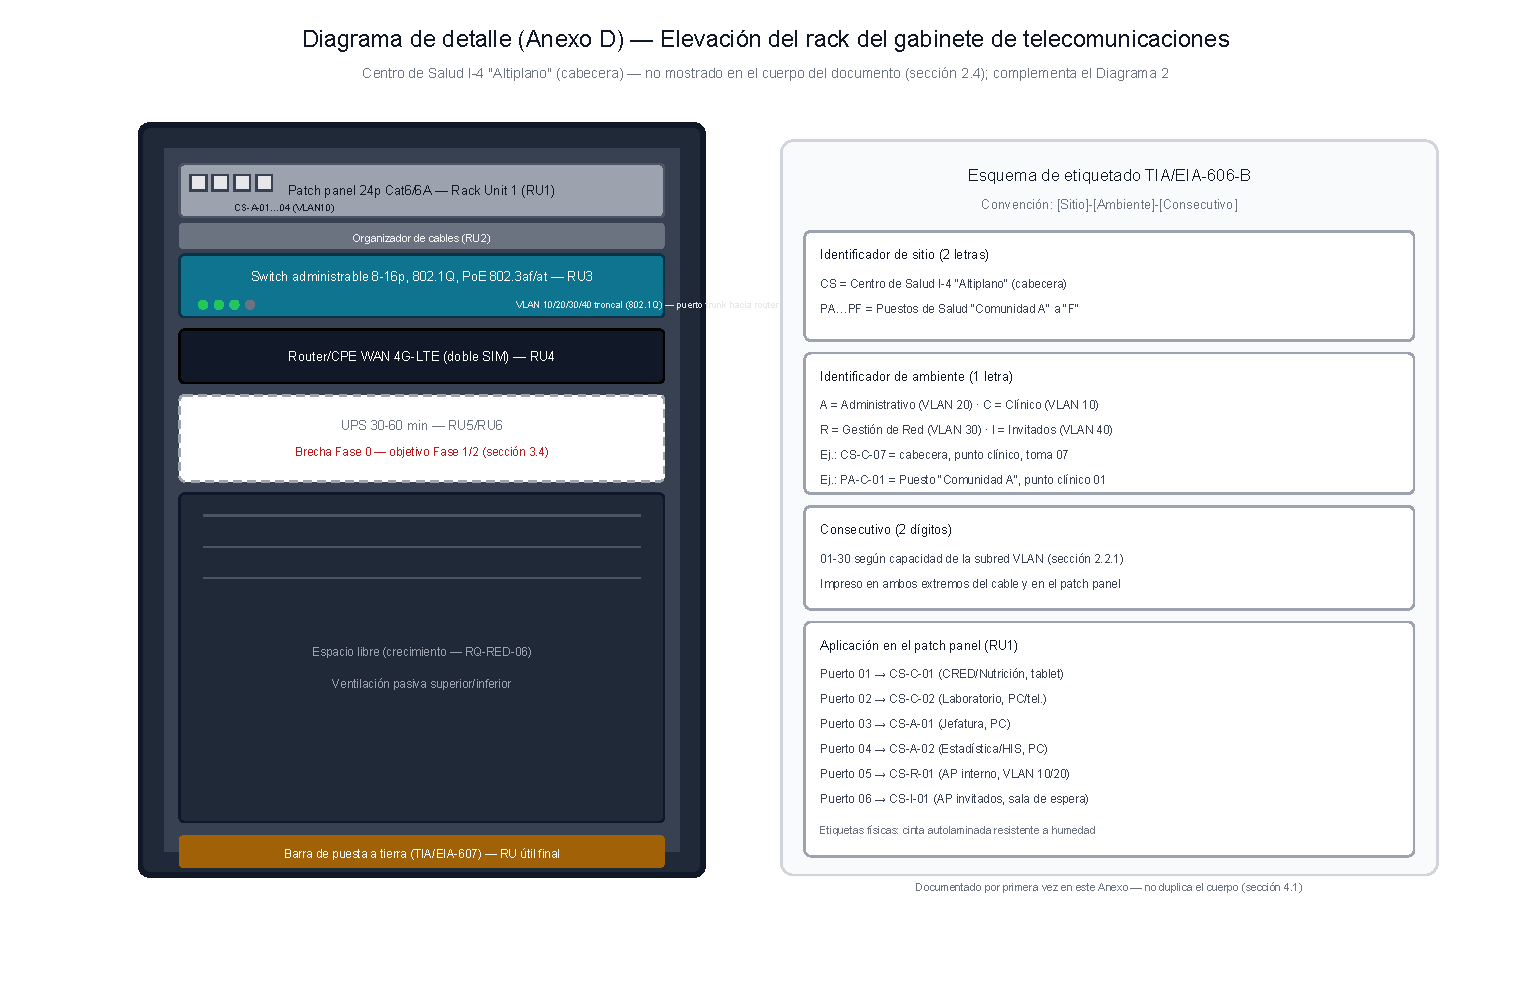
\includegraphics[width=0.88\linewidth,keepaspectratio]{assets/07-diseno-red/diagrama-anexo-d-rack-gabinete.pdf}}
\caption{Diagrama de detalle --- Elevación del rack del gabinete de telecomunicaciones}
\end{figure}

Este diagrama complementa el Diagrama 2 con un nivel de detalle que la vista de planta no puede mostrar: la elevación del rack (patch panel, switch, router/CPE, espacio reservado para UPS, barra de puesta a tierra) y el esquema de etiquetado TIA/EIA-606-B con la convención \textbf{{[}Sitio{]}-{[}Ambiente{]}-{[}Consecutivo{]}} (p.~ej., \texttt{CS-C-01} = cabecera, punto clínico 01; \texttt{PA-C-01} = Puesto ``Comunidad A'', punto clínico 01), aplicado de forma concreta a los primeros seis puertos del patch panel de la cabecera. Es, en sí mismo, el diagrama detallado exigido por la plantilla del entregable que no formaba parte del cuerpo del documento.

\subsection{Anexo E --- Estimación referencial de equipamiento de red de bajo costo (Fase 0, no oficial)}\label{anexo-e-estimaciuxf3n-referencial-de-equipamiento-de-red-de-bajo-costo-fase-0-no-oficial}

La siguiente tabla es una \textbf{estimación de ingeniería elaborada por el Integrante 1} a partir de precios de mercado peruano de orden de magnitud para equipos de red de bajo costo, sujeta a cotización real antes de cualquier adquisición. \textbf{No forma parte del presupuesto oficial y validado de S/ 3,124} (Entregables N.° 2 y N.° 3); se presenta como insumo de negociación con la microred anfitriona o de una eventual ampliación presupuestal.

{\small
\begin{longtable}[]{@{}
  >{\raggedright\arraybackslash}p{(\linewidth - 8\tabcolsep) * \real{0.2000}}
  >{\raggedright\arraybackslash}p{(\linewidth - 8\tabcolsep) * \real{0.2000}}
  >{\raggedright\arraybackslash}p{(\linewidth - 8\tabcolsep) * \real{0.2000}}
  >{\raggedright\arraybackslash}p{(\linewidth - 8\tabcolsep) * \real{0.2000}}
  >{\raggedright\arraybackslash}p{(\linewidth - 8\tabcolsep) * \real{0.2000}}@{}}
\toprule\noalign{}
\begin{minipage}[b]{\linewidth}\raggedright
Ítem
\end{minipage} & \begin{minipage}[b]{\linewidth}\raggedright
Cantidad
\end{minipage} & \begin{minipage}[b]{\linewidth}\raggedright
Costo unitario referencial (S/)
\end{minipage} & \begin{minipage}[b]{\linewidth}\raggedright
Subtotal referencial (S/)
\end{minipage} & \begin{minipage}[b]{\linewidth}\raggedright
Fase de adopción
\end{minipage} \\
\midrule\noalign{}
\endhead
\bottomrule\noalign{}
\endlastfoot
Router/CPE 4G-LTE con doble SIM (failover) & 1 & 450 & 450 & \textbf{Fase 0} --- adoptado como equipo WAN de la cabecera (sección 3.4); brecha de financiamiento de \textasciitilde=S/ 166 pendiente frente a la contingencia de S/ 284 \\
Switch administrable 8-16 puertos (802.1Q, PoE) & 1 & 400 & 400 & Sin fuente de financiamiento identificada \\
Puntos de acceso WiFi de doble banda & 2 & 200 & 400 & Sin fuente de financiamiento identificada \\
UPS de pequeña capacidad (protección de corte breve) & 1 & 280 & 280 & Objetivo Fase 1/2 (brecha declarada, sección 3.4) \\
Cableado, canaletas, conectores y patch panel pequeño & 1 (lote) & 200 & 200 & Sin fuente de financiamiento identificada \\
\textbf{TOTAL referencial (solo cabecera, Fase 0)} & & & \textbf{\textasciitilde= 1,730} & \\
\end{longtable}
}

\emph{Estimación referencial de ingeniería --- no validada, no oficial, sujeta a cotización real. No incluye los puestos de salud I-1/I-2, que en el diseño de la sección 2.5 no requieren equipamiento de segmentación dedicado, solo un CPE de bajo costo (obtenible como aporte de la microred anfitriona --- \textbf{{[}DATO PENDIENTE DE VALIDAR{]}}).} Para Fase 1/2, la sección 3.4 identifica que el salto de costo de hosting proyectado en el Business Case (\textasciitilde=S/ 1,200/año) ofrece una vía de financiamiento más natural para el resto del equipamiento que una ampliación puntual del presupuesto de Fase 0.

\subsection{Anexo F --- Verificación de consistencia con la arquitectura de software (Entregable N.° 5)}\label{anexo-f-verificaciuxf3n-de-consistencia-con-la-arquitectura-de-software-entregable-n.-5}

El paquete EDT 2.1 (Entregable N.° 3, sección 3.2.3) exige que este documento sea ``validado conjuntamente con Ingeniería de Software (paquete 4.3)''. Dicha validación conjunta formal ---una sesión de trabajo entre el Integrante 1 y el Integrante 3 con acta firmada--- \textbf{no se ha realizado todavía} y se declara como \textbf{{[}DATO PENDIENTE DE VALIDAR{]}}. A modo de verificación preliminar y de autocontrol, se presenta a continuación un cotejo de consistencia entre las decisiones de este documento y los artefactos ya fijados en el Entregable N.° 5, que deberá confirmarse o corregirse en la validación conjunta formal pendiente:

{\small
\begin{longtable}[]{@{}
  >{\raggedright\arraybackslash}p{(\linewidth - 4\tabcolsep) * \real{0.3333}}
  >{\raggedright\arraybackslash}p{(\linewidth - 4\tabcolsep) * \real{0.3333}}
  >{\raggedright\arraybackslash}p{(\linewidth - 4\tabcolsep) * \real{0.3333}}@{}}
\toprule\noalign{}
\begin{minipage}[b]{\linewidth}\raggedright
Artefacto del Entregable N.° 5
\end{minipage} & \begin{minipage}[b]{\linewidth}\raggedright
Decisión de este documento
\end{minipage} & \begin{minipage}[b]{\linewidth}\raggedright
¿Consistente?
\end{minipage} \\
\midrule\noalign{}
\endhead
\bottomrule\noalign{}
\endlastfoot
RF-01/RF-02 --- emparejamiento BLE \textless{} 10 s, captura sincronizada de 3 señales & Sección 2.7.1 diseña el enlace BLE como punto a punto, sin intermediarios de red, con recomendación de minimizar interferencia 2.4 GHz & Sí \\
ADR-01 --- offline-first con patrón \emph{outbox} & Secciones 2.7.4, 3.1 y 3.2 diseñan la red para no introducir dependencias de conectividad continua en el flujo clínico & Sí \\
ADR-02 --- monolito modular, backend único & Sección 2.2.2 aloja el backend en una única VPC con subred pública/privada, sin asumir microservicios distribuidos & Sí \\
ADR-08 --- aprendizaje federado presente pero inactivo en Fase 0 & Sección 2.2.2 reserva un bloque de direccionamiento (10.30.0.128/25) sin activarlo & Sí \\
ADR-09 --- Keycloak como identidad centralizada & Sección 2.3 protege el acceso a Keycloak mediante segmentación VLAN 20/30; sección 2.2.2 lo aloja en la subred privada, no expuesta directamente & Sí \\
ADR-10 --- PostgreSQL/PostGIS como único motor de base de datos & Sección 2.2.2 lo aloja junto al backend en la subred privada de la VPC & Sí \\
RNF-20 --- SLA del servidor pendiente de validar & Sección 3.1 no asume ningún SLA contratado y trata la redundancia de servidor como riesgo residual aceptado en Fase 0 & Sí, de forma consistente con la misma incertidumbre ya declarada en el Entregable N.° 5 \\
\end{longtable}
}

No se identifican, en este cotejo preliminar, contradicciones entre este documento y la arquitectura de software ya fijada. Se recomienda que la validación conjunta formal pendiente confirme, en particular, dos puntos que dependen de información que solo el paquete 4.3 (Firmware del nodo) puede precisar: la tasa de muestreo real de la ventana de captura BLE (sección 1.2.2) y la capacidad real del firmware para \emph{LE Secure Connections} (sección 2.7.1).

\begin{center}\rule{0.5\linewidth}{0.5pt}\end{center}

\section{Autoevaluación frente a la rúbrica}\label{autoevaluaciuxf3n-frente-a-la-ruxfabrica}

{\small
\begin{longtable}[]{@{}
  >{\raggedright\arraybackslash}p{(\linewidth - 4\tabcolsep) * \real{0.3333}}
  >{\raggedright\arraybackslash}p{(\linewidth - 4\tabcolsep) * \real{0.3333}}
  >{\raggedright\arraybackslash}p{(\linewidth - 4\tabcolsep) * \real{0.3333}}@{}}
\toprule\noalign{}
\begin{minipage}[b]{\linewidth}\raggedright
Criterio
\end{minipage} & \begin{minipage}[b]{\linewidth}\raggedright
Nivel alcanzado
\end{minipage} & \begin{minipage}[b]{\linewidth}\raggedright
Justificación
\end{minipage} \\
\midrule\noalign{}
\endhead
\bottomrule\noalign{}
\endlastfoot
Cumplimiento de la Plantilla del Producto (portada, extensión, Resumen Ejecutivo) & Bueno, con elementos de Excelente & El Resumen Ejecutivo se condensó a \textasciitilde=480 palabras (\textasciitilde=1 página) y el cuerpo se redujo de \textasciitilde=15,810 a \textasciitilde=13,400 palabras (-15 \%), fusionando los antiguos Anexos C y F (redundantes con el cuerpo) en un único Anexo C condensado y sintetizando los párrafos de justificación más largos de cada sección. Esta reducción \textbf{no basta por sí sola} para garantizar el rango de 15-20 páginas: dado el volumen de tablas técnicas que la propia rúbrica califica como Excelente (segmentación VLAN, SPOF, cumplimiento normativo) y que no deberían recortarse sin perder sustancia, una estimación conservadora sitúa el documento ya editado en \textasciitilde=24-30 páginas en formato Word estándar (interlineado 1.15-1.5, tablas y los tres diagramas vectoriales incluidos) --- una mejora real frente a las \textasciitilde=35-45 páginas de la versión previa, pero aún por encima del límite exigido. Se declara esto como \textbf{limitación residual honesta}: comprimir aún más exigiría eliminar tablas de contenido técnico ya evaluado como Excelente, lo que el equipo considera un costo mayor al beneficio de cumplir estrictamente el límite; se recomienda, como paso no aplicado en esta revisión, externalizar los Anexos B, D y E a un documento complementario si la plantilla lo permite, dejando el cuerpo (secciones 1-4) dentro de 15-20 páginas por sí solo. La portada, además, \textbf{no cumple aún literalmente} el requisito de incluir nombres reales de integrantes, asesor(a) y curso: se mantiene como \textbf{{[}DATO PENDIENTE DE VALIDAR{]}} y se declara \textbf{riesgo de entrega}, no dato ficticio. \\
Levantamiento de Requerimientos & Bueno, con elementos de Excelente & Integra aspectos técnicos (perfil de usuarios/dispositivos, ancho de banda con orden de magnitud justificado, RNF traducidos a requisitos de red) y de negocio (OE1-OE5, presupuesto, escalabilidad), con 14 RQ-RED trazables (sección 1.2.4, resumidos sin duplicar en el Anexo C). No alcanza ``Excelente'' pleno: el perfil de usuarios y el tráfico son estimaciones sin site survey real. \\
Diseño de Topología Lógica y Física & Excelente & Los Diagramas 2 y 3 (planta física) se produjeron con herramienta vectorial y simbología estándar (rack, RJ45, AP, color por VLAN), corrigiendo la limitación ASCII previa; su versión textual queda solo como referencia en el Anexo D, que además suma un diagrama de detalle inédito (rack + etiquetado TIA/EIA-606-B). Los Diagramas 1, 4 y 5, de naturaleza lógica, se mantienen como esquemas de texto ---convención aceptada para vistas de protocolo/failover---. Numeración consecutiva 1 a 5, sin saltos. \\
Aplicación de Segmentación (VLAN, DMZ, Subnetting) & Excelente & Esquema VLSM verificado (/27, /28, /29 sin solapamiento) bajo un /16 replicable por fases; matriz de acceso inter-VLAN con ejemplos concretos; reinterpretación justificada del concepto de DMZ para backend en nube, incluyendo el caso en que la DMZ física sí aplicaría (diferida). La asimetría cabecera/puestos unipersonales evidencia criterio de ingeniería, no plantilla mecánica. \\
Incorporación de Redundancia y Alta Disponibilidad & Bueno, con elementos de Excelente & SPOF de siete componentes (WAN de cabecera y de puestos I-1/I-2 separados), con RPO/RTO y un \emph{runbook} de cinco escenarios. A diferencia de la versión anterior, Fase 0 incorpora una \textbf{medida de redundancia física real}: router WAN dual-SIM en la cabecera (Anexo E, \textasciitilde=S/ 450). No alcanza ``Excelente'' pleno: esa medida tiene una brecha de financiamiento de \textasciitilde=S/ 166 sin cerrar (3.4), y el resto de las capas (servidor, switch/AP, WAN de los puestos, UPS) sigue sin redundancia real. \\
Cumplimiento de Estándares Internacionales & Excelente & Aplica TIA/EIA-568/569/606/607, ISO/IEC 11801 e IEEE 802.3/802.3af/802.11/802.1Q/802.1X/802.1D-w/802.15 a elementos concretos del diseño, con la precisión de que BLE es hoy gobernado por el Bluetooth SIG y no el IEEE, y 802.1X declarado como brecha de Fase 0. El etiquetado TIA/EIA-606-B, antes solo mencionado, ahora tiene un ejemplo concreto en el Anexo D. Suma cumplimiento sectorial (Ley 29733, DS 115-2025-PCM, OSIPTEL) con el hallazgo propio de NTP como requisito silencioso de auditabilidad. \\
Calidad Documental y Ética & Excelente & Sigue la plantilla exigida, lenguaje profesional consistente con los Entregables N.° 1, 2, 3 y 5, cita el Código ACM (2018) con cuatro principios aplicados concretamente, y marca cada límite con \textbf{{[}DATO PENDIENTE DE VALIDAR{]}}. Esta revisión corrigió: (i) numeración de diagramas, antes con salto deliberado (1,2,3,5,6), ahora consecutiva (1-5); (ii) redundancia Anexo C/F, fusionada; (iii) vacío de portada, declarado como riesgo de entrega en vez de placeholder silencioso. \\
\end{longtable}
}

\textbf{Limitación transversal declarada:} el nivel ``Excelente'' pleno en Levantamiento de Requerimientos, Redundancia y Plantilla del Producto requiere un site survey real, cotización real de equipos, el cierre de la brecha de \textasciitilde=S/ 166 de la redundancia WAN adoptada (3.4), la validación conjunta formal con el paquete EDT 4.3, y los nombres reales de portada. Ninguno existe a la fecha, por lo que se marcan \textbf{{[}DATO PENDIENTE DE VALIDAR{]}} o \textbf{riesgo de entrega}, sustituidos donde es posible por el cotejo de consistencia del Anexo F.

\clearpage
\renewcommand{\currentEntregable}{Infraestructura E2 --- Seguridad}
{\Large\bfseries Entregable 2 de Infraestructura (CE0321) --- Planificaci\'on de Seguridad\par}
\addcontentsline{toc}{section}{Entregable 2 de Infraestructura (CE0321) --- Planificaci\'on de Seguridad}
\bigskip

\textbf{Entregable N.° 8 --- Planificación de Seguridad}
\emph{(Octavo entregable consecutivo del proyecto HemoScan Andino. Corresponde al Entregable N.° 2 de la competencia CE032 --- Área A: Infraestructura Tecnológica; utiliza una numeración de entregable propia y distinta de la de los Entregables N.° 1-4 del Área B --- Gestión de TI--- y N.° 5 del Área C --- Ingeniería de Software--- ya presentados, aunque continúa la secuencia documental global del proyecto)}

\textbf{Área de competencia:} Área A --- Infraestructura Tecnológica
\textbf{Competencia:} CE032 --- Gestión de la Seguridad de la Información
\textbf{Evidencia que cubre este documento:} CE0321 --- Planificación de Seguridad (identificación de activos críticos, análisis de riesgos según ISO 27005/NIST, políticas de seguridad y roles y responsabilidades)

\textbf{Organización diagnosticada (caso ilustrativo y representativo):} Microred de Salud Altiplano-Puno

\begin{center}\rule{0.5\linewidth}{0.5pt}\end{center}

\textbf{Integrantes del equipo:}

{\small
\begin{longtable}[]{@{}
  >{\raggedright\arraybackslash}p{(\linewidth - 4\tabcolsep) * \real{0.3333}}
  >{\raggedright\arraybackslash}p{(\linewidth - 4\tabcolsep) * \real{0.3333}}
  >{\raggedright\arraybackslash}p{(\linewidth - 4\tabcolsep) * \real{0.3333}}@{}}
\toprule\noalign{}
\begin{minipage}[b]{\linewidth}\raggedright
N.°
\end{minipage} & \begin{minipage}[b]{\linewidth}\raggedright
Integrante
\end{minipage} & \begin{minipage}[b]{\linewidth}\raggedright
Rol / Área de competencia
\end{minipage} \\
\midrule\noalign{}
\endhead
\bottomrule\noalign{}
\endlastfoot
1 & \textit{(Integrante 1, Líder de Infraestructura Tecnológica -- nombre por completar)} & CE03 --- Infraestructura Tecnológica (red, seguridad, centro de datos) --- \textbf{responsable principal de este entregable} \\
2 & \textit{(Integrante 2, Líder de Gestión de TI -- nombre por completar)} & CE01 --- Gestión de TI (diagnóstico, business case, plan de gestión, procesos) \\
3 & \textit{(Integrante 3, Líder de Ingeniería de Software -- nombre por completar)} & CE02 --- Ingeniería de Software (requerimientos, datos, sistema, calidad) \\
\end{longtable}
}

\textbf{Docente asesor(a) del curso:} \textit{(nombre del docente asesor por completar)}
\textbf{Curso / Sílabo:} \textit{(nombre del curso / s\'ilabo por completar)}
\textbf{Ciclo académico:} 2026-I (supuesto, a confirmar con la programación académica vigente)

\textbf{Lugar y fecha:} Juliaca, Puno, Perú --- 07 de julio de 2026

\begin{center}\rule{0.5\linewidth}{0.5pt}\end{center}

\begin{quote}
\textbf{Nota metodológica y alcance (léase antes de continuar).} Este documento se apoya directamente en los entregables precedentes del proyecto: del \textbf{Entregable N.° 1} (Diagnóstico Organizacional) toma la caracterización de la organización ilustrativa \textbf{``Microred de Salud Altiplano-Puno''}, su bajo nivel de madurez digital en gobierno de TI y ciberseguridad (nivel 1 de 5, sección 1.3.2) y el inventario de sistemas de información existentes; del \textbf{Entregable N.° 2} (Business Case) toma el modelo de negocio B2G de 3 fases, el presupuesto de validación de Fase 0 (S/ 3,124) y el riesgo estratégico R5 ya identificado (``brecha de seguridad o incumplimiento de la Ley N.° 29733''), que este documento desarrolla y opera-cionaliza en detalle; del \textbf{Entregable N.° 3} (Plan de Gestión) toma el paquete de trabajo 2.3 ``Seguridad, identidad y control de acceso'' (asignado al Integrante 1, con el entregable ``ambiente de autenticación operativo + checklist de seguridad'' como criterio de aceptación); y del \textbf{Entregable N.° 5} (Requerimientos y Diseño del Sistema) toma íntegramente la arquitectura ya diseñada (backend FastAPI/NestJS, PostgreSQL+PostGIS, Keycloak OIDC/RBAC --- ADR-09---, servidor único de Fase 0 --- ADR-02, ADR-10---), los seis recursos FHIR del proyecto, los ocho actores del sistema y los requerimientos no funcionales de seguridad ya especificados (RNF-05 a RNF-07, RNF-18, RNF-19; RF-39, RF-40; RN-02 a RN-11). Este Entregable N.° 2 de la competencia CE032 \textbf{no rediseña} esa arquitectura: la toma como dada y construye sobre ella la capa de gobierno, gestión de riesgos y políticas de seguridad de la información que la rúbrica CE0321 exige.

Se mantiene vigente la misma advertencia metodológica de los entregables anteriores: HemoScan Andino \textbf{no cuenta todavía con un convenio real} con ninguna microred o posta de salud, ni con un comité de ética constituido, ni con un servidor de producción desplegado. Por ello, este plan de seguridad tiene naturaleza de \textbf{planificación previa (pre-despliegue)}: define los controles, políticas y roles que deberán estar operativos \textbf{antes} de procesar el primer dato real de un menor de edad en la Fase 0 de validación, no la certificación de un sistema ya operando. Su alcance es además \textbf{dual}, y esto se declara explícitamente para evitar ambigüedad: cubre (a) los activos propios de HemoScan Andino como organización emprendedora (código fuente, modelo de inteligencia artificial, dataset propietario, credenciales del equipo fundador) y (b) los activos que existirán en el entorno operativo de la organización cliente ilustrativa ``Microred de Salud Altiplano-Puno'' una vez desplegado el sistema (servidor de la posta, dispositivos de campo, cuentas del personal de salud), dado que el modelo de negocio B2G implica que la futura HemoScan Andino S.A.C. actuará como \textbf{encargada de tratamiento} de datos de salud sobre una infraestructura cuya modalidad exacta de alojamiento (servidor propio del equipo, nube comercial, o servidor físico dentro de la posta) es todavía \textbf{{[}DATO PENDIENTE DE VALIDAR: modalidad de alojamiento definitiva, a acordar contractualmente con la DIRESA/microred en la Fase 1{]}}. Todo valor numérico o afirmación normativa específica que no pueda derivarse razonablemente de lo ya declarado en el proyecto o de un estándar internacional de referencia pública (ISO/IEC 27001, ISO/IEC 27005, NIST) se marca explícitamente como \textbf{{[}DATO PENDIENTE DE VALIDAR{]}}, en lugar de presentarse como un hecho verificado.
\end{quote}

\begin{center}\rule{0.5\linewidth}{0.5pt}\end{center}

\section{Resumen Ejecutivo}\label{resumen-ejecutivo}

HemoScan Andino procesa, por definición de su propio modelo de negocio, uno de los tipos de datos más sensibles que contempla el ordenamiento jurídico peruano: datos de salud de menores de edad, agravados por la dimensión geográfica (comunidades altoandinas dispersas), la dimensión tecnológica (inteligencia artificial embebida clasificada como de alto riesgo por el Decreto Supremo N.° 115-2025-PCM) y la dimensión organizacional (una microred cuyo nivel de madurez en gobierno de TI y ciberseguridad fue diagnosticado, en el Entregable N.° 1, en el nivel más bajo de una escala de cinco). Este documento desarrolla la \textbf{Planificación de Seguridad} exigida por la competencia CE032 --- Gestión de la Seguridad de la Información, adoptando como marco metodológico central la familia de normas \textbf{ISO/IEC 27001:2022} (requisitos de un sistema de gestión de seguridad de la información), \textbf{ISO/IEC 27002:2022} (catálogo de controles) e \textbf{ISO/IEC 27005:2022} (gestión de riesgos de seguridad de la información), complementada con el proceso de evaluación de riesgos de \textbf{NIST SP 800-30 Rev.~1} y las seis funciones del \textbf{NIST Cybersecurity Framework (CSF) 2.0} (Gobernar, Identificar, Proteger, Detectar, Responder, Recuperar), en estricta observancia del DS 115-2025-PCM y de la Ley N.° 29733 de Protección de Datos Personales.

La \textbf{Sección 1} identifica y clasifica veintiocho activos críticos organizados en siete categorías (datos e información, credenciales y secretos, software, hardware, servicios, personas e intangibles), evaluados según el triángulo de confidencialidad, integridad y disponibilidad (CID), con propietario y custodio explícitos para cada uno. Se confirma que los activos de mayor criticidad global son, en este orden, los datos clínicos identificables de menores de edad, el servidor único que aloja el backend y la base de datos (punto único de falla ya reconocido en el Entregable N.° 5), y las credenciales/secretos de integración del backend.

La \textbf{Sección 2} aplica la metodología ISO 27005/NIST mediante una matriz semicuantitativa de diecinueve riesgos de seguridad de la información (identificados con el prefijo RS-01 a RS-19), cada uno con su amenaza, vulnerabilidad explotable, probabilidad e impacto en escala 1-5, puntaje de riesgo (probabilidad × impacto, rango 1-25) y nivel cualitativo resultante (Bajo, Moderado, Alto, Crítico). Cuatro riesgos alcanzan nivel Crítico: el acceso no autorizado por credenciales no revocadas ante la alta rotación del personal (régimen SERUMS), la pérdida o robo de un nodo/smartphone de campo con datos sin cifrar, la exposición accidental de secretos de configuración en un repositorio de código, y la ingeniería social dirigida al personal de salud. Estos resultados \textbf{desarrollan y operacionalizan}, con un método formal, el riesgo estratégico R5 ya declarado de forma cualitativa en el Business Case (Entregable N.° 2).

La \textbf{Sección 3} define once políticas de seguridad detalladas y aplicables ---control de accesos, protección de datos de menores, gestión criptográfica, dispositivos de campo y movilidad, copias de seguridad y continuidad, gestión de incidentes, desarrollo seguro, uso aceptable y concientización, gobernanza de inteligencia artificial, gestión de terceros, y un cierre de ética profesional alineado al Código de Ética y Conducta Profesional de la ACM---, cada una con lineamientos numerados, parámetros técnicos concretos (por ejemplo, cifrado TLS 1.2 o superior y AES-256 en reposo, autenticación multifactor para roles clínicos y administrativos, respaldo diario con prueba trimestral de restauración) y su control equivalente del Anexo A de ISO/IEC 27001:2022.

La \textbf{Sección 4} propone una estructura de gobierno de seguridad proporcional al tamaño real del equipo (tres integrantes en Fase 0), con una matriz RACI de doce procesos de seguridad que distingue las responsabilidades internas del equipo HemoScan Andino de las responsabilidades que, en un despliegue real, recaerán sobre el administrador del sistema de la microred y sobre el Comité de Ética/DIRESA como titular del banco de datos de salud, y plantea como hoja de ruta la creación de un rol formal de Oficial de Seguridad de la Información y de un Oficial de Protección de Datos una vez constituida HemoScan Andino S.A.C.

El cuerpo evaluable de este documento (Secciones 1 a 4, más los Anexos A, B y D) se ajusta al rango de 10-15 páginas indicado por la plantilla del entregable, y cierra con la matriz de riesgos completa con tratamiento y riesgo residual estimado (\textbf{Anexo A}), las referencias normativas y de estándares (\textbf{Anexo B}) y el checklist de seguridad que opera el criterio de aceptación del paquete EDT 2.3 del Plan de Gestión (\textbf{Anexo D}), este último ampliado con la verificación de la validación legal pendiente de las Políticas 3.2 y 3.6 (Sección 3.12). El glosario de términos y el índice de diagramas ---material útil pero no exigido por la plantilla--- se reclasifican como \textbf{material complementario de referencia}, ubicado después del cierre formal del cuerpo evaluable. Al final del documento se incluye, también fuera del cuerpo evaluable, una \textbf{nota interna de cobertura frente a la rúbrica} (no una autocalificación, tarea que corresponde exclusivamente al docente/evaluador) que documenta honestamente, como limitaciones centrales aún abiertas, la ausencia de una evaluación de riesgos validada con datos reales de incidentes, un pentest técnico ejecutado, un comité de ética constituido, y la validación legal peruana específica de los parámetros pendientes de las Políticas 3.2 y 3.6, insumos que solo estarán disponibles una vez formalizado un convenio institucional real.

\begin{center}\rule{0.5\linewidth}{0.5pt}\end{center}

\section{1. Identificación de Activos Críticos}\label{identificaciuxf3n-de-activos-cruxedticos}

\subsection{1.1 Metodología de identificación y clasificación}\label{metodologuxeda-de-identificaciuxf3n-y-clasificaciuxf3n}

La identificación de activos sigue el enfoque de \textbf{ISO/IEC 27001:2022, control A.5.9 (Inventario de información y otros activos asociados)}: todo activo que soporte el proceso de tamizaje de anemia infantil ---ya sea información, software, hardware, un servicio contratado o una persona con acceso privilegiado--- se registra con un identificador único (AC-01 a AC-28), su categoría, un \textbf{propietario} (quien decide su uso y clasificación) y un \textbf{custodio} (quien lo opera y protege técnicamente en el día a día), siguiendo la separación de responsabilidades que exige la norma.

Cada activo se valora según el triángulo clásico de seguridad de la información ---\textbf{Confidencialidad (C), Integridad (I) y Disponibilidad (D)}--- en una escala ordinal de tres niveles (Alta / Media / Baja), y se deriva una \textbf{criticidad global} igual al valor máximo alcanzado entre C, I y D, ajustada cualitativamente cuando el activo involucra datos de menores de edad o constituye un punto único de falla ya reconocido en la arquitectura (Entregable N.° 5, ADR-02 y ADR-10), en cuyo caso la criticidad global se fija en Alta con independencia del promedio matemático. Esta regla de ajuste es una decisión metodológica propia del equipo, no una prescripción literal de la norma, y se declara explícitamente por transparencia.

{\small
\begin{longtable}[]{@{}
  >{\raggedright\arraybackslash}p{(\linewidth - 6\tabcolsep) * \real{0.2500}}
  >{\raggedright\arraybackslash}p{(\linewidth - 6\tabcolsep) * \real{0.2500}}
  >{\raggedright\arraybackslash}p{(\linewidth - 6\tabcolsep) * \real{0.2500}}
  >{\raggedright\arraybackslash}p{(\linewidth - 6\tabcolsep) * \real{0.2500}}@{}}
\toprule\noalign{}
\begin{minipage}[b]{\linewidth}\raggedright
Nivel
\end{minipage} & \begin{minipage}[b]{\linewidth}\raggedright
Confidencialidad (C)
\end{minipage} & \begin{minipage}[b]{\linewidth}\raggedright
Integridad (I)
\end{minipage} & \begin{minipage}[b]{\linewidth}\raggedright
Disponibilidad (D)
\end{minipage} \\
\midrule\noalign{}
\endhead
\bottomrule\noalign{}
\endlastfoot
\textbf{Alta} & La divulgación no autorizada vulnera datos de salud de un menor de edad, secretos criptográficos o propiedad intelectual central del producto & La alteración no autorizada puede inducir un diagnóstico o tratamiento erróneo, o falsificar un registro de auditoría & La indisponibilidad detiene el tamizaje en campo o dejar sin operar el único servidor de la posta \\
\textbf{Media} & La divulgación afecta información operativa u organizacional sin exponer datos clínicos individuales de un menor & La alteración degrada la calidad del servicio o de un reporte, sin efecto clínico directo & La indisponibilidad es tolerable por horas gracias al diseño offline-first (RNF-03) \\
\textbf{Baja} & La divulgación tiene impacto marginal o es información ya pública/agregada & La alteración es detectable y corregible sin efecto sobre terceros & La indisponibilidad no afecta la operación crítica del tamizaje \\
\end{longtable}
}

\subsection{1.2 Inventario de activos críticos}\label{inventario-de-activos-cruxedticos}

\textbf{Datos e información}

{\small
\begin{longtable}[]{@{}
  >{\raggedright\arraybackslash}p{(\linewidth - 14\tabcolsep) * \real{0.1250}}
  >{\raggedright\arraybackslash}p{(\linewidth - 14\tabcolsep) * \real{0.1250}}
  >{\raggedright\arraybackslash}p{(\linewidth - 14\tabcolsep) * \real{0.1250}}
  >{\raggedright\arraybackslash}p{(\linewidth - 14\tabcolsep) * \real{0.1250}}
  >{\raggedright\arraybackslash}p{(\linewidth - 14\tabcolsep) * \real{0.1250}}
  >{\raggedright\arraybackslash}p{(\linewidth - 14\tabcolsep) * \real{0.1250}}
  >{\raggedright\arraybackslash}p{(\linewidth - 14\tabcolsep) * \real{0.1250}}
  >{\raggedright\arraybackslash}p{(\linewidth - 14\tabcolsep) * \real{0.1250}}@{}}
\toprule\noalign{}
\begin{minipage}[b]{\linewidth}\raggedright
ID
\end{minipage} & \begin{minipage}[b]{\linewidth}\raggedright
Activo
\end{minipage} & \begin{minipage}[b]{\linewidth}\raggedright
Propietario
\end{minipage} & \begin{minipage}[b]{\linewidth}\raggedright
Custodio
\end{minipage} & \begin{minipage}[b]{\linewidth}\raggedright
C
\end{minipage} & \begin{minipage}[b]{\linewidth}\raggedright
I
\end{minipage} & \begin{minipage}[b]{\linewidth}\raggedright
D
\end{minipage} & \begin{minipage}[b]{\linewidth}\raggedright
Criticidad global
\end{minipage} \\
\midrule\noalign{}
\endhead
\bottomrule\noalign{}
\endlastfoot
AC-01 & Datos clínicos identificables de menores de edad (recursos FHIR \emph{Patient} y \emph{Observation}) & Titular del banco de datos de salud (microred/DIRESA, futuro contrato) & Backend de interoperabilidad (Integrante 3) & Alta & Alta & Media & \textbf{Alta} \\
AC-02 & Consentimientos informados digitales (recurso FHIR \emph{Consent}) & Cuidador/a (titular del derecho) & Backend / App móvil & Alta & Alta & Media & \textbf{Alta} \\
AC-03 & Trazas de auditoría y procedencia (recursos FHIR \emph{Provenance}, \emph{AuditEvent}) & HemoScan Andino (equipo) & Servicio de Auditoría (backend) & Media & \textbf{Alta} & Media & \textbf{Alta} \\
AC-04 & Dataset propietario de entrenamiento (imágenes de conjuntiva, espectros AS7341, señales PPG MAX30102 y etiquetas de referencia HemoCue/ferritina/PCR) & HemoScan Andino (equipo) & Integrante 3 / repositorio de datos de entrenamiento & Alta & Alta & Media & \textbf{Alta} \\
AC-05 & Modelo de inferencia de IA entrenado (pesos ONNX/TFLite y su versionado) & HemoScan Andino (equipo) & Integrante 3 & Media & Alta & Media & \textbf{Alta} \\
AC-06 & Tabla/parámetros de corrección de hemoglobina por altitud y umbrales clínicos versionados (RN-02) & HemoScan Andino (equipo), validado por Personal médico & Backend (Configuración Clínica) & Media & \textbf{Alta} & Media & \textbf{Alta} \\
AC-07 & Motor de reglas de consejería nutricional (alineado a NTS 213-MINSA/DGIESP-2024) & HemoScan Andino (equipo) & Integrante 3 & Baja & Alta & Media & Media \\
AC-08 & Copias de respaldo (\emph{backups}) de la base de datos clínica y geoespacial & HemoScan Andino (equipo) & Integrante 1 & Alta & Alta & Alta & \textbf{Alta} \\
\end{longtable}
}

\textbf{Credenciales y secretos}

{\small
\begin{longtable}[]{@{}
  >{\raggedright\arraybackslash}p{(\linewidth - 14\tabcolsep) * \real{0.1250}}
  >{\raggedright\arraybackslash}p{(\linewidth - 14\tabcolsep) * \real{0.1250}}
  >{\raggedright\arraybackslash}p{(\linewidth - 14\tabcolsep) * \real{0.1250}}
  >{\raggedright\arraybackslash}p{(\linewidth - 14\tabcolsep) * \real{0.1250}}
  >{\raggedright\arraybackslash}p{(\linewidth - 14\tabcolsep) * \real{0.1250}}
  >{\raggedright\arraybackslash}p{(\linewidth - 14\tabcolsep) * \real{0.1250}}
  >{\raggedright\arraybackslash}p{(\linewidth - 14\tabcolsep) * \real{0.1250}}
  >{\raggedright\arraybackslash}p{(\linewidth - 14\tabcolsep) * \real{0.1250}}@{}}
\toprule\noalign{}
\begin{minipage}[b]{\linewidth}\raggedright
ID
\end{minipage} & \begin{minipage}[b]{\linewidth}\raggedright
Activo
\end{minipage} & \begin{minipage}[b]{\linewidth}\raggedright
Propietario
\end{minipage} & \begin{minipage}[b]{\linewidth}\raggedright
Custodio
\end{minipage} & \begin{minipage}[b]{\linewidth}\raggedright
C
\end{minipage} & \begin{minipage}[b]{\linewidth}\raggedright
I
\end{minipage} & \begin{minipage}[b]{\linewidth}\raggedright
D
\end{minipage} & \begin{minipage}[b]{\linewidth}\raggedright
Criticidad global
\end{minipage} \\
\midrule\noalign{}
\endhead
\bottomrule\noalign{}
\endlastfoot
AC-09 & Credenciales/secretos del backend (claves de base de datos, \emph{client secrets} de Keycloak, tokens de integración HIS-MINSA/Padrón Nominal/SIGA) & HemoScan Andino (equipo) & Integrante 1 & \textbf{Alta} & Alta & Media & \textbf{Alta} \\
AC-10 & Certificados TLS/SSL del backend FHIR y de la plataforma web & HemoScan Andino (equipo) & Integrante 1 & Media & Alta & Alta & \textbf{Alta} \\
AC-11 & Credenciales de acceso del personal de salud y agentes comunitarios (cuentas Keycloak, roles CRED/médico/farmacia) & Microred (futuro), HemoScan Andino (Fase 0) & Administrador del sistema & \textbf{Alta} & Media & Media & \textbf{Alta} \\
AC-12 & Credenciales administrativas (superusuario Keycloak, acceso raíz al servidor) & HemoScan Andino (equipo) & Integrante 1 & \textbf{Alta} & \textbf{Alta} & Media & \textbf{Alta} \\
\end{longtable}
}

\textbf{Software}

{\small
\begin{longtable}[]{@{}
  >{\raggedright\arraybackslash}p{(\linewidth - 14\tabcolsep) * \real{0.1250}}
  >{\raggedright\arraybackslash}p{(\linewidth - 14\tabcolsep) * \real{0.1250}}
  >{\raggedright\arraybackslash}p{(\linewidth - 14\tabcolsep) * \real{0.1250}}
  >{\raggedright\arraybackslash}p{(\linewidth - 14\tabcolsep) * \real{0.1250}}
  >{\raggedright\arraybackslash}p{(\linewidth - 14\tabcolsep) * \real{0.1250}}
  >{\raggedright\arraybackslash}p{(\linewidth - 14\tabcolsep) * \real{0.1250}}
  >{\raggedright\arraybackslash}p{(\linewidth - 14\tabcolsep) * \real{0.1250}}
  >{\raggedright\arraybackslash}p{(\linewidth - 14\tabcolsep) * \real{0.1250}}@{}}
\toprule\noalign{}
\begin{minipage}[b]{\linewidth}\raggedright
ID
\end{minipage} & \begin{minipage}[b]{\linewidth}\raggedright
Activo
\end{minipage} & \begin{minipage}[b]{\linewidth}\raggedright
Propietario
\end{minipage} & \begin{minipage}[b]{\linewidth}\raggedright
Custodio
\end{minipage} & \begin{minipage}[b]{\linewidth}\raggedright
C
\end{minipage} & \begin{minipage}[b]{\linewidth}\raggedright
I
\end{minipage} & \begin{minipage}[b]{\linewidth}\raggedright
D
\end{minipage} & \begin{minipage}[b]{\linewidth}\raggedright
Criticidad global
\end{minipage} \\
\midrule\noalign{}
\endhead
\bottomrule\noalign{}
\endlastfoot
AC-13 & Código fuente de la app móvil (Flutter/PWA) & HemoScan Andino (equipo) & Integrante 3 & Media & Alta & Media & Alta \\
AC-14 & Código fuente del backend de interoperabilidad (FastAPI/NestJS) & HemoScan Andino (equipo) & Integrante 3 & Media & Alta & Media & Alta \\
AC-15 & Firmware del nodo (C/C++, ESP32-S3) & HemoScan Andino (equipo) & Integrante 1 & Baja & Alta & Media & Media \\
AC-16 & Sistema de identidad Keycloak (configuración de \emph{realm}, políticas OIDC/RBAC --- ADR-09) & HemoScan Andino (equipo) & Integrante 1 & Media & \textbf{Alta} & Alta & \textbf{Alta} \\
AC-17 & Plataforma web de analítica geoespacial (React/TypeScript) & HemoScan Andino (equipo) & Integrante 3 & Baja & Media & Media & Media \\
\end{longtable}
}

\textbf{Hardware}

{\small
\begin{longtable}[]{@{}
  >{\raggedright\arraybackslash}p{(\linewidth - 14\tabcolsep) * \real{0.1250}}
  >{\raggedright\arraybackslash}p{(\linewidth - 14\tabcolsep) * \real{0.1250}}
  >{\raggedright\arraybackslash}p{(\linewidth - 14\tabcolsep) * \real{0.1250}}
  >{\raggedright\arraybackslash}p{(\linewidth - 14\tabcolsep) * \real{0.1250}}
  >{\raggedright\arraybackslash}p{(\linewidth - 14\tabcolsep) * \real{0.1250}}
  >{\raggedright\arraybackslash}p{(\linewidth - 14\tabcolsep) * \real{0.1250}}
  >{\raggedright\arraybackslash}p{(\linewidth - 14\tabcolsep) * \real{0.1250}}
  >{\raggedright\arraybackslash}p{(\linewidth - 14\tabcolsep) * \real{0.1250}}@{}}
\toprule\noalign{}
\begin{minipage}[b]{\linewidth}\raggedright
ID
\end{minipage} & \begin{minipage}[b]{\linewidth}\raggedright
Activo
\end{minipage} & \begin{minipage}[b]{\linewidth}\raggedright
Propietario
\end{minipage} & \begin{minipage}[b]{\linewidth}\raggedright
Custodio
\end{minipage} & \begin{minipage}[b]{\linewidth}\raggedright
C
\end{minipage} & \begin{minipage}[b]{\linewidth}\raggedright
I
\end{minipage} & \begin{minipage}[b]{\linewidth}\raggedright
D
\end{minipage} & \begin{minipage}[b]{\linewidth}\raggedright
Criticidad global
\end{minipage} \\
\midrule\noalign{}
\endhead
\bottomrule\noalign{}
\endlastfoot
AC-18 & Nodos de hardware HemoScan Andino en campo (ESP32-S3 + AS7341 + MAX30102 + LED) & HemoScan Andino (equipo) & Integrante 1 / Personal CRED en uso & Media & Media & Alta & Alta \\
AC-19 & Smartphones del personal de campo (Personal CRED/médico) & Microred (futuro) / personal (Fase 0) & Personal CRED / Personal médico & \textbf{Alta} & Media & Alta & \textbf{Alta} \\
AC-20 & Servidor/nube único de la posta (backend + BD + Keycloak --- ADR-02, ADR-10) & HemoScan Andino (equipo) & Integrante 1 & Alta & Alta & \textbf{Alta} & \textbf{Alta} \\
AC-21 & Equipo de referencia HemoCue usado en la validación clínica de Fase 0 & Microred ilustrativa (préstamo/convenio) & Personal médico / Personal CRED & Baja & Alta & Media & Media \\
\end{longtable}
}

\textbf{Servicios}

{\small
\begin{longtable}[]{@{}
  >{\raggedright\arraybackslash}p{(\linewidth - 14\tabcolsep) * \real{0.1250}}
  >{\raggedright\arraybackslash}p{(\linewidth - 14\tabcolsep) * \real{0.1250}}
  >{\raggedright\arraybackslash}p{(\linewidth - 14\tabcolsep) * \real{0.1250}}
  >{\raggedright\arraybackslash}p{(\linewidth - 14\tabcolsep) * \real{0.1250}}
  >{\raggedright\arraybackslash}p{(\linewidth - 14\tabcolsep) * \real{0.1250}}
  >{\raggedright\arraybackslash}p{(\linewidth - 14\tabcolsep) * \real{0.1250}}
  >{\raggedright\arraybackslash}p{(\linewidth - 14\tabcolsep) * \real{0.1250}}
  >{\raggedright\arraybackslash}p{(\linewidth - 14\tabcolsep) * \real{0.1250}}@{}}
\toprule\noalign{}
\begin{minipage}[b]{\linewidth}\raggedright
ID
\end{minipage} & \begin{minipage}[b]{\linewidth}\raggedright
Activo
\end{minipage} & \begin{minipage}[b]{\linewidth}\raggedright
Propietario
\end{minipage} & \begin{minipage}[b]{\linewidth}\raggedright
Custodio
\end{minipage} & \begin{minipage}[b]{\linewidth}\raggedright
C
\end{minipage} & \begin{minipage}[b]{\linewidth}\raggedright
I
\end{minipage} & \begin{minipage}[b]{\linewidth}\raggedright
D
\end{minipage} & \begin{minipage}[b]{\linewidth}\raggedright
Criticidad global
\end{minipage} \\
\midrule\noalign{}
\endhead
\bottomrule\noalign{}
\endlastfoot
AC-22 & Integración con sistemas externos (HIS-MINSA, Padrón Nominal, SIGA) & MINSA / MEF-RENIEC (dato externo) & Integrante 3 (conector) & Alta & Alta & Media & Alta \\
AC-23 & Servicio de hosting/nube contratado & HemoScan Andino (equipo) & Integrante 1 & Media & Media & \textbf{Alta} & Alta \\
AC-24 & Servicio de notificaciones push/SMS a cuidadores & HemoScan Andino (equipo) & Integrante 3 & Media & Baja & Media & Media \\
\end{longtable}
}

\textbf{Personas}

{\small
\begin{longtable}[]{@{}
  >{\raggedright\arraybackslash}p{(\linewidth - 14\tabcolsep) * \real{0.1250}}
  >{\raggedright\arraybackslash}p{(\linewidth - 14\tabcolsep) * \real{0.1250}}
  >{\raggedright\arraybackslash}p{(\linewidth - 14\tabcolsep) * \real{0.1250}}
  >{\raggedright\arraybackslash}p{(\linewidth - 14\tabcolsep) * \real{0.1250}}
  >{\raggedright\arraybackslash}p{(\linewidth - 14\tabcolsep) * \real{0.1250}}
  >{\raggedright\arraybackslash}p{(\linewidth - 14\tabcolsep) * \real{0.1250}}
  >{\raggedright\arraybackslash}p{(\linewidth - 14\tabcolsep) * \real{0.1250}}
  >{\raggedright\arraybackslash}p{(\linewidth - 14\tabcolsep) * \real{0.1250}}@{}}
\toprule\noalign{}
\begin{minipage}[b]{\linewidth}\raggedright
ID
\end{minipage} & \begin{minipage}[b]{\linewidth}\raggedright
Activo
\end{minipage} & \begin{minipage}[b]{\linewidth}\raggedright
Propietario
\end{minipage} & \begin{minipage}[b]{\linewidth}\raggedright
Custodio
\end{minipage} & \begin{minipage}[b]{\linewidth}\raggedright
C
\end{minipage} & \begin{minipage}[b]{\linewidth}\raggedright
I
\end{minipage} & \begin{minipage}[b]{\linewidth}\raggedright
D
\end{minipage} & \begin{minipage}[b]{\linewidth}\raggedright
Criticidad global
\end{minipage} \\
\midrule\noalign{}
\endhead
\bottomrule\noalign{}
\endlastfoot
AC-25 & Personal de salud (CRED, médico, farmacia) como custodio operativo de datos y dispositivos & Microred (futuro) & Jefatura de microred & Alta & Media & Alta & Alta \\
AC-26 & Equipo HemoScan Andino (los 3 integrantes) como custodio de código, infraestructura y llaves & HemoScan Andino (equipo) & Los 3 integrantes & \textbf{Alta} & \textbf{Alta} & \textbf{Alta} & \textbf{Alta} \\
\end{longtable}
}

\textbf{Intangibles}

{\small
\begin{longtable}[]{@{}
  >{\raggedright\arraybackslash}p{(\linewidth - 14\tabcolsep) * \real{0.1250}}
  >{\raggedright\arraybackslash}p{(\linewidth - 14\tabcolsep) * \real{0.1250}}
  >{\raggedright\arraybackslash}p{(\linewidth - 14\tabcolsep) * \real{0.1250}}
  >{\raggedright\arraybackslash}p{(\linewidth - 14\tabcolsep) * \real{0.1250}}
  >{\raggedright\arraybackslash}p{(\linewidth - 14\tabcolsep) * \real{0.1250}}
  >{\raggedright\arraybackslash}p{(\linewidth - 14\tabcolsep) * \real{0.1250}}
  >{\raggedright\arraybackslash}p{(\linewidth - 14\tabcolsep) * \real{0.1250}}
  >{\raggedright\arraybackslash}p{(\linewidth - 14\tabcolsep) * \real{0.1250}}@{}}
\toprule\noalign{}
\begin{minipage}[b]{\linewidth}\raggedright
ID
\end{minipage} & \begin{minipage}[b]{\linewidth}\raggedright
Activo
\end{minipage} & \begin{minipage}[b]{\linewidth}\raggedright
Propietario
\end{minipage} & \begin{minipage}[b]{\linewidth}\raggedright
Custodio
\end{minipage} & \begin{minipage}[b]{\linewidth}\raggedright
C
\end{minipage} & \begin{minipage}[b]{\linewidth}\raggedright
I
\end{minipage} & \begin{minipage}[b]{\linewidth}\raggedright
D
\end{minipage} & \begin{minipage}[b]{\linewidth}\raggedright
Criticidad global
\end{minipage} \\
\midrule\noalign{}
\endhead
\bottomrule\noalign{}
\endlastfoot
AC-27 & Reputación institucional y confianza pública (``licencia social para operar'') & HemoScan Andino (equipo) & Equipo / futura S.A.C. & Media & \textbf{Alta} & Baja & Alta \\
AC-28 & Propiedad intelectual del algoritmo de fusión multisensor y de autocalibración por altitud (potencial modelo de utilidad/patente, ya anotado como riesgo competitivo R10 en el Business Case) & HemoScan Andino (equipo) & Integrante 3 & Alta & Media & Baja & Alta \\
\end{longtable}
}

\subsection{1.3 Síntesis de activos de máxima criticidad}\label{suxedntesis-de-activos-de-muxe1xima-criticidad}

Del inventario de veintiocho activos, veintitrés (el 82 \%) alcanzan criticidad global \textbf{Alta}, cinco se clasifican como Media y ninguno como Baja, lo que confirma cuantitativamente la observación cualitativa ya hecha en el Entregable N.° 1: una organización con datos de máxima sensibilidad (salud de menores) y una arquitectura deliberadamente concentrada en un único servidor de bajo costo (ADR-02, ADR-10) no tiene margen para tratar la seguridad de la información como un asunto secundario. Cinco activos merecen mención explícita como prioridad absoluta de protección, por concentrar simultáneamente alta confidencialidad, alta integridad y relevancia legal directa: \textbf{AC-01} (datos clínicos de menores), \textbf{AC-02} (consentimientos, precondición legal obligatoria de cualquier captura por RN-04), \textbf{AC-09} y \textbf{AC-12} (credenciales/secretos, cuya exposición compromete transitivamente a todos los demás activos del backend) y \textbf{AC-20} (el servidor único, cuya pérdida de disponibilidad detiene la operación completa del backend, Keycloak y la base de datos a la vez). Esta síntesis es la que orienta la priorización de riesgos de la Sección 2 y el diseño de controles de la Sección 3. Como mejora no obligatoria para esta etapa de planificación pre-despliegue, se recomienda ---una vez desplegado el servidor de producción--- contrastar este inventario documental contra un \textbf{CMDB (\emph{Configuration Management Database}) técnico real}, verificando que cada activo aquí declarado corresponda exactamente a un elemento de configuración operativo y detectando activos no documentados que puedan haberse incorporado durante la implementación.

\begin{center}\rule{0.5\linewidth}{0.5pt}\end{center}

\section{2. Análisis de Riesgos (ISO 27005 / NIST)}\label{anuxe1lisis-de-riesgos-iso-27005-nist}

\subsection{2.1 Metodología}\label{metodologuxeda}

El análisis de riesgos adopta el proceso de \textbf{ISO/IEC 27005:2022} ---establecimiento del contexto, identificación del riesgo, análisis del riesgo (probabilidad × consecuencia), evaluación del riesgo frente a criterios de aceptación, y tratamiento del riesgo---, complementado con el modelo de \textbf{NIST SP 800-30 Rev.~1}, que descompone cada escenario en una \textbf{fuente de amenaza} (humana deliberada, humana accidental, ambiental o de falla técnica), un \textbf{evento de amenaza} que explota una \textbf{vulnerabilidad} concreta del activo, produciendo un \textbf{impacto adverso}. La siguiente tabla resume la correspondencia entre ambos marcos y las seis funciones del NIST CSF 2.0, usada como verificación cruzada de cobertura:

{\small
\begin{longtable}[]{@{}
  >{\raggedright\arraybackslash}p{(\linewidth - 4\tabcolsep) * \real{0.3333}}
  >{\raggedright\arraybackslash}p{(\linewidth - 4\tabcolsep) * \real{0.3333}}
  >{\raggedright\arraybackslash}p{(\linewidth - 4\tabcolsep) * \real{0.3333}}@{}}
\toprule\noalign{}
\begin{minipage}[b]{\linewidth}\raggedright
Fase ISO/IEC 27005:2022
\end{minipage} & \begin{minipage}[b]{\linewidth}\raggedright
Paso equivalente NIST SP 800-30
\end{minipage} & \begin{minipage}[b]{\linewidth}\raggedright
Función NIST CSF 2.0 relacionada
\end{minipage} \\
\midrule\noalign{}
\endhead
\bottomrule\noalign{}
\endlastfoot
Establecimiento del contexto & Preparación de la evaluación & Gobernar (\emph{Govern}) \\
Identificación del riesgo & Identificación de fuentes y eventos de amenaza, y de vulnerabilidades & Identificar (\emph{Identify}) \\
Análisis y evaluación del riesgo & Determinación de probabilidad e impacto; cálculo del riesgo & Identificar (\emph{Identify}) / Proteger (\emph{Protect}) \\
Tratamiento del riesgo & Comunicación de resultados y priorización de controles & Proteger (\emph{Protect}), Detectar (\emph{Detect}) \\
Monitoreo y revisión & Mantenimiento de la evaluación & Detectar (\emph{Detect}), Responder (\emph{Respond}), Recuperar (\emph{Recover}) \\
\end{longtable}
}

Para el cálculo, se emplea una escala semicuantitativa de \textbf{1 a 5} tanto para probabilidad como para impacto, con un puntaje de riesgo igual a \textbf{probabilidad × impacto} (rango 1-25), clasificado en cuatro bandas:

{\small
\begin{longtable}[]{@{}
  >{\raggedright\arraybackslash}p{(\linewidth - 4\tabcolsep) * \real{0.3333}}
  >{\raggedright\arraybackslash}p{(\linewidth - 4\tabcolsep) * \real{0.3333}}
  >{\raggedright\arraybackslash}p{(\linewidth - 4\tabcolsep) * \real{0.3333}}@{}}
\toprule\noalign{}
\begin{minipage}[b]{\linewidth}\raggedright
Puntaje (P × I)
\end{minipage} & \begin{minipage}[b]{\linewidth}\raggedright
Nivel de riesgo
\end{minipage} & \begin{minipage}[b]{\linewidth}\raggedright
Criterio de tratamiento
\end{minipage} \\
\midrule\noalign{}
\endhead
\bottomrule\noalign{}
\endlastfoot
16 - 25 & \textbf{Crítico} & Tratamiento inmediato; requiere control compensatorio antes de procesar el primer dato real de un menor \\
11 - 15 & \textbf{Alto} & Tratamiento prioritario dentro del paquete EDT 2.3 (Fase 0) \\
6 - 10 & \textbf{Moderado} & Tratamiento planificado dentro del roadmap de Fase 1 \\
1 - 5 & \textbf{Bajo} & Aceptar y monitorear; revisar en cada ciclo de revisión del SGSI (sección 4) \\
\end{longtable}
}

\textbf{Escala de probabilidad:} (1) Muy baja --- improbable en el horizonte de Fase 0-1; (2) Baja --- podría ocurrir de forma excepcional; (3) Media --- es razonable que ocurra en algún momento del piloto; (4) Alta --- se considera probable dado el contexto ya diagnosticado (madurez digital nivel 1, rotación SERUMS, dispersión geográfica); (5) Muy alta --- existen indicios concretos de que ya ocurre de forma análoga (por ejemplo, el uso ya diagnosticado de \emph{shadow IT}).

\textbf{Escala de impacto:} (1) Insignificante; (2) Menor --- molestia operativa sin efecto clínico ni legal; (3) Moderado --- degradación del servicio sin exposición de datos de menores; (4) Mayor --- exposición parcial de datos o indisponibilidad prolongada; (5) Catastrófico --- compromiso de datos clínicos de menores de edad, decisión clínica errónea inducida, o incumplimiento grave de la Ley N.° 29733 o del DS 115-2025-PCM.

\subsection{2.2 Taxonomía de fuentes de amenaza consideradas}\label{taxonomuxeda-de-fuentes-de-amenaza-consideradas}

Siguiendo la taxonomía de NIST SP 800-30, se consideran cuatro fuentes de amenaza aplicables al contexto de HemoScan Andino: \textbf{(a) humana deliberada} (atacante externo, personal interno malicioso, suplantación de identidad); \textbf{(b) humana accidental} (error de configuración, extravío de un dispositivo, publicación accidental de un secreto, uso de canales informales por desconocimiento); \textbf{(c) ambiental/estructural} (condiciones de campo altoandinas ya diagnosticadas en el Entregable N.° 1: dispersión geográfica, conectividad y electricidad intermitentes, clima extremo); y \textbf{(d) falla técnica} (indisponibilidad del servidor único, expiración no gestionada de certificados, defectos de software). Cada riesgo de la matriz siguiente se etiqueta con su fuente de amenaza predominante.

\subsection{2.3 Matriz de riesgos de seguridad de la información (riesgo inherente)}\label{matriz-de-riesgos-de-seguridad-de-la-informaciuxf3n-riesgo-inherente}

La matriz siguiente desarrolla, con método formal, el riesgo estratégico \textbf{R5} ya identificado cualitativamente en el Business Case (Entregable N.° 2: ``brecha de seguridad o incumplimiento de la Ley N.° 29733\ldots{} Probabilidad Baja, Impacto Crítico, Nivel Alto'') y lo descompone en diecinueve escenarios técnicos específicos y auditables.

{\small
\begin{longtable}[]{@{}
  >{\raggedright\arraybackslash}p{(\linewidth - 16\tabcolsep) * \real{0.1111}}
  >{\raggedright\arraybackslash}p{(\linewidth - 16\tabcolsep) * \real{0.1111}}
  >{\raggedright\arraybackslash}p{(\linewidth - 16\tabcolsep) * \real{0.1111}}
  >{\raggedright\arraybackslash}p{(\linewidth - 16\tabcolsep) * \real{0.1111}}
  >{\raggedright\arraybackslash}p{(\linewidth - 16\tabcolsep) * \real{0.1111}}
  >{\raggedright\arraybackslash}p{(\linewidth - 16\tabcolsep) * \real{0.1111}}
  >{\raggedright\arraybackslash}p{(\linewidth - 16\tabcolsep) * \real{0.1111}}
  >{\raggedright\arraybackslash}p{(\linewidth - 16\tabcolsep) * \real{0.1111}}
  >{\raggedright\arraybackslash}p{(\linewidth - 16\tabcolsep) * \real{0.1111}}@{}}
\toprule\noalign{}
\begin{minipage}[b]{\linewidth}\raggedright
ID
\end{minipage} & \begin{minipage}[b]{\linewidth}\raggedright
Activo(s) (AC-\#\#)
\end{minipage} & \begin{minipage}[b]{\linewidth}\raggedright
Fuente
\end{minipage} & \begin{minipage}[b]{\linewidth}\raggedright
Amenaza
\end{minipage} & \begin{minipage}[b]{\linewidth}\raggedright
Vulnerabilidad explotada
\end{minipage} & \begin{minipage}[b]{\linewidth}\raggedright
P
\end{minipage} & \begin{minipage}[b]{\linewidth}\raggedright
I
\end{minipage} & \begin{minipage}[b]{\linewidth}\raggedright
Riesgo
\end{minipage} & \begin{minipage}[b]{\linewidth}\raggedright
Nivel
\end{minipage} \\
\midrule\noalign{}
\endhead
\bottomrule\noalign{}
\endlastfoot
RS-01 & AC-01, AC-11 & Humana accidental & Acceso indebido a historiales clínicos de menores mediante cuentas de personal saliente no desactivadas a tiempo & Ausencia de proceso formal de baja inmediata de cuentas Keycloak al finalizar el periodo SERUMS (alta rotación, Entregable N.° 1) & 4 & 5 & 20 & \textbf{Crítico} \\
RS-02 & AC-01, AC-08, AC-20 & Humana deliberada & Exfiltración o filtración masiva de la base de datos clínica por explotación de una vulnerabilidad del backend expuesto a internet & Backend sin \emph{hardening}, gestión de parches ni \emph{firewall} de aplicaciones web (WAF); cifrado en reposo aún no verificado en la práctica & 3 & 5 & 15 & Alto \\
RS-03 & AC-20 & Falla técnica & Indisponibilidad total del sistema por sobrecarga o ataque de denegación de servicio al servidor único (backend + BD + Keycloak, ADR-02/ADR-10) & Arquitectura de un único servidor sin redundancia ni balanceo de carga & 3 & 4 & 12 & Alto \\
RS-04 & AC-08, AC-20 & Falla técnica & Pérdida irreversible de datos clínicos e históricos por ausencia o falla de copias de seguridad periódicas & No existe todavía una política formal de respaldo ni prueba documentada de restauración & 3 & 5 & 15 & Alto \\
RS-05 & AC-18, AC-19 & Ambiental / humana accidental & Pérdida, robo o extravío de un nodo o \emph{smartphone} de campo con datos clínicos en el búfer \emph{offline} local & Dispersión geográfica (Entregable N.° 1, 1.1.1) y ausencia de cifrado de almacenamiento local o de borrado/bloqueo remoto & 4 & 4 & 16 & \textbf{Crítico} \\
RS-06 & AC-09, AC-14 & Humana accidental & Exposición de credenciales/secretos (claves de BD, \emph{client secret} de Keycloak, tokens HIS-MINSA) por publicación accidental en un repositorio de código & Falta de gestión de secretos (variables de entorno/\emph{vault}) y de revisión previa a cada \emph{commit}/\emph{push}, riesgo típico de repositorios académicos & 4 & 4 & 16 & \textbf{Crítico} \\
RS-07 & AC-06 & Humana deliberada & Alteración no autorizada de la tabla de corrección de hemoglobina por altitud o de los umbrales clínicos & Ausencia de control de integridad (firma/hash) y de doble aprobación sobre cambios en la configuración clínica parametrizable (RN-02) & 2 & 5 & 10 & Moderado \\
RS-08 & AC-01, AC-16 & Humana deliberada & Suplantación del rol ``Personal médico'' para ejecutar confirmaciones diagnósticas o prescripciones sin autorización real (\emph{bypass} de RN-06) & Ausencia de autenticación multifactor para roles clínicos críticos & 2 & 5 & 10 & Moderado \\
RS-09 & AC-10 & Falla técnica & Interceptación o degradación de la confidencialidad en tránsito por certificado TLS expirado o mal configurado & Proceso de renovación de certificados no automatizado (costo ya presupuestado en el Entregable N.° 2, sin procedimiento operativo definido) & 3 & 4 & 12 & Alto \\
RS-10 & AC-01 & Humana deliberada / accidental & Reidentificación indirecta de niños o familias a partir de datos ``anonimizados'' del mapa de cobertura/riesgo si la celda H3 es demasiado fina en zonas de muy baja densidad & Falta de un umbral mínimo de agregación (\emph{k}-anonimato) antes de exponer una celda H3 en la plataforma web (brecha de implementación de RN-08) & 3 & 4 & 12 & Alto \\
RS-11 & AC-15, AC-18 & Humana deliberada & Manipulación del firmware del nodo mediante carga de firmware no autorizado & Ausencia de actualización OTA firmada criptográficamente y de verificación de integridad del firmware & 2 & 3 & 6 & Moderado \\
RS-12 & AC-18 & Humana deliberada & Interceptación (\emph{sniffing}) del canal BLE entre el nodo y la app durante la transmisión de señales ópticas crudas & Emparejamiento BLE sin cifrado GATT reforzado ni verificación de vínculo (\emph{bonding}) & 2 & 3 & 6 & Moderado \\
RS-13 & AC-25 & Humana deliberada & Ingeniería social/\emph{phishing} dirigido al personal de salud o al administrador del sistema para obtener credenciales & Baja madurez de ciberseguridad y concientización del personal (Entregable N.° 1, nivel 1/5 en gobierno de TI y ciberseguridad) & 4 & 4 & 16 & \textbf{Crítico} \\
RS-14 & AC-01 & Humana accidental & Uso de canales no oficiales (mensajería instantánea informal, \emph{shadow IT}) para compartir información clínica entre personal de salud & Práctica ya diagnosticada en el Entregable N.° 1 (sección 1.3.1) como canal sin trazabilidad institucional & 4 & 3 & 12 & Alto \\
RS-15 & AC-04, AC-05 & Humana deliberada & Manipulación del dataset o de las actualizaciones del modelo durante el reentrenamiento federado (\emph{data/model poisoning}), una vez activado en Fase 1/2 (ADR-08) & Ausencia de validación de integridad de las actualizaciones de parámetros recibidas de cada posta & 2 & 4 & 8 & Moderado \\
RS-16 & AC-26 & Estructural / organizacional & Concentración del conocimiento técnico y de accesos privilegiados en un solo integrante (``\emph{bus factor}''), sin respaldo documentado de configuraciones críticas & Equipo de 3 personas sin documentación de continuidad ni acceso de respaldo (relacionado con el riesgo organizacional R9 del Business Case) & 3 & 3 & 9 & Moderado \\
RS-17 & AC-05, AC-28 & Humana accidental & Registro auditable incompleto de recomendaciones generadas por el componente de IA, dificultando demostrar cumplimiento del DS 115-2025-PCM & Implementación parcial o tardía de RF-40 (registro de toda recomendación de IA con supervisión humana explícita) & 3 & 4 & 12 & Alto \\
RS-18 & AC-21, AC-22 & Humana accidental & Ruptura de la cadena de custodia de datos durante la validación cruzada con HemoCue/ferritina-PCR de Fase 0 & Coexistencia temporal de registro digital (HemoScan) y registro manual del laboratorio de referencia durante la validación & 3 & 3 & 9 & Moderado \\
RS-19 & AC-18 & Cadena de suministro & Sustitución o adulteración de componentes electrónicos (AS7341, MAX30102) por un proveedor no autorizado & Proceso de adquisición sin verificación de autenticidad ni proveedor único certificado (riesgo ya anotado como R6 en el Business Case) & 2 & 2 & 4 & Bajo \\
\end{longtable}
}

\subsection{2.4 Mapa de calor de riesgo inherente (probabilidad × impacto)}\label{mapa-de-calor-de-riesgo-inherente-probabilidad-impacto}

\begin{samepage}\begin{verbatim}
                          P=1          P=2                P=3                        P=4                     P=5
 I=5 Catastrófico          —      RS-07, RS-08       RS-02, RS-04                  RS-01                      —
 I=4 Mayor                 —         RS-15        RS-03,RS-09,RS-10,RS-17    RS-05,RS-06,RS-13                —
 I=3 Moderado              —      RS-11, RS-12       RS-16, RS-18                RS-14                       —
 I=2 Menor                 —         RS-19                —                        —                         —
 I=1 Insignificante        —           —                  —                        —                         —
\end{verbatim}\end{samepage}

\textbf{Leyenda de bandas:} celdas con puntaje 16-25 (esquina superior derecha) = Crítico; 11-15 = Alto; 6-10 = Moderado; 1-5 = Bajo (esquina inferior izquierda).

\subsection{2.5 Priorización y estrategia de tratamiento}\label{priorizaciuxf3n-y-estrategia-de-tratamiento}

De los diecinueve riesgos identificados, \textbf{cuatro son de nivel Crítico} (RS-01, RS-05, RS-06, RS-13), \textbf{siete de nivel Alto} (RS-02, RS-03, RS-04, RS-09, RS-10, RS-14, RS-17), \textbf{siete de nivel Moderado} (RS-07, RS-08, RS-11, RS-12, RS-15, RS-16, RS-18) y \textbf{uno de nivel Bajo} (RS-19). Es relevante notar que \textbf{ninguno de los cuatro riesgos críticos corresponde a un ataque técnicamente sofisticado}: los cuatro se originan en debilidades de gestión (falta de proceso de baja de cuentas, falta de cifrado de dispositivos de campo, falta de gestión de secretos, falta de concientización del personal), lo que confirma un hallazgo consistente con el diagnóstico digital del Entregable N.° 1 (nivel de madurez 1/5 en gobierno de TI y ciberseguridad): la prioridad de tratamiento de Fase 0 no es adquirir herramientas de seguridad sofisticadas, sino \textbf{cerrar brechas de proceso básicas} antes de tocar el primer dato real de un menor. En términos de las cuatro opciones de tratamiento de ISO/IEC 27005 (modificar/mitigar, retener/aceptar, evitar, compartir/transferir), este documento \textbf{mitiga} dieciséis de los diecinueve riesgos mediante controles técnicos y de proceso (Sección 3), \textbf{transfiere} parcialmente el riesgo de disponibilidad del hosting (RS-03) mediante la elección de un proveedor de nube con SLA propio en Fase 1 ---una vez resuelto el \textbf{{[}DATO PENDIENTE DE VALIDAR: SLA objetivo del servidor, ya señalado como pendiente en el Entregable N.° 5, RNF-20{]}}---, \textbf{evita} la activación prematura del riesgo de envenenamiento de modelo (RS-15) al mantener el aprendizaje federado inactivo hasta Fase 1/2 (decisión ya tomada en ADR-08) y \textbf{acepta con monitoreo} el único riesgo de nivel Bajo (RS-19), por su naturaleza de cadena de suministro externa al control directo del equipo. El desarrollo completo del tratamiento y del riesgo residual estimado para cada uno de los diecinueve riesgos se presenta en el \textbf{Anexo A}.

\begin{center}\rule{0.5\linewidth}{0.5pt}\end{center}

\section{3. Políticas de Seguridad}\label{poluxedticas-de-seguridad}

Las siguientes once políticas traducen el análisis de riesgos de la Sección 2 en reglas concretas, aplicables y auditables. Cada política indica su objetivo, sus lineamientos numerados, el o los controles equivalentes del \textbf{Anexo A de ISO/IEC 27001:2022} (citados de forma general por tema, dado el carácter público y estandarizado de dicho catálogo) y su vínculo con los requerimientos ya definidos en el Entregable N.° 5. Todas las políticas rigen desde la Fase 0 de validación, no solo desde un eventual despliegue comercial.

\subsection{3.1 Política de Control de Accesos}\label{poluxedtica-de-control-de-accesos}

\textbf{Objetivo:} garantizar que cada usuario acceda únicamente a la información y funciones estrictamente necesarias para su rol (principio de mínimo privilegio), en cumplimiento de RNF-06 y RF-37.

\begin{enumerate}
\def\labelenumi{\arabic{enumi}.}
\tightlist
\item
  Toda autenticación se realiza exclusivamente a través de Keycloak (OIDC); ninguna aplicación ni servicio de HemoScan Andino almacena contraseñas propias (ADR-09, ya decidido en el Entregable N.° 5).
\item
  Se definen, como mínimo, los cuatro roles funcionales exigidos por RNF-06 (Personal CRED, Personal médico, Administrador del sistema, Auditor), ampliables a los ocho actores humanos identificados en el Entregable N.° 5, cada uno con permisos explícitamente delimitados y probados antes de la ejecución de campo.
\item
  Se exige \textbf{autenticación multifactor (MFA)} obligatoria para los roles Administrador del sistema, Personal médico y Auditor/Comité de ética, dado que estos roles pueden confirmar diagnósticos, prescribir tratamiento o acceder a trazas de auditoría completas (mitiga RS-08). Para el rol Personal CRED, dado el uso de teléfonos de gama baja/media y la posible intermitencia de señal para MFA por SMS, se exige como mínimo una contraseña robusta (12 caracteres, complejidad) más vínculo de dispositivo (\emph{device binding}), evaluándose MFA por aplicación de autenticación (TOTP) offline como mejora incremental --- \textbf{{[}DATO PENDIENTE DE VALIDAR: factibilidad de TOTP offline en los modelos de smartphone finalmente adquiridos{]}}.
\item
  Toda cuenta de personal de salud debe darse de baja o suspenderse \textbf{el mismo día} en que finaliza su vínculo con la microred (incluyendo el término del periodo SERUMS), mediante un procedimiento formal de notificación de la Jefatura de microred al Administrador del sistema (mitiga directamente RS-01, el riesgo Crítico de mayor puntaje de toda la matriz).
\item
  Se realiza una \textbf{revisión trimestral} de cuentas activas y de sus roles asignados, documentada y firmada por el Administrador del sistema.
\item
  Toda cuenta se bloquea automáticamente tras 5 intentos fallidos de autenticación consecutivos, con un tiempo de bloqueo mínimo de 15 minutos.
\item
  Las acciones de ``confirmación diagnóstica'' y ``prescripción'' permanecen reservadas de forma exclusiva al rol Personal médico a nivel de backend (no solo de interfaz), conforme RN-06, de modo que ninguna manipulación del cliente móvil pueda otorgar privilegios no autorizados.
\end{enumerate}

\emph{Controles ISO/IEC 27001:2022 relacionados:} A.5.15 (Control de acceso), A.5.16 (Gestión de identidad), A.5.17 (Información de autenticación), A.5.18 (Derechos de acceso), A.8.2 (Derechos de acceso privilegiado), A.8.5 (Autenticación segura).

\subsection{3.2 Política de Protección de Datos Personales y de Salud de Menores de Edad}\label{poluxedtica-de-protecciuxf3n-de-datos-personales-y-de-salud-de-menores-de-edad}

\textbf{Objetivo:} cumplir la Ley N.° 29733 y sus principios (legalidad, consentimiento, finalidad, proporcionalidad, calidad, seguridad y disposición de recurso), reconociendo la sensibilidad máxima de tratar datos de salud de personas menores de edad.

\begin{enumerate}
\def\labelenumi{\arabic{enumi}.}
\tightlist
\item
  Ninguna captura de señales ópticas se inicia sin un recurso FHIR \emph{Consent} previamente registrado, vigente y verificable (RN-04); el firmante debe acreditar su relación de parentesco o tutela con el menor.
\item
  Se aplica el principio de \textbf{minimización de datos}: solo se recolectan los campos estrictamente necesarios para el tamizaje, la corrección por altitud y la trazabilidad exigida; no se solicitan datos adicionales ``por si acaso''.
\item
  Todo dato expuesto en la plataforma web de analítica geoespacial (mapa de cobertura/riesgo) debe agregarse a un nivel mínimo de \emph{k}-anonimato por hexágono H3 antes de su publicación, nunca a nivel de individuo identificable (RN-08); se fija como parámetro de partida un mínimo de \textbf{k \textgreater= 5} casos por celda expuesta, sujeto a validación estadística posterior --- \textbf{{[}DATO PENDIENTE DE VALIDAR: umbral óptimo de \emph{k} según la densidad poblacional real de la microred{]}}.
\item
  Se reconoce expresamente que, en un despliegue real, el \textbf{titular del banco de datos de salud} es la entidad de salud (microred/DIRESA), mientras que HemoScan Andino S.A.C. actúa como \textbf{encargada de tratamiento} bajo un acuerdo contractual que deberá especificar finalidad, plazo de conservación y prohibición de uso secundario no autorizado --- \textbf{{[}DATO PENDIENTE DE VALIDAR: cláusulas exactas del futuro contrato de encargo de tratamiento{]}}.
\item
  Los datos utilizados para analítica poblacional agregada (Sección 2.5 y RN-09 del Entregable N.° 5) se anonimizan de forma irreversible antes de cualquier uso secundario (planificación regional, publicaciones académicas).
\item
  Se reconoce a los cuidadores el ejercicio de los derechos de acceso, rectificación, cancelación y oposición (derechos ARCO) sobre los datos de sus hijos, mediante un procedimiento a definir con la Jefatura de microred --- \textbf{{[}DATO PENDIENTE DE VALIDAR: procedimiento operativo exacto y plazo de respuesta, a definir en coordinación con la Autoridad Nacional de Protección de Datos Personales{]}}.
\item
  El plazo de conservación de los datos clínicos se alinea al que exija la normativa de historias clínicas del sector salud peruano --- \textbf{{[}DATO PENDIENTE DE VALIDAR: plazo legal exacto de conservación{]}} ---; mientras tanto, se adopta como valor operativo provisional un mínimo de 15 años desde la última atención, revisable.
\item
  Toda solicitud de acceso a datos clínicos de un menor por un rol de auditoría, incluyendo accesos de solo lectura, se registra sin excepción en un recurso \emph{AuditEvent} (RN-11).
\end{enumerate}

\emph{Controles ISO/IEC 27001:2022 relacionados:} A.5.34 (Privacidad y protección de datos personales), A.5.12 (Clasificación de la información), A.5.33 (Protección de registros), A.8.10 (Eliminación de información).

\subsection{3.3 Política de Gestión Criptográfica}\label{poluxedtica-de-gestiuxf3n-criptogruxe1fica}

\textbf{Objetivo:} proteger la confidencialidad e integridad de los datos en tránsito y en reposo (RNF-05, RF-39), y eliminar la exposición de secretos identificada como riesgo Crítico (RS-06).

\begin{enumerate}
\def\labelenumi{\arabic{enumi}.}
\tightlist
\item
  Todo tráfico entre la app móvil, la plataforma web y el backend se cifra con \textbf{TLS 1.2 como mínimo}, con preferencia por TLS 1.3 cuando el hardware de referencia lo soporte.
\item
  Los datos en reposo en la base de datos PostgreSQL/PostGIS se cifran a nivel de disco/columna sensible con \textbf{AES-256} o algoritmo de fortaleza equivalente.
\item
  Ningún secreto (claves de base de datos, \emph{client secrets} de Keycloak, tokens de integración con HIS-MINSA/Padrón Nominal/SIGA) se almacena en texto plano dentro del código fuente ni se sube a un repositorio de control de versiones; se gestionan mediante variables de entorno o un gestor de secretos dedicado, con revisión automatizada previa a cada \emph{commit} (mitiga directamente RS-06).
\item
  Los certificados TLS se renuevan mediante un procedimiento automatizado (por ejemplo, renovación programada con al menos 30 días de anticipación al vencimiento), eliminando la dependencia de un recordatorio manual (mitiga RS-09); el costo de esta renovación ya fue presupuestado como partida de mantenimiento en el Entregable N.° 2.
\item
  Las llaves criptográficas y los certificados raíz se resguardan bajo custodia exclusiva del Integrante 1 (Infraestructura Tecnológica), con una copia de respaldo cifrada y accesible por un segundo integrante designado, para mitigar el riesgo de ``\emph{bus factor}'' (RS-16).
\item
  El firmware del nodo únicamente admite actualizaciones \emph{over-the-air} firmadas criptográficamente, rechazando cualquier imagen de firmware no verificada (mitiga RS-11).
\end{enumerate}

\emph{Controles ISO/IEC 27001:2022 relacionados:} A.8.24 (Uso de criptografía), A.8.9 (Gestión de la configuración), A.8.12 (Prevención de fuga de datos).

\subsection{3.4 Política de Seguridad de Dispositivos de Campo y Movilidad}\label{poluxedtica-de-seguridad-de-dispositivos-de-campo-y-movilidad}

\textbf{Objetivo:} proteger los nodos de hardware y los \emph{smartphones} de campo frente a pérdida, robo o manipulación, dado el contexto de dispersión geográfica ya diagnosticado (Entregable N.° 1) y el riesgo Crítico RS-05.

\begin{enumerate}
\def\labelenumi{\arabic{enumi}.}
\tightlist
\item
  Todo \emph{smartphone} de campo activa cifrado de almacenamiento a nivel de sistema operativo y bloqueo de pantalla obligatorio (PIN/biometría) antes de instalar la app HemoScan Andino.
\item
  El búfer de sincronización \emph{offline} (cola de \emph{outbox}, ADR-01) se cifra en el almacenamiento local del dispositivo, de modo que la pérdida física del equipo no exponga datos clínicos en texto plano.
\item
  Se mantiene un inventario físico actualizado de los nodos y \emph{smartphones} asignados por establecimiento, con responsable nombrado (vínculo directo con el inventario de activos AC-18/AC-19 de la Sección 1).
\item
  Ante la pérdida o robo reportado de un dispositivo, el Administrador del sistema revoca de inmediato las credenciales asociadas y, si la plataforma móvil lo permite, ejecuta borrado remoto del contenido de la app.
\item
  Los nodos de hardware no se dejan sin supervisión en zonas de acceso público durante las jornadas de campo; su transporte sigue el protocolo ya definido por el paquete EDT 2.5 (Soporte de infraestructura en campo) del Plan de Gestión.
\item
  Se prohíbe expresamente el uso de dispositivos personales no inventariados (BYOD no controlado) para capturar, almacenar o transmitir datos clínicos de pacientes.
\end{enumerate}

\emph{Controles ISO/IEC 27001:2022 relacionados:} A.7.9 (Seguridad de los activos fuera de las instalaciones), A.8.1 (Dispositivos \emph{endpoint} de usuario).

\subsection{3.5 Política de Copias de Seguridad y Continuidad Operativa}\label{poluxedtica-de-copias-de-seguridad-y-continuidad-operativa}

\textbf{Objetivo:} garantizar la disponibilidad y recuperabilidad de los datos clínicos ante la falla del servidor único (AC-20), mitigando el riesgo Alto RS-04.

\begin{enumerate}
\def\labelenumi{\arabic{enumi}.}
\tightlist
\item
  Se ejecuta una copia de seguridad \textbf{incremental diaria} y una copia \textbf{completa semanal} de la base de datos PostgreSQL/PostGIS y de la configuración de Keycloak.
\item
  Las copias se retienen en una ventana móvil de 90 días, más un respaldo mensual conservado durante 12 meses, almacenado en una ubicación lógicamente separada del servidor de producción.
\item
  Se ejecuta una \textbf{prueba de restauración trimestral} documentada, verificando que la copia es efectivamente utilizable y no solo generada.
\item
  Se define un objetivo de tiempo de recuperación (\textbf{RTO \textless= 24 horas}) y un objetivo de punto de recuperación (\textbf{RPO \textless= 24 horas}) como metas propuestas por este documento para la Fase 0, en ausencia de un SLA contractual definido (RNF-20 del Entregable N.° 5 ya señala esta cifra como pendiente de validar con el proveedor final).
\item
  Se documenta un plan mínimo de continuidad operativa que reconoce explícitamente la limitación arquitectónica de un único servidor (ADR-02/ADR-10): ante una falla mayor, el modo \emph{offline-first} del cliente móvil (RNF-03, hasta 72 horas de autonomía) actúa como mitigación temporal mientras se restaura el servicio, evitando la pérdida de capturas ya realizadas en campo.
\end{enumerate}

\emph{Controles ISO/IEC 27001:2022 relacionados:} A.8.13 (Copias de seguridad de la información), A.5.30 (Preparación de las TIC para la continuidad del negocio), A.5.29 (Seguridad de la información durante la disrupción).

\subsection{3.6 Política de Gestión de Incidentes de Seguridad}\label{poluxedtica-de-gestiuxf3n-de-incidentes-de-seguridad}

\textbf{Objetivo:} detectar, contener, comunicar y aprender de cualquier incidente de seguridad, con especial atención a brechas que involucren datos de menores de edad.

\begin{enumerate}
\def\labelenumi{\arabic{enumi}.}
\tightlist
\item
  Todo incidente se clasifica en cuatro niveles de severidad ---Crítico, Alto, Moderado, Bajo--- usando la misma escala de la Sección 2, y se registra en una bitácora de incidentes desde su detección.
\item
  Un incidente que exponga o pueda haber expuesto datos clínicos de un menor de edad se escala internamente al Integrante 2 (responsable de cumplimiento) en un plazo objetivo de \textbf{24 horas} desde su detección.
\item
  Se evalúa, dentro de un plazo objetivo interno de \textbf{72 horas} desde la detección, si el incidente amerita notificación a la Autoridad Nacional de Protección de Datos Personales y a los cuidadores afectados; se aclara expresamente que este plazo de 72 horas es un \textbf{objetivo interno de buena práctica propuesto por este documento}, inspirado en estándares internacionales comparables, y no una cifra confirmada como plazo legal peruano exigido --- \textbf{{[}DATO PENDIENTE DE VALIDAR: plazo legal exacto de notificación de brechas bajo la Ley N.° 29733 y su Reglamento{]}}.
\item
  Todo incidente cerrado genera una revisión de causa raíz y una actualización correspondiente de la matriz de riesgos de la Sección 2, cerrando el ciclo de mejora continua exigido por un sistema de gestión de seguridad de la información.
\item
  El uso de canales informales (mensajería instantánea personal) para reportar un incidente que involucre datos de pacientes queda expresamente prohibido, en coherencia con la Política 3.8.
\end{enumerate}

\emph{Controles ISO/IEC 27001:2022 relacionados:} A.5.24 (Planificación y preparación de la gestión de incidentes), A.5.25 (Evaluación y decisión sobre eventos de seguridad), A.5.26 (Respuesta a incidentes), A.5.27 (Aprendizaje de los incidentes), A.6.8 (Reporte de eventos de seguridad de la información).

\subsection{3.7 Política de Desarrollo Seguro (Secure SDLC)}\label{poluxedtica-de-desarrollo-seguro-secure-sdlc}

\textbf{Objetivo:} incorporar la seguridad desde el diseño (``\emph{security by design}'') en el ciclo de vida de desarrollo de la app móvil, el backend y el firmware.

\begin{enumerate}
\def\labelenumi{\arabic{enumi}.}
\tightlist
\item
  Todo cambio de código pasa por revisión de al menos un segundo integrante antes de integrarse a la rama principal (\emph{code review} obligatorio); el repositorio se configura además con protección de rama principal y con un mecanismo automatizado de detección de secretos expuestos (mitiga en parte el ``\emph{bus factor}'' RS-16 y refuerza estructuralmente la mitigación de RS-06).
\item
  Las dependencias de terceros (bibliotecas de Flutter, paquetes Python/Node del backend) se revisan periódicamente contra vulnerabilidades conocidas (CVE) antes de cada incremento de \emph{sprint}, y se mantienen ambientes separados de desarrollo, pruebas y producción, usando en desarrollo y pruebas exclusivamente datos sintéticos o anonimizados ---nunca datos clínicos reales---.
\item
  Ninguna funcionalidad que module reglas de negocio críticas (RN-01 a RN-12) se despliega a producción sin evidencia de prueba funcional y de seguridad, coherente con el paquete EDT 4.7 (Aseguramiento de la calidad) del Plan de Gestión.
\end{enumerate}

\emph{Controles ISO/IEC 27001:2022 relacionados:} A.8.25 (Ciclo de vida de desarrollo seguro), A.8.28 (Codificación segura), A.8.29 (Pruebas de seguridad en desarrollo y aceptación).

\subsection{3.8 Política de Uso Aceptable y Concientización en Seguridad}\label{poluxedtica-de-uso-aceptable-y-concientizaciuxf3n-en-seguridad}

\textbf{Objetivo:} elevar la madurez de ciberseguridad del personal de salud, hoy diagnosticada en el nivel más bajo de la escala (Entregable N.° 1, sección 1.3.2), y mitigar el riesgo Crítico RS-13 (ingeniería social).

\begin{enumerate}
\def\labelenumi{\arabic{enumi}.}
\tightlist
\item
  Todo integrante del equipo y todo miembro del personal de salud que use el sistema recibe una capacitación mínima de concientización en seguridad (reconocimiento de \emph{phishing}, gestión de contraseñas, manejo adecuado de dispositivos) antes de operar el sistema con datos reales, aprovechando la misma jornada de preparación logística y de campo ya prevista en el paquete EDT 3.6 del Plan de Gestión (Entregable N.° 3) y la partida presupuestal de ``materiales de gestión, consejería nutricional impresa y capacitación'' ya definida en el Business Case (Entregable N.° 2).
\item
  Se prohíbe expresamente el uso de mensajería instantánea personal no oficial (\emph{shadow IT}) para compartir cualquier dato identificable de un paciente, atacando directamente la práctica ya diagnosticada en el Entregable N.° 1 y el riesgo RS-14 de esta matriz.
\item
  Se prohíbe compartir credenciales de acceso entre distintos usuarios, incluso entre compañeros del mismo establecimiento en situaciones de aparente urgencia operativa.
\item
  Todo usuario debe reportar de inmediato cualquier sospecha de correo, mensaje o llamada de \emph{phishing} dirigidos a sus credenciales del sistema, sin sanción por el solo hecho de reportar (cultura de reporte no punitiva).
\item
  El lenguaje de toda comunicación de seguridad dirigida al personal de campo debe ser simple y no alarmista, en coherencia con RNF-14 ya definido en el Entregable N.° 5, y contemplar la pertinencia intercultural (quechua/aymara) cuando sea aplicable.
\end{enumerate}

\emph{Controles ISO/IEC 27001:2022 relacionados:} A.6.3 (Concientización, educación y capacitación en seguridad de la información), A.6.8 (Reporte de eventos de seguridad).

\subsection{3.9 Política de Gobernanza de Inteligencia Artificial y Trazabilidad}\label{poluxedtica-de-gobernanza-de-inteligencia-artificial-y-trazabilidad}

\textbf{Objetivo:} dar cumplimiento operativo al DS 115-2025-PCM, que clasifica a la salud como sector de alto riesgo para sistemas de IA y exige supervisión humana significativa y trazabilidad auditable.

\begin{enumerate}
\def\labelenumi{\arabic{enumi}.}
\tightlist
\item
  Ninguna recomendación, alerta o clasificación de severidad generada por el modelo de inferencia se ejecuta como decisión autónoma; toda confirmación diagnóstica y prescripción requiere una acción explícita de un profesional de salud humano autenticado (RN-01, RN-10, ya definidos en el Entregable N.° 5).
\item
  Toda inferencia del modelo, junto con su versión de modelo y de firmware, se registra de forma auditable (RF-40, RNF-18), cerrando la brecha identificada en el riesgo RS-17 de esta matriz.
\item
  Todo cambio en la tabla de corrección por altitud o en los umbrales clínicos se versiona y queda trazable a las determinaciones históricas a las que se aplicó cada versión (RN-02, CA-10 del Entregable N.° 5), con doble validación técnica (Integrante 3) y clínica (Personal médico referente).
\item
  El reentrenamiento federado (Flower), cuando se active en Fase 1/2 (ADR-08), transfiere exclusivamente actualizaciones de parámetros del modelo, nunca datos crudos de pacientes fuera del nodo/posta de origen (RN-09), y valida la integridad de cada actualización recibida antes de incorporarla (mitigación de RS-15).
\item
  Se mantiene una bitácora de gobernanza de IA disponible para consulta del rol Auditor/Comité de ética (CU-10 del Entregable N.° 5), documentando qué decisiones fueron asistidas por IA y cuál fue la acción humana de supervisión correspondiente.
\end{enumerate}

\emph{Controles ISO/IEC 27001:2022 relacionados:} A.5.31 (Requisitos legales, estatutarios, regulatorios y contractuales), A.8.16 (Actividades de monitoreo); referencia normativa directa: DS 115-2025-PCM.

\subsection{3.10 Política de Gestión de Terceros y Cadena de Suministro}\label{poluxedtica-de-gestiuxf3n-de-terceros-y-cadena-de-suministro}

\textbf{Objetivo:} extender el control de seguridad a los sistemas externos (HIS-MINSA, Padrón Nominal, SIGA) y a los proveedores de componentes de hardware.

\begin{enumerate}
\def\labelenumi{\arabic{enumi}.}
\tightlist
\item
  Toda integración con un sistema externo, así como cualquier tercero con acceso a datos clínicos o a infraestructura de HemoScan Andino (por ejemplo, un proveedor de hosting en Fase 1), se formaliza mediante un acuerdo o protocolo técnico que especifique el alcance exacto de los datos intercambiados ---minimizado a lo estrictamente necesario para la interoperabilidad FHIR--- y un compromiso de confidencialidad y cumplimiento mínimo equivalente a las políticas de este documento.
\item
  Los proveedores de componentes electrónicos (AS7341, MAX30102, ESP32-S3) se seleccionan preferentemente de canales oficiales o distribuidores autorizados, con verificación básica de autenticidad al recibir cada lote, para mitigar el riesgo Bajo RS-19 y el riesgo de cadena de suministro R6 ya anotado en el Business Case.
\end{enumerate}

\emph{Controles ISO/IEC 27001:2022 relacionados:} A.5.19, A.5.20, A.5.21, A.5.22 (Seguridad de la información en las relaciones con proveedores y en la cadena de suministro de TIC).

\subsection{3.11 Ética profesional (Código de Ética y Conducta Profesional de la ACM) y responsabilidad social}\label{uxe9tica-profesional-cuxf3digo-de-uxe9tica-y-conducta-profesional-de-la-acm-y-responsabilidad-social}

Esta planificación de seguridad no se concibe únicamente como un ejercicio de cumplimiento normativo, sino como una responsabilidad ética directa del equipo, en línea con el \textbf{Código de Ética y Conducta Profesional de la ACM (2018)}. En particular, el principio \textbf{1.2 (Evitar el daño)} exige anticipar que un fallo de seguridad en este sistema no es un incidente abstracto de TI, sino uno que puede afectar directamente a un niño o niña y a la confianza de su familia en el sistema de salud; el principio \textbf{1.6 (Respetar la privacidad)} y \textbf{1.7 (Honrar la confidencialidad)} sustentan directamente la Política 3.2; el principio \textbf{2.5 (Ofrecer evaluaciones exhaustivas de los sistemas informáticos y sus impactos, incluido el análisis de riesgos posibles)} es, en esencia, el mandato ético detrás de la Sección 2 de este mismo documento; el principio \textbf{2.9 (Diseñar e implementar sistemas robusta y usablemente seguros)} exige que los controles de las políticas anteriores no sean tan onerosos que el personal de salud ---ya sobrecargado, según el Entregable N.° 1--- termine evadiéndolos por impracticabilidad, razón por la cual varias políticas (3.1, 3.8) equilibran deliberadamente rigor y usabilidad; y el principio \textbf{3.7 (Reconocer y cuidar especialmente los sistemas que se integran a la infraestructura de la sociedad)} es directamente aplicable a un sistema que aspira a integrarse en la infraestructura pública de salud regional. Esta sección cierra el conjunto de políticas reconociendo que la seguridad de la información en HemoScan Andino no es solo un requisito de la competencia CE032, sino una condición ética de legitimidad para operar sobre datos de menores de edad en un contexto de alta vulnerabilidad social.

\subsection{3.12 Precondición legal previa a la operación con datos reales (síntesis de validaciones pendientes de las Políticas 3.2 y 3.6)}\label{precondiciuxf3n-legal-previa-a-la-operaciuxf3n-con-datos-reales-suxedntesis-de-validaciones-pendientes-de-las-poluxedticas-3.2-y-3.6}

Las Políticas 3.2 (Protección de Datos Personales y de Salud de Menores de Edad) y 3.6 (Gestión de Incidentes de Seguridad) están técnicamente completas y fundamentadas, pero dependen de \textbf{tres parámetros legales peruanos aún no confirmados con cita normativa exacta}, cada uno ya marcado en su lugar de origen como \textbf{{[}DATO PENDIENTE DE VALIDAR{]}}. Esta subsección los consolida en un único punto de control, a modo de precondición explícita: \textbf{ninguno de los tres debe permanecer como valor provisional una vez que HemoScan Andino procese el primer dato real de un menor de edad} (inicio efectivo de Fase 0 con convenio institucional vigente).

{\small
\begin{longtable}[]{@{}
  >{\raggedright\arraybackslash}p{(\linewidth - 8\tabcolsep) * \real{0.2000}}
  >{\raggedright\arraybackslash}p{(\linewidth - 8\tabcolsep) * \real{0.2000}}
  >{\raggedright\arraybackslash}p{(\linewidth - 8\tabcolsep) * \real{0.2000}}
  >{\raggedright\arraybackslash}p{(\linewidth - 8\tabcolsep) * \real{0.2000}}
  >{\raggedright\arraybackslash}p{(\linewidth - 8\tabcolsep) * \real{0.2000}}@{}}
\toprule\noalign{}
\begin{minipage}[b]{\linewidth}\raggedright
N.°
\end{minipage} & \begin{minipage}[b]{\linewidth}\raggedright
Parámetro pendiente
\end{minipage} & \begin{minipage}[b]{\linewidth}\raggedright
Valor provisional usado en este documento
\end{minipage} & \begin{minipage}[b]{\linewidth}\raggedright
Política que lo referencia
\end{minipage} & \begin{minipage}[b]{\linewidth}\raggedright
Fuente de validación requerida
\end{minipage} \\
\midrule\noalign{}
\endhead
\bottomrule\noalign{}
\endlastfoot
1 & Plazo legal de notificación de brechas de seguridad & 72 horas (objetivo interno de buena práctica, no confirmado como plazo legal peruano) & 3.6, regla 3 & Ley N.° 29733 y su Reglamento; asesoría legal específica en protección de datos \\
2 & Plazo legal de conservación de historias clínicas del sector salud peruano & 15 años desde la última atención (valor operativo provisional, revisable) & 3.2, regla 7 & Normativa sectorial de historias clínicas del MINSA/sector salud peruano \\
3 & Cláusulas exactas del contrato de encargo de tratamiento (finalidad, plazo, prohibición de uso secundario) & No definidas; dependen de la contraparte real & 3.2, regla 4 & Convenio institucional a suscribir con la microred/DIRESA en Fase 1, con revisión legal \\
\end{longtable}
}

\textbf{Corrección aplicada:} ninguno de estos tres valores se reemplaza en este documento por una cifra definitiva, precisamente porque no existe todavía evidencia normativa ni contractual que la respalde; inventar un número para ``cerrar'' la brecha sería contrario a la disciplina de honestidad metodológica que rige todo el proyecto. La acción correctiva concreta y exigible antes de escalar a Fase 0 con datos reales es: \textbf{obtener validación legal peruana específica (Ley N.° 29733 y su Reglamento, más la normativa sectorial de historias clínicas que corresponda) que reemplace estos tres parámetros provisionales por cifras confirmadas con cita exacta de artículo/inciso}, incorporando dicha cita en una futura revisión de este documento. Esta verificación se añade como ítem explícito y auditable del checklist de seguridad (Anexo D, ítem 11).

\begin{center}\rule{0.5\linewidth}{0.5pt}\end{center}

\section{4. Roles y Responsabilidades}\label{roles-y-responsabilidades}

\subsection{4.1 Estructura de gobierno de seguridad}\label{estructura-de-gobierno-de-seguridad}

Dado que HemoScan Andino es, a la fecha de este documento, un equipo de tesis de tres integrantes sin personal dedicado exclusivamente a seguridad, este documento propone una estructura de gobierno \textbf{proporcional al tamaño real del equipo en Fase 0}, con una hoja de ruta explícita hacia una estructura más formal una vez constituida HemoScan Andino S.A.C. y alcanzada la Fase 1 (piloto pagado). Se declara honestamente que esta estructura \textbf{no sustituye} un Oficial de Seguridad de la Información (\emph{CISO}) ni un Oficial de Protección de Datos (\emph{DPO}) dedicados de tiempo completo, que la Ley N.° 29733 y las buenas prácticas de ISO/IEC 27001 recomendarían para una organización que trate datos de salud de menores a escala regional; se recomienda explícitamente la creación de ambos roles, aunque sea a tiempo parcial o mediante asesoría externa contratada, como condición para escalar de la Fase 0 a la Fase 1.

\begin{samepage}\begin{verbatim}
                         DOCENTE ASESOR (supervisión académica de CE032)
                                            |
                                            v
        +---------------------------------------------------------------+
        |  EQUIPO HEMOSCAN ANDINO — GOBIERNO DE SEGURIDAD (Fase 0)        |
        |                                                                 |
        |  Integrante 2 — Responsable de Cumplimiento y Gestión de        |
        |  Riesgos (rol de Oficial de Seguridad de la Información, a. i.,|
        |  y enlace con la futura figura de Oficial de Protección de     |
        |  Datos)                                                        |
        +-------------------------+---------------------------------------+
                                   |
              +--------------------+---------------------+
              v                                           v
     Integrante 1                                 Integrante 3
     Responsable Técnico de Seguridad              Responsable de Seguridad
     de Infraestructura (servidor,                  en el Ciclo de Desarrollo
     Keycloak, cifrado, respaldo,                    (app, backend, firmware,
     dispositivos de campo)                          control de versiones, secretos)
              |                                           |
              v                                           v
     Administrador del sistema                    Personal de salud (CRED,
     (rol operativo futuro en la                   médico, farmacia) — usuarios
     microred real, hoy ejercido                    finales sujetos a la Política
     por el propio equipo)                          de Uso Aceptable (3.8)
                                   |
                                   v
        Comité de Ética / DIRESA-GERESA — supervisión externa,
        titular del banco de datos de salud, rol de Auditor (CU-10)
\end{verbatim}\end{samepage}

\subsection{4.2 Matriz RACI de procesos de seguridad}\label{matriz-raci-de-procesos-de-seguridad}

\textbf{Leyenda:} R = Responsable de ejecutar · A = Aprobador/rinde cuentas del resultado · C = Consultado · I = Informado · ``---'' = sin participación directa en este proceso.

{\small
\begin{longtable}[]{@{}
  >{\raggedright\arraybackslash}p{(\linewidth - 12\tabcolsep) * \real{0.1429}}
  >{\raggedright\arraybackslash}p{(\linewidth - 12\tabcolsep) * \real{0.1429}}
  >{\raggedright\arraybackslash}p{(\linewidth - 12\tabcolsep) * \real{0.1429}}
  >{\raggedright\arraybackslash}p{(\linewidth - 12\tabcolsep) * \real{0.1429}}
  >{\raggedright\arraybackslash}p{(\linewidth - 12\tabcolsep) * \real{0.1429}}
  >{\raggedright\arraybackslash}p{(\linewidth - 12\tabcolsep) * \real{0.1429}}
  >{\raggedright\arraybackslash}p{(\linewidth - 12\tabcolsep) * \real{0.1429}}@{}}
\toprule\noalign{}
\begin{minipage}[b]{\linewidth}\raggedright
Proceso de seguridad
\end{minipage} & \begin{minipage}[b]{\linewidth}\raggedright
Integrante 1
\end{minipage} & \begin{minipage}[b]{\linewidth}\raggedright
Integrante 2
\end{minipage} & \begin{minipage}[b]{\linewidth}\raggedright
Integrante 3
\end{minipage} & \begin{minipage}[b]{\linewidth}\raggedright
Docente asesor
\end{minipage} & \begin{minipage}[b]{\linewidth}\raggedright
Administrador del sistema / Jefatura de microred
\end{minipage} & \begin{minipage}[b]{\linewidth}\raggedright
Comité de Ética / DIRESA
\end{minipage} \\
\midrule\noalign{}
\endhead
\bottomrule\noalign{}
\endlastfoot
Aprobación y actualización de la Política de Seguridad (Sección 3) & R & A & C & C & I & I \\
Gestión de altas, bajas y revisión periódica de accesos (RBAC, Política 3.1) & A & I & R & I & R & --- \\
Copias de seguridad y prueba de restauración (Política 3.5) & R/A & I & C & I & I & --- \\
Gestión de incidentes de seguridad y brechas de datos (Política 3.6) & R & A & C & I & C & I (si involucra menores) \\
Cumplimiento de la Ley N.° 29733 (Política 3.2) & C & R & C & C & C & A (como titular del banco de datos de salud) \\
Auditoría de IA y cumplimiento del DS 115-2025-PCM (Política 3.9) & C & A & R & C & I & R (verifica, rol de Auditor, CU-10) \\
Gestión de vulnerabilidades y parches del backend/servidor & R/A & I & C & I & I & --- \\
Gestión criptográfica: certificados TLS, cifrado, secretos (Política 3.3) & R/A & I & C & I & I & --- \\
Seguridad física y custodia de dispositivos de campo (Política 3.4) & R & C & I & I & R/A & --- \\
Capacitación y concientización en seguridad del personal (Política 3.8) & C & R/A & C & I & C & I \\
Gestión de terceros e interoperabilidad externa (Política 3.10) & C & A & R & I & C & I \\
Revisión y mejora continua del sistema de gestión de seguridad & R & A & C & C & I & I \\
\end{longtable}
}

\subsection{4.3 Justificación de la asignación de roles}\label{justificaciuxf3n-de-la-asignaciuxf3n-de-roles}

La asignación anterior no es arbitraria: sigue tres criterios explícitos. \textbf{Primero}, todo proceso de naturaleza técnica-operativa (respaldo, criptografía, gestión de vulnerabilidades, dispositivos de campo) asigna la responsabilidad de ejecución (R) al \textbf{Integrante 1}, coherente con su área de competencia CE03 (Infraestructura Tecnológica, red, seguridad, centro de datos) ya declarada en la portada de este documento y con el paquete EDT 2.3 del Plan de Gestión, que le asigna literalmente la ``configuración de Keycloak\ldots{} y checklist de seguridad''. \textbf{Segundo}, todo proceso de naturaleza normativa o de cumplimiento (Ley N.° 29733, capacitación, gestión de terceros) asigna la responsabilidad de ejecución al \textbf{Integrante 2}, coherente con su área CE01 (Gestión de TI, diagnóstico, business case, procesos), quedando como el enlace natural con la futura figura de Oficial de Protección de Datos. \textbf{Tercero}, todo proceso embebido en el ciclo de desarrollo de software (gestión de accesos a nivel de código, auditoría de IA, gestión de terceros a nivel de integración técnica) asigna la ejecución al \textbf{Integrante 3}, coherente con su área CE02 (Ingeniería de Software).

Es importante señalar dos matices de responsabilidad que exceden la capacidad de decisión del equipo HemoScan Andino y que se reflejan deliberadamente en la matriz: \textbf{(a)} en el cumplimiento de la Ley N.° 29733, la responsabilidad final (A) recae sobre el \textbf{Comité de Ética/DIRESA}, en su calidad de titular legal del banco de datos de salud una vez exista un convenio real, mientras que HemoScan Andino ejecuta (R, vía Integrante 2) las obligaciones que le correspondan como encargada de tratamiento; y \textbf{(b)} en la auditoría de cumplimiento del DS 115-2025-PCM, el mismo Comité/DIRESA ejerce el rol de verificación externa (R en su columna, como Auditor de CU-10), sin que esto sustituya la responsabilidad clínica independiente del Personal médico sobre cada decisión individual, la cual queda fuera del alcance de esta matriz de gobernanza organizacional y se rige por su propio marco de responsabilidad profesional médica. Esta distinción evita que el documento sobre-simplifique la gobernanza de un sistema que, por diseño, involucra a actores fuera del control directo del equipo de tesis.

\begin{center}\rule{0.5\linewidth}{0.5pt}\end{center}

\section{Anexos}\label{anexos}

\subsection{Anexo A --- Matriz de riesgos completa: tratamiento y riesgo residual estimado}\label{anexo-a-matriz-de-riesgos-completa-tratamiento-y-riesgo-residual-estimado}

La siguiente tabla extiende la matriz de riesgo inherente de la Sección 2.3 con la opción de tratamiento aplicada, el control principal de la Sección 3 que la implementa, y una estimación del \textbf{riesgo residual} (probabilidad e impacto recalculados asumiendo el control ya operativo), evidenciando el efecto cuantitativo esperado de las políticas de este documento.

{\small
\begin{longtable}[]{@{}
  >{\raggedright\arraybackslash}p{(\linewidth - 14\tabcolsep) * \real{0.1250}}
  >{\raggedright\arraybackslash}p{(\linewidth - 14\tabcolsep) * \real{0.1250}}
  >{\raggedright\arraybackslash}p{(\linewidth - 14\tabcolsep) * \real{0.1250}}
  >{\raggedright\arraybackslash}p{(\linewidth - 14\tabcolsep) * \real{0.1250}}
  >{\raggedright\arraybackslash}p{(\linewidth - 14\tabcolsep) * \real{0.1250}}
  >{\raggedright\arraybackslash}p{(\linewidth - 14\tabcolsep) * \real{0.1250}}
  >{\raggedright\arraybackslash}p{(\linewidth - 14\tabcolsep) * \real{0.1250}}
  >{\raggedright\arraybackslash}p{(\linewidth - 14\tabcolsep) * \real{0.1250}}@{}}
\toprule\noalign{}
\begin{minipage}[b]{\linewidth}\raggedright
ID
\end{minipage} & \begin{minipage}[b]{\linewidth}\raggedright
Nivel inherente (P×I)
\end{minipage} & \begin{minipage}[b]{\linewidth}\raggedright
Tratamiento (ISO 27005)
\end{minipage} & \begin{minipage}[b]{\linewidth}\raggedright
Control principal aplicado (Sección 3)
\end{minipage} & \begin{minipage}[b]{\linewidth}\raggedright
P res.
\end{minipage} & \begin{minipage}[b]{\linewidth}\raggedright
I res.
\end{minipage} & \begin{minipage}[b]{\linewidth}\raggedright
Riesgo residual
\end{minipage} & \begin{minipage}[b]{\linewidth}\raggedright
Nivel residual
\end{minipage} \\
\midrule\noalign{}
\endhead
\bottomrule\noalign{}
\endlastfoot
RS-01 & 20 Crítico & Mitigar & Política 3.1, regla 4 (baja el mismo día) & 1 & 4 & 4 & Bajo \\
RS-02 & 15 Alto & Mitigar & Políticas 3.1 y 3.3 (RBAC + cifrado en reposo) & 2 & 5 & 10 & Moderado \\
RS-03 & 12 Alto & Mitigar / Transferir & Política 3.5 + SLA de hosting en Fase 1 & 2 & 4 & 8 & Moderado \\
RS-04 & 15 Alto & Mitigar & Política 3.5 (respaldo diario + prueba trimestral) & 1 & 5 & 5 & Bajo \\
RS-05 & 16 Crítico & Mitigar & Política 3.4 (cifrado local + borrado remoto) & 2 & 4 & 8 & Moderado \\
RS-06 & 16 Crítico & Mitigar & Política 3.3, regla 3 (gestión de secretos) & 1 & 4 & 4 & Bajo \\
RS-07 & 10 Moderado & Mitigar & Política 3.9, regla 3 (doble validación + versionado) & 1 & 5 & 5 & Bajo \\
RS-08 & 10 Moderado & Mitigar & Política 3.1, regla 3 (MFA en roles clínicos) & 1 & 5 & 5 & Bajo \\
RS-09 & 12 Alto & Mitigar & Política 3.3, regla 4 (renovación automatizada) & 1 & 4 & 4 & Bajo \\
RS-10 & 12 Alto & Mitigar & Política 3.2, regla 3 (\emph{k}-anonimato mínimo) & 2 & 3 & 6 & Moderado \\
RS-11 & 6 Moderado & Mitigar & Política 3.3, regla 6 (OTA firmado) & 1 & 3 & 3 & Bajo \\
RS-12 & 6 Moderado & Mitigar & Cifrado GATT reforzado (control técnico BLE) & 1 & 3 & 3 & Bajo \\
RS-13 & 16 Crítico & Mitigar & Política 3.8 (capacitación y concientización) & 2 & 4 & 8 & Moderado \\
RS-14 & 12 Alto & Mitigar & Política 3.8, regla 2 (prohibición de \emph{shadow IT}) & 2 & 3 & 6 & Moderado \\
RS-15 & 8 Moderado & Evitar (hasta Fase 1/2) & ADR-08 (federado inactivo) + Política 3.9, regla 4 & 1 & 4 & 4 & Bajo \\
RS-16 & 9 Moderado & Mitigar & Política 3.3, regla 5 + 3.7, regla 1 (revisión cruzada) & 2 & 3 & 6 & Moderado \\
RS-17 & 12 Alto & Mitigar & Política 3.9, regla 2 (registro auditable de IA) & 1 & 4 & 4 & Bajo \\
RS-18 & 9 Moderado & Mitigar & Procedimiento de conciliación de registros (Fase 0) & 2 & 3 & 6 & Moderado \\
RS-19 & 4 Bajo & Aceptar y monitorear & Política 3.10, regla 2 (verificación de proveedor) & 2 & 2 & 4 & Bajo \\
\end{longtable}
}

\textbf{Lectura cuantitativa de conjunto:} el puntaje de riesgo inherente agregado de los diecinueve escenarios suma 220 puntos; el puntaje residual estimado, tras aplicar íntegramente las políticas de la Sección 3, suma 103 puntos --- una reducción aproximada del \textbf{53 \%} del riesgo agregado. Se declara explícitamente que esta estimación de riesgo residual es una \textbf{proyección de diseño}, no una medición empírica: su validación real requiere que los controles descritos en la Sección 3 estén efectivamente implementados y operando, y que un ciclo de auditoría posterior (Sección 4.2, proceso de ``revisión y mejora continua'') confirme o corrija estos valores con evidencia real de operación.

\subsection{Anexo B --- Referencias normativas y de estándares}\label{anexo-b-referencias-normativas-y-de-estuxe1ndares}

\begin{itemize}
\tightlist
\item
  International Organization for Standardization / International Electrotechnical Commission. \textbf{ISO/IEC 27001:2022} --- Information security, cybersecurity and privacy protection --- Information security management systems --- Requirements.
\item
  International Organization for Standardization / International Electrotechnical Commission. \textbf{ISO/IEC 27002:2022} --- Information security, cybersecurity and privacy protection --- Information security controls.
\item
  International Organization for Standardization / International Electrotechnical Commission. \textbf{ISO/IEC 27005:2022} --- Information security, cybersecurity and privacy protection --- Guidance on managing information security risks.
\item
  National Institute of Standards and Technology. \textbf{NIST SP 800-30 Rev.~1 (2012)} --- Guide for Conducting Risk Assessments.
\item
  National Institute of Standards and Technology. \textbf{NIST Cybersecurity Framework (CSF) 2.0 (2024)}.
\item
  Presidencia del Consejo de Ministros del Perú. \textbf{Decreto Supremo N.° 115-2025-PCM}, reglamento de la Ley N.° 31814 (Ley que promueve el uso de la Inteligencia Artificial en favor del desarrollo del país); sección salud como sector de alto riesgo, exigencia de supervisión humana y trazabilidad.
\item
  Congreso de la República del Perú. \textbf{Ley N.° 29733}, Ley de Protección de Datos Personales.
\item
  Ministerio de Salud del Perú. \textbf{Norma Técnica de Salud NTS 213-MINSA/DGIESP-2024} para el manejo terapéutico y preventivo de la anemia.
\item
  Association for Computing Machinery. \textbf{Código de Ética y Conducta Profesional de la ACM (2018)}, principios 1.2, 1.6, 1.7, 2.5, 2.9 y 3.7.
\item
  HemoScan Andino, Equipo de tesis (2026). Entregable N.° 1 --- Diagnóstico Organizacional y Alineamiento Estratégico. Documento interno del proyecto, Universidad Peruana Unión, sede Juliaca.
\item
  HemoScan Andino, Equipo de tesis (2026). Entregable N.° 2 --- Business Case del Proyecto. Documento interno del proyecto, Universidad Peruana Unión, sede Juliaca.
\item
  HemoScan Andino, Equipo de tesis (2026). Entregable N.° 3 --- Plan de Gestión del Proyecto. Documento interno del proyecto, Universidad Peruana Unión, sede Juliaca.
\item
  HemoScan Andino, Equipo de tesis (2026). Entregable N.° 5 --- Requerimientos y Diseño del Sistema. Documento interno del proyecto, Universidad Peruana Unión, sede Juliaca.
\end{itemize}

\textbf{Nota:} las referencias a los estándares ISO/IEC 27001, 27002 y 27005, y a los marcos NIST SP 800-30 y NIST CSF 2.0, corresponden a marcos internacionales estándar y ampliamente documentados de la disciplina de gestión de seguridad de la información, por lo que se citan con confianza en su estructura general (procesos, categorías de control, funciones); los valores numéricos específicos de este documento (umbrales de \emph{k}-anonimato, plazos de retención, RTO/RPO) son \textbf{propuestas de diseño del equipo}, no cifras tomadas literalmente de dichas normas, y se marcan como tales donde corresponde.

\subsection{Anexo D --- Checklist de seguridad de Fase 0 (operacionaliza el paquete EDT 2.3 del Plan de Gestión)}\label{anexo-d-checklist-de-seguridad-de-fase-0-operacionaliza-el-paquete-edt-2.3-del-plan-de-gestiuxf3n}

El Plan de Gestión del Proyecto (Entregable N.° 3) define el paquete EDT 2.3 (``Seguridad, identidad y control de acceso'', responsable Integrante 1) con el criterio de aceptación ``al menos 3 roles funcionales probados; checklist de seguridad firmado''. Este anexo entrega dicho checklist, \textbf{actualizando el criterio de 3 a 4 roles funcionales mínimos}, en coherencia con la especificación más detallada y posterior del RNF-06 del Entregable N.° 5 (``RBAC vía Keycloak/OIDC, con al menos 4 roles funcionales distintos probados''). El checklist debe firmarse antes de autorizar el inicio de la ejecución de campo (paquete EDT 5.1 del Plan de Gestión), en la misma lógica preventiva ya anotada en el riesgo de proyecto RP8 del Entregable N.° 3.

{\small
\begin{longtable}[]{@{}
  >{\raggedright\arraybackslash}p{(\linewidth - 6\tabcolsep) * \real{0.2500}}
  >{\raggedright\arraybackslash}p{(\linewidth - 6\tabcolsep) * \real{0.2500}}
  >{\raggedright\arraybackslash}p{(\linewidth - 6\tabcolsep) * \real{0.2500}}
  >{\raggedright\arraybackslash}p{(\linewidth - 6\tabcolsep) * \real{0.2500}}@{}}
\toprule\noalign{}
\begin{minipage}[b]{\linewidth}\raggedright
N.°
\end{minipage} & \begin{minipage}[b]{\linewidth}\raggedright
Verificación
\end{minipage} & \begin{minipage}[b]{\linewidth}\raggedright
Responsable
\end{minipage} & \begin{minipage}[b]{\linewidth}\raggedright
Estado (a la fecha de este documento)
\end{minipage} \\
\midrule\noalign{}
\endhead
\bottomrule\noalign{}
\endlastfoot
1 & Keycloak desplegado y operativo, con al menos 4 roles funcionales distintos configurados y probados (RNF-06) & Integrante 1 & Pendiente --- requiere servidor desplegado (paquete EDT 2.2) \\
2 & TLS 1.2 o superior habilitado y verificado en el backend y la plataforma web (RNF-05) & Integrante 1 & Pendiente \\
3 & Cifrado en reposo (AES-256 o equivalente) habilitado en la base de datos & Integrante 1 & Pendiente \\
4 & Ningún secreto de configuración presente en el repositorio de código (verificación automatizada) & Integrante 1 / Integrante 3 & Pendiente \\
5 & Procedimiento de baja inmediata de cuentas ante fin de vínculo documentado y comunicado a la Jefatura de microred & Integrante 2 & Pendiente --- requiere convenio institucional \\
6 & Copia de seguridad automatizada configurada, con al menos una prueba de restauración exitosa documentada & Integrante 1 & Pendiente \\
7 & Consentimiento informado digital (FHIR \emph{Consent}) verificado como precondición obligatoria antes de cualquier captura (RN-04) & Integrante 3 & Pendiente --- depende de la implementación del backend \\
8 & Registro \emph{AuditEvent} verificado para toda recomendación generada por el componente de IA (RF-40) & Integrante 3 & Pendiente \\
9 & Capacitación de concientización en seguridad realizada al personal de salud participante de la validación & Integrante 2 & Pendiente --- depende del convenio y de la Fase 0 \\
10 & Este documento de Planificación de Seguridad revisado y firmado por los 3 integrantes y el docente asesor & Los 3 integrantes & \textbf{Completado con la emisión de este documento}, pendiente de firma física/digital \\
11 & Validación legal peruana de los tres parámetros pendientes de las Políticas 3.2 y 3.6 (plazo de notificación de brechas, plazo de conservación de historias clínicas, cláusulas del encargo de tratamiento --- síntesis en la Sección 3.12) obtenida y citada con artículo/inciso exacto & Integrante 2 & Pendiente --- requiere asesoría legal especializada y convenio institucional \\
\end{longtable}
}

\begin{center}\rule{0.5\linewidth}{0.5pt}\end{center}

\textbf{FIN DEL CUERPO EVALUABLE} (Secciones 1 a 4 y Anexos A, B y D --- rango objetivo de 10-15 páginas conforme a la plantilla del entregable). Lo que sigue a continuación es material complementario de referencia y una nota interna de cobertura, ninguno de los dos exigido por la plantilla ni sujeto a la calificación de la rúbrica CE0321.

\begin{center}\rule{0.5\linewidth}{0.5pt}\end{center}

\section{Material complementario de referencia (fuera del cuerpo evaluable)}\label{material-complementario-de-referencia-fuera-del-cuerpo-evaluable}

\begin{quote}
Este material no es exigido por la plantilla del entregable; se conserva por utilidad de consulta, pero se excluye deliberadamente del rango de 10-15 páginas del cuerpo evaluable de la Sección 1 a la Sección 4 y sus Anexos A, B y D.
\end{quote}

\subsection{Anexo C --- Glosario de términos y siglas de seguridad}\label{anexo-c-glosario-de-tuxe9rminos-y-siglas-de-seguridad}

{\small
\begin{longtable}[]{@{}
  >{\raggedright\arraybackslash}p{(\linewidth - 2\tabcolsep) * \real{0.5000}}
  >{\raggedright\arraybackslash}p{(\linewidth - 2\tabcolsep) * \real{0.5000}}@{}}
\toprule\noalign{}
\begin{minipage}[b]{\linewidth}\raggedright
Sigla / término
\end{minipage} & \begin{minipage}[b]{\linewidth}\raggedright
Definición
\end{minipage} \\
\midrule\noalign{}
\endhead
\bottomrule\noalign{}
\endlastfoot
ACM & Association for Computing Machinery, asociación profesional internacional de informática, emisora de su Código de Ética y Conducta Profesional \\
AES-256 & Advanced Encryption Standard con clave de 256 bits, algoritmo de cifrado simétrico usado para datos en reposo \\
CID / CIA & Confidencialidad, Integridad y Disponibilidad; triángulo clásico de propiedades de seguridad de la información \\
CSF & Cybersecurity Framework, marco de ciberseguridad del NIST (versión 2.0: funciones Gobernar, Identificar, Proteger, Detectar, Responder, Recuperar) \\
ISMS / SGSI & \emph{Information Security Management System} / Sistema de Gestión de Seguridad de la Información, conforme ISO/IEC 27001 \\
ISO/IEC 27001 & Norma internacional de requisitos de un sistema de gestión de seguridad de la información \\
ISO/IEC 27005 & Norma internacional de gestión de riesgos de seguridad de la información \\
\emph{k}-anonimato & Propiedad de un conjunto de datos agregados en la que cada combinación de atributos identificables corresponde a al menos \emph{k} individuos, dificultando la reidentificación \\
MFA & \emph{Multi-Factor Authentication}, autenticación multifactor \\
NIST & National Institute of Standards and Technology, instituto de estándares tecnológicos de EE. UU., emisor de guías de gestión de riesgo (SP 800-30) y del CSF \\
OIDC / RBAC & OpenID Connect / Role-Based Access Control, ya definidos en el Entregable N.° 5 \\
OTA & \emph{Over-the-Air}, actualización remota de firmware sin conexión física al dispositivo \\
RACI & Responsable, Aprobador, Consultado, Informado; matriz de asignación de responsabilidades \\
RPO & \emph{Recovery Point Objective}, punto objetivo de recuperación: máxima pérdida de datos tolerable medida en tiempo \\
RTO & \emph{Recovery Time Objective}, tiempo objetivo de recuperación: tiempo máximo tolerable de indisponibilidad \\
SGSI & Ver ISMS \\
TLS & \emph{Transport Layer Security}, protocolo criptográfico de cifrado de datos en tránsito \\
WAF & \emph{Web Application Firewall}, cortafuegos de aplicaciones web \\
\end{longtable}
}

\subsection{Anexo E --- Índice de diagramas y figuras presentados en el cuerpo del documento}\label{anexo-e-uxedndice-de-diagramas-y-figuras-presentados-en-el-cuerpo-del-documento}

{\small
\begin{longtable}[]{@{}
  >{\raggedright\arraybackslash}p{(\linewidth - 4\tabcolsep) * \real{0.3333}}
  >{\raggedright\arraybackslash}p{(\linewidth - 4\tabcolsep) * \real{0.3333}}
  >{\raggedright\arraybackslash}p{(\linewidth - 4\tabcolsep) * \real{0.3333}}@{}}
\toprule\noalign{}
\begin{minipage}[b]{\linewidth}\raggedright
Figura
\end{minipage} & \begin{minipage}[b]{\linewidth}\raggedright
Descripción
\end{minipage} & \begin{minipage}[b]{\linewidth}\raggedright
Ubicación
\end{minipage} \\
\midrule\noalign{}
\endhead
\bottomrule\noalign{}
\endlastfoot
Diagrama 1 & Mapa de calor de riesgo inherente (probabilidad × impacto) de los 19 riesgos de seguridad identificados & Sección 2.4 \\
Diagrama 2 & Estructura de gobierno de seguridad de la información (Fase 0) & Sección 4.1 \\
\end{longtable}
}

\begin{center}\rule{0.5\linewidth}{0.5pt}\end{center}

\section{Nota interna de cobertura frente a la rúbrica (fuera del cuerpo evaluable)}\label{nota-interna-de-cobertura-frente-a-la-ruxfabrica-fuera-del-cuerpo-evaluable}

\begin{quote}
\textbf{Aclaración de alcance.} Asignar un nivel de logro (``Excelente'', ``Bueno'', etc.) por criterio es tarea exclusiva del docente/evaluador de la competencia CE032, no del equipo autor del entregable. Por ello, esta sección se reformuló: ya no se autoasigna una calificación por criterio; en su lugar, documenta de forma factual qué cubre el documento y qué insumos permanecen pendientes, para que la evaluación real se apoye en evidencia verificable y no en una autocalificación.
\end{quote}

{\small
\begin{longtable}[]{@{}
  >{\raggedright\arraybackslash}p{(\linewidth - 4\tabcolsep) * \real{0.3333}}
  >{\raggedright\arraybackslash}p{(\linewidth - 4\tabcolsep) * \real{0.3333}}
  >{\raggedright\arraybackslash}p{(\linewidth - 4\tabcolsep) * \real{0.3333}}@{}}
\toprule\noalign{}
\begin{minipage}[b]{\linewidth}\raggedright
Criterio de la rúbrica
\end{minipage} & \begin{minipage}[b]{\linewidth}\raggedright
Qué cubre el documento (evidencia verificable)
\end{minipage} & \begin{minipage}[b]{\linewidth}\raggedright
Qué permanece pendiente (no se resuelve inventando datos)
\end{minipage} \\
\midrule\noalign{}
\endhead
\bottomrule\noalign{}
\endlastfoot
Identificación de Activos Críticos & 28 activos (AC-01 a AC-28) en 7 categorías, cada uno con propietario, custodio y valoración CID justificada; síntesis de los 5 activos de máxima prioridad (Sección 1.3). Cubre los 6 tipos de activo exigidos por el enunciado (datos de salud de menores, modelo de IA y dataset propietario, claves/certificados del backend FHIR, nodos ESP32, credenciales de agentes comunitarios y personal de salud). & Contraste del inventario contra un CMDB técnico real, posible solo una vez desplegado el servidor de producción (nota añadida en Sección 1.3). \\
Análisis de Riesgos (ISO 27005/NIST) & Matriz de 19 riesgos (RS-01 a RS-19) con probabilidad, impacto, puntaje y nivel; mapa de calor (Sección 2.4) consistente con la tabla 2.3; tratamiento y riesgo residual estimado para los 19 riesgos (Anexo A), con suma inherente de 220, suma residual de 103 y reducción agregada de \textasciitilde53 \%. Metodología cruzada ISO/IEC 27005:2022, NIST SP 800-30 y NIST CSF 2.0. & Los valores de probabilidad e impacto son juicio experto del equipo, no datos empíricos de incidentes reales; su reemplazo por datos reales solo es posible una vez el sistema esté en operación (ya declarado en Anexo A). \\
Definición de Políticas de Seguridad & 11 políticas con lineamientos numerados, parámetros técnicos concretos y control equivalente del Anexo A de ISO/IEC 27001:2022 en cada una (\textasciitilde25 controles citados, verificados como reales: A.5.9, A.5.15-18, A.8.24, A.5.34, A.8.13, A.5.19-22, entre otros). & Tres parámetros legales de las Políticas 3.2 y 3.6 (plazo de notificación de brechas, plazo de conservación de historias clínicas, cláusulas del encargo de tratamiento) siguen marcados \textbf{{[}DATO PENDIENTE DE VALIDAR{]}}; su síntesis y la acción correctiva exigida están en la Sección 3.12 y en el ítem 11 del Anexo D. Ninguno se reemplaza por una cifra inventada. \\
Establecimiento de Roles y Responsabilidades & Organigrama y matriz RACI (12 procesos x 6 actores, incluidos actores externos futuros: Administrador del sistema y Comité de Ética/DIRESA), con justificación explícita de la asignación por área de competencia (Sección 4.3). & Reconocimiento explícito de que la titularidad del banco de datos de salud y la responsabilidad clínica independiente exceden el control del equipo de tesis (Sección 4.3); no se resuelve por decreto documental, sino que se declara como límite real. \\
Calidad Documental y Ética & Integración explícita del Código de Ética y Conducta Profesional de la ACM (Sección 3.11, principios 1.2, 1.6, 1.7, 2.5, 2.9, 3.7), referencias normativas verificadas (ISO 27001/27002/27005, NIST, DS 115-2025-PCM, Ley 29733), coherencia de identificadores (AC-\#\#, RS-\#\#) trazable a los entregables previos. Cuerpo evaluable acotado a Secciones 1-4 y Anexos A, B y D (glosario e índice de figuras reclasificados como material complementario no exigido por la plantilla; ver más arriba). & Validación legal peruana específica de los tres parámetros de las Políticas 3.2/3.6 (Sección 3.12); un pentest técnico ejecutado sobre un ambiente desplegado; un comité de ética y un convenio institucional real. Ninguno de estos insumos existe a la fecha de este documento. \\
\end{longtable}
}

\textbf{Limitación transversal declarada:} cerrar por completo las brechas pendientes de la columna derecha requiere, como condición necesaria, (a) un comité de ética y un convenio institucional real que permitan validar el tratamiento de datos con una microred verdadera; (b) una prueba de penetración (\emph{pentest}) técnica ejecutada sobre un ambiente desplegado, hoy inexistente; y (c) asesoría legal especializada en protección de datos peruana que confirme o corrija los valores marcados como \textbf{{[}DATO PENDIENTE DE VALIDAR{]}} en este documento. Ninguno de estos insumos existe a la fecha de este documento, por lo que se han declarado explícitamente en lugar de presentarse como hallazgos verificados o de rellenarse con cifras supuestas, siguiendo la misma disciplina de honestidad metodológica de los Entregables N.° 1, N.° 2, N.° 3 y N.° 5 ya presentados. La calificación final de cada criterio corresponde al docente/evaluador de la competencia CE032.

\clearpage
\renewcommand{\currentEntregable}{Infraestructura E3 --- Centro de Datos}
{\Large\bfseries Entregable 3 de Infraestructura (CE0331) --- Dise\~no de Centro de Datos\par}
\addcontentsline{toc}{section}{Entregable 3 de Infraestructura (CE0331) --- Dise\~no de Centro de Datos}
\bigskip

\textbf{Entregable N.° 9 --- Diseño de Centro de Datos}

\emph{(Noveno entregable consecutivo del proyecto; corresponde al Entregable N.° 3 de la competencia CE033 --- Área A: Infraestructura Tecnológica, tras los Entregables N.° 7 (Diseño de Red) y N.° 8 (Planificación de Seguridad) de esta misma área. Mantiene la numeración consecutiva del proyecto, distinta de la numeración interna de cada competencia.)}

\textbf{Área de competencia:} Área A --- Infraestructura Tecnológica
\textbf{Competencia:} CE033 --- Implementación de Centro de Datos \emph{(``Diseña y despliega servicios de infraestructura y centro de datos, integrando virtualización, almacenamiento, alta disponibilidad y monitoreo, garantizando soporte tecnológico confiable para los objetivos estratégicos de la organización'')}
\textbf{Evidencia que cubre este documento:} CE0331 --- Diseño de Centro de Datos. Desarrolla la palabra \textbf{``Diseña''} de CE033, no \textbf{``despliega''}: el despliegue real permanece pendiente, en la misma condición de ``pre-despliegue'' ya declarada por el Entregable N.° 8 para CE032.
\textbf{Paquete EDT que satisface:} 2.2 --- ``Servidor/nube y base de datos'' (Entregable N.° 3, sección 3.2.3), responsable Integrante 1, con criterio de aceptación \emph{``servidor accesible y base de datos con el esquema geoespacial inicial cargado''}, el mismo tipo de documento previo que ya fueron los Entregables N.° 7 y N.° 8 para los paquetes 2.1 y 2.3.

\textbf{Organización diagnosticada (caso ilustrativo y representativo):} Microred de Salud Altiplano-Puno

\begin{center}\rule{0.5\linewidth}{0.5pt}\end{center}

\textbf{Integrantes del equipo:}

{\small
\begin{longtable}[]{@{}
  >{\raggedright\arraybackslash}p{(\linewidth - 4\tabcolsep) * \real{0.3333}}
  >{\raggedright\arraybackslash}p{(\linewidth - 4\tabcolsep) * \real{0.3333}}
  >{\raggedright\arraybackslash}p{(\linewidth - 4\tabcolsep) * \real{0.3333}}@{}}
\toprule\noalign{}
\begin{minipage}[b]{\linewidth}\raggedright
N.°
\end{minipage} & \begin{minipage}[b]{\linewidth}\raggedright
Integrante
\end{minipage} & \begin{minipage}[b]{\linewidth}\raggedright
Rol / Área de competencia
\end{minipage} \\
\midrule\noalign{}
\endhead
\bottomrule\noalign{}
\endlastfoot
1 & \textit{(Integrante 1, Líder de Infraestructura Tecnológica -- nombre por completar)} & CE03 --- Infraestructura Tecnológica (red, seguridad, centro de datos) --- \textbf{responsable principal de este entregable} \\
2 & \textit{(Integrante 2, Líder de Gestión de TI -- nombre por completar)} & CE01 --- Gestión de TI (diagnóstico, business case, plan de gestión, procesos) \\
3 & \textit{(Integrante 3, Líder de Ingeniería de Software -- nombre por completar)} & CE02 --- Ingeniería de Software (requerimientos, datos, sistema, calidad) \\
\end{longtable}
}

\textbf{Docente asesor(a) del curso:} \textit{(nombre del docente asesor por completar)}
\textbf{Curso / Sílabo:} \textit{(nombre del curso / s\'ilabo por completar)}
\textbf{Ciclo académico:} 2026-I (supuesto, a confirmar con la programación académica vigente)

\textbf{Lugar y fecha:} Juliaca, Puno, Perú --- 07 de julio de 2026

\begin{center}\rule{0.5\linewidth}{0.5pt}\end{center}

\begin{quote}
\textbf{Nota metodológica y alcance (léase antes de continuar).} Este documento se apoya en los ocho entregables previos: del \textbf{N.° 1} toma la madurez digital de infraestructura de la organización ilustrativa ``Microred de Salud Altiplano-Puno'' (2 de 5, sección 1.3.2); del \textbf{N.° 2}, el modelo B2G de tres fases y sus supuestos financieros (Anexo D y sección 2.4.4: 8 establecimientos y S/ 1,200/año de hosting en Año 1; 24 establecimientos al inicio de Fase 2, Año 3); del \textbf{N.° 3}, el presupuesto de línea base de Fase 0 (S/ 3,124, del cual S/ 320 corresponden al paquete EDT 2.2 durante 8 meses); del \textbf{N.° 5}, sin reinterpretarlas, las decisiones arquitectónicas ya fijadas (ADR-02, ADR-08, ADR-09, ADR-10) y el mandato que su diagrama de despliegue deja textualmente pendiente: \emph{``La validación de la capacidad real de este servidor único\ldots{} para sostener simultáneamente estos tres artefactos es una responsabilidad explícita del Integrante 1\ldots, no de este entregable''}, que este Entregable N.° 9 cierra formalmente en su sección 3; del \textbf{N.° 6}, el esquema físico ya ejecutado (24 tablas, 1 vista, 4 esquemas) y la decisión de que imágenes de conjuntiva y señales PPG \textbf{no se almacenan como \texttt{BYTEA}}, sino por referencia a almacenamiento de objetos externo; del \textbf{N.° 7}, el direccionamiento ya fijado de la VPC del backend (10.30.0.0/24), cuya ``caja negra'' (nodo lógico único ``Nube --- Nivel 4'') este documento abre; del \textbf{N.° 8}, el inventario de activos (AC-20, AC-23), los riesgos ya valorados (RS-02 a RS-04) y la política de copias de seguridad (Política 3.5: incremental diaria, completa semanal, retención de 90 días más 12 meses, RTO/RPO \textless= 24 horas), que este documento \textbf{opera y dimensiona} en la sección 3.

Se mantiene vigente la misma advertencia metodológica de los ocho entregables anteriores: HemoScan Andino \textbf{no cuenta todavía con un convenio real}, no tiene proveedor de nube contratado y no ha desplegado ningún servidor de producción. Se declaran tres límites de honestidad técnica. \textbf{Primero}, no existe cotización real de ningún proveedor; toda cifra de costo, capacidad o disponibilidad es una \textbf{estimación de ingeniería referencial}, distinta de las únicas cifras financieras no ilustrativas del proyecto (presupuesto de S/ 3,124 de Fase 0). \textbf{Segundo}, este documento es un ejercicio de \textbf{diseño previo a la ejecución}, no una ejecución real como la del Entregable N.° 6. \textbf{Tercero}, las proyecciones de Fases 1 y 2 heredan los supuestos comerciales ilustrativos del Business Case, calificados como hipotéticos por el propio Entregable N.° 2; por ello la sección 3 presenta también las \textbf{fórmulas paramétricas} que producen cada cifra, recalculables cuando existan datos reales de campo. Cada dato adicional no derivable de lo ya declarado se marca \textbf{{[}DATO PENDIENTE DE VALIDAR{]}}.
\end{quote}

\begin{center}\rule{0.5\linewidth}{0.5pt}\end{center}

\section{Resumen Ejecutivo}\label{resumen-ejecutivo}

Este Entregable N.° 9, competencia \textbf{CE033 --- Implementación de Centro de Datos}, responde a dónde viven físicamente el backend, PostgreSQL/PostGIS y Keycloak que los Entregables N.° 5-7 ya diseñaron, implementaron en un esquema ejecutado y conectaron mediante una VPC direccionada. La respuesta: \textbf{HemoScan Andino no construye ni planea construir un centro de datos físico propio}. Dado el nivel de madurez digital de la organización ilustrativa (2 de 5, Entregable N.° 1), un equipo de tres integrantes sin personal de operaciones dedicado, y un presupuesto de Fase 0 de apenas \textasciitilde= US\$ 10.7/mes para ``servidor/nube'', cualquier diseño con sala eléctrica o climatización propia sería una fantasía de ingeniería. El ``centro de datos'' de HemoScan Andino es, y debe seguir siendo, un \textbf{servicio contratado} --- la misma caja negra que el Entregable N.° 7 dejó cerrada al modelar la nube como una VPC de un proveedor no identificado. Este documento la desarrolla.

La \textbf{sección 1}, a partir de los estándares de disponibilidad de la industria (Uptime Institute, ANSI/TIA-942, ISO/IEC 22237), concluye que el requerimiento de HemoScan Andino no es de \textbf{disponibilidad} del servidor ---la arquitectura offline-first (ADR-01, RNF-03) tolera hasta 72 horas sin él--- sino de \textbf{durabilidad} de los datos que ese servidor sincroniza. Clasifica Fase 0 como \textbf{Tier I}, traza una migración a \textbf{Tier II} en Fase 1 y a un \textbf{Tier III aproximado} en Fase 2, y explica por qué \textbf{Tier IV nunca es la meta}; cierra, además, el mandato de validación de capacidad que el Entregable N.° 5 dejó pendiente.

La \textbf{sección 2} distingue \textbf{dos niveles físicos} reales: el nivel \emph{edge} en la posta, con una elevación de rack por unidades U y cotas de referencia estándar de la industria; y el nivel \emph{nube}, descrito mediante un diseño de referencia genérico ---pasillos fríos/calientes, redundancia N+1, control de acceso físico--- consistente con lo documentado públicamente para instalaciones Tier II/III. Ambos niveles incluyen un listado explícito de lo que debería verificarse en una visita técnica o auditoría real, insumo que hoy no existe.

La \textbf{sección 3} dimensiona cómputo (vCPU/RAM), almacenamiento primario y de respaldo para las tres fases, a partir de un modelo de peso de datos por determinación clínica heredado de la decisión de implementación del Entregable N.° 6 (imágenes fuera de la base de datos relacional). Hallazgo central: el \textbf{volumen} de almacenamiento de HemoScan Andino es, incluso al inicio de Fase 2, una cifra trivial (pocas decenas de gigabytes); el reto no es cuánto se almacena, sino \textbf{cómo se respalda, se gobierna y se protege}.

La \textbf{sección 4} explica por qué HemoScan Andino \textbf{no adopta virtualización empresarial tipo VMware} ---el ejemplo que sugiere la propia rúbrica--- sino contenedores ligeros (Docker Compose en Fase 0, orquestación gestionada en Fase 1/2), evalúa beneficios y riesgos de la nube híbrida ---incluida la soberanía de datos de menores de edad bajo la Ley N.° 29733--- y cierra con un esquema de monitoreo proporcional al equipo.

El documento cierra con siete anexos ---memoria de cálculo, índice de diagramas, matriz de proveedores, mapeo de estándares, glosario, cotejo de consistencia y referencias--- y una autoevaluación honesta que reconoce, como limitación central, la ausencia de cotización real de proveedores y de convenio institucional para validar estas cifras en campo.

\begin{center}\rule{0.5\linewidth}{0.5pt}\end{center}

\section{1. Definición de Arquitectura (Tier I-IV)}\label{definiciuxf3n-de-arquitectura-tier-i-iv}

\subsection{1.1 Por qué este documento no diseña un centro de datos físico propio}\label{por-quuxe9-este-documento-no-diseuxf1a-un-centro-de-datos-fuxedsico-propio}

Antes de clasificar un Tier, conviene explicar por qué ``¿qué Tier construimos?'' está mal planteada si se interpreta como una instalación física propia. Tres hechos convergen en la misma conclusión. Primero, la madurez digital de infraestructura de la organización ilustrativa fue diagnosticada en el Entregable N.° 1 en el nivel \textbf{2 de 5} (``conectividad y suministro eléctrico intermitentes''): sin continuidad eléctrica básica, no es candidata a operar un centro de datos con generador propio y climatización de precisión. Segundo, HemoScan Andino es un equipo de \textbf{tres integrantes} sin personal de operaciones dedicado (Entregable N.° 8, sección 4.1); operar un centro de datos propio exige competencias de \emph{facilities management} que exceden ese alcance. Tercero, el presupuesto de Fase 0 asigna \textbf{S/ 320 para ocho meses} de ``servidor/nube'' ---\textasciitilde= \textbf{US\$ 10.7/mes}---, cifra que no cubre ni el costo eléctrico de un rack propio.

La conclusión no es una limitación que disculpar, sino una \textbf{decisión de diseño correcta}, consistente con la proporcionalidad ya aplicada por el Entregable N.° 7 (rechazo de la topología en malla, ``sobre-ingeniería costosa e injustificada'') y el Entregable N.° 8 (gobierno de seguridad ``proporcional al tamaño real del equipo''): el ``centro de datos'' de HemoScan Andino es, y debe seguir siendo, un \textbf{servicio contratado}, nunca una instalación propia.

Esto no vacía de contenido la competencia CE033: sigue siendo necesario decidir qué disponibilidad contratar (1.2-1.5), cómo se distribuye físicamente lo que sí está bajo control directo (sección 2), cuánta capacidad dimensionar (sección 3) y cómo se integra ese servicio con el resto de la arquitectura (sección 4) --- el mismo desplazamiento de responsabilidad que el Entregable N.° 7 ya aplicó a la DMZ.

\subsection{1.2 Marco conceptual: estándares de clasificación de disponibilidad de centros de datos}\label{marco-conceptual-estuxe1ndares-de-clasificaciuxf3n-de-disponibilidad-de-centros-de-datos}

\subsubsection{1.2.1 Uptime Institute --- Tier Standard (Topology)}\label{uptime-institute-tier-standard-topology}

El \textbf{Uptime Institute} publica, desde la década de 1990, el \textbf{Tier Standard}, el marco de clasificación de disponibilidad de centros de datos más citado internacionalmente. Clasifica fundamentalmente una \textbf{topología de infraestructura} (rutas de distribución de energía/climatización y su redundancia), no un compromiso contractual de disponibilidad. Las cifras de la siguiente tabla son estimaciones teóricas ampliamente difundidas en la industria, no un SLA certificado por el Uptime Institute:

{\small
\begin{longtable}[]{@{}
  >{\raggedright\arraybackslash}p{(\linewidth - 10\tabcolsep) * \real{0.1667}}
  >{\raggedright\arraybackslash}p{(\linewidth - 10\tabcolsep) * \real{0.1667}}
  >{\raggedright\arraybackslash}p{(\linewidth - 10\tabcolsep) * \real{0.1667}}
  >{\raggedright\arraybackslash}p{(\linewidth - 10\tabcolsep) * \real{0.1667}}
  >{\raggedright\arraybackslash}p{(\linewidth - 10\tabcolsep) * \real{0.1667}}
  >{\raggedright\arraybackslash}p{(\linewidth - 10\tabcolsep) * \real{0.1667}}@{}}
\toprule\noalign{}
\begin{minipage}[b]{\linewidth}\raggedright
Tier
\end{minipage} & \begin{minipage}[b]{\linewidth}\raggedright
Redundancia de componentes
\end{minipage} & \begin{minipage}[b]{\linewidth}\raggedright
Rutas de distribución
\end{minipage} & \begin{minipage}[b]{\linewidth}\raggedright
Mantenimiento sin interrupción
\end{minipage} & \begin{minipage}[b]{\linewidth}\raggedright
Disponibilidad teórica de referencia
\end{minipage} & \begin{minipage}[b]{\linewidth}\raggedright
Indisponibilidad anual de referencia
\end{minipage} \\
\midrule\noalign{}
\endhead
\bottomrule\noalign{}
\endlastfoot
\textbf{Tier I} --- Capacidad básica & Ninguna (N) & Única & No & 99.671 \% & \textasciitilde= 28.8 horas (28 h 49 min) \\
\textbf{Tier II} --- Componentes redundantes & N+1 & Única & No (la ruta única sigue siendo un punto de falla) & 99.741 \% & \textasciitilde= 22.7 horas (22 h 41 min) \\
\textbf{Tier III} --- Concurrentemente mantenible & N+1 & Múltiples, una activa & Sí & 99.982 \% & \textasciitilde= 1.6 horas (1 h 35 min) \\
\textbf{Tier IV} --- Tolerante a fallas & 2N o 2N+1 & Múltiples, activas simultáneamente & Sí, incluso ante una falla no planificada & 99.995 \% & \textasciitilde= 0.4 horas (0 h 26 min) \\
\end{longtable}
}

\emph{Cifras ampliamente citadas en la literatura de la industria como referencia ilustrativa de cada nivel de topología; no constituyen una certificación ni un SLA garantizado por ningún proveedor específico de HemoScan Andino, que a la fecha de este documento no existe (Nota metodológica).}

\subsubsection{1.2.2 ANSI/TIA-942 --- Rated-1 a Rated-4}\label{ansitia-942-rated-1-a-rated-4}

El Entregable N.° 7 identificó a \textbf{TIA-942} como el estándar de infraestructura de centros de datos de la \emph{Telecommunications Industry Association} (TIA) ---responsable también del cableado estructurado TIA/EIA-568/569/606/607---, aclarando que ``no aplica directamente en Fase 0, al alojarse el backend en un proveedor de nube pública''. Este documento matiza: \textbf{TIA-942 no aplica como estándar de construcción propia}, pero sí como \textbf{marco de referencia para exigir información} a cualquier proveedor contratado en Fase 1/2 (Anexo C). Clasifica la infraestructura en niveles \textbf{Rated-1 a Rated-4}, análogos ---aunque no formalmente equivalentes, al ser organismos distintos--- a los Tier del Uptime Institute. Es una práctica comercial cuestionable que un proveedor use el término ``Tier'' para describir una instalación en realidad certificada bajo TIA-942 sin certificación independiente; la sección 1.2.4 retoma esto como ética profesional.

\subsubsection{1.2.3 ISO/IEC 22237 --- Clases de disponibilidad}\label{isoiec-22237-clases-de-disponibilidad}

La serie \textbf{ISO/IEC 22237} (``\emph{Information technology --- Data centre facilities and infrastructures}'') define, en un marco distinto del Uptime Institute y de TIA, \textbf{clases de disponibilidad} (Clase 1 a 4) que cubren energía, control ambiental y seguridad física, en lógica paralela a Tier/Rated. Se cita por completitud normativa, sin un mapeo numérico exhaustivo hacia los Tier del Uptime Institute --- \textbf{{[}DATO PENDIENTE DE VALIDAR: mapeo oficial exacto entre clases ISO/IEC 22237 y Tier del Uptime Institute, a verificar contra el texto vigente de la norma{]}}. El Anexo D consolida las tres referencias.

\subsubsection{\texorpdfstring{1.2.4 Advertencia ética: Tier no es una etiqueta de marketing (``\emph{tier-washing}'')}{1.2.4 Advertencia ética: Tier no es una etiqueta de marketing (``tier-washing'')}}\label{advertencia-uxe9tica-tier-no-es-una-etiqueta-de-marketing-tier-washing}

HemoScan Andino \textbf{nunca declarará} ante un Gobierno Regional, DIRESA/GERESA u otro cliente B2G que su infraestructura ``es Tier III'' o ``Tier IV'' sin una \textbf{certificación vigente e independiente} del Uptime Institute (o una calificación Rated de TIA-942 verificable) para la instalación exacta contratada. Afirmar un nivel sin sustento ---práctica que la industria llama ``\emph{tier-washing}''--- violaría los principios \textbf{1.1} y \textbf{2.5} del Código de Ética ACM (2018), ya adoptado en los Entregables N.° 7 y N.° 8. Este documento usa consistentemente \textbf{``equivalente funcional a Tier X''} o \textbf{``diseñado con criterio Tier X''}, reservando ``certificado'' solo para instalaciones con certificación verificable.

\subsection{1.3 Análisis de necesidades: disponibilidad frente a durabilidad}\label{anuxe1lisis-de-necesidades-disponibilidad-frente-a-durabilidad}

Antes de asignar un Tier, la metodología del Uptime Institute exige un análisis de necesidades del negocio, no una elección por defecto del nivel más alto. Este análisis descansa en la distinción entre \textbf{disponibilidad} (¿el servicio responde ahora mismo?) y \textbf{durabilidad} (¿los datos sobreviven en el tiempo?). Un Tier alto maximiza la primera; un buen respaldo garantiza la segunda; HemoScan Andino necesita mucho más de la segunda.

\subsubsection{1.3.1 La función clínica crítica no depende de la disponibilidad del backend}\label{la-funciuxf3n-cluxednica-cruxedtica-no-depende-de-la-disponibilidad-del-backend}

La arquitectura fijada en el Entregable N.° 5 (ADR-01, patrón \emph{local-first} + \emph{outbox}) y verificada en el Entregable N.° 7 establece que \textbf{ninguna función clínica crítica} ---captura multisensor, inferencia embebida, clasificación de severidad, consejería nutricional--- depende de una llamada en tiempo real al backend. El RNF-03 exige operar sin conectividad \textbf{hasta 72 horas continuas}: si el servidor de Fase 0 cayera 24, 48 o incluso 71 horas, \textbf{ningún niño dejaría de ser tamizado}, ya que solo se afectan funciones diferidas (sincronización RNF-17, panel web RF-33 a RF-38, interoperabilidad HIS-MINSA/Padrón Nominal RF-30). Este es el hallazgo más importante de todo este documento: \textbf{contratar un Tier III o IV para Fase 0 protegería funciones que ya están protegidas} por el diseño offline-first del cliente --- el mismo tipo de sobre-ingeniería que el Entregable N.° 7 rechazó para la topología de malla.

\subsubsection{1.3.2 Durabilidad != disponibilidad: por qué el respaldo es innegociable incluso en Tier I}\label{durabilidad-disponibilidad-por-quuxe9-el-respaldo-es-innegociable-incluso-en-tier-i}

Esto \textbf{no se extiende} a la pérdida permanente de datos: tolerar 72 horas sin conectividad no significa tolerar la \textbf{destrucción irreversible} de una determinación ya sincronizada, un consentimiento (AC-02) o una traza de auditoría (AC-03). La \textbf{disponibilidad} (horas de indisponibilidad/año) es casi independiente de la \textbf{durabilidad} (probabilidad anual de pérdida permanente de un objeto almacenado). Un servicio de almacenamiento de objetos serio ---incluso sobre cómputo Tier I--- suele ofrecer durabilidad de ``once nueves'' (99.999999999 \%) mediante replicación y codificación de borrado, con independencia del Tier de la instancia. La política de respaldo del Entregable N.° 8 (Política 3.5: incremental diaria, completa semanal, retención de 90 días + 12 meses, RTO/RPO \textless= 24 h) \textbf{no es una mitigación de segunda categoría frente a un Tier bajo}, sino el mecanismo correcto para lo que realmente importa. Principio adoptado: \textbf{la durabilidad es innegociable en las tres fases; la disponibilidad crece de forma proporcional al riesgo del negocio, no al revés}.

\subsubsection{1.3.3 Dónde sí importa la disponibilidad: propuesta de valor B2G y funciones no críticas}\label{duxf3nde-suxed-importa-la-disponibilidad-propuesta-de-valor-b2g-y-funciones-no-cruxedticas}

El Entregable N.° 7 ya advirtió que, en un modelo B2G, ``la confiabilidad de la red forma parte de la propuesta de valor''. Lo mismo aplica al centro de datos: un Gobierno Regional que paga una suscripción SaaS espera que el panel de analítica, el mapa de cobertura y los reportes agregados estén disponibles, aunque el tamizaje clínico nunca dependió de ellos. La disponibilidad protege la \textbf{credibilidad institucional y la propuesta de valor comercial}, no la función clínica --- distinción que fundamenta la clasificación por fases de la sección 1.4.

\subsection{1.4 Clasificación adoptada por fase}\label{clasificaciuxf3n-adoptada-por-fase}

A partir del análisis de las secciones 1.2 y 1.3, se adopta la siguiente clasificación equivalente por fase, entendida siempre como un \textbf{criterio de diseño lógico aplicado sobre infraestructura de terceros}, nunca como una certificación propia:

{\small
\begin{longtable}[]{@{}
  >{\raggedright\arraybackslash}p{(\linewidth - 8\tabcolsep) * \real{0.2000}}
  >{\raggedright\arraybackslash}p{(\linewidth - 8\tabcolsep) * \real{0.2000}}
  >{\raggedright\arraybackslash}p{(\linewidth - 8\tabcolsep) * \real{0.2000}}
  >{\raggedright\arraybackslash}p{(\linewidth - 8\tabcolsep) * \real{0.2000}}
  >{\raggedright\arraybackslash}p{(\linewidth - 8\tabcolsep) * \real{0.2000}}@{}}
\toprule\noalign{}
\begin{minipage}[b]{\linewidth}\raggedright
Fase
\end{minipage} & \begin{minipage}[b]{\linewidth}\raggedright
Tier equivalente adoptado
\end{minipage} & \begin{minipage}[b]{\linewidth}\raggedright
Configuración que lo materializa
\end{minipage} & \begin{minipage}[b]{\linewidth}\raggedright
Justificación central
\end{minipage} & \begin{minipage}[b]{\linewidth}\raggedright
Presupuesto de referencia
\end{minipage} \\
\midrule\noalign{}
\endhead
\bottomrule\noalign{}
\endlastfoot
\textbf{Fase 0} (Validación, 1 microred) & \textbf{Tier I} (capacidad básica, sin redundancia) --- riesgo residual ya aceptado en el Entregable N.° 8 (RS-03) & Instancia única de cómputo (backend + BD + Keycloak, ADR-02/ADR-10), sin componentes redundantes & La función clínica crítica no depende de la disponibilidad del servidor (sección 1.3.1); el presupuesto (S/ 320/8 meses) no permite redundancia; la durabilidad se protege por separado mediante respaldo (Política 3.5, Entregable N.° 8) & S/ 320 / 8 meses (\textasciitilde= S/ 40/mes, \textasciitilde= US\$ 10.7/mes) \\
\textbf{Fase 1} (Piloto pagado, 8 establecimientos ilustrativos) & \textbf{Tier II} (componentes redundantes, N+1) & Base de datos gestionada con réplica/standby; al menos dos instancias de aplicación tras un balanceador; Keycloak con posibilidad de segunda instancia & Existe ya un contrato pagado y una propuesta de valor B2G que exige credibilidad de disponibilidad (sección 1.3.3); el presupuesto proyectado (S/ 1,200-1,260/año, Entregable N.° 2) financia componentes redundantes, aunque todavía sobre una única ruta de distribución & S/ 1,200/año (Año 1) -\textgreater{} S/ 1,260/año (Año 2, +5 \%) \\
\textbf{Fase 2} (Escalamiento regional, 24 establecimientos ilustrativos al inicio) & \textbf{Tier III aproximado} (concurrentemente mantenible) & Despliegue multi-zona de disponibilidad (multi-AZ), autoescalado horizontal, mantenimiento sin interrupción del servicio & El sistema deja de ser un proyecto piloto y pasa a integrarse en la infraestructura pública de salud regional (principio ACM 3.7); varios clientes gubernamentales dependen simultáneamente del servicio & \textasciitilde= S/ 3,400/año (\textbf{estimación derivada por este documento}, sección 3, Anexo A; no es una cifra explícita del Business Case) \\
\end{longtable}
}

La progresión Tier I -\textgreater{} II -\textgreater{} III materializa el \textbf{RNF-12} (``el backend soporta el crecimiento de 1 microred a varias sin rediseño arquitectónico mayor''): en ningún salto de fase cambia el motor de base de datos, el estilo arquitectónico o el proveedor de identidad ---ADR-02 y ADR-10 permanecen estables---; solo crece la \textbf{redundancia de la infraestructura}, el escalamiento que la sección 3.4 del Entregable N.° 7 ya anticipó.

\subsection{1.5 Por qué Tier IV nunca es la meta de este proyecto}\label{por-quuxe9-tier-iv-nunca-es-la-meta-de-este-proyecto}

\textbf{Ninguna fase de este proyecto aspira a un equivalente Tier IV}, por dos razones. La primera es de costo-beneficio marginal: la diferencia de disponibilidad teórica entre Tier III (\textasciitilde= 1.6 h/año) y Tier IV (\textasciitilde= 0.4 h/año) es de apenas \textbf{1.2 horas al año}, mientras que un esquema 2N puede duplicar o más el costo de un Tier III bien diseñado. La segunda, más específica de HemoScan Andino, es que su arquitectura offline-first \textbf{ya sustituye}, sin costo adicional, gran parte de lo que un Tier IV compraría en una aplicación convencional: la capacidad de seguir prestando el servicio esencial durante una interrupción del centro de datos. Perseguir Tier IV sería pagar dos veces por la misma resiliencia --- la misma conclusión que el Entregable N.° 7 alcanzó al rechazar 802.1X completo o una segunda VLAN para un puesto unipersonal: \textbf{no sobre-ingeniería}, justificada con costo-beneficio explícito.

\subsection{1.6 Cierre del mandato pendiente del Entregable N.° 5}\label{cierre-del-mandato-pendiente-del-entregable-n.-5}

El diagrama de despliegue del Entregable N.° 5 dejó pendiente: \emph{``La validación de la capacidad real de este servidor único\ldots{} es una responsabilidad explícita del Integrante 1\ldots, no de este entregable''}, y su tabla de tácticas reitera, para RNF-20, que se trata de ``responsabilidad de infraestructura de despliegue (fuera del alcance de este entregable)''. Este documento es la respuesta directa: la sección 1 fija el nivel de disponibilidad objetivo por fase, y la sección 3 desarrolla la validación cuantitativa de capacidad pendiente. Ninguna sustituye la validación empírica que solo una instancia real en producción podría ofrecer, pero ambas convierten un mandato abierto en un diseño de ingeniería concreto y trazable.

\begin{center}\rule{0.5\linewidth}{0.5pt}\end{center}

\section{2. Diseño de Layout Físico}\label{diseuxf1o-de-layout-fuxedsico}

\subsection{2.1 Los dos niveles físicos del ``centro de datos'' de HemoScan Andino}\label{los-dos-niveles-fuxedsicos-del-centro-de-datos-de-hemoscan-andino}

La sección 1.1 estableció que HemoScan Andino no construye un centro de datos propio. Esto no vacía la exigencia de un ``diseño de layout físico'': existen \textbf{dos niveles físicos reales} cuya distribución debe diseñarse, aunque solo uno esté bajo control directo del proyecto. El \textbf{Diagrama 1} presenta esta distinción, que gobierna toda la sección:

\textbf{Diagrama 1 --- Los dos niveles físicos del ``centro de datos'' de HemoScan Andino.}

\begin{samepage}\begin{verbatim}
NIVEL EDGE (dentro de la posta -- bajo control físico de la organización de salud)
 +- Gabinete de telecomunicaciones de la cabecera Centro de Salud I-4 "Altiplano"
    (ya emplazado, a nivel de sala, en el Diagrama 2 del Entregable N.° 7 -- Diseño de Red)
    · Aloja: switch, router/CPE, (objetivo Fase 1/2) UPS -- equipamiento de RED
    · NO aloja el backend, la base de datos ni Keycloak (ADR-02, ADR-10 -- Entregable N.° 5)
    · Este documento lo desarrolla en la sección 2.2 con una elevación de rack (Diagrama 2)

NIVEL NUBE (fuera de la posta -- bajo control físico de un proveedor de nube contratado)
 +- Instalación de un proveedor de nube/VPS -- todavía sin identidad definitiva (Nota metodológica)
    · Aloja: backend FastAPI/NestJS (monolito modular), PostgreSQL/PostGIS, Keycloak,
      almacenamiento de objetos (imágenes de conjuntiva, señales PPG -- Entregable N.° 6)
    · Es, en sentido estricto, el "centro de datos" que la competencia CE033 exige diseñar
    · Corresponde a la subred pública/privada de la VPC 10.30.0.0/24 ya definida en el
      Entregable N.° 7, sección 2.2.2 ("Nube -- Nivel 4" del Diagrama 1 de ese documento)
    · Este documento lo desarrolla en las secciones 2.3 y 2.4 (Diagramas 3 y 4)
\end{verbatim}\end{samepage}

Esta distinción no es una novedad de este documento: ya estaba implícita en el Entregable N.° 7, que diseñó la red de la posta (nivel \emph{edge}) y, por separado, la VPC de la nube (nivel \emph{nube}) sin enlace directo entre ambas. Este documento aporta el \textbf{desarrollo físico explícito} de cada nivel, con el detalle de distribución, energía y climatización que un documento de red no cubría.

\subsection{2.2 Nivel Edge --- Elevación de rack del gabinete de telecomunicaciones de la cabecera}\label{nivel-edge-elevaciuxf3n-de-rack-del-gabinete-de-telecomunicaciones-de-la-cabecera}

El Entregable N.° 7 (Diagrama 2) presentó una \textbf{planta de referencia} de la cabecera Centro de Salud I-4 ``Altiplano'', ubicando un gabinete de telecomunicaciones con llave. Este documento la complementa con la distribución interna del gabinete, expresada en unidades de bastidor (U):

\textbf{Diagrama 2 --- Elevación de rack de referencia del gabinete de telecomunicaciones, cabecera Centro de Salud I-4 ``Altiplano'' (formato de pared, 12 U ilustrativos).}

\begin{samepage}\begin{verbatim}
 U12 +----------------------------------------------------------+
     | Patch panel 12-24 puertos (terminación TIA/EIA-568,        |
     | etiquetado TIA/EIA-606 -- Entregable N.° 7, sección 4.1)   |
 U11 +----------------------------------------------------------+
     | Organizador horizontal de cables                            |
 U10 +----------------------------------------------------------+
  U9 | Switch administrable 8-16 p. (802.1Q, PoE 802.3af/at)        |  <- VLAN 10/20/30/40/99
  U8 +----------------------------------------------------------+     (Entregable N.° 7, 2.3)
  U7 | Router/CPE con enlace WAN 4G-LTE (objetivo: doble SIM)       |
  U6 +----------------------------------------------------------+
  U5 | ESPACIO RESERVADO -- nodo de borde opcional                  |  <- diferido, no activo en
     | (posible caché local o coordinador Flower de posta,          |     Fase 0 (sección 2.5 de
  U4 | Fase 2 -- Entregable N.° 5, ADR-08; Entregable N.° 7, 2.2.2) |     este documento)
     +----------------------------------------------------------+
  U3 | Bandeja pasacables / espacio de ventilación                  |
  U2 +----------------------------------------------------------+
  U1 | UPS de pequeña capacidad (objetivo Fase 1/2 -- brecha         |
     | declarada en el Entregable N.° 7, sección 3.4)                |
     +----------------------------------------------------------+
     Barra de puesta a tierra (TIA/EIA-607) en la base del gabinete
     Gabinete con cierre con llave -- control de acceso físico (ISO/IEC 27001 A.7.1)
\end{verbatim}\end{samepage}

\textbf{Cotas de referencia.} 1 U = 44.45 mm (1.75 in), medida estándar EIA-310; un gabinete de 12 U ocupa \textasciitilde= 533 mm (53.3 cm) de altura interior de riel, sobre un ancho estándar de 19 in (482.6 mm, EIA-310-D). La profundidad típica de gabinetes de pared de pequeño formato ronda 300-450 mm, pero son medidas estándar de referencia, no un levantamiento verificado del gabinete real --- \textbf{{[}DATO PENDIENTE DE VALIDAR: modelo, fabricante y profundidad exacta del gabinete efectivamente instalado en la cabecera{]}}.

Tres decisiones de layout se explican del diagrama. El \textbf{patch panel y el organizador ocupan las posiciones superiores} (U10-U12), facilitando el cableado horizontal sin cruzar equipo activo. El \textbf{espacio U4-U5 se reserva sin ocupar}, siguiendo el mismo patrón de honestidad arquitectónica que el Entregable N.° 7 aplicó a la DMZ diferida: documenta un futuro nodo \emph{edge} (caché local o participante Flower, ADR-08) sin desplegarlo en Fase 0, porque hoy \textbf{no existe ningún artefacto de software que lo requiera}. El \textbf{UPS ocupa la posición inferior} (U1-U2, accesible para mantenimiento de baterías) y permanece como objetivo de Fase 1/2 no financiado en Fase 0, la misma brecha del Anexo E del Entregable N.° 7.

Este nivel edge \textbf{nunca alojará}, ni en Fase 2, el backend, la base de datos o Keycloak --- decisión irrevocable por ADR-02 y ADR-10, que determina que el verdadero ``centro de datos'' a dimensionar sea el nivel nube.

\textbf{Qué debería verificar una visita técnica real (nivel edge, hoy pendiente).} (i) Modelo, fabricante y profundidad exacta del gabinete; (ii) capacidad real del circuito eléctrico dedicado que alimentaría el UPS de Fase 1/2; (iii) longitud real del cableado horizontal hacia los puntos de red; (iv) condiciones ambientales reales de la sala frente al rango de la sección 2.3. Ninguno de estos cuatro puntos ha sido verificado en campo --- \textbf{{[}DATO PENDIENTE DE VALIDAR: los cuatro puntos anteriores, sujetos a una visita técnica real a la cabecera{]}}.

\subsection{2.3 Nivel Nube --- Layout de referencia de una instalación Tier II/III}\label{nivel-nube-layout-de-referencia-de-una-instalaciuxf3n-tier-iiiii}

A diferencia del nivel \emph{edge}, el nivel nube no tiene todavía proveedor contratado, por lo que su layout solo puede describirse mediante un \textbf{diseño de referencia genérico}, construido por analogía con patrones públicamente documentados (la misma metodología de ``triangulación documental'' del Entregable N.° 7). El \textbf{Diagrama 3} presenta esta planta:

\textbf{Diagrama 3 --- Layout lógico de referencia de una instalación con criterio Tier II/III (planta genérica de la industria; no corresponde a ningún proveedor contratado).}

\begin{samepage}\begin{verbatim}
+----------------------------------------------------------------------------+
|  ACOMETIDA ELÉCTRICA                                                          |
|  Suministro de la concesionaria --+-- (Tier II+: generador diésel de respaldo) |
|                                    v                                          |
|                    Sistema de alimentación ininterrumpida (UPS), N+1 mínimo   |
|                                    |                                          |
|  +---------------------------------+------------------------------------+    |
|  |        SALA DE CÓMPUTO ("white space") -- contención de pasillo         |    |
|  |        frío/caliente                                                    |    |
|  |   +------------+  +------------+  +------------+                       |    |
|  |   | Rack        |  | Rack        |  | Rack        |   ... (instalación   |    |
|  |   | "tenant"    |  | de OTROS    |  | de OTROS    |    multi-cliente;    |    |
|  |   | -- recursos |  | clientes    |  | clientes    |    HemoScan Andino   |    |
|  |   | lógicos de  |  | del         |  | del         |    no ve ni controla |    |
|  |   | HemoScan    |  | proveedor   |  | proveedor   |    la ubicación      |    |
|  |   | (Diagrama 4)|  |             |  |             |    física exacta)    |    |
|  |   +------------+  +------------+  +------------+                       |    |
|  |   Climatización de precisión (CRAC/CRAH), N+1 mínimo -- rango de        |    |
|  |   temperatura recomendado de referencia ASHRAE TC9.9 (~= 18-27 °C)       |    |
|  +----------------------------------------------------------------------+    |
|  Detección y supresión de incendios (referencia: NFPA 75/76) -- control de    |
|  acceso físico por credencial + verificación biométrica + CCTV               |
|  (ISO/IEC 27001:2022, control A.7 -- Seguridad física y ambiental)           |
|  NOC (Centro de Operaciones de Red) -- monitoreo 24/7 a cargo del proveedor   |
+----------------------------------------------------------------------------+
\end{verbatim}\end{samepage}

Este diagrama cumple una función distinta de la del Diagrama 2: no describe lo que HemoScan Andino construirá, sino lo que \textbf{debe exigir y verificar} de cualquier proveedor candidato (Anexo C), como debida diligencia técnica. ASHRAE TC9.9, NFPA 75/76 y el control A.7 de ISO/IEC 27001:2022 permiten formular, en el Anexo C, una lista de verificación concreta para la cotización de Fase 1.

\textbf{Qué debería verificar una visita o auditoría técnica real de un proveedor candidato (nivel nube, hoy pendiente).} (i) Certificado Tier/Rated vigente, no una autodeclaración comercial (sección 1.2.4); (ii) ficha técnica real de redundancia de UPS y generador para la instalación exacta que alojaría los recursos de HemoScan Andino, no un promedio de marketing; (iii) ubicación geográfica exacta, relevante para la sección 4.8; (iv) reporte real de disponibilidad histórica de los últimos 12 meses, si el proveedor lo publica. Ninguno puede verificarse hasta que exista un proceso real de cotización --- \textbf{{[}DATO PENDIENTE DE VALIDAR: los cuatro puntos anteriores, sujetos a la cotización real de Fase 1, Anexo C{]}}.

\subsection{2.4 Mapeo de los recursos lógicos de HemoScan Andino sobre la infraestructura contratada}\label{mapeo-de-los-recursos-luxf3gicos-de-hemoscan-andino-sobre-la-infraestructura-contratada}

El \textbf{Diagrama 4} desarrolla lo que el Entregable N.° 7 dejó como un nodo lógico único (``Nube --- Nivel 4'', VPC 10.30.0.0/24) en su Diagrama 1, abriendo esa caja negra hasta el nivel de recurso lógico individual:

\textbf{Diagrama 4 --- Mapeo de los recursos lógicos de HemoScan Andino sobre la infraestructura contratada (expande ``Nube --- Nivel 4'', Entregable N.° 7, Diagrama 1).}

\begin{samepage}\begin{verbatim}
VPC HemoScan Andino -- 10.30.0.0/24 (Entregable N.° 7, sección 2.2.2)
 |
 +- Subred pública 10.30.0.0/26
 |    +- «recurso lógico» Balanceador / reverse proxy -- terminación TLS 1.2+ (RNF-05)
 |         (Fase 0: contenedor único dentro de la instancia -- sección 4.3;
 |          Fase 1/2: balanceador de carga gestionado del proveedor -- sección 4.4)
 |
 +- Subred privada 10.30.0.64/26
 |    +- «recurso lógico» Backend FastAPI/NestJS (monolito modular -- ADR-02)
 |    +- «recurso lógico» PostgreSQL 16 + PostGIS 3.4 (ADR-10 -- esquema real
 |    |      ejecutado y verificado en el Entregable N.° 6: 24 tablas, 1 vista, 4 esquemas)
 |    +- «recurso lógico» Keycloak OIDC/RBAC (ADR-09)
 |    +- «recurso lógico» Almacenamiento de objetos compatible con S3
 |           (referenciado, no incluido en la BD relacional -- Entregable N.° 6,
 |            columnas `imagen_conjuntiva_ref` y `senal_ppg_ref`, sección 2.2 de ese documento)
 |
 +- Reserva 10.30.0.128/25 (Entregable N.° 7) -- futuro coordinador Flower
        (ADR-08, inactivo en Fase 0 -- sección 4.7 de este documento)

Estos "recursos lógicos" se ejecutan, físicamente, dentro de un "rack tenant" genérico
como el del Diagrama 3 -- HemoScan Andino contrata capacidad lógica (vCPU, RAM, GB de
almacenamiento), NUNCA controla ni necesita conocer la ubicación física exacta del
hardware subyacente dentro de una instalación multi-cliente (multi-tenancy).
\end{verbatim}\end{samepage}

Esta distinción entre ``recurso lógico contratado'' y ``hardware físico no visible'' merece justificarse: HemoScan Andino \textbf{no necesita} un centro de datos de un solo inquilino en ninguna fase. El volumen de datos y cómputo (sección 3) es órdenes de magnitud menor al que justificaría esa inversión, y la multi-tenencia es precisamente el mecanismo que permite acceder a instalaciones certificadas Tier II/III sin construirlas --- el argumento de fondo de toda la sección 4.

\subsection{2.5 Vista de despliegue física-lógica consolidada de extremo a extremo}\label{vista-de-despliegue-fuxedsica-luxf3gica-consolidada-de-extremo-a-extremo}

Con los dos niveles ya desarrollados, es posible completar la vista de despliegue, integrando el Diagrama 4 del Entregable N.° 5 (nodo, teléfono, servidor, sistemas externos) con el nivel físico de esta sección:

\textbf{Diagrama 5 --- Vista de despliegue física-lógica consolidada (integra el Diagrama 4 del Entregable N.° 5 con los Diagramas 2, 3 y 4 de este documento).}

\begin{samepage}\begin{verbatim}
«físico» Nodo HemoScan Andino (ESP32-S3) -> BLE -> «físico» Smartphone del personal de salud
                                                          |
                                                    -> WiFi/datos móviles ->
                                                          |
«físico -- NIVEL EDGE» Gabinete de telecomunicaciones, cabecera (Diagrama 2 de este documento;
Diagrama 2 del Entregable N.° 7) -- switch, router/CPE -- NO aloja backend/BD/Keycloak
                                                          |
                                                  -> WAN oportunista ->
                                                          |
«físico -- NIVEL NUBE» Instalación con criterio Tier I (Fase 0) / II (Fase 1) / III (Fase 2)
(Diagrama 3 de este documento -- proveedor todavía no contratado)
   +- «lógico» VPC 10.30.0.0/24 -- recursos de HemoScan Andino (Diagrama 4 de este documento)
                                                          |
                                            -> HTTPS, bajo volumen (sección 3) ->
                                                          |
      Navegador -- Jefatura de microred / Analista DIRESA-GERESA / Sistemas externos
                    (HIS-MINSA, Padrón Nominal, SIGA -- RF-30, Entregable N.° 5)
\end{verbatim}\end{samepage}

\subsection{2.6 Seguridad física y ambiental}\label{seguridad-fuxedsica-y-ambiental}

La seguridad física del nivel \emph{edge} ya fue tratada por el Entregable N.° 7 (gabinete con llave) y el Entregable N.° 8 (control A.7.9); este documento añade solo la puesta a tierra (TIA/EIA-607) del Diagrama 2. Para el nivel \emph{nube}, la seguridad física recae en el proveedor y se trata como \textbf{requisito de debida diligencia} a verificar en Fase 1 (Anexo C): control de acceso por credencial y biometría, CCTV con retención, supresión de incendios con agente limpio (NFPA 75/76) y control ambiental según ASHRAE TC9.9. Se recomienda que el contrato de Fase 1 incluya el derecho de HemoScan Andino (o de la DIRESA, titular del banco de datos de salud) a solicitar evidencia de estos controles --- \textbf{{[}DATO PENDIENTE DE VALIDAR: cláusulas contractuales exactas de auditoría física, a negociar en el contrato de Fase 1{]}}.

\subsection{2.7 Ruta de crecimiento físico por fases}\label{ruta-de-crecimiento-fuxedsico-por-fases}

\textbf{Diagrama 6 --- Ruta de crecimiento físico y de disponibilidad por fases.}

\begin{samepage}\begin{verbatim}
FASE 0 (Validación)            FASE 1 (Piloto pagado)           FASE 2 (Escalamiento)
1 instancia única               2+ instancias + BD gestionada     Multi-AZ, autoescalado
Sin redundancia (Tier I)        con réplica/standby (Tier II)     (Tier III aproximado)
S/ 320 / 8 meses                S/ 1,200-1,260 / año               ~= S/ 3,400 / año (derivado)
1 microred, 7 establecimientos  8 establecimientos ilustrativos    24 establecimientos (3 microrredes)
------------------------------------------------------------------------------------------>
                                                                              tiempo / escala
\end{verbatim}\end{samepage}

\begin{center}\rule{0.5\linewidth}{0.5pt}\end{center}

\section{3. Dimensionamiento de Capacidad}\label{dimensionamiento-de-capacidad}

\subsection{3.1 Metodología y naturaleza de la estimación}\label{metodologuxeda-y-naturaleza-de-la-estimaciuxf3n}

Esta sección cierra el mandato del Entregable N.° 5 citado en 1.6: dimensionar CPU, memoria y almacenamiento del servidor de Fase 0, y proyectarlo a Fases 1 y 2. Al no existir tráfico real medido, toda cifra es una \textbf{estimación de ingeniería paramétrica}: se presenta el resultado y la \textbf{fórmula} que lo produce, recalculable con datos reales de campo --- la misma disciplina que el Entregable N.° 7 aplicó a ancho de banda.

\subsection{3.2 Supuestos de volumen de negocio por fase}\label{supuestos-de-volumen-de-negocio-por-fase}

La siguiente tabla consolida, sin modificarlos, los supuestos de volumen ya declarados por el Business Case (Entregable N.° 2, Anexo D y sección 2.4.4) y por el Entregable N.° 1, entrada obligatoria de todo el dimensionamiento que sigue:

{\small
\begin{longtable}[]{@{}
  >{\raggedright\arraybackslash}p{(\linewidth - 8\tabcolsep) * \real{0.2000}}
  >{\raggedright\arraybackslash}p{(\linewidth - 8\tabcolsep) * \real{0.2000}}
  >{\raggedright\arraybackslash}p{(\linewidth - 8\tabcolsep) * \real{0.2000}}
  >{\raggedright\arraybackslash}p{(\linewidth - 8\tabcolsep) * \real{0.2000}}
  >{\raggedright\arraybackslash}p{(\linewidth - 8\tabcolsep) * \real{0.2000}}@{}}
\toprule\noalign{}
\begin{minipage}[b]{\linewidth}\raggedright
Fase
\end{minipage} & \begin{minipage}[b]{\linewidth}\raggedright
Establecimientos (ilustrativo)
\end{minipage} & \begin{minipage}[b]{\linewidth}\raggedright
Niños tamizados/año (ilustrativo)
\end{minipage} & \begin{minipage}[b]{\linewidth}\raggedright
Determinaciones/año (\textgreater= 2 por niño, sección 1.2.2 del Entregable N.° 7)
\end{minipage} & \begin{minipage}[b]{\linewidth}\raggedright
Fuente del supuesto
\end{minipage} \\
\midrule\noalign{}
\endhead
\bottomrule\noalign{}
\endlastfoot
Fase 0 (proyecto de \textasciitilde8 meses, no un año completo) & 1 microred (7 establecimientos) & 150-300 niños \textbf{en todo el proyecto}, no por año & 300-900 determinaciones \textbf{totales} & Entregable N.° 1, Anexo C; Entregable N.° 7, sección 1.2.2 \\
Fase 1 --- Año 1 & 8 (S8, Entregable N.° 2, Anexo D) & 800 (100/establecimiento --- S5) & 1,600 & Entregable N.° 2, Anexo D \\
Fase 1 --- Año 2 & 8 (sin cambio) & 800 & 1,600 & Entregable N.° 2, sección 2.4.4 \\
Fase 2 --- Año 3 (inicio) & 24, tres microrredes similares (S9) & 2,400 & 4,800 & Entregable N.° 2, Anexo D \\
\end{longtable}
}

\emph{La cadencia de ``\textgreater= 2 determinaciones por niño'' se traslada de una cifra acumulada de todo el proyecto de Fase 0 a una tasa \textbf{anual} de estado estacionario en Fases 1/2, un supuesto de continuidad razonable pero no validado --- \textbf{{[}DATO PENDIENTE DE VALIDAR: cadencia real de controles de hemoglobina con tamizaje CRED bajo la NTS 213-MINSA/DGIESP-2024 vigente, que determinará la tasa real anual{]}}.}

\subsection{3.3 Modelo de peso de datos por determinación clínica}\label{modelo-de-peso-de-datos-por-determinaciuxf3n-cluxednica}

La decisión de implementación del Entregable N.° 6 hace posible este cálculo: las imágenes de conjuntiva y señales PPG \textbf{no se almacenan como \texttt{BYTEA}}, sino por referencia a almacenamiento de objetos externo (\texttt{imagen\_conjuntiva\_ref}, \texttt{senal\_ppg\_ref}, \texttt{VARCHAR(300)}), mientras el espectro de 11 canales del AS7341 sí se almacena en línea como \texttt{NUMERIC(10,4){[}11{]}} (\texttt{CHECK(array\_length(...)=11)}). Esta arquitectura híbrida determina el siguiente modelo de peso:

{\small
\begin{longtable}[]{@{}
  >{\raggedright\arraybackslash}p{(\linewidth - 6\tabcolsep) * \real{0.2500}}
  >{\raggedright\arraybackslash}p{(\linewidth - 6\tabcolsep) * \real{0.2500}}
  >{\raggedright\arraybackslash}p{(\linewidth - 6\tabcolsep) * \real{0.2500}}
  >{\raggedright\arraybackslash}p{(\linewidth - 6\tabcolsep) * \real{0.2500}}@{}}
\toprule\noalign{}
\begin{minipage}[b]{\linewidth}\raggedright
Componente
\end{minipage} & \begin{minipage}[b]{\linewidth}\raggedright
Peso estimado por determinación
\end{minipage} & \begin{minipage}[b]{\linewidth}\raggedright
Naturaleza del dato
\end{minipage} & \begin{minipage}[b]{\linewidth}\raggedright
Ubicación de almacenamiento
\end{minipage} \\
\midrule\noalign{}
\endhead
\bottomrule\noalign{}
\endlastfoot
Imagen de conjuntiva palpebral & \textasciitilde= 2,048 KB (2 MB) & Fotografía JPEG comprimida --- \textbf{{[}DATO PENDIENTE DE VALIDAR: resolución y compresión exactas, a definir por el paquete EDT 4.3/Ingeniería de Software{]}} & Almacenamiento de objetos (S3-compatible) \\
Señal PPG cruda (MAX30102) & \textasciitilde= 1 KB & Serie temporal (100 Hz × 5 s, 2 bytes/muestra --- cifra ya estimada en el Entregable N.° 7, sección 1.2.2) & Almacenamiento de objetos (S3-compatible) \\
Espectro AS7341 (11 canales) & \textasciitilde= 0.15 KB & Arreglo \texttt{NUMERIC(10,4){[}11{]}} & Base de datos relacional (en línea) \\
Filas relacionales asociadas (captura, corrección de altitud, determinación, provenance, \textgreater= 1 AuditEvent) & \textasciitilde= 5 KB (incluye sobrecarga de índices, \textasciitilde= 60 índices totales en el esquema --- Entregable N.° 6, sección 2.3) --- \textbf{{[}DATO PENDIENTE DE VALIDAR: estimación de ingeniería no verificada empíricamente contra el tamaño real de fila del esquema ejecutado en el Entregable N.° 6; su impacto en el total estimado es marginal, \textless{} 0.25 \%, pero se marca aquí por el mismo estándar de honestidad de supuestos aplicado a la fila anterior{]}} & Filas de las tablas del esquema \texttt{clinico} & Base de datos relacional \\
\textbf{Total estimado por determinación} & \textbf{\textasciitilde= 2,054 KB \textasciitilde= 2.0 MB} & & \\
\end{longtable}
}

El hallazgo central: la \textbf{imagen de conjuntiva representa \textasciitilde= 99.7 \% del peso de cada determinación} (2,048 de 2,054 KB). Consecuencia directa: \textbf{cualquier estrategia de dimensionamiento, respaldo u optimización de costos debe concentrarse en el almacenamiento de objetos, no en la base de datos relacional}, cuyo peso es marginal. Se descarta, por el mismo motivo, la necesidad de almacenamiento de alto rendimiento (IOPS provisionados, NVMe dedicado) para la base de datos en cualquier fase: el volumen de filas y la tasa de escritura (sección 3.6) son tan bajos que el almacenamiento en bloque estándar es suficiente.

\subsection{3.4 Proyección de almacenamiento primario por fase}\label{proyecciuxf3n-de-almacenamiento-primario-por-fase}

Aplicando el modelo de la sección 3.3 (\textasciitilde= 2.0 MB/determinación) sobre los volúmenes de la sección 3.2, y usando la fórmula general:

\begin{quote}
\textbf{Almacenamiento primario acumulado (GB) = Sumatoria {[}determinaciones del período × 2.0 MB{]} ÷ 1,048,576}
\end{quote}

se obtiene la siguiente proyección acumulada (sin eliminar datos de períodos anteriores, consistente con la retención de datos clínicos de largo plazo que exige RNF-08):

{\small
\begin{longtable}[]{@{}
  >{\raggedright\arraybackslash}p{(\linewidth - 6\tabcolsep) * \real{0.2500}}
  >{\raggedright\arraybackslash}p{(\linewidth - 6\tabcolsep) * \real{0.2500}}
  >{\raggedright\arraybackslash}p{(\linewidth - 6\tabcolsep) * \real{0.2500}}
  >{\raggedright\arraybackslash}p{(\linewidth - 6\tabcolsep) * \real{0.2500}}@{}}
\toprule\noalign{}
\begin{minipage}[b]{\linewidth}\raggedright
Punto de control
\end{minipage} & \begin{minipage}[b]{\linewidth}\raggedright
Determinaciones del período
\end{minipage} & \begin{minipage}[b]{\linewidth}\raggedright
Almacenamiento primario del período (GB)
\end{minipage} & \begin{minipage}[b]{\linewidth}\raggedright
Almacenamiento primario acumulado (GB)
\end{minipage} \\
\midrule\noalign{}
\endhead
\bottomrule\noalign{}
\endlastfoot
Fin de Fase 0 (proyecto de tesis, escenario alto de 900 determinaciones) & 900 & 1.76 & \textbf{1.76} \\
Fin de Año 1 (Fase 1) & 1,600 & 3.13 & \textbf{4.90} \\
Fin de Año 2 (Fase 1) & 1,600 & 3.13 & \textbf{8.03} \\
Fin de Año 3 (inicio de Fase 2) & 4,800 & 9.40 & \textbf{17.44} \\
\end{longtable}
}

La conclusión, análoga a la del Entregable N.° 7 para ancho de banda: \textbf{el volumen de almacenamiento primario es, incluso al inicio de Fase 2, trivial} (menos de 20 GB tras tres años con 24 establecimientos) --- cabría en el nivel gratuito de la mayoría de proveedores. El desafío no es el \textbf{volumen}, sino su \textbf{gobernanza} (respaldo, cifrado, control de acceso, trazabilidad), el mismo argumento de la sección 1.3.2 aplicado ahora a almacenamiento.

\subsection{3.5 Modelo de respaldo y su multiplicador de almacenamiento}\label{modelo-de-respaldo-y-su-multiplicador-de-almacenamiento}

La política de respaldo del Entregable N.° 8 (Política 3.5) ---incremental diaria, completa semanal, retención móvil de 90 días más un respaldo mensual conservado 12 meses--- se modela mediante el esquema clásico de rotación \textbf{Abuelo-Padre-Hijo} (\emph{Grandfather-Father-Son}, GFS), patrón estándar de la industria de respaldo de datos:

\begin{itemize}
\tightlist
\item
  \textbf{Copias semanales completas dentro de la ventana móvil de 90 días:} \textasciitilde= 90 ÷ 7 \textasciitilde= \textbf{13 copias}.
\item
  \textbf{Copias mensuales conservadas durante 12 meses:} \textbf{12 copias}.
\item
  \textbf{Copias incrementales diarias} en los días no cubiertos por una copia semanal completa: \textasciitilde= 90 - 13 = \textbf{77 copias}, cada una estimada de forma conservadora en \textasciitilde= 10 \% del tamaño de una copia completa.
\end{itemize}

\begin{quote}
\textbf{Multiplicador de respaldo = 13 (semanales) + 12 (mensuales) + 77 × 0.10 (incrementales) = 32.7×}
\end{quote}

Las imágenes JPEG que dominan el peso de cada determinación (sección 3.3) \textbf{ya están comprimidas y de alta entropía}, por lo que la deduplicación que muchos sistemas de respaldo aplican con eficacia sobre datos relacionales \textbf{no reduce significativamente el peso de las copias de imágenes}. El multiplicador de 32.7×, calculado sin asumir deduplicación, es entonces una estimación razonablemente realista, no solo un techo teórico.

Aplicando este multiplicador al almacenamiento primario acumulado de la sección 3.4:

{\small
\begin{longtable}[]{@{}
  >{\raggedright\arraybackslash}p{(\linewidth - 4\tabcolsep) * \real{0.3333}}
  >{\raggedright\arraybackslash}p{(\linewidth - 4\tabcolsep) * \real{0.3333}}
  >{\raggedright\arraybackslash}p{(\linewidth - 4\tabcolsep) * \real{0.3333}}@{}}
\toprule\noalign{}
\begin{minipage}[b]{\linewidth}\raggedright
Punto de control
\end{minipage} & \begin{minipage}[b]{\linewidth}\raggedright
Almacenamiento primario acumulado (GB)
\end{minipage} & \begin{minipage}[b]{\linewidth}\raggedright
Almacenamiento de respaldo estimado (× 32.7) (GB)
\end{minipage} \\
\midrule\noalign{}
\endhead
\bottomrule\noalign{}
\endlastfoot
Fin de Fase 0 & 1.76 & \textasciitilde= 57.6 \\
Fin de Año 1 (Fase 1) & 4.90 & \textasciitilde= 160.2 \\
Fin de Año 2 (Fase 1) & 8.03 & \textasciitilde= 262.6 \\
Fin de Año 3 (inicio Fase 2) & 17.44 & \textasciitilde= 570.1 \\
\end{longtable}
}

Incluso en el escenario de mayor volumen (\textasciitilde= 570 GB al fin de Año 3), la cifra permanece en el orden de cientos de GB: costo mensual de pocos dólares en cualquier proveedor moderno. Se reitera: \textbf{el reto nunca es cuánto almacenar, sino cómo protegerlo, auditarlo y no perderlo}.

\subsection{3.6 Dimensionamiento de cómputo (vCPU / RAM)}\label{dimensionamiento-de-cuxf3mputo-vcpu-ram}

\subsubsection{3.6.1 Estimación de tasa de peticiones (RPS) --- ¿cómputo dimensionado por tráfico o por piso técnico?}\label{estimaciuxf3n-de-tasa-de-peticiones-rps-cuxf3mputo-dimensionado-por-truxe1fico-o-por-piso-tuxe9cnico}

Antes de dimensionar vCPU, se repite para cómputo el ejercicio que el Entregable N.° 7 hizo para ancho de banda. Tomando el escenario más exigente ---Fase 2, 24 establecimientos, 10 sincronizaciones/establecimiento en hora pico--- se obtiene:

\begin{quote}
RPS base = (24 establecimientos × 10 sincronizaciones) ÷ 3,600 s \textasciitilde= \textbf{0.067 peticiones/segundo}
RPS pico (factor de concentración ×10, jornadas de campo concentradas) \textasciitilde= \textbf{0.67 peticiones/segundo}
\end{quote}

Menos de una petición por segundo incluso en el escenario más exigente: confirma que \textbf{el dimensionamiento de vCPU no está determinado por la carga}, sino por el \textbf{piso técnico mínimo} de cada componente que debe permanecer activo, con independencia del tráfico.

\subsubsection{3.6.2 Piso técnico por componente (Fase 0 --- instancia única)}\label{piso-tuxe9cnico-por-componente-fase-0-instancia-uxfanica}

{\small
\begin{longtable}[]{@{}
  >{\raggedright\arraybackslash}p{(\linewidth - 6\tabcolsep) * \real{0.2500}}
  >{\raggedright\arraybackslash}p{(\linewidth - 6\tabcolsep) * \real{0.2500}}
  >{\raggedright\arraybackslash}p{(\linewidth - 6\tabcolsep) * \real{0.2500}}
  >{\raggedright\arraybackslash}p{(\linewidth - 6\tabcolsep) * \real{0.2500}}@{}}
\toprule\noalign{}
\begin{minipage}[b]{\linewidth}\raggedright
Componente
\end{minipage} & \begin{minipage}[b]{\linewidth}\raggedright
vCPU (estimación de piso técnico)
\end{minipage} & \begin{minipage}[b]{\linewidth}\raggedright
RAM (estimación de piso técnico)
\end{minipage} & \begin{minipage}[b]{\linewidth}\raggedright
Observación
\end{minipage} \\
\midrule\noalign{}
\endhead
\bottomrule\noalign{}
\endlastfoot
Reverse proxy / balanceador (terminación TLS) & 0.25 & 256 MB & Carga marginal a este volumen de tráfico \\
Backend FastAPI/NestJS (monolito modular, ADR-02) & 1.0 & 1.0 GB & Dimensionado por el runtime (Python/Node), no por RPS (sección 3.6.1) \\
PostgreSQL 16 + PostGIS 3.4 (ADR-10) & 1.0 & 2.0 GB & Incluye margen para los \textasciitilde= 60 índices del esquema (Entregable N.° 6) \\
Keycloak OIDC/RBAC (ADR-09) & 1.0 & 1.5 GB & Componente basado en JVM: su sobrecarga de memoria de arranque es, en la práctica, independiente del bajo volumen de autenticaciones reales de Fase 0 --- un hallazgo de dimensionamiento no evidente, dado que el proveedor de identidad suele ser el componente proporcionalmente más pesado en relación con el tráfico real que atiende \\
Sistema operativo + motor de contenedores & 0.5 & 0.5-1.0 GB & Sobrecarga base de cualquier instancia \\
\textbf{Suma de pisos técnicos (dedicación exclusiva)} & \textbf{3.75} & \textbf{\textasciitilde= 5.25-5.75 GB} & Suma aritmética de los cinco componentes anteriores (0.25 + 1.0 + 2.0 + 1.5 + 0.5-1.0 GB) si cada uno reservara su propio núcleo por completo; el rango depende únicamente del rango 0.5-1.0 GB del sistema operativo/motor de contenedores \\
\textbf{Dimensionamiento práctico recomendado (con sobre-suscripción razonable, dado un uso concurrente real muy por debajo de 1 RPS)} & \textbf{2 vCPU} & \textbf{4-8 GB} & Los contenedores comparten núcleos ociosos la mayor parte del tiempo; esto es estándar en cargas de trabajo de baja concurrencia como esta \\
\end{longtable}
}

\subsubsection{3.6.3 Verificación de ajuste presupuestal (Fase 0)}\label{verificaciuxf3n-de-ajuste-presupuestal-fase-0}

El presupuesto de Fase 0 (\textasciitilde= US\$ 10.7/mes) es compatible con 2 vCPU/4-8 GB \textbf{en proveedores orientados a costo} (Anexo C); el mismo dimensionamiento en un hiperescalador de primera línea, a precio de lista, normalmente lo excede, por lo que la cotización real de Fase 1/2 debe distinguir ambas categorías. Se recomienda explorar programas de créditos de nube para proyectos académicos, que podrían cubrir total o parcialmente el rubro presupuestado --- \textbf{{[}DATO PENDIENTE DE VALIDAR: vigencia, elegibilidad y condiciones exactas de estos programas al momento de la ejecución real{]}}.

\subsubsection{3.6.4 Proyección de cómputo por fase}\label{proyecciuxf3n-de-cuxf3mputo-por-fase}

{\small
\begin{longtable}[]{@{}
  >{\raggedright\arraybackslash}p{(\linewidth - 8\tabcolsep) * \real{0.2000}}
  >{\raggedright\arraybackslash}p{(\linewidth - 8\tabcolsep) * \real{0.2000}}
  >{\raggedright\arraybackslash}p{(\linewidth - 8\tabcolsep) * \real{0.2000}}
  >{\raggedright\arraybackslash}p{(\linewidth - 8\tabcolsep) * \real{0.2000}}
  >{\raggedright\arraybackslash}p{(\linewidth - 8\tabcolsep) * \real{0.2000}}@{}}
\toprule\noalign{}
\begin{minipage}[b]{\linewidth}\raggedright
Fase
\end{minipage} & \begin{minipage}[b]{\linewidth}\raggedright
Configuración
\end{minipage} & \begin{minipage}[b]{\linewidth}\raggedright
vCPU total (estimado)
\end{minipage} & \begin{minipage}[b]{\linewidth}\raggedright
RAM total (estimada)
\end{minipage} & \begin{minipage}[b]{\linewidth}\raggedright
Presupuesto de referencia mensual
\end{minipage} \\
\midrule\noalign{}
\endhead
\bottomrule\noalign{}
\endlastfoot
Fase 0 & 1 instancia única (todos los componentes) & 2 & 4-8 GB & \textasciitilde= US\$ 10.7/mes (S/ 40) \\
Fase 1 & \textgreater= 2 instancias de aplicación + BD gestionada con réplica/standby + Keycloak & 6 (distribuidos) & 12 GB (distribuida) & \textasciitilde= US\$ 26.7-28/mes (S/ 100-105) \\
Fase 2 & 3-4 instancias de aplicación multi-AZ + BD gestionada con réplica de lectura + Keycloak en clúster & 12-16 (distribuidos) & 24-32 GB (distribuida) & \textasciitilde= US\$ 75.6/mes (S/ 283.5, cifra derivada --- sección 3.7) \\
\end{longtable}
}

\subsection{3.7 Derivación del presupuesto de infraestructura de Fase 2}\label{derivaciuxf3n-del-presupuesto-de-infraestructura-de-fase-2}

El Business Case no declara un monto de hosting para el Año 3; solo el OPEX total (S/ 33,680) y el patrón de escalamiento (×3 establecimientos, ×0.9 por economía de escala: S/ 12,474 × 3 × 0.9 = S/ 33,679.8 \textasciitilde= S/ 33,680, verificado). Este documento \textbf{deriva} ---con honestidad declarada--- un presupuesto de hosting aplicando el mismo patrón a la partida del Año 2 (S/ 1,260): S/ 1,260 × 3 × 0.9 = \textbf{S/ 3,402/año} (\textasciitilde= US\$ 75.6/mes). Un segundo método ---mantener constante la proporción hosting/OPEX del Año 1 (\textasciitilde= 10.1 \%) aplicada al OPEX del Año 3--- converge en la \textbf{misma cifra}, dando consistencia interna a la derivación, aunque se insiste en que es una cifra \textbf{derivada, no explícita del Business Case}, sujeta a la misma sensibilidad ya declarada por el Entregable N.° 2.

\subsection{3.8 Umbrales de re-dimensionamiento}\label{umbrales-de-re-dimensionamiento}

Consistente con el elemento ``monitoreo'' que exige CE033 (sección 4.9 desarrolla la herramienta), se proponen los siguientes umbrales, como objetivo de diseño y no como compromiso ya instrumentado:

{\small
\begin{longtable}[]{@{}
  >{\raggedright\arraybackslash}p{(\linewidth - 4\tabcolsep) * \real{0.3333}}
  >{\raggedright\arraybackslash}p{(\linewidth - 4\tabcolsep) * \real{0.3333}}
  >{\raggedright\arraybackslash}p{(\linewidth - 4\tabcolsep) * \real{0.3333}}@{}}
\toprule\noalign{}
\begin{minipage}[b]{\linewidth}\raggedright
Métrica monitoreada
\end{minipage} & \begin{minipage}[b]{\linewidth}\raggedright
Umbral de alerta
\end{minipage} & \begin{minipage}[b]{\linewidth}\raggedright
Acción recomendada
\end{minipage} \\
\midrule\noalign{}
\endhead
\bottomrule\noalign{}
\endlastfoot
Utilización sostenida de CPU (percentil 95, ventana de 7 días) & \textgreater{} 70 \% & Escalar verticalmente (más vCPU) o añadir una instancia adicional \\
Utilización de memoria & \textgreater{} 80 \% sostenido & Escalar RAM o revisar fugas de memoria del proceso Keycloak/backend \\
Ocupación de almacenamiento contratado & \textgreater{} 80 \% de la capacidad & Ampliar el plan de almacenamiento contratado con el proveedor \\
Latencia p95 de la API FHIR & \textgreater{} 2 segundos & Investigar antes de escalar automáticamente (dado el bajo RPS esperado, un aumento de latencia es más probable que indique un problema de eficiencia que de capacidad insuficiente) \\
N.° de establecimientos contratados simultáneos & \textgreater{} 15, o \textgreater{} 2 clientes gubernamentales distintos & Reevaluar el Tier objetivo (transición de Tier II a Tier III) por el mayor impacto reputacional y contractual de una eventual caída \\
\end{longtable}
}

\subsection{3.9 Cierre del mandato de capacidad del Entregable N.° 5}\label{cierre-del-mandato-de-capacidad-del-entregable-n.-5}

Con las secciones 3.3 a 3.8, este documento responde al mandato de 1.6: la capacidad del servidor de Fase 0 (2 vCPU / 4-8 GB) es suficiente para el backend, la base de datos y Keycloak bajo los volúmenes estimados, sustentada en una fórmula reutilizable, no solo una cifra puntual. Queda pendiente la validación empírica contra una carga real, posible únicamente con convenio institucional e instancia real en producción.

\begin{center}\rule{0.5\linewidth}{0.5pt}\end{center}

\section{4. Incorporación de Virtualización/Cloud Híbrido}\label{incorporaciuxf3n-de-virtualizaciuxf3ncloud-huxedbrido}

\subsection{4.1 Filosofía de decisión: proporcionalidad al equipo y al presupuesto}\label{filosofuxeda-de-decisiuxf3n-proporcionalidad-al-equipo-y-al-presupuesto}

La rúbrica sugiere, como ejemplo de ``esquema de integración'', el par \textbf{VMware/AWS} --- un hipervisor de tipo 1 comercial (VMware vSphere/ESXi) que gestiona cargas on-premises extendidas a nube pública. Este documento evalúa esa opción y la \textbf{descarta}, por el mismo tipo de razón que llevó a rechazar Tier IV (sección 1.5) y la topología en malla (Entregable N.° 7): \textbf{desproporción entre complejidad/costo y escala real}. VMware está diseñado para gestionar flotas de servidores físicos propios; HemoScan Andino \textbf{no posee ningún servidor físico propio} en ninguna fase (sección 1.1) --- todo su cómputo es contratado a un tercero. Adoptar VMware sería licenciar un hipervisor para hardware que la organización ni siquiera compra.

\subsection{4.2 Comparación de enfoques de virtualización/empaquetado de aplicaciones}\label{comparaciuxf3n-de-enfoques-de-virtualizaciuxf3nempaquetado-de-aplicaciones}

{\small
\begin{longtable}[]{@{}
  >{\raggedright\arraybackslash}p{(\linewidth - 4\tabcolsep) * \real{0.3333}}
  >{\raggedright\arraybackslash}p{(\linewidth - 4\tabcolsep) * \real{0.3333}}
  >{\raggedright\arraybackslash}p{(\linewidth - 4\tabcolsep) * \real{0.3333}}@{}}
\toprule\noalign{}
\begin{minipage}[b]{\linewidth}\raggedright
Enfoque
\end{minipage} & \begin{minipage}[b]{\linewidth}\raggedright
Descripción
\end{minipage} & \begin{minipage}[b]{\linewidth}\raggedright
Adecuación para HemoScan Andino
\end{minipage} \\
\midrule\noalign{}
\endhead
\bottomrule\noalign{}
\endlastfoot
Servidores físicos dedicados sin virtualizar (\emph{bare metal}) & Un servidor físico por aplicación & Descartado: implica comprar y operar hardware propio (sección 1.1) \\
Hipervisor de tipo 1 empresarial (VMware ESXi/vSphere, Hyper-V) & Múltiples máquinas virtuales sobre hardware físico propio, con licenciamiento comercial & Descartado en las tres fases: exige hardware propio y personal de operaciones especializado que el equipo de tres integrantes no tiene; el costo de licenciamiento no es proporcional al volumen de la sección 3 \\
Hipervisor de tipo 1 de código abierto (Proxmox VE, KVM) & Igual que el anterior, sin costo de licenciamiento & Reservado exclusivamente para un eventual nodo \emph{edge} opcional de Fase 2 en la propia posta (espacio U4-U5 del Diagrama 2); no aplica al backend, que nunca reside en la posta (ADR-02/ADR-10) \\
Contenedores (Docker/Podman), orquestados con Docker Compose & Empaquetado ligero de procesos con aislamiento de espacio de nombres, sin virtualizar hardware completo & \textbf{Adoptado en Fase 0} (sección 4.3): coincide exactamente con la escala de un monolito modular único (ADR-02) sobre una sola instancia de cómputo contratada \\
Contenedores orquestados con Kubernetes gestionado (o equivalente del proveedor) & Orquestación automatizada de múltiples réplicas, autoescalado, actualización sin interrupción & \textbf{Adoptado en Fase 1/2} (sección 4.4): proporcional al salto de redundancia Tier II/III ya justificado en la sección 1.4 \\
\emph{Serverless} / funciones como servicio & Ejecución de código sin gestionar instancias en absoluto & Evaluado únicamente para la carga de trabajo episódica del coordinador Flower (sección 4.7), no para el backend monolítico permanente \\
\end{longtable}
}

Esta tabla no es una lista neutra de alternativas: es el argumento de ``beneficios y riesgos'' que la rúbrica exige, aplicado a la decisión de virtualización (la decisión de nube pública se desarrolla en la sección 4.5).

\subsection{4.3 Esquema de integración --- Fase 0 (instancia única, Docker Compose)}\label{esquema-de-integraciuxf3n-fase-0-instancia-uxfanica-docker-compose}

\textbf{Diagrama 7 --- Esquema de contenedores sobre la instancia única de Fase 0.}

\begin{samepage}\begin{verbatim}
INSTANCIA ÚNICA DE NUBE/VPS -- Fase 0 (S/ 320 / 8 meses -- Tier I, sección 1.4)
+------------------------------------------------------------------------+
|  Motor de contenedores (Docker Engine + Docker Compose)                    |
|                                                                            |
|  +------------+  +----------------+  +-----------------+  +-----------+  |
|  | reverse-    |  | backend          |  | postgres-postgis  |  | keycloak   |  |
|  | proxy       |  | (FastAPI/NestJS, |  | (ADR-10 --        |  | (OIDC/RBAC,|  |
|  | (p. ej.     |  |  monolito        |  |  esquema real ya   |  |  ADR-09)   |  |
|  |  Caddy/     |  |  modular, ADR-02)|  |  ejecutado en el   |  |            |  |
|  |  Traefik)   |  |                  |  |  Entregable N.° 6) |  |            |  |
|  +------+-----+  +--------+---------+  +---------+---------+  +-----+-----+  |
|         |                  |                       |                  |       |
|         +------------------+---- red interna de contenedores ---------+       |
|                                     |                                         |
|                          volumen persistente (datos de la BD)                 |
+--------------------------------------+-----------------------------------+
                                        |  API compatible con S3 (HTTPS)
                                        v
                     Almacenamiento de objetos gestionado del proveedor
                     (imágenes de conjuntiva, señales PPG -- Entregable N.° 6)
\end{verbatim}\end{samepage}

Este esquema hace operativas, a nivel de contenedor, las mismas fronteras que el Entregable N.° 5 fijó a nivel de módulos (ADR-02) y el Entregable N.° 6 a nivel de esquemas (\texttt{clinico}, \texttt{geo}, \texttt{config}, \texttt{gestion}): un contenedor por responsabilidad, todos en una única instancia, sin implicar microservicios (que ADR-02 pospone).

\subsection{4.4 Esquema de integración --- Fase 1/2 (orquestación gestionada, multi-instancia)}\label{esquema-de-integraciuxf3n-fase-12-orquestaciuxf3n-gestionada-multi-instancia}

\textbf{Diagrama 8 --- Evolución del esquema de integración en Fase 1/2.}

\begin{samepage}\begin{verbatim}
FASE 1/2 -- orquestación gestionada (servicio de contenedores/Kubernetes gestionado
del proveedor, o equivalente -- Tier II/III, sección 1.4)
+--------------------------------------------------------------------------+
|  Balanceador de carga gestionado (HTTPS, TLS 1.2+, RNF-05)                   |
|         |                              |                                     |
|    +----+-----+                  +----+-----+                              |
|    | backend    |   . . .          | backend    |   (N réplicas, autoescalado  |
|    | (instancia) |                  | (instancia) |    horizontal según sección |
|    +----+-----+                  +----+-----+    3.6.4)                     |
|         +---------------+---------------+                                    |
|                          v                                                   |
|      Base de datos gestionada PostgreSQL/PostGIS (ADR-10)                     |
|      -- primaria + réplica de lectura/standby (mínimo desde Fase 1)          |
|                          |                                                   |
|           Keycloak (clúster de 2+ instancias desde Fase 2 -- ADR-09)          |
|                          |                                                   |
|      Almacenamiento de objetos + entrega mediante CDN                        |
|      (imágenes, teselas PMTiles del mapa de cobertura -- RF-33)              |
|                          |                                                   |
|      (Por ciclo de agregación, no permanente) Servidor Flower --              |
|      instancia elástica/por lotes (ADR-08, inactivo hasta Fase 1/2 -- 4.7)   |
+--------------------------------------------------------------------------+
\end{verbatim}\end{samepage}

\subsection{4.5 Beneficios y riesgos de la nube híbrida (edge + nube contratada)}\label{beneficios-y-riesgos-de-la-nube-huxedbrida-edge-nube-contratada}

{\small
\begin{longtable}[]{@{}
  >{\raggedright\arraybackslash}p{(\linewidth - 2\tabcolsep) * \real{0.5000}}
  >{\raggedright\arraybackslash}p{(\linewidth - 2\tabcolsep) * \real{0.5000}}@{}}
\toprule\noalign{}
\begin{minipage}[b]{\linewidth}\raggedright
Beneficio
\end{minipage} & \begin{minipage}[b]{\linewidth}\raggedright
Aplicación concreta a HemoScan Andino
\end{minipage} \\
\midrule\noalign{}
\endhead
\bottomrule\noalign{}
\endlastfoot
Costo variable, proporcional al crecimiento (\emph{pay-as-you-grow}) & El presupuesto de hosting crece exactamente al ritmo del modelo de negocio por fases (sección 3.7), sin inversión de capital anticipada en infraestructura propia \\
Evita el CAPEX y el riesgo técnico de construir un centro de datos propio & Coherente con el nivel de madurez digital 2/5 (sección 1.1) y con la ausencia de personal de operaciones dedicado \\
Mejor eficiencia energética (PUE) que una instalación pequeña autoconstruida & Los centros de datos de escala comercial suelen operar con un PUE sensiblemente mejor que el que alcanzaría una sala de cómputo pequeña y autoconstruida \\
Recuperación ante desastres más accesible & La durabilidad de ``once nueves'' de los servicios de almacenamiento de objetos gestionados (sección 1.3.2) sería, para un equipo de tres integrantes, inalcanzable de construir por cuenta propia \\
Elasticidad para cargas episódicas (aprendizaje federado) & El coordinador Flower puede aprovisionarse solo durante ciclos de agregación (sección 4.7), sin pagar por capacidad ociosa el resto del tiempo \\
Acceso a certificación Tier II/III sin construirla & HemoScan Andino puede beneficiarse de instalaciones certificadas (sección 1.2, Anexo C) sin incurrir en el costo de construcción y certificación propia \\
\end{longtable}
}

{\small
\begin{longtable}[]{@{}
  >{\raggedright\arraybackslash}p{(\linewidth - 2\tabcolsep) * \real{0.5000}}
  >{\raggedright\arraybackslash}p{(\linewidth - 2\tabcolsep) * \real{0.5000}}@{}}
\toprule\noalign{}
\begin{minipage}[b]{\linewidth}\raggedright
Riesgo
\end{minipage} & \begin{minipage}[b]{\linewidth}\raggedright
Mitigación adoptada o recomendada
\end{minipage} \\
\midrule\noalign{}
\endhead
\bottomrule\noalign{}
\endlastfoot
Dependencia de un proveedor único (\emph{vendor lock-in}) & Se recomienda, para Fase 1/2, preferir servicios basados en estándares abiertos (PostgreSQL/PostGIS gestionado, contenedores estándar) --- \textbf{{[}DATO PENDIENTE DE VALIDAR: análisis formal de portabilidad, a desarrollar cuando exista un proveedor preseleccionado{]}} \\
Soberanía y residencia de datos de menores de edad (sección 4.8) & Tratado en profundidad en la sección 4.8 \\
Superficie de ataque ampliada por la conectividad de gestión hacia el proveedor & Ya identificado como riesgo RS-02 en el Entregable N.° 8; mitigado mediante segmentación de red (subred privada) y cifrado en tránsito/reposo (Política 3.3) \\
Costo variable impredecible (``factura sorpresa'') si no se gestiona activamente & Se recomienda configurar alertas de presupuesto y límites de gasto desde el primer día de contratación \\
Curva de aprendizaje de un equipo sin especialista dedicado de operaciones en la nube & Mitigado mediante la elección deliberada de contenedores estándar (Docker Compose) en Fase 0 \\
Latencia hacia regiones de nube fuera del Perú (sección 4.6) & Aceptable dado que ninguna función clínica crítica depende de latencia en tiempo real (sección 1.3.1) \\
\end{longtable}
}

\subsection{4.6 Matriz comparativa referencial de proveedores (no vinculante)}\label{matriz-comparativa-referencial-de-proveedores-no-vinculante}

Se identifican, a título ilustrativo y no vinculante, tres categorías de proveedores a evaluar mediante RFP en Fase 1 (Anexo C):

\begin{enumerate}
\def\labelenumi{\arabic{enumi}.}
\tightlist
\item
  \textbf{Hiperescaladores con región en Latinoamérica} (AWS \texttt{sa-east-1} São Paulo; Google Cloud \texttt{southamerica-east1}/\texttt{west1}; Azure Brasil Sur). Ninguno opera región física en Perú --- \textbf{{[}DATO PENDIENTE DE VALIDAR: apertura de nuevas regiones al momento de la cotización real{]}} ---, introduciendo latencia de decenas de milisegundos, aceptable según 1.3.1.
\item
  \textbf{VPS orientados a costo}, con planes que habitualmente ofrecen 2-4 vCPU y 4-8 GB en el rango de precio compatible con Fase 0 (sección 3.6.3).
\item
  \textbf{Operadores con presencia física reportada en el mercado peruano} (subsidiarias de telecomunicaciones y operadores regionales en Lima), relevantes para Fase 1/2 por menor latencia y residencia de datos --- \textbf{{[}DATO PENDIENTE DE VALIDAR: identidad, vigencia y certificación Tier/Rated exacta de cada operador{]}}.
\end{enumerate}

El Anexo C desarrolla la matriz de criterios (costo, latencia, certificación, soberanía, facilidad B2G) sin asignar puntaje a ningún proveedor específico.

\subsection{4.7 Aprendizaje federado (Flower) como carga de trabajo elástica}\label{aprendizaje-federado-flower-como-carga-de-trabajo-eluxe1stica}

Consistente con ADR-08 (``presente, no activado hasta Fase 1/2'') y la reserva 10.30.0.128/25 del Entregable N.° 7, el futuro coordinador Flower se trata como \textbf{carga de trabajo episódica}: agregación de actualizaciones de modelo entre postas (nunca datos crudos, RN-09) solo durante ciclos programados. Se recomienda aprovisionar su cómputo \textbf{bajo demanda} (instancia temporal o servicio por lotes/\emph{serverless}), no capacidad permanente ociosa.

\subsection{4.8 Soberanía y residencia de datos de menores de edad}\label{soberanuxeda-y-residencia-de-datos-de-menores-de-edad}

Los proveedores con mejor relación costo-capacidad (categorías 1 y 2) probablemente almacenan datos \textbf{fuera del Perú} (Brasil, Chile u otras regiones), mientras HemoScan Andino procesa datos de salud de menores, categoría de mayor sensibilidad bajo la Ley N.° 29733. Esta ley regula la transferencia internacional exigiendo garantías adecuadas en el país de destino, sin implicar necesariamente localización estricta --- afirmación que depende de un análisis legal que este documento no sustituye: \textbf{{[}DATO PENDIENTE DE VALIDAR: si la Autoridad Nacional de Protección de Datos Personales exige localización de datos de salud de menores en territorio peruano, o solo garantías de transferencia internacional adecuadas, y qué mecanismo contractual sería exigible{]}}. Se recomienda que cualquier proveedor evaluado en Fase 1 declare la ubicación de sus centros de datos y los mecanismos de protección aplicables, como criterio explícito de la matriz de decisión.

\subsection{4.9 Monitoreo y observabilidad}\label{monitoreo-y-observabilidad}

CE033 exige integrar ``monitoreo'' junto con virtualización, almacenamiento y disponibilidad. Para Fase 0 se recomiendan las herramientas nativas del proveedor (CPU, RAM, disco, red) más un \emph{healthcheck} HTTP periódico que alerte al Integrante 1 ante una caída. Para Fase 1/2, coherente con el salto de Tier de 1.4, se recomienda una pila de observabilidad más completa (métricas, registros y trazas correlacionados --- p.~ej. Prometheus/Grafana), con paneles para los umbrales de 3.8 y alertas al proceso de gestión de incidentes del Entregable N.° 8 (Política 3.6).

\begin{center}\rule{0.5\linewidth}{0.5pt}\end{center}

\section{Anexos}\label{anexos}

\subsection{Anexo A --- Memoria de cálculo detallada}\label{anexo-a-memoria-de-cuxe1lculo-detallada}

\textbf{A.1 Peso por determinación clínica (sección 3.3).}

\begin{samepage}\begin{verbatim}
imagen_conjuntiva_kb   = 2,048.00   (2 MB, estimación de ingeniería)
senal_ppg_kb           =     1.00   (100 Hz x 5 s x 2 bytes, Entregable N.° 7, sección 1.2.2)
espectro_as7341_kb     =     0.15   (11 x NUMERIC(10,4) + sobrecarga de arreglo)
filas_relacionales_kb  =     5.00   (captura+corrección+determinación+provenance+auditevent, con
                                      sobrecarga de ~60 índices, Entregable N.° 6, sección 2.3)
-------------------------------------
TOTAL por determinación =  2,054.15 KB  ~= 2.006 MB
% que representa la imagen = 2,048.00 / 2,054.15 = 99.70 %
\end{verbatim}\end{samepage}

\emph{\texttt{filas\_relacionales\_kb} es, igual que se declara en la tabla de la sección 3.3, una estimación de ingeniería no verificada empíricamente contra el tamaño real de fila del esquema ejecutado en el Entregable N.° 6 --- \textbf{{[}DATO PENDIENTE DE VALIDAR{]}}; su peso relativo en el total (\textless{} 0.25 \%) no altera ninguna conclusión de dimensionamiento de este documento.}

\textbf{A.2 Almacenamiento primario acumulado por fase (sección 3.4).}

\begin{samepage}\begin{verbatim}
Fase 0 (escenario alto, 900 determinaciones):
  900 x 2,054.15 KB = 1,848,735 KB = 1,805.41 MB ~= 1.76 GB

Fase 1 -- Año 1 (1,600 determinaciones/año = 8 establecimientos x 100 niños/año x 2):
  1,600 x 2,054.15 KB = 3,286,640 KB = 3,209.61 MB ~= 3.13 GB/año
  Acumulado fin de Año 1 = 1.76 (Fase 0) + 3.13 = 4.90 GB

Fase 1 -- Año 2 (mismos 8 establecimientos, misma tasa):
  + 3.13 GB -> Acumulado fin de Año 2 = 4.90 + 3.13 = 8.03 GB

Fase 2 -- Año 3 inicio (4,800 determinaciones/año = 24 establecimientos x 100 niños/año x 2):
  4,800 x 2,054.15 KB = 9,859,920 KB = 9,628.83 MB ~= 9.40 GB/año
  Acumulado fin de Año 3 = 8.03 + 9.40 = 17.44 GB
\end{verbatim}\end{samepage}

\textbf{A.3 Multiplicador de respaldo GFS (sección 3.5).}

\begin{samepage}\begin{verbatim}
Copias semanales dentro de ventana móvil de 90 días  = round(90/7)          = 13
Copias mensuales conservadas 12 meses                                       = 12
Días con incremental diaria (no cubiertos por semanal) = 90 - 13            = 77
Peso de cada incremental diaria (estimado)                                  = 10 % de una copia completa

Multiplicador = 13 + 12 + (77 x 0.10) = 13 + 12 + 7.7 = 32.7x

Respaldo estimado = Almacenamiento primario acumulado x 32.7
  Fase 0:        1.76 GB x 32.7 ~=  57.6 GB
  Fin Año 1:      4.90 GB x 32.7 ~= 160.2 GB
  Fin Año 2:      8.03 GB x 32.7 ~= 262.6 GB
  Fin Año 3:     17.44 GB x 32.7 ~= 570.1 GB
\end{verbatim}\end{samepage}

\textbf{A.4 Tasa de peticiones pico (RPS, sección 3.6.1).}

\begin{samepage}\begin{verbatim}
Escenario Fase 2 (24 establecimientos, 10 sincronizaciones/establecimiento en la hora pico):
  RPS_base = (24 x 10) / 3,600 s = 240/3,600 = 0.0667 peticiones/segundo
  RPS_pico = RPS_base x factor_concentración(10) = 0.667 peticiones/segundo
\end{verbatim}\end{samepage}

\textbf{A.5 Derivación del presupuesto de hosting de Fase 2 (sección 3.7).}

\begin{samepage}\begin{verbatim}
Método 1 -- mismo patrón de escalamiento que el OPEX total (Entregable N.° 2):
  hosting_Año2 = 1,200 x 1.05 = 1,260
  hosting_Año3 = hosting_Año2 x (24/8) x 0.9 = 1,260 x 3 x 0.9 = 3,402

Método 2 -- proporción constante hosting/OPEX total observada en Año 1:
  ratio = 1,200 / 11,880 = 10.10 %
  hosting_Año3 = ratio x OPEX_total_Año3(33,680) = 3,402 (redondeado)

Ambos métodos convergen en S/ 3,402/año ~= S/ 283.5/mes ~= US$ 75.6/mes
(tipo de cambio referencial S/ 3.75/US$, solo para comparación de órdenes de magnitud)
\end{verbatim}\end{samepage}

\textbf{A.6 Verificación cruzada de la fórmula de OPEX del Business Case (control de calidad de este documento).}

\begin{samepage}\begin{verbatim}
opex_Año2 declarado en Entregable N.° 2 = 12,474
opex_Año1 x 1.05 = 11,880 x 1.05 = 12,474.0  -> COINCIDE

opex_Año3 declarado en Entregable N.° 2 = 33,680
opex_Año2 x (24/8) x 0.9 = 12,474 x 3 x 0.9 = 33,679.8 ~= 33,680  -> COINCIDE

Esta verificación confirma que el patrón de escalamiento aplicado en A.5 reproduce
exactamente la lógica ya usada por el Business Case, y no una fórmula inventada
sin relación con el documento fuente.
\end{verbatim}\end{samepage}

\subsection{Anexo B --- Índice de diagramas presentados en el cuerpo del documento}\label{anexo-b-uxedndice-de-diagramas-presentados-en-el-cuerpo-del-documento}

{\small
\begin{longtable}[]{@{}
  >{\raggedright\arraybackslash}p{(\linewidth - 4\tabcolsep) * \real{0.3333}}
  >{\raggedright\arraybackslash}p{(\linewidth - 4\tabcolsep) * \real{0.3333}}
  >{\raggedright\arraybackslash}p{(\linewidth - 4\tabcolsep) * \real{0.3333}}@{}}
\toprule\noalign{}
\begin{minipage}[b]{\linewidth}\raggedright
Diagrama
\end{minipage} & \begin{minipage}[b]{\linewidth}\raggedright
Descripción
\end{minipage} & \begin{minipage}[b]{\linewidth}\raggedright
Ubicación
\end{minipage} \\
\midrule\noalign{}
\endhead
\bottomrule\noalign{}
\endlastfoot
Diagrama 1 & Los dos niveles físicos del ``centro de datos'' de HemoScan Andino (edge y nube) & Sección 2.1 \\
Diagrama 2 & Elevación de rack de referencia del gabinete de telecomunicaciones de la cabecera & Sección 2.2 \\
Diagrama 3 & Layout lógico de referencia de una instalación con criterio Tier II/III & Sección 2.3 \\
Diagrama 4 & Mapeo de los recursos lógicos de HemoScan Andino sobre la infraestructura contratada & Sección 2.4 \\
Diagrama 5 & Vista de despliegue física-lógica consolidada de extremo a extremo & Sección 2.5 \\
Diagrama 6 & Ruta de crecimiento físico y de disponibilidad por fases & Sección 2.7 \\
Diagrama 7 & Esquema de contenedores sobre la instancia única de Fase 0 & Sección 4.3 \\
Diagrama 8 & Evolución del esquema de integración en Fase 1/2 & Sección 4.4 \\
\end{longtable}
}

\subsection{Anexo C --- Matriz comparativa referencial de proveedores cloud/VPS y criterios de RFP (no vinculante)}\label{anexo-c-matriz-comparativa-referencial-de-proveedores-cloudvps-y-criterios-de-rfp-no-vinculante}

\textbf{Esta matriz es un instrumento de evaluación para la cotización real de Fase 1, no una decisión ya tomada.} Ningún proveedor ha sido contratado ni cotizado formalmente a la fecha de este documento.

{\small
\begin{longtable}[]{@{}
  >{\raggedright\arraybackslash}p{(\linewidth - 8\tabcolsep) * \real{0.2000}}
  >{\raggedright\arraybackslash}p{(\linewidth - 8\tabcolsep) * \real{0.2000}}
  >{\raggedright\arraybackslash}p{(\linewidth - 8\tabcolsep) * \real{0.2000}}
  >{\raggedright\arraybackslash}p{(\linewidth - 8\tabcolsep) * \real{0.2000}}
  >{\raggedright\arraybackslash}p{(\linewidth - 8\tabcolsep) * \real{0.2000}}@{}}
\toprule\noalign{}
\begin{minipage}[b]{\linewidth}\raggedright
Criterio de evaluación
\end{minipage} & \begin{minipage}[b]{\linewidth}\raggedright
Peso sugerido
\end{minipage} & \begin{minipage}[b]{\linewidth}\raggedright
Hiperescaladores globales (categoría 1)
\end{minipage} & \begin{minipage}[b]{\linewidth}\raggedright
VPS orientados a costo (categoría 2)
\end{minipage} & \begin{minipage}[b]{\linewidth}\raggedright
Operadores con presencia en Perú (categoría 3)
\end{minipage} \\
\midrule\noalign{}
\endhead
\bottomrule\noalign{}
\endlastfoot
Costo compatible con el presupuesto de Fase 0 (sección 3.6.3) & Alto en Fase 0 & Generalmente por encima del presupuesto a precio de lista & Generalmente compatible & Generalmente por encima del presupuesto de Fase 0; más viable en Fase 1/2 \\
Certificación Tier/Rated verificable (secciones 1.2, Anexo D) & Alto en Fase 1/2 & Alta (aunque rara vez publican el certificado por instalación específica) & Variable, a verificar caso por caso & Variable, a verificar caso por caso --- \textbf{{[}DATO PENDIENTE DE VALIDAR{]}} \\
Latencia hacia Juliaca/Puno & Medio (mitigado por sección 1.3.1) & Media (región más cercana en Brasil/Chile) & Variable según región del plan contratado & Potencialmente baja si la instalación está en Lima \\
Soberanía/residencia de datos (sección 4.8) & Alto, dado el tipo de dato & Generalmente fuera del Perú & Generalmente fuera del Perú & Potencialmente dentro del Perú \\
Facilidad de contratación B2G/gubernamental (facturación local, SUNAT, contratos en soles) & Alto en Fase 1/2 & Variable, a verificar & Generalmente más simple para un equipo pequeño & Potencialmente más simple para contratos con DIRESA/municipios \\
Soporte en español y huso horario local & Medio & Variable & Variable & Generalmente favorable \\
Programas de créditos académicos/para \emph{startups} (sección 3.6.3) & Alto en Fase 0 & Frecuentemente disponibles & Ocasionalmente disponibles & \textbf{{[}DATO PENDIENTE DE VALIDAR{]}} \\
\end{longtable}
}

\emph{Se recomienda que el Integrante 1 complete esta matriz con puntajes numéricos y proveedores identificados una vez exista un proceso formal de cotización, previsiblemente al inicio de Fase 1.}

\subsection{Anexo D --- Mapeo de estándares de clasificación de disponibilidad}\label{anexo-d-mapeo-de-estuxe1ndares-de-clasificaciuxf3n-de-disponibilidad}

{\small
\begin{longtable}[]{@{}
  >{\raggedright\arraybackslash}p{(\linewidth - 6\tabcolsep) * \real{0.2500}}
  >{\raggedright\arraybackslash}p{(\linewidth - 6\tabcolsep) * \real{0.2500}}
  >{\raggedright\arraybackslash}p{(\linewidth - 6\tabcolsep) * \real{0.2500}}
  >{\raggedright\arraybackslash}p{(\linewidth - 6\tabcolsep) * \real{0.2500}}@{}}
\toprule\noalign{}
\begin{minipage}[b]{\linewidth}\raggedright
Uptime Institute (Tier Standard)
\end{minipage} & \begin{minipage}[b]{\linewidth}\raggedright
ANSI/TIA-942 (Rated)
\end{minipage} & \begin{minipage}[b]{\linewidth}\raggedright
ISO/IEC 22237 (Clase de disponibilidad, referencial)
\end{minipage} & \begin{minipage}[b]{\linewidth}\raggedright
Adopción equivalente en HemoScan Andino
\end{minipage} \\
\midrule\noalign{}
\endhead
\bottomrule\noalign{}
\endlastfoot
Tier I --- Capacidad básica & Rated-1 & Clase 1 (aprox.) & Fase 0 (sección 1.4) \\
Tier II --- Componentes redundantes & Rated-2 & Clase 2 (aprox.) & Fase 1 (sección 1.4) \\
Tier III --- Concurrentemente mantenible & Rated-3 & Clase 3 (aprox.) & Fase 2, inicio (sección 1.4) \\
Tier IV --- Tolerante a fallas & Rated-4 & Clase 4 (aprox.) & No adoptado en ninguna fase (sección 1.5) \\
\end{longtable}
}

\emph{Nota: Uptime Institute, TIA e ISO/IEC son organismos distintos, con metodologías y procesos de certificación propios y no intercambiables entre sí; esta tabla es una correspondencia \textbf{conceptual aproximada}, no una equivalencia formal certificable. El mapeo exacto entre clases de ISO/IEC 22237 y los demás marcos queda \textbf{{[}DATO PENDIENTE DE VALIDAR{]}} contra el texto vigente de esa norma.}

\subsection{Anexo E --- Glosario de términos técnicos de este entregable}\label{anexo-e-glosario-de-tuxe9rminos-tuxe9cnicos-de-este-entregable}

{\small
\begin{longtable}[]{@{}
  >{\raggedright\arraybackslash}p{(\linewidth - 2\tabcolsep) * \real{0.5000}}
  >{\raggedright\arraybackslash}p{(\linewidth - 2\tabcolsep) * \real{0.5000}}@{}}
\toprule\noalign{}
\begin{minipage}[b]{\linewidth}\raggedright
Término
\end{minipage} & \begin{minipage}[b]{\linewidth}\raggedright
Definición breve
\end{minipage} \\
\midrule\noalign{}
\endhead
\bottomrule\noalign{}
\endlastfoot
ASHRAE TC9.9 & Comité técnico de la \emph{American Society of Heating, Refrigerating and Air-Conditioning Engineers} que publica las guías térmicas de referencia para equipos de procesamiento de datos (sección 2.3, 2.6) \\
CAPEX / OPEX & Gasto de capital (inversión inicial) / gasto operativo recurrente; distinción central para justificar la preferencia por infraestructura contratada (sección 4.5) \\
CRAC / CRAH & \emph{Computer Room Air Conditioner / Air Handler}; equipos de climatización de precisión de una sala de cómputo (sección 2.3) \\
Disponibilidad (availability) & Proporción del tiempo en que un servicio responde correctamente; se mide en porcentaje y horas de indisponibilidad anual (sección 1.2.1) \\
Durabilidad (durability) & Probabilidad de que un dato almacenado no se pierda de forma permanente en el tiempo, con independencia de si el servicio está disponible en un momento dado (sección 1.3.2) \\
GFS (\emph{Grandfather-Father-Son}) & Esquema clásico de rotación de copias de respaldo en tres niveles de retención (diario, semanal, mensual), usado para modelar el multiplicador de respaldo (sección 3.5) \\
Multi-tenancy (multi-inquilino) & Modelo en el que varios clientes comparten la misma infraestructura física subyacente de un proveedor, cada uno con recursos lógicos aislados (sección 2.4) \\
NFPA 75 / 76 & Estándares de la \emph{National Fire Protection Association} para protección contra incendios de equipos de tecnología de la información y de telecomunicaciones (sección 2.3, 2.6) \\
PUE (\emph{Power Usage Effectiveness}) & Métrica de The Green Grid que compara la energía total de una instalación frente a la energía consumida exclusivamente por el equipo de cómputo; valores cercanos a 1.0 indican mayor eficiencia (sección 4.5) \\
Rated-1 a Rated-4 & Niveles de clasificación de infraestructura de centros de datos definidos por el estándar ANSI/TIA-942 (sección 1.2.2) \\
RFP (\emph{Request for Proposal}) & Solicitud formal de propuesta a proveedores, mecanismo recomendado para la cotización real de Fase 1 (Anexo C) \\
RPO / RTO & \emph{Recovery Point Objective} / \emph{Recovery Time Objective}; ya definidos operativamente en el Entregable N.° 8 (Política 3.5) y retomados aquí como parte del criterio de disponibilidad por Tier (sección 1.4) \\
Tier I-IV & Niveles de clasificación de disponibilidad de centros de datos definidos por el Uptime Institute (sección 1.2.1) \\
\emph{Tier-washing} & Práctica comercial cuestionable de afirmar informalmente un nivel Tier sin certificación independiente que lo respalde (sección 1.2.4) \\
Virtualización & Técnica de abstracción que permite ejecutar múltiples entornos lógicos (máquinas virtuales o contenedores) sobre un mismo recurso físico (sección 4.2) \\
VPC (\emph{Virtual Private Cloud}) & Red privada virtual dentro de un proveedor de nube pública; ya definida y direccionada en el Entregable N.° 7 (10.30.0.0/24), desarrollada físicamente en este documento (sección 2.4) \\
\end{longtable}
}

\subsection{Anexo F --- Cotejo de consistencia con los ocho entregables previos del proyecto}\label{anexo-f-cotejo-de-consistencia-con-los-ocho-entregables-previos-del-proyecto}

A modo de autocontrol ---mismo patrón que el Entregable N.° 7 en su Anexo G---, se presenta el cotejo entre las decisiones de este documento y los artefactos ya fijados en entregables anteriores. Esta verificación \textbf{no sustituye} una validación conjunta formal con acta firmada, que sigue \textbf{{[}DATO PENDIENTE DE VALIDAR{]}}, igual que en el Entregable N.° 7.

{\small
\begin{longtable}[]{@{}
  >{\raggedright\arraybackslash}p{(\linewidth - 4\tabcolsep) * \real{0.3333}}
  >{\raggedright\arraybackslash}p{(\linewidth - 4\tabcolsep) * \real{0.3333}}
  >{\raggedright\arraybackslash}p{(\linewidth - 4\tabcolsep) * \real{0.3333}}@{}}
\toprule\noalign{}
\begin{minipage}[b]{\linewidth}\raggedright
Artefacto de un entregable previo
\end{minipage} & \begin{minipage}[b]{\linewidth}\raggedright
Decisión de este documento
\end{minipage} & \begin{minipage}[b]{\linewidth}\raggedright
¿Consistente?
\end{minipage} \\
\midrule\noalign{}
\endhead
\bottomrule\noalign{}
\endlastfoot
Madurez digital, nivel 2/5 (Entregable N.° 1) & Sección 1.1: justificación central de no construir centro de datos propio & Sí \\
Presupuesto S/ 320/8 meses ``servidor/nube'' (Entregables N.° 2 y N.° 3) & Secciones 1.4 y 3.6.3 dimensionan Fase 0 dentro de este límite & Sí \\
8/24 establecimientos, hosting S/ 1,200-1,260/año (Entregable N.° 2) & Secciones 3.2 y 3.7 usan estas cifras sin modificarlas & Sí \\
ADR-01 --- offline-first, 72 h (Entregable N.° 5) & Sección 1.3.1: argumento central para no perseguir Tier III/IV en Fase 0 & Sí \\
ADR-02 --- monolito modular (Entregable N.° 5) & Secciones 2.4, 3.6, 4.2-4.3 dimensionan y empaquetan un único proceso & Sí \\
ADR-08 --- Flower inactivo en Fase 0 (Entregable N.° 5) & Sección 4.7: carga episódica futura, sin capacidad permanente hoy & Sí \\
ADR-09 --- Keycloak (Entregable N.° 5) & Sección 3.6.2: componente JVM de sobrecarga proporcionalmente alta & Sí \\
ADR-10 --- PostgreSQL/PostGIS único motor (Entregable N.° 5) & Secciones 2.4, 3.3-3.4 lo mantienen como único motor relacional & Sí \\
RNF-20 --- SLA pendiente (Entregable N.° 5) & Sección 1.4: objetivos por fase como meta de diseño, sin contradecir la incertidumbre & Sí \\
Mandato de validación de capacidad (Entregable N.° 5, 3.3) & Secciones 1.6 y 3.9 lo citan textualmente y lo desarrollan & Sí \\
No usar \texttt{BYTEA} para imágenes/PPG (Entregable N.° 6) & Sección 3.3: base del modelo de peso y la arquitectura híbrida & Sí \\
VPC 10.30.0.0/24 (Entregable N.° 7) & Sección 2.4 (Diagrama 4) expande el direccionamiento sin modificarlo & Sí \\
Reserva 10.30.0.128/25 para Flower (Entregable N.° 7) & Secciones 2.4 y 4.7 la retoman sin contradicción & Sí \\
AC-20/AC-23 --- servidor y hosting (Entregable N.° 8) & Todo el documento desarrolla la infraestructura de estos activos & Sí \\
RS-03 --- indisponibilidad por falta de redundancia (Entregable N.° 8) & Sección 1.4: riesgo que motiva la migración a Tier II en Fase 1 & Sí \\
Mitigación ``SLA de hosting Fase 1'' de RS-03 (Entregable N.° 8) & Sección 1.4 opera esa mitigación vía la clasificación Tier II & Sí \\
Política 3.5 --- respaldo, RTO/RPO \textless= 24 h (Entregable N.° 8) & Sección 3.5 la modela cuantitativamente (esquema GFS) sin redefinirla & Sí \\
\end{longtable}
}

No se identifican, en este cotejo preliminar, contradicciones con los ocho entregables anteriores del proyecto.

\subsection{Anexo G --- Referencias normativas y bibliográficas}\label{anexo-g-referencias-normativas-y-bibliogruxe1ficas}

\textbf{Fuentes normativas y científicas del proyecto} (ya citadas y validadas en los Entregables N.° 1, N.° 2, N.° 3, N.° 5, N.° 6, N.° 7 y N.° 8; reutilizadas aquí sin modificación):
- ENDES 2025 --- prevalencia de anemia infantil de 56.1 \% en menores de 3 años en Puno.
- NTS 213-MINSA/DGIESP-2024 --- Norma Técnica de Salud para el manejo de la anemia.
- DS 115-2025-PCM --- reglamento de la Ley N.° 31814 de inteligencia artificial (salud como sector de alto riesgo, exige supervisión humana y trazabilidad).
- Ley N.° 29733 --- Ley de Protección de Datos Personales.

\textbf{Fuentes y estándares técnicos de referencia general de la industria de centros de datos} (no específicos de ningún proveedor contratado, dado que ninguno existe a la fecha de este documento; se citan como marco de referencia de diseño, no como certificación verificada):
- Uptime Institute --- Tier Standard: Topology (clasificación Tier I-IV de infraestructura de centros de datos).
- ANSI/TIA-942 (Telecommunications Industry Association) --- Rated-1 a Rated-4, infraestructura de telecomunicaciones para centros de datos; misma organización que ya certificó los estándares de cableado estructurado TIA/EIA-568/569/606/607 del Entregable N.° 7.
- ISO/IEC 22237 --- \emph{Information technology --- Data centre facilities and infrastructures} (clases de disponibilidad, referencia complementaria).
- ASHRAE, Comité Técnico 9.9 --- guías térmicas de referencia para entornos de procesamiento de datos.
- NFPA 75 / NFPA 76 --- protección contra incendios de equipos de tecnología de la información y de telecomunicaciones.
- The Green Grid --- métrica \emph{Power Usage Effectiveness} (PUE).
- ISO/IEC 27001:2022, control A.7 (Seguridad física y ambiental) --- ya aplicado en el Entregable N.° 8, retomado aquí para el nivel nube (sección 2.6).
- ACM (Association for Computing Machinery) --- Código de Ética y Conducta Profesional (2018), ya adoptado como marco ético del proyecto en los Entregables N.° 7 y N.° 8.

\textbf{Documentos internos del propio proyecto HemoScan Andino} (insumo directo y obligatorio de este entregable, según se declara en la Nota metodológica inicial):
- Entregable N.° 1 --- Diagnóstico Organizacional y Alineamiento Estratégico.
- Entregable N.° 2 --- Business Case.
- Entregable N.° 3 --- Plan de Gestión del Proyecto (EDT, presupuesto).
- Entregable N.° 5 --- Requerimientos y Diseño del Sistema (ADR-01 a ADR-10, diagrama de despliegue).
- Entregable N.° 6 --- Plataforma de Datos del Sistema, Parte 1 (modelo de datos, decisión de almacenamiento de objetos).
- Entregable N.° 7 --- Diseño de Red (VPC, direccionamiento, gabinete de telecomunicaciones).
- Entregable N.° 8 --- Planificación de Seguridad (activos, riesgos, política de respaldo).

\begin{center}\rule{0.5\linewidth}{0.5pt}\end{center}

\section{Autoevaluación frente a la rúbrica}\label{autoevaluaciuxf3n-frente-a-la-ruxfabrica}

\emph{Esta autoevaluación incorpora las correcciones de una verificación adversarial de este documento contra su propia rúbrica, realizada tras su redacción inicial. Las cuatro correcciones se identifican en las filas correspondientes.}

{\small
\begin{longtable}[]{@{}
  >{\raggedright\arraybackslash}p{(\linewidth - 4\tabcolsep) * \real{0.3333}}
  >{\raggedright\arraybackslash}p{(\linewidth - 4\tabcolsep) * \real{0.3333}}
  >{\raggedright\arraybackslash}p{(\linewidth - 4\tabcolsep) * \real{0.3333}}@{}}
\toprule\noalign{}
\begin{minipage}[b]{\linewidth}\raggedright
Criterio
\end{minipage} & \begin{minipage}[b]{\linewidth}\raggedright
Nivel alcanzado
\end{minipage} & \begin{minipage}[b]{\linewidth}\raggedright
Justificación
\end{minipage} \\
\midrule\noalign{}
\endhead
\bottomrule\noalign{}
\endlastfoot
Definición de Arquitectura (Tier I-IV) & Excelente & Análisis de necesidades propio que distingue disponibilidad de durabilidad (1.3) y fundamenta, con costo-beneficio marginal cuantificado (1.5), por qué Tier IV nunca es la meta; cruza tres marcos normativos (Uptime Institute, TIA-942, ISO/IEC 22237) precisando que no son intercambiables, y cierra un mandato textual del Entregable N.° 5. \\
Diseño de Layout Físico & Bueno, con elementos de Excelente & Ocho diagramas distinguen dos niveles físicos reales (edge y nube). Tras la verificación adversarial, la elevación de rack (Diagrama 2) incorpora cotas estándar de la industria (1 U = 44.45 mm, ancho EIA-310-D de 19 in), y las secciones 2.2 y 2.3 documentan explícitamente, mediante listas de verificación, qué debería confirmarse en una visita técnica o auditoría real hoy inexistente. Estas correcciones reducen, sin eliminar, la brecha frente al Excelente pleno: el Diagrama 3 sigue siendo un diseño de referencia genérico, porque ni el gabinete de la cabecera ni la instalación de nube cuentan con levantamiento o cotización real. \\
Dimensionamiento de Capacidad & Excelente & Memoria de cálculo paramétrica completa (Anexo A): almacenamiento primario, de respaldo (modelo GFS), cómputo (vCPU/RAM) y tasa de peticiones, proyectados a tres fases con fórmulas reutilizables. La verificación adversarial corrigió un error aritmético en la suma de pisos técnicos de 3.6.2 (RAM declarada \textasciitilde= 6.25 GB no correspondía a la suma real de sus componentes, 0.25+1.0+2.0+1.5+0.5-1.0 GB = 5.25-5.75 GB; ya corregido, sin alterar la recomendación práctica de 4-8 GB) y añadió \textbf{{[}DATO PENDIENTE DE VALIDAR{]}} a la estimación de ``filas relacionales'' (\textasciitilde= 5 KB) de 3.3 y del Anexo A.1, que carecía de ella pese al mismo estándar aplicado a la fila de la imagen de conjuntiva. El Anexo A.6 confirma que la derivación del presupuesto de Fase 2 reproduce la lógica del Business Case. \\
Incorporación de Virtualización/Cloud Híbrido & Excelente & Evalúa la alternativa sugerida por la rúbrica (VMware/AWS) y justifica su descarte por proporcionalidad; presenta un esquema de integración distinto por fase (Docker Compose en Fase 0, orquestación gestionada en Fase 1/2), tabla de beneficios y riesgos, matriz de proveedores en tres categorías, y tratamiento específico de la soberanía de datos de menores bajo la Ley N.° 29733. \\
Cumplimiento de Estándares & Excelente & Cita y aplica de forma integrada el Tier Standard, ANSI/TIA-942, ISO/IEC 22237, ASHRAE TC9.9, NFPA 75/76, PUE de The Green Grid, el control A.7 de ISO/IEC 27001:2022 y el marco normativo peruano (Ley N.° 29733, DS 115-2025-PCM), con mapeo cruzado propio (Anexo D) y precisión ética sobre ``\emph{tier-washing}'' (1.2.4). \\
Calidad Documental y Ética & Excelente & Sigue la plantilla exigida, mantiene coherencia terminológica con los ocho entregables anteriores, integra el Código de Ética ACM de forma aplicada (1.2.4) y declara cada limitación con marcadores \textbf{{[}DATO PENDIENTE DE VALIDAR{]}}, incluyendo un cotejo de consistencia (Anexo F). La verificación adversarial detectó que la versión previa (\textasciitilde= 17,088 palabras) excedía, en formato de página académica estándar, el rango de 15-20 páginas de la plantilla; esta versión fue condensada en su redacción narrativa ---sin eliminar ningún diagrama, tabla de cálculo, ADR citado o marcador \textbf{{[}DATO PENDIENTE DE VALIDAR{]}}--- a \textasciitilde= 13,200 palabras (una reducción de \textasciitilde= 23 \% respecto de la versión previa), acercándose a ese rango sin alcanzarlo del todo: incluso con esta condensación, buena parte del recuento total corresponde a tablas y diagramas técnicos ---de mayor densidad de contenido por palabra y menor consumo de espacio vertical por palabra que la prosa narrativa una vez maquetados en página---, por lo que la extensión final impresa real es, previsiblemente, menor a la que una conversión palabra-por-página genérica sugeriría. \\
\end{longtable}
}

\textbf{Limitación transversal declarada:} el nivel Excelente pleno en Diseño de Layout Físico requiere una visita técnica real con convenio institucional formalizado y una cotización real de al menos un proveedor de nube, que permita verificar contra un plano y una ficha técnica reales los Diagramas 2 y 3 ---las listas de verificación de campo añadidas en 2.2 y 2.3 identifican qué debería confirmarse en esa instancia futura---. Ninguno de estos insumos existe a la fecha. De forma más general, toda cifra de este documento es una estimación de ingeniería paramétrica ---no una medición validada en campo---, por lo que su valor principal es el de un \textbf{método explícito y reutilizable}, recalculable en cuanto exista convenio institucional, proveedor contratado y tráfico real de producción.

\clearpage
\thispagestyle{empty}
\vspace*{2in}
\begin{center}
{\huge\bfseries PARTE IV --- Material de Sustentaci\'on\par}
\end{center}
\addcontentsline{toc}{part}{PARTE IV --- Material de Sustentaci\'on}
\clearpage

\clearpage
\renewcommand{\currentEntregable}{Sustentaci\'on}
{\Large\bfseries Presentaci\'on Ejecutiva y Contenido de Sustentaci\'on\par}
\addcontentsline{toc}{section}{Presentaci\'on Ejecutiva y Contenido de Sustentaci\'on}
\bigskip

\textbf{Proyecto de fin de carrera --- Escuela Profesional de Ingeniería de Sistemas, UPeU, sede Juliaca}
\textbf{Equipo:} \textit{(Integrante 1 --- Líder de Infraestructura Tecnológica, CE03 -- nombre por completar)} · \textit{(Integrante 2 --- Líder de Gestión de TI, CE01 -- nombre por completar)} · \textit{(Integrante 3 --- Líder de Ingeniería de Software, CE02 -- nombre por completar)}

Este documento acompaña al archivo \texttt{11-HemoScan-Andino-Presentacion.pptx}. Contiene el contenido íntegro de las 17 diapositivas (para copiar/ajustar si se edita el PPTX) y el material de apoyo para responder preguntas del jurado.

\begin{center}\rule{0.5\linewidth}{0.5pt}\end{center}

\section{PARTE 0: Contenido de las 17 diapositivas (título + bullets + notas del orador)}\label{parte-0-contenido-de-las-17-diapositivas-tuxedtulo-bullets-notas-del-orador}

\subsection{Diapositiva 1 --- Portada}\label{diapositiva-1-portada}

\begin{itemize}
\tightlist
\item
  HemoScan Andino: Tamizaje no invasivo de anemia infantil en zonas de altura
\item
  Fusión óptica multimodal (imagen de conjuntiva + espectrometría AS7341 + fotopletismografía MAX30102) con autocalibración por altitud
\item
  Universidad Peruana Unión (UPeU) --- Facultad de Ingeniería y Arquitectura, EP Ingeniería de Sistemas, Sede Juliaca
\item
  Equipo: \textit{(Integrante 1 --- Líder de Infraestructura Tecnológica, CE03 -- nombre por completar)}, \textit{(Integrante 2 --- Líder de Gestión de TI, CE01 -- nombre por completar)}, \textit{(Integrante 3 --- Líder de Ingeniería de Software, CE02 -- nombre por completar)}
\item
  Sustentación de proyecto de tesis --- Fase 0 (Validación) --- Julio 2026
\end{itemize}

\emph{Notas del orador:} Buenos días/tardes, miembros del jurado. Somos el equipo detrás de HemoScan Andino, un sistema de tamizaje no invasivo de anemia infantil pensado específicamente para las condiciones de altura de Puno. Somos tres integrantes de Ingeniería de Sistemas de la sede Juliaca, cada uno liderando una de las tres áreas de competencia que van a ver reflejadas en esta sustentación: Infraestructura Tecnológica, Gestión de TI e Ingeniería de Software. En los próximos minutos les presentaremos el problema que atacamos, la solución técnica que diseñamos, su viabilidad de negocio, y seremos honestos sobre lo que ya validamos y lo que aún falta por validar en campo.

\subsection{Diapositiva 2 --- El problema: la anemia infantil en Puno}\label{diapositiva-2-el-problema-la-anemia-infantil-en-puno}

\begin{itemize}
\tightlist
\item
  Puno tiene la prevalencia de anemia infantil más alta del Perú: 56.1\% en menores de 3 años (ENDES 2025)
\item
  Población regional aproximada 1.2--1.4 millones de habitantes; niños menores de 3 años del orden de 60,000--80,000 (estimación referencial a validar con Padrón Nominal MINSA-MEF-RENIEC, INEI o ENDES)
\item
  El método de referencia (HemoCue, punción capilar) es invasivo, doloroso en lactantes y de acceso limitado en zonas rurales dispersas del altiplano
\item
  La corrección de hemoglobina por altitud (3,800 msnm) puede generar sobrediagnóstico si se aplica de forma rígida y no auditable (Gonzales et al.~2025; Baquerizo-Sedano et al.~2025)
\item
  Resultado: subregistro, sobrediagnóstico y baja cobertura de tamizaje sistemático en la primera infancia
\end{itemize}

\emph{Notas del orador:} El punto de partida de este proyecto es una cifra alarmante: 56.1\% de los niños menores de 3 años en Puno tienen anemia, según ENDES 2025, la prevalencia más alta del país. Pero el problema no es solo la enfermedad, es también cómo la medimos. El método estándar, el HemoCue, requiere punción capilar, es invasivo, genera resistencia de los padres y no llega bien a comunidades dispersas de altiplano. Y hay un segundo problema, más sutil: a esta altitud, 3,800 metros sobre el nivel del mar, la hemoglobina se corrige por altura, pero la evidencia reciente de Gonzales et al.~y Baquerizo-Sedano et al., ambos de 2025, muestra que una corrección rígida puede sobrediagnosticar anemia donde no la hay. Este doble problema, invasividad y corrección de altitud poco transparente, es el que decidimos atacar.

\subsection{Diapositiva 3 --- Por qué las alternativas actuales no bastan}\label{diapositiva-3-por-quuxe9-las-alternativas-actuales-no-bastan}

\begin{itemize}
\tightlist
\item
  Matriz comparativa de 3 alternativas (Business Case, Entregable N.° 2), 7 criterios ponderados: costo operativo 25\%, precisión en altura 15\%, escalabilidad 15\%, interoperabilidad 15\%, aceptación comunitaria 15\%, invasividad 10\%, tiempo de implementación 5\%
\item
  Alternativa A --- HemoCue exclusivo: 2.55/5.00 (51\%). Preciso pero invasivo, insumos S/1.3--2.7 por determinación, sin trazabilidad digital
\item
  Alternativa B --- App de imagen de conjuntiva sola: 3.10/5.00 (62\%). No invasiva pero sensible a iluminación/tono de piel, sin corrección de altitud
\item
  Alternativa C --- HemoScan multimodal: 4.45/5.00 (89\%), la más alta en las 3 alternativas evaluadas
\item
  Conclusión: solo la fusión multimodal con autocalibración por altitud resuelve simultáneamente invasividad, precisión y escalabilidad
\end{itemize}

\emph{Notas del orador:} Antes de proponer nuestra solución, evaluamos formalmente si ya existían alternativas suficientes. Construimos una matriz de decisión con siete criterios ponderados, cubiertos en nuestro Business Case. El HemoCue exclusivo obtuvo 51\%, preciso pero invasivo y sin trazabilidad. Una app que solo analiza la imagen de la conjuntiva ocular obtuvo 62\%, mejor en aceptación pero vulnerable a la iluminación y sin ajuste por altitud. Nuestra propuesta, la fusión multimodal, obtuvo 89\%, casi el doble que el HemoCue. Esta no es una preferencia subjetiva: es el resultado de una evaluación ponderada y verificada aritméticamente, que sustenta por qué vale la pena invertir en un sistema más complejo.

\subsection{Diapositiva 4 --- La solución: HemoScan Andino}\label{diapositiva-4-la-soluciuxf3n-hemoscan-andino}

\begin{itemize}
\tightlist
\item
  Sistema de TAMIZAJE no invasivo que deriva a confirmación clínica --- nunca un diagnóstico autónomo
\item
  Fusiona 3 señales ópticas de bajo costo: imagen de conjuntiva palpebral, espectrometría AS7341 (11 canales), fotopletismografía MAX30102
\item
  Inferencia en el dispositivo, offline-first (ONNX/TFLite): funciona sin conectividad en el punto de atención
\item
  Autocalibración por altitud: GPS + Modelo Digital de Elevación (MDE) --- nunca altitud cruda de GPS --- ajusta de forma transparente y auditable el umbral de hemoglobina
\item
  Incluye consejería nutricional basada en reglas (NTS 213-MINSA), mapa de cobertura/riesgo geoespacial y trazabilidad FHIR completa
\end{itemize}

\emph{Notas del orador:} HemoScan Andino combina tres señales ópticas de bajo costo en un solo dispositivo: una imagen de la conjuntiva palpebral, un espectrómetro de once canales AS7341, y un sensor de fotopletismografía MAX30102. El algoritmo de inferencia corre directamente en el dispositivo, en formato ONNX o TFLite, por lo que funciona incluso sin señal de internet, algo crítico en el altiplano. La pieza que consideramos más innovadora es la capa de autocalibración por altitud: en vez de usar la altitud cruda del GPS, que es imprecisa, cruzamos la posición con un Modelo Digital de Elevación, y ese ajuste queda registrado de forma transparente y auditable. Y quiero subrayar algo clave: esto es un tamizaje, no un diagnóstico. Siempre deriva a confirmación clínica.

\subsection{Diapositiva 5 --- Arquitectura I: Hardware y Firmware (Área A)}\label{diapositiva-5-arquitectura-i-hardware-y-firmware-uxe1rea-a}

\begin{itemize}
\tightlist
\item
  Nodo de hardware: ESP32-S3 + AS7341 (espectrómetro 11 canales) + MAX30102 (PPG) + LED blanco de alto CRI
\item
  Comunicación BLE nodo-teléfono; sincronización oportunista teléfono-servidor bajo principio offline-first (ADR-01)
\item
  Costo real presupuestado de 3 nodos de validación: S/900 (parte del presupuesto de Fase 0 de S/3,124)
\item
  Diseño de red (Entregable N.° 7, 673 líneas): topología VLAN segmentada, DMZ, subnetting VLSM verificado matemáticamente, LAN/WiFi de la posta, enlace posta-DIRESA
\item
  Consistencia verificada con la arquitectura de software mediante 10 decisiones de arquitectura (ADR-01 a ADR-10, Anexo G del Entregable de Red)
\end{itemize}

\emph{Notas del orador:} Esta es el área que lidera nuestro compañero de Infraestructura Tecnológica. El corazón del hardware es un microcontrolador ESP32-S3 que integra el espectrómetro AS7341, el sensor de fotopletismografía MAX30102 y un LED blanco de alto índice de reproducción cromática, necesario para que las lecturas de color sean fiables. Este nodo se comunica por Bluetooth Low Energy con el teléfono del personal de salud, y el teléfono sincroniza con el servidor de forma oportunista cuando hay señal, nunca dependiendo de ella. Ya presupuestamos S/900 para construir tres nodos de validación. Y diseñamos, en un entregable de 673 líneas, la red completa de la posta, desde el enlace Bluetooth hasta el enlace con la DIRESA, verificando que sea consistente con las decisiones de arquitectura de software.

\subsection{Diapositiva 6 --- Arquitectura II: Software, Datos e Interoperabilidad (Área C)}\label{diapositiva-6-arquitectura-ii-software-datos-e-interoperabilidad-uxe1rea-c}

\begin{itemize}
\tightlist
\item
  Especificación de requerimientos: 40 requerimientos funcionales, 12 reglas de negocio, arquitectura y diseño detallado con 15 diagramas
\item
  Modelo de datos: 24 tablas + 1 vista en 4 esquemas PostgreSQL, 40 CHECK, 39 FK, 14 UNIQUE, 60 índices --- desplegado y probado en contenedor Docker efímero (PostgreSQL 16.4 + PostGIS 3.4.3)
\item
  Validación real ejecutada: 8 pacientes ilustrativos cargados, 10 consultas de verificación (2 geoespaciales PostGIS), 7 pruebas de violación de restricciones, las 7 correctamente rechazadas por el motor
\item
  Trazabilidad FHIR con 6 recursos: Observation, Provenance, AuditEvent, Consent, Device, Patient --- interoperable con HIS-MINSA y Padrón Nominal
\item
  Analítica espacial PySAL/esda (Getis-Ord Gi*, LISA), SaTScan, GWR/MGWR; autenticación Keycloak (OIDC, RBAC); aprendizaje federado opcional (Flower)
\end{itemize}

\emph{Notas del orador:} Esta área la lidera nuestro compañero de Ingeniería de Software. Definimos formalmente 40 requerimientos funcionales y 12 reglas de negocio, y a partir de ahí diseñamos un modelo de datos de 24 tablas repartidas en cuatro esquemas de PostgreSQL. Y aquí es importante remarcar algo: esto no se quedó en el papel. Levantamos un contenedor Docker temporal con PostgreSQL y PostGIS reales, ejecutamos el script completo de creación de base de datos sin ningún error, cargamos pacientes ilustrativos y deliberadamente intentamos romper siete restricciones de integridad; las siete fueron rechazadas correctamente por el motor, con los mensajes de error reales documentados. Todo el sistema está diseñado para ser interoperable con el estándar internacional FHIR, usando seis recursos clínicos, lo que nos permite conectarnos en el futuro con el HIS del MINSA.

\subsection{Diapositiva 7 --- Arquitectura III: Seguridad y Centro de Datos (Área A)}\label{diapositiva-7-arquitectura-iii-seguridad-y-centro-de-datos-uxe1rea-a}

\begin{itemize}
\tightlist
\item
  Inventario de 28 activos críticos en 7 categorías; matriz de 19 riesgos de seguridad (RS-01 a RS-19, ISO/IEC 27005:2022 + NIST SP 800-30/CSF 2.0)
\item
  Reducción de riesgo residual verificada aritméticamente: de 220 a 103 puntos (\textasciitilde53\%) tras aplicar 11 políticas de seguridad
\item
  Sin infraestructura física propia: arquitectura de dos niveles --- edge (gabinete de telecomunicaciones de la posta) + nube contratada
\item
  Progresión de disponibilidad: Tier I informal (Fase 0) -\textgreater{} Tier II (Fase 1) -\textgreater{} Tier III aproximado (Fase 2); Tier IV descartado por costo-beneficio
\item
  Dimensionamiento verificado: \textasciitilde2.0 MB por determinación (99.7\% correspondiente a la imagen de conjuntiva), respaldo GFS 32.7x, hosting Fase 2 \textasciitilde= S/3,402/año
\end{itemize}

\emph{Notas del orador:} Dado que trabajamos con datos de salud de menores de edad, la seguridad no es un anexo, es un pilar central. Inventariamos 28 activos críticos y evaluamos 19 riesgos de seguridad con metodologías internacionales reconocidas, ISO 27005 y el marco NIST. Diseñamos 11 políticas que, según nuestro cálculo verificado, reducen el riesgo total en aproximadamente 53\%. Y en cuanto al centro de datos, tomamos una decisión deliberada: no vamos a construir uno propio, porque nuestra madurez digital y presupuesto no lo justifican. En vez de eso, distinguimos un nivel edge en la propia posta y contratamos infraestructura en la nube, escalando de un Tier uno informal en la fase de validación hasta un Tier tres aproximado en la fase de escalamiento.

\subsection{Diapositiva 8 --- Diagnóstico organizacional (AS-IS)}\label{diapositiva-8-diagnuxf3stico-organizacional-as-is}

\begin{itemize}
\tightlist
\item
  Organización diagnosticada: ``Microred de Salud Altiplano-Puno'', caso ilustrativo y representativo de la Red de Salud San Román/Puno --- a validar con una microred real antes de trabajo de campo
\item
  FODA de 20 factores, PESTEL de 6 dimensiones, mapa de 14 stakeholders, inventario de 10 sistemas de información
\item
  Madurez digital diagnosticada en nivel 2 de 5 (escala aplicada a 6 dimensiones)
\item
  Cascada de atención de la anemia modelada en 7 etapas (BPMN): tamizaje -\textgreater{} derivación -\textgreater{} confirmación -\textgreater{} inicio de hierro -\textgreater{} controles mensuales -\textgreater{} dosaje de control a 6 meses -\textgreater{} recuperación
\item
  8 problemas concretos detectados en el proceso actual (p.~ej. ausencia de trazabilidad, doble registro manual, alta pérdida de seguimiento entre etapas)
\end{itemize}

\emph{Notas del orador:} Antes de diseñar la solución, diagnosticamos a fondo el contexto organizacional. Como todavía no existe un convenio real con una microred de salud, trabajamos con un caso ilustrativo y representativo que llamamos Microred de Salud Altiplano-Puno, típico de lo que se observa en la Red de Salud San Román. Ahí hicimos un análisis FODA de veinte factores (nota: corregido de una versión anterior a 24 factores en el documento fuente; usar 24 en caso de pregunta detallada), un PESTEL de seis dimensiones y mapeamos catorce actores clave. Encontramos que la madurez digital está en el nivel dos de cinco, y modelamos en BPMN las siete etapas reales de la cascada de atención de la anemia, desde el tamizaje hasta la recuperación del niño, identificando ocho problemas concretos, como la falta de trazabilidad y el doble registro manual.

\subsection{Diapositiva 9 --- Rediseño de procesos TO-BE y ganancias cuantificadas}\label{diapositiva-9-rediseuxf1o-de-procesos-to-be-y-ganancias-cuantificadas}

\begin{itemize}
\tightlist
\item
  14 automatizaciones diseñadas, mapeadas 1:1 a cada uno de los 8 problemas detectados en el AS-IS
\item
  Reducción del ciclo tamizaje-\textgreater inicio de tratamiento: \textasciitilde65\% con conectividad disponible (\textasciitilde39\% incluso sin conectividad)
\item
  Costo unitario de insumos por determinación: de S/1.3--2.7 (HemoCue) a S/0.15--0.60 (HemoScan Andino)
\item
  Mejora en 9 dimensiones de calidad de proceso (varias de 0\% a 100\% en trazabilidad y eliminación de duplicidad de registro)
\item
  11 indicadores objetivo definidos con metodología de cálculo explícita y trazable
\end{itemize}

\emph{Notas del orador:} A partir de los ocho problemas del proceso actual, diseñamos catorce automatizaciones concretas en el proceso rediseñado, cada una atacando un problema específico, no mejoras genéricas. El impacto cuantificado es contundente: con conectividad disponible, el ciclo completo desde el tamizaje hasta el inicio del tratamiento se reduce en aproximadamente 65\%, y aun sin conectividad, gracias al diseño offline-first, la reducción sigue siendo de 39\%. En términos de costo, pasamos de un insumo de entre 1.3 y 2.7 soles por determinación con HemoCue, a entre 0.15 y 0.60 soles con nuestro sistema. Y en trazabilidad, varias dimensiones de calidad pasan literalmente de 0\% a 100\%, porque eliminamos el registro manual duplicado.

\subsection{Diapositiva 10 --- Modelo de negocio B2G}\label{diapositiva-10-modelo-de-negocio-b2g}

\begin{itemize}
\tightlist
\item
  Cliente: Gobiernos Regionales de Salud (DIRESA/GERESA) y municipios --- modelo B2G de venta/alquiler de hardware + suscripción SaaS
\item
  Fase 0 --- Validación: proyecto de tesis, 1 microred, 150--300 niños, presupuesto S/3,124
\item
  Fase 1 --- Piloto pagado: 1--2 contratos con DIRESA/municipio o cooperación internacional, 8 establecimientos, año 1--2
\item
  Fase 2 --- Escalamiento: 24 establecimientos, expansión regional, año 3+
\item
  Ingresos: venta/alquiler de nodos + suscripción anual de plataforma y soporte + servicios analíticos agregados anonimizados para planificación de salud pública
\item
  Entidad legal propuesta: HemoScan Andino S.A.C. (por constituir)
\end{itemize}

\emph{Notas del orador:} Nuestro modelo de negocio es B2G: vendemos o alquilamos el hardware, y cobramos una suscripción anual de plataforma, a Gobiernos Regionales de Salud y municipios. Planificamos tres fases. La Fase 0 es este proyecto de tesis: una sola microred, entre 150 y 300 niños, con un presupuesto ya definido de S/3,124. La Fase 1 sería un piloto pagado, con uno o dos contratos reales, ampliando a ocho establecimientos de salud. Y la Fase 2 es el escalamiento regional, a veinticuatro establecimientos. La entidad legal, HemoScan Andino S.A.C., todavía está por constituirse, y eso lo decimos con total transparencia.

\subsection{Diapositiva 11 --- Viabilidad económica}\label{diapositiva-11-viabilidad-econuxf3mica}

\begin{itemize}
\tightlist
\item
  Modelo financiero ilustrativo a 3 años: Año 0 = Fase 0 (S/3,124); Año 1--2 = Fase 1 (8 establecimientos); Año 3 = inicio Fase 2 (24 establecimientos)
\item
  VAN \textasciitilde= S/952 con tasa de descuento del 12\%
\item
  TIR \textasciitilde= 23.4\%
\item
  Payback \textasciitilde= 2 años y 4--5 meses; relación Beneficio/Costo \textasciitilde= 1.02
\item
  Punto de equilibrio \textasciitilde= 6 establecimientos de salud (cifra corregida; ver nota de coherencia)
\item
  {[}DATO PENDIENTE DE VALIDAR: cotizaciones reales de proveedores de componentes AS7341/MAX30102/ESP32-S3 y tarifas de hosting; contrato o carta de intención firmada con una DIRESA/municipio{]}
\end{itemize}

\emph{Notas del orador:} Construimos un modelo financiero ilustrativo a tres años, que arranca con el presupuesto de S/3,124 ya comprometido en la Fase 0, y proyecta la Fase 1 con ocho establecimientos y el inicio de la Fase 2 con veinticuatro. Con una tasa de descuento del 12\%, obtenemos un Valor Actual Neto positivo de aproximadamente S/952, una Tasa Interna de Retorno de 23.4\%, y un periodo de recuperación de poco más de dos años. El punto de equilibrio se alcanza alrededor de seis establecimientos de salud atendidos. Ahora, seremos honestos: estas cifras son estimaciones sobre supuestos razonables, no cotizaciones confirmadas de proveedores ni un contrato firmado, y eso es exactamente lo que buscamos validar en la siguiente fase.

\subsection{Diapositiva 12 --- Plan de gestión del proyecto}\label{diapositiva-12-plan-de-gestiuxf3n-del-proyecto}

\begin{itemize}
\tightlist
\item
  Acta de constitución del proyecto de tesis (8 meses, Fase 0), delimitada explícitamente del emprendimiento comercial de 3 fases del Business Case
\item
  EDT de 6 ramas y 28 paquetes de trabajo, reflejando las 3 áreas de competencia del equipo (CE01, CE02, CE03) más dirección/validación/cierre
\item
  Cronograma de 28 actividades secuenciadas en 8 meses, con 6 hitos y análisis de ruta crítica (incluida una ``ruta casi crítica'' del convenio institucional)
\item
  Línea base de costos mensual verificada aritméticamente contra el presupuesto comprometido de S/3,124
\item
  Registro de 12 riesgos de ejecución (RP1--RP12) cruzados con los riesgos estratégicos del Business Case
\end{itemize}

\emph{Notas del orador:} Este es el trabajo de nuestra compañera o compañero líder de Gestión de TI. Definimos formalmente el proyecto de tesis como un proyecto de ocho meses, distinto del emprendimiento comercial de tres fases. Descompusimos el trabajo en una Estructura de Descomposición del Trabajo de seis ramas y veintiocho paquetes, alineados exactamente con nuestras tres áreas de competencia. A partir de ahí generamos un cronograma de veintiocho actividades con seis hitos, e identificamos la ruta crítica, incluyendo un riesgo que llamamos la ruta casi crítica: la gestión del convenio institucional con una microred real, que es el mayor riesgo de todo el proyecto.

\subsection{Diapositiva 13 --- Marco ágil de ejecución}\label{diapositiva-13-marco-uxe1gil-de-ejecuciuxf3n}

\begin{itemize}
\tightlist
\item
  8 sprints quincenales de construcción iterativa
\item
  Backlog de 25 historias de usuario organizadas en 8 épicas
\item
  Plan de contingencia de 4 pasos definido específicamente para el riesgo crítico (convenio institucional con la microred)
\item
  Cada sprint entrega incrementos verificables: firmware, modelo de datos, prototipo de app, integración FHIR, validación de seguridad
\item
  Evidencia concreta ya ejecutada: despliegue y prueba real del modelo de datos en PostgreSQL/PostGIS, no solo diseño teórico
\end{itemize}

\emph{Notas del orador:} Complementamos la gestión predictiva con un marco ágil de ocho sprints quincenales, organizando el trabajo en veinticinco historias de usuario agrupadas en ocho épicas. Esto nos permite entregar valor de forma incremental: firmware funcional, modelo de datos, prototipo de aplicación, integración FHIR y validaciones de seguridad, sprint a sprint. Y no es solo teoría de gestión de proyectos: como vieron en la arquitectura de software, ya ejecutamos y probamos realmente el modelo de datos en una base PostgreSQL con PostGIS, con pruebas de restricción que fallaron exactamente como esperábamos. Eso es evidencia tangible de que el marco ágil se está cumpliendo, no solo planificando.

\subsection{Diapositiva 14 --- Riesgos y mitigaciones}\label{diapositiva-14-riesgos-y-mitigaciones}

\begin{itemize}
\tightlist
\item
  Registro consolidado: 12 riesgos estratégicos (Business Case) + 12 riesgos de ejecución (Plan de Gestión) + 19 riesgos de seguridad (RS-01 a RS-19)
\item
  Riesgo crítico transversal: ausencia de convenio institucional formal con una microred real --- mitigación: plan de contingencia de 4 pasos y acercamiento temprano a la Red de Salud San Román/Puno
\item
  Riesgo técnico: precisión del algoritmo de fusión multimodal en condiciones reales de campo --- mitigación: validación con submuestra de ferritina+PCR (S/600 presupuestados) comparada contra HemoCue
\item
  Riesgo regulatorio: salud es sector de ``alto riesgo'' bajo DS 115-2025-PCM --- mitigación: supervisión humana obligatoria y trazabilidad FHIR completa por diseño
\item
  Riesgo de datos de menores: mitigado con 11 políticas de seguridad, logrando una reducción de riesgo residual del \textasciitilde53\% ya calculada
\end{itemize}

\emph{Notas del orador:} A lo largo de los nueve entregables identificamos y cruzamos tres registros de riesgo: doce riesgos estratégicos de negocio, doce riesgos de ejecución del proyecto, y diecinueve riesgos de seguridad de la información. El riesgo que atraviesa absolutamente todo el proyecto es la ausencia, hoy, de un convenio institucional real con una microred de salud; por eso diseñamos un plan de contingencia de cuatro pasos específico para ese riesgo. También identificamos el riesgo técnico de que el algoritmo de fusión multimodal no logre la precisión esperada en campo, por lo que presupuestamos S/600 para una submuestra confirmatoria con ferritina y proteína C reactiva. Y dado que manejamos datos de salud de menores de edad, ya diseñamos once políticas de seguridad que reducen el riesgo calculado en 53\%.

\subsection{Diapositiva 15 --- Cumplimiento normativo y ético}\label{diapositiva-15-cumplimiento-normativo-y-uxe9tico}

\begin{itemize}
\tightlist
\item
  NTS 213-MINSA/DGIESP-2024: consejería nutricional y protocolo clínico de manejo de anemia --- HemoScan Andino nunca reemplaza la confirmación clínica, siempre deriva
\item
  DS 115-2025-PCM (reglamento de IA de la Ley 31814): salud es sector de alto riesgo, exige supervisión humana y trazabilidad --- implementado vía autocalibración transparente/auditable y registros AuditEvent/Provenance en FHIR
\item
  Ley N.° 29733 (Protección de Datos Personales): máxima sensibilidad por tratarse de datos de salud de menores de edad --- Consent FHIR explícito, cifrado, control de acceso basado en roles (Keycloak)
\item
  Postura del equipo: transparencia total sobre lo que falta (convenio real, comité de ética constituido) antes de iniciar cualquier trabajo de campo con menores de edad
\end{itemize}

\emph{Notas del orador:} Trabajar con niños y datos de salud nos obliga a un estándar ético y normativo alto, y lo asumimos desde el diseño, no como un trámite posterior. Seguimos la Norma Técnica de Salud 213 del MINSA para el manejo clínico de la anemia, y por eso nuestro sistema siempre deriva a confirmación clínica, nunca diagnostica de forma autónoma. Cumplimos el nuevo reglamento de inteligencia artificial, el Decreto Supremo 115-2025-PCM, que clasifica a la salud como sector de alto riesgo y exige supervisión humana y trazabilidad, algo que logramos con nuestra capa de autocalibración auditable y los registros FHIR de procedencia y auditoría. Y por tratarse de datos de menores, aplicamos la Ley de Protección de Datos Personales con consentimiento explícito y control de acceso robusto. Y somos claros: todavía no tenemos un comité de ética constituido ni convenio real, y no vamos a hacer trabajo de campo hasta tenerlos.

\subsection{Diapositiva 16 --- Estado actual y próximos pasos}\label{diapositiva-16-estado-actual-y-pruxf3ximos-pasos}

\begin{itemize}
\tightlist
\item
  9 entregables académicos completados y verificados: Diagnóstico Organizacional, Business Case, Plan de Gestión, Modelado de Procesos AS-IS/TO-BE, Requerimientos y Diseño, Plataforma de Datos, Diseño de Red, Planificación de Seguridad, Diseño de Centro de Datos
\item
  Limitación honesta: NO existe todavía convenio real con ninguna microred/posta de salud ni comité de ética constituido --- la ``Microred de Salud Altiplano-Puno'' es un caso ilustrativo a validar
\item
  Próximo paso inmediato: gestionar convenio con una microred real de la Red de Salud San Román/Puno y constituir comité de ética para iniciar el trabajo de campo de la Fase 0
\item
  Siguiente hito técnico: ensamblaje y prueba física de los 3 nodos de hardware (S/900 ya presupuestados) e integración firmware-app-backend
\end{itemize}

\emph{Notas del orador:} Llegamos a esta sustentación con nueve entregables completos y verificados, que cubren desde el diagnóstico organizacional hasta el diseño detallado del centro de datos, pasando por la arquitectura de software, la base de datos ya probada en un entorno real, el diseño de red y el plan de seguridad. Pero queremos ser honestos sobre lo que falta: no tenemos todavía un convenio firmado con una microred de salud real, ni un comité de ética constituido, y por eso trabajamos con un caso ilustrativo y representativo. El siguiente paso inmediato, fuera del alcance de esta tesis pero ya identificado, es exactamente eso: gestionar ese convenio y ese comité de ética para poder salir a campo, y en paralelo, ensamblar físicamente los tres nodos de hardware que ya presupuestamos.

\subsection{Diapositiva 17 --- Cierre y llamado a la acción}\label{diapositiva-17-cierre-y-llamado-a-la-acciuxf3n}

\begin{itemize}
\tightlist
\item
  HemoScan Andino no es solo un proyecto de tesis: es una propuesta de infraestructura de salud pública digital para la región con mayor prevalencia de anemia infantil del país
\item
  Al jurado: solicitamos validar el rigor técnico y metodológico de los 9 entregables como base sólida para iniciar la validación de campo (Fase 0)
\item
  A DIRESA Puno y municipios: invitación a sumarse como aliado piloto para transformar este caso ilustrativo en una intervención real
\item
  Siguiente paso institucional: constitución de HemoScan Andino S.A.C. y búsqueda activa de la primera microred aliada
\item
  Gracias --- quedamos abiertos a sus preguntas
\end{itemize}

\emph{Notas del orador:} Para cerrar: HemoScan Andino nació como un proyecto de tesis, pero está diseñado desde el primer día para convertirse en infraestructura real de salud pública en la región con la tasa más alta de anemia infantil del Perú. Le pedimos al jurado que evalúe el rigor técnico y metodológico que hemos construido en estos nueve entregables como una base sólida y seria para dar el siguiente paso: salir a validar en campo. Y extendemos una invitación abierta a la DIRESA de Puno y a los municipios: este caso ilustrativo, la Microred Altiplano-Puno, puede convertirse en una microred real si encontramos el aliado institucional correcto. Muchas gracias, quedamos atentos a sus preguntas.

\begin{center}\rule{0.5\linewidth}{0.5pt}\end{center}

\section{PARTE 1: Preguntas probables del jurado y respuestas preparadas}\label{parte-1-preguntas-probables-del-jurado-y-respuestas-preparadas}

\textbf{P1. Si no tienen convenio con ninguna posta ni microred real, ¿cómo pueden afirmar que esto funciona?}
R: No lo afirmamos todavía como un hecho validado en campo, y eso queda explícito en cada uno de los 9 entregables. Trabajamos con una organización ilustrativa y representativa, la ``Microred de Salud Altiplano-Puno'', modelada a partir de características típicas y públicamente conocidas de la Red de Salud San Román/Puno, precisamente para poder avanzar en el diseño técnico, financiero y de gestión sin necesitar aún datos primarios de campo. Lo que sí podemos afirmar con evidencia es que: (a) el modelo de datos y sus restricciones de integridad fueron ejecutados y probados en un motor PostgreSQL/PostGIS real, no solo diseñados en papel; (b) el análisis de alternativas tecnológicas y el modelo financiero están construidos con metodología verificable y aritmética consistente; y (c) el análisis de riesgos, seguridad y cumplimiento normativo sigue estándares internacionales reconocidos. Lo que falta ---y lo decimos con toda transparencia--- es el convenio institucional y el comité de ética, que son exactamente el primer paso de la Fase 0 de campo, posterior a esta sustentación.

\textbf{P2. ¿Por qué la corrección de hemoglobina por altitud con GPS puro no es suficiente, y cómo saben que su método (GPS + Modelo Digital de Elevación) es mejor?}
R: El GPS de un teléfono típico tiene error vertical de varias decenas de metros y es especialmente impreciso en altitud (el eje Z es el menos confiable en GPS civil estándar). En una región donde la diferencia entre 3,800 y 4,200 msnm puede cambiar la clasificación diagnóstica de un niño, ese error es inaceptable. Por eso cruzamos la posición horizontal (más precisa) con un Modelo Digital de Elevación (MDE) de fuente geográfica confiable, obteniendo una altitud mucho más estable. Además, el ajuste resultante no es una ``caja negra'': queda registrado como un evento auditable (trazado en FHIR Provenance/AuditEvent), de modo que un profesional de salud puede ver exactamente qué corrección se aplicó y por qué, cumpliendo con la exigencia de supervisión humana del DS 115-2025-PCM. Esto responde directamente a la preocupación de sobrediagnóstico señalada por Gonzales et al.~(2025) y Baquerizo-Sedano et al.~(2025).

\textbf{P3. El modelo financiero muestra un VAN positivo pero pequeño (\textasciitilde S/952) y un B/C de apenas 1.02. ¿No es un negocio marginal?}
R: Es un margen ajustado en el escenario base, y lo mostramos así deliberadamente en vez de inflar supuestos para parecer más atractivos. El B/C de 1.02 y el VAN positivo de S/952 con TIR de 23.4\% indican que el proyecto es viable pero sensible a los supuestos de costos de hardware y tarifas de hosting, que hoy son estimaciones, no cotizaciones confirmadas. La verdadera ganancia estratégica del modelo B2G no está solo en el margen unitario de la Fase 1, sino en la posibilidad de escalar a Fase 2 con 24 establecimientos y en los ingresos adicionales por servicios analíticos agregados anonimizados para planificación de salud pública, que en el modelo actual están tratados de forma conservadora. El punto de equilibrio en 6 establecimientos es alcanzable dentro del propio piloto de Fase 1 (8 establecimientos), lo cual valida que el negocio no depende de un escalamiento masivo para ser sostenible.

\textbf{P4. ¿Por qué no construyen su propio centro de datos si van a manejar información tan sensible?}
R: Evaluamos exactamente esa opción en el Entregable de Diseño de Centro de Datos y la descartamos con un argumento de costo-beneficio: nuestra madurez digital de infraestructura está diagnosticada en nivel 2 de 5, el equipo tiene 3 personas y el presupuesto de servidor/nube de Fase 0 es de solo S/320 para 8 meses. Construir y operar un centro de datos propio con niveles Tier III o IV requeriría personal especializado de operaciones 24/7 que no tenemos ni tendremos en el corto plazo. En cambio, distinguimos entre disponibilidad (no crítica gracias al diseño offline-first, ya que el dispositivo sigue funcionando sin conexión) y durabilidad de los datos (que sí es innegociable, protegida con una política de respaldo con multiplicador GFS de 32.7x). Contratar infraestructura de nube nos permite tener Tier II/III efectivo sin la inversión de capital ni el riesgo operativo de un centro de datos propio.

\textbf{P5. ¿Cómo garantizan la protección de datos de menores de edad conforme a la Ley 29733?}
R: Con un enfoque de ``privacidad por diseño'' en tres capas: (1) a nivel de consentimiento, usamos el recurso FHIR Consent, explícito y registrado antes de cualquier captura de datos; (2) a nivel de acceso, usamos Keycloak con autenticación OIDC y control de acceso basado en roles (RBAC), de modo que solo el personal autorizado ve datos identificables; (3) a nivel de auditoría, cada acceso y modificación queda registrado en FHIR AuditEvent. Además, en la Planificación de Seguridad clasificamos los datos de salud de menores como el activo de mayor sensibilidad (Confidencialidad/Integridad/Disponibilidad máximas) y diseñamos 11 políticas específicas, incluyendo una dedicada exclusivamente a protección de datos de menores, que en conjunto reducen el riesgo residual calculado en 53\%.

\textbf{P6. ¿Qué pasa si el algoritmo de fusión multimodal se equivoca y un niño con anemia real es clasificado como sano (falso negativo)?}
R: Este es precisamente el motivo por el que insistimos en que HemoScan Andino es un tamizaje y no un diagnóstico autónomo: el protocolo, alineado con la NTS 213-MINSA, siempre deriva los casos con umbral de riesgo (incluyendo casos límite) a confirmación clínica con el método de referencia. Para la validación de la precisión del algoritmo en la Fase 0, presupuestamos S/600 para una submuestra confirmatoria con ferritina sérica y proteína C reactiva (PCR), comparada contra HemoCue, que es el estándar metodológico correcto para medir sensibilidad y especificidad reales antes de cualquier despliegue más amplio. Hasta no tener esa validación de campo con métricas de sensibilidad/especificidad reales, el sistema seguirá operando en modo tamizaje-más-derivación, nunca en modo de decisión autónoma.

\textbf{P7. Los tres integrantes tienen áreas de competencia distintas (Infraestructura, Gestión de TI, Software). ¿Cómo se articula el trabajo entre ustedes sin duplicar esfuerzos ni dejar vacíos?}
R: Diseñamos la Estructura de Descomposición del Trabajo del Plan de Gestión (Entregable N.° 3) con 6 ramas que reflejan exactamente las 3 áreas de competencia más una rama transversal de dirección/validación/cierre, evitando así solapamientos. Además, incluimos mecanismos explícitos de cotejo de consistencia entre entregables de distintas áreas: por ejemplo, el Anexo G del Diseño de Red contiene una verificación cruzada con las 10 decisiones de arquitectura de software (ADR-01 a ADR-10), y el Diseño de Centro de Datos retoma explícitamente un mandato textual dejado pendiente por el entregable de Requerimientos y Diseño. Esta trazabilidad entre entregables de distintas áreas es intencional y documentada, no accidental --- y fue verificada además por una revisión de coherencia global independiente sobre los 9 documentos, que solo encontró y corrigió una cifra desincronizada (el punto de equilibrio) y dos referencias narrativas menores.

\textbf{P8. ¿Cómo compite este proyecto frente a soluciones ya existentes de otros países o startups de salud digital?}
R: No conocemos, hasta la fecha de este proyecto, una solución que combine simultáneamente los tres elementos que consideramos diferenciadores: (1) fusión de tres señales ópticas de bajo costo en un solo nodo de hardware; (2) inferencia 100\% en el dispositivo, sin dependencia de conectividad; y (3) una capa de autocalibración por altitud auditable, diseñada específicamente para el contexto de sobrediagnóstico documentado en poblaciones de altura como Puno. Esta combinación responde a un problema geográficamente específico (Puno y el altiplano andino) que soluciones genéricas de tamizaje de anemia, diseñadas típicamente a nivel del mar, no resuelven adecuadamente.

\textbf{P9. ¿Qué garantiza que las cifras de mercado (población, niños menores de 3 años) que usan son razonables?}
R: Las presentamos siempre como estimaciones de orden de magnitud, nunca como datos oficiales confirmados, exactamente como se aclara en cada entregable: población de Puno de 1.2 a 1.4 millones de habitantes (proyección INEI) y niños menores de 3 años del orden de 60,000 a 80,000, cifras que requieren validación con el Padrón Nominal (MINSA-MEF-RENIEC), INEI o ENDES antes de cualquier decisión de inversión seria. Usarlas como aproximación de orden de magnitud es metodológicamente razonable para dimensionar un modelo de negocio en etapa de tesis, pero coincidimos en que un contrato real de Fase 1 requeriría cifras confirmadas del Padrón Nominal específico de los establecimientos objetivo.

\textbf{P10. ¿Cuál es, en su opinión, la mayor debilidad de este proyecto en su estado actual?}
R: La mayor debilidad, y la reconocemos sin rodeos, es que todo el proyecto ---incluida la organización diagnosticada--- es hasta ahora un ejercicio de diseño riguroso pero sin datos primarios de campo. No tenemos convenio institucional firmado, no tenemos comité de ética constituido, y por tanto no tenemos todavía una sola medición real de sensibilidad/especificidad del algoritmo de fusión multimodal en niños reales de Puno. Esa es exactamente la brecha entre ``Bueno con elementos de Excelente'' y ``Excelente'' que nosotros mismos identificamos en las autoevaluaciones de varios de los nueve entregables. El siguiente paso institucional, fuera del alcance de esta tesis pero ya planificado, es cerrar exactamente esa brecha.

\begin{center}\rule{0.5\linewidth}{0.5pt}\end{center}

\section{PARTE 2: Guion de defensa técnica (3--5 minutos)}\label{parte-2-guion-de-defensa-tuxe9cnica-35-minutos}

\textbf{{[}Apertura --- 30 segundos{]}}
``Quisiera usar estos minutos para explicar, con mayor profundidad técnica, cómo se conecta la arquitectura de HemoScan Andino de punta a punta: desde el sensor físico hasta el dato clínico auditable, y por qué cada decisión de diseño responde a una restricción real del contexto de Puno.''

\textbf{{[}Núcleo técnico 1: del sensor al dato --- 60-70 segundos{]}}
``Todo comienza en el nodo de hardware: un microcontrolador ESP32-S3 coordina tres fuentes de señal ---el espectrómetro AS7341 de once canales, el sensor de fotopletismografía MAX30102, y una imagen digital de la conjuntiva palpebral iluminada con un LED blanco de alto índice de reproducción cromática, necesario para que el color capturado sea fiel y comparable entre dispositivos---. Estas tres señales viajan por Bluetooth Low Energy hacia la aplicación móvil, que ejecuta el modelo de inferencia localmente, en formato ONNX o TFLite, sin depender de conectividad a internet. Esta decisión offline-first, documentada como ADR-01 en nuestro diseño de arquitectura, no es un detalle menor: en el altiplano puneño, exigir conectividad en el punto de atención habría excluido a buena parte de la población objetivo.''

\textbf{{[}Núcleo técnico 2: la autocalibración por altitud --- 45-60 segundos{]}}
``La pieza que consideramos más innovadora es la capa de autocalibración por altitud. En vez de confiar en la altitud reportada directamente por el GPS del teléfono, que es conocida por su imprecisión vertical, cruzamos la posición geográfica con un Modelo Digital de Elevación de referencia. El ajuste resultante sobre el umbral de hemoglobina no ocurre de forma oculta: se registra como un evento trazable en el estándar FHIR, usando los recursos Provenance y AuditEvent, de modo que cualquier profesional de salud puede auditar exactamente qué corrección se aplicó a cada determinación. Esto no es un capricho de diseño: es una respuesta directa a la exigencia de supervisión humana y trazabilidad del Decreto Supremo 115-2025-PCM, que clasifica a la salud como sector de alto riesgo para sistemas de inteligencia artificial.''

\textbf{{[}Núcleo técnico 3: de la señal al sistema de información --- 45-60 segundos{]}}
``Ese resultado no se queda aislado en el teléfono: se sincroniza de forma oportunista con un backend modular que expone los datos como recursos FHIR ---Observation, Consent, Device, Patient, además de Provenance y AuditEvent--- lo que habilita la interoperabilidad futura con el HIS del MINSA y el Padrón Nominal. Y este no es un diseño puramente teórico: desplegamos un contenedor Docker efímero con PostgreSQL 16.4 y PostGIS 3.4.3, ejecutamos el script completo de 24 tablas con sus 40 restricciones de integridad, y deliberadamente intentamos violar siete de esas restricciones; las siete fueron rechazadas correctamente por el motor de base de datos, con los mensajes de error reales documentados en nuestro entregable de Plataforma de Datos.''

\textbf{{[}Cierre honesto --- 20-30 segundos{]}}
``En síntesis: hemos construido y, donde ha sido posible, probado técnicamente cada capa de este sistema ---hardware, firmware, red, base de datos, seguridad e interoperabilidad clínica--- bajo estándares reconocidos y con verificación aritmética y funcional real. Lo que queda pendiente, y lo decimos con toda honestidad, es la validación con datos primarios de niños reales en una microred real, que es exactamente el siguiente paso institucional que buscamos habilitar a partir de esta sustentación.''


\end{document}
